%%%%%%%%%%%%%%%%%%%%%%%%%%%%%%%%%%%%%%%%%%%%%%%%%%%%
%%%                                              %%%
%%%     Language Science Press Master File       %%%
%%%         follow the instructions below        %%%
%%%                                              %%%
%%%%%%%%%%%%%%%%%%%%%%%%%%%%%%%%%%%%%%%%%%%%%%%%%%%%
 
% Everything following a % is ignored
% Some lines start with %. Remove the % to include them
\PassOptionsToPackage{dvipsnames}{xcolor}
\documentclass[output=short             % long|short|inprep              
% 	        ,blackandwhite
% 		,smallfont
%  	        ,draftmode  
		,biblatex,
		  ]{LSP/langsci}    
  
%%%%%%%%%%%%%%%%%%%%%%%%%%%%%%%%%%%%%%%%%%%%%%%%%%%%
%%%                                              %%%
%%%          additional packages                 %%%
%%%                                              %%%
%%%%%%%%%%%%%%%%%%%%%%%%%%%%%%%%%%%%%%%%%%%%%%%%%%%%

% put all additional commands you need in the 
% following files. If you do not know what this might 
% mean, you can safely ignore this section


%%%%%%%%%%%%%%%%%%%%%%%%%%%%%%%%%%%%%%%%%%%%%%%%%%%%
%%%                                              %%%
%%%                 Metadata                     %%%
%%%          fill in as appropriate              %%%
%%%                                              %%%
%%%%%%%%%%%%%%%%%%%%%%%%%%%%%%%%%%%%%%%%%%%%%%%%%%%%

\title{A grammar of Yauyos Quechua}  %look no further, you can change those things right here.
% \subtitle{}%add a subtitle between the braces if you have one
\BackTitle{A grammar of Yauyos Quechua}
\BackBody{change blurb in localmetadata.tex}
\dedication{For my father}
\typesetter{}
\proofreader{}
\author{Aviva Shimelman}    

\renewcommand{\lsISBNdigital}{978-3-946234-21-0}
\renewcommand{\lsISBNhardcover}{978-3-946234-22-7}
\renewcommand{\lsISBNsoftcover}{978-3-946234-23-4}
                 
\renewcommand{\lsSeries}{sidl} % use lowercase acronym, e.g. sidl, eotms, tgdi
\renewcommand{\lsSeriesNumber}{9} %will be assigned when the book enters the proofreading stage
\renewcommand{\lsURL}{http://langsci-press.org/catalog/book/83} % contact the coordinator for the right number

% add all extra packages you need to load to this file  
\usepackage{lsp-gb4e} 
%% to add additional information to the right of examples, uncomment the following line
% \usepackage{jambox}
%% if you want the source line of examples to be in italics, uncomment the following line
% \renewcommand{\exfont}{\itshape}

\usepackage{listings}

\lstset{ %
  backgroundcolor=\color{white},   % choose the background color; you must add \usepackage{color} or \usepackage{xcolor}
  basicstyle=\footnotesize\ttfamily,        % the size of the fonts that are used for the code 
  keywordstyle=\color{blue!60!black},       % keyword style
  language=XML,                 % the language of the code 
  stringstyle=\color{green!60!black},     % string literal style 
  morekeywords={token,xlink:href, Action, Value, Cursor,LogEvent}
} 

% Language and hyphenation
\usepackage[spanish,english]{babel} % Babel package

% Graphic and layout
\usepackage{graphicx}	% Insert image
\usepackage{calc}		% Calc
\usepackage{xcolor}	% Color

\usepackage{afterpage} 	% H in tables
\usepackage{tikz}		% Tree

\usetikzlibrary{arrows}
\usepackage[framemethod=TikZ]{mdframed}	% for example frame
\usepackage{nameref}	% for name ref
\makeatletter
\newcommand*{\currentname}{\@currentlabelname}
\makeatother
\usepackage{changepage} % adjust margins for selected portions for breakable minipage
\usepackage{ifthen}		% for if then
\usepackage{environ}	% for new environ
\usepackage{rotating}	% rotating
% Tables packages
\usepackage{lscape}		% Rotate in landscape
\usepackage{needspace}	% when space is needed!
\usepackage{tabularx}	% for tabularx table
%\usepackage{tabulary} % for ytable
\usepackage{longtable} % for longtable
\usepackage{multirow}	% allow multirow
\usepackage{booktabs}	% for book table style
\usepackage{fixltx2e}
% top and bottom rule setting
%\renewcommand{\heavyrulewidth}{0.3pt}
% mid rule setting
%\renewcommand{\lightrulewidth}{0.15pt}

% Misc
%\usepackage{todonotes}	% for todo notes

% Fonts
%\usepackage{tipa}
\usepackage{pifont}

% Appendix
%\usepackage[titletoc]{appendix}

% Index
% \usepackage{imakeidx}
% \makeindex[name=sub,title=Subject index,program=makeindex,columns=2]
% \makeindex[name=aut,title=Author index,program=makeindex,columns=2]
% \indexsetup{level=\chapter*,toclevel=chapter}

% Bib style
%\usepackage{natbib}
%\bibliographystyle{yqgbib}
%\setcitestyle{authoryear,round,longnamesfirst}
%\bibpunct{(}{)}{,}{a}{}{,}
%\bibpunct[: ]{(}{)}{,}{a}{}{,}

\usepackage{url} % typesetting url

% Table caption
%\usepackage{caption}
%\captionsetup{aboveskip=0ex,belowskip=0ex,width={\textwidth-2ex},labelsep=period,format=plain,indention=%\parindent,font=small,labelfont=normalfont}
\usepackage{subfig}
\usepackage{chngcntr}
%\counterwithin{table}{chapter}
%\counterwithin{figure}{chapter}

% Sectioning style
%\usepackage{titlesec}
% Depth toc and secnum
%\setcounter{secnumdepth}{5}
%\setcounter{tocdepth}{5}
%\titleformat{\chapter}[hang]{\normalfont\huge}{\thechapter}{1ex}{}
%\titlespacing*{\chapter}{0pt}{4ex}{8ex}
%\titleformat{\section}[hang]{\normalfont\LARGE}{\thesection}{1ex}{}
%\titlespacing*{\section}{0pt}{6ex}{4ex}
%\titleformat{\subsection}[hang]{\normalfont\Large}{\thesubsection}{1ex}{}
%\titlespacing*{\subsection}{0pt}{4ex}{2ex}
%\titleformat{\subsubsection}[hang]{\normalfont\large}{\thesubsubsection}{1ex}{}
%\titlespacing*{\subsubsection}{0pt}{2ex}{1ex}
%\titleformat{\paragraph}[hang]{\normalfont}{\theparagraph}{1ex}{}
%\titlespacing*{\paragraph}{0pt}{2ex}{0ex}
%\titleformat{\subparagraph}[hang]{\normalfont}{\thesubparagraph}{1ex}{}
%\titlespacing*{\subparagraph}{0pt}{2ex}{0ex}

%\dimen\footins=10\baselineskip\relax
%\usepackage[bottom]{footmisc}

% LAYOUT
% Widow and orphans
%\clubpenalty=9996
%\widowpenalty=9999
%\brokenpenalty=4991
%\predisplaypenalty=10000
%\postdisplaypenalty=1549
%\displaywidowpenalty=1602
%\interfootnotelinepenalty=0

% Floats
\usepackage{float}
%\setlength{\parskip}{0pt}
\setcounter{topnumber}{50}
\setcounter{bottomnumber}{50}
\setcounter{totalnumber}{50}
%\renewcommand{\topfraction}{0.9}
%\renewcommand{\bottomfraction}{0.9}
%\renewcommand{\floatpagefraction}{0.9}
%\renewcommand{\textfraction}{0.1}

\usepackage[nomessages]{fp}
\usepackage{xstring}
\usepackage{xifthen}
\usepackage{todonotes}
\usepackage{./langsci/styles/langsci-optional}
\hyphenation{
affri-ca-te
affri-ca-tes
com-ple-ments
in-ter-ro-ga-ti-ve-in-de-fi-ni-te
Qu-e-chu-an
pu-sh-ed
Ca-non
re-cor-dings
cau-ses
per-for-med
ir-re-ver-si-ble
Shi-mel-man
len-gu-as
Cam-pe-si-na-to
}


%add all your local new commands to this file
% This is the NEWCOMMAND file
% wide page for side by side figures, tables, etc
\newcolumntype{L}{>{\raggedright\arraybackslash}X}
\newlength{\offsetpage}
\setlength{\offsetpage}{0pt}
\newenvironment{widepage}{%
\begin{adjustwidth}{-\offsetpage}{-\offsetpage}%
\addtolength{\textwidth}{2\offsetpage}%
}%
{\end{adjustwidth}}

%%% 3C TABLE example table item 
% \tabexe{(num)*}{QUE}{dia}{ENG}
\newcommand{\tabexe}[4]{%
\begin{tabularx}{\textwidth}{p{4.5ex}@{ }L@{ }L}%
#1 &\Qyell{\textit{#2}}~\textsc{#3} & `#4'\\%
\end{tabularx}\\%
}%

%%% 4C TABLE in chapter 3 only example item table 
% \tabexev{(num)*}{que}{eng}{QUE}{dia}{ENG}
\newcommand{\tabexev}[6]{%
\begin{tabularx}{\textwidth}{p{2.75ex}p{9ex}@{ }p{9ex}L@{ }L}%
#1 &\Qyell{\textit{#2}} &#3 &\Qyell{\textit{#4}}~\textsc{#5} & `#6'\\%
&&&&\\[-2ex]%
 \end{tabularx}\\%
}%

%%% 4C TABLE in chapter 3 only like \tabexev table with no dia suitable for small example
% \tabexevnd{(num)*}{que}{eng}{QUE}{ENG}
\newcommand{\tabexevnd}[5]{%
\begin{tabularx}{\textwidth}{p{2.75ex}p{9ex}p{15ex}LL}%
#1 &\Qyell{\textit{#2}} &#3 &\Qyell{\textit{#4}} & `#5'\\%
&&&&\\[-2ex]%
 \end{tabularx}\\%
}%

%%% 3C Table in chapter 4 only 3 column table
% \tabexeiii{(num)*}{que}{eng}
\newcommand{\tabexeiii}[3]{%
\begin{tabularx}{\textwidth}{p{2.75ex}p{19ex}L}%
#1 &\Qyell{\textit{#2}} & #3\\%
&&\\[-2ex]%
\end{tabularx}\\%
}

% EXAMPLE ENVIRONMENT
\NewEnviron{example}{%
%\needspace{18ex}
\begin{adjustwidth}{0pt}{0pt}
\setlength{\tabcolsep}{1ex}
\vspace{2ex}
\small%
\begin{mdframed}[needspace=16ex,leftmargin=0pt,rightmargin=0pt,%
innerleftmargin=0pt,innerrightmargin=0pt,%
everyline=true,splittopskip=8ex,%
rightline=false,leftline=false,%
innertopmargin=2ex,%
innerbottommargin=0ex,%
frametitle={Examples: \currentname},frametitlefont=\normalfont,repeatframetitle=false,frametitlerule=true,
secondextra={
      \node[
        overlay,
        fill=white,
        anchor=west,
        font=\footnotesize,
        inner xsep=3ex
      ] at ([xshift=3ex]O|-P) {Examples: \currentname, cont.};
      },middleextra={
      \node[
        overlay,
        fill=white,
        anchor=west,
        font=\footnotesize,
        inner xsep=3ex
      ] at ([xshift=3ex]O|-P) {Examples: \currentname, cont.};
      }]
\BODY
\end{mdframed}
\end{adjustwidth}
\vspace{2ex}}

% EXAMPLE ENV WITH NO TITLE
\NewEnviron{examplent}{%
%\needspace{18ex}
\begin{adjustwidth}{0pt}{0pt}
\setlength{\tabcolsep}{1ex}
\vspace{2ex}
\small%
\begin{mdframed}[needspace=16ex,leftmargin=0pt,rightmargin=0pt,innerbottommargin=0ex%
innerleftmargin=0pt,innerrightmargin=0pt,%
everyline=true,splittopskip=4ex,%
rightline=false,leftline=false,%
innertopmargin=2ex]
\BODY
\end{mdframed}
\end{adjustwidth}
\vspace{2ex}}

% Rotate for table 6
\newcommand{\tabrot}[1]{\begin{rotate}{50} #1 \end{rotate}}

% FOR TABLE 11 ONLY
\newcommand{\tabexecase}[4]{\Qyell{\phono{#1}}&#2&\Qyell{#3}& `#4'	\\}

% FOR TABLE 30 only
\newcommand{\tabexefour}[4]{
\begin{tabularx}{\textwidth}{p{6ex}@{ }p{13ex}L@{ }L}
\Qyell{\phono{#1}}&#2&\Qyell{\textit{#3}}&#4	\\%
\end{tabularx}\\%
}

% For the list of names in chapter 1
\newcommand{\tabnames}[2]{\begin{tabularx}{0.95\textwidth}{@{}p{\parindent}@{}p{0.25\textwidth}@{}p{\parindent}X}
&\textit{#1}	&&#2	\\
\end{tabularx}}
\newcommand{\tabnamess}[2]{\begin{tabularx}{0.95\textwidth}{@{}p{2\parindent}@{}p{0.25\textwidth}X}
&#1	&#2	\\
\end{tabularx}}

\newcounter{gloss}
\makeatletter
\@addtoreset{gloss}{section}
\@addtoreset{gloss}{subsection}
\@addtoreset{gloss}{subsubsection}
\@addtoreset{gloss}{paragraph}
\@addtoreset{gloss}{subparagraph}
\makeatother

% Glossed example table
% OLD COMMAND
\newcommand{\tabglo}[9]{\refstepcounter{gloss}%
\vspace{1ex}
\begin{widepage}
\setlength{\tabcolsep}{1ex}
\footnotesize
\begin{tabularx}{\textwidth}{p{4.5ex}@{ }L}
\ifthenelse{\equal{#2}{}}{{\small (\thegloss)}}{{\small (#2)}} & \textit{\small #3} \\
& \begin{tabular}{*{#1}{@{}l@{\hspace{2ex}}}}
   #4	\\% WORDS
   #5	\\% GRAMMAR
   \end{tabular}\\
\ifthenelse{\equal{#6}{}}{}{& {\small #6}\\}	% ENGLISH
%\ifthenelse{\equal{#7}{}}{}{& {\small #7}\\}	% SPANISH
\ifthenelse{\equal{#8}{}}{}{& {(#8,~#9)}\\}	% AUDIO
\end{tabularx}
\end{widepage}
\vspace{1ex}}

% EXGLOEXE
\newcommand{\exgloexe}[9]{\vspace{1ex}
\begin{widepage}
\setlength{\tabcolsep}{1ex}
%\footnotesize
\refstepcounter{gloss}
\noexpandarg\StrCount{#4}{\breakhere}[\breakcount]
\begin{tabularx}{\textwidth}{p{4.5ex}@{ }L@{\hspace{4ex}}}
\ifthenelse{\equal{#1}{}}{{%\small 
(\thegloss)}}{{%\small 
(#1)}} & \textit{%\small 
#3}~{%\small
\textsc{#2}} \\
& \begin{tabular}{*{13}{@{}l@{\hspace{2ex}}}}
   #4	\ifthenelse{\equal{\breakcount}{0}}{}{\ifthenelse{\equal{\breakcount}{1}}{\\[-3.6em]}{\ifthenelse{\equal{\breakcount}{2}}{\\[-6.0em]}{\ifthenelse{\equal{\breakcount}{3}}{\\[-8.4em]}{}}}}\\% WORDS
   #5	% GRAMMAR
   \end{tabular}\\
\end{tabularx}
}

% NEW COMMANDS
\newcommand{\gloexe}[5]{\begin{widepage}
\setlength{\tabcolsep}{1ex}
%\footnotesize
\refstepcounter{gloss}
\begin{tabularx}{\textwidth}{p{4.5ex}@{ }L}
\ifthenelse{\equal{#2}{}}{{%\small 
(\thegloss)\ifthenelse{\equal{#1}{}}{}{\label{#1}}}}{{%\small 
(#2)}} & \textit{%\small 
#4}~{%\small
\textsc{#3}} \\
& #5\\
\end{tabularx}
}
% MOR GLO PAIR
\newcommand{\morglo}[2]{\begin{tabular}{@{}l@{}}#1\\#2   \end{tabular}\hspace{1.5ex}}
% PAIR TO GLOTRAN TO CLOSE GLO EXE
\newcommand{\glotran}[4]{
\begin{tabularx}{\textwidth}{p{4.5ex}@{ }L@{\hspace{4ex}}}
\ifthenelse{\equal{#1}{}}{}{& #1\\}	% ENGLISH
%\ifthenelse{\equal{#2}{}}{}{& {\small #2}\\}	% SPANISH
%\ifthenelse{\equal{#3}{}}{}{& {(#3,~#4)}\\}	% AUDIO
\end{tabularx}
\end{widepage}

\null
}

\newcommand{\breakhere}{\\[1.2em]} % to break the line in gloss

% Mini toc in chapter 1
\newcommand{\minitoc}[2]{
\begin{tabularx}{\textwidth}{@{ }p{10ex}@{ }L@{}p{3ex}@{ }}
{\small\ref{#1}} & \hyperref[#1]{\small#2~\dotfill\phantom{x}}&{\small\pageref{#1}}\\
\end{tabularx}
}

\newcommand{\minitoctab}[2]{
\begin{tabularx}{\textwidth}{@{ }p{5ex}@{ }L@{}p{3ex}@{ }}
{\small\ref{#1}} & \hyperref[#1]{\small#2~\dotfill\phantom{x}}&{\small\pageref{#1}}\\
\end{tabularx}
}

% DEFINE COLOR and TEXT COLOR
\newcommand{\Qyell}[1]{\textcolor{Black}{#1}}
%\textcolor[rgb]{0.5,0.5,0.0}{#1}} original yellow
\newcommand{\Qgreen}[1]{\textcolor{Green}{#1}}
\newcommand{\Qblue}[1]{\textcolor{Blue}{#1}}
\newcommand{\Qred}[1]{\textcolor{Red}{#1}}

% SPANISH WORDS
\newcommand{\spanish}[1]{\foreignlanguage{spanish}{\emph{#1}}}

% phono (for Quechua words) and pb (underlined)
\newcommand{\phono}[1]{\mbox{\textit{#1}}}
\newcommand{\phononb}[1]{\textit{#1}}
\newcommand{\pb}[1]{\underline{\smash{#1}}}
\newcommand{\pbg}[1]{#1}

% SMALL CAPS
% general
\newcommand{\lsc}[1]{\textsc{#1}}
% others
\newcommand{\ALL}{\textsc{all}}
\newcommand{\ACH}{\textsc{ach}}
\newcommand{\AH}{\textsc{ah}}
\newcommand{\AMV}{\textsc{amv}}
\newcommand{\MV}{\textsc{mv}}
\newcommand{\CH}{\textsc{ch}}
\newcommand{\LT}{\textsc{lt}}
\newcommand{\PQ}{\textsc{pq}}
\newcommand{\QB}{\textsc{qb}}
\newcommand{\QI}{\textsc{qi}}
\newcommand{\QII}{\textsc{qii}}
\newcommand{\QIIA}{\textsc{qiia}}
\newcommand{\QIIC}{\textsc{qiic}}
\newcommand{\SYQ}{\textsc{syq}}
\newcommand{\SP}{\textsc{sp}}

% Subscript compact new command
\newcommand{\tss}[1]{\textsubscript{#1}}

%uo upper \o
\newcommand{\uo}{\textup{\o}}

% Abbrev.
\newcommand{\Cons}{\emph{C.}}
\newcommand{\Vowe}{\emph{V.}}
\newcommand{\lit}{\emph{lit.}}
\newcommand{\Sp}{\emph{Sp.}}
\newcommand{\spkr}{\emph{Spkr}}
\newcommand{\ie}{\emph{i.e.}}
\newcommand{\cf}{\emph{cf.}}
% others
\newcommand{\pCpVpCp}{\textrm{(C)V(C)}}
\newcommand{\CCV}{\textrm{CCV}}
\newcommand{\VCC}{\textrm{VCC}}
\newcommand{\VV}{\textrm{VV}}

% ON OFF
\newcommand{\onoff}[1]{#1}

% Footnote in table
\newcommand{\tabfoot}[1]{\textsuperscript{(#1)}}
\newcommand{\tabfoottext}[2]{\textsuperscript{(#1)} &#2\\}

% tikz color codes. for the peruvian languages map
\definecolor{yaupink}{RGB}{245,191,255}
\definecolor{yaulightgreen}{RGB}{188,255,189}
\definecolor{yaudarkgreen}{RGB}{168,246,200}
\definecolor{yausavannah}{RGB}{210,255,119}
\definecolor{yaudarkviolet}{RGB}{136,0,151}
\definecolor{yauorange}{RGB}{254,199,161}
\definecolor{yaured}{RGB}{255,79,79}
\definecolor{yaubrown}{RGB}{167,139,79}
\definecolor{yauyellow}{RGB}{255,230,158}
\definecolor{yauearth}{RGB}{229,229,145}
\definecolor{yaurose}{RGB}{255,128,199}
\definecolor{yaugrey}{RGB}{184,193,206}

\renewcommand{\sc}{\scshape}
\renewcommand{\it}{\itshape}
\renewcommand{\rm}{\upshape}

 
\bibliography{localbibliography} 

%%%%%%%%%%%%%%%%%%%%%%%%%%%%%%%%%%%%%%%%%%%%%%%%%%%%
%%%                                              %%%
%%%             Frontmatter                      %%%
%%%                                              %%%
%%%%%%%%%%%%%%%%%%%%%%%%%%%%%%%%%%%%%%%%%%%%%%%%%%%%
\begin{document}              
\maketitle                
\frontmatter
% %% uncomment if you have preface and/or acknowledgements
% \include{chapters/preface}
\addchap{Acknowledgments}
\begin{refsection}
It is a joy for me to be able to acknowledge all the people and institutions who have helped me in the course of this project. I owe thanks, first, to Willem Adelaar, who read the manuscript with extraordinary care and offered me invaluable comments which saved me from numerous, numerous errors. Many thanks are due, too, to Rodolfo Cerr\'on-Palomino for comments and advice, as well as to Andr\'es Chirinos Rivera for orientation. Also offering orientation as well as generous and very enjoyable hospitality were Carmen Escalante Guti\'errez and Ricardo Valderrama Fern\'andez. Paul Heggarty -- an intrepid Andean hiker -- joined me in the field in the course of his own research; he also found me much-needed support to complete this grammar as well as its accompanying lexicon. Three anonymous reviewers offered extensive, wise comments. Limitations on my time and abilities kept me from incorporating all the changes they suggested. Selfless proofreaders also offered advice for which I am very grateful. Teachers and consultants in Yauyos number more than one hundred; they are acknowledged -- insufficiently -- in \sectref{sec:fieldwork}. In addition to these, there are many, many people in Yauyos and especially in Vi\~nac who are owed thanks for all manner of help and, above all, for friendship. Requiring special mention among these are my principal teacher, Delfina Chullukuy, my principal translator, Esther Madue\~no, and my \textit{\~na\~na} and \textit{turi} Hilda Quispe and Ram\'on Alvarado. 

Thanks go, too, to Elio A. Farina for help with \LaTeX.

Finally, I honestly don't know how to express my gratitude to Sebastian Nordhoff and Martin Haspelmath, above all for their wisdom and patience.

The fieldwork upon which the grammar and dictionary are based enjoyed the support of several institutions. I am grateful to San Jose State University which offered support in the form of a faculty development that enabled me to initiate the project. Support at the conclusion came from the Max Planck Institute for Evolutionary Anthropology; it is thanks to the MPI that I was able to turn a ragged draft into a publishable manuscript. Finally, I benefited extensively from two Documenting Endangered Languages fellowships from the National Endowment for the Humanities and National Science Foundation (FN-50099-11 and FN-501009-12). Any views, findings, conclusions, or recommendations expressed here do not necessarily reflect those of the National Endowment for the Humanities or the National Science Foundation.

Errors remain, of course, for which I am entirely responsible.
% \printbibliography[heading=subbibliography]
\end{refsection}

\addchap{Notational conventions}\label{ch:notconv}\index[sub]{morpheme codes}\index[sub]{conventions}
\begin{refsection} 

Table~\ref{Tab3} lists the gloss abbreviations employed and the morphemes to which they correspond. Unless otherwise noted, all morphemes are common to all dialects.

Throughout, \textit{\'A} indicates alternation between \textipa{[\'a]} and an accent shift to the final syllable. \textit{H}, \textit{I}, \textit{N}, \textit{R}, and \textit{S} indicate alternations between \textipa{[\o]} and \textipa{[h]}, \textipa{[i]}, \textipa{[n]}, \textipa{[r]}, and \textipa{[s]}, respectively. \textit{U} indicates alternation between \textipa{[u]} and \textipa{[a]}. \textit{Y} indicates alternation between \textipa{[y]}, \textipa{[i]} and \textipa{[\o]}. \textit{PI} indicates an alternation between \textipa{[pi]} and \textipa{[\o]} (unique to the additive enclitic \phono{-pis}). The first five alternations are conditioned by environment in all dialects. \textit{R} indicates alternative realizations of \textipa{*/r/} -- realized as \textipa{[r]} in all dialects except that of \CH{}, where it is predominantly realized as \textipa{[l]}. Where two morphemes share the same code (as occurs, for example in the case of \mbox{\textit{-pa}} and \mbox{\textit{-pi}}, which both indicate both genitive and locative case) the code is subscripted with a number~(\emph{i.e.}, \textsc{gen}\tss{1}, \textsc{gen}\tss{2}; \textsc{loc}\tss{1}, \textsc{loc}\tss{2}). Where the same morpheme has two or more functions~(as is the case, for example, with \phono{-paq}, which indicates ablative, benefactive and purposive cases) the morpheme is subscripted~(\emph{i.e.}, \phono{-paq\tss{1}}, \phono{-paq\tss{2}}, \phono{-paq\tss{3}}). In the body of the text, I do not make use of thse subscripts. Unless otherwise noted, a morpheme occurs in all five dialects. Where a morpheme is exclusive to one or more dialects, that is indicated in small caps in parentheses. Tables~\ref{Tab3} and~\ref{Tab4} list morpheme codes and their corresponding morphemes. The former is sorted by morpheme code; the latter, by morpheme.

% TABLE 3
\begin{small}
\counterwithout{table}{chapter}
%\setlength{\LTleft}{-20cm plus -1fill}
%\setlength{\LTright}{\LTleft}
\begin{longtable}{*{4}{@{\hspace{1ex}}l}@{\hspace{1ex}}}
\caption{Morpheme codes~(sorted by code)}\label{Tab3}\index[sub]{morpheme codes!sorted by code}

\\[2ex]
\toprule
\endfirsthead

\multicolumn{4}{c}{\tablename\ \thetable: Continued from previous page.} \\
\toprule
\endhead

\bottomrule 
\multicolumn{4}{r}{{\footnotesize Continued on next page\dots}} \\
\endfoot

\bottomrule
\endlastfoot

\o{} 			& [\phono{none}] 	& zero morpheme 			& nominal or verbal\\
1\tss{1} 		& \phono{-y }		& first person~(\textsc{amv}, \textsc{lt}) 	& nominal inflection, possession\\
1\tss{2} 		& \phono{-ni} 		& first person~(\textsc{amv}, \textsc{lt}) 	& verbal inflection\\
1\tss{3} 		& \phono{-:}\tss{1} 		& first person~(\textsc{ach}, \textsc{ch}, \textsc{sp}) & nominal inflection, possession\\
1\tss{4} 		& \phono{-: }\tss{2}		& first person~(\textsc{ach}, \textsc{ch}, \textsc{sp}) & verbal inflection \\
1.\textsc{fut} 		& \phono{-shaq} 	& first person singular future 		& verbal inflection\\
1.\textsc{obj} 		& \phono{-wa} 		& 1\textsc{p} object~(\textsc{amv}, \textsc{lt}) & verbal inflection \\
1.\textsc{obj} 		& \phono{-ma} 		& 1\textsc{p} object~(\textsc{ach}, \textsc{ch}, \textsc{sp}) 	& verbal inflection \\
1$>$2 			& \phono{-yki\tss{2}}	& 1\textsc{p} subject~2\textsc{p} object			& verbal inflection\\
1$>$2.\textsc{fut}	& \phono{-sHQayki} 	& 1\textsc{p} subject~2\textsc{p} object future 		& verbal inflection\\
1\textsc{pl}\tss{1} 	& \phono{-nchik} 	& first person plural 			& nominal inflection, possession\\
1\textsc{pl}\tss{2} 	& \phono{-nchik} 	& first person plural 			& verbal inflection\\
1\textsc{pl}.\textsc{cond}& \phono{-chuwan} 	& first person plural conditional 	& verbal inflection\\
1\textsc{pl}.\textsc{fut}& \phono{-shun} 	& first person plural future 		& verbal inflection\\
2\tss{1} 		& \phono{-yki\tss{1}}	& second person 			& nominal inflection, possession\\
2\tss{2} 		& \phono{-nki} 		& second person 			& verbal inflection\\
2.\textsc{cond} 	& \phono{-waq} 		& second person conditional 		& verbal inflection\\
2.\textsc{obj} 		& \phono{-sHu} 		& second person object 			& verbal inflection\\
2$>$1 			& \phono{-wa-nki} 	& 2\textsc{p} subject~1\textsc{p} object 			& verbal inflection\\
\textsc{3}\tss{1} 		& \phono{-n\tss{1}} 	& third person 				& nominal inflection, possession\\
3\tss{2} 		& \phono{-N\tss{2}} 	& third person 				& verbal inflection\\
3.\textsc{fut} 		& \phono{-nqa} 		& third person future 			& verbal inflection\\
3$>$1\tss{1} 		& \phono{-wan\tss{1}} 	& 3\textsc{p} subject~1\textsc{p} object~(\textsc{amv}, \textsc{lt}) 	& verbal inflection\\
3$>$1\tss{2} 		& \phono{-man} 		& 3\textsc{p} subject~1\textsc{p} obj~(\textsc{ach}, \textsc{ch}, \textsc{sp}) 	& verbal inflection\\
3$>$1\textsc{pl}\tss{1} & \phono{-wa-nchik}& 3\textsc{p} subject~1\textsc{pl}. obj~(\textsc{amv}, \textsc{lt}) 		& verbal inflection \\
3$>$1\textsc{pl}\tss{2} & \phono{-ma-nchik}& 3\textsc{p} subject~1\textsc{pl}. obj~(\textsc{ach}, \textsc{ch}, \textsc{sp}) & verbal inflection \\
3$>$2 			& \phono{-shunki} 	& 3\textsc{p} subject 2\textsc{p} object 			& verbal inflection\\
\textsc{abl} 		& \phono{-paq\tss{3}} 	& ablative 				& nominal inflection, case\\
\textsc{acc}\tss{1} 	& \phono{-ta} 	& accusative~(\textsc{ach}, \textsc{amv}, \textsc{lt}, \textsc{sp}) 	& nominal inflection, case\\
\textsc{acc}\tss{2} 	& \phono{-Kta} 		& accusative~(\textsc{ch}) 		& nominal inflection, case\\
\textsc{acmp} 		& \phono{-sHi} 		& accompaniment 			& verbal derivation, vv\\
\textsc{add} 		& \phono{-PIs} 		& additive 				& enclitic\\
\textsc{ag} 		& \phono{-q} 		& agentive 				& nominal derivation, vn\\
\textsc{all} 		& \phono{-man\tss{1}} 	& allative, dative 			& nominal inflection, case\\
\textsc{ben}\tss{1} 	& \phono{-paq\tss{2}} 	& benefactive 				& nominal inflection, case\\
\textsc{ben}\tss{2} 	& \phono{-pU} 		& benefactive, translocative 		& verbal derivation, vv\\
\textsc{caus}\tss{2} 	& \phono{-chi} 		& causative 				& verbal derivation, vv\\
\textsc{cert} 		& \phono{-puni} 	& certainty, precision 			& enclitic\\
\textsc{cisl} 		& \phono{-mu} 		& cislocative, translocative 		& verbal derivation, vv\\
\textsc{comp} 		& \phono{-hina} 	& comparative 				& nominal inflection, case\\
\textsc{cond} 		& \phono{-man\tss{2}} 	& conditional 				& verbal inflection\\
\textsc{cont} 		& \phono{-Raq}		& continuative 				& enclitic\\
\textsc{dem.d}\tss{1} 		& \phono{chay} 		& demonstrative, distal 		& demonstrative~(pron. \&{} det.)\\
\textsc{dem.d}\tss{2}  	& \phono{wak} 		& demonstrative, distal removed 	& demonstrative~(pron. \&{} det.)\\
\textsc{dem.p} 		& \phono{kay} 		& demonstrative, proximal 		& demonstrative~(pron. \&{} det.)\\
\textsc{desr}\tss{1} 		& \phono{-naya} 	& desirative 				& verbal derivation, vv\\
\textsc{desr}\tss{2} 		& \phono{-naya-} 	& desirative 				& verbal derivation, nv\\
\textsc{dim}\tss{1} 	& \phono{-cha\tss{1}} 	& diminutive 				& restrictive nominal suffix\\
\textsc{dim}\tss{2} 	& \phono{-cha\tss{2}} 	& diminutive 				& verbal derivation, vv\\
\textsc{disc} 		& \phono{-\~na} 	& discontinuative 			& enclitic\\
\textsc{disj} 		& \phono{-chu\tss{3}} 	& disjunctive 				& enclitic\\
\textsc{dmy}\tss{1} 	& \phono{na} 		& dummy noun 				& noun\\
\textsc{dmy}\tss{2} 	& \phono{na-} 		& dummy verb 				& verb\\
\textsc{dur}		& \phono{-chka} 	& durative-simultaneative 		& verbal inflection\\
\textsc{emph}\tss{1} 	& \phono{-Y\'a}		& emphatic 				& enclitic\\
\textsc{emph}\tss{2} 	& \phono{-ARi} 		& emphatic 				& enclitic \\
\textsc{evc} 		& \phono{-trI} 		& evidential - conjectural 		& enclitic\\
\textsc{evd} 		& \phono{-mI} 		& evidential - direct 			& enclitic\\
\textsc{evr} 		& \phono{-shI} 		& evidential - reportative 		& enclitic\\
\textsc{excep} 		& \phono{-YkU} 		& exceptional 				& verbal derivation, vv\\
\textsc{excl} 		& \phono{-pura} 	& exclusive 				& nominal inflection, case\\
\textsc{f} 		& \phono{-a} 		& feminine 				& nominal, adjectival inflection\\
\textsc{fact} 		& \phono{-cha\tss{3}} 	& factive 				& verbal derivation, nv\\
\textsc{freq} 		& \phono{-katra} 	& frequentive 				& verbal derivation, vv\\
\textsc{gen}\tss{1} 	& \phono{-pa\tss{1}} 	& genitive 				& nominal inflection, case\\
\textsc{gen}\tss{2} 	& \phono{-pi\tss{1}} 	& genitive 				& nominal inflection, case\\
\textsc{ik} 		& \phono{-ik} 		& evidential modifier~(strong) 		& enclitic\\
\textsc{iki} 		& \phono{-iki} 		& evidential modifier~(strongest) 	& enclitic\\
\textsc{incep} 	& \phono{-ri} 	& inceptive 				& verbal derivation, vv\\
\textsc{inch} 		& \phono{-ya\tss{3}} 	& inchoative 				& verbal derivation, sv\\
\textsc{incl} 		& \phono{-ntin} 	& inclusive 				& nominal derivation, nn\\
\textsc{inf} 		& \phono{-y\tss{2}} 	& infinitive 				& nominal derivation, vs\\
\textsc{injunc} 	& \phono{-chun} 	& injunctive 				& verbal inflection\\
\textsc{imp} 		& \phono{-y\tss{3}} 	& imperative 				& verbal inflection\\
\textsc{instr}		& \phono{-wan\tss{2}} 	& instrumental - comitative 		& nominal inflection, case\\
\textsc{intens} 	& \phono{-ya\tss{2}} 	& intensifier 				& verbal derivation, vv\\
\textsc{irrev} 		& \phono{-tamu }	& irreversible change 			& verbal derivation, vv\\
\textsc{jtact} 		& \phono{-pa(:)ku} 	& joint action 				& verbal derivation, vv\\
\textsc{lim}\tss{1} 	& \phono{-kama\tss{1}}	& limitative 				& nominal inflection, case\\
\textsc{lim}\tss{2} 	& \phono{-kama\tss{2}}	& limitative 				& verbal derivation, vv\\
\textsc{loc}\tss{1} 	& \phono{-pa\tss{2}} 	& locative 				& nominal inflection, case\\
\textsc{loc}\tss{2} 	& \phono{-pi\tss{2}} 	& locative 				& nominal inflection, case\\
\textsc{loc}\tss{3} 	& \phono{-traw} 	& locative~(\textsc{ch}) 		& nominal inflection, case\\
\textsc{m}		& \phono{-u} 	& masculine 				& nominal, adjectival inflection\\
\textsc{mult.all}	& \phono{-sapa} 	& multiple possessive 			& nominal derivation, nn\\
\textsc{mutben}		& \phono{-puku}		& mutual benefit 			& verbal derivation, vv\\
\textsc{neg} 		& \phono{-chu\tss{1}} 	& negation 				& enclitic\\
\textsc{nonexhst}& \phono{-kuna\tss{2}} & non-exhaustive 			& nominal derivation, nn\\
\textsc{nmlz} 		& \phono{-na\tss{1}} 	& nominalizer 				& nominal derivation, vn\\
\textsc{npst}	 	& \phono{-sHa\tss{1}} 	& perfect 				& verbal inflection \\
\textsc{part} 		& \phono{-masi} 	& partnership 				& nominal derivation, nn\\
\textsc{pass} 		& \phono{-raya} 	& passive 				& verbal derivation, vv\\
\textsc{passacc}& \phono{-ka} 		& passive, accidental 			& verbal derivation, vv\\
\textsc{pl}\tss{1} 	& \phono{-kuna}		& plural 				& nominal inflection\\
\textsc{poss} 		& \phono{-yuq} 		& possessive 				& nominal derivation, nn\\
\textsc{perf} 	& \phono{-sHa\tss{2}} 	& perfectivizer				& nominal derivation, vs\\
\textsc{prog} 		& \phono{-ya\tss{1}} 	& progressive 				& verbal inflection \\
\textsc{proh} 		& \phono{ama} 		& prohibitive 				& particle\\
\textsc{pst} 		& \phono{-RQa} 		& past tense 				& verbal inflection\\
\textsc{purp} 		& \phono{-paq\tss{3}} 	& purposive 				& nominal inflection, case\\
\textsc{q} 		& \phono{-chu\tss{2}} 	& question marker 			& enclitic\\
\textsc{reasn} 	& \phono{-rayku} 	& reason 				& nominal inflection, case\\
\textsc{recp} 		& \phono{-nakU} 	& reciprocal 				& verbal derivation, vv\\
\textsc{refl} 		& \phono{-kU} 		& reflexive-middle-med.passive 		& verbal derivation, vv\\
\textsc{repet}		& \phono{-pa\tss{3}} 	& repetitive 				& verbal derivation, vv\\
\textsc{rpst} 		& \phono{-sHQa} 	& reportative past tense 		& verbal inflection\\
\textsc{rstr} 		& \phono{-lla} 		& restrictive 				& enclitic\\
\textsc{seq} 		& \phono{-taq} 		& sequential 				& enclitic\\
\textsc{simul} 		& \phono{-tuku} 	& simulative 				& verbal derivation, vv\\
\textsc{subadv} 	& \phono{-shtin} 	& subordinator - adverbial 		& nominal derivation, vn\\
\textsc{subds} 		& \phono{-pti} 		& subordinator different subjects 	& nominal derivation, vn\\
\textsc{subis} 		& \phono{-shpa} 	& subordinator identical subjects 	& nominal derivation, vn\\
\textsc{top} 		& \phono{-qa} 		& topic 				& enclitic\\
\textsc{unint} 		& \phono{-Ra} 		& uninterrupted action 			& verbal derivation, vv\\
\textsc{urgt} 		& \phono{-RU} 		& urgent, personal interest 		& verbal derivation, vv\\
\textsc{vrbz} 		& \phono{-na\tss{2}} 	& verbalizer 				& verbal derivation, nv\\
\end{longtable}
\end{small}

% TABLE 4
\begin{small}
\counterwithout{table}{chapter}
%\setlength{\LTleft}{-20cm plus -1fill}
%\setlength{\LTright}{\LTleft}
\begin{longtable}{*{4}{@{\hspace{0.75ex}}l}@{\hspace{0ex}}}
\caption{Morphemes codes~(sorted by morpheme)}\label{Tab4}\index[sub]{morpheme codes!sorted by morpheme}

\\[2ex]
\toprule
\endfirsthead

\multicolumn{4}{c}{\tablename\ \thetable: Continued from previous page.} \\
\toprule
\endhead

\bottomrule 
\multicolumn{4}{r}{{\footnotesize Continued on next page\dots}} \\
\endfoot

\bottomrule
\endlastfoot

\phono{-:} 		& 1\tss{4} 		& first person~(\textsc{ach}, \textsc{ch}, \textsc{sp}) & verbal inflection \\
\phono{-:} 		& 1\tss{3} 		& first person~(\textsc{ach}, \textsc{ch}, \textsc{sp}) & nominal inflection, possession\\
\phono{-a}		& \textsc{f} 		& feminine 	& nominal, adjectival inflection\\
\phono{-aRi} 		& \textsc{emph}\tss{2} 	& emphatic 	& enclitic \\
\phono{-cha\tss{1}} 	& \textsc{dim}\tss{1} 	& diminutive 	& restrictive nominal suffix\\
\phono{-cha\tss{2}} 	& \textsc{dim}\tss{2} 	& diminutive 	& verbal derivation, vv\\
\phono{-cha\tss{3}} 	& \textsc{fact} 		& factive 	& verbal derivation, nv\\
\phono{-traw} 		& \textsc{loc}\tss{3} 	& locative~(\textsc{ch}) 	& nominal inflection, case\\
\phono{-chi} 		& \textsc{caus} 	& causative 	& verbal derivation, vv\\
\phono{-chka} 		& \textsc{dur} 		& durative-simultaneative 	& verbal inflection \\
\phono{-chu\tss{1}} 	& \textsc{neg} 		& negation 	& enclitic\\
\phono{-chu\tss{2}} 	& \textsc{q} 		& question marker 	& enclitic\\
\phono{-chu\tss{3}} 	& \textsc{disj} 		& disjunctive 	& enclitic\\
\phono{-chun} 		& \textsc{injunc} 	& injunctive 	& verbal inflection\\
\phono{-chuwan} 	& \textsc{1pl.cond}	& first person plural conditional 	& verbal inflection\\
\phono{-hina} 		& \textsc{comp} 		& comparative 	& nominal inflection, case\\
\phono{-ik} 		& \textsc{ik} 		& evidential modifier~(strong) 	& enclitic\\
\phono{-iki} 		& \textsc{iki} 		& evidential modifier~(strongest) 	& enclitic\\
\phono{-ka} 		& \textsc{passacc} 	& passive, accidental 	& verbal derivation, vv\\
\phono{-kama\tss{1}} 	& \textsc{lim}\tss{1} 	& limitative 	& nominal inflection, case\\
\phono{-kama\tss{2}} 	& \textsc{lim}\tss{2} 	& limitative 	& verbal derivation, vv\\
\phono{-katra} 		& \textsc{iter} 		& frequentive 	& verbal derivation, vv\\
\phono{-kta} 		& \textsc{acc}\tss{2} 	& accusative~(\textsc{ch}) 	& nominal inflection, case\\
\phono{-kU} 		& \textsc{refl} 		& reflexive-middle-med.passive 	& verbal derivation, vv\\
\phono{-kuna\tss{1}}	& \textsc{pl}\tss{1} 	& plural 	& nominal inflection\\
\phono{-kuna\tss{2}}	& \textsc{nonexhst} 	& non-exhaustive 	& nominal derivation, nn\\
\phono{-lla} 		& \textsc{rstr} 		& restrictive 	& enclitic\\
\phono{-ma}		& \textsc{1.obj} 	& 1\textsc{p} object~(\textsc{ach}, \textsc{ch}, \textsc{sp}) 	& verbal inflection \\
\phono{-man\tss{1}} 	& \textsc{all} 		& allative, dative 	& nominal inflection, case\\
\phono{-man\tss{2}} 	& \textsc{cond} 		& conditional 	& verbal inflection\\
\phono{-ma-nchik} 	& 3$>$1\textsc{pl}\tss{2}& 3\textsc{p} subject~1\textsc{pl} obj~(\textsc{ach}, \textsc{ch}, \textsc{sp}) & verbal inflection \\
\phono{-masi} 		& \textsc{part} 		& partnership 	& nominal derivation, nn\\
\phono{-mI} 		& \textsc{evd} 		& evidential - direct 	& enclitic\\
\phono{-mu} 		& \textsc{cisl} 		& cislocative, translocative 	& verbal derivation, vv\\
\phono{-n}		& 3\tss{1} 	& third person 	& nominal inflection, possession\\
\phono{-N}		& 3\tss{2} 	& third person 	& verbal inflection\\
\phono{-\~na} 		& \textsc{disc} 		& discontinuative 	& enclitic\\
\phono{-na\tss{1}} 	& \textsc{nmlz} 		& nominalizer 	& nominal derivation, vn\\
\phono{-na\tss{2}}	& \textsc{vrbz} 		& verbalizer 	& verbal derivation, nv\\
\phono{-nakU} 		& \textsc{recp} 		& reciprocal 	& verbal derivation, vv\\
\phono{-naya\tss{1}} 		& \textsc{desr}\tss{1} 		& desiderative 	& verbal derivation, vv\\
\phono{-naya-\tss{2}} 		& \textsc{desr}\tss{2} 		& desiderative 	& verbal derivation, nv\\
\phono{-nchik\tss{1}} 	& 1\textsc{pl}\tss{1} 	& first person plural 	& nominal inflection, possession\\
\phono{-nchik\tss{2}} 	& 1\textsc{pl}\tss{2} 	& first person plural 	& verbal inflection\\
\phono{-ni\tss{1}} 	& 1\tss{2} 	& first person~(\textsc{amv}, \textsc{lt}) 	& verbal inflection\\
\phono{-ni\tss{2}} 	& \textsc{euph} 		& euphonic 	& nominal inflection\\
\phono{-nki} 		& 2\tss{2} 	& second person 	& verbal inflection\\
\phono{-nqa}		& 3.\textsc{fut} 	& third person future 	& verbal inflection\\
\phono{-ntin} 		& \textsc{incl}\tss{1} 	& inclusive 	& nominal derivation, nn\\
\phono{-pa(:)kU} 		& \textsc{jtact} 	& joint action 	& verbal derivation/inflection, vv \\
\phono{-pakU} 		& \textsc{mutben} 	& mutual benefit 	& verbal derivation/inflection, vv \\
\phono{-pa\tss{1}} 	& \textsc{gen}\tss{1} 	& genitive 	& nominal inflection, case\\
\phono{-pa\tss{2}} 	& \textsc{loc}\tss{1} 	& locative 	& nominal inflection, case\\
\phono{-pa\tss{3}} 	& \textsc{repet} 	& repetitive 	& verbal derivation, vv\\
\phono{-paq\tss{1}} 	& \textsc{abl} 		& ablative 	& nominal inflection, case\\
\phono{-paq\tss{2}} 	& \textsc{ben} 		& benefactive 	& nominal inflection, case\\
\phono{-paq\tss{3}} 	& \textsc{purp} 		& purposive 	& nominal inflection, case\\
\phono{-pi\tss{1}} 	& \textsc{gen}\tss{2} 	& genitive 	& nominal inflection, case\\
\phono{-pi\tss{2}} 	& \textsc{loc}\tss{2} 	& locative 	& nominal inflection, case\\
\phono{-PIs} 		& \textsc{add} 		& additive 	& enclitic\\
\phono{-pti}		& \textsc{subds} 	& subordinator different subjects 	& nominal derivation, vn\\
\phono{-pU}		& \textsc{ben}\tss{2} 	& benefactive, translocative 	& verbal derivation, vv\\
\phono{-puni} 		& \textsc{cert} 		& certainty, precision 	& enclitic\\
\phono{-pura} 		& \textsc{excl} 		& exclusive 	& nominal inflection, case\\
\phono{-q}		& \textsc{ag} 		& agentive 	& nominal derivation, vn\\
\phono{-qa}		& \textsc{top} 		& topic 	& enclitic\\
\phono{-Ra}		& \textsc{unint} 	& uninterrupted action 	& verbal derivation, vv\\
\phono{-Raq}		& \textsc{cont} 		& continuative 	& enclitic\\
\phono{-Raya}		& \textsc{pass} 		& passive 	& verbal drivation, vv\\
\phono{-rayku} 		& \textsc{reasn}\tss{1} 	& causal 	& nominal inflection, case\\
\phono{-ri\tss{1}}	& \textsc{incep}\tss{1} & inceptive 	& verbal derivation, vv\\
\phono{-RQa}		& \textsc{pst} 		& past tense 	& verbal inflection\\
\phono{-RU}		& \textsc{urgt} 	& urgent, personal interest 	& verbal derivation, vv~(inflective)\\
\phono{-sapa} 		& \textsc{mult.all} 	& multiple possessive 	& nominal derivation, nn\\
\phono{-sHa\tss{1}} 	& \textsc{npst}\tss{1} 	& narrative past 	& verbal inflection\\
\phono{-sHa\tss{2}} 	& \textsc{perf}\tss{2} 	& perfectivizer 	& nominal derivation, vn \\
\phono{-shaq} 		& 1.\textsc{fut} 	& first person singular future 	& verbal inflection\\
\phono{-shI}		& \textsc{evr} 		& evidential - reportative 	& enclitic\\
\phono{-sHi}		& \textsc{acmp}		& accompaniment 	& verbal derivation, vv\\
\phono{-shpa}		& \textsc{subis} 	& subordinator - identical subjects 	& nominal derivation, vn\\
\phono{-sHQa}		& \textsc{rpst} 	& reportative past tense 	& verbal inflection\\
\phono{-sHQayki}	& 1$>$2.\textsc{fut} 	& 1\textsc{p} subject~2\textsc{p} object future 	& verbal inflection\\
\phono{-shtin}		& \textsc{subadv} 	& subordinator - adverbial 	& nominal derivation, vn\\
\phono{-sHu}		& 2.\textsc{obj} 	& second person object 	& verbal inflection\\
\phono{-shun}		& 1\textsc{pl.fut} 	& first person plural future 	& verbal inflection\\
\phono{-shunki}		& 3$>$2 		&  3\textsc{p} subject~2\textsc{p} object 	& verbal inflection\\
\phono{-ta}		& \textsc{acc}\tss{1} 	& accusative~(\textsc{ach}, \textsc{amv}, \textsc{lt}, \textsc{sp}) & nominal inflection, case\\
\phono{-tamu} 		& \textsc{irrev} 	& irreversible change 	& verbal derivation, vv\\
\phono{-taq}		& \textsc{seq} 		& sequential 	& enclitic\\
\phono{-trI}		& \textsc{evc} 		& evidential - conjectural 	& enclitic\\
\phono{-tuku} 		& \textsc{simul} 	& simulative 	& verbal derivation, nv\\
\phono{-u} 		& \textsc{m} 		& masculine 	& nominal, adjectival inflection\\
\phono{-wa}		& 1.\textsc{obj} 	&  1\textsc{p} object~(\textsc{amv}, \textsc{lt}) 	& verbal inflection \\
\phono{-wan\tss{1}} 	& 3$>$1\tss{1}		&  3\textsc{p} subject~1\textsc{p} object~(\textsc{amv}, \textsc{lt}) 	& verbal inflection\\
\phono{-wan\tss{2}} 	& \textsc{instr} 	& instrumental - comitative 	& nominal inflection, case\\
\phono{-wa-nchik} 	& 3$>$1PL\tss{1}	&  3\textsc{p} subject 1\textsc{p}L obj~(\textsc{amv}, \textsc{lt}) 	& verbal inflection \\
\phono{-wa-nki} 		& 2$>$1 		&  2\textsc{p} subject 1\textsc{p} object 	& verbal inflection\\
\phono{-waq}		& 2.\textsc{cond} 	& second person conditional 	& verbal inflection\\
\phono{-y\tss{1}}	& 1\tss{1} 		& first person~(\textsc{amv}, \textsc{lt}) 	& nominal inflection, possession\\
\phono{-y\tss{2}}	& \textsc{inf} 		& infinitive 	& nominal derivation, vs\\
\phono{-y\tss{3}}	& \textsc{imp} 		& imperative 	& verbal inflection\\
\phono{-Y\'a} 		& \textsc{emph}\tss{1} & emphatic 	& enclitic\\
\phono{-ya\tss{1}} 	& \textsc{prog} 	& progressive 	& verbal inflection \\
\phono{-ya\tss{2}} 	& \textsc{intens} 	& intensifier 	& verbal derivation, vv\\
\phono{-ya\tss{3}}	& \textsc{inch}	 & inchoative 	& verbal derivation, sv\\
\phono{-yki\tss{1}} 	& 2\tss{1} 		& second person 	& nominal inflection, possession\\
\phono{-yki\tss{2}} 	& 1$>$2 		& 1\textsc{p} subject~2\textsc{p} object 	& verbal inflection\\
\phono{-YkU} 		& \textsc{excep} 	& exceptional 	& verbal derivation, vv\\
\phono{-yuq} 		& \textsc{poss} 	& possessive 	& nominal derivation, nn\\
$[$\textit{none}$]$ 		& \o 			& zero morpheme 	& nominal or verbal\\
\phono{ama} 		& \textsc{proh} 	& prohibitive 	& particle\\
\phono{chay} 		& \textsc{dem.d} 	& demonstrative, distal 	& demonstrative~(pron. \&{} det.)\\
\phono{kay}		& \textsc{dem.p} 	& demonstrative, proximal 	& demonstrative~(pron. \&{} det.) \\
\phono{na}		& \textsc{dmy}\tss{1} 	& dummy noun 	& noun\\
\phono{na-}		& \textsc{dmy}\tss{2} 	& dummy verb 	& verb\\
\phono{wak}		& \textsc{dem.d} 	& demonstrative, distal removed 	& demonstrative~(pron. \&{} det.)\\
\end{longtable}
\end{small}

\begin{small}
\begin{tabular}{p{\parindent}lp{0.7\textwidth}}
\multicolumn{3}{l}{Further abbreviations:}\\[1ex]
&C	&consonant		\\  
&lit. 	&literally		\\
&Sp	&Spanish		\\
&Spkr	&Speaker		\\
&\SYQ{} 	&Southern Yauyos Quechua\\
&V	&vowel			\\
\end{tabular}
\end{small}

\begin{small}
\begin{tabular}{p{\parindent}lp{0.7\textwidth}}
\multicolumn{3}{l}{Notation:}\\[1ex]
&\textipa{\{\textperiodcentered\}} 	& set\\
&\textipa{[{\textperiodcentered}]}	& phonetic form or, in case it appears inside single quotations marks, translator's insertion\\
&\textipa{/\textperiodcentered/}	& phoneme or phonemic form\\
&$\sim$ 				& alternation\\
&$\rightarrow $			& transformation\\
&\textipa{*}			& illicit form or, in case it appears before slashes, a proto-form\\
\end{tabular}
\end{small}



\end{refsection}

\tableofcontents      
\mainmatter         
%  
% 
% %%%%%%%%%%%%%%%%%%%%%%%%%%%%%%%%%%%%%%%%%%%%%%%%%%%%
% %%%                                              %%%
% %%%             Chapters                         %%%
% %%%                                              %%%
% %%%%%%%%%%%%%%%%%%%%%%%%%%%%%%%%%%%%%%%%%%%%%%%%%%%%
\cleardoublepage
\setcounter{table}{0}
% CHAPTER 1 INTRODUCTION
\chapter{Introduction}\label{ch:introduction}

Yauyos is a critically endangered Quechuan language spoken in the Peruvian Andes, in the Province of Yauyos, Department of Lima. The language counts eight dialects. These are listed below in Table~\ref{tab:1:dialects}. At the time I undertook my research in the area, three of these had already become extinct. The missing dialects are those formerly spoken in the north of the province: Alis-Tomas (\AT{}), Huancaya-Vitis (\HVit{}) and Laraos (\Lar{}).\footnote{A ten-day town-to-town search undertaken in the north of the province in January 2010 failed to turn up any speakers of Yauyos Quechua. Some speakers of the Quechua of neighboring \ili{Huancayo}, however, could be found yet.} This grammar, therefore, unfortunately, covers only the five southern dialects: Apurí-Madeán-Viñac (\AMV{}), Azángaro-Chocos-Huangáscar (\ACH{}), Cacra-Hongos (\CH{}), Lincha-Tana (\LT{}) and Liscay-San Pedro (\SP{}). 

% TABLE DialYQ
\begin{table} 
\caption{The dialects of Yauyos Quechua}
\label{tab:1:dialects}
\begin{tabular}{lll}
\lsptoprule
Region &Dialect		&Abbreviation	\\
\midrule
South &&\\
&Apurí-Madeán-Viñac &\AMV{}\\
%\midrule
&Azángaro-Chocos-Huangáscar &\ACH{}\\
%\midrule
&Cacra-Hongos &\CH{}\\
%\midrule
&Lincha-Tana &\LT{}\\
%\midrule
&Liscay-San Pedro &\SP{}\\
North &&\\
&Alis-Tomas &\AT{}\\ 
&Huancaya-Vitis &\HVit{}\\ 
&Laraos &\Lar{}\\
\lspbottomrule
\end{tabular} 
\end{table}

\noindent
The lacuna is highly relevant to any conclusions that might be drawn from this study and, in particular, to any conclusions that might be drawn with regard to its significance for the classification of the Quechuan languages, as two of the missing three -- Alis-Tomas (\AT{}), Huancaya-Vitis (\HVit{})~-- were those that, according to previous work \citep{Taylor94a,Taylor00},\index[aut]{Taylor, Gerald} most resembled the QII languages of Central Peru.

The remainder of this introduction begins with a section describing the location of the various towns where \SYQ{} is spoken and the geography of the region (\sectref{sec:locationofyauyos}). The endangerment of the language is the topic of \sectref{sec:endangerment}. \sectref{sec:documentation} catalogs the previous research on the language. Sections \sectref{sec:dialectsofyauyos} and \sectref{sec:classification} follow with a brief discussion of the internal divisions among the various dialects of Yauyos and then a slightly longer discussion of the classification of the language. The conventions employed in this volume are detailed in \sectref{sec:presentation}. \sectref{sec:fieldwork} supplies information about the fieldwork on which this study is based. Finally, (\sectref{sec:notetoquechuanists}) lists the tables and sections likely to be of particular interest to students of Andean languages, while \sectref{sec:brin} points to topics where the Yauyos data are potentially relevant to linguists from other subfields. 

\section{Location}\label{sec:locationofyauyos}
\largerpage
The five dialects of \SYQ{} are spoken in the ten disctricts: Apurí, Madeán, and Viñac; Azángaro, Chocos, and Huangáscar; Lincha and Tana; Cacra and Hongos; and San Pedro. The first two sets are located in the valley created by the Huangáscar River and its principal tributary, the Viñac River, as can be seen on Map~\ref{fig:madeandistrict}. The second two are located in the valley created by the Cacra River and its principal tributaries, the Lincha and Paluche Rivers. The two valleys are separated by a chain of rather high and rocky hills. Running from east to west, these are the cerros Pishqullay, Tinco, Punta Tacana, Ranraorqo, Pishunco, Cochapata, Yanaorqo, and Shallalli. 


\begin{figure}
 \caption{Map of Andean municipalities of southern Yauyos, Peru}
\label{fig:madeandistrict}
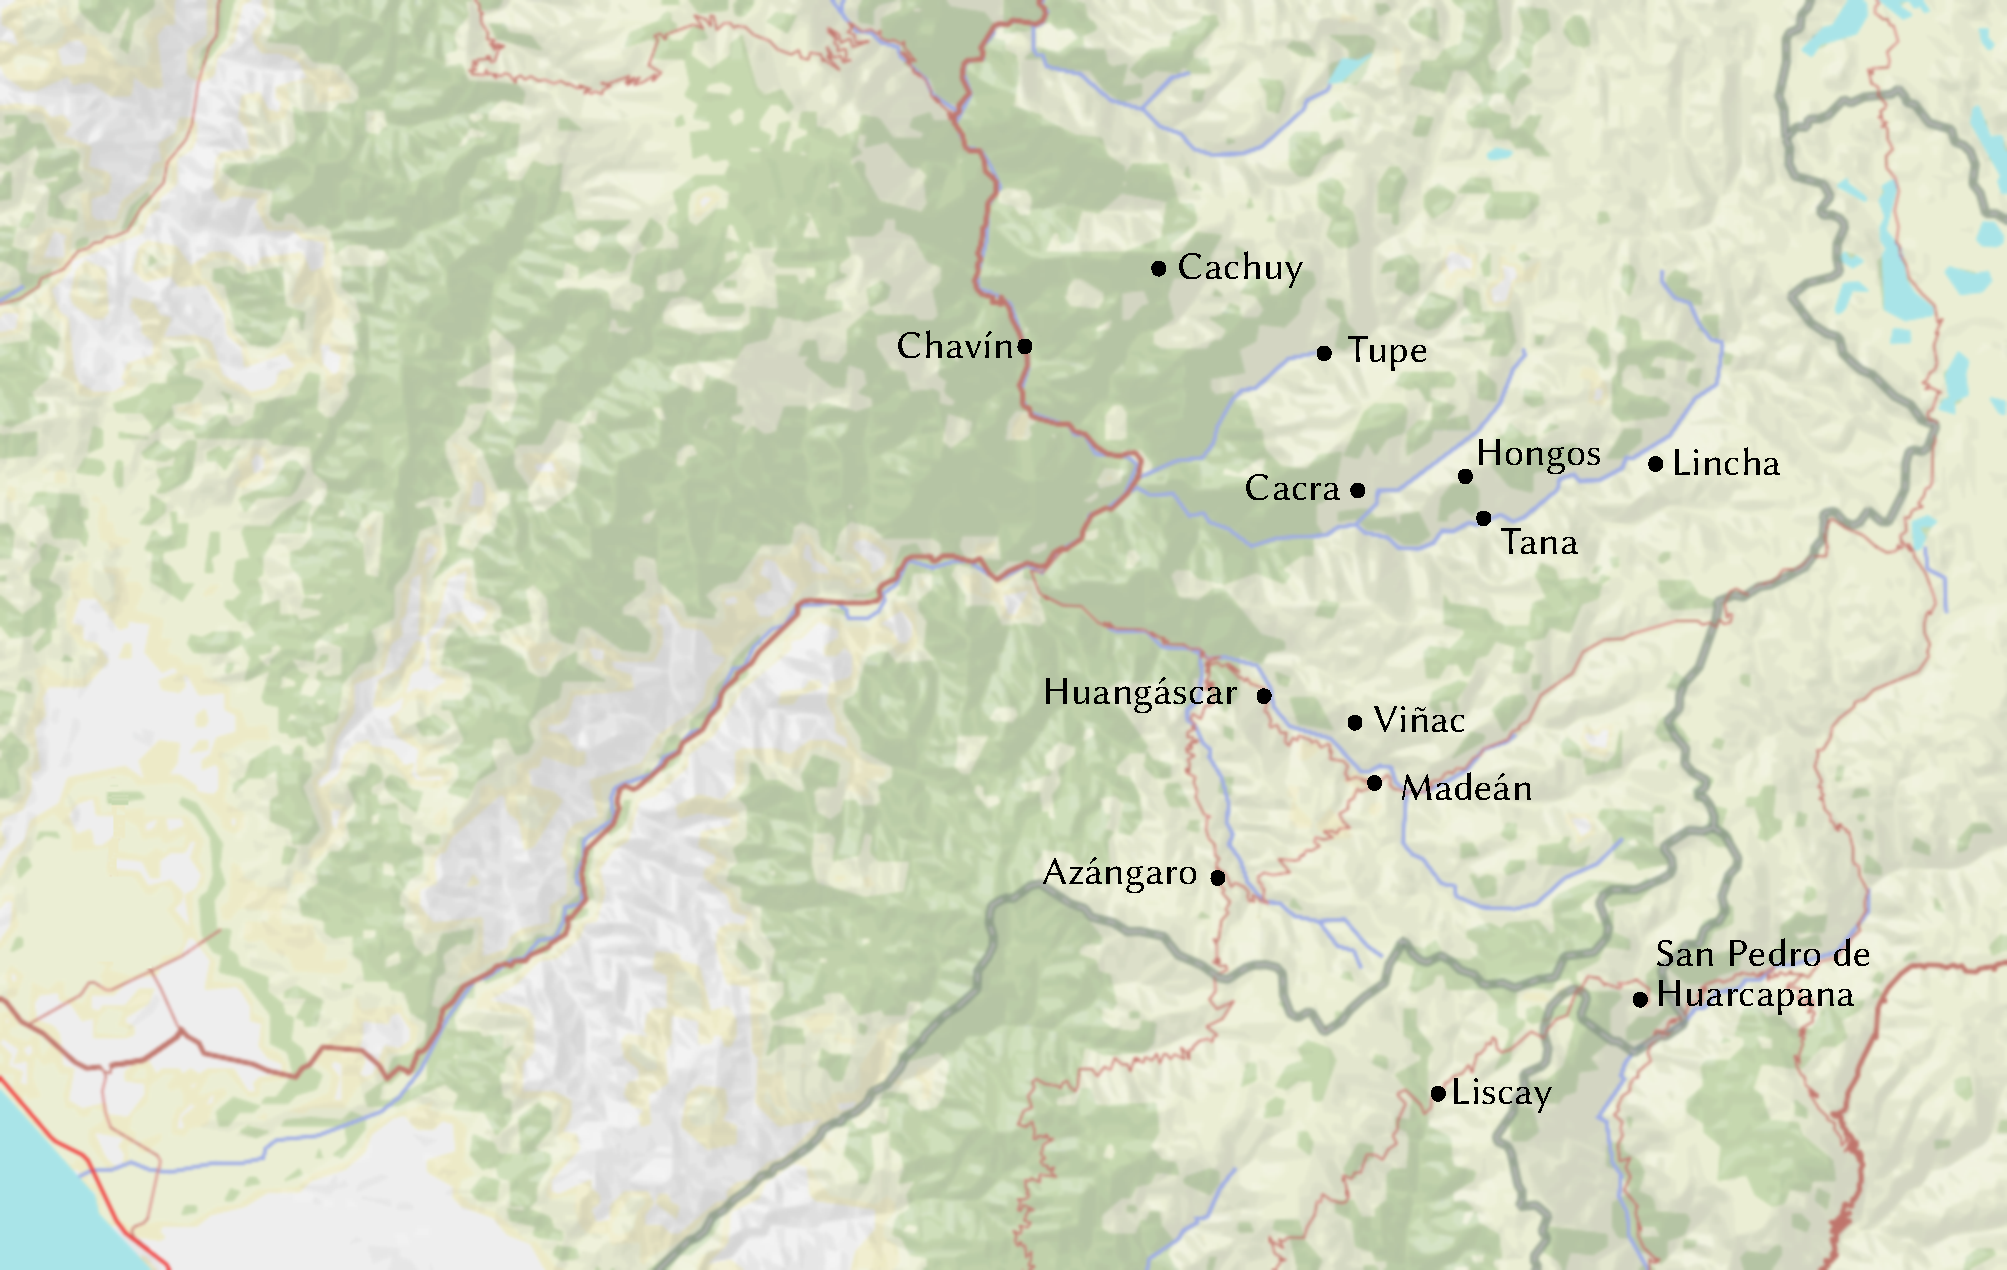
\includegraphics[width=\textwidth]{figures/madean3.pdf}
\end{figure}

No district except San Pedro is located more than one day’s walk from any other; in the case of San Pedro, it is two.\footnote{It is not irrelevant to the explanation of the dialect cleavages that this mountain range seems to block the movement of brides from one set of districts to another. Until very recently, newlywed women generally only moved from one town to another within the same valley.} The four districts that lie within the province of Yauyos center at 12°62′S and 75°7′W. The principal towns of all the districts except Chocos, Huangáscar, and Tana sit at altitudes around 3300 meters, while those of Chocos, Huangáscar, and Tana sit at just under 3000 meters. The relevant region can be contained within an area of 40~m\textsuperscript{2}; its highest peak reaches 5055~m.\footnote{There exists a series of topographical maps prepared and published in 1996 by the U.S. Defense Mapping Agency. Southern Yauyos is covered on the section labeled Tupe\index[sub]{Tupe} and identified Series 1745, Sheet J632, Edition -1 DMA.}

\section{Endangerment}\label{sec:endangerment}
At the date of this writing, the UNESCO\index[aut]{UNESCO} classifies Yauyos as critically \index[sub]{endangerment}endangered.
% ,         (\url{http://multitree.linguistlist.org/trees/10504@124926}).
The 18th edition of \textit{Ethnologue} \citep{ethnologue}\index[aut]{Ethnologue}\index[aut]{Lewis, M. Paul}, however, tags it as “moribund.” Although, as I see it, there is no real likelihood that any dialect of Yauyos will ever be revived, it is early yet to declare it moribund. I estimate that there are about twenty teens who understand the Viñac and San Pedro dialects, as well as many as 80 adults in their forties and fifties who can still speak it relatively fluently. Moreover, although its use is now generally restricted to the discussion of every-day and ritual activities, it is still used frequently among the oldest speakers.

The 1993 Peru census counted~1,600 speakers,~25\%{} of them over~65 \citep[121]{Chirinos01}. \index[aut]{Chirinos-Rivera, Andrés}That census, however, did not distinguish between speakers of Yauyos and speakers of other Quechuan languages who resided in the province~(Chirinos-Rivera, p.c.). This is crucial to the assessment of the data on the Quechua-speaking population of the north of the province. Although there are many Quechua-speaking migrants there --~principally from \ili{Huancayo}, the town with which the north has the most commercial contact~-- I was unable to locate any speakers of the dialects indigenous to the area. Further, population data in the province tend to be exaggerated for several reasons. First, people who emigrated from the region years or even decades ago remain, nevertheless, officially resident there for reasons of convenience. Second, death certificates are often not issued for the deceased. Less than ten years before that survey --~still, to my knowledge, the most recent~-- electricity had yet to come to the Andean towns of southern Yauyos and the only physical connections between those towns to the rest of the world were three~40-kilometer dirt paths that wound their perilous way~2,000 meters down the canyon. Since that time, the Peruvian government has installed electricity in the region and widened the perilous dirt paths into perilous dirt roads.\footnote{In the space of just one year, spanning~2012 and~2013, fourteen people died in six separate accidents in the region when their vehicles fell from the road down the canyon.} TelMex and Claro now offer cable television, and buses come and go on alternate days. In short, the isolation that had previously preserved the Quechua spoken in the region has been broken and the language now counts, according to my estimates, fewer than~450 speakers, most over~65, and all but the most elderly fully bilingual in Spanish. 

The drastic reduction in the number of speakers can also be attributed to the Shining Path\index[sub]{Shining Path}. During the~1980’s and early~1990’s, the period during which the Maoist army terrorized the region, there was a large-scale exodus, particularly of young people, who ran to escape forced conscription. Many never returned, remaining principally in the coastal cities of Cañete and Lima. Theirs was the last generation to learn Quechua to any degree. Currently, there are a few children --~those who live with their grandmothers or great-grandmothers in the most isolated hamlets~-- with a passive knowledge of the language. The youngest speakers, however, are in their late thirties.

Quechuan as a language family is not currently endangered, and other Quechuan languages are well-documented. Estimates of the numbers of Quechuan speakers range between~8.5 and~10 million, and, although Quechua is being pushed back by Spanish in many areas, the majority dialects of its major varieties --~\ili{Ancash}, \ili{Ayacucho}, \il{Bolivian Quechua}Bolivian, \ili{Cuzco}, Ecuadorian\footnote{It is worth noting that much of the diversity internal to these languages is being lost, as one anonymous reviewer points out.}~-- are quite viable \citep[168]{Adelaar04}.\index[aut]{Adelaar, Willem F. H.}\index[aut]{Muysken, Pieter C.} Paradoxically, however, the viability of the major varieties is coming at the expense of the viability of the minor varieties. \citet[14]{Adelaar08}\index[aut]{Adelaar, Willem F. H.} writes: “If Quechua will survive, its speakers will probably be users of four of five of the most successful dialects, most of which belong to Quechua IIB and IIC.” The dialects of southern Yauyos, classified as either \QI{} or \QIIA, and other minor Quechuan languages are rapidly disappearing.

\section{Existing documentation}\label{sec:documentation}
\citet{Echerd74}\index[aut]{Echerd, Stephen M.} and \citet{Brougere92}\index[aut]{Brougère, Anne-Marie} supply some socio-linguistic data on Yauyos. There is also a book of folktales, in Spanish, collected in the region in the~1930’s and~1940’s: \spanish{Apuntes para el folklor de Yauyos} \citep{Varilla}.\index[aut]{Varilla Gallardo, Brígido} Yauyos is mentioned in the context of two dialectological studies of Quechua by \citet{Torero68,Torero74}\index[aut]{Torero, Alfredo}.

With these exceptions, all that is known about Yauyos we owe to the French researcher Gerald Taylor.\index[aut]{Taylor, Gerald} Taylor’s PhD dissertation describes the morphology of Laraos, a northern dialect of Yauyos. This work was republished or excerpted, sometimes with revisions, in \citet{Taylor84,Taylor90,Taylor94a,Taylor94b}. \citet{Taylor87a} supplements the data on Laraos with data on Huancaya, and
\citet{Taylor90,Taylor00} provides a comparison of all seven dialects on the basis of eight grammatical elements and fifty lexical items. Finally, \citet{Taylor87b,Taylor87c,Taylor91} transcribes and translates several folktales into Spanish and French.


\section{The dialects of Yauyos}\label{sec:dialectsofyauyos}
Yauyos groups together various dialects that, although mutually intelligible, differ in ways that are relevant both to the classification of Yauyos as well as to the current paradigm for the classification of the Quechuan languages generally. That classification is highly contested, and, indeed, has been since the first proposals were suggested in the 1960s \citep[See in particular][]{Landerman91}.\index[aut]{Landerman, Peter}

% TREE
% http://lingweb.eva.mpg.de/quechua/Eng/Cpv/Locations.htm#TheTraditionalQuechuaFamilyTree
% Adapted from
\begin{figure}[!ht]
\centering
\il{Proto-Quechua}\il{Huaihuash}\il{Huailay}\il{Huailas}\il{Conchucos}\il{Ap-am-ah}\il{Alto Pativilca}\il{Alto Marañón}\il{Alto Huallaga}\il{Yaru}\il{Jauja}\il{Huanca}\il{Huangáscar}\il{Topará}\il{Pacaraos}\il{Huampuy}\il{Yungay}\il{Laraos}\il{Lincha}\il{Apurí}\il{Chocos}\il{Madeán}\il{Cañaris}\il{Incahuasi}\il{Cajamarca}\il{Chinchay}\il{Amazonas}\il{San Martín Quechua}\il{Loreto}\il{Ecuadorian Quechua}\il{Colombian Quechua}\il{Ayacucho}\il{Cuzco}\il{Puno}\il{Bolivian Quechua}\il{Argentinan Quechua}
\resizebox{\textwidth}{!}{%
\begin{tikzpicture}[%
treenode/.style = {align=center, inner sep=2ex, text centered},
level 1/.style={sibling distance = 52ex, level distance =12ex,font=\Large}, 
level 2/.style={sibling distance = 28ex, level distance =10ex,font=\large},
level 3/.style={sibling distance = 13ex, level distance =8ex,font=\normalsize\sc},
level 4/.style={treenode,text width=12ex, level distance =6ex,font=\small,below},
level 5/.style={level distance =4ex,edge from parent/.style={draw=none,below}}]
\node[font=\Large] {PROTO-QUECHUA}
  child{node {HUAIHUASH (QI)} 
    child{node {CENTRAL} 
      child{node {Huailay} 
        child{node {Huailas}
          child{node {Conchucos}
          }
        }
      }
      child{node {Ap-am-ah}
        child{node {Alto Pativilca}
          child{node {Alto Marañón} 
            child{node {Alto Huallaga}
            }
          }
        }
      }
      child{node {Huancay} 
        child{node {Yaru}
          child{node {Jauja \&{} Huanca} 
            child{node {Huangáscar \&{} Topará} 
            }
          }
        }
      }
    }
    child{node {PACARAOS}
      child{
        child{node {Pacaraos}
        }
      }
    }
  }
  child{node {HUAMPUY (QII)}
    child{node {QIIA (‘YUNGAY’)} 
      child{node {Central}
        child{node {Laraos}
          child{node {Lincha}
            child{node {Apurí}
              child{node {Chocos}
                child{node {Madeán}
                }
              }
            }
          }
        }
      }
      child{node {Northern}
        child{node {\ili{Cañaris} \&{} Incahuasi}
          child{node {Cajamarca}
          }
        }
      }
    }
    child{node {QIIB-C (‘CHINCHAY’)}
      child{node {Northern}
        child{node {Amazonas}
          child{node {San Martín}
            child{node {Loreto}
              child{node {Ecuador: Highland \&{} Lowland}
                child{node {Colombia}
                }
              }
            }
          }
        }
      }
      child{node {Southern}
        child{node {Ayacucho}
          child{node {\ili{Cuzco}, Puno \&{} Bolivia}
            child{node {Argentina}
            }
          }
        }
      }
    }
  };
\end{tikzpicture}}
\caption{Quechuan languages family tree}\label{Fig1}
% \raggedright
% {\scriptsize Adapted from source:\url{http://lingweb.eva.mpg.de/quechua/Eng/Cpv/Locations.htm#TheTraditionalQuechuaFamilyTree} }
\end{figure}

The Province is located on the border between the two large, contiguous zones where languages belonging to the two great branches of the Quechua language family are spoken: the “Quechua I” (Torero)\index[aut]{Torero, Alfredo} or “Quechua B” (Parker)\index[aut]{Parker, Gary J.} languages are spoken to its north; the “Quechua~II” or “Quechua~A” languages, to its south, as the map in Figure~\ref{Figcomp} shows.

\begin{figure}

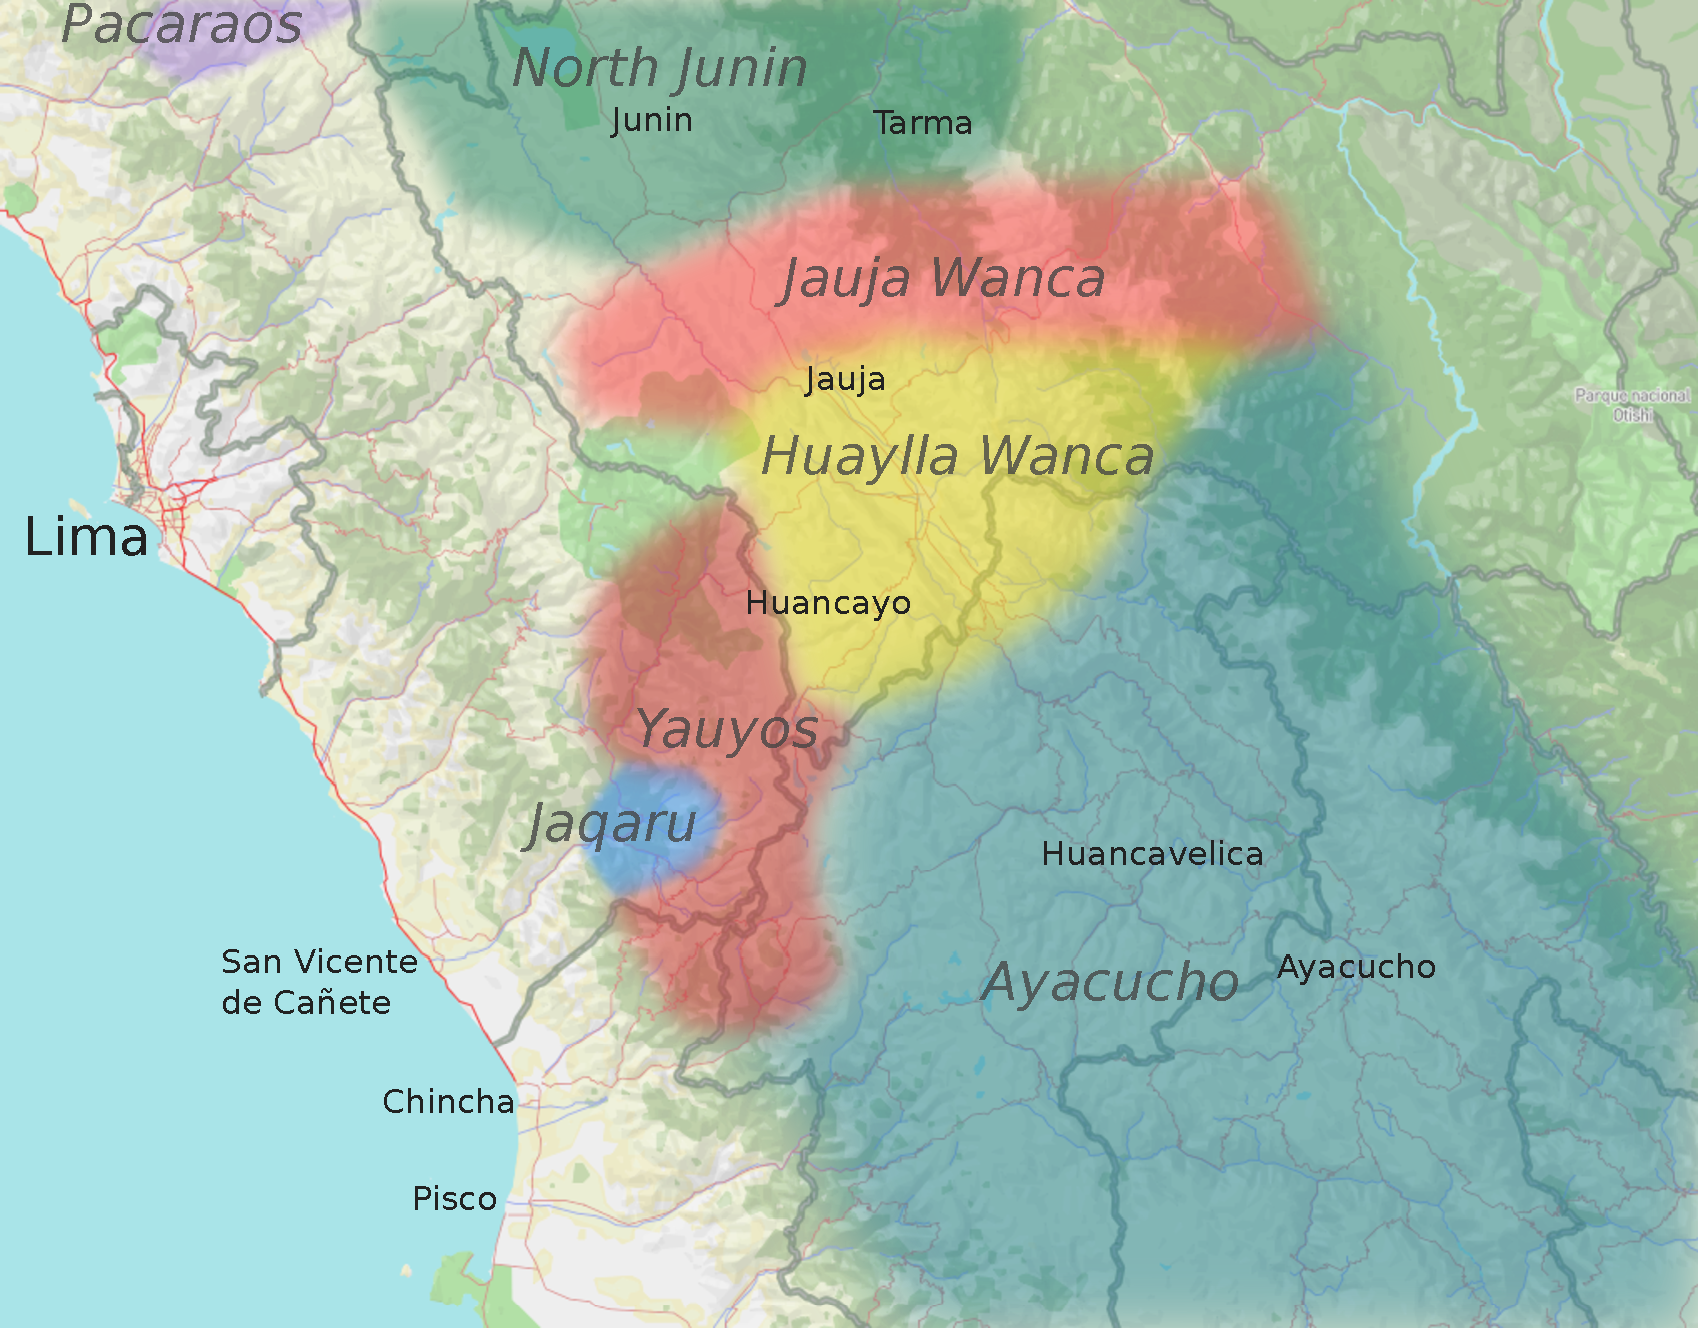
\includegraphics[width=0.889\textwidth]{figures/largerregion2.pdf}

\caption{Peruvian languages map}\label{Figcomp} 

\end{figure}

For reasons detailed in \sectref{sec:classification}, the model that divides the Quechuan family tree into two principal branches doesn’t apply very well to Yauyos, as its different dialects manifest different characteristics of both of branches. Yauyos is, of course, not alone in this, not in the least because the division of the languages into two branches was, arguably, based on rather arbitrary criteria in the first place \citep[See in particular][]{Landerman91}.\index[aut]{Landerman, Peter} The significance of Yauyos lies in the fact that it may represent the “missing link” between the two \citep[See in particular][]{Heggarty07}\index[aut]{Heggarty, Paul}. There exist three proposals in the literature --~\citet{Taylor00,Torero74,ethnologue}\index[aut]{Taylor, Gerald}\index[aut]{Torero, Alfredo}\index[aut]{Lewis, M. Paul}~-- with regard to the grouping of the province’s fifteen districts into dialect bundles. \citet[105]{Taylor00}\index[aut]{Taylor, Gerald} counts seven varieties of Yauyos Quechua, dividing these into two groups along a north-south axis. In the north are the dialects of Alis/Tomas, Huancaya/Vitis, and Laraos; in the south, those of Apurí/Chocos/Madeán/Viñac, Azángaro/Huangáscar, Cacra/Hongos, and Lincha/Tana. Taylor classes four of these dialects --~the northern dialects of Alis/Tomas\il{Alis}\il{Tomas} and Huancaya/Vitis\il{Huanca}\il{Vitis} and the southern dialects of Azángaro/Huangáscar\il{Azángaro}\il{Huangáscar} and Cacra/Hongos\il{Cacra}\il{Hongos}~-- as belonging to the \QI{} branch; he classes the remaining three --~Laraos\il{Laraos} in the north as well as Apurí/Cho\-cos/Madeán/Víñac\il{Apurí}\il{Chocos}\il{Madeán}\il{Víñac} and Lincha/Tana\il{Lincha}\il{Tana} in the south~-- as belonging to \QII. \citet{Torero74}\index[aut]{Torero, Alfredo} counted only six dialects, excluding Azángaro/Huangáscar\il{Azángaro}\il{Huangáscar} from the catalogue, classing it independently among the \QI{} dialects along with with Chincha’s Topará\il{Topará}. Ethnologue, like Taylor, includes Azángaro/Huangascar and adds, even, an eighth dialect, that of San Pedro de Huacarpana, spoken on the Chincha side of the Yauyos-Chincha border. Ethnologue further differs from Taylor in putting Apurí in a group by itself; and it differs from both Taylor and Torero in grouping Chocos with Azángaro/Huangáscar. My research supports Taylor’s grouping of Apurí with Madeán and Viñac; it also supports Ethnologue’s inclusion of San Pedro de Huacarpana among the dialects of Yauyos. San Pedro is located immediately to the north-east of Madeán and Azángaro, at less than a days’ walk’s distance. Although formerly counted a part of the Department of Lima and the Province of Yauyos, a redrawing of political boundaries placed San Pedro on the Ica side of the contemporary Ica-Lima border. During the colonial period, the Province of Yauyos was larger and included parts of what are now the Provinces of Chincha and Castrovirreyna (Huancavelica) \citet[1.1.3.2.7]{Landerman91}\index[aut]{Landerman, Peter N.}. Apurí, like its neighbors Viñac and Madeán, uses \phono{-ni} and \phono{-y} to indicate the first-person singular in the verbal and substantive paradigms; they also use \phono{-rqa} and \phono{-sa} to indicate the past tense and perfect. The first pair of characteristics set the Madeán/Viñac and Lincha/Tana dialects apart from the other three; the second pair of characteristics sets Madeán/Viñac apart from Lincha/Tana. Chocos, like its neighbors Huangáscar and Azángaro, uses vowel length to indicate the first-person singular in the verbal and substantive paradigms.

\section{Classification}\label{sec:classification}\index[sub]{classification}
\largerpage %longdistance
Yauyos Quechua was dubbed by Alfredo Torero (\citeyear{Torero74})\index[aut]{Torero, Alfredo} a “supralect” and its most careful student, Gerald Taylor,\index[aut]{Taylor, Gerald} referred to it as a “mixed” language (\citealt[2]{Taylor90}, \citealt[105]{Taylor00}). Indeed, the designation of Yauyos as a language may seem, at first, to be no more than a relic of the first classifications of the Quechuan languages not by strictly linguistic criteria but, rather, by geographic criteria. Yauyos is located on the border between the two large, contiguous zones where the languages of the two different branches of the Quechuan language family are spoken. \QI{} is spoken immediately to the north, in the Department of \ili{Junín} and the north of the Department of Lima; \QII, immediately to the south, in the Departments of Huancavelica and \ili{Ayacucho}. Yauyos manifests characteristics of both branches. Take first-person marking. Three dialects, Azángaro-Chocos\footnote{I am very grateful to Peter Landerman for correcting me with regard to the classification of Chocos, which I had originally misclassified with Madeán and Viñac.}-Huangáscar~(\ACH), Cacra-Hongos (\CH), and San Pedro~(\SP), use the same marking~(vowel length) for the first person in both nominal and verbal paradigms\footnote{Crucially, though, vowel length is not distinctive anywhere else in the grammar or lexicon of these dialects. For example, these dialects use the \QII{}~\phono{-naya},~\phono{-raya}, and~\phono{-paya}, not the \QI{}~\phono{-na:},~\phono{-ra:}, and~\phono{-pa:} to mark the desiderative, passive, and continuative, respectively. And all districts but Cacra use~\phono{tiya-}, not~\phono{ta:-} ‘sit’, again sorting with the \QII{} languages.} and mark the first-person object with~\phono{-ma}. These are the two characteristics that define a Quechuan language as belonging to the \QI{}~(also called Quechua B or~\textit{Huaihuash}) branch. The other two dialects, Apurí-Madeán-Viñac~(\AMV) and Lincha-Tana~(\LT), mark the first person differently in the nominal and verbal paradigms~(with~\phono{-y} and~\phono{-ni}, respectively) and mark first-person object with~\phono{-wa}. These two dialects, then, sort with the \QII{}~(A/\textit{Huampuy})\il{Huampuy} languages. Indeed, the first three are classed as \QI{}~(specifically, Central\textit{-Huancay}) and the other two, \QII{}~(specifically~\textit{Yunagay}-Central) \citep[247]{CerroP87}.\index[aut]{Cerrón-Palomino, Rodolfo M.} Nevertheless, the “\QI” dialects, \ACH, \CH, and \SP, manifest few of the other traits that set the \QI{} languages apart from the \QII{} languages. They do use~\phono{ñuqakuna}\index[sub]{nuqakuna@\phono{ñuqakuna}} in place of \phononb{ñuqayku}\index[sub]{nuqayku@\phono{ñuqayku}} to form the first person plural exclusive as well as~\phono{-pa(:)ku} to indicate the plural. Crucially, however, so do both the “\QII” \SYQ{} dialects.\footnote{The \CH{} dialect is unique in using~\phono{-traw} in alternation with both~\phono{-pi} and~\phono{-pa} for the locative.} And none of the five manifest any other of the principal traits that generally set the \QI{} languages apart from the rest. None use~\phono{-naw} in place of~\phono{-Sina} to form the comparative,~\phono{-piqta} in place of~\phono{-manta} to form the ablative, or~\phono{-naq} in place of~\phono{-shqa} to form the narrative past; and none except for Cacra uses~\phono{-r} (realized \textipa{[l]}) in place of~\phono{-shpa} to form same-subject subordinate clauses. Now, the two “\QII” \SYQ{} dialects manifest several of the traits that set the \QIIC{}~(\textit{Chínchay Meridional}) languages apart from the rest. Like the \QIIC{} languages, the \AMV{} and \LT{} dialects use the diminutive~\phono{-cha}, the emphatic~\phono{-ari}, the assertive~\phono{-puni}, and the alternative conditional~\phono{-chuwan}; the \AMV{} dialect additionally uses the alternative conditional~\phono{-waq.} Crucially, however, the three “\QI” \SYQ{} dialects, too, use three of these:~\phono{-cha},~\phono{-ari} and~\phono{-chuwan}. Further, all five share with \ili{Ayacucho} Q the unique use of the evidential modifier~\phono{-ki}. None of the five manifest any of the other defining traits of the \QIIC{} languages: none uses~\phono{-ku} to indicate the first-person plural exclusive or the third-person plural; nor does any use~\phono{-chka}\footnote{Although all use~\phono{-chka}, unproductively except in \SP, to indicate simultaneous action that persists in time.} to form the progressive or~\phono{-nka} to form the distributive. Further, none suffered the fusion of \textipa{*/tr/} with \textipa{*/ch/} or \textipa{*/sh/} with \textipa{*/s/}. (See \citet[226--248]{CerroP87} on the defining characteristics of the various Quechuan languages)\index[aut]{Cerrón-Palomino, Rodolfo M.} Rather, the dialects of Southern Yauyos are mutually intelligible, and they together share characteristics that set them apart from all the other Quechuan languages. With the single exception that \CH{} uses the accusative form~\phono{-Kta} in place of~\phono{-ta}, all five dialects employ the same case system, which includes the unique ablative form~\phono{-paq} and unique locative \phono{-pi}. All dialects use the progressive form~\phono{-ya};\footnote{One of many attested reductions from *-\phono{yka}: (\phono{-yka:}, \phono{-yka}, \phono{-yga}, \phono{-ycha:}, \phono{-yya:}, \phono{-yya-}, \phono{-ya:}, and \phono{-ya}) \citep[213--219, 260--268, 290]{Hintz}. I am grateful to an anonymous reviewer for pointing this out to me.} all employ the plural~\phono{-kuna} with non-exhaustive meaning; and all employ the same unique system of evidential modification~(see \sectref{ssec:evidmodifi}). 
\largerpage
Further, with a single exception,\footnote{In the \CH{} dialect, as in neighboring \ili{Junín}, the protomorphemes \textipa{*/r/}, \textipa{*/s/}, and \textipa{*/h/} are sometimes realized as \textipa{[l]}, \textipa{[h]}, and \textipa{[sh]}, respectively. I have no explanation for why these alternations occur in some cases but not in others. Indeed, it may be the case that where \CH{} differs from the rest of the dialects in that it employs \textipa{*/sh/}where they employ \textipa{*/h/, it is the former that preserves the original form.}} the five dialects are uniform phonologically, all employing a highly conservative system\footnote{An anonymous reviewer points out that other Quechuan languages, \ili{Corongo} among them, for example, are more conservative than Yauyos with respect to some features, including the preservation of the protoform *ñ in *ñi- ‘say’ and ña:-ña ‘right now’. \ili{Sihuas}, too, preserves elements of proto Quechua not found in Yauyos. In contrast, while Yauyos preserves a few proto-Quechua features not found in either \ili{Corongo} or \ili{Sihuas}, it also manifests others that reflect innovations likely adopted from neighboring QII languages.} that retains all those phonemes hypothesized by Parker and Cerrón-Palomino to have been included in the Proto-Quechua (see \sectref{sec:phoinvmor}). Table~\ref{Tab1}, below, summarizes this information. Please note that the table presents a somewhat idealized portrait and that the characteristics it posits as belonging exclusively to \QII{} may sometimes be found in \QI{} languages as well. Exceptions of which I am aware are signaled in notes to the table.

% TABLE 1
\begin{table}
\renewcommand*{\arraystretch}{0.9}
\centering
\caption{Use of \QI, \QII{} and local structures in the five \SYQ{} dialects}\label{Tab1}
\footnotesize
\begin{tabularx}{0.9\textwidth}{Xccccc}
\lsptoprule
 &\CH &\ACH &\SP &\AMV &\LT\\
\midrule
%
1Singular nominal inflection%
&\Qgreen{\it -:} &\Qgreen{\it -:} &\Qgreen{\it -:} &\Qblue{\it -y} &\Qblue{\it -y} \\
%
1Singular verbal inflection%
&\Qgreen{\it -:} &\Qgreen{\it -:} &\Qgreen{\it -:} &\Qblue{\it -ni} &\Qblue{\it -ni} \\
%
1Singular object inflection%
&\Qgreen{\it -ma} &\Qgreen{\it -ma} &\Qgreen{\it -ma} &\Qblue{\it -wa} &\Qblue{\it -wa} \\
%
1Plural exclusive pronoun~\phono{ñuqakuna}%
&\Qgreen{yes} &\Qgreen{yes} &\Qgreen{yes} &\Qgreen{yes} &\Qgreen{yes} \\
%
Fusion of \textipa{*/ch/} and \textipa{*/tr/}\tabfoot{a}%
&\Qgreen{no} &\Qgreen{no} &\Qgreen{no} &\Qgreen{no} &\Qgreen{no} \\
%
Fusion of \textipa{*/s/} and \textipa{*/sh/}%
&\Qgreen{no} &\Qgreen{no} &\Qgreen{no} &\Qgreen{no} &\Qgreen{no} \\
%
\lsc{s}>\lsc{o} inflection order \lsc{num-o-tns-s}%
& \Qgreen{yes} &\Qgreen{yes} &\Qgreen{yes} &\Qgreen{yes} &\Qgreen{yes} \\
%
Vowel length distinctive elsewhere\tabfoot{b}%
&\Qblue{no} &\Qblue{no} &\Qblue{no} &\Qblue{no} &\Qblue{no} \\
%
Same-subject subordinator~\phono{-shpa}\tabfoot{c}%
&\Qblue{yes} &\Qblue{yes\tabfoot{d}} &\Qblue{yes}&\Qblue{yes} &\Qblue{yes} \\
%
Narrative past inflection~\phono{-sHQa}%
&\Qblue{yes} &\Qblue{yes} &\Qblue{yes} &\Qblue{yes} &\Qblue{yes} \\
%
Comparative~\phono{-hina}%
&\Qblue{yes} &\Qblue{yes} &\Qblue{yes} &\Qblue{yes} &\Qblue{yes} \\
%
Diminutive~\phono{-cha}\tabfoot{e}%
&\Qblue{yes} &\Qblue{yes} &\Qblue{yes} &\Qblue{yes} &\Qblue{yes} \\
%
Emphatic~\phono{-ari}%
&\Qblue{yes} &\Qblue{yes} &\Qblue{yes} &\Qblue{yes} &\Qblue{yes} \\
%
1Plural Altern. Conditional~\phono{-chuwan}%
&\Qblue{yes} &\Qblue{yes} &\Qblue{yes} &\Qblue{yes} &\Qblue{yes} \\
%
2Singular Altern. Conditional~\phono{-waq}%
&\Qgreen{no} &\Qgreen{no} &\Qgreen{no} &\Qblue{yes} &\Qgreen{no} \\
%
Assertive~\phono{-puni}%
&\Qgreen{no} &\Qgreen{no} &\Qgreen{no} &\Qblue{yes} &\Qgreen{no} \\
%
Evidential modifier~\phono{-ki}\tabfoot{f}%
&\Qred{yes} &\Qred{yes} &\Qred{yes} &\Qred{yes} &\Qred{yes} \\
%
Locative~\phono{-pa}%
&\Qred{yes\tabfoot{g}}&\Qred{yes} &\Qred{yes} &\Qred{yes} &\Qred{yes} \\
%
Ablative~\phono{-paq}\tabfoot{h}%
&\Qred{yes} &\Qred{yes} &\Qred{yes} &\Qred{yes} &\Qred{yes} \\
%
Non-exhaustive~\phono{-kuna}%
&\Qred{yes} &\Qred{yes} &\Qred{yes} &\Qred{yes} &\Qred{yes} \\
%
Lateralization of \textipa{*/r/}%
&yes\tabfoot{j} &no &no &no &no\\
\lspbottomrule
\end{tabularx}
\begin{tabularx}{\textwidth}{@{~}r@{~}X@{~}}
\\[-2ex]
Note: &\\
\tabfoottext{a}{An anonymous reviewer points out that this is not exclusively a feature of \QII{} languages in that the fusion of */ch/ and */tr/ is attested in \ili{Huallaga}, a \QI{} variety.}
\tabfoottext{b}{With the exception of~\phono{-pa(:)ku}, where the long vowel distinguishes \lsc{jtacc} from \lsc{ben-refl}.}
\tabfoottext{c}{An anonymous reviewer points out that, although this may originally have been posited to be a defining characteristic of \QII{} languages, it is, in fact, far from such: \phono{-shpa} is common in several QI dialects: in \ili{Ancash}, it attested in \ili{Huaylas}; it is attested, also in Pachitea in \ili{Huanuco}.}
\tabfoottext{d}{Cacra but not Hongos also uses~\phono{-r} (realized \textipa{[l]}).}
\tabfoottext{e}{An anonymous reviewer points out that while diminutive \phono{-cha} is less productive in \QI{} than in \QII, it is still is common throughout \QI, \eg{} Victoria-Vitucha, Cabrito-Kapcha.}
\tabfoottext{f}{Also used in \ili{Ayacucho} (\QII).}
\tabfoottext{g}{Also uses~\phono{-traw} (\QI).}
\tabfoottext{h}{An anonymous reviewer points out that ablative \phono{-paq} is almost certainly derived from */-piq/ / */-pik/ via vowel harmony. The former is attested in \ili{Huaylas} and the latter in \ili{Corongo}. The other \phono{-pi}-initial forms in \QI{} (\phono{-pita}, -\phono{pi:ta}, -\phono{pikta}, -\phono{piqta}, among others) would have developed later via suffix amalgamation, similar to the formation of bipartite \phono{-manta} in \QII{} \citep[see, \eg,][]{hintz2000caracteristicas}.}
\tabfoottext{j}{Also occurs in \ili{Junín} (\QI).}\\[-1ex]
Key: &*:~\QI{} trait; †:~\QII/\QIIC{} trait; ‡:~trait shared by all \SYQ{} dilects not characteristic of either \QI{} or \QII/\QIIC.\\
\end{tabularx}
\end{table}

The case of Azángaro-Chocos-Huangáscar requires particular attention in this context. Torero (\citeyear{Torero68}:~293, \citeyear{Torero74}:~28--29)\index[aut]{Torero, Alfredo} classified Azángaro and Huangáscar as forming an independent group with Topará\il{Topará} (Chavín)\index[sub]{Chavín}, placing it among the \QI{} \phono{Huancay} languages. \citet[236]{CerroP87},\index[aut]{Cerrón-Palomino, Rodolfo M.} following Torero, cites five criteria for grouping Huangáscar with Topará. Both dialects, he writes, use \phono{-pa:ku} and~\phono{-:ri} to indicate the plural; both use~\phono{-shpa} in place of~\phono{-r} to form same-subject subordinate clauses; and both use~\phono{-tamu} to indicate completed action; the two dialects, further, are alike in using unusual locative and ablative case-marking. Only three of these claims are accurate. First, Huangáscar, as \citet{Taylor84}\index[aut]{Taylor, Gerald} already indicated, does not use~\phono{-:ri}. Second, Huangáscar and Topará may indeed both use unusual locative and ablative case marking, but, crucially, they do not use the same unusual case marking: Huangáscar uses~\phono{-pa} to indicate the locative while Topará uses~\phono{-man}; Huangáscar uses~\phono{-paq} to indicate the ablative while Topará uses~\phono{-pa}~(C.-P. himself points out these last two facts). Huangáscar does indeed use~\phono{-shpa} to form subordinate clauses and~\phono{-tamu} to indicate irreversible change. Crucially, however, so do all the dialects of southern Yauyos. In sum, there is no basis for grouping Huangáscar with Topará and not with the other dialects of \SYQ. Torero’s data were never corroborated; indeed, the findings of Taylor and Landerman, the scholars who have most thoroughly studied Yauyos before now,\footnote{An anonymous reviewer points out that Martha Hardman, Steve Echerd, Rick Floyd, Conrad Phelps --~in addition to several students from Universidad San Marcos~-- have given Yauyos extensive attention, although they may not have added to the storehouse of data on the language.} contradict those of Torero.

\SYQ{} is not a jumble of dialects that, were it not for geographical accident, would not be classed together; it is, rather, a unique, largely uniform language. Although I myself do not believe that the current paradigm can be maintained, I have tried to present the data in a way that remains as neutral as possible with regard to the question of how the internal diversity within the Quechuan language family is best characterized, and, in particular, with regard to the question of whether or not the various Quechuan languages are helpfully construed as belonging to one or the other of two branches of a family tree \citep[See in particular][]{Adelaar08}.\index[aut]{Adelaar, Willem F. H.} I leave it to other scholars to interpret the data as they see fit. That said, as long as it is maintained, the current paradigm should be revised to more accurately reflect the relationships of \SYQ{} with/to the languages currently named on the Quechuan family tree as it is currently drawn. That tree groups nine of the eleven districts of southern Yauyos into five sets, assigning each of these sets the status of an independent language. Moreover, two of these sets are actually singletons, as Chocos is listed independent of \mbox{(Azángaro-)}Huangáscar, to which it is identical, and Apurí is listed independent of Madeán(-Viñac), to which it is identical. (Cacra-Hongos, the set that would deserve independent placement, if any did, appears nowhere at all). The fact that all these “languages” are completely mutually intelligible does not justify this. It further seems unjustified to place the Quechua of single villages on the level of that of whole nations --~Bolivia and Ecuador. I suggest, therefore, that Chocos be joined with \mbox{(Azángaro-)}Huangáscar, and Apurí with Madeán(-Viñac). The first of these new triplets, Azángaro-Chocos-Hunagáscar, should be mutated to join the other “languages” of southern Yauyos, under the category \textit{Central Yungay}. The four sets should, further, be collapsed and the resulting set called \textit{Southern Yauyos}. The revised (pruned) tree would then be as in Figure~\ref{Fig1rev}. In the event that it be necessary to honor the internal diversity that would be obscured by this move, note may simply be made to the fact that this “new” language counts multiple dialects. In this case, Cacra-Hongos and San Pedro de Huacarpana would have to be listed among these.\footnote{I regret having to list Laraos independently here, as I believe it is possible to make a convincing argument for its inclusion as a dialect of Southern Yauyos. Nothing in this volume, however, directly speaks to that question. I plan to address it explicitly in a future paper.}

% REVISED TREE
% http://lingweb.eva.mpg.de/quechua/Eng/Cpv/Locations.htm#TheTraditionalQuechuaFamilyTree
% Adapted from
\begin{figure}[!ht]

\il{Proto-Quechua}\il{Huaihuash}\il{Huailay}\il{Huailas}\il{Conchucos}\il{Ap-am-ah}\il{Alto Pativilca}\il{Alto Marañón}\il{Alto Huallaga}\il{Yaru}\il{Jauja}\il{Huanca}\il{Pacaraos}\il{Huampuy}\il{Yungay}\il{Laraos}\il{Cañaris}\il{Incahuasi}\il{Cajamarca}\il{Chinchay}\il{Amazonas}\il{San Martín Quechua}\il{Loreto}\il{Ecuadorian Quechua}\il{Colombian Quechua}\il{Ayacucho}\il{Cuzco}\il{Puno}\il{Bolivian Quechua}\il{Argentinan Quechua}
\resizebox{\textwidth}{!}{%
\begin{tikzpicture}[%
treenode/.style = {align=center,inner sep=2ex,text centered},
level 1/.style={sibling distance=52ex,level distance=12ex,font=\Large}, 
level 2/.style={sibling distance=28ex,level distance=10ex,font=\large},
level 3/.style={sibling distance=13ex,level distance=8ex,font=\normalsize\sc},
level 4/.style={treenode,text width=12ex,level distance=6ex,font=\small,below},
level 5/.style={level distance=4ex,edge from parent/.style={draw=none,below}}]
\node[font=\Large] {PROTO-QUECHUA}
  child{node {HUAIHUASH (QI)} 
    child{node {CENTRAL} 
      child{node {Huailay} 
        child{node {Huailas}
          child{node {Conchucos}
          }
        }
      }
      child{node {Ap-am-ah}
        child{node {Alto Pativilca}
          child{node {Alto Marañón} 
            child{node {Alto Huallaga}
            }
          }
        }
      }
      child{node {Huancay} 
        child{node {Yaru}
          child{node {Jauja \&{} Huanca} 
          }
        }
      }
    }
    child{node {PACARAOS}
      child{
        child{node {Pacaraos}
        }
 	  }
    }
  }
  child{node {HUAMPUY (QII)}
    child{node {QIIA (‘YUNGAY’)} 
      child{node {Central}
        child{node {Laraos}
          child{node {Southern Yauyos}
          }
        }
      }
      child{node {Northern}
        child{node {\ili{Cañaris} \&{} Incahuasi}
          child{node {Cajamarca}
          }
        }
      }
    }
    child{node {QIIB-C (‘CHINCHAY’)}
      child{node {Northern}
        child{node {Amazonas}
          child{node {San Martín}
            child{node {Loreto}
              child{node {Ecuador: Highland \&{} Lowland}
                child{node {Colombia}
                }
              }
            }
          }
        }
      }
      child{node {Southern}
        child{node {Ayacucho}
          child{node {\ili{Cuzco}, Puno \&{} Bolivia}
            child{node {Argentina}
            }
          }
        }
      }
    }
  };
\end{tikzpicture}}

\caption{Quechuan languages family tree revised}\label{Fig1rev}
\raggedright
{\scriptsize Adapted from source: \url{http://lingweb.eva.mpg.de/quechua/Eng/Cpv/Locations.htm#TheTraditionalQuechuaFamilyTree}}
\end{figure}

\section{Presentation}\label{sec:presentation}
To facilitate comparison with other Quechuan languages, the presentation here follows the structure of the six Quechua grammars published by the Peruvian government in~1976. Readers familiar with those grammars will note the obvious debt this one owes to those: it follows not just their format, but also, in large part, their analysis. The six~1976 grammars cover the Quechuas of \ili{Ancash}, \ili{Ayacucho}, \ili{Cajamarca}, \ili{Cuzco}, \ili{Huanca} and \il{San Martín Quechua}San Martín. \citep{Parker76gram,Soto76a,Quesada76,Cusihuaman76,CerroP76a,Coombs76}.\index[aut]{Parker, Gary J.}\index[aut]{Soto Ruiz, Clodoaldo}\index[aut]{Quesada Castillo, Félix}\index[aut]{Cusihuamán Gutiérrez, Antonio}\index[aut]{Cerrón-Palomino, Rodolfo M.}\index[aut]{Coombs, David}\index[aut]{Coombs, Heidi}\index[aut]{Weber, Robert} Other published grammars of Quechuan languages include \citet{Herrero78}\index[aut]{Herrero, Joaquín}\index[aut]{Sánchez de Lozada, Federico} on \ili{Bolivian Quechua}; \citet{Catta94}\index[aut]{Catta, Javier} on \ili{Ecuadorian Quechua}; \citet{Taylor94a}\index[aut]{Taylor, Gerald} on \ili{Ferreñafe}; \citet{Weber89}\index[aut]{Weber, David} on \ili{Huallaga}~(\ili{Huanuco});\footnote{Thanks to an anonymous reviewer for pointing this out. \citet{Hintz} supplies a grammar of aspect and related categories in Quechua, especially South \ili{Conchucos} Quechua (\ili{Ancash}).} \citet{Cole82}\index[aut]{Cole, Peter} on \ili{Imbabura}; \citet{Adelaar77}\index[aut]{Adelaar, Willem F. H.} description of \ili{Tarma} Quechua and his (\citeyear{Adelaar86}) morphology of \ili{Pacaraos}; 
as well as the surveys and compilations of \citet{CerroP87,CerroP90}\index[aut]{Cerrón-Palomino, Rodolfo M.}\index[aut]{Solís-Fonesca, Gustavo}, and \citet{Cole94}\index[aut]{Cole, Peter}\index[aut]{Hermon, Gabriella}\index[aut]{Martín, Mario D.}.

Words and phrases appearing in italics --~\phono{like this}~-- are in Quechua. English and Spanish interpretations appear in single quotation marks --~‘like this’. Interpretations are sometimes given in Spanish --~the language I used with my consultants\footnote{Indeed, all English glosses are my translations from the Spanish glosses my consultants originally supplied. In most cases, the Spanish translations reflected the syntax and semantics of the original Quechua. I sacrificed this in preparing the the English glosses that appear here. I made this choice because the more literal glosses are standard in Andean Spanish --~in structures like the possessive ‘su n de a’ (‘his \lsc{n} of a’)~-- they would not be standard in any English dialect of which I am aware.} --~as well as English. Transformations (illustrations of changes indicated as a result of morphological processes referenced) are indicated with arrows --~\textit{like}~→~\textit{like\_this}. Quechua words are broken into component morphemes, like this: \phono{warmi-\pb{kuna}}. It is the morpheme relevant to the topic in focus that is in bold. 

Each section and major subsection begins with an account of the topic under consideration. Terminal subsections supply more extended discussion and further examples, generally about 10, often as many as 30 or even 40. All examples except those indicated with a dagger are taken from the corpus of recordings collected during the course of the documentation of the language. Those with a dagger were elicited. Transcriptions can be checked against the original recordings by downloading the compilation of recordings archived with the corpus, typing a couple of words from either the example or its gloss into the search bar and following the recording title and time signature back to the original recording. I am also happy to supply this information. Source titles refer to \textrm{.eaf} files archived with DoBeS\index[sub]{DoBeS} and AILLA\index[sub]{AILLA}. File names include three elements: the place in which the recording was made, the initials of the principal participant, and a word or two recalling the principal topic(s). For example, the file \textrm{Vinac\_JC\_Cure} was made in Viñac, has for its principal participant Jesús Centeno and for its principal topic a curing ceremony. Because of restrictions on file names, no accents are used. So, Az\pb{á}ngaro is rendered “Az\pb{a}ngaro” and so on.

Glosses were prepared in accord with the Leipzig glossing rules. For reasons of space, two deviations from the standard abbreviations were made: “proximal demonstrative” is not rendered “\lsc{dem.prox}” but “\lsc{dem.p}”; and “distal demonstrative” is not rendered “\lsc{dem.dist}” but “\lsc{dem.d}”. Gloss codes are listed with the notational conventions at page~\pageref{ch:notconv}, in the section with that name.

\section{Fieldwork} \label{sec:fieldwork}
The fieldwork upon which this document is based was conducted in June and July of~2010; January through April~2011; August through December~2011; April through September~2012; and for a total of~10 months between October~2012 and July~2014. The second of these trips was funded by a faculty development grant from San José State University; the third through sixth, by two National Endowment for the Humanities-National Science Foundation Documenting Endangered Languages fellowships~(FN-50099-11 and FN-50109-12).

The corpus counts 206 distinct audio and audio-video recordings. The recordings\index[sub]{recordings}, totaling over~71 hours, were made in the seven districts of Southern Yauyos --~Apurí, Azángaro, Cacra, Chocos, Hongos, Hu\-angáscar, Lincha, Madeán, and Viñac~-- as well as in the district of San Pedro de Huacarpana in Chincha. Recordings include stories, songs, riddles, spontaneous dialogue, personal narrative, and descriptions of traditional activities, crafts and healing practices. Over~28 hours of recordings were transcribed, translated and glossed. The recordings as well as the ELAN time-aligned transcriptions and accompanying videos are archived both at The DoBeS project\index[sub]{DoBeS}, housed at the Max Planck Institute in Nijmegen, The Netherlands, and at the Archive of the Indigenous Languages of Latin America at the University of Texas, Austin, USA. All materials can be accessed via those institutions’ websites, \url{http://www.mpi.nl/DOBES/} and \url{http://www.ailla.utexas.org/}. The more popular video recordings --~many transcribed~-- can also be easily accessed via \url{endangeredlanguages.com}. All examples that follow except those noted † were taken from this corpus. It is my hope that these examples will give the reader a sense of the life that supported and was supported by the language. 

Unicode was used for character encoding; audio and video recordings were saved in the standard formats --~PCM \textrm{wav}~44.1/32~bits, \textrm{.mpg}, and \textrm{.mpeg}; unstructured texts were saved as plain text; structured texts have XML-based underlying schemas. Recording equipment includes a Marantz PMD~660 solid state digital audio recorder~(pre-January~2013 recordings); a Roland~R-26 solid state audio recorder; an AudioTechnica~831b cardioid condenser microphone~(pre-May~2012 recordings); a Sennheiser MKH~8060 cardioid condenser microphone; and a Canon Vixia HF S100 HD flash memory camcorder. Transcriptions, translations and glosses were prepared with ELAN; Audacity was used for editing audio recordings; iMovie for video recordings. All work was done on a MacBook Pro~(pre-July~2011 recordings) or MacBook Air~(post-July~2011 recordings). 

Exactly one hundred participants contributed recordings: AA, DO, Pedro Carrún (Apurí);
Victoria Díaz, Gabino Huari, Ernestina Huari, Efrén Yauri (Madeán);
Isabel Chávez (Tayamarka);
Dona Alvarado, Eudosia Alvarado, Pripodina Auris, Jesus Centeno, Meli Chávez, Delfina Chullukuy, Martina Guerra, Victoria Guerra, Carmen Huari, Aleka Madueño, Acención Madueño, Melania Madueño, Hilda Quispe, Angélica Romero, Saturnina Utcañe (Viñac);Margarita Madueño (Casa Blanca); Floriana Centeno, Emilia Guerra (Esmeralda); Juana Huari, Leonarda Huari, Neri Huari, Corsinia Javier, Cecilia Quispe (Florida); AB (Ortigal); Octavia Arco, Bautista Cárdenas (Llanka); Octavio Sulluchuco (Qanta); Cecilia Guerra, Emiliano Rojas (Qunyari); María Guerra, Teresa Guerra, Alejandra Quispe (Shut\-co); Alejandrina Centeno, Macedonia Centeno, Soylita Chullunkuy, Hida Evangelista, Soylita Huari (Tambopata); Urbana Yauri (Yuracsayhua); Anselma Caja, Filipa Postillón (Azángaro); Genoveva Rodríguez, Lucía Rodríguez (Colca); Fortunato Gutiérrez, Isak Gutiérrez (Marcalla); Alcibiada Rodríguez (Puka Rumi); Victorina Aguado, Senovia Gutiérrez (Villaflor); Honorato B., Bonifacia de la Cruz, Julia Mayta (Chocos); Benedicta Lázaro, CW,  Luisa Gutiérez, PP, Victoria Quispe, Teódolo Rodríguez, Natividad Saldaña (Huangáscar); Grutilda Saldaño; Eudisia Vicente (Tapalla); Iris Barrosa, Maximina Barrosa, Regina Huamán (Cacra); Archi V., Eduardo Centeno, Dina Huamán, Leona Huamán, SA, Sabina Huamán, Senaida Oré, Hipólita Santos, Maximina Tupac, Erlinda Vicente (Hongos); Ninfa Flores, Anselma Vicente, Sofía Vicente (Lincha); Amador Flores, Ga\-bi\-na Flores, Lucio Flores, Dina Lázaro, Elisa Mancha, Isabel Mancha (Tana); Santa Ayllu, Edwin Fuentes, Neli Fuentes, Elvira Huamán, Sofía Huamán, Lucía Martinez, RF, Rosa O., Maximina Paloma, Juan Páucar (Liscay).

\newpage 
For help with transcription and the lexicon, unending thanks to \foreignlanguage{spanish}{Benedicta Lázaro} and Martina \ Reynoso~(\ACH); Mila Chávez, Delfina Chullunkuy, \foreignlanguage{spanish}{Esther Madueño}, Hilda Quispe, and Celia Rojas~(\AMV); Iris Barrosa, Gloria Cuevas, Senaida Oré, Hipólita Santos, and Erlinda Vicente,~(\CH); Ninfa Flores and Sofía Vicente (\LT); and Santa Ayllu, Elvira Huamán, Sofía Huamán, and Maximina Paloma~(\SP).

\section{A note to Quechuanists and typologists}\label{sec:notetoquechuanists} 
Those already familiar with Quechuan languages will likely be interested in the tables and sections listed in Tables~\ref{tab:tabinterestq} and~\ref{tab:secinterestq} immediately below. These indicate differences between Southern Yauyos Quechua and other Quechuan languages as well as differences among the various dialects of \SYQ. The footnotes appearing in these sections may be of interest as well. Those familiar with the literature on Quechuan languages will immediately recognize the presentation and analysis here as very much derivative of much previous work on those languages.\\

% MINI TOC
\noindent
\begin{table}
\centering
\caption{Tables of more interest to Quechuanists}\label{tab:tabinterestq}
\noindent
\begin{tabularx}{\textwidth}{@{~}X}
\lsptoprule
\end{tabularx}
% chapter 1
\minitoctab{Tab1}{Use of \QI, \QII{} and local structures in the five \SYQ{} dialects}
% chapter 2
\minitoctab{Tab5}{Vowel inventory}
\minitoctab{Tab6}{Consonant inventory}
% chapter 4
\minitoctab{Tab11}{Case suffixes with examples}
\minitoctab{Tab12}{Verbal inflectional suffixes with different realizations in \SYQ{} dialects}
\minitoctab{Tab13a}{Verbal inflection paradigm}
\minitoctab{Tab13b}{Verbal inflection paradigm -- subject-object suffixes}
\minitoctab{Tab15}{Actor-object inflectional suffixes}
\minitoctab{Tab27}{“Modal” (verb-verb derivational) suffixes, with examples}
% chapter 6
\minitoctab{Tab30}{Enclitics, with examples}
\minitoctab{Tab31}{Evidential schema: “evidence from” by “evidence for”}
\begin{tabularx}{\textwidth}{@{~}X}
\lspbottomrule
\end{tabularx}
\end{table}

% MINI TOC
\noindent
\begin{table}
\centering
\caption{Sections of more interest to Quechuanists}\label{tab:secinterestq}
\noindent
\begin{tabularx}{\textwidth}{@{~}X}
\lsptoprule
\end{tabularx}
% Chapter 1
%\minitoc{}{}
\minitoc{sec:classification}{Classification}
\minitoc{sec:brin}{Broader interest}
\minitoc{sec:endangerment}{Endangerment}
% Chapter 2
\minitoc{sec:phoinvmor}{Phonemic inventory}
% Chapter 3
\minitoc{ssec:ppnqp}{Personal pronouns \phono{ñuqa}, \phono{qam}, \phono{pay}}
\minitoc{ssec:alloP}{Allocation}
\minitoc{ssec:case}{Case}
\minitoc{ssec:genlocpa12}{Genitive, locative \phono{-pa\tss{1}}, \phono{-pa\tss{2}}}
\minitoc{ssec:ablbenpur}{Ablative, benefactive, purposive \phono{-paq}}
\minitoc{ssec:genlocpi}{Genitive, locative \phono{-pi}}
\minitoc{sssc:inf}{Infinitive \phono{-y}}
\minitoc{ssec:accomp}{Accompaniment \phono{-nti(n)}, \phono{-kuna}}
% Chapter 4
\minitoc{sec:onomatopoeicverbs}{Onomatopoetic verbs}
\minitoc{ssec:subjallo}{Subject and allocation suffixes}
\minitoc{ssec:actorobjref}{Actor and object reference}
\minitoc{par:simplepast}{Simple past \phono{-RQa}}
\minitoc{par:QSPT}{Quotative simple past tense \phono{-sHQa}}
\minitoc{ssec:regcond}{Regular conditional \phono{-man}}
\minitoc{ssec:modality}{Excursis: Modality}
\minitoc{ssec:altcond}{Alternative conditional \phono{-waq} and \phono{-chuwan}}
\minitoc{ssec:progressive}{Progressive \phono{-ya}}
\minitoc{ssec:durative}{Durative, simultaneous \phono{-chka}}
\minitoc{ssec:perfective}{Perfective \phono{-ku}}
\minitoc{par:freqkatra}{Frequentive \phono{-katra}}
\minitoc{par:urgpers}{Urgency/personal interest \phono{-RU}}
% chapter 5
\minitoc{sec:interjections}{Interjections}
% chapter 6
\minitoc{ssec:evidence}{Evidence (entire subsection)}
\begin{tabularx}{\textwidth}{@{~}X}
\lspbottomrule
\end{tabularx}
\end{table}
\clearpage 

\section{Broader interest}\label{sec:brin}
Yauyos should be of particular interest to semanticists as well as to students of language contact. Semanticists may find the language’s unusual evidential system of interest, while students of language contact may want to look for evidence of contact between the districts where Yauyos is spoken --~that of Cacra-Hongos in particular~-- with the three \ili{Aymara}-speaking districts in the same region of the province.

\subsection{Semantics -- evidentials}
For typologists and semanticists, Yauyos’ evidential system should be of interest. Evidentials, broadly speaking, are generally said to indicate the type of the speaker’s source of information. \SYQ, like most other Quechuan languages, employs a three-term system,\footnote{An anonymous reviewer points out that South \ili{Conchucos} has a 5-choice evidential system, and \ili{Sihuas} a 6-choice system \citep{Hintz14}\index[aut]{Hintz, Daniel}, while \ili{Huallaga} has a 4-choice system \citep{Weber89}.\index[aut]{Weber, David John}} indicating direct, reportative, and inferred evidence (\ie~the speaker has personal-experience evidence for~\phono{P}, the speaker has non-personal-experience evidence for~\phono{P}, or the speaker infers~\phono{P} based on either personal- or non-personal-experience evidence). In \SYQ, the three evidentials are realized~\phono{-mI}, \phono{-shI}, and~\phono{-trI} (See \citet{Floyd99} on Wanka Quechua; \citet{Faller03} on \ili{Cuzco} Quechua).\index[aut]{Floyd, Rick}\index[aut]{Faller, Martina} The evidential system of \SYQ{} is of particular interest because it employs a second three-term system of evidential modifiers. The evidential system of \SYQ{} thus counts nine members:~\phono{-mI},~\phono{-mik}, and~\phono{-miki};~\phono{-shI},~\phono{-shik}, and~\phono{-shiki}; and~\phono{-trI},~\phono{-trik}, and~\phono{-triki}. The~\phono{-I}~\phono{-ik}, and~\phono{-iki} forms are not allomorphs: they receive different interpretations. \sectref{ssec:evidence} describes this system in detail. (For further formal analysis, see \citealt{Shimelman12} and \citealt{Shimelman14}\index[aut]{Shimelman, Aviva}).

\subsection{Language contact -- \ili{Aymara}}
For students of language contact, it is the contact of Yauyos with Aymara\il{Aymara} that should be of particular interest.\footnote{Contact of Quechuan languages with Spanish, of course, is of interest here, as it is in all Quechuan languages.} The northern branch of the Aymara family is situated entirely in the province of Yauyos \citep[173]{Adelaar04}\index[aut]{Adelaar, Willem F. H.}\index[aut]{Muysken, Pieter C.}: the Aymaran languages \ili{Kawki} and \ili{Jaqaru} are spoken in the central Yauyos municipalities of Cachuy\index[sub]{Cachuy}, Aysa\index[sub]{Aysa} and Tupe\index[sub]{Tupe}. There are, further, reports dating from the beginning of the~20th century of other Aymaran-speaking communities in the province~(174).\footnote{On Aymara and the relationship of Quechua and Aymara see, among others, Adelaar with Muysken~(\citeyear{Adelaar04}:~259--317)\index[aut]{Adelaar, Willem F. H.}\index[aut]{Muysken, Pieter C.} and \citet{CerroP94,CerroP00}.\index[aut]{Cerrón-Palomino, Rodolfo M.} On \ili{Jaqaru}, see, among others, \citet{Hardman66,Hardman83,Hardman00}.\index[aut]{Hardman, Martha J.}} I was unable to find evidence of any unusual lexical borrowing in Yauyos, \ie,~of words --~like (\phono{pampa-} ‘bury’)~-- not also attested in other Quechuan languages. That said, the lexicon I assembled includes only 2000 words, in large part because the vocabulary of the language has been much-reduced, as is to be expected, given that such reduction is one of the symptoms of extreme language endangerment. Those more familiar with the Aymaran languages may, however, still be able to find evidence of calquing or structural influence.



\cleardoublepage
\setcounter{table}{0}
% CHAPTER 2 PHONOLOGY AND MORPHOPHONEMICS
\chapter{Phonology and morphophonemics}\label{ch:Phono and morpho}
This chapter covers the syllable structure, stress pattern, phonemic inventory, and morphophonemics of Southern Yauyos Quechua. 

\section{Introduction and summary}\label{sec:phon intro}
The syllable structure, stress pattern, phonemic inventory, and morphophonemics of \SYQ{} are not extraordinary. Indeed, what is most extraordinary about them is precisely how unextraordinary they are: \SYQ{} is, phonologically, extraordinarily conservative,\footnote{Other phonologically conservative Quechuan languages include \ili{Sihuas}, which, like Yauyos, retains contrasts between */ch/ and */tr/, */ll/ and */l/, as well as */sh/ and */s/. Thanks to an anonymous reviewer for pointing this out.} with four of its five dialects essentially instantiating the systems proposed for Proto-Quechua in \citet{Landerman91}\index[aut]{Landerman, Peter N.}, \citet[ch.4]{CerroP87}\index[aut]{Cerrón-Palomino, Rodolfo M.}. All \SYQ{} dialects retain contrasts between (1) \textipa{[č]} and \textipa{[ĉ]}; (2) \textipa{[k]}, \textipa{[q]} and \textipa{[h]}; (3) \textipa{[l]} and \textipa{[λ]}; (4) \textipa{[n]} and \textipa{[ň]}; and (5) \textipa{[s]} and \textipa{[š]}.

(1) While in Ecuador, Columbia, Bolivia, Argentina, the east and south of Peru, as well as in \ili{Sihuas}, Ambo-Pasco, \ili{Tarma}, Wanka, Lambayeque, Chachapoyas and \ili{Cajamarca},\footnote{Thanks to an anonymous reviewer for calling my attention to the final examples here.} \textipa{*/ĉ/} underwent deretroflection, \SYQ{} retains Proto-Quechua forms like \phono{\pb{tr}ina} ‘female’, \phono{\pb{tr}upa} ‘tail’, \phono{ka\pb{tr}ka-} ‘gnaw’, and \phono{qu\pb{tr}a} ‘lagoon’. In \SYQ{}, \phono{\pb{tr}aki} ‘foot’ contrasts with \phono{\pb{ch}aki} ‘dry’.

(2) \textipa{*/q/} was neither velarized nor glottalized in \SYQ{} (which is not to say that these processes are the norm). The language retains, for example, the \PQ{} forms \phono{\pb{q}usa} ‘husband’, \phono{\pb{q}asa-} ‘freeze’, \phono{wa\pb{q}a-} ‘cry’, \phono{a\pb{q}u} ‘sand’, \phono{u\pb{q}u-} ‘wet’, \phono{wi\pb{q}aw} ‘waist’, \phono{wa\pb{q}ra} ‘horn’, and \phono{atu\pb{q}} ‘fox’. \SYQ{} thus retains contrasts like those between \phono{\pb{q}iru} ‘stick’ and \phono{\pb{k}iru} ‘tooth’; \phono{\pb{q}illa} ‘lazy’ and \phono{\pb{k}illa} ‘moon’. \textipa{*/h/} appears in \SYQ, as in \PQ, principally word-initially, as in \phono{\pb{h}api-} ‘grab’, \phono{\pb{h}ampi-} ‘cure’, and \phono{\pb{h}aya-} ‘be bitter’. 

(4) In \SYQ, \textipa{[ň]} did not undergo depalatalization as it did in the Quechuas of Central Peru. \textipa{[ň]} figures in the first-person personal pronoun \phono{ñuqa} as well as in lexemes such as \phono{ñaka-ri-} ‘suffer’, \phono{ñaña} ‘sister’, \phono{ñiti-} ‘crush’, \phono{ñawsa} ‘blind’, and \phono{ñañu} ‘thin’. Examples of \textipa{[n]/[ň]} minimal pairs include \phono{a\pb{n}a} ‘mole’ and \phono{a\pb{ñ}a-} ‘scold’; and \phono{na} \lsc{dmy} and \phono{ña} \lsc{disc}. 

(5) \textipa{[š]} suffered depalatalization throughout the south. \SYQ, however, retains Proto-Quechua forms such as \phono{\pb{sh}imi} ‘mouth’, \phono{\pb{sh}unqu} ‘heart’, \phono{\pb{sh}ipa\pb{sh}} ‘maiden’, \phono{wa\pb{sh}a} ‘back’, \phono{i\pb{sh}kay}, ‘two’, and \phono{mi\pb{sh}ki} ‘sweet’. \textipa{[s]/[š]} minimal pairs include \phono{\pb{s}uqu} ‘gray hair’ and \phono{\pb{sh}uqu-} ‘sip’. One also finds contrasts between the native-borrowed pairs \phono{a\pb{sh}ta-} ‘move’ and \phono{a\pb{s}ta} ‘until’; and \phono{a\pb{sh}a-} ‘yawn’ and \phono{a\pb{s}a-} ‘anger’.

None of the dialects includes ejectives or aspirates in its phonemic inventory.
 
Vowel length is contrastive in the grammars but not the lexicons of the dialects of Azángaro-Chocos-Huangáscar, Cacra-Hongos and San Pedro. In these dialects, as in all the \QI{} (\QB) languages with the exception of \ili{Pacaraos}, vowel length marks the first person in both the nominal (possessive) and verbal paradigms (\phono{wasi-:} ‘my house’ and \phono{puri-:} ‘I walk’). The Cacra-Hongos dialect is unique among the five in that, there, the protomorpheme \textipa{*/r/} is generally but not uniformly realized as \textipa{[l]}, and word-initial \textipa{*/s/} and \textipa{*/h/} are generally but not uniformly realized as \textipa{[h]}, and \textipa{[š]}, respectively.\footnote{W. Adelaar (p.c.)\index[aut]{Adelaar, Willem F. H.} writes that, at least with regard to the examples given here and below, the “Cacra-Hongos development of \textipa{*/s/} to \textipa{/h/} is found throughout \ili{Junín} (with the exception of Jauja). These dialects also use \phono{shamu-}, instead of \phono{hamu-}. The first form [\dots] is typical for Quechua I, and also for Ecuador and \il{San Martín Quechua}San Martín. \phono{shamu-} may be older than \phono{hamu-},” he writes, “but the correspondence is largely unpredictable according to dialects.” An anonymous reviewer adds that \ili{Sihuas} retains */s/ in \phono{sama-} ‘rest’, \phono{saru-} ‘step on’, \phono{sayta-} ‘kick’, and \phono{sita}- ‘hit’, among others.} The first of these mutations it has in common with neighboring \ili{Junín}. 

A note on \textipa{*/l/} {Cerrón-Palomino\index[aut]{Cerrón-Palomino, Rodolfo M.} --~like \citep{torero1964dialectos},\index[aut]{Torero, Alfredo} but unlike \citet{Parker69}\index[aut]{Parker, Gary J.}~-- does not include \textipa{*/l/} in his catalogue of proto-phonemes. He admits, however, that the status of \textipa{*/l/} is controversial. While it does occur in a small number of proto-morphemes, and, indeed, both /l/ and /ll/ occur in all of the \QI{} contemporary varieties in \ili{Ancash} and \ili{Huanuco}, except for Humalies and Margos (thanks to an anonymous reviewer for pointing this out), he calls it “\spanish{Un elemento marginal y parasitario}” (“a marginal and parasitic element”). He admits, however, that the hypothesis that \PQ{} included palatal lateral (\textipa{/ll/}) but not a alveolar lateral (\textipa{/l/}) runs into the problem that the universal tendency is that the presence of \textipa{/ll/} depends on the presence of \textipa{/l/}, but not vice versa \citet[123]{CerroP87}. W. Adelaar (p.c.)\index[aut]{Adelaar, Willem F. H.} writes, “In support of the controversial status of \textipa{*/l/} which runs against the universal tendency that \textipa{/λ/} presupposes \textipa{/l/}, there is the case of Amuesha (Yanesha’). This language has a generalized palatal vs. non-palatal opposition in its consonant inventory, but precisely \textipa{*/l/} is missing (apparently an areal feature shared with Quechua).” I have postulated an \textipa{/l/} for \SYQ, as both \textipa{[λ]} and \textipa{[l]} appear in more than just a few marginal lexemes. \textipa{[λ]} appears in \SYQ{} lexemes like \phono{\pb{ll}aki} ‘sadness’, \phono{\pb{ll}uqsi-} ‘exit’, \phono{a\pb{ll}in} ‘good’, \phono{a\pb{ll}qu} ‘dog’, \phono{tu\pb{ll}u} ‘bone’, \phono{ay\pb{ll}u} ‘family’, \phono{wa\pb{ll}qa} ‘garland’, and \phono{ka\pb{ll}pa} ‘strength’, among many others. As for \textipa{[l]}, as noted in \sectref{sec:phoinvmor}, it appears, first, as an allomorph of \textipa{/r/} in the \CH{} dialect. It also appears in exclamations like \phono{¡alaláw!} ‘how cold!’ and \phono{¡añaláw!} ‘how beautiful!’ (which occur in \ili{Jaqaru}, a neighboring Aymara language, as well \citealt{Castro95}), as well as in onomatopoetic terms like \phono{luqluqluqya-} ‘make the sound of boiling’. Finally, crucially, \textipa{[l]} also appears in a non-negligible number of semantically contentful lexemes, including \phono{\pb{l}apu-} ‘slap’, \phono{\pb{l}apcha-} ‘touch’, \phono{\pb{l}aqatu} ‘slug’, \phono{\pb{l}ashta} ‘snow’, \phono{\pb{l}awka-} ‘feed a fire’, \phono{\pb{l}ayqa-} ‘bewitch’, \phono{\pb{l}ani} ‘penis’, \phono{\pb{l}umba} ‘without horns’, \phono{a\pb{l}paka} ‘alpaca’, \phono{a\pb{l}mi-} ‘forge a river’, and \phono{a\pb{l}qalli} ‘testicle’. \textipa{[l]/[λ]} minimal pairs can be found in contemporary \SYQ{} in the \CH{} dialect where \textipa{[l]} is an allomorph of \textipa{/r/}. These pairs include \phono{laki-} ‘separate’ and \phono{llaki-} ‘grieve’; \phono{tali-} ‘find’ and \phono{talli-} ‘pour’; \phono{lunku} ‘sack’ and \phono{llunku} ‘picky’; and \phono{lulu} ‘kidney’ and \phono{llullu} ‘unripe’.

\sectref{sec:syllabe structure} treats syllable structure and stress pattern; \sectref{sec:phoinvmor}, phonemic inventory and morphophonemics; \sectref{sec:spanish loan}, Spanish loan words. 

\section{Syllable structure and stress pattern}\label{sec:syllabe structure}
Syllable structure in \SYQ, as in other Quechuan languages, is \pCpVpCp{} except in borrowed words. That is, syllables of the form \CCV{} and \VCC{} are prohibited. One vowel does not follow another without an intervening consonant, \ie,~sequences of the form \VV{} are prohibited. Only the first syllable of a word may begin with a vowel (\phono{a.pa-} ‘bring’; \phono{ach.ka} ‘a lot’). 

As in the overwhelming majority of Quechuan languages, primary stress falls on the penultimate syllable of a word (compare \phono{yanápa-n} ‘he helps’ and \phononb{yanapá-ya-n} ‘he is helping’; \phono{awá-rqa} ‘he wove’ and \phono{awa-rqá-ni} ‘I wove’). The first syllable of a word with more than four syllables generally receives weak stress. There are two exceptions to this rule. First, in all dialects, exclamations often receive stress on the ultimate syllable (\phono{¡Achachák!} ‘What a fright!’ \phono{¡Achachalláw!} ‘How awful!’). Second, in those dialects where vowel length indicates the first person, stress falls on the ultimate syllable just in case person marking is not followed by any other suffix (\phono{uyari-yá-:} ‘I am listening’, \phono{ri-rá-:} ‘I went’).\footnote{It is worth noting that this is phenomenon is far from universal: as an anonymous reviewer points out, “all of the \ili{Ancash} Quechua varieties mark first person with vowel length, but stress never falls on the lengthened syllable in word-final position. The same is true for Huamalies in western \ili{Huanuco}. The phenomenon [described here for Yauyos] does hold for \ili{Huallaga} in central \ili{Huanuco}, as described by \citet{Weber89}”.}

\section{Phonemic inventory and morphophonemics}\label{sec:phoinvmor}\index[sub]{phonemic inventory}\index[sub]{morphophonemics}
\SYQ{} counts three native vowel phonemes:\index[sub]{phonemic inventory!vowel} \textipa{/a/}, \textipa{/i/}, and \pb{\textipa{/u/}}. In words native to \SYQ, the closed vowels \textipa{/i/} and \pb{\textipa{/u/}} have mid and lax allomorphs \textipa{[e]}, \textipa{[ɪ]} and \textipa{[o]}, \textipa{[υ]}, respectively. That is, in words native to \SYQ, no member of either of the triples \{\textipa{[i]}, \textipa{[e]}, \textipa{[ɪ]}\} or \{\textipa{[u]}, \textipa{[o]}, \textipa{[υ]}\}, is contrastive with any other member of the same triple. The alternations \textipa{[i]}~\textasciitilde~\textipa{[e]} and \textipa{[u]}~\textasciitilde~\textipa{[o]} are conditioned by environment: the second member of each pair appears in a syllable including \textipa{/q/} (\textipa{/qilla/} \ ‘lazy’~→~\textipa{[qeλa]}, \textipa{/atuq/} ‘fox’~→~\textipa{[atoq]}).\footnote{An anonymous reviewer points out that “the most complete grammars of Quechuan languages show several lexemes with mid vowels that are not conditioned by /q/. See, for example, the discussions in \citet[46--51]{Cusihuaman76} on \ili{Cuzco} and in \citet[xiv--xv]{swisshelm1972} on \ili{Ancash}. Similar mid vowel data are found in \ili{Ayacucho}, Santiago del Estero, \ili{Cajamarca}, San Martin, \ili{Huallaga}, and \ili{Corongo}, among others. It would be surprising (and noteworthy!) if SYQ has no such lexemes, in contrast to other Quechuan languages across the family.” I cannot at this point confirm either that Yauyos does or does not have such lexemes.}

Vowel length is contrastive in the morphologies but not the lexicons of the dialects of \ACH, \CH{} and \SP. In these dialects --~as in all the \QI{} (\QB) languages with the exception of \ili{Pacaraos}~-- vowel length marks the first person in both the substantive (possessive) and verbal paradigms (\phono{wawa-\pb{:}} ‘my house’ and \phono{puri-\pb{:}} ‘I walk’ (rendered ‘\phono{wawa-\pb{y}}’ and \phono{puri-\pb{ni}} in the \AMV{} and \LT{} dialects))\footnote{It is worth noting that in some \QI{} varieties --~\ili{Huaylas}, South \ili{Conchucos} and Huamalies among them~-- lengthened high vowels lower to mid vowels, \eg, /wayi-:/ [waye:], /puri-:/ [pure:]. Thanks to an anonymous reviwer for pointing this out.}. 

In all dialects, the consonant inventory\index[sub]{phonemic inventory!consonant} counts seventeen native and six borrowed phonemes. The native phonemes include voiceless plosives \textipa{/p/}, \textipa{/t/}, \textipa{/ch/}, \textipa{/tr/}, \textipa{/k/} and \textipa{/q/}; voiceless fricatives \textipa{/s/}, \textipa{/sh/} and \textipa{/h/}; nasals \textipa{/m/}, \textipa{/n/} and \textipa{/ñ/}; laterals \textipa{/l/} and \textipa{/ll/}; tap \textipa{/r/}; and approximants \textipa{/w/} and \textipa{/y}/. Borrowed from Spanish are voiced plosives \textipa{/b/}, \textipa{/d/} and \textipa{/g/};\footnote{In \SYQ, \textipa{*/p/} \textipa{*/t/} and \textipa{*/k/} were not sonorized. \SYQ{} retains \PQ{} forms like \phono{wam\pb{p}u} ‘boat’ and \phono{shimpa} ‘braid’; \phono{in\pb{t}i} ‘sun’ and \phono{anta} ‘copper-colored’; and \phono{punki} ‘swell’ and \phono{pun\pb{k}u} ‘door, entryway’.} voiceless fricative \textipa{/f/}; voiced fricative \textipa{/v/}; and trill \textipa{/rr/}. In the Cacra-Hongos dialect, the protomorpheme \textipa{*/r/} is generally but not uniformly realized as \textipa{[l]} (\textipa{*}\phono{\pb{r}una}~>~\phono{\pb{l}una} ‘person’, \textipa{*}\phono{\pb{r}i-y}~>~\phono{\pb{l}i-y} ‘go!’, \textipa{*}\phono{ha\pb{r}ka-}~>~\phono{ha\pb{l}ka-} ‘herd’), and word-initial \textipa{*/s/} and \textipa{*/h/} are generally but not uniformly realized as \textipa{[h]}\footnote{This is hardly unique to Yauyos, occurring in notably in the lects of Yauyos’ immediate neighbor to the north, \ili{Junín}. In \CH, as in the \QB{} lects generally, many stems retain initial \textipa{/s/}: \phono{supay} ‘phantom’, \phono{sipi} ‘root’, \phono{siki} ‘behind’, \phono{supi} ‘fart’, \phono{suwa-} ‘to rob’, \phono{sinqa} ‘nose’, \phono{sasa} ‘hard’, and \phono{siqna} ‘wrinkle’. \CH{} also shares with \ili{Junín} the mutation of r to l. \CH{} patterns with \ili{Huanca} with regard to all but one of the phonological innovations common to the lects of other \QB{} regions. For example, \CH{} and \ili{Huanca} retain ñ and ll, ch and tr.} and \textipa{[ʃ]} (\textipa{*}\phono{\pb{s}apa}~>~\phono{\pb{h}apa} ‘alone’, \textipa{*}\phono{surqu-}~>~\phono{hurqu-} ‘take out’, \textipa{*}\phono{\pb{h}amu-}~>~\phono{\pb{sh}amu-} ‘come’, \textipa{*}\phono{\pb{h}ampatu}~>~\phono{\pb{sh}ampatu} ‘frog’). Further examples include: \phono{saru-}~>~\phono{haru-} ‘trample’, \phono{sara}~>~\phono{hara} ‘corn’, \phono{siqa-}~>~\phono{hiqa-} ‘go up’, \phono{sira-}~>~\phono{hila-} ‘sew’, \phono{sama}~>~\phono{hama} ‘rest’. Examples of native and borrowed lexemes that resist these mutations include \phono{\pb{r}iqsi-} ‘become acquainted’ and \phono{\pb{r}iga-} ‘irrigate’; \phono{\pb{s}iki} ‘behind’ and \phono{\pb{s}apu} ‘frog’; and \phono{\pb{h}api-} ‘grab’). In Lincha and Tana --~Cacra and Hongos’ immediate neighbors to the north-east and south-west, respectively~-- speakers may realize word-initial \textipa{*/r/} and \textipa{*/s/} as \textipa{[l]} and \textipa{[h]}, respectively, in a few cases (\textipa{*}\phono{runku-}~>~\phono{lunku-} ‘bag’, \textipa{*}\phono{\pb{s}apa}~>~\phono{\pb{h}apa} ‘alone’). These substitutions are not systematic, however, and remain exceptions.

Tables~\ref{Tab5},~\ref{Tab6}, and~\ref{Tab7} give the vowel inventory, consonant inventory, and morphophonemics of \SYQ. If the orthographic form differs either from the usual orthographic symbol among Andean linguists or from the IPA symbol, these are noted in square brackets. Parentheses indicate a non-indigenous phoneme.

% TABLE 5
\begin{table}
\small\centering
\caption{Vowel inventory}\label{Tab5}\index[sub]{phonemic inventory!vowel}
\begin{tabular}{lccc}
\lsptoprule
  & Front  & Central  & Back  \\
\midrule
Closed (High)  & \textipa{i}  &   & \textipa{u} \\
Open (Low)  &   & \textipa{a}  &   \\
\lspbottomrule
\end{tabular}
\end{table}

% TABLE 6
% \newcommand{\tabrot}[1]{\begin{rotate}{50} #1 \end{rotate}}
\begin{table}
\small\centering
\caption{Consonant inventory}\label{Tab6}\index[sub]{phonemic inventory!consonant}
\begin{tabular}{lcccccccc}
\\[4ex]
 & \tabrot{Bilabial} & \tabrot{Labio-dental} & \tabrot{Alveolar} & \tabrot{Post-alveolar} & \tabrot{Retroflex} & \tabrot{Palatal} & \tabrot{Velar}  & \tabrot{Uvular} \\
\lsptoprule                                 
Voiceless plosive & \textipa{p} &   & \textipa{t} &   & \textipa{tr [ĉ][ʈ]} & \textipa{ch [č][c]} & \textipa{k} &  q  \\
Voiced plosive & \textipa{(b)} &    & \textipa{(d)} &    &    &    & \textipa{(g)} &    \\
Nasal & \textipa{m} &    & \textipa{n} &    &    & \textipa{ñ [ň][ɲ]} &    &    \\
Trill &    &    & \textipa{(rr)[r]} &    &    &    &    &    \\
Tap or Flap &    &    & \textipa{r [ɾ]} &    &    &    &    &    \\
Voiceless fricative &    & \textipa{(f)} & \textipa{s} & \textipa{sh [š][ʃ]} &    &    & \textipa{h} &    \\
Voiced fricative &    & \textipa{(v)} &    &    &    &    &    &    \\
Approximant & \textipa{w} &    &    &    &    & \textipa{y [j]} &    &    \\
Lateral approximant &    &    & \textipa{l} &    &    & \textipa{ll [λ][ʎ]} &    &    \\
\lspbottomrule
\end{tabular}
\end{table}

% TABLE 7
\begin{table}
\renewcommand*\arraystretch{1.3}
\small\centering
\caption{Morphophonemics}\label{Tab7}\index[sub]{morphophonemics}
\begin{tabularx}{\textwidth}{lL}
\lsptoprule
\textipa{/n/} & realized as \textipa{[m]} before \textipa{/p/}; in free alternation with nasalization of the preceeding vowel before \textipa{/m/}; \mbox{(\ie,~\phono{rina\pb{n}paq}~→~\textipa{[rina\textsubbar{m}paq]})} \\

\textipa{/m/} & \textipa{[m]} is in free alternation with \textipa{[n]} before \textipa{/w/} and \textipa{/m/} \mbox{(\ie,~\phono{qa\pb{m}man}~→~\textipa{[qa\textsubbar{n}man]})} \\

\textipa{/k/} & \textipa{[k]} is in free alternation with \textipa{[ø]} before \textipa{/k/} and \textipa{/q/} \mbox{(\ie,~\phono{wa\pb{k}qa}~→~\textipa{[waqa]})}\\

\textipa{/q/} & \textipa{[q]} is in free alternation with \textipa{[ø]} before \textipa{/q/} \mbox{(\ie,~\phono{ruwaqqa}~→~\textipa{[ruwaqa]})} \\

\textipa{/q/} & \textipa{[q]} is in free alternation with \textipa{[g]} after \textipa{/n/} \mbox{(\ie,~\phono{rin\pb{q}a}~→~\textipa{[rin\textsubbar{g}a]})} \\

\textipa{/-qa/} \lsc{top} & \textipa{[qa]} is in free alternation with \textipa{[aq]} after \textipa{[aj]} \mbox{(\ie,~\phono{ch\pb{ay-qa}}~→~\textipa{[tʃajaq]})} \\

\pb{\textipa{/u/}} & realized as \textipa{[o]} or \textipa{[υ]} when it figures in a syllable that either includes \textipa{/q/} or precedes one that does \mbox{(\ie,~\phono{\pb{u}rq\pb{u}}~→~\textipa{[\textsubbar{o}rq\textsubbar{o}]})} \\

\textipa{/i/} & realized as \textipa{[e]} or \textipa{[ɛ]} when it figures in a syllable that either includes \textipa{/q/} or precedes one that does \mbox{(\ie,~\phono{q\pb{i}llu}~→~\textipa{[q\textsubbar{e}ʎu]})} \\
\lspbottomrule
\end{tabularx}
\end{table}

\section{Spanish loan words}\label{sec:spanish loan}\index[sub]{loan words}
As detailed in \sectref{sec:endangerment}, \SYQ{} is extremely endangered: all but the most elderly speakers are bilingual and, indeed, Spanish-dominant. As a result, individual speakers are not limited by the constraints of Quechuan phonology and generally pronounce loan words with something very close to their original syllable structure and phonemes, even where these do not conform to the constraints of Quechuan phonology. With that said, where restructuring does take place, it does so according to the rules detailed in \sectref{ssec:spalw}.

\subsection{Spanish loan word restructuring}\label{ssec:spalw}
\textit{Syllable structure violations -- vowel sequences.} In cases where the loaned word includes the prohibited sequence \textipa{*}\VV, \SYQ, like other Quechuan languages, generally applies one of three strategies: (a) the elimination of one or the other of the two vowels (\spanish{ac\pb{ei}te}~→~\phono{as\pb{i}ti} ‘oil’); (b) the replacement of one of the two vowels by a semiconsonant (\spanish{c\pb{ue}rpo}~→~\phono{k\pb{wi}rpu} ‘body’, \spanish{s\pb{ue}ño}~→~\phono{s\pb{uy}ñu} ‘dream’); or (c) the insertion of a semiconsonant between the two vowels (\spanish{c\pb{ua}lqu\pb{ie}ra} → \phononb{k\pb{uwa}lk\pb{iye}ra} ‘any’).\\

\newpage 
\noindent
\textit{Syllable structure violations -- consonant sequences.} In case the loaned word includes a syllable of the prohibited form \textipa{*}\CCV{} or \textipa{*}\VCC, \SYQ, again, like other Quechuan languages, employs one of two strategies: (a) the elimination of one of the two consonants (\spanish{\pb{gr}ingo}~→~\phono{\pb{r}ingu} ‘gringo’) or (b) the insertion of an epenthetic vowel (\spanish{\pb{gr}oche}~→~\phono{\pb{gur}uchi} ‘hook’, ‘crochet’).\\

\noindent
\textit{Stress pattern violations.} Speakers vary in the extent to which they restructure borrowed Spanish terms to conform to Quechua stress pattern. Plentiful are examples of both practices:

\begin{table}[!ht]
\small\centering
\caption{Loan word restructuring}\label{tab:lw rest}
\begin{tabular}{llll}
\lsptoprule
\multicolumn{2}{l}{No restructuring} & \multicolumn{2}{l}{Restructuring} \\ 
\midrule
\phono{kan\pb{á}sta-wan} & Sp \spanish{can\pb{á}sta} ‘basket’ & \phono{tirrurist\pb{á}-wan} & Sp \spanish{terror\pb{í}sta} ‘terrorist’\\ 
\phono{fw\pb{í}ra-ta} & Sp \spanish{fu\pb{é}ra} ‘outside’ & \itshape Kañití-ta & Sp \spanish{Cañéte} ‘Cañete’\\ 
\phono{m\pb{ú}tu-qa} & Sp \spanish{m\pb{ó}to} ‘motorcycle’ & \itshape vaká-qa & Sp \spanish{váca} ‘cow’\\ 
\lspbottomrule
\end{tabular}
\end{table}

Words of five or more syllables permit the preservation of the original Spanish stress pattern in the interior of a word that still adheres to the Quechua pattern of assigning stress to the penultimate syllable (\phono{timblúr-wan-ráq-tri} ‘with an earthquake, still, for sure’ (Sp \spanish{temblór} ‘earthquake’)).\\

\noindent
\textit{Phonemic inventory -- consonants.} Spanish loan words often feature consonants foreign to the \SYQ{} inventory: voiced plosives \textipa{/b/}, \textipa{/d/} and \textipa{/g/}; voiceless fricative \textipa{/f/}; voiced fricative \textipa{/v/}; and trill \textipa{/rr/}. It might be expected that \textipa{[b]} and \textipa{[d]} would be systematically replaced with their voiceless counterparts, \textipa{[p]} and \textipa{[t]}, and that trill \textipa{[r]} would, similarly, be replaced by tap/flap \textipa{[ɾ]}. Speakers of \SYQ, even the oldest, do not in fact regularly replace these or other non-native phonemes (\spanish{\pb{b}alde}~→~\phono{\pb{b}aldi} ‘bucket’; \spanish{\pb{d}octor}~→~\phono{\pb{d}uktur} ‘doctor’; \spanish{ca\pb{rr}o}~→~\phono{ka\pb{rr}u} ‘car’; \spanish{\pb{f}iesta}~→~\phono{\pb{f}iysta} ‘festival’; \spanish{\pb{v}elar}~→~\phono{\pb{v}ilaku-} ‘watch’, ‘hold vigil’).\\

\noindent
\textit{Phonemic inventory -- vowels.} The inventory of Spanish vowels includes two foreign to \SYQ{}: \textipa{/o/} and \textipa{/e/} (\spanish{Di\pb{o}s} ‘God’; \spanish{l\pb{e}ch\pb{e}} ‘milk’). As detailed in \sectref{sec:phoinvmor}, in words native to \SYQ, \textipa{[o]} and \textipa{[e]} are allophones of \pb{\textipa{/u/}} and \textipa{/i/}, respectively. It is to be expected, then, that speakers would systematically replace the \textipa{[o]} and \textipa{[e]} of Spanish loan words with native correlates \textipa{[u]} and \textipa{[i]}, respectively (\spanish{sap\pb{o}}~→~\phono{sap\pb{u}} ‘frog’; \spanish{c\pb{e}rv\pb{e}za}~→~\phono{s\pb{i}rb\pb{i}sa} ‘beer’). This does indeed occur. More commonly, however, \textipa{[o]} and \textipa{[e]} are either replaced by the \pb{\textipa{/u/}} and \textipa{/i/} allophones \textipa{[υ]} and \textipa{[ɪ]} (\spanish{cosa}~→~\textipa{[kυsa]} ‘thing’, \spanish{tele}~→~\textipa{[tɪlɪ]} ‘TV’) or, even, not replaced at all. The realization of non-native vowels varies both among speakers and also among words: different speakers render the same word differently and individual speakers render the same phoneme differently in different words.\\

\noindent
\textit{Special case: ado.} Spanish loan words ending in -ado --~with the non-native \textipa{/d/} and \textipa{/o/}~-- present a special case. -ado is generally rendered \textipa{[aw]} in \SYQ{} (\spanish{apur\pb{ado}}~→~\phono{apur\pb{aw}} ‘quick’; \spanish{l\pb{ado}}~→~\phono{l\pb{aw}} ‘place’). \footnote{An anonymous reviewer has brought it to my attention that “in many \QI{} languages, such as several varieties in \ili{Ancash},-ado~→~/a:/, e.g, \phono{apur\pb{a:}}. In fact, -la: has become a case suffix ‘at, near’ that competes with the semantic territory of the native locative.”}\\

Finally, restructuring to accommodate any of the three --~stress pattern, syllable structure or phonemic inventory~-- does not depend on restructuring to accommodate any of the others. That is, stress pattern can be restructured to eliminate violations of \SYQ{} constraints, while violations of constraints on syllable structure or phonemic inventory are left unrestructured, and similarly for any of the six possible permutations of the three.

\subsection{Loan word orthography}
I have chosen an orthography\index[sub]{orthography} that makes use of all and only the letters appearing in Tables~\ref{Tab4} and~\ref{Tab5}, above. Orthography rather strictly follows pronunciation in the case of consonants in both indigenous and borrowed words; in the case of vowels in borrowed words, it is something of an idealization (\ie,~it should not in these cases be mistaken for phonetic transcription). 

This alphabet does not include the letters \textit{c}, \textit{j}, \textit{z}, \textit{e} or \textit{o}, all of which occur in the original Spanish spelling of many borrowed words. Spanish \textit{c}, \textit{j} and \textit{z} have been replaced with their \SYQ{} phonetic equivalents: “hard” \textit{c} is replaced with \textit{k}; “soft” \textit{c} with \textit{s}; \textit{j} with \textit{h}; and \textit{z} with \textit{s}. Thus, the borrowed Spanish words \spanish{\pb{c}a\pb{j}a} (‘box’, ‘coffin’) and \spanish{\pb{c}erve\pb{z}a} (‘beer’) are rendered \phono{\pb{k}a\pb{h}a} and \phono{\pb{s}irbi\pb{s}a}, with no change in the pronunciation of the relevant consonants in either case. Spanish \textit{e} and \textit{o}, appearing simply, are replaced with \textit{i} and \textit{u} (\spanish{c\pb{o}mpadr\pb{e}}~→~\phono{k\pb{u}mpadr\pb{i}}). Spanish vowel sequences including \textit{e} and \spanish{o} are replaced as shown in Table~\ref{tab:lw orth}.

In the special case where the sequence \textit{ue} or \textit{ua} is preceded by \textit{h} --~generally not not necessarily silent in Spanish~-- \textit{h} and \textit{u} together are replaced by the semiconsonant \textipa{[w]} (\spanish{\pb{hué}rfano} → \phono{\pb{wi}rfanu} ‘orphan’).

\newpage 
I have deviated from these practices only in the case of proper names, spelling these as they are standardly spelled in Spanish. Thus, Cañete and San Jerónimo, for example, are \emph{not} rendered, as they would be under the above conventions, \textit{Kañiti} and \textit{San Hirunimu}. ‘Dios’ (‘God’) is treated as a proper name.

 
\begin{table} 
\small\centering
\caption{Loan word orthography}\label{tab:lw orth}
\begin{tabular}{l@{~→~}ll@{~→~}ll}
\lsptoprule
ea & iya &\spanish{sol\pb{ea}}   &\phono{sul\pb{iya}-} &‘sun’  \\
au & aw &\spanish{\pb{au}toridad} &\phono{\pb{aw}turidad} &‘official’ \\
ía & iya &\spanish{polic\pb{ía}}  &\phono{pulis\pb{iya}} &‘police’ \\
ia & ya  &\spanish{famil\pb{ia}}  &\phono{famil\pb{ya}} &‘family’ \\
ie & iy  &\spanish{s\pb{ie}mpre}  &\phono{s\pb{iy}mpri} &‘always’ \\
io & yu  &\spanish{invid\pb{io}so}  &\phono{inbid\pb{yu}su} &‘jealous’ \\
ío & iyu &\spanish{t\pb{ío}}   &\phono{t\pb{iyu}} &‘uncle’ \\
ua & wa  &\spanish{g\pb{ua}rdia}  &\phono{g\pb{wa}rdya} &‘guard’ \\
ue & wi  &\spanish{c\pb{ue}nto}   &\phono{k\pb{wi}ntu} &‘story’ \\
ue & uy  &\spanish{s\pb{ue}ño}   &\phono{s\pb{uy}ñu} &‘dream’ \\
\lspbottomrule
\end{tabular}
\end{table}
 
\cleardoublepage
\setcounter{table}{0}
% CHAPTER 3 SUBSTANTIVES
\chapter{Substantives}\label{ch:substantives}
This chapter covers the various substantives in Southern Yauyos Quechua. It surveys their different classes and describes the patterns of inflection and derivation in the various dialects of the language.

\section{Parts of speech}
The parts of speech\index[sub]{parts of speech} in Southern Yauyos Quechua, as in other Quechuan languages, are substantives (\phono{warmi} ‘woman’), verbs (\phono{hamu-} ‘come’), ambivalents (\phono{para} ‘rain, to rain’), and particles (\phono{mana} ‘no, not’). Substantives and verbs are subject to different patterns of inflection; ambivalents may inflect either as substantives or verbs; particles do not inflect.

The class of substantives in Quechuan languages is usually defined as including nouns (\phono{wasi} ‘house’); pronouns (\phono{ñuqanchik} ‘we’); interrogative-indefinites (\phono{may} ‘where’); adjectives (\phono{sumaq} ‘pretty’); pre-adjectives (\phono{dimas} ‘too’); and numerals (\phono{kimsa} ‘three’). All substantives with the exception of dependent pronouns (\phono{Sapa} ‘alone’) may occur as free forms.

The class of verbs in Quechuan languages is usually defined to include transitive (\phono{qawa}- ‘see’), intransitive (\phono{tushu-} ‘dance’), and copulative (\phono{ka-} ‘be’) stems. A fourth class can be set apart: onomatopoetic verbs (\phono{chuqchuqya-} ‘nurse, make the sound of a calf nursing’). All verbs, with the exception of \phono{haku!} ‘let’s go!’, occur only as bound forms.

Ambivalents form a single class.

The class of particles is usually defined to include interjections (\phono{¡Alaláw!} ‘How cold!’); prepositions (\phono{asta} ‘until’); coordinators (\phono{icha} ‘or’); pre-numerals (\phono{la}, \phono{las}, occurring with expressions of time); negators (\phono{mana} ‘no, not’); assenters and greetings (\phono{aw} ‘yes’); adverbs (\phono{ayvis} ‘sometimes’).

The remainder of this section covers substantives; verbs are covered in Chapter~\ref{ch:verbs} and particles in Chapter~\ref{ch:particles}.

\section{Substantive classes}
In \SYQ, as in other Quechuan languages, the class of substantives\index[sub]{substantive!classes} comprises six subclasses: nouns, pronouns, interrogative-indefinites, adjectives, pre-adjectives, and numerals. \sectref{sec:nouns}--\ref{sec:numerals} cover each of these in turn. Multiple-class substantives and the dummy noun \phono{na} are covered in \sectref{sec:mcsub} and~\ref{sec:dummyna}, respectively.

\subsection{Nouns}\label{sec:nouns}
The class of nouns\index[sub]{nouns} may be divided into four sub-classes: regular nouns (\phono{wayta} ‘flower’), time nouns (\phono{kanan} ‘now’), gender nouns (\phono{tiya} ‘aunt’), and locative nouns (\phono{qipa} ‘behind’). \sectref{ssec:regnouns}--\ref{ssec:locnouns} cover each of these in turn.

\subsubsection{Regular nouns}\label{ssec:regnouns}
The class of regular nouns\index[sub]{nouns!regular} includes all nouns not included in the other three classes. Although in this sense it is defined negatively, as a kind of default class, it includes by far more members than any of the others. ~(\ref{Glo3:Warmi}--\ref{Glo3:Ukucha}) give examples.\\

% 1
\gloexe{Glo3:Warmi}{}{amv}%
{\pb{Warmi}npis qatiparun \pb{urqu}ta.}%amv que first line
{\morglo{warmi-n-pis}{woman-\lsc{3}-\lsc{acc}}\morglo{qati-pa-ru-n}{follow-\lsc{repet}-\lsc{urgt}-3}\morglo{urqu-ta}{hill-\lsc{acc}}}%morpheme+gloss
\glotran{His \pb{wife} herded him back to the \pb{hills}.}{}%eng+spa trans
{}{}%rec - time

% 2
\gloexe{Glo3:Qari}{}{amv}%
{\pb{Qari}ntash wañurachin, \pb{masha}ntash wañurachin.}%
{\morglo{qari-n-ta-sh}{man-3-\lsc{acc}-\lsc{evr}}\morglo{wañu-ra-chi-n}{die-\lsc{urgt}-\lsc{caus}-3}\morglo{masha-n-ta-sh}{son.in.law-3-\lsc{acc}-\lsc{evr}}\morglo{wañu-ra-chi-n}{die-\lsc{urgt}-\lsc{caus}-3}}%morpheme+gloss
\glotran{She killed her \pb{husband}, they say; she killed her \pb{son-in-law}, they say.}{}%eng+spa trans
{}{}%rec - time

% 3
\gloexe{Glo3:Lata}{}{ach}%
{\pb{Lata}wan yanushpataqshi \pb{runa}tapis mikurura.}%ach que first line
{\morglo{lata-wan}{tin.pot-\lsc{instr}}\morglo{yanu-shpa-taq-shi}{cook-\lsc{subis}-\lsc{seq}-\lsc{evr}}\morglo{runa-ta-pis}{person-\lsc{acc}-\lsc{add}}\morglo{miku-ru-ra}{eat-\lsc{urgt}-\lsc{pst}}}%morpheme+gloss
\glotran{They even cooked \pb{people} in metal \pb{pots}, they say, and ate them.}{}%eng+spa trans
{}{}%rec - time

% 4
\gloexe{Glo3:Unaykunaqa}{}{amv}%
{Unaykunaqa \pb{watu}ta ruwaq kayanchik \pb{llama}paqpis \pb{alpaka}paqpis.}%amv que first line
{\morglo{unay-kuna-qa}{before-\lsc{}pl-\lsc{}top}\morglo{watu-ta}{rope-\lsc{acc}}\morglo{ruwa-q}{make-\lsc{ag}}\morglo{ka-ya-nchik}{be-\lsc{prg}-\lsc{1pl}}\morglo{llama-paq-pis}{llama-\lsc{abl}-\lsc{add}}\morglo{alpaka-paq-pis}{alpaca-\lsc{abl}-\lsc{add}}}%morpheme+gloss
\glotran{In the old days, we used to make \pb{rope} from [the wool of] \pb{llamas} and \pb{alpacas}.}{}%eng+spa trans
{}{}%rec - time

% 5
\gloexe{Glo3:Ukucha}{}{ach}%
{\pb{Ukucha}pa \pb{trupa}llanta \pb{paluma}qa quykun.}%ach que first line
{\morglo{ukucha-pa}{mouse-\lsc{gen}}\morglo{trupa-lla-n-ta}{tail-\lsc{rstr}-\lsc{3}-\lsc{acc}}\morglo{paluma-qa}{dove-\lsc{top}}\morglo{qu-yku-n}{give-\lsc{excep}-\lsc{3}}}%morpheme+gloss
\glotran{The \pb{dove} gave them the \pb{tail} of a \pb{mouse}.}{}%eng+spa trans
{}{}%rec - time

\subsubsection{Time nouns}\label{ssec:timenouns}
Nouns referring to time\index[sub]{nouns!time} (\phono{kanan} ‘now’, \phono{wata} ‘year’) form a unique class in that they may occur adverbally without inflection, as in~(\ref{Glo3:Tukuy}--\ref{Glo3:Qaynahuk}).\\

% 1
\gloexe{Glo3:Tukuy}{}{amv}%
{Tukuy \pb{puntraw} yatramunanchikpaq.}%amv que first line
{\morglo{tukuy}{all}\morglo{puntraw}{day}\morglo{yatra-mu-na-nchik-paq}{know-\lsc{cisl}-\lsc{nmlz}-\lsc{1pl}-\lsc{purp}}}%morpheme+gloss
\glotran{So we can learn all \pb{day}.}{}%eng+spa trans
{}{}%rec - time

% 2
\gloexe{Glo3:Kanan}{}{amv}%
{\pb{Kanan} vakata pusillaman chawayanchik kabratahina.}%
{\morglo{kanan}{now}\morglo{vaka-ta}{cow-\lsc{acc}}\morglo{pusilla-man}{cup-\lsc{all}}\morglo{chawa-ya-nchik}{milk-\lsc{prog}-\lsc{1pl}}\morglo{kabra-ta-hina}{goat-\lsc{acc}-\lsc{comp}}}%morpheme+gloss
\glotran{\pb{These days} we milk a cow into just a cup, like a goat.}{}%eng+spa trans
{}{}%rec - time

% 3
\gloexe{Glo3:Pishi}{}{amv}%
{Pishiparullaniñam. Kutimunki \pb{paqarin}.}%amv que first line
{\morglo{pishipa-ru-lla-ni-ña-m}{tire-\lsc{urgt}-\lsc{rstr}-\lsc{1}-\lsc{disc}-\lsc{evd}}\morglo{kuti-mu-nki}{return-\lsc{cisl}-\lsc{2}}\morglo{paqarin}{tomorrow}}%morpheme+gloss
\glotran{I’m tired already. You’ll come back \pb{tomorrow}.}{}%eng+spa trans
{}{}%rec - time

% 4
\gloexe{Glo3:Rinrilla}{}{ach}%
{Rinrilla:pis uparura \pb{qayna wata}qa.}%ach que first line
{\morglo{rinri-lla-:-pis}{ear-\lsc{rstr}-\lsc{1}-\lsc{add}}\morglo{upa-ru-ra}{deaf-\lsc{urgt}-\lsc{pst}}\morglo{qayna}{previous}\morglo{wata-qa}{year-\lsc{top}}}%morpheme+gloss
\glotran{My ears went deaf \pb{last year}.}{}%eng+spa trans
{}{}%rec - time

% 5
\gloexe{Glo3:Qaynahuk}{}{amv}%
{\pb{Qayna huk wata}hina timblur yapa kaypa kaptinqa.}%amv que first line
{\morglo{qayna}{previous}\morglo{huk}{one}\morglo{wata-hina}{year-\lsc{comp}}\morglo{timblur}{earthquake}\morglo{yapa}{again}\morglo{kay-pa}{\lsc{dem.p}-\lsc{loc}}\morglo{ka-pti-n-qa}{be-\lsc{subds}-\lsc{3}-\lsc{top}}}%morpheme+gloss
\glotran{About \pb{a year ago}, when there was an earthquake here again.}{}%eng+spa trans
{}{}%rec - time

\subsubsection{Gender nouns}
Nouns indigenous to \SYQ{} do not inflect for gender\index[sub]{nouns!gender}. \SYQ{} indicates biological gender either with distinct noun roots (\phono{maqta} ‘young man’, \phono{pashña} ‘young woman’) or by modification with \phono{qari} ‘man’ or \phono{warmi} ‘woman’ in the case of people (\phono{qari wawa} ‘boy child’, \phono{warmi wawa} ‘girl child’) or \phono{urqu} ‘male’ or \phono{trina} ‘female’ in the case of animals. A few nouns, all borrowed from Spanish, are inflected for gender (masculine \pb{\textipa{/u/}} and feminine \textipa{/a/}).~(\ref{Glo3:Kayllata}--\ref{Glo3:Unayunay}) give examples.\\
\largerpage

% 1
\gloexe{Glo3:Kayllata}{}{amv}%
{¿Kayllata nisitanki, aw, \pb{tiyu}, llama wirata?}%
{\morglo{kay-lla-ta}{\lsc{dem.p}-\lsc{rstr}-\lsc{acc}}\morglo{nisita-nki}{need-2	}\morglo{aw}{yes}\morglo{tiyu}{uncle}\morglo{llama}{llama}\morglo{wira-ta}{fat-\lsc{acc}}}%morpheme+gloss
\glotran{You need only this, \pb{uncle}, llama fat?}%eng
{‘¿Vas a necesitar nada más esto, tío? ¿Sebo de llama?’}%eng+spa trans
{}{}%rec - time

% 2
\gloexe{Glo3:Chaytri}{}{amv}%
{Chaytri \pb{Tiya} Alejandraqa Shutcollapa yatrarqa.}%amv que first line
{\morglo{chay-tri}{\lsc{dem.d}-\lsc{evc}}\morglo{Tiya}{Aunt}\morglo{Alejandra-qa}{Alejandra-\lsc{top}}\morglo{Shutco-lla-pa}{Shutco-\lsc{rstr}-\lsc{loc}}\morglo{yatra-rqa}{reside-\lsc{pst}}}%morpheme+gloss
\glotran{That must be why \pb{Aunt} Alexandra lived just in Shutco.}{}%eng+spa trans
{}{}%rec - time

% 3
\gloexe{Glo3:Wak}{}{lt}%
{Wak karu purikushayta \pb{ansyana}ña kashayta.}%lt que first line
{\morglo{wak}{\lsc{dem.d}}\morglo{karu}{far}\morglo{puri-ku-sha-y-ta}{walk-\lsc{refl}-\lsc{prf}-\lsc{1}-\lsc{acc}}\morglo{ansyana-ña}{old.lady-\lsc{disc}}\morglo{ka-sha-y-ta}{be-\lsc{prf}-\lsc{1}-\lsc{acc}}}%morpheme+gloss
\glotran{There where I’ve walked far, an \pb{old lady} already.}{}%eng+spa trans
{}{}%rec - time

% 4
\gloexe{Glo3:Unayunay}{}{amv}%
{Unay unay blusataraqchu hinam ushturayachinpis \pb{awilita}qa. ¡Ve!}%amv que first line
{\morglo{unay}{before}\morglo{unay}{before}\morglo{blusa-ta-raq-chu}{blouse-\lsc{acc}-\lsc{cont}-\lsc{q}}\morglo{hina-m}{thus-\lsc{evd}}\morglo{ushtu-ra-ya-chi-n-pis}{dress-\lsc{unint}-\lsc{intens}-\lsc{caus}-\lsc{3}-\lsc{add}}\morglo{awilita-qa}{grandmother-\lsc{top}}\morglo{ve}{look}}%morpheme+gloss
\glotran{The \pb{old lady} is dressed in a blouse like the olden ones. Look!}{}%eng+spa trans
{}{}%rec - time
\newpage 

\subsubsection{Locative nouns}\label{ssec:locnouns}
Locative nouns\index[sub]{nouns!locative} indicate relative position (\phono{chimpa} ‘front’, \phono{hawa} ‘top’). They are inflected with the suffixes of the substantive (possessive) paradigm which indicate the person --~and, in the case of the first person, also the number~-- of the complement noun.~(\ref{Glo3:Hinas}--\ref{Glo3:Uma}) give examples.\\

% 1
\gloexe{Glo3:Hinas}{}{ach}%
{Hinashpaqa hatariru:. Allqukuna \pb{yata}npa kara.}%ach que first line
{\morglo{hinashpa-qa}{then-\lsc{top}}\morglo{hatari-ru-:}{get.up-\lsc{urgt}-\lsc{1}}\morglo{allqu-kuna}{dog-\lsc{pl}}\morglo{yata-n-pa}{side-\lsc{3}-\lsc{loc}}\morglo{ka-ra}{be-\lsc{pst}}}%morpheme+gloss
\glotran{Then I got up. Dogs were \pb{at his side}.}{}%eng+spa trans
{}{}%rec - time

% 2
\gloexe{Glo3:Kalaminahawa}{}{amv}%
{Kalamina \pb{hawa}nta pasarachisa \pb{uku}nman saqakuykusa.}%amv que first line
{\morglo{kalamina}{corrugated.iron}\morglo{hawa-n-ta}{above-\lsc{3}-\lsc{acc}}\morglo{pasa-ra-chi-sa}{pass-\lsc{urgt}-\lsc{caus}-\lsc{npst}}\morglo{uku-n-man}{inside-\lsc{3}-\lsc{all}}\morglo{saqa-ku-yku-sa}{go.down-\lsc{refl}-\lsc{excep}-\lsc{npst}}}%morpheme+gloss
\glotran{He made him go \pb{on top of} the tin roof and he fell \pb{inside}.}{}%eng+spa trans
{}{}%rec - time

% 3
\gloexe{Glo3:Planta}{}{amv}%
{Plantachaqa alfapa \pb{trawpi}npa wiñan.}%amv que first line
{\morglo{planta-cha-qa}{tree-\lsc{dim}-\lsc{top}}\morglo{alfa-pa}{alfalfa-\lsc{loc}}\morglo{trawpi-n-pa}{middle-\lsc{3}-\lsc{loc}}\morglo{wiña-n}{grow-\lsc{3}}}%morpheme+gloss
\glotran{The little plant grows in the \pb{middle} of alfalfa [fields].}{}%eng+spa trans
{}{}%rec - time

% 4
\gloexe{Glo3:Kalabira}{}{ach}%
{Kalabira, tullu, wama-wamaq chay \pb{uku}paq kakuyan.}%ach que first line
{\morglo{kalabira,}{skeleton}\morglo{tullu,}{bone}\morglo{wama-wamaq}{a.lot-a.lot}\morglo{chay}{\lsc{dem.d}}\morglo{uku-paq}{inside-\lsc{loc}}\morglo{ka-ku-ya-n}{be-\lsc{refl}-\lsc{prog}-\lsc{3}}}%morpheme+gloss
\glotran{Skeletons, bones -- there are a lot there \pb{inside}.}{}%eng+spa trans
{}{}%rec - time

% 5
\gloexe{Glo3:Uma}{}{amv}%
{Uma nanaypaq~\dots{} trurarunchik huk limuntam \pb{trawpi}paq partirunchik.}%amv que first line
{\morglo{uma}{head}\morglo{nana-y-paq}{hurt-\lsc{inf}-\lsc{purp}}\morglo{trura-ru-nchik}{put-\lsc{urgt}-\lsc{1pl}}\morglo{huk}{one}\morglo{limun-ta-m}{lime-\lsc{acc}-\lsc{evd}}\morglo{trawpi-paq}{middle-\lsc{loc}}\morglo{parti-ru-nchik}{split-\lsc{urgt}-\lsc{1pl}}}%morpheme+gloss
\glotran{For headaches~\dots{} we put a lime -- we cut it in the \pb{center}.}{}%eng+spa trans
{}{}%rec - time

\subsection{Pronouns}
In \SYQ, as in other Quechuan languages, pronouns\index[sub]{pronouns} may be sorted into four classes: personal pronouns, demonstrative pronouns, dependent pronouns and interroga\-tive-indefinite pronouns.

The personal pronouns\index[sub]{pronouns!personal} in \SYQ{} are \phono{ñuqa} ‘I’; \phono{qam} ‘you’; \phono{pay} ‘she/he’; \phono{ñuqa-nchik} ‘we’; \phono{qam-kuna} ‘you.\lsc{pl}’; and \phono{pay-kuna} ‘they’. \SYQ{} makes no distinction between subject, object, and possessive pronouns. With all three, case marking attaches to the same stem: \phono{ñuqa} (1) ‘I’; \phono{ñuqa-ta} (1-\lsc{acc}) ‘me’; \phono{ñuqa-pa} (1-\lsc{gen}) ‘my’ (nominative being zero-marked). Table~\ref{Tab8} summarizes this information.

The demonstrative pronouns\index[sub]{pronouns!demonstrative} are \phono{kay} ‘this’, \phono{chay} ‘that’, and \phono{wak} ‘that (other)’.

The dependent pronouns\index[sub]{pronouns!dependent} are \phono{kiki} ‘oneself’, \phono{Sapa} ‘only, alone’, \phono{llapa} ‘all’, and \phono{kuska} ‘together’. These occur only with substantive person inflection, which indicates the person and, in the case of the first person plural, number of the referent of the pronoun (\phono{kiki-y}/\phono{-:} ‘I myself’; \phono{sapa-yki} ‘you alone’). One additional pronoun may appear suffixed with substantive person inflection: \phono{wakin} ‘some~\dots’, ‘the rest of~\dots’

\sectref{ssec:ppnqp}--\ref{ssec:deppro} cover the personal pronouns, demonstrative pronouns, and dependent pronouns. Interrogative-indefinite pronouns are covered in \sectref{sec:IntInd}.

%%%%% Issue: 4 or 9?
\subsubsection{Personal pronouns \phono{ñuqa, qam, pay}}\label{ssec:ppnqp}\index[sub]{pronouns!personal}\index[sub]{fourth person}
\SYQ{} has three pronominal stems --~\phono{ñuqa}, \phono{qam}, and \phono{pay}, as in~(\ref{Glo3:Kala}),~(\ref{Glo3:Manamnuqa}) and~(\ref{Glo3:Payqa}). These correspond to the first, second and third persons. Table~\ref{Tab8} lists the personal pronouns.

% TABLE 8
\begin{table}
\small\centering
\caption{Personal pronouns}\label{Tab8}
\begin{tabular}{lll}
\lsptoprule
Person & Singular & Plural\\
\midrule
\multirow{3}{*}{1} 	& ñuqa 	& ñuqa-nchik (dual)		\\
	& 			& ñuqa-nchik-kuna (inclusive)	\\
	& 			& ñuqa-kuna (exclusive)	\\
%\midrule
2 	& qam 		& qam-kuna			\\
%\midrule
3 	& pay 		& pay-kuna\\
\lspbottomrule
\end{tabular}
\end{table}

% 1
\gloexe{Glo3:Kala}{}{ch}%
{Kala: Cañetepi chaypim uyarila: \pb{ñuqa}pis.}%ch que first line
{\morglo{ka-la-:}{be-\lsc{pst}-\lsc{1}}\morglo{Cañete-pi}{Cañete-\lsc{loc}}\morglo{chay-pi-m}{\lsc{dem.d}-\lsc{loc}-\lsc{evd}}\morglo{uyari-la-:}{hear-\lsc{pst}-\lsc{1}}\morglo{ñuqa-pis}{I-\lsc{add}}}%morpheme+gloss
\glotran{I was in Cañete. \pb{I}, too, heard it there.}{}%eng+spa trans
{}{}%rec - time

% 2
\gloexe{Glo3:Manamnuqa}{}{ch}%
{Manam \pb{ñuqa}qa Viñaqta riqsi:chu. ¿\pb{Qam} riqsinkichu, Min?}%ch que first line
{\morglo{mana-m}{no-\lsc{evd}}\morglo{ñuqa-qa}{I-\lsc{top}}\morglo{Viñaq-ta}{Viñac-\lsc{acc}}\morglo{riqsi-:-chu}{be.acquainted.with-\lsc{1}-\lsc{neg}}\morglo{qam}{you}\morglo{riqsi-nki-chu}{be.acquainted.with-\lsc{2}-\lsc{q}}\morglo{Min}{Min}}%morpheme+gloss
\glotran{\pb{I} don’t know Viñac. Do \pb{you} know it, Min?}{}%eng+spa trans
{}{}%rec - time

% 3
\gloexe{Glo3:Payqa}{}{lt}%
{\pb{Pay}qa hatarirushañam rikaq.}%lt que first line
{\morglo{pay-qa}{\lsc{3}-\lsc{top}}\morglo{hatari-ru-sha-ña-m}{get.up-\lsc{urgt}-\lsc{npst}-\lsc{disc}-\lsc{evd}}\morglo{rika-q}{see-\lsc{ag}}}%morpheme+gloss
\glotran{\pb{He} had already gotten up to see.}{}%eng+spa trans
{}{}%rec - time

\noindent
These may but need not inflect for number as \phono{ñuqa-kuna}\index[sub]{nuqakuna@\phono{ñuqakuna}}, \phono{qam-kuna}, and \phononb{pay}\phononb{-kuna}~(\ref{Glo3:Unay}), (\ref{Glo3:Qamkuna}) and~(\ref{Glo3:Manachupaykuna}).\\

% 9 or 4?
% 9
\gloexe{Glo3:Unay}{}{amv}%
{Unay \pb{ñuqakuna}qa manam qawarqanichu, paykunaqa alminus manam qawarqapischu.}%amv que first line
{\morglo{unay}{before}\morglo{ñuqa-kuna-qa}{I-\lsc{pl}-\lsc{top}}\morglo{mana-m}{no-\lsc{}evd}\morglo{qawa-rqa-ni-chu,}{see-\lsc{pst}-\lsc{1}-\lsc{neg}}\morglo{pay-kuna-qa}{\lsc{3}\lsc{pl}-\lsc{top}}\morglo{alminus}{at.least}\morglo{mana-m}{no-\lsc{evd}}\morglo{qawa-rqa-pis-chu}{see-\lsc{pst}-\lsc{add}-\lsc{neg}}}%morpheme+gloss
\glotran{Before, \pb{we} didn’t see, but they, at least, didn’t see either.}{}%eng+spa trans
{}{}%rec - time

% 5
\gloexe{Glo3:Qamkuna}{}{amv}%
{“\pb{Qamkuna} ashiptikim chinkakun”, ni:.}%
{\morglo{qam-kuna}{you-\lsc{pl}}\morglo{ashi-pti-ki-m}{look.for-\lsc{subds}-\lsc{2}-\lsc{evd}}\morglo{chinka-ku-n}{lose-\lsc{refl}-\lsc{3}}\morglo{ni-:}{say-\lsc{1}}}%morpheme+gloss
\glotran{“When \pb{you} looked for him, he got lost,” I said.}%eng
{‘“Cuando ustedes lo buscaron, él se perdió”, dije’.}%spa
{}{}

% 6
\gloexe{Glo3:Manachupaykuna}{}{amv}%
{¿Manachu \pb{paykuna} wakpa wasinpi mikun uqata?}%amv que first line
{\morglo{mana-chu}{no-\lsc{q}}\morglo{pay-kuna}{he-\lsc{pl}}\morglo{wak-pa}{\lsc{dem.d}-\lsc{loc}}\morglo{wasi-n-pi}{house-\lsc{3}-\lsc{loc}}\morglo{miku-n}{eat-\lsc{3}}\morglo{uqa-ta}{oca-\lsc{acc}}}%morpheme+gloss
\glotran{There in her house, don’t \pb{they} eat oca?}{}%eng+spa trans
{}{}%rec - time

\noindent
\SYQ{} makes available a three-way distinction in the first person plural among \phono{ñuqa-nchik} (dual), \phono{ñuqa-nchik-kuna}\index[sub]{nuqanchikkuna@\phono{ñuqanchikkuna}} (inclusive), and \phono{ñuqa-kuna} (exclusive)~(\ref{Glo3:Ishkaykashpalla}), (\ref{Glo3:Kaypi}), (\ref{Glo3:Unay}).\\

% 7
\gloexe{Glo3:Ishkaykashpalla}{}{amv}%
{Ishkay kashpallam, “\pb{ñuqanchik}” nin.}%amv que first line
{\morglo{ishkay}{two}\morglo{ka-shpa-lla-m}{be-\lsc{subis}-\lsc{rstr}-\lsc{evd}}\morglo{ñuqa-nchik}{I-\lsc{1pl}}\morglo{ni-n}{say-\lsc{3}}}%morpheme+gloss
\glotran{If there are only two people, they say \phono{ñuqanchik}.}{}%eng+spa trans
{}{}%rec - time

% 8
\gloexe{Glo3:Kaypi}{}{amv}%
{Kaypi \pb{ñuqanchikkuna}qa kustumbrawmi kanchik.}%amv que first line
{\morglo{kay-pi}{\lsc{dem.p}-\lsc{loc}}\morglo{ñuqa-nchik-kuna-qa}{we-\lsc{1pl}-\lsc{pl}-\lsc{top}}\morglo{kustumbraw-mi}{accustomed-\lsc{evd}}\morglo{ka-nchik}{be-\lsc{1pl}}}%morpheme+gloss
\glotran{Around here, \pb{we}’re used to it.}{}%eng+spa trans
{}{}%rec - time

%%%% 9 again or 4?
\noindent
\phono{ñuqa-kuna} is employed in all five dialects~(\ref{Glo3:Manamnuqkuna}--\ref{Glo3:Linchapi}).\\

% 10
\gloexe{Glo3:Manamnuqkuna}{}{ch}%
{Manam \pb{ñuqakuna}qa talpula:chu paypa wawinmi talpula.}%ch que first line
{\morglo{mana-m}{no-\lsc{evd}}\morglo{ñuqa-kuna-qa}{\lsc{1}-\lsc{pl}-\lsc{top}}\morglo{talpu-la-:-chu}{plant-\lsc{pst}-\lsc{1}-\lsc{neg}}\morglo{pay-pa}{he-\lsc{3}}\morglo{wawi-n-mi}{baby-\lsc{3}-\lsc{evd}}\morglo{talpu-la}{plant-\lsc{pst}}}%morpheme+gloss
\glotran{\pb{We} haven’t planted. Her children have planted.}{}%eng+spa trans
{}{}%rec - time

% 11
\gloexe{Glo3:Chaynakunam}{}{sp}%
{Chaynakunam \pb{ñuqakuna} kwintu: kara.}%sp que first line
{\morglo{chayna-kuna-m}{thus-\lsc{pl}-\lsc{evd}}\morglo{ñuqa-kuna}{I-\lsc{pl}}\morglo{kwintu-:}{story-\lsc{1}}\morglo{ka-ra}{be-\lsc{pst}}}%morpheme+gloss
\glotran{That’s how \pb{our} stories were.}{}%eng+spa trans
{}{}%rec - time

% 12
\gloexe{Glo3:Linchapi}{}{lt}%
{Linchapi \pb{ñuqakuna}pa kanchu.}%lt que first line
{\morglo{Lincha-pi}{Lincha-\lsc{loc}}\morglo{ñuqa-kuna-pa}{\lsc{1}-\lsc{pl}-\lsc{gen}}\morglo{ka-n-chu}{be-\lsc{3}-\lsc{neg}}}%morpheme+gloss
\glotran{\pb{We} don’t have any in Lincha.}{}%eng+spa trans
{}{}%rec - time

\noindent
In practice, except in \CH, \phono{ñuqa-nchik} is employed with dual, inclusive and exclusive interpretations to the virtual complete exclusion of the other two forms. Verbs and substantives appearing with the inclusive \phono{ñuqa-nchik-kuna} inflect in the same manner as verbs do and substantives appearing with the dual/default \phono{ñuqa-nchik}~(\ref{Glo3:Kriyi}); verbs and substantives appearing with the exclusive \phono{ñuqa-kuna} inflect in the manner as those appearing with the singular \phono{ñuqa}~(\ref{Glo3:Familyallan}),~(\ref{Glo3:Puntra}).\\

% 13
\gloexe{Glo3:Kriyi}{}{amv}%
{Kriyi\pb{nchik} \pb{ñuqanchikkuna}.}%amv que first line
{\morglo{kriyi-nchik}{believe-\lsc{1pl}}\morglo{ñuqa-nchik-kuna}{I-\lsc{1pl}-\lsc{pl}}}%morpheme+gloss
\glotran{\pb{We} believe.}{}%eng+spa trans
{}{}%rec - time

% 14
\gloexe{Glo3:Familyallan}{}{ch}%
{Familyallan \pb{ñuqakuna} suya:}%ch que first line
{\morglo{familya-lla-n}{family-\lsc{rstr}-\lsc{3}}\morglo{ñuqa-kuna}{I-\lsc{pl}}\morglo{suya-:}{wait-\lsc{1}}}%morpheme+gloss
\glotran{Only \pb{we}, their relatives, wait.}{}%eng+spa trans
{}{}%rec - time

% 15
\gloexe{Glo3:Puntra}{}{amv}%
{Puntrawyayanñam \pb{ñuqakuna}qa lluqsi\pb{ni}ñam.}%amv que first line
{\morglo{puntraw-ya-ya-n-ña-m}{day-\lsc{inch}-\lsc{prog}-\lsc{3}-\lsc{disc}-\lsc{evd}}\morglo{ñuqa-kuna-qa}{I-\lsc{pl}-\lsc{top}}\morglo{lluqsi-ni-ña-m}{go.out-\lsc{1}-\lsc{disc}-\lsc{evd}}}%morpheme+gloss
\glotran{It’s getting to be daytime -- \pb{we} leave already.}{}%eng+spa trans
{}{}%rec - time

\noindent
In the verbal and nominal paradigm tables, for reasons of space, I generally do not list \phono{ñuqa-nchik-kuna} and \phono{ñuqa-kuna} with the other first person pronouns in the headings; it can be assumed that the first patterns with \phononb{ñuqa}\phononb{-nchik}, the second with \phono{ñuqa}. In practice, where context does not adequately specify the referent, speakers of \SYQ{} make distinctions between the dual, inclusive and exclusive first-person plural exactly like speakers of English and Spanish do, indicating the dual, for example, with \phono{ishkay-ni-nchik} ‘the two of us’; the inclusive with \phono{llapa-nchik} ‘all of us’; and the exclusive with modifying phrases, as in \phono{ñuqa-nchik Viñac-pa} ‘we in Viñac’. \SYQ{} makes no distinction between subject, object~(\ref{Glo3:Nuqata}) and possessive~(\ref{Glo3:Manamka}) pronouns. With all three, case marking attaches to the same stem; nominative case is zero-marked.\\

% 16
\gloexe{Glo3:Nuqata}{}{amv}%
{\pb{Ñuqata} mikumuwananpaq kutimushpa traqnaruwan.}%amv que first line
{\morglo{ñuqa-ta}{I-\lsc{acc}}\morglo{miku-mu-wa-na-n-paq 			}{eat-\lsc{cisl}-\lsc{1.obj}-\lsc{nmlz}-\lsc{3}-\lsc{purp}}\morglo{kuti-mu-shpa}{return-\lsc{cisl}-\lsc{subis}}\morglo{traqna-ru-wa-n}{bind.limbs-\lsc{urgt}-\lsc{1.obj}-\lsc{3}}}%morpheme+gloss
\glotran{In order to me able to eat \pb{me} when he got back, he tied me up.}{}%eng+spa trans
{}{}%rec - time

% 17
\gloexe{Glo3:Manamka}{}{amv}%
{Manam kanchu. \pb{Ñuqapaq} puchukarun.}%amv que first line
{\morglo{mana-m}{no-\lsc{evd}}\morglo{ka-n-chu}{be-\lsc{3}-\lsc{neg}}\morglo{ñuqa-paq}{I-\lsc{gen}}\morglo{puchuka-ru-n}{finish-\lsc{urgt}-\lsc{3}}}%morpheme+gloss
\glotran{There aren’t any. \pb{Mine} finished off.}{}%eng+spa trans
{}{}%rec - time

% 4
\gloexe{Glo3:Hukqawaptinqa}{}{amv}%
{Huk qawaptinqa, \pb{ñuqanchik} qawanchikchu. Almanchik puriyanshi.}%
{\morglo{huk}{one}\morglo{qawa-pti-n-qa}{see-\lsc{subds}-\lsc{3}-\lsc{top}}\morglo{ñuqa-nchik}{I-\lsc{1pl}}\morglo{qawa-nchik-chu}{see-\lsc{1pl}-\lsc{neg}}\morglo{alma-nchik}{soul-1\lsc{pl}}\morglo{puri-ya-n-shi}{walk-\lsc{prog}-\lsc{3}-\lsc{evr}}}%morpheme+gloss
\glotran{“Although others see them, \pb{we} don’t see them. Our souls wander around,” they say.}%eng
{‘Nuestras almas andan, dicen. Aunque otros las vean, nosotros no las vemos’.}%spa
{}{}%

%%%%% END issue

\subsubsection{Demonstrative pronouns \phono{kay}, \phono{chay}, \phono{wak}}
\SYQ{} has three demonstrative pronouns\index[sub]{pronouns!demonstrative}: \phono{kay} ‘this’, \phono{chay} ‘that’, and \phono{wak} ‘that (other)’~(\ref{Glo3:Kayqa}--\ref{Glo3:Wakmulaqa}).\\

% 1
\gloexe{Glo3:Kayqa}{}{amv}%
{“\pb{Kay}qa manam balinchu mikunanchikpaq”, [nishpa] allquman qaraykurqani.}%
{\morglo{kay-qa}{\lsc{dem.p}-\lsc{top}}\morglo{mana-m}{no-\lsc{evd}}\morglo{bali-n-chu}{be.worth-\lsc{3}-\lsc{neg}}\morglo{miku-na-nchik-paq}{eat-\lsc{nmlz}-\lsc{1}\lsc{pl}-\lsc{purp}}\morglo{allqu-man}{dog-\lsc{all}}\morglo{qara-yku-rqa-ni}{serve-\lsc{excep}-\lsc{pst}-\lsc{1}}}%morpheme+gloss
\glotran{“\pb{This} is not good for us to eat,” I said and I served it to the dog.}{}%eng+spa trans
{}{}%rec - time

% 2
\gloexe{Glo3:Ollanta}{}{ch}%
{Ollanta Humala, “Kanan \pb{chay}kunakta wañuchishaq”, niyan.}%ch que first line
{\morglo{Ollanta}{Ollanta}\morglo{Humala}{Humala}\morglo{kanan}{now}\morglo{chay-kuna-kta}{\lsc{dem.d}-\lsc{pl}-\lsc{acc}}\morglo{wañu-chi-shaq}{die-\lsc{caus}-\lsc{1.fut}}\morglo{ni-ya-n}{say-\lsc{prog}-\lsc{3}}}%morpheme+gloss
\glotran{[President] Ollanta Humala is saying, “Now I’ll kill \pb{those}.”}{}%eng+spa trans
{}{}%rec - time

% 3
\gloexe{Glo3:Wakmulaqa}{}{amv}%
{Wak mulaqa manam mansuchu. Runatam \pb{wak} wañuchin.}%amv que first line
{\morglo{wak}{\lsc{dem.d}}\morglo{mula-qa}{mule-\lsc{top}}\morglo{mana-m}{no-\lsc{evd}}\morglo{mansu-chu}{tame-\lsc{neg}}\morglo{runa-ta-m}{person-\lsc{acc}-\lsc{evd}}\morglo{wak}{\lsc{dem.d}}\morglo{wañu-chi-n}{die-\lsc{caus}-\lsc{3}}}%morpheme+gloss
\glotran{That mule is not tame. \pb{That} kills people.}{}%eng+spa trans
{}{}%rec - time

\noindent
\phono{chay} may have both proximate and distal referents. \phono{wak} is consistently translated in Spanish as ‘\spanish{ese}’ (‘that’), not, perhaps contrary to expectation, as ‘aquel’. The demonstrative pronouns may substitute for any phrase or clause~(\ref{Glo3:Hinashpawawan}). They can but need not inflect for number~(\ref{Glo3:Ollanta}).\\

% 4
\gloexe{Glo3:Hinashpawawan}{}{ach}%
{Hinashpa achkaña wawan kayan. \pb{Chay}paq ñakanñataqtri mikuypaq.}%ach que first line
{\morglo{hinashpa}{then}\morglo{achka-ña}{a.lot-\lsc{disc}}\morglo{wawa-n}{baby-\lsc{3}}\morglo{ka-ya-n}{be-\lsc{prog}-\lsc{3}}\morglo{chay-paq}{\lsc{dem.d}-\lsc{abl}}\morglo{ñaka-n-ña-taq-tri}{suffer-\lsc{3}-\lsc{disc}-\lsc{seq}-\lsc{evc}}\morglo{miku-y-paq}{eat-\lsc{inf}-\lsc{abl}}}%morpheme+gloss
\glotran{Then she has a lot of babies. She’ll suffer, too, a lot from \pb{that}, from hunger.}{}%eng+spa trans
{}{}%rec - time

\noindent
They can appear simultaneously with possessive inflection~(\ref{Glo3:Kayninchik}).\\

% 5
\gloexe{Glo3:Kayninchik}{}{amv}%
{\pb{Kayninchik}.}%amv que first line
{\morglo{kay-ni-nchik}{\lsc{dem.p}-\lsc{euph}-\lsc{1pl}}}%morpheme+gloss
\glotran{\pb{These of ours}.}{}%eng+spa trans
{}{}%rec - time

\noindent
In complex phrases with demonstrative pronouns, case marking attaches to the final word in the phrase~(\ref{Glo3:Kayllan}).\\

% 6
\gloexe{Glo3:Kayllan}{}{amv}%
{\pb{Kay} \pb{llañutapis} puchkani kikiymi.}%amv que first line
{\morglo{kay}{\lsc{dem.p}}\morglo{llañu-ta-pis}{thin-\lsc{acc}-\lsc{add}}\morglo{puchka-ni}{spin-\lsc{1}}\morglo{kiki-y-mi}{self-\lsc{1}-\lsc{evd}}}%morpheme+gloss
\glotran{I spin \pb{this thin one}, too, myself.}{}%eng+spa trans
{}{}%rec - time

\noindent
\phono{chay} may be employed without deictic meaning, in particular when it figures in sentence-initial position~(\ref{Glo3:Chaymi}).\\

% 7
\gloexe{Glo3:Chaymi}{}{ach}%
{\pb{Chaymi} hampichira: hukwan, hukwan.}%ach que first line
{\morglo{chay-mi}{\lsc{dem.d}-\lsc{evd}}\morglo{hampi-chi-ra-:}{heal-\lsc{caus}-\lsc{pst}-\lsc{1}}\morglo{huk-wan,}{one-\lsc{instr}}\morglo{huk-wan}{one-\lsc{instr}}}%morpheme+gloss
\glotran{\pb{So} I had him cured with one and with another.}{}%eng+spa trans
{}{}%rec - time

\noindent
In this case, it is generally suffixed with one of the evidentials \phono{-mi} or \phono{-shi} and indicates that the sentence it heads is closely related to the sentence that precedes it.\footnote{As an anonymous reviewer points out, forms such as \phono{chay-mi} and \phono{chay-shi} are lexicalized discourse markers, and, as such “they do not take productive affixes such as \phono{-kuna}, \phono{-pi}, or \phono{-man}” among others.} \SYQ{} demonstrative pronouns are identical in form to the demonstrative determiners~(\ref{Glo3:Kaymillwa}--\ref{Glo3:Waktrakrayqa}).\\

% 8
\gloexe{Glo3:Kaymillwa}{}{ach}%
{\pb{Kay} millwapaqmi imapis lluqsimun.}%ach que first line
{\morglo{kay}{\lsc{dem.p}}\morglo{millwa-paq-mi}{wool-\lsc{abl}-\lsc{evd}}\morglo{ima-pis}{what-\lsc{add}}\morglo{lluqsi-mu-n}{come.out-\lsc{cisl}-\lsc{3}}}%morpheme+gloss
\glotran{Anything comes out of \pb{this} wool.}{}%eng+spa trans
{}{}%rec - time

% 9
\gloexe{Glo3:Manachuchay}{}{amv}%
{¿Manachu \pb{chay} qatra wambrayki rikarinraq?}%amv que first line
{\morglo{mana-chu}{no-\lsc{q}}\morglo{chay}{\lsc{dem.d}}\morglo{qatra}{dirty}\morglo{wambra-yki}{child-\lsc{2}}\morglo{rikari-n-raq}{appear-\lsc{3}-\lsc{cont}}}%morpheme+gloss
\glotran{Didn’t \pb{that} dirty kid of yours appear yet?}{}%eng+spa trans
{}{}%rec - time

% 10
\gloexe{Glo3:Waktrakrayqa}{}{amv}%
{\pb{Wak} trakrayqa hunta hunta kakuyan.}%amv que first line
{\morglo{wak}{\lsc{dem.d}}\morglo{trakra-y-qa}{field-\lsc{1}-\lsc{top}}\morglo{hunta}{full}\morglo{hunta}{full}\morglo{ka-ku-ya-n}{be-\lsc{refl}-\lsc{prog}-\lsc{3}}}%morpheme+gloss
\glotran{\pb{That} field of mine is really full.}{}%eng+spa trans
{}{}%rec - time
 
\paragraph{Determiners}
\SYQ{} does not have an independent class of determiners\index[sub]{pronouns!determiners}. \phono{huk} ‘one’, ‘once’, ‘other’ can be used to introduce new referents; in this capacity, it can be translated ‘a’~(\ref{Glo3:Hukpash}).\\

% 1
\gloexe{Glo3:Hukpash}{}{amv}%
{\pb{Huk} pashñash karqa ubihira. Chaymanshi trayarushqa \pb{huk} qari yuraq kurbatayuq.}%
{\morglo{huk}{one}\morglo{pashña-sh}{girl-\lsc{evr}}\morglo{ka-rqa}{be-\lsc{pst}}\morglo{ubihira}{shepherdess}\morglo{chay-man-shi}{\lsc{dem.d}-\lsc{all}-\lsc{evr}}\morglo{traya-ru-shqa}{arrive-\lsc{urgt}-\lsc{subis}}\morglo{huk}{one}\morglo{qari}{man}}%morpheme+gloss
\glotran{\pb{A} girl was a shepherdess. Then, they say, \pb{a} man with a white tie arrived.}{}%eng+spa trans
{}{}%rec - time

\noindent
\phono{kay} ‘this’, \phono{chay} ‘that’, and \phono{wak} ‘that (other)’ can be used to refer to established referents; in this capacity, they can be translated ‘the’~(\ref{Glo3:Yuraq}).\\

% 2
\gloexe{Glo3:Yuraq}{}{amv}%
{Yuraq kurbata-yuq yana tirnuyuq \pb{chay} pashñawan purirqa.}%
{\morglo{yuraq}{white}\morglo{kurbata-yuq}{tie-\lsc{poss}}\morglo{yana}{black}\morglo{tirnu-yuq}{suit-\lsc{poss}}\morglo{chay}{\lsc{dem.d}}\morglo{pashña-wan}{girl-\lsc{instr}}\morglo{puri-rqa}{walk-\lsc{pst}}}%morpheme+gloss
\glotran{With a white tie and a black suit, he walked about with the girl.}%
{‘Había una chica pastora. Luego llegó un hombre con corbata blanca. El con corbata blanca y terno negro andaba con la chica’.}%
{}{}%rec - time

% 3
\gloexe{Glo3:Runa}{}{amv}%
{Runa \pb{chay} maqtata wañurachin hanay urqupa.}%amv que first line
{\morglo{runa}{person}\morglo{chay}{\lsc{dem.d}}\morglo{maqta-ta}{young.man-\lsc{acc}}\morglo{wañu-ra-chi-n}{die-\lsc{urgt}-\lsc{caus}-\lsc{3}}\morglo{hanay}{above}\morglo{urqu-pa}{hill-\lsc{loc}}}%morpheme+gloss
\glotran{People killed \pb{the} boy up in the hills.}{}%eng+spa trans
{}{}%rec - time

\subsubsection{Dependent pronouns \phono{kiki-}, \phono{Sapa-}, \phono{llapa-}, \phono{kuska-}}\label{ssec:deppro}
\SYQ{} has four dependent pronouns\index[sub]{pronouns!dependent}: \phono{kiki-} ‘oneself’~(\ref{Glo3:hukkunapaq}), \phono{Sapa-} ‘alone’~(\ref{Glo3:Yatrarqani}), \phono{llapa-} ‘all’~(\ref{Glo3:Llapanta}), and \phono{kuska-} ‘together’~(\ref{Glo3:Mikuypaqpis}).\\

% 1
\gloexe{Glo3:hukkunapaq}{}{amv}%
{\pb{Kiki}ypaq ruwani hukkunapaq ruwani.}%amv que first line
{\morglo{kiki-y-paq}{self-\lsc{1}-\lsc{ben}}\morglo{ruwa-ni}{make-\lsc{1}}\morglo{huk-kuna-paq}{one-\lsc{pl}-\lsc{ben}}\morglo{ruwa-ni}{make-\lsc{1}}}%morpheme+gloss
\glotran{I make them for \pb{myself} and I make them for others.}{}%eng+spa trans
{}{}%rec - time

% 2
\gloexe{Glo3:Yatrarqani}{}{amv}%
{Yatrarqani \pb{sapa}llay.}%amv que first line
{\morglo{yatra-rqa-ni}{reside-\lsc{pst}-\lsc{1}}\morglo{sapa-lla-y}{alone-\lsc{rstr}-\lsc{1}}}%morpheme+gloss
\glotran{I lived all \pb{alone}.}{}%eng+spa trans
{}{}%rec - time

% 3
\gloexe{Glo3:Llapanta}{}{ch}%
{\pb{Llapa}nta apakunki.}%ch que first line
{\morglo{llapa-n-ta}{all-\lsc{3}-\lsc{acc}}\morglo{apa-ku-nki}{bring-\lsc{refl}-\lsc{2}}}%morpheme+gloss
\glotran{You’re going to take along them \pb{all}.}{}%eng+spa trans
{}{}%rec - time

% 4
\gloexe{Glo3:Mikuypaqpis}{}{amv}%
{Mikuypaqpis wañuyanki \pb{kuska}yki wawantin.}%amv que first line
{\morglo{miku-y-paq-pis}{eat-\lsc{inf}-\lsc{abl}-\lsc{add}}\morglo{wañu-ya-nki}{die-\lsc{prog}-\lsc{2}}\morglo{kuska-yki}{together-\lsc{2}}\morglo{wawa-ntin}{baby-\lsc{incl}}}%morpheme+gloss
\glotran{You’re going to be dying of hunger -- you \pb{together} with your children.}{}%eng+spa trans
{}{}%rec - time

\noindent
These pronouns are dependent in the sense that they cannot occur uninflected: the suffixes of the nominal (possessive) paradigm attach to dependent pronouns indicating the person and --~in the case of the first person~-- sometimes the number of the referent of the pronoun (\phono{llapa-nchik} ‘all of us’). Dependent pronouns function in the manner as personal pronouns do: they may refer to any of the participants in an event, subject~(\ref{Glo3:Sikya}) or object~(\ref{Glo3:Chaykuska}); they inflect obligatorily for case~(\ref{Glo3:Hukrunata}) and optionally for number; and they may be followed by enclitics~(\ref{Glo3:Kikinkamatr}).\\

% 5
\gloexe{Glo3:Sikya}{}{amv}%
{Sikya fayna kaptinmi liya: \pb{llapa}:.}%
{\morglo{sikya}{canal}\morglo{fayna}{work.day}\morglo{ka-pti-n-mi}{be-\lsc{subis}-\lsc{3}-\lsc{evd}}\morglo{li-ya-:}{go-\lsc{prog}-\lsc{1}}\morglo{llapa-:}{all-\lsc{1}}}%morpheme+gloss
\glotran{When there’s a community work day on the canal, we \pb{all} go.}%eng
{‘Cuando hay una faena en la acequia, todos vamos’.}%spa
{}{}%rec - time

% 6
\gloexe{Glo3:Chaykuska}{}{ach}%
{Chay \pb{kuska}nta wañurachisa chaypa.}%ach que first line
{\morglo{chay}{\lsc{dem.d}}\morglo{kuska-n-ta}{together-\lsc{3}-\lsc{acc}}\morglo{wañu-ra-chi-sa}{die-\lsc{urgt}-\lsc{caus}-\lsc{npst}}\morglo{chay-pa}{\lsc{dem.d}-\lsc{loc}}}%morpheme+gloss
\glotran{They killed those \pb{together} there.}{}%eng+spa trans
{}{}%rec - time

% 7
\gloexe{Glo3:Hukrunata}{}{amv}%
{Huk runata kaballun \pb{kiki}npi kaballun trakinta pakirusa.}%amv que first line
{\morglo{huk}{one}\morglo{runa-ta}{person-\lsc{acc}}\morglo{kaballu-n}{horse-\lsc{3}}\morglo{kiki-n-pi}{self-\lsc{3}-\lsc{gen}}\morglo{kaballu-n}{horse-\lsc{3}}\morglo{traki-n-ta}{foot-\lsc{3}\lsc{acc}}\morglo{paki-ru-sa}{break-\lsc{urgt}-\lsc{npst}}}%morpheme+gloss
\glotran{A man’s horse -- \pb{his own} horse -- broke his foot.}{}%eng+spa trans
{}{}%rec - time

% 8
\gloexe{Glo3:Kikinkamatr}{}{ach}%
{\pb{Kikinkamatr} wañuchinakura.}%ach que first line
{\morglo{kiki-n-kama-tr}{self-\lsc{3}-\lsc{lim}-\lsc{evc}}\morglo{wañu-chi-naku-ra}{die-\lsc{lim}-\lsc{recp}-\lsc{pst}}}%morpheme+gloss
\glotran{They must have killed each other \pb{themselves}.}{}%eng+spa trans
{}{}%rec - time
 
\noindent
All except \phono{kiki} may occur as free forms as well; it is, however, only as adjectives that they may occur uninflected; as pronouns~(\ref{Glo3:pantyunman}) or adverbs~(\ref{Glo3:Imaynachay}) all still demand inflection.\\


% 9
\gloexe{Glo3:pantyunman}{}{amv}%
{Hinashpa pantyunman apawanchik \pb{llapa} familyanchik kumpañawanchik.}%amv que first line
{\morglo{hinashpa}{then}\morglo{pantyun-man}{cemetery-\lsc{all}}\morglo{apa-wanchik}{bring-\lsc{3>1pl}}\morglo{llapa}{all}\morglo{familya-nchik}{family-\lsc{1pl}}\morglo{kumpaña-wanchik}{accompany-\lsc{3>1pl}}}%morpheme+gloss
\glotran{Then they take us to the cemetery. Our \pb{whole} family accompanies us.}{}%eng+spa trans
{}{}%rec - time

% 10
\gloexe{Glo3:Imaynachay}{}{ch}%
{¿Imayna chay lluqsilushpaqa mana \pb{kuska} lilachu?}%ch que first line
{\morglo{imayna}{why}\morglo{chay}{\lsc{dem.d}}\morglo{lluqsi-lu-shpa-qa}{go.out-\lsc{urgt}-\lsc{subis}-\lsc{top}}\morglo{mana}{no}\morglo{kuska}{together}\morglo{li-la-chu}{go-\lsc{pst}-\lsc{neg}}}%morpheme+gloss
\glotran{Why didn’t they go \pb{together} when they went out?}{}%eng+spa trans
{}{}%rec - time

\noindent
\phono{Sapa} is realized \phono{hapa} in the \CH{} and \LT{} dialects~(\ref{Glo3:Imaynatran}),~(\ref{Glo3:atindinqa}); \phono{sapa} in all others~(\ref{Glo3:Pampawanchik}).\\

% 11
\gloexe{Glo3:Imaynatran}{}{ch}%
{¿Imayna trankilu pulin \pb{hapa}llan?}%ch que first line
{\morglo{imayna}{how}\morglo{trankilu}{tranquil}\morglo{puli-n}{walk-\lsc{3}}\morglo{hapa-lla-n}{alone-\lsc{rstr}-\lsc{3}}}%morpheme+gloss
\glotran{How does she walk about calmly all \pb{alone}?}{}%eng+spa trans
{}{}%rec - time

% 12
\gloexe{Glo3:atindinqa}{}{lt}%
{Pitaq atindinqa \pb{hapa}llay kayaptiyqa.}%lt que first line
{\morglo{pi-taq}{who-\lsc{seq}}\morglo{atindi-nqa}{attend.to-\lsc{3.fut}}\morglo{hapa-lla-y}{alone-\lsc{rstr}-\lsc{1}}\morglo{ka-ya-pti-y-qa}{be-\lsc{prog}-\lsc{subds}-\lsc{1}-\lsc{top}}}%morpheme+gloss
\glotran{Who’s going to take care of him if I’m all \pb{alone}?}{}%eng+spa trans
{}{}%rec - time

% 13
\gloexe{Glo3:Pampawanchik}{}{amv}%
{Pampawanchik tardiqa diharamuwanchik \pb{sapa}llanchikta.}%
{\morglo{pampa-wanchik}{bury-\lsc{3>1pl}}\morglo{tardi-qa}{afternoon-\lsc{top}}\morglo{diha-ra-mu-wanchik}{leave-\lsc{urgt}-\lsc{cisl}-\lsc{3>1pl}}\morglo{sapa-lla-nchik-ta}{alone-\lsc{rstr}-\lsc{1pl}-\lsc{acc}}}%morpheme+gloss
\glotran{They bury us in the afternoon and then they leave us \pb{alone}.}%eng
{‘Nos sepultan en la tarde y después nos dejan solos’.}%spa
{}{}%rec - time

\noindent
One additional pronoun may appear inflected with possessive suffixes: \phono{wakin} ‘some, the rest of’~(\ref{Glo3:Wakintaq}),~(\ref{Glo3:Mamanqa}) (not attested in \CH).\\

% 14
\gloexe{Glo3:Wakintaq}{}{sp}%
{\pb{Wakin}taq intindiya:. Piru \pb{wakin}taq manam.}%sp que first line
{\morglo{wakin-taq}{some-\lsc{seq}}\morglo{intindi-ya-:}{understand-\lsc{prog}-\lsc{1}}\morglo{piru}{but}\morglo{wakin-taq}{some-\lsc{seq}}\morglo{mana-m}{no-\lsc{evd}}}%morpheme+gloss
\glotran{I’m catching [lit. understanding] \pb{some} of them. But the \pb{rest}, no.}{}%eng+spa trans
{}{}%rec - time

% 15
\gloexe{Glo3:Mamanqa}{}{ach}%
{Mamanqa kawsakunmi \pb{wakin}ninpaqqa.}%ach que first line
{\morglo{mama-n-qa}{mother-\lsc{3}-\lsc{top}}\morglo{kawsa-ku-n-mi}{live-\lsc{refl}-\lsc{3}\lsc{evd}}\morglo{wakin-ni-n-paq-qa}{some-\lsc{euph}-\lsc{3}-\lsc{abl}-\lsc{top}}}%morpheme+gloss
\glotran{His mother lived thanks to [lit. from] \pb{another} [man].}{}%eng+spa trans
{}{}%rec - time

\subsection[Interrogative-indefinites \phono{pi}, \phono{ima}, \phono{imay}, \phono{imayna}, \phono{mayqin}, \phono{imapaq}, \phono{ayka}]{\texorpdfstring{Interrogative-indefinites\\ \phono{pi}, \phono{ima}, \phono{imay}, \phono{imayna}, \phono{mayqin}, \phono{imapaq}, \phono{ayka}}{Interrogative-indefinites \phono{pi}, \phono{ima}, \phono{imay}, \phono{imayna}, \phono{mayqin}, \phono{imapaq}, \phono{ayka}}}\label{sec:IntInd}
\SYQ{} has seven interrogative-indefinite stems: \phono{pi} ‘who’, \phono{ima} ‘what’, \phono{imay} ‘when’, \phono{may} ‘where’, \phono{imayna} ‘how’, \phono{mayqin} ‘which’, \phono{imapaq} ‘why’, and \phono{ayka} ‘how much or how many’, as shown in Table~\ref{Tab9}. These form interrogative~(\ref{Glo3:Pitaq}--\ref{Glo3:Chaypaqa}), indefinite~(\ref{Glo3:Pipis}--\ref{Glo3:Ayvisdiman}), and negative indefinite pronouns~(\ref{Glo3:Manapipis}--\ref{Glo3:Rayaqa}). Interrogative pronouns\index[sub]{pronouns!interrogative} are formed by suffixing the stem --~generally but not obligatorily~-- with any of the enclitics \phono{-taq}, \phono{-raq}, \phono{-mI}, \phono{-shI} or \phono{-trI} (\phono{pi-taq} ‘who’, \phono{ima-raq} ‘what’); indefinite pronouns\index[sub]{pronouns!indefinite} are formed by attaching \phono{-pis} to the stem (\phono{pi-pis} ‘someone’, \phono{ima-pis} ‘something’); negative indefinite pronouns\index[sub]{pronouns!negative indefinite}, by preceding the indefinite pronoun with \phono{mana} ‘no’ (\phono{mana pi-pis} ‘no one’, \phono{mana ima-pis} ‘nothing’).

% TABLE 9
\begin{table}
\small\centering
\caption{Interrogative-indefinites}\label{Tab9}
\begin{tabular}{llll}
\lsptoprule
Stem			& Translation 	& (Negative) indefinite		& Translation 	\\
\midrule
\phono{pi}	 & who		 & \phono{(mana) pipis}		& some/anyone (no one)		\\
\phono{ima}	 & what		 & \phono{(mana) imapis}		& some/anything (nothing)	\\
\phono{imay} 	& when		 & \phono{(mana) imaypis}	& some/anytime (never)		\\
\phono{may}	 & where		 & \phono{(mana) maypis} 	& some/anywhere (nowhere)	\\
\phono{imapaq}	& why		 & \phono{(mana) imapaqpis} 	& some/any reason (no reason)	\\
\phono{imayna}	& how		 & \phono{(mana) imaynapis} 	& some/anyhow (no how)		\\
\phono{mayqin} 	& which		 & \phono{(mana) mayqinpis} 	& which ever (none)		\\
\phono{ayka}	& how many	 & \phono{(mana) aykapis}	& some/any amount (none)	\\
\lspbottomrule
\end{tabular}
\end{table}

% 1
\gloexe{Glo3:Pitaq}{}{ach}%
{¿\pb{Pi}taq willamanchik?}%ach que first line
{\morglo{pi-taq}{who-\lsc{seq}}\morglo{willa-ma-nchik}{tell-\lsc{1.obj}-\lsc{1pl}}}%morpheme+gloss
\glotran{\pb{Who}’s going tell us?}{}%eng+spa trans
{}{}%rec - time

% 2
\gloexe{Glo3:Imatam}{}{sp}%
{“¿\pb{Ima}tam maskakuyanki?” “Antaylumata maskakuya:”.}%sp que first line
{\morglo{ima-ta-m}{what-\lsc{acc}-\lsc{evd}}\morglo{maska-ku-ya-nki}{look.for-\lsc{refl}-\lsc{prog}-\lsc{2}}\morglo{antayluma-ta}{antayluma.berries-\lsc{acc}}\morglo{maska-ku-ya-:}{look.for-\lsc{prog}-\lsc{1}}}%morpheme+gloss
\glotran{“\pb{What} are you looking for?” “I’m looking for antayluma berries.”}{}%eng+spa trans
{}{}%rec - time

% 3
\gloexe{Glo3:Imayshi}{}{amv}%
{¿\pb{Imay}shi riyan Huancayota?}%amv que first line
{\morglo{imay-shi}{when-\lsc{evr}}\morglo{ri-ya-n}{go-\lsc{prog}-\lsc{3}}\morglo{\ili{Huancayo}-ta}{\ili{Huancayo}-\lsc{acc}}}%morpheme+gloss
\glotran{\pb{When} is he going to \ili{Huancayo}, did he say?}{}%eng+spa trans
{}{}%rec - time

% 4
\gloexe{Glo3:Maypaya}{}{amv}%
{¿\pb{May}payá Hildapa wakchan kayan?}%amv que first line
{\morglo{may-pa-yá}{where-\lsc{loc}-\lsc{emph}}\morglo{Hilda-pa}{Hilda-\lsc{gen}}\morglo{wakcha-n}{sheep-\lsc{3}}\morglo{ka-ya-n}{be-\lsc{prog}-\lsc{3}}}%morpheme+gloss
\glotran{\pb{Where} is Hilda’s sheep?}{}%eng+spa trans
{}{}%rec - time

% 5
\gloexe{Glo3:Chaymutuqa}{}{ach}%
{Chay mutuqa, ¿\pb{may}pitaq kayan?}%ach que first line
{\morglo{chay}{\lsc{demd}}\morglo{mutu-qa,}{motorcycle-\lsc{top}}\morglo{may-pi-taq}{where-\lsc{loc}-\lsc{top}}\morglo{ka-ya-n?}{be-\lsc{prog}-\lsc{3}}}%morpheme+gloss
\glotran{\pb{Where} is that motorbike?}{}%eng+spa trans
{}{}%rec - time

% 6
\gloexe{Glo3:Imapaqpapata}{}{amv}%
{¿\pb{Imapaq}~\dots{} papata apamuwarqanki?}%amv que first line
{\morglo{ima-paq}{what-\lsc{purp}}\morglo{papa-ta}{potato-\lsc{acc}}\morglo{apa-mu-wa-rqa-nki}{bring-\lsc{cisl}-\lsc{1.obj}-\lsc{pst}-\lsc{2}}}%morpheme+gloss
\glotran{\pb{Why}~\dots{} have you brought me potatoes?}{}%eng+spa trans
{}{}%rec - time

% 7
\gloexe{Glo3:Imapaqtaqcha}{}{ch}%
{¿\pb{Imapaq}taq chayna walmilla kidalun?}%ch que first line
{\morglo{ima-paq-taq}{what-\lsc{purp}-\lsc{seq}}\morglo{chayna}{thus}\morglo{walmi-lla}{woman-\lsc{rstr}}\morglo{kida-lu-n}{stay-\lsc{urgt}-\lsc{3}}}%morpheme+gloss
\glotran{\pb{Why} did just the woman stay like that?}{}%eng+spa trans
{}{}%rec - time

% 8
\gloexe{Glo3:Llakikuyan}{}{amv}%
{Llakikuyan atuqqa. “Diharuwan kumpadriy. ¿Kanan \pb{imayna}taq kutishaq?”}%amv que first line
{\morglo{llaki-ku-ya-n}{be.sad-\lsc{refl}-\lsc{prog}-\lsc{3}}\morglo{atuq-qa}{fox-\lsc{top}}\morglo{diha-ru-wa-n}{leave-\lsc{urgt}-\lsc{1.obj}-\lsc{3}}\morglo{kumpadri-y}{compadre-\lsc{1}}\morglo{kanan}{now}\morglo{imayna-taq}{how-\lsc{seq}}\morglo{kuti-shaq}{return-\lsc{1.fut}}}%morpheme+gloss
\glotran{The fox was sad. “My compadre left me. Now \pb{how} am I going to get back?”}{}%eng+spa trans
{}{}%rec - time

% 9
\gloexe{Glo3:Mayqinnin}{}{amv}%
{¿\pb{Mayqin}nin tunirun? ¿Kusinan?}%amv que first line
{\morglo{mayqin-ni-n}{which-\lsc{euph}-\lsc{3}}\morglo{tuni-ru-n}{crumble-\lsc{urgt}-\lsc{3}}\morglo{kusina-n}{kitchen-\lsc{3}}}%morpheme+gloss
\glotran{\pb{Which} of them crumbled? Her kitchen?}{}%eng+spa trans
{}{}%rec - time

% 10
\gloexe{Glo3:Lutuyuqmi}{}{lt}%
{Lutuyuqmi kayan wak runakuna. ¿Mamanchutr ñañanchutr? ¿\pb{Maqin}raq wañukun?}%lt que first line
{\morglo{lutu-yuq-mi}{mourning-\lsc{pos}-\lsc{evd}}\morglo{ka-ya-n}{be-\lsc{prog}-\lsc{evd}}\morglo{wak}{\lsc{dem.d}}\morglo{runa-kuna}{person-\lsc{pl}}\morglo{mama-n-chu-tr}{mother-\lsc{3}-\lsc{q}-\lsc{evc}}\morglo{ñaña-n-chu-tr}{sister-\lsc{3}-\lsc{q}-\lsc{evc}}\morglo{maqin-raq}{which-\lsc{cont}}\morglo{wañu-ku-n}{die-\lsc{refl}-\lsc{3}}}%morpheme+gloss
\glotran{Those people are wearing mourning. Would it be their mother or their sister? \pb{Which} died?}{}%eng+spa trans
{}{}%rec - time

% 11
\gloexe{Glo3:Aykanatr}{}{amv}%
{¿\pb{Ayka}ñatr awmintarun kabranqa?}%amv que first line
{\morglo{ayka-ña-tr}{how.many-\lsc{disc}-\lsc{evc}}\morglo{awminta-ru-n}{increase-\lsc{urgt}-\lsc{3}}\morglo{kabra-n-qa}{goat-\lsc{3}-\lsc{top}}}%morpheme+gloss
\glotran{\pb{How much} have her goats increased?}{}%eng+spa trans
{}{}%rec - time

% 12
\gloexe{Glo3:Chaypaqa}{}{ch}%
{Chaypaqa ¿\pb{Ayka}ktataq pagaya:?}%ch que first line
{\morglo{chay-pa-qa}{\lsc{dem.d}-\lsc{loc}-\lsc{top}}\morglo{ayka-kta-taq}{how.much-\lsc{acc}-\lsc{seq}}\morglo{paga-ya-:}{pay-\lsc{prog}-\lsc{1}}}%morpheme+gloss
\glotran{\pb{How much} am I paying there?}{}%eng+spa trans
{}{}%rec - time

% 13
\gloexe{Glo3:Pipis}{}{lt}%
{\pb{Pipis} fakultaykuwananpaq.}%lt que first line
{\morglo{pi-pis}{pi-\lsc{add}}\morglo{fakulta-yku-wa-na-n-paq}{faciliate-\lsc{excep}-\lsc{1.obj}-\lsc{nmlz}-\lsc{3}-\lsc{purp}}}%morpheme+gloss
\glotran{So \pb{someone} will help me out.}{}%eng+spa trans
{}{}%rec - time

% 14
\gloexe{Glo3:Wakchimpata}{}{sp}%
{Wak chimpata pasashpaqa \pb{ima}llata\pb{pis}.}%sp que first line
{\morglo{wak}{\lsc{dem.d}}\morglo{chimpa-ta}{opposite.side-\lsc{acc}}\morglo{pasa-shpa-qa}{pass-\lsc{subis}-\lsc{top}}\morglo{ima-lla-ta-pis}{what-\lsc{rstr}-\lsc{acc}-\lsc{add}}}%morpheme+gloss
\glotran{When you go by there on the opposite side -- [it could do] \pb{anything}.}{}%eng+spa trans
{}{}%rec - time

% 15
\gloexe{Glo3:Chaymuquykuna}{}{amv}%
{Chay muquykuna \pb{imaypis} nanaptin.}%amv que first line
{\morglo{chay}{\lsc{dem.d}}\morglo{muqu-y-kuna}{knee-\lsc{1}-\lsc{pl}}\morglo{imay-pis}{when-\lsc{add}}\morglo{nana-pti-n}{hurt-\lsc{subds}-\lsc{3}}}%morpheme+gloss
\glotran{\pb{Any time} my knees hurt.}{}%eng+spa trans
{}{}%rec - time

% 16
\gloexe{Glo3:Kayqullqita}{}{amv}%
{Kay qullqita qushqayki. ¡Ripukuy \pb{maytapis}!}%amv que first line
{\morglo{kay}{\lsc{dem.p}}\morglo{qullqi-ta}{money-\lsc{acc}}\morglo{qu-shqayki}{give-\lsc{3>1pl.fut}}\morglo{ripu-ku-y}{go-\lsc{refl}-\lsc{imp}}\morglo{may-ta-pis}{where-\lsc{acc}-\lsc{add}}}%morpheme+gloss
\glotran{I’m going to give you this money. Get going \pb{whereever}!}{}%eng+spa trans
{}{}%rec - time

% 17
\gloexe{Glo3:Kitrarun}{}{amv}%
{Kitrarun \pb{imaynapis} yaykurun Lluqi-Makiqa.}%amv que first line
{\morglo{kitra-ru-n}{open-\lsc{urgt}-\lsc{3}}\morglo{imayna-pis}{how-\lsc{add}}\morglo{yayku-ru-n}{enter-\lsc{urgt}-\lsc{3}}\morglo{Lluqi-Maki-qa}{Lluqi-Maki-\lsc{top}}}%morpheme+gloss
\glotran{Strong Arm opened it \pb{any way} [he could] and entered.}{}%eng+spa trans
{}{}%rec - time

% 18
\gloexe{Glo3:Manamkaytaqa}{}{ach}%
{Manam kaytaqa dihayta muna:chu. \pb{Imayna}paq\pb{pis} hinatam ruwakulla:.}%ach que first line
{\morglo{mana-m}{no-\lsc{evd}}\morglo{kay-ta-qa}{\lsc{dem.p}-\lsc{acc}-\lsc{top}}\morglo{diha-y-ta}{leave-\lsc{inf}-\lsc{acc}}\morglo{muna-:-chu}{want-\lsc{1}-\lsc{neg}}\morglo{imayna-paq-pis}{how-\lsc{abl}-\lsc{add}}\morglo{hina-ta-m}{thus-\lsc{acc}-\lsc{evd}}\morglo{ruwa-ku-lla-:}{make-\lsc{refl}-\lsc{rstr}-\lsc{1}}}%morpheme+gloss
\glotran{I don’t want to leave this. Like this, I just make \pb{whichever way}.}{}%eng+spa trans
{}{}%rec - time

% 19
\gloexe{Glo3:Imaynapis}{}{lt}%
{\pb{Imaynapis} yatrashaqmi. Limapaqa buskaq kanmiki.}%lt que first line
{\morglo{imayna-pis}{how-\lsc{add}}\morglo{yatra-shaq-mi}{know-\lsc{1.fut}-\lsc{evd}}\morglo{Lima-pa-qa}{Lima-\lsc{loc}-\lsc{top}}\morglo{buska-q}{look.for-\lsc{ag}}\morglo{ka-n-mi-ki}{be-\lsc{3}-\lsc{evd}-\lsc{ki}}}%morpheme+gloss
\glotran{\pb{Any way} about it, I’m going to find out. In Lima, there are people who read cards.}{}%eng+spa trans
{}{}%rec - time

% 20
\gloexe{Glo3:Chaywambra}{}{amv}%
{Chay wambra \pb{imapaqpis} rabyarirun.}%amv que first line
{\morglo{chay}{\lsc{dem.d}}\morglo{wambra}{child}\morglo{ima-paq-pis}{what-\lsc{purp}-\lsc{add}}\morglo{rabya-ri-ru-n}{be.mad-\lsc{incep}-\lsc{urgt}-\lsc{3}}}%morpheme+gloss
\glotran{That child gets mad for \pb{any reason}.}{}%eng+spa trans
{}{}%rec - time

% 21
\gloexe{Glo3:Ayvisdiman}{}{sp}%
{Ayvis dimandakurun tiyrayuqkuna trakrakunapaq \pb{imapaqpis}.}%sp que first line
{\morglo{ayvis}{sometimes}\morglo{dimanda-ku-ru-n}{denounce-\lsc{refl}-\lsc{urgt}-\lsc{3}}\morglo{tiyra-yuq-kuna}{land-\lsc{poss}-\lsc{pl}}\morglo{trakra-kuna-paq}{field-\lsc{pl}-\lsc{abl}}\morglo{ima-paq-pis}{what-\lsc{abl}-\lsc{add}}}%morpheme+gloss
\glotran{Sometimes they denounced landholders for their fields, \pb{for any thing at all}.}{}%eng+spa trans
{}{}%rec - time

% 22
\gloexe{Glo3:Manapipis}{}{amv}%
{\pb{Mana pipis} yachanchu.}%amv que first line
{\morglo{mana}{no}\morglo{pi-pis}{who-\lsc{add}}\morglo{yatra-n-chu}{know--\lsc{3}-\lsc{neg}}}%morpheme+gloss
\glotran{\pb{No one} lives here.}{}%eng+spa trans
{}{}%rec - time

% 23
\gloexe{Glo3:Puntrawqa}{}{sp}%
{Puntrawqa \pb{manam imapis} kanchu.}%sp que first line
{\morglo{puntraw-qa}{day-\lsc{top}}\morglo{mana-m}{no-\lsc{evd}}\morglo{ima-pis}{what-\lsc{add}}\morglo{ka-n-chu}{be-\lsc{3}-\lsc{neg}}}%morpheme+gloss
\glotran{In the day, there’s \pb{nothing}.}{}%eng+spa trans
{}{}%rec - time

% 24
\gloexe{Glo3:Pirumana}{}{amv}%
{Piru \pb{mana} \pb{imaypis} kaynaqa.}%amv que first line
{\morglo{piru}{but}\morglo{mana}{no}\morglo{imay-pis}{when-\lsc{add}}\morglo{kayna-qa}{thus-\lsc{top}}}%morpheme+gloss
\glotran{But \pb{never} like that.}{}%eng+spa trans
{}{}%rec - time

% 25
\gloexe{Glo3:Kasarakura}{}{ach}%
{Kasarakura: kayllapam hinallam kay lawpa kawsaku: tukuy watan watan \pb{manam maytapis} lluqsi:chu.}%ach que first line
{\morglo{kasara-ku-ra-:}{marry-\lsc{refl}-\lsc{pst}-\lsc{1}}
\morglo{kay-lla-pa-m}{\lsc{dem.p}-\lsc{rstr}-\lsc{loc}-\lsc{evd}}
\morglo{hina-lla-m}{thus-\lsc{rstr}-\lsc{evd}}
\morglo{kay}{\lsc{dem.p}}
\morglo{law-pa}{side-\lsc{loc}}
\morglo{kawsa-ku-:}{live-\lsc{refl}-\lsc{1}}
\morglo{tukuy}{all}
\morglo{wata-n}{year-\lsc{3}}
\morglo{wata-n}{year-\lsc{3}}
\morglo{mana-m}{no-\lsc{evd}}
\morglo{may-ta-pis}{where-\lsc{acc}-\lsc{add}}
\morglo{lluqsi-:-chu}{go.out-\lsc{1}-\lsc{neg}}}%morpheme+gloss
\glotran{I got married right here. Just like that, here I live, year in, year out, I do\pb{n’t} go \pb{anywhere}.}{}%eng+spa trans
{}{}%rec - time

% 26
\gloexe{Glo3:Manatalilachu}{}{ch}%
{\pb{Mana} talilachu \pb{maytrawpis}.}%ch que first line
{\morglo{mana}{no}\morglo{tali-la-chu}{find-\lsc{pst}-\lsc{neg}}\morglo{may-traw-pis}{where-\lsc{loc}-\lsc{add}}}%morpheme+gloss
\glotran{They have\pb{n’t} found him \pb{anywhere}.}{}%eng+spa trans
{}{}%rec - time

% 27
\gloexe{Glo3:Nakarinchikmi}{}{sp}%
{Ñakarinchikmi sapallanchikqa \pb{manam imaynapis}.}%sp que first line
{\morglo{ñaka-ri-nchik-mi}{suffer-\lsc{unint}-\lsc{1pl}-\lsc{evd}}\morglo{sapa-lla-nchik-qa}{alone-\lsc{rstr}-\lsc{1pl}-\lsc{}top}\morglo{mana-m}{no-\lsc{evd}}\morglo{imayna-pis}{how-\lsc{add}}}%morpheme+gloss
\glotran{We suffer alone \pb{without any way} [to make money].}{}%eng+spa trans
{}{}%rec - time

% 28
\gloexe{Glo3:Mayqinnikipis}{}{amv}%
{\pb{Mayqinnikipis} mana yuyachiwarqankichu.}%amv que first line
{\morglo{mayqin-ni-ki-pis}{which-\lsc{euph}-\lsc{2}-\lsc{add}}\morglo{mana}{no}\morglo{yuya-chi-wa-rqa-nki-chu}{remember-\lsc{caus}-\lsc{1.obj}-\lsc{pst}-\lsc{2}-\lsc{neg}}}%morpheme+gloss
\glotran{\pb{Neither} of you reminded me.}{}%eng+spa trans
{}{}%rec - time

% 29
\gloexe{Glo3:Rayaqa}{}{ach}%
{Rayaqa \pb{manam} \pb{aykas} kanchu.}%ach que first line
{\morglo{raya-qa}{row-\lsc{top}}\morglo{mana-m}{no-\lsc{evd}}\morglo{ayka-s}{how.many-\lsc{add}}\morglo{ka-n-chu}{be-\lsc{3}-\lsc{neg}}}%morpheme+gloss
\glotran{There is\pb{n’t even a small number} of rows.}{}%eng+spa trans
{}{}%rec - time

\noindent
Indefinite pronouns may figure in exclamations~(\ref{Glo3:Imamaldisyaw}).\\

% 30 (33)
\gloexe{Glo3:Imamaldisyaw}{}{amv}%
{¡\pb{Ima maldisyaw} chay Dimunyu! ¡Pudirniyuq!}%amv que first line
{\morglo{ima}{what}\morglo{maldisyaw}{damned}\morglo{chay}{\lsc{dem.d}}\morglo{dimunyu}{devil}\morglo{pudir-ni-yuq}{power-\lsc{euph}-\lsc{pos}}}%morpheme+gloss
\glotran{\pb{How damned} is the Devil! He’s powerful!}{}%eng+spa trans
{}{}%rec - time

\noindent
Interrogative pronouns are suffixed with the case markers corresponding to the questioned element~(\ref{Glo3:Runkuwanchu}).\\

% 31 (34)
\gloexe{Glo3:Runkuwanchu}{}{amv}%
{¿Runkuwanchu qaqurushaq? ¿\pb{Imawantaq} qaquruyman?}%amv que first line
{\morglo{runku-wan-chu}{sack-\lsc{instr}-\lsc{q}}\morglo{qaqu-ru-shaq}{rub-\lsc{urgt}-\lsc{1.fut}}\morglo{ima-wan-taq}{what-\lsc{instr}-\lsc{seq}}\morglo{qaqu-ru-y-man}{rub-\lsc{urgt}-\lsc{1}-\lsc{cond}}}%morpheme+gloss
\glotran{Should I rub it with a sack? \pb{With what} can I rub it?}{}%eng+spa trans
{}{}%rec - time

\noindent
Enclitics generally attach to the final word in the interrogative phrase: where the interrogative pronoun completes the phrase, the enclitic attaches directly to the interrogative (plus case suffixes, if any)~(\ref{Glo3:Imapaqmiqam}); where the phrase includes an \lsc{np}, the enclitic attaches to the \lsc{np} (\phono{pi-\pb{paq}-\pb{taq}} ‘for whom’ \phono{ima qullqi-\pb{tr}} ‘what money’)~(\ref{Glo3:Ukaliptuta}),~(\ref{Glo3:Aykawatanataq}).\\

% 32 (35)
\gloexe{Glo3:Imapaqmiqam}{}{sp}%
{“¿\pb{Imapaqmi} qam puka traki kanki?” nishpa.}%sp que first line
{\morglo{ima-paq-mi}{what-\lsc{purp}-\lsc{evd}}\morglo{qam}{you}\morglo{puka}{red}\morglo{traki}{foot}\morglo{ka-nki}{be-\lsc{2}}\morglo{ni-shpa}{	say-\lsc{subis}}}%morpheme+gloss
\glotran{“\pb{Why} are your feet red?” he said, they say.}{}%eng+spa trans
{}{}%rec - time

% 33 (36)
\gloexe{Glo3:Ukaliptuta}{}{amv}%
{¿Ukaliptuta pitaq simbranqa? ¿\pb{Pipaqñataq}?}%amv que first line
{\morglo{ukaliptu-ta}{eucaplyptus-\lsc{acc}}\morglo{pi-taq}{who-\lsc{seq}}\morglo{simbra-nqa}{plant-\lsc{3.fut}}\morglo{pi-paq-ña-taq}{who-\lsc{ben}-\lsc{disc}-\lsc{seq}}}%morpheme+gloss
\glotran{Who’s going to plant eucalyptus trees? \pb{For whom}?}{}%eng+spa trans
{}{}%rec - time

% 34 (37)
\gloexe{Glo3:Aykawatanataq}{}{amv}%
{¿\pb{Ayka watañataq} kanan nubinta i trispaq?}%amv que first line
{\morglo{ayka}{how.many}\morglo{wata-ña-taq}{year-\lsc{disc}-\lsc{seq}}\morglo{kanan}{now}\morglo{nubinta}{ninety}\morglo{i}{and}\morglo{tris-paq}{three-\lsc{abl}}}%morpheme+gloss
\glotran{\pb{How many years} is it already since ninety-three?}{}%eng+spa trans
{}{}%rec - time

\noindent
The interrogative enclitic is not employed in the interior of a subordinate clause but may attach to the final word in the clause (\phononb{¿Pi} \phononb{mishi-ta} \phononb{saru-ri-sa-n-ta} \phononb{qawa-rqa-nki?} ‘Who did you see trample the cat?’ \phononb{¿\pb{Pi}} \phononb{mishi-ta} \phononb{saru-ri-sa-n-ta-ta} \phononb{qawa-rqa-nki?} ‘Who did you see trample the cat?’).

\noindent
Interrogative phrases generally raise to sentence-initial position~(\ref{Glo3:Piwantumashpa}); they may, however, sometimes remain \emph{in-situ}, even in non-echo questions~(\ref{Glo3:Qaliqalikun}).\\

% 35 (38)
\gloexe{Glo3:Piwantumashpa}{}{amv}%
{¿\pb{Piwan} tumashpa\pb{tr} pay hamun?}%amv que first line
{\morglo{pi-wan}{who-\lsc{instr}}\morglo{tuma-shpa-tr}{take-\lsc{subis}-\lsc{evc}}\morglo{pay}{he}\morglo{hamu-n}{come-\lsc{3}}}%morpheme+gloss
\glotran{\pb{Who} did he come drinking \pb{with}?}{}%eng+spa trans
{}{}%rec - time

% 36 (39)
\gloexe{Glo3:Qaliqalikun}{}{ch}%
{¿Qaliqa likun \pb{maytataq}?}%ch que first line
{\morglo{qali-qa}{man-\lsc{top}}\morglo{li-ku-n}{come-\lsc{refl}-\lsc{3}}\morglo{may-ta-taq}{where-\lsc{acc}-\lsc{seq}}}%morpheme+gloss
\glotran{The man went \pb{where}?}{}%eng+spa trans
{}{}%rec - time

\noindent
Interrogative indefinites are sometimes employed as relative pronouns~(\ref{Glo3:Pashnaqapiwan}),~(\ref{Glo3:Familyanqa}).\\

% 37 (40)
\gloexe{Glo3:Pashnaqapiwan}{}{amv}%
{Pashñaqa \pb{piwan} trayaramun~\updag}%amv que first line
{\morglo{pashña-qa}{girl-\lsc{top}}\morglo{pi-wan}{who-\lsc{instr}}\morglo{traya-ra-mu-n}{arrive-\lsc{urgt}-\lsc{cisl}-\lsc{3}}}%morpheme+gloss
\glotran{The girl \pb{with whom} she came}{}%eng+spa trans
{}{}%rec - time

% 38 (41)
\gloexe{Glo3:Familyanqa}{}{amv}%
{Familyanqa qawarun \pb{imayna} wañukusam pustapa.}%amv que first line
{\morglo{familya-n-qa}{family-\lsc{3}-\lsc{top}}\morglo{qawa-ru-n}{see-\lsc{urgt}-\lsc{3}}\morglo{imayna}{how}\morglo{wañu-ku-sa-m}{die-\lsc{refl}-\lsc{npst}-\lsc{evd}}\morglo{pusta-pa}{clinic-\lsc{loc}}}%morpheme+gloss
\glotran{Her family saw \pb{how} she had died in the clinic.}{}%eng+spa trans
{}{}%rec - time

\noindent
Speakers use both \phono{ima ura} and \phono{imay ura} ‘what hour’ and ‘when hour’ to ask the time~(\ref{Glo3:Imayurataq}).\\

% 39 (42)
\gloexe{Glo3:Imayurataq}{}{lt}%
{¿\pb{Imay urataq} huntanqa kay yakuqa?}%lt que first line
{\morglo{imay}{when}\morglo{ura-taq}{hour-\lsc{seq}}\morglo{hunta-nqa}{fill-\lsc{3.fut}}\morglo{kay}{\lsc{dem.p}}\morglo{yaku-qa}{water-\lsc{top}}}%morpheme+gloss
\glotran{\pb{What time} will this water fill up?}{}%eng+spa trans
{}{}%rec - time

\noindent
Interrogative pronouns may be stressed with \phono{diyablu} ‘devil’ and like terms~(\ref{Glo3:Imadiyablu}).\\

% 40 (43)
\gloexe{Glo3:Imadiyablu}{}{amv}%
{¿\pb{Ima diyablu}yá ñuqanchik kanchik?}%amv que first line
{\morglo{ima}{what}\morglo{diyablu-yá}{devil-\lsc{emph}}\morglo{ñuqa-nchik}{I-\lsc{1pl}}\morglo{ka-nchik}{be-\lsc{1pl}}}%morpheme+gloss
\glotran{\pb{What the hell} are we?}{}%eng+spa trans
{}{}%rec - time

\largerpage
\noindent
Possessive suffixes attach to indefinites to yield phrases like ‘your things’ and ‘my people’~(\ref{Glo3:Manaimaykipis}--\ref{Glo3:Manavakanchik}); attaching to \phono{mayqin} ‘which’, they yield ‘which of \lsc{pron}’~(\ref{Glo3:Mayqinninchik}).\\

% 41 (44)
\gloexe{Glo3:Manaimaykipis}{}{ach}%
{\pb{Mana imaykipis} kaptin}%ach que first line
{\morglo{mana}{no}\morglo{ima-yki-pis}{what-\lsc{2}-\lsc{add}}\morglo{ka-pti-n}{be-\lsc{subds}-\lsc{3}}}%morpheme+gloss
\glotran{If you don’t have \pb{anything}}{}%eng+spa trans
{}{}%rec - time

% 42 (45)
\gloexe{Glo3:Yasqayaruptikimana}{}{ach}%
{Yasqayaruptiki \pb{mana pinikipis} kanqachu.}%ach que first line
{\morglo{yasqa-ya-ru-pti-ki}{old-\lsc{inch}-\lsc{urgt}-\lsc{subds}-\lsc{2}}\morglo{mana}{no}\morglo{pi-ni-ki-pis}{who-\lsc{euph}-\lsc{2}-\lsc{add}}\morglo{ka-nqa-chu}{be-\lsc{3.fut}-\lsc{neg}}}%morpheme+gloss
\glotran{When you’re old, you won’t have \pb{anyone}.}{}%eng+spa trans
{}{}%rec - time

% 43 (46)
\gloexe{Glo3:Manavakanchik}{}{amv}%
{\pb{Mana} vakanchik \pb{imanchik} kaptin hawkatr tiyakuchuwan.}%amv que first line
{\morglo{mana}{no}\morglo{vaka-nchik}{cow-\lsc{1pl}}\morglo{ima-nchik}{what-\lsc{1pl}}\morglo{ka-pti-n}{be-\lsc{subds}-3}\morglo{hawka-tr}{tranquil-\lsc{evc}}\morglo{tiya-ku-chuwan}{sit-\lsc{refl}-\lsc{1pl.cond}}}%morpheme+gloss
\glotran{\pb{Without} our cows and \pb{our stuff}, we could sit [live/be] in peace.}{}%eng+spa trans
{}{}%rec - time

% 44 (47)
\gloexe{Glo3:Mayqinninchik}{}{sp}%
{“¿\pb{Mayqinninchik} pirdirishun? Kusisam kayhina silbaku:” nin.}%sp que first line
{\morglo{mayqin-ni-nchik}{which-\lsc{euph}-\lsc{1pl}}\morglo{pirdi-ri-shun}{lose-\lsc{incep}-\lsc{1pl.fut}}\morglo{kusi-sa-m}{sew-\lsc{prf}-\lsc{evd}}\morglo{kay-hina}{\lsc{dem.p}-\lsc{comp}}\morglo{silba-ku-:}{whistle-\lsc{refl}-\lsc{1}}\morglo{ni-n}{say-\lsc{3}}}%morpheme+gloss
\glotran{“\pb{Which of us} will lose? Sewed up like this, I whistle,” he said.}{}%eng+spa trans
{}{}%rec - time

\noindent
\phono{Imapaq} ‘why’ is also sometimes realized as \phono{imapa} in \ACH{}~(\ref{Glo3:Imapamchayta}).\\

% 45 (48)
\gloexe{Glo3:Imapamchayta}{}{ach}%
{¿\pb{Imapam} chayta ruwara paytaq? ¿\pb{Imaparaq}?}%ach que first line
{\morglo{ima-pa-m}{what-\lsc{purp}-\lsc{evd}}\morglo{chay-ta}{\lsc{dem.d}\lsc{acc}}\morglo{ruwa-ra}{make-\lsc{pst}}\morglo{pay-taq}{he-\lsc{seq}}\morglo{ima-pa-raq}{what-\lsc{purp}-\lsc{cont}}}%morpheme+gloss
\glotran{\pb{Why} did they do that to him? \pb{Why ever}?}{}%eng+spa trans
{}{}%rec - time

\noindent
Negative indefinites may be formed with \phono{ni} ‘nor’ as well as \phono{mana}~(\ref{Glo3:Mananamkanan}); they may sometimes be formed with no negator at all~(\ref{Glo3:Katraykurun}),~(\ref{Glo3:Wakhina}).\\

% 46 (49)
\gloexe{Glo3:Mananamkanan}{}{ach}%
{Manañam kanan chay llamatapis qawanchikchu \pb{ni} \pb{imaypis} kanan unayñam.}%ach que first line
{\morglo{mana-ña-m}{no-\lsc{disc}-\lsc{evd}}\morglo{kanan}{now}\morglo{chay}{\lsc{dem.d}}\morglo{llama-ta-pis}{llama-\lsc{acc}-\lsc{add}}\morglo{qawa-nchik-chu}{see-\lsc{1pl}-\lsc{neg}}\morglo{ni}{nor}\morglo{imay-pis}{when-\lsc{add}}\morglo{kanan}{now}\morglo{unay-ña-m}{before-\lsc{disc}-\lsc{evd}}}%morpheme+gloss
\glotran{Now we don’t see llamas \pb{any more ever}. For a long time now.}{}%eng+spa trans
{}{}%rec - time

% 47 (50)
\gloexe{Glo3:Katraykurun}{}{sp}%
{Katraykurun. ¡\pb{Imapis} kanchu! “¡Ñuqata ingañamara!” nishpa.}%sp que first line
{\morglo{katra-yku-ru-n	}{release-\lsc{excep}-\lsc{urgt}-\lsc{3}}\morglo{ima-pis}{what-\lsc{add}}\morglo{ka-n-chu!}{be-\lsc{3}-\lsc{neg}}\morglo{ñuqa-ta}{I-\lsc{acc}}\morglo{ingaña-ma-ra}{trick-\lsc{1.obj}-\lsc{pst}}\morglo{ni-shpa}{say-\lsc{subis}}}%morpheme+gloss
\glotran{[The fox just] let it go and -- \pb{nothing}! “He tricked me!” said [the fox].}{}%eng+spa trans
{}{}%rec - time

% 48 (51)
\gloexe{Glo3:Wakhina}{}{lt}%
{Wakhina inutilisadu kakuyan \pb{imapaqpis} balinchu.}%lt que first line
{\morglo{wak-hina}{\lsc{dem.d}-\lsc{comp}}\morglo{inutilisadu}{unused}\morglo{ka-ku-ya-n}{be-\lsc{refl}-\lsc{prog}-\lsc{3}}\morglo{ima-paq-pis}{what-\lsc{purp}-\lsc{add}}\morglo{bali-n-chu}{be.worth-\lsc{3}-\lsc{neg}}}%morpheme+gloss
\glotran{It’s unused like that. It’s \pb{not} good for \pb{anything}.}{}%eng+spa trans
{}{}%rec - time

\noindent
Suffixed with the combining verb \phono{na-}, \phono{ima} ‘what’ forms a verb meaning ‘do what’ or ‘what happen’~(\ref{Glo3:Wanuqrunalla}--\ref{Glo3:Wanukunmantriki}).\\

% 49 (52)
\gloexe{Glo3:Wanuqrunalla}{}{sp}%
{Wañuq runalla hukvidata llakikuyan. “Kananqa prisutriki ñuqaqa rikushaq. ¿\pb{Imanashaq}?”}%sp que first line
{\morglo{wañu-q}{die-\lsc{ag}}\morglo{runa-lla}{person-\lsc{rstr}}\morglo{huk-vida-ta}{one-life-\lsc{acc}}\morglo{llaki-ku-ya-n}{sorrow-\lsc{refl}-\lsc{prog}-\lsc{3}}\morglo{kanan-qa}{now-\lsc{top}}\morglo{prisu-tri-ki}{imprisoned-\lsc{evc}-\lsc{ki}}\morglo{ñuqa-qa}{I-\lsc{top}}\morglo{riku-shaq}{go-\lsc{1.fut}}\morglo{ima-na-shaq}{what-\lsc{vrbz}-\lsc{1.fut}}}%morpheme+gloss
\glotran{She was very sorry for the deceased person. “Now I’m going to go to jail. \pb{What} \pb{will} \pb{I} \pb{do}?”}{}%eng+spa trans
{}{}%rec - time

% 50 (53)
\gloexe{Glo3:Karahu}{}{amv}%
{“¿Karahu-ta-taq \pb{imana}runtaq?” qawaykushpaqa huk utrpata qapikushpa kay kunkanman pasaykurun.}%amv
{\morglo{karahu-ta-taq}{jerk-\lsc{acc}-\lsc{seq}}\morglo{ima-na-ru-n-taq}{what-\lsc{vrbz}-\lsc{urgt}-\lsc{3}-\lsc{seq}}\morglo{qawa-yku-shpa-qa	}{look-\lsc{excep}-\lsc{subis}-\lsc{top}}\morglo{huk}{one}\morglo{utrpa-ta}{ash-\lsc{acc}}\morglo{qapi-ku-shpa}{grab-\lsc{refl}-\lsc{subis}}\morglo{kay}{kay}\morglo{kunka-n-man}{throat-\lsc{3}-\lsc{all}}\morglo{pasa-yku-ru-n}{pass-\lsc{excep}-\lsc{urgt}-\lsc{3}}}%morpheme+gloss
\glotran{She watched him then she said, “\pb{What happened} to that bastard?” and grabbed some ashes and stuffed them down his throat.}{}%eng+spa trans
{}{}%rec - time

%%%%%%%%%%%%%%%%%%%%%%%%%%%%%%%%%%%%%%%%%%%%%%%%%%%%%%
% Issue: .¿
% 51 (54)
\gloexe{Glo3:Wanukunmantriki}{}{ach}%
{Wañukunmantriki.¿\pb{Imana}nmantaq? ¿Imayna mana kutikamunmanchu?}%ach que first line
{\morglo{wañu-ku-n-man-tri-ki}{die-\lsc{refl}-\lsc{3}-\lsc{comp}-\lsc{evc}-\lsc{ki}}\morglo{ima-na-n-man-taq}{what-\lsc{vrbz}-\lsc{3}-\lsc{cond}-\lsc{seq}}\morglo{imayna}{why}\morglo{mana}{no}\morglo{kuti-ka-mu-n-man-chu}{return-\lsc{refl}-\lsc{cisl}-\lsc{3}-\lsc{cond}-\lsc{neg}}}%morpheme+gloss
\glotran{He could die, of course. What could \pb{happen}? Why can’t he come back?}{}%eng+spa trans
{}{}%rec - time

\noindent
In the \CH{} dialect, \phono{imayna} alternates with \phono{imamish}~(\ref{Glo3:Quniqunim}).\\

% 52 (55)
\gloexe{Glo3:Quniqunim}{}{ch}%
{Quni qunim ñuqa kaya:, kumadri. ¿Qam \pb{imamish} kayanki?}%ch que first line
{\morglo{quni}{warm}\morglo{quni-m}{warm-\lsc{evd}}\morglo{ñuqa}{I}\morglo{ka-ya-:}{be-\lsc{prog}-\lsc{1}}\morglo{kumadri}{comadre}\morglo{qam}{you}\morglo{imamish}{how}\morglo{ka-ya-nki}{\lsc{be}-\lsc{prog}-\lsc{2}}}%morpheme+gloss
\glotran{I’m really warm, comadre. \pb{How} are you?}{}%eng+spa trans
{}{}%rec - time

\subsection{Adjectives}
I follow the general practice in the treatment of adjectives in Quechuan languages and sort \SYQ{} adjectives\index[sub]{adjectives} into two classes: regular adjectives\index[sub]{adjectives!regular} (\phono{puka} ‘red’) and adverbial adjectives\index[sub]{adjectives!adverbial} (\phono{sumaq-ta} ‘nicely’). An additional class --~not native to \SYQ{} nor Quechua generally --~may be distinguished: gender adjectives\index[sub]{adjectives!gender} (\phono{kuntinta} ‘happy’). All three classes figure towards the end of the stack of potential noun modifiers, all of which precede the noun. Nouns may be modified by demonstratives (\phono{\pb{chay}} \phono{trakra} ‘that field’), quantifiers (\phono{\pb{ashlla}} \phono{trakra} ‘few fields’), numerals (\phono{\pb{trunka}} \phono{trakra} ‘ten fields’), negators (\phono{\pb{mana}} \phono{trakra-yuq} ‘person without fields’), pre-adjectives (\phono{\pb{dimas}} \phono{\pb{karu}} \phono{trakra} ‘field too far away’), adjectives (\phono{\pb{chaki}} \phono{trakra} ‘dry field’) and other nouns (\phono{\pb{sara}} \phono{trakra} ‘corn field’). Where modifiers appear in series, they appear in the order \lsc{dem}-\lsc{quant}-\lsc{num}-\lsc{neg}-pre\lsc{adj}-\lsc{adj}-\lsc{atr}-\lsc{nucleus} (\phono{chay} \phono{trunka} \phono{mana} \phono{dimas} \phono{chaki} \phono{sara} \phono{trakra} ‘these ten not-too-dry corn fields’).\footnote{Analysis and example taken from \citet{Parker76gram}\index[aut]{Parker, Gary J.}, confirmed in elicitation}. §\sectref{ssec:regadj}--\ref{ssec:preadj} cover regular adjectives, adverbial adjectives, gender adjectives, and preadjectives. Numeral adjectives are covered in \sectref{sec:numerals}

\subsubsection{Regular adjectives}\label{ssec:regadj}
The class of regular adjectives\index[sub]{adjectives!regular} includes all adjectives not included in the other two classes (\phono{trawa} ‘raw’, \phono{putka} ‘turbid’).~(\ref{Glo3:Wakpishqu}--\ref{Glo3:Wakumbruyan}) give examples. Adjectives are often repeated. The effect is augmentative (\phono{uchuk} ‘small’~→~\phono{uchuk-uchuk} ‘very small’). When adjectives are repeated, the last consonant or the last syllable of the first instance is generally elided (\phono{alli-allin} ‘very good’, \phono{hat-hatun} ‘very big’).\\

% 1
\gloexe{Glo3:Wakpishqu}{}{amv}%
{Wak pishqu mikukuyan mikunayta -- ¡\pb{qatra} pishqu!}%
{\morglo{wak}{\lsc{dem.d}}\morglo{pishqu}{bird}\morglo{miku-ku-ya-n}{eat-\lsc{refl}-\lsc{prog}-3}\morglo{miku-na-y-ta}{eat-\lsc{nmlz}-1-\lsc{acc}}\morglo{qatra}{dirty}\morglo{pishqu}{bird}}%morpheme+gloss
\glotran{That bird is eating my food -- dirty bird!}%eng
{‘Ese pájaro come mi comida -- ¡pájaro sucio!’}%spa
{}{}%rec - time

% 2
\gloexe{Glo3:Wakumbruyan}{}{amv}%
{Wak umbruyanñatr mamanta. \pb{Hat hatun} kayan.}%
{\morglo{wak}{\lsc{dem.d}}\morglo{umbru-ya-n-ña-tr}{carry.on.shoulder-\lsc{prog}-3-\lsc{disc}-\lsc{evc}}\morglo{mama-n-ta}{mother-3-\lsc{acc}}\morglo{hat-hatun}{big-big}\morglo{ka-ya-n}{be-\lsc{prog}-3}}%morpheme+gloss
\glotran{That one would be carrying his mother on his shoulders already -- he’s really big!}%eng
{‘Ese ya estará cargando a su mamá. Es tremendo.’}%spa
{}{}%rec - time

\subsubsection{Adverbial adjectives}
Adjectives\index[sub]{adjectives!adverbial} may occur adverbally, in which case they are generally but not necessarily inflected with \phono{-ta} (\phono{quyu} ‘ugly’~→~\phono{quyu-ta} ‘awfully’).~(\ref{Glo3:Aburikurun}--\ref{Glo3:Rupanchikta}) give examples.\\

% 1
\gloexe{Glo3:Aburikurun}{}{amv}%
{Aburikurun sakristanqa \pb{wama-wamaqta} kampanata suynachiptin}%
{\morglo{aburi-ku-ru-n}{annoy-\lsc{refl}-\lsc{urgt}-3}\morglo{sakristan-qa}{deacon-\lsc{top}}\morglo{wama-wamaq-ta}{a.lot-a.lot-\lsc{acc}}\morglo{kampana-ta}{bell-\lsc{acc}}\morglo{suyna-chi-pti-n}{sound-\lsc{caus}-\lsc{subds}-3}}%morpheme+gloss
\glotran{The deacon got annoyed that [Lluqi Maki] rang the bell \pb{so much}.}%eng
{‘El sacristán se aburrió cuando [Mano de Bastón] hacía sonar la campana constantamente’.}%spa
{}{}%rec - time

% 2
\gloexe{Glo3:Rupanchikta}{}{amv}%
{Rupanchikta trurakunchik \pb{qilluta}.}%
{\morglo{rupa-nchik-ta}{clothes-\lsc{1pl}-\lsc{acc}}\morglo{trura-ku-nchik}{put-\lsc{refl}-\lsc{1pl}}\morglo{qillu-ta.}{yellow-\lsc{acc}}}%morpheme+gloss
\glotran{We dress \pb{[in] yellow}.}{}%eng+spa trans
{}{}%rec - time

\subsubsection{Gender adjectives}
A few adjectives\index[sub]{adjectives!gender}, all borrowed from Spanish, may inflect for gender (masculine \pb{/u/} or feminine \pb{/a/}) (\phono{kuntintu} ‘happy’, \phono{luka} ‘crazy’) in case they modify nouns referring to animate male or female individuals, respectively. Some nouns indigenous to \SYQ{} specify the gender of the referent (\phono{masha} ‘son-in-law’, \phono{llumchuy} ‘daughter-in-law’)~(\ref{Glo3:Mashapis}).\\

% 1
\gloexe{Glo3:Mashapis}{}{ch}%
{\pb{masha}:pis qalipis walmipis wawi:kunapaq}%ch que first line
{\morglo{masha-:-pis}{son.in.law-\lsc{1}-\lsc{add}}\morglo{qali-pis}{man-\lsc{add}}\morglo{walmi-pis}{woman-\lsc{add}}\morglo{wawi-:-kuna-paq}{baby-\lsc{1}-\lsc{pl}-\lsc{gen}}}%morpheme+gloss
\glotran{my \pb{son-in-law}, too, my children’s sons and daughters}{}%eng+spa trans
{}{}%rec - time

\noindent
Indeed, some names of family relations specify the gender of both members of the relationship (\phono{wawqi} ‘brother of a male’, \phono{ñaña} ‘sister of a female’)~(\ref{Glo3:Wanurachin}--\ref{Glo3:Chayubihapa}).\\

% 2
\gloexe{Glo3:Wanurachin}{}{ach}%
{Wañurachin \pb{wawqi}nñataqa, “¡Ama wawqi:ta!” niptin.}%ach que first line
{\morglo{wañu-ra-chi-n}{die-\lsc{urgt}-\lsc{caus}-\lsc{3}}\morglo{wawqi-n-ña-ta-qa}{brother-\lsc{3}-\lsc{disc}-\lsc{acc}-\lsc{top}}\morglo{ama}{\lsc{proh}}\morglo{wawqi-:-ta}{brother-\lsc{1}-\lsc{acc}}\morglo{ni-pti-n}{say-\lsc{subds}-\lsc{3}}}%morpheme+gloss
\glotran{They killed his \pb{brother} when he said, “Don’t [kill] my \pb{brother}!”}{}%eng+spa trans
{}{}%rec - time

% 3
\gloexe{Glo3:nanypis}{}{amv}%
{\pb{Ñaña}ypis turiypis karqam piru wañukunña.}%amv que first line
{\morglo{ñaña-y-pis}{sister-\lsc{1}\lsc{add}}\morglo{turi-y-pis}{brother-\lsc{1}-\lsc{add}}\morglo{ka-rqa-m}{be-\lsc{pst}-\lsc{evd}}\morglo{piru}{but}\morglo{wañu-ku-n-ña}{die-\lsc{refl}-\lsc{3}-\lsc{disc}}}%morpheme+gloss
\glotran{I had a \pb{sister} and a \pb{brother}, but they died already.}{}%eng+spa trans
{}{}%rec - time

% 4
\gloexe{Glo3:Chayubihapa}{}{amv}%
{chay \pb{ubihapa wawan}ta chay \pb{karnirupa churin}ta}%amv que first line
{\morglo{chay}{\lsc{dem.d}}\morglo{ubiha-pa}{sheep-\lsc{gen}}\morglo{wawa-n-ta}{baby-\lsc{3}-\lsc{acc}}\morglo{chay}{\lsc{dem.d}}\morglo{karniru-pa}{ram-\lsc{gen}}\morglo{churi-n-ta}{child-\lsc{3}-\lsc{acc}}}%morpheme+gloss
\glotran{the \pb{baby of that sheep}, the \pb{baby of that ram}}{}%eng+spa trans
{}{}%rec - time

\noindent
Where it is necessary to specify the gender of the referent of a noun that does not indicate gender, \SYQ{} modifies that noun with \phono{qari} ‘man’ or \phono{warmi} ‘woman’ in the case of people (\phono{warmi wawa} ‘daughter’ \lit~‘girl child’) and \phono{urqu} ‘male’ or \phono{trina} ‘female’ in the case of animals~(\ref{Glo3:Pagashunnam}),~(\ref{Glo3:Wakvakanqa}).\\

% 5
\gloexe{Glo3:Pagashunnam}{}{lt}%
{“Pagashunñam rigarunanpaqmi. Balikurunki”, niwara ya chay \pb{wawi} \pb{warmi}.}%lt que first line
{\morglo{paga-shun-ña-m}{pay-\lsc{1pl.fut}-\lsc{disc}-\lsc{evd}}\morglo{riga-ru-na-n-paq-mi}{irrigate-\lsc{urgt}-\lsc{nmlz}-\lsc{3}-\lsc{purp}-\lsc{evd}}\morglo{bali-ku-ru-nki}{request.service-\lsc{refl}-\lsc{urgt}-\lsc{2}}\morglo{ni-wa-ra}{say-\lsc{1.obj}-\lsc{pst}}\morglo{ya}{\lsc{emph}}\morglo{chay}{\lsc{dem.d}}\morglo{wawi}{baby}\morglo{warmi}{woman}}%morpheme+gloss
\glotran{“We’re going to pay already to water. You’re going to request someone,” my \pb{daughter} said to me.}{}%eng+spa trans
{}{}%rec - time

% 6
\gloexe{Glo3:Wakvakanqa}{}{amv}%
{Wak vakanqa watrarusa. ¿Wak \pb{urqu}chu wawan, \pb{trina}chu?}%amv que first line
{\morglo{wak}{\lsc{dem.d}}\morglo{vaka-n-qa}{cow-\lsc{3}-\lsc{top}}\morglo{watra-ru-sa}{give.birth-\lsc{urgt}-\lsc{npst}}\morglo{wak}{\lsc{dem.d}}\morglo{urqu-chu}{male-\lsc{q}}\morglo{wawa-n}{baby-\lsc{3}}\morglo{trina-chu}{female-\lsc{q}}}%morpheme+gloss
\glotran{His cow gave birth. Is it a \pb{male} or a \pb{female}?}{}%eng+spa trans
{}{}%rec - time

\subsubsection{Preadjectives}\label{ssec:preadj}
Adjectives\index[sub]{adjectives!preadjectives} admit modification by adverbs~(\ref{Glo3:Pasaypaqchanchu}) and nouns functioning adjectivally; the latter are suffixed with \phono{-ta}.\\

% 1
\gloexe{Glo3:Pasaypaqchanchu}{}{lt}%
{\pb{Pasaypaq} chanchu sapatu \pb{pasaypaq} lapi chuku \pb{pasaypaq}shi ritamun paypis.}%lt que first line
{\morglo{pasaypaq}{completely}\morglo{chanchu}{old}\morglo{sapatu}{shoe}\morglo{pasaypaq}{completely}\morglo{lapi}{old}\morglo{chuku}{hat}\morglo{pasaypaq-shi}{completely-\lsc{evr}}\morglo{rita-mu-n}{go-\lsc{cisl}-\lsc{3}}\morglo{pay-pis}{he-\lsc{add}}}%morpheme+gloss
\glotran{He, too, went with \pb{totally} old shoes and a \pb{completely} worn hat, they say.}{}%eng+spa trans
{}{}%rec - time

\subsection{Numerals}\label{sec:numerals}
\SYQ{} employs two sets of cardinal numerals\index[sub]{numerals}. The first is native to Quechua; the second is borrowed from Spanish. The latter is always used for time and almost always for money. Also borrowed from Spanish are the ordinal numerals, \phono{primiru} ‘first’, \phono{sigundu} ‘second’, and so on. There is no set of ordinal numerals native to \SYQ. §\sectref{ssec:gennum}--\ref{ssec:timenum} cover general numerals, ordinal numerals, and time numerals in turn. \sectref{ssec:numallaff} and~\ref{ssec:huk} cover numerals inflected for possessive and the special case of \phono{huk} ‘one’, respectively.

\subsubsection{General numerals}\label{ssec:gennum}
The set of cardinal numerals\index[sub]{numerals!cardinal} native to \SYQ{} includes twelve members: \phono{huk} ‘one’; \phono{ishkay} ‘two’; \phono{kimsa} ‘three’; \phono{tawa} ‘four’; \phono{pichqa} ‘five’; \phono{suqta} ‘six’; \phono{qanchis} ‘seven’; \phono{pusaq} ‘eight’; \phono{isqun} ‘nine’; \phono{trunka} ‘ten’; \phono{patrak} ‘hundred’; and \phono{waranqa} ‘thousand’~(\ref{Glo3:IshkayWanka}--\ref{Glo3:Inganaykun}).\\

% 1
\gloexe{Glo3:IshkayWanka}{}{amv}%
{\pb{Ishkay} Wanka samakushqa huk matraypi.}%
{\morglo{ishkay}{two}\morglo{Wanka}{Huancayoan}\morglo{sama-ku-shqa}{rest-\lsc{refl}-\lsc{npst}}\morglo{huk}{one}\morglo{matray-pi}{cave-\lsc{loc}}}%morpheme+gloss
\glotran{\pb{Two} Huancayoans rested in a cave.}%eng
{‘Dos \ili{Huanca}ínos se alojaron en una cueva’.}%spa
{}{}%rec - time

% 2
\gloexe{Glo3:Kimsakillam}{}{amv}%
{\pb{Kimsa} killam kaypaq paranqa.}%amv que first line
{\morglo{kimsa}{three}\morglo{killa-m}{month-\lsc{evd}}\morglo{kay-paq}{\lsc{dem.p}-\lsc{loc}}\morglo{para-nqa}{rain-\lsc{3.fut}}}%morpheme+gloss
\glotran{It’s going to rain for \pb{three} months here.}{}%eng+spa trans
{}{}%rec - time

% 3
\gloexe{Glo3:Inganaykun}{}{ach}%
{Ingañaykun. Chay \pb{waranqa} kwistasantam~\dots}%ach que first line
{\morglo{ingaña-yku-n}{cheat-\lsc{excep}-\lsc{3}}\morglo{chay}{\lsc{dem.d}}\morglo{waranqa}{thousand}\morglo{kwista-sa-n-ta-m}{cost-\lsc{prf}-\lsc{3}-\lsc{acc}-\lsc{evd}}}%morpheme+gloss
\glotran{They cheat them. That which cost one \pb{thousand}~\dots}{}%eng+spa trans
{}{}%rec - time

\noindent
‘Twenty’, ‘thirty’ and so on are formed by placing a unit numeral --~\phono{ishkay} ‘two’, \phono{kimsa} ‘three’, and so on~-- in attributive construction with \phono{trunka} ‘ten’~(\ref{Glo3:Riganchik}).\\

% 4
\gloexe{Glo3:Riganchik}{}{amv}%
{Riganchik chay sarataqa \pb{ishkay trunka} \pb{kimsa trunka} puntrawniyuqtamá.}%amv que first line
{\morglo{riga-nchik}{irrigate-\lsc{1pl}}\morglo{chay}{\lsc{dem.d}}\morglo{sara-ta-qa}{corn-\lsc{acc}-\lsc{top}}\morglo{ishkay}{two}\morglo{trunka}{ten}\morglo{kimsa}{three}\morglo{trunka}{ten}\morglo{puntraw-ni-yuq-ta-m-á}{day-\lsc{euph-\lsc{poss}-\lsc{acc}-\lsc{evd}-\lsc{emph}}}}%morpheme+gloss
\glotran{We water the corn that’s \pb{twenty} or \pb{thirty} days old.}{}%eng+spa trans
{}{}%rec - time

\noindent
‘Forty-one’ and ‘forty-two’ and so on are formed by adding another unit numeral --~\phono{huk} ‘one’, \phono{ishkay} ‘two’, and so on~-- using \phono{-yuq} or, following a consonant, its allomorph, \phono{-ni-yuq} (\phono{ishkay trunka pusaq-ni-yuq} ‘twenty-eight’)~(\ref{Glo3:Trunka}).\\

% 5
\gloexe{Glo3:Trunka}{}{amv}%
{\pb{Trunka} \pb{ishkayniyuq}paqpis ruwanchik.}%amv que first line
{\morglo{trunka}{ten}\morglo{ishkay-ni-yuq-paq-pis}{two-\lsc{euph}-\lsc{poss}-\lsc{abl}-\lsc{add}}\morglo{ruwa-nchik}{make-\lsc{1pl}}}%morpheme+gloss
\glotran{We make them out of \pb{twelve} [strands], too.}{}%eng+spa trans
{}{}%rec - time

\noindent
General numerals are ambivalent, and may function as modifiers and as pronouns~(\ref{Glo3:Ishkayllata}).\\

% 6
\gloexe{Glo3:Ishkayllata}{}{lt}%
{\pb{Ishkay}llata apikunaypaq. Shantipa mana kashachu.}%lt que first line
{\morglo{ishkay-lla-ta}{two-\lsc{rstr}-\lsc{acc}}\morglo{api-ku-na-y-paq}{pudding-\lsc{refl}-\lsc{nmlz}-\lsc{1}-\lsc{purp}}\morglo{Shanti-pa}{Shanti-\lsc{gen}}\morglo{mana}{no}\morglo{ka-sha-chu}{be-\lsc{npst}-\lsc{neg}}}%morpheme+gloss
\glotran{Just \pb{two} so I can make pudding. Shanti didn’t have any.}{}%eng+spa trans
{}{}%rec - time

\subsubsection{Ordinal numerals}
\SYQ{} has no native system of ordinal numerals\index[sub]{numerals!ordinal}. It borrows the Spanish \spanish{primero} \spanish{segundo} and so on~(\ref{Glo3:Chaymamakuqta}),~(\ref{Glo3:Kwartulla}).\\

% 1
\gloexe{Glo3:Chaymamakuqta}{}{ach}%
{“Chay mamakuqta siqachinki \pb{primiru} yatrachishunaykipaq”, nin.}%ach que first line
{\morglo{chay}{\lsc{dem.d}}\morglo{mamakuq-ta}{old.lady-\lsc{acc}}\morglo{siqa-chi-nki}{go.up-\lsc{caus}-\lsc{2}}\morglo{primiru}{first}\morglo{yatra-chi-shu-na-yki-paq}{know-\lsc{caus}-\lsc{3>2}-\lsc{nmlz}-\lsc{3>2}-\lsc{purp}}\morglo{ni-n}{say-\lsc{3}}}%morpheme+gloss
\glotran{“Make the old woman go up \pb{first} in order to teach you,” they said.}{}%eng+spa trans
{}{}%rec - time

% 2
\gloexe{Glo3:Kwartulla}{}{amv}%
{\pb{Kwartulla} \pb{kintulla} manam puchukachiwarqapischu.}%amv que first line
{\morglo{kwartu-lla}{fourth-\lsc{rstr}}\morglo{kintu-lla}{fifth-\lsc{rstr}}\morglo{mana-m}{no-\lsc{evd}}\morglo{puchuka-chi-wa-rqa-pis-chu}{finish-\lsc{caus}-\lsc{1.obj}-\lsc{pst}-\lsc{add}-\lsc{neg}}}%morpheme+gloss
\glotran{They had me finish \pb{fourth} [grade], no more, \pb{fifth} [grade], no more.}{}%eng+spa trans
{}{}%rec - time

\noindent
The expression \phono{punta-taq} is sometimes employed for ‘first’~(\ref{Glo3:Qarinman}).\footnote{An anonymous reviewer points out that “most Quechuan languages express ordinals by attaching the enclitic \phono{-kaq} to the numeral,” as in \phono{ishkay-kaq} ‘second’, literally ‘that which is number two’. “The -\phono{kaq} enclitic derives historically from the copula *ka- plus agentive *-q.” This structure is not attested in Yauyos.}\\

% 3
\gloexe{Glo3:Qarinman}{}{amv}%
{Qarinman sirvirun \pb{puntataq} hinashpa kikinpis mikuruntriki.}%amv que first line
{\morglo{qari-n-man}{man-\lsc{3}-\lsc{all}}\morglo{sirvi-ru-n}{serve-\lsc{urgt}-\lsc{3}}\morglo{punta-taq}{point-\lsc{seq}}\morglo{hinashpa}{then}\morglo{kiki-n-pis}{self-\lsc{3}-\lsc{add}}\morglo{miku-ru-n-tri-ki}{eat-\lsc{urgt}-\lsc{3}-\lsc{evc}-\lsc{ki}}}%morpheme+gloss
\glotran{She served her husband [the poisoned tuna] \pb{first} then she herself must have eaten it.}{}%eng+spa trans
{}{}%rec - time

\subsubsection{Time numerals and pre-numerals}\label{ssec:timenum}
\SYQ{} makes use of the full set of Spanish cardinal numerals\index[sub]{numerals!time}: \phono{unu} ‘one’, \phono{dus} ‘two’, \phono{tris} ‘three’, \phono{kwatru} ‘four’, \phono{sinku} ‘five’, \phono{sis} ‘six’, \phono{siyti} ‘seven’, \phono{uchu} ‘eight’, \phono{nuybi} ‘nine’, \phono{dis} ‘ten’, and so on. It is this set that is used in telling time. As in Spanish, time numerals are preceded by the pre-numerals \phono{la} or \phono{las}~(\ref{Glo3:Punukun}).\\

% 1
\gloexe{Glo3:Punukun}{}{amv}%
{Puñukun tuta \pb{a las tris} di la mañanataqa.}%amv que first line
{\morglo{puñu-ku-n}{sleep-\lsc{refl}-\lsc{3}}\morglo{tuta}{night}\morglo{a}{at}\morglo{las}{the}\morglo{tris}{three}\morglo{di}{of}\morglo{la}{the}\morglo{mañana-ta-qa}{morning-\lsc{acc}-\lsc{top}}}%morpheme+gloss
\glotran{He went to sleep at night -- at \pb{three} in the morning.}{}%eng+spa trans
{}{}%rec - time

\newpage 
\noindent
Time expressions are usually suffixed with \phono{-ta} (\phono{a las dusi-ta} ‘at twelve o’clock’):% (\ref{Glo3:Lastris}).\\

% 2
\gloexe{Glo3:Lastris}{}{amv}%
{Las tris i midya\pb{ta} qaykuruni.}%amv que first line
{\morglo{las}{the}\morglo{tris}{three}\morglo{i}{and}\morglo{midya-ta}{middle-\lsc{acc}}\morglo{qayku-ru-ni}{corral-\lsc{urgt}-\lsc{1}}}%morpheme+gloss
\glotran{I threw him in the corral \pb{at} three thirty.}{}%eng+spa trans
{}{}%rec - time

\subsubsection{Numerals with possessive suffixes}\label{ssec:numallaff}
Any numeral, \lsc{num}, may be suffixed with any plural possessive suffix\index[sub]{numerals!with possessive suffixes} --~\phono{-nchik}, \phono{-Yki}, or \phono{-n}. These constructions translate ‘we/you/they \lsc{num}’ or ‘the \lsc{num} of us/you/them’ (\phono{kimsanchik} ‘we three’, ‘the three of us’)~(\ref{Glo3:Ishkaynin}).\\

% 1
\gloexe{Glo3:Ishkaynin}{}{amv}%
{\pb{Ishkaynin}, \pb{kimsan} kashpaqa mikunyá.}%amv que first line
{\morglo{ishkay-ni-n}{two-\lsc{euph}-\lsc{3}}\morglo{kimsa-n}{three-\lsc{3}}\morglo{ka-shpa-qa}{be-\lsc{subis}-\lsc{top}}\morglo{miku-n-yá}{eat-\lsc{3}-\lsc{emph}}}%morpheme+gloss
\glotran{If there are \pb{two of them} or \pb{three of them}, they eat.}{}%eng+spa trans
{}{}%rec - time

\noindent
In the case of \phono{ishkay} this translates ‘both of’~(\ref{Glo3:Ishkayninchik}).\\

% 2
\gloexe{Glo3:Ishkayninchik}{}{amv}%
{\pb{Ishkayninchik} ripukushun.}%
{\morglo{ishkay-ni-nchik}{two-\lsc{euph}-1\lsc{pl}}\morglo{ripu-ku-shun}{leave-\lsc{refl}-1\lsc{pl}.\lsc{fut}}}%morpheme+gloss
\glotran{Let’s go \pb{both of us}.}%eng
{‘Nos iremos los dos’.}%spa
{}{}%rec - time

\noindent
\phono{huknin} translates both ‘one of’ and ‘the other of’~(\ref{Glo3:Huknin}).\\

% 3
\gloexe{Glo3:Huknin}{}{ach}%
{\pb{Huknin}pis \pb{huknin}pis hinaptin sapalla: witrqarayachin.}%ach que first line
{\morglo{huk-ni-n-pis}{one-\lsc{euph}-\lsc{3}-\lsc{add}}\morglo{huk-ni-n-pis}{one-\lsc{euph}-\lsc{3}-\lsc{add}}\morglo{hinaptin}{then}\morglo{sapa-lla-:}{alone-\lsc{rstr}-\lsc{1}}\morglo{witrqa-ra-ya-chi-n}{close-\lsc{unint}-\lsc{intens}-\lsc{caus}-\lsc{3}}}%morpheme+gloss
\glotran{\pb{One of them} then the \pb{other of them} [leaves] and I’m closed in all alone.}{}%eng+spa trans
{}{}%rec - time

\subsubsection{\phono{huk}}\label{ssec:huk}
\phono{huk}\index[sub]{numerals!\phono{huk}} ‘one’ has several functions in addition to its function as a numeral~(\ref{Glo3:Pichqamulla}) and numeral adjective~(\ref{Glo3:Achka}).\\

% 1
\gloexe{Glo3:Pichqamulla}{}{ch}%
{Pichqa mulla. \pb{Huk}, ishkay, kimsa, tawa, pichqa.}%ch que first line
{\morglo{pichqa}{five}\morglo{mulla}{quota}\morglo{huk}{one}\morglo{ishkay}{two}\morglo{kimsa}{three}\morglo{tawa}{four}\morglo{pichqa}{five}}%morpheme+gloss
\glotran{Five quotas [of water]. \pb{One}, two, three, four, five.}{}%eng+spa trans
{}{}%rec - time

% 2
\gloexe{Glo3:Achka}{}{amv}%
{Achka~\dots{} lluqsin \pb{huk} pakayllapaq.}%amv que first line
{\morglo{achka}{a.lot}\morglo{lluqsi-n}{come.out-\lsc{3}}\morglo{huk}{one}\morglo{pakay-lla-paq}{pacay-\lsc{rstr}-\lsc{abl}}}%morpheme+gloss
\glotran{A lot [of seeds] come out of just \pb{one} pacay.}{}%eng+spa trans
{}{}%rec - time

\noindent
It may serve both as an indefinite determiner, as in~(\ref{Glo3:Hukinhiniyrush}) and~(\ref{Glo3:Hinaptinna}), and as a pronoun, as in~(\ref{Glo3:Puchkapaqa}) and~(\ref{Glo3:Ayvis}).\\

% 3
\gloexe{Glo3:Hukinhiniyrush}{}{ach}%
{\pb{Huk} inhiniyrush rikura. Chay ubsirvaq hinashpash~\dots}%ach que first line
{\morglo{huk}{one}\morglo{inhiniyru-sh}{engineer-\lsc{evr}}\morglo{riku-ra}{go-\lsc{pst}}\morglo{chay}{\lsc{dem.d}}\morglo{ubsirva-q}{observe-\lsc{ag}}\morglo{hinashpa-sh}{then-\lsc{evr}}}%morpheme+gloss
\glotran{\pb{An} engineer went. That observer, then, they say~\dots}{}%eng+spa trans
{}{}%rec - time

% 4
\gloexe{Glo3:Hinaptinna}{}{sp}%
{Hinaptinña \pb{huk} atrqay pasan, ismu atrqay. “\pb{Huk} turutam pagasayki”.}%sp que first line
{\morglo{hinaptin-ña}{then-\lsc{disc}}\morglo{huk}{one}\morglo{atrqay}{eagle}\morglo{pasa-n,}{pass-\lsc{3}}\morglo{ismu}{grey}\morglo{atrqay}{eagle}\morglo{huk}{one}\morglo{turu-ta-m}{bull-\lsc{acc}-\lsc{evd}}\morglo{paga-sayki}{pay-\lsc{1>2.fut}}}%morpheme+gloss
\glotran{Then \pb{an} eagle passed by, a gray eagle. “I’ll pay you \pb{a} bull,” [said the girl].}{}%eng+spa trans
{}{}%rec - time

% 5
\gloexe{Glo3:Puchkapaqa}{}{ach}%
{Puchka: paqarinninta \pb{huk}ta ruwa: minchanta \pb{huk}ta.}%ach que first line
{\morglo{puchka-:}{spin-\lsc{1}}\morglo{paqarin-ni-n-ta}{tomorrow-\lsc{euph}-\lsc{3}-\lsc{acc}}\morglo{huk-ta}{one-\lsc{acc}}\morglo{ruwa-:}{make-\lsc{1}}\morglo{mincha-n-ta}{day.after.tomorrow-\lsc{3}-\lsc{acc}}\morglo{huk-ta}{one-\lsc{acc}}}%morpheme+gloss
\glotran{I’ll spin tomorrow and make \pb{one}; the day after tomorrow, \pb{another}.}{}%eng+spa trans
{}{}%rec - time

% 6
\gloexe{Glo3:Ayvis}{}{ach}%
{Ayvis lliw chinkarun ayvis \pb{huk}lla ishkayllata tariru:.}%ach que first line
{\morglo{ayvis}{sometimes}\morglo{lliw}{all}\morglo{chinka-ru-n}{lose-\lsc{urgt}-\lsc{3}}\morglo{ayvis}{sometimes}\morglo{huk-lla}{one-\lsc{rstr}}\morglo{ishkay-lla-ta}{two-\lsc{rstr}-\lsc{acc}}\morglo{tari-ru-:}{find-\lsc{urgt}-\lsc{1}}}%morpheme+gloss
\glotran{Sometimes all get lost; sometimes I find just \pb{one} or two.}{}%eng+spa trans
{}{}%rec - time

\noindent
With ‘another’ interpretation, \phono{huk} may be inflected with plural \phono{-kuna}~(\ref{Glo3:Kikiypaqruwani}).\\

% 7
\gloexe{Glo3:Kikiypaqruwani}{}{amv}%
{Kikiypaq ruwani \pb{hukkuna}paq ruwani.}%amv que first line
{\morglo{kiki-y-paq}{self-\lsc{1}-\lsc{ben}}\morglo{ruwa-ni}{make-\lsc{1}}\morglo{huk-kuna-paq}{one-\lsc{pl}-\lsc{ben}}\morglo{ruwa-ni}{make-\lsc{1}}}%morpheme+gloss
\glotran{I make them for myself and I make them for \pb{others}.}{}%eng+spa trans
{}{}%rec - time

\noindent
Suffixed with allative/dative \phono{-man}, it may be interpreted ‘different’ or ‘differently’~(\ref{Glo3:Waytachaypis}).\\

% 8
\gloexe{Glo3:Waytachaypis}{}{amv}%
{Waytachaypis \pb{hukman} lluqsiruwan ishkay trakiyuqhina lluqsirun.}%amv que first line
{\morglo{wayta-cha-y-pis}{flower-\lsc{dim}-\lsc{1}-\lsc{add}}\morglo{huk-man}{one-\lsc{all}}\morglo{lluqsi-ru-wa-n}{come.out-\lsc{urgt}-\lsc{1.obj}-\lsc{3}}\morglo{ishkay}{two}\morglo{traki-yuq-hina}{foot-\lsc{poss}-\lsc{comp}}\morglo{lluqsi-ru-n}{come.out-\lsc{urgt}-\lsc{3}}}%morpheme+gloss
\glotran{My flower came out \pb{differently} on me. It came out like with two feet.}{}%eng+spa trans
{}{}%rec - time

\subsection{Multiple-class substantives}\label{sec:mcsub}
Some substantives are ambivalent. Regular nouns may appear as regular modifiers~(\ref{mcs:1}) and adverbial adjectives~(\ref{mcs:2}); interrogative pronouns as indefinite and relative pronouns~(\ref{mcs:3}); dependent pronouns as unit numerals~(\ref{mcs:4}); unit numerals as pronouns~(\ref{mcs:5}),~(\ref{mcs:6}); and dependent pronouns as adverbs~(\ref{mcs:7}) and quantitative~(\ref{mcs:8}) adjectives. Table~\ref{TabMCS} gives some examples.

% Table
\newcounter{mulclasub}\setcounter{mulclasub}{0}%
\newcommand{\mcstab}[3]{\refstepcounter{mulclasub}(\themulclasub)\label{mcs:#1} &\Qyell{\phono{#2}}& #3 \\}%
\begin{table}
\small\centering
\caption{Multiple-class substantives}\label{TabMCS}
\begin{tabular}{lll}
\lsptoprule
\mcstab{1}{mishki}{‘a sweet’, ‘sweet’}
\mcstab{2}{tardi}{‘afternoon’, ‘late’}
\mcstab{3}{ima}{‘thing’, ‘what’, ‘that’}
\mcstab{4}{sapa}{‘each’ ‘one alone’}
\mcstab{5}{huk}{‘one’, ‘I’}
\mcstab{6}{ishkay}{‘two[stones]’ ‘two[came]’}
\mcstab{7}{kuska}{‘we/you/they together’ ‘together’}
\mcstab{8}{llapa}{‘all of us/you/them’ ‘all’}
\lspbottomrule
\end{tabular}
\end{table}

\subsection{Dummy \phono{na}}\label{sec:dummyna}
\phono{na} is a dummy noun\index[sub]{dummy noun}, standing in for any substantive that doesn’t make it off the tip of the speaker’s tongue~(\ref{Glo3:Waknalawku}),~(\ref{Glo3:Wanqakunchik}).\\

% 1
\gloexe{Glo3:Waknalawku}{}{ach}%
{Wak \pb{na} lawkunapa Wañupisa. Yanak lawkunapatr.}%ach que first line
{\morglo{wak}{\lsc{dem.d}}\morglo{na}{\lsc{dmy}}\morglo{law-kuna-pa}{side-\lsc{pl}-\lsc{loc}}\morglo{Wañupisa}{Wañupisa}\morglo{Yanak}{Yanak}\morglo{law-kuna-pa-tr}{side-\lsc{pl}-\lsc{loc}-\lsc{evc}}}%morpheme+gloss
\glotran{Around that \pb{what-is-it} -- Wañupisa. Around Yanak, for sure.}{}%eng+spa trans
{}{}%rec - time

% 2
\gloexe{Glo3:Wanqakunchik}{}{ch}%
{Wanqakunchik \pb{na}kta papaktapis uqaktapis. Walmi.}%ch que first line
{\morglo{wanqa-ku-nchik}{turn-\lsc{refl}-\lsc{1pl}}\morglo{na-kta}{\lsc{dmy}-\lsc{acc}}\morglo{papa-kta-pis}{potato-\lsc{acc}-\lsc{add}}\morglo{uqa-kta-pis}{oca-\lsc{acc}-\lsc{add}}\morglo{walmi}{woman}}%morpheme+gloss
\glotran{We turn the \pb{what-do-you-call-them} -- the potatoes, the oca. [We] women.}{}%eng+spa trans
{}{}%rec - time

\noindent
\phono{na} inflects as does any other substantive --~for case~(\ref{Glo3:Waknatatr}), number, and possession~(\ref{Glo3:Waqayan}).\\

% 3
\gloexe{Glo3:Waknatatr}{}{amv}%
{Wak \pb{na}tatr qawanqa hinashpatr rimanqa.}%
{\morglo{wak}{\lsc{dem.d}}\morglo{na-ta-tr}{\lsc{dmy}-\lsc{acc}-\lsc{evc}}\morglo{qawa-nqa}{see-\lsc{3.fut}}\morglo{hinashpa-tr}{then-\lsc{evc}}\morglo{rima-nqa}{talk-\lsc{3.fut}}}%morpheme+gloss
\glotran{She’s going to look at that \pb{thingamajig}, then she’ll talk.}%eng
{‘Va a ver su cosita esa y después va a hablar’.}%spa
{}{}%rec - time

% 4
\gloexe{Glo3:Waqayan}{}{amv}%
{Waqayan. Uray lawpa apamunki chay \pb{na}nta.}%amv que first line
{\morglo{waqa-ya-n}{cry-\lsc{prog}-\lsc{3}}\morglo{uray}{down.hill}\morglo{law-pa}{side-\lsc{loc}}\morglo{apa-mu-nki}{bring-\lsc{cisl}-\lsc{2}}\morglo{chay}{\lsc{dem.d}}\morglo{na-n-ta}{\lsc{dmy}-\lsc{3}-\lsc{acc}}}%morpheme+gloss
\glotran{He’s crying. Bring his \pb{thingy} down there!}{}%eng+spa trans
{}{}%rec - time

\noindent
\phono{na} is ambivalent, serving also as a dummy verb~(\ref{Glo3:Chaykunarima}).\\

% 5
\gloexe{Glo3:Chaykunarima}{}{amv}%
{Chaykuna rimanqaña \pb{na}rushpaqa.}%amv que first line
{\morglo{chay-kuna}{\lsc{dem.d}-\lsc{pl}}\morglo{rima-nqa-ña}{talk-\lsc{3.fut}-\lsc{disc}}\morglo{na-ru-shpa-qa}{\lsc{dmy}-\lsc{urgt}-\lsc{subis}-\lsc{top}}}%morpheme+gloss
\glotran{They’ll talk after \pb{doing that}.}{}%eng+spa trans
{}{}%rec - time

\section{Substantive inflection}
Substantives in \SYQ, as in other Quechuan languages, inflect for person, number and case.\index[sub]{substantive!inflection} This introduction summarizes the more extended discussion to follow. 

The substantive (“possessive”) person suffixes of \SYQ{} are \phono{-y} (\AMV, \LT) or \phono{-:} (\ACH, \CH, \SP) (1\lsc{p}), \phono{-Yki} (2\lsc{p}), \phono{-n} (3\lsc{p}), and \phono{-nchik} (1\lsc{pl}) (\phono{mishi\pb{-y}}, \phono{mishi-\pb{:}} ‘my cat’; \phono{asnu-\pb{yki}} ‘your donkey’). Table~\ref{Tab10} below displays this paradigm.

The plural suffix of \SYQ{} is \phono{-kuna} (\phono{urqu-\pb{kuna}} ‘hills’).

\SYQ{} has ten case suffixes: comparative \phono{-hina} (\phono{María-hina} ‘like María’); limitative \phono{-kama} (\phono{marsu-kama} ‘until March’); allative, dative \phono{-man} (\phono{Cañete-man} ‘to Cañete’); genitive and locative \phono{-pa} (\phono{María-pa} ‘María’s’ \phono{Lima-pa} ‘in Lima’); ablative, benefactive, and purposive \phono{-paq} (\phono{Viñac-paq} ‘from Viñac’, \phono{María-paq} ‘for María,’ \phono{qawa-na-n-paq} ‘in order for her to see’); locative \phono{-pi} (\phono{Lima-pi} ‘in Lima’); exclusive \phono{-puRa} (\phono{amiga-pura} ‘among friends’); causative \phono{-rayku} (\phono{María-rayku} ‘on account of María’); accusative \phono{-ta} (\phono{María-ta} ‘María’ (direct object)), and comitative and instrumental \phono{-wan} (\phono{María-wan} ‘with María’, \phono{acha-wan} ‘with an axe’). Table~\ref{Tab11} below displays this paradigm.

All case marking attaches to the last word in the nominal phrase. When a stem bears suffixes of two or three classes, these appear in the order person-number-case~(\ref{Glo3:Blusalla}),~(\ref{Glo3:Kusasni}).\\

% 1
\gloexe{Glo3:Blusalla}{}{amv}%
{¡Blusalla\pb{ykunata} kayllaman warkurapuway!}%
{\morglo{blusa-lla-y-kuna-ta}{blusa-\lsc{rstr}-1-\lsc{pl}-\lsc{acc}}\morglo{kay-lla-man}{\lsc{dem.p}-\lsc{rstr}-\lsc{all}}\morglo{warku-ra-pu-wa-y}{hang-\lsc{urgt}-\lsc{ben}-1.\lsc{obj}-\lsc{imp}}}%morpheme+gloss
\glotran{Hang just \pb{my} blouse\pb{s} up just over there for me!}%eng
{‘¡Cuélgame mis blusas nada más hacia allá!’}%spa
{}{}%rec - time

% 2
\gloexe{Glo3:Kusasni}{}{amv}%
{Kusasni\pb{nchikkunallatatr} ñitinman.}%amv que first line
{\morglo{kusas-ni-nchik-kuna-lla-ta-tr}{things-\lsc{euph}-\lsc{1pl}-\lsc{pl}-\lsc{rstr}-\lsc{acc}-\lsc{evc}}\morglo{ñiti-n-man}{crush-\lsc{3}-\lsc{cond}}}%morpheme+gloss
\glotran{Just \pb{our} thing\pb{s} would crush.}{}%eng+spa trans
{}{}%rec - time

Sections \sectref{ssec:alloP}--\ref{ssec:case} cover inflection for possession, number and case, respectively. Most case suffixes are mutually exclusive; \sectref{ssec:limkama} gives some possible combinations.

\subsection{Possessive (person)}\label{ssec:alloP}
The possessive\index[sub]{substantive!possessive} suffixes of \SYQ{} are the same in all dialects for all persons except the first-person singular. Two of the five dialects --~\AMV{} and \LT~-- follow the \QII{} pattern, marking the first-person singular with \phono{-y}; three dialects --~\ACH, \CH, and \SP~-- follow the \QI{} pattern, marking it with \phono{-:} (vowel length). The \SYQ{} nominal suffixes, then, are: \phono{-y} or \phono{-:} (1\lsc{p}), \phono{-Yki} (2\lsc{p}), \phono{-n} (3\lsc{p}), \phono{-nchik} (1\lsc{pl}). Table~\ref{Tab10} lists the possessive suffixes.

% Table 10
\begin{table}
\small\centering
\caption{Possessive (substantive) suffixes}\label{Tab10}
\begin{tabular}{lll}
\lsptoprule
Person & Singular & Plural\\
\midrule
\multirow{3}{*}{1} 	& -y (\AMV, \LT) 		& -nchik (dual, inclusive) 		\\
	& -: (\ACH, \CH, \SP)	& -y (exclusive \AMV, \LT)		\\
	& 						& -: (exclusive \ACH, \CH, \SP)		\\
%\midrule
2 	& -Yki 					& -Yki 		\\
%\midrule
3 	& -n 					& -n		\\
\lspbottomrule
\end{tabular}
\end{table}

\noindent
Stems of the following substantive classes may be suffixed with person suffixes: nouns (\phono{wambra\pb{-yki}} ‘your child’)~(\ref{Glo3:Hinashpaqa}), general numerals (\phono{kimsa\pb{-nchik}} ‘the three of us’)~(\ref{Glo3:Kananqa}), dependent pronouns (\phono{kiki-\pb{n}} ‘she herself’)~(\ref{Glo3:Paysapallan}), demonstrative pronouns (\phono{chay-ni-\pb{y}} ‘this of mine’)~(\ref{Glo3:Chaynikita}) and interrogative-indefinites~(\ref{Glo3:mayqinniypis}).\\

% 1
\gloexe{Glo3:Hinashpaqa}{}{amv}%
{Hinashpaqa pubriqa kutimusa llapa animalni\pb{n}wan wasi\pb{n}man.}%amv que first line
{\morglo{hinashpa-qa}{then-\lsc{top}}\morglo{pubri-qa}{poor-\lsc{top}}\morglo{kuti-mu-sa}{return-\lsc{cisl}-\lsc{npst}}\morglo{llapa}{all}\morglo{animal-ni-n-wan}{animal-\lsc{euph}-\lsc{3}-\lsc{instr}}\morglo{wasi-n-man}{house-\lsc{3}-\lsc{acc}}}%morpheme+gloss
\glotran{Then the poor man returned to \pb{his} house with all \pb{his} animals.}{}%eng+spa trans
{}{}%rec - time

% 2
\gloexe{Glo3:Kananqa}{}{sp}%
{“Kananqa aysashun kay sugawan”, nishpa \pb{ishkaynin} aysapa:kun sanqaman.}%sp que first line
{\morglo{kanan-qa}{now-\lsc{top}}\morglo{aysa-shun}{pull-\lsc{1pl}}\morglo{kay}{\lsc{dem.p}}\morglo{suga-wan}{rope-\lsc{instr}}\morglo{ni-shpa}{say-\lsc{subis}}\morglo{ishkay-ni-n}{two-\lsc{euph}-\lsc{3}}\morglo{aysa-pa:-ku-n}{pull-\lsc{jtacc}-\lsc{3}}\morglo{sanqa-man}{ravine-\lsc{all}}}%morpheme+gloss
\glotran{“Now we’ll pull with this rope,” he said and \pb{the two of them} pulled it toward the ravine.}{}%eng+spa trans
{}{}%rec - time

% 3
\gloexe{Glo3:Paysapallan}{}{amv}%
{Pay \pb{sapallan} hamuyan kay llaqtataqa.}%amv que first line
{\morglo{pay}{she}\morglo{sapa-lla-n}{alone-\lsc{rstr}-\lsc{3}}\morglo{hamu-ya-n}{come-\lsc{prog}-\lsc{3}}\morglo{kay}{\lsc{dem.p}}\morglo{llaqta-ta-qa}{town-\lsc{acc}-\lsc{top}}}%morpheme+gloss
\glotran{She’s coming to this town \pb{all alone}.}{}%eng+spa trans
{}{}%rec - time

% 4
\gloexe{Glo3:Chaynikita}{}{amv}%
{\pb{Chaynikita} pristawanki.}%amv que first line
{\morglo{chay-ni-ki-ta}{\lsc{dem.d}-\lsc{euph}-\lsc{2}-\lsc{acc}}\morglo{prista-wa-nki}{lend-\lsc{1.obj}-\lsc{2}}}%morpheme+gloss
\glotran{Lend me that [thing] \pb{of yours}.}{}%eng+spa trans
{}{}%rec - time

% 5
\gloexe{Glo3:mayqinniypis}{}{amv}%
{Manam \pb{mayqinniypis} wañuniraqchu.}%amv que first line
{\morglo{mana-m}{no-\lsc{evd}}\morglo{mayqin-ni-y-pis}{which-\lsc{euph}-\lsc{1}-\lsc{add}}\morglo{wañu-ni-raq-chu}{die-\lsc{1}-\lsc{cont}-\lsc{neg}}}%morpheme+gloss
\glotran{\pb{None of us} has died yet.}{}%eng+spa trans
{}{}%rec - time


\noindent
In the case of words ending in a consonant, \phono{-ni} --~semantically vacuous~-- precedes the person suffix~(\ref{Glo3:Maynintapis}).\\

% 6
\gloexe{Glo3:Maynintapis}{}{amv}%
{¿\pb{Maynintapis} ripunqañatr? Gallu Rumi altuntapis ripunqañatr.}%amv que first line
{\morglo{may-ni-n-ta-pis}{where-\lsc{euph}-\lsc{3}-\lsc{acc}-\lsc{add}}\morglo{ripu-nqa-ña-tr}{go-\lsc{3.fut}-\lsc{disc}-\lsc{evc}}\morglo{Gallu}{Cock}\morglo{Rumi}{Rock}\morglo{altu-n-ta-pis}{high-\lsc{3}-\lsc{acc}-\lsc{add}}\morglo{ripu-nqa-ña-tr}{go-\lsc{3.fut}-\lsc{disc}-\lsc{evc}}}%morpheme+gloss
\glotran{\pb{Where abouts} will he go? He’ll go up above Gallu Rumi, for sure.}{}%eng+spa trans
{}{}%rec - time

\noindent
The third person possessive suffix, \phono{-n}, attaching to \phono{may} ‘where’ and other expressions of place, forms an idiomatic expression interpretable as ‘via’ or ‘around’ (\ref{Glo3:Hamuyaq}).\\

% 7
\gloexe{Glo3:Hamuyaq}{}{amv}%
{Hamuyaq \pb{kayninta}.}%amv que first line
{\morglo{hamu-ya-q}{come-\lsc{prog}-\lsc{ag}}\morglo{kay-ni-n-ta}{\lsc{dem.p}-\lsc{euph}-\lsc{3}-\lsc{acc}}}%morpheme+gloss
\glotran{He used to be coming \pb{around here}.}{}%eng+spa trans
{}{}%rec - time

\noindent
In the first person singular, the noun \phono{papa} ‘father’ inflects \phono{papa-ni-y} to refer to one’s biological or social father~, (\ref{Glo3:Vikunachayta}).\footnote{An anonymous reviewer writes, “As a loan word, most Central Quechuan languages have \emph{papa:} with final vowel length (reinterpretation of final accent in Spanish ‘\spanish{papá}’). As such, \phono{-ni} is required before a syllable-closing suffix, such as \phono{-y}. Though \phono{papa} does not end in a long vowel in SYQ, it probably did at one time, and the effect is retained.”}\\

% 8
\gloexe{Glo3:Vikunachayta}{}{amv}%
{Vikuñachayta diharuni \pb{papaniy}wan.}%amv que first line
{\morglo{vikuña-cha-y-ta}{vicuña-\lsc{dim}-\lsc{1}-\lsc{acc}}\morglo{diha-ru-ni}{leave-\lsc{urgt}-\lsc{1}}\morglo{papa-ni-y-wan}{father-\lsc{euph}-\lsc{1}-\lsc{instr}}}%morpheme+gloss
\glotran{I left my little vicuña with \pb{my father}.}{}%eng+spa trans
{}{}%rec - time

\noindent
\SYQ{} possessive constructions are formed \lsc{substantive}-\lsc{poss} \phono{ka-} (\pb{allqu-n ka-rqa} ‘she had a dog’ (lit. ‘her dog was’))~(\ref{Glo3:wambrayki})(\ref{Glo3:Yasqayaruptiki}).\\

% 9
\gloexe{Glo3:wambrayki}{}{ach}%
{Mana \pb{wambrayki} \pb{kan}chu mana \pb{qariyki} \pb{kan}chu.}%ach que first line
{\morglo{mana}{no}\morglo{wambra-yki}{child-\lsc{2}}\morglo{ka-n-chu}{	be-\lsc{3}-\lsc{neg}}\morglo{mana}{no}\morglo{qari-yki}{man-\lsc{2}}\morglo{ka-n-chu}{be-\lsc{3}-\lsc{neg}}}%morpheme+gloss
\glotran{\pb{You} don’t \pb{have children} and \pb{you} don’t \pb{have a husband}.}{}%eng+spa trans
{}{}%rec - time

\noindent
Finally, possessive suffixes attach to the subordinating suffix \phono{-pti} as well as to the nominalizing suffixes \phono{-na} and \phono{-sa} to form subordinate~(\ref{Glo3:Yasqayaruptiki}), purposive~(\ref{Glo3:Hampikunaykipaq}), complement~(\ref{Glo3:Atipasantatriki}), and relative~(\ref{Glo3:Chaywawqin}), (\ref{Glo3:Truraykun}) clauses.\\

% 10
\gloexe{Glo3:Yasqayaruptiki}{}{ach}%
{\pb{Yasqayaruptiki} mana pinikipis kanqachu.}%ach que first line
{\morglo{yasqa-ya-ru-pti-ki}{old-\lsc{inch}-\lsc{urgt}-\lsc{subds}-\lsc{2}}\morglo{mana}{no}\morglo{pi-ni-ki-pis}{who-\lsc{euph}-\lsc{2}-\lsc{add}}\morglo{ka-nqa-chu}{be-\lsc{3.fut}-\lsc{neg}}}%morpheme+gloss
\glotran{\pb{When you’re old}, you won’t have anyone.}{}%eng+spa trans
{}{}%rec - time

% 11
\gloexe{Glo3:Hampikunaykipaq}{}{amv}%
{\pb{Hampikunaykipaq} yatranki.}%amv que first line
{\morglo{hampi-ku-na-yki-paq}{cure-\lsc{refl}-\lsc{nmlz}-\lsc{2}-\lsc{purp}}\morglo{yatra-nki}{know-\lsc{2}}}%morpheme+gloss
\glotran{You’ll learn \pb{so that you can cure}.}{}%eng+spa trans
{}{}%rec - time

% 12
\gloexe{Glo3:Atipasantatriki}{}{ach}%
{\pb{Atipasantatriki} ruwan.}%ach que first line
{\morglo{atipa-sa-n-ta-tri-ki}{be.able-\lsc{prf}-\lsc{3}-\lsc{acc}-\lsc{evc}-\lsc{ki}}\morglo{ruwa-n}{make-\lsc{3}}}%morpheme+gloss
\glotran{They do \pb{what they can}.}{}%eng+spa trans
{}{}%rec - time

% 13
\gloexe{Glo3:Chaywawqin}{}{ach}%
{Chay wawqin ama \pb{nisantas} wañuchisataq.}%ach que first line
{\morglo{chay}{\lsc{dem.d}}\morglo{wawqi-n}{brother-\lsc{3}}\morglo{ama}{\lsc{proh}}\morglo{ni-sa-n-ta-s}{say-\lsc{prf}-\lsc{3}-\lsc{acc}-\lsc{add}}\morglo{wañu-chi-sa-taq}{die-\lsc{caus}-\lsc{npst}-\lsc{seq}}}%morpheme+gloss
\glotran{They also killed his brother \pb{who said} “No!”}{}%eng+spa trans
{}{}%rec - time

% 14
\gloexe{Glo3:Truraykun}{}{amv}%
{Truraykun frutachankunata -- llapa \pb{gustasan}.}%
{\morglo{trura-yku-n}{save-\lsc{excep}-3}\morglo{fruta-cha-n-kuna-ta}{fruit-\lsc{dim}-3-\lsc{pl}-\lsc{acc}}\morglo{llapa}{all}\morglo{gusta-sa-n}{like-\lsc{prf}-3}}%morpheme+gloss
\glotran{They put out their fruit and all -- everything \pb{they liked}.}%eng
{‘Ponen su fruta y todo -- todo lo que les gustaba’.}%spa
{}{}%rec - time

\subsection{Number \phono{-kuna}}
\phono{-kuna} pluralizes\index[sub]{substantive!number inflection} regular nouns, as in~(\ref{Glo3:Kabrakuna}), where it affixes to \phono{kabra} ‘goat’ to form \phono{kabra-\pb{kuna}} ‘goats’.

% 1
\gloexe{Glo3:Kabrakuna}{}{amv}%
{\pb{Kabrakuna}ta hapishpa mikukuyan.}%amv que first line
{\morglo{kabra-kuna-ta}{goat-\lsc{pl}-\lsc{acc}}\morglo{hapi-shpa}{grab-\lsc{subis}}\morglo{miku-ku-ya-n}{eat-\lsc{refl}-\lsc{prog}-\lsc{3}}}%morpheme+gloss
\glotran{Taking ahold of the \pb{goats}, [the puma] is eating them.}{}%eng+spa trans
{}{}%rec - time

\noindent
\phono{-kuna} also pluralizes the personal pronouns \phono{ñuqa}, \phono{qam}, and \phono{pay}~(\ref{Glo3:Awanmi}), demonstrative pronouns~(\ref{Glo3:Chaykuna}), and interrogative-indefinites~(\ref{Glo3:Imakuna}).\\

% 2
\gloexe{Glo3:Awanmi}{}{amv}%
{Awanmi \pb{paykuna}pisriki.}%amv que first line
{\morglo{awa-n-mi}{weave-\lsc{3}-\lsc{evd}}\morglo{pay-kuna-pis-r-iki}{he-\lsc{pl}-\lsc{add}-\lsc{r}-\lsc{iki}}}%morpheme+gloss
\glotran{\pb{They}, too, weave.}{}%eng+spa trans
{}{}%rec - time

% 3
\gloexe{Glo3:Chaykuna}{}{amv}%
{\pb{Chaykuna}pa algunusqa pamparayan.}%amv que first line
{\morglo{chay-kuna-pa}{\lsc{dem.d}-\lsc{pl}-\lsc{loc}}\morglo{algunus-qa}{some.people-\lsc{top}}\morglo{pampa-ra-ya-n}{bury-\lsc{unint}-\lsc{intens}-\lsc{3}}}%morpheme+gloss
\glotran{Some people are buried in \pb{those}.}{}%eng+spa trans
{}{}%rec - time

% 4
\gloexe{Glo3:Imakuna}{}{amv}%
{¿\pb{Imakuna}m ubihaykipa sutin?}%amv que first line
{\morglo{ima-kuna-m}{what-\lsc{pl}-\lsc{evd}}\morglo{ubiha-yki-pa}{sheep-\lsc{2}-\lsc{gen}}\morglo{suti-n}{name-\lsc{3}}}%morpheme+gloss
\glotran{\pb{What} are your sheep’s names?}{}%eng+spa trans
{}{}%rec - time

\noindent
\phono{-kuna} follows the stem and possessive suffix, if any, and precedes the case suffix, if any~(\ref{Glo3:Chamisninkuna}).\\

% 5
\gloexe{Glo3:Chamisninkuna}{}{amv}%
{\pb{Chamisninkuna}ta upyarin \pb{kukankuna}ta akun.}%amv que first line
{\morglo{chamis-ni-n-kuna-ta}{chamis-\lsc{euph}-\lsc{3}-\lsc{pl}-\lsc{acc}}\morglo{upya-ri-n}{drink-\lsc{incep}-\lsc{3}}\morglo{kuka-n-kuna-ta}{coca-\lsc{3}-\lsc{pl}-\lsc{acc}}\morglo{aku-n}{chew-\lsc{3}}}%morpheme+gloss
\glotran{They drink \pb{their \phono{chamis}} and they chew \pb{their coca}.}{}%eng+spa trans
{}{}%rec - time

\noindent
Number-marking in \SYQ{} is optional. Noun phrases introduced by numerals or quantifying adjectives generally are not inflected with \phono{-kuna}~(\ref{Glo3:Ishkayyatrarqa}).\\

% 6
\gloexe{Glo3:Ishkayyatrarqa}{}{amv}%
{\pb{Ishkay} yatrarqa, \pb{ishkay} warmi.}%amv que first line
{\morglo{ishkay}{two}\morglo{yatra-rqa}{live-\lsc{pst}}\morglo{ishkay}{two}\morglo{warmi}{woman}}%morpheme+gloss
\glotran{\pb{Two} lived [there], \pb{two} women.}{}%eng+spa trans
{}{}%rec - time

\noindent
\phono{-kuna} may receive non-plural interpretations and, like \phono{-ntin}, may indicate accompaniment or non-exhaustivity~(\ref{Glo3:Chaykwirpu}).\footnote{This example is, in fact, ambiguous between as reading in which \phono{-kuna} receives a non-plural interpretation and one in which it simply pluralizes the possessed item. Thus, \phono{kwirpu-y-kuna} could also refer to ‘your (plural) bodies’, as an anonymous reviewer points out.}\\

% 7
\gloexe{Glo3:Chaykwirpu}{}{amv}%
{Chay kwirpu\pb{ykikuna} mal kanman uma\pb{ykikuna} nananman.}%
{\morglo{chay}{\lsc{dem.d}}\morglo{kwirpu-yki-kuna}{body-\lsc{2}-\lsc{pl}}\morglo{mal}{bad}\morglo{ka-n-man}{be-\lsc{3}-\lsc{cond}}\morglo{uma-yki-kuna}{head-\lsc{2}-\pb{pl}}\morglo{nana-n-man}{hurt-\lsc{3}-\lsc{cond}}}%morpheme+gloss
\glotran{\pb{Your whole body} could be not well; \pb{your head and everything} could hurt.}%eng
{‘Tu cuerpo todo puede estar mal; tu cabeza todo puede doler’.}%spa
{}{}%rec - time

\noindent
Finally, words borrowed from Spanish already inflected for plural --~i.e.,~with Spanish plural \textit{s}~-- are generally still suffixed with \phono{-kuna} (\spanish{cosas}~→~\phononb{kusas}\phononb{-ni}\phononb{-nchik}\phononb{-kuna})~(\ref{Glo3:Qayashpa}).\\

% 8
\gloexe{Glo3:Qayashpa}{}{amv}%
{Qayashpa waqashpa purin animal\pb{isninchikuna}qa.}%
{\morglo{qaya-shpa}{scream-\lsc{subis}}\morglo{waqa-shpa-{m}}{cry-\lsc{subis}-\lsc{evd}}\morglo{puri-n}{walk-\lsc{3}}\morglo{animalis-ni-nchik-kuna-qa}{animals-\lsc{euph}-\lsc{1pl}-\lsc{pl}-\lsc{top}}}%morpheme+gloss
\glotran{Our animal\pb{s} walk around screaming, crying.}%eng
{‘Nuestros animales andan gritando, llorando’.}%spa
{}{}%rec - time

\subsection{Case}\label{ssec:case}\index[sub]{substantive!case}

% Table 11
\begin{table}[t]
% \renewcommand*\arraystretch{1.1}
\small\centering
\caption{Case suffixes with examples}\label{Tab11}
\begin{tabularx}{\textwidth}{l@{\hspace{1ex}}l@{\hspace{1ex}}L@{\hspace{1ex}}L}
\lsptoprule
\Qyell{\phono{-hina}} & comparative & \Qyell{Runa-\pb{hina}, uyqa-\pb{hina}} & ‘\pb{Like} people, \pb{like} sheep’	\\
\Qyell{\phono{-kama}} & limitative & \Qyell{Fibriru marsu-\pb{kama}-raq-tri para-nqa.} & ‘It will rain still \pb{until} February or march.’	\\
\Qyell{\phono{-man}} & allative, \mbox{dative}& \Qyell{Lima runa-kuna traya-mu-pti-n siyra-n-\pb{man}.} & ‘When people from Lima return \pb{to} their sierra.’ \\
\Qyell{\phono{-pa\tss{1}}} & genitive & \Qyell{Algunus-\pb{pa} puchka-n tipi-ku-ya-n-mi.} & ‘Some people\pb{’s} thread breaks on them.’	\\
\Qyell{\phono{-pa\tss{2}}} & locative & \Qyell{Urqu-lla-\pb{pa}-m chay-qa wiña-n.} & ‘It grows only \pb{in} the mountains.’	\\
\Qyell{\phono{-pi}} & locative & \Qyell{Yana-ya-sa qutra-pa pata-n-\pb{pi} qutra-pa tuna-n-\pb{pi}.} & ‘Blackened \pb{on} the banks of the lake, \pb{in} the corner of the lake.’	\\
\Qyell{\phono{-paq\tss{1}}} & ablative & \Qyell{Huangáscar-\pb{paq}-mi hamu-ra wama-wamaq polisiya-pis.} & ‘Lots of policemen came \pb{from} Huangáscar.’	\\
\Qyell{\phono{-paq\tss{2}}} & benefactive & \Qyell{Chay qari-kuna mana ishpa-y-ta atipa-q-\pb{paq}.} & ‘This is \pb{for} the men who can’t urinate.’	\\
\Qyell{\phono{-paq\tss{3}}} & purposive & \Qyell{Qawa-na-y-\pb{paq} ima-wan wañu-ru-n~\dots{} kitra-ni.} & ‘\pb{In order to} see what he died from~\dots{} I opened him up.’	\\
\Qyell{\phono{-puRa}} & reciprocal & \Qyell{Qam pay-wan wawqi ñaña-\pb{pura} ka-nki.} & ‘You and she are going to be true brothers and sisters.’	\\
\Qyell{\phono{-rayku}} & reason & \Qyell{Chawa-shi-q lichi-lla-n-rayku ri-y-man-tri.} & ‘I might go help milk \pb{on account} of her milk.’	\\
\Qyell{\phono{-ta}} & accusative & \Qyell{¿Maqta-kuna-\pb{ta} pusha-nki icha pashña-\pb{ta}?} & ‘Are you going to take the boys or the girl?’	\\
\Qyell{\phono{-wan\tss{1}}} & comitative & \Qyell{¿Imapaq-mi wak kundinaw-\pb{wan} puri-ya-nki?} & ‘Why are you walking around \pb{with} that zombie?’	\\
\Qyell{\phono{-wan\tss{2}}} & instrumental & \Qyell{Ichu-\pb{wan}-mi chay-ta ruwa-nchik.} & ‘We make this one \pb{with} straw.’	\\
\midrule
\multicolumn{4}{l}{in Cacra-Hongos dialect only:}\\[1ex]
\phono{-Kta} & \multicolumn{3}{l}{replaces \phono{-ta} to mark accusative}\\
\phono{-traw} & \multicolumn{3}{l}{alternates with \phono{-pa} and \phono{-pi} to mark the locative}\\
\lspbottomrule
\end{tabularx}
\end{table}

A set of ten suffixes constitutes the case system of \SYQ. Table~\ref{Tab11} gives glossed examples. These are: \phono{-hina} (comparative), \phono{-kama} (limitative), \phono{-man} (allative, dative), \phono{-pa/-pi} (genitive, locative), \phono{-paq} (ablative, benefactive, purposive), \phono{-puRa} (exclusive), \phono{-rayku} (reason), \phono{-ta} (accusative), and \phono{-wan} (comitative, instrumental). Genitive, instrumental and allative/dative may specify noun-verb in addition to noun-noun relations. \phono{-pa} is the default form for the locative, but \phono{-pi} is often and \phono{-paq} is sometimes used. The \CH{} dialect uses a fourth form, \phono{-traw}, common to the \QI{} languages. The \CH{} dialect is also unique among the five in its realization of accusative \phono{-ta} as \phono{-kta} after a short vowel. \phono{-puRa} --~attested only in Viñac~-- and \phono{-rayku} are employed only rarely. The genitive and accusative may form adverbs (\phono{tuta-pa} ‘at night’, \phono{allin-ta} ‘well’). Instrumental \phono{-wan} may coordinate \lsc{np}s (\phono{llama-wan} \phono{alpaka-wan} ‘the llama and the alpaca’). All case processes consist in adding a suffix to the last word in the nominal group. Most case suffixes are mutually exclusive. \sectref{sssec:simhina}--\ref{sssec:msnnr} cover each of the case suffixes in turn.
 
\subsubsection{Simulative \phono{-hina}}\label{sssec:simhina}
The simulative \phono{-hina}\index[sub]{simulative} generally indicates resemblance or comparison\index[sub]{comparative} (\phono{yawar-\pb{hi-}} \phono{\pb{na}} ‘like blood’)~(\ref{Glo3:Nawilla}--~\ref{Glo3:kunachatam}).\\

% 1
\gloexe{Glo3:Nawilla}{}{ach}%
{Ñawilla: pukayarura tutal puka. Yawar\pb{hina} ñawi: kara.}%ach que first line
{\morglo{ñawi-lla-:}{eye-\lsc{rstr}-\lsc{1}}\morglo{puka-ya-ru-ra}{red-\lsc{inch}-\lsc{urgt}-\lsc{pst}}\morglo{total}{completely}\morglo{puka}{red}\morglo{yawar-hina}{blood-\lsc{comp}}\morglo{ñawi-:}{eye-\lsc{1}}\morglo{ka-ra}{be-\lsc{pst}}}%morpheme+gloss
\glotran{My eyes turned red, totally red. My eyes were \pb{like} blood.}{}%eng+spa trans
{}{}%rec - time

% 2
\gloexe{Glo3:Karsilpa}{}{ach}%
{Karsilpa\pb{hina}m. Witrqamara wambra:kuna istudyaq pasan.}%ach que first line
{\morglo{karsil-pa-hina-m}{prison-\lsc{loc}-\lsc{comp}}\morglo{witrqa-ma-ra}{close.in-\lsc{1.obj}-\lsc{pst}}\morglo{wambra-:-kuna}{child-\lsc{1}-\lsc{pl}}\morglo{istudya-q}{study-\lsc{ag}}\morglo{pasa-n}{pass-\lsc{3}}}%morpheme+gloss
\glotran{It was \pb{like} in prison. When my children went to school, they closed me in.}{}%eng+spa trans
{}{}%rec - time

% 3
\gloexe{Glo3:Trakin}{}{lt}%
{Trakin, ishkaynin trakin kayan maniyasha\pb{hina}.}%lt que first line
{\morglo{traki-n,}{foot-\lsc{3}}\morglo{ishkay-ni-n}{two-\lsc{euph}-\lsc{3}}\morglo{traki-n}{foot-\lsc{3}}\morglo{ka-ya-n}{be-\lsc{prog}-\lsc{3}}\morglo{maniya-sha-hina}{bind.feet-\lsc{prf}-\lsc{comp}}}%morpheme+gloss
\glotran{His feet, it’s \pb{like} both are shackled.}{}%eng+spa trans
{}{}%rec - time

% 4
\gloexe{Glo3:purikuni}{}{lt}%
{Wak\pb{hina}llam purikuni. ¿Imanashaqmi?}%lt que first line
{\morglo{wak-hina-lla-m}{\lsc{dem.d}-\lsc{comp}-\lsc{rstr}-\lsc{evd}}\morglo{puri-ku-ni}{walk-\lsc{refl}-\lsc{1}}\morglo{ima-na-shaq-mi}{what-\lsc{vrbz}-\lsc{1.fut}-\lsc{evd}}}%morpheme+gloss
\glotran{Just \pb{like} that I go about. What am I going to do?}{}%eng+spa trans
{}{}%rec - time

% 5
\gloexe{Glo3:Hukrumikayan}{}{sp}%
{Huk rumi kayan warmi\pb{hina}. Chaypish inkantara unay unay.}%sp que first line
{\morglo{huk}{one}\morglo{rumi}{stone}\morglo{ka-ya-n}{be-\lsc{prog}-\lsc{3}}\morglo{warmi-hina}{woman-\lsc{comp}}\morglo{chay-pi-sh}{\lsc{dem.d}-\lsc{loc}-\lsc{evr}}\morglo{inkanta-ra}{enchant-\lsc{pst}}\morglo{unay}{before}\morglo{unay}{before}}%morpheme+gloss
\glotran{There’s a stone \pb{like} [in the form of] a woman. A long, long time ago, it bewitched [people] there, they say.}{}%eng+spa trans
{}{}%rec - time

% 6
\gloexe{Glo3:Tutakuna}{}{amv}%
{Tutakuna puriyan qarqarya\pb{hina}.}%
{\morglo{tuta-kuna}{night-\lsc{pl}}\morglo{puri-ya-n}{walk-\lsc{prog}-\lsc{3}}\morglo{qariya-hina}{zombie-\lsc{comp}}}%morpheme+gloss
\glotran{At night, he walks around like a zombie.}%eng
{‘De noche anda como condenado’.}%spa
{}{}%rec - time

% 7
\gloexe{Glo3:kunachatam}{}{amv}%
{Kay\pb{hina}kunachatam (=kay\pb{hina}chakunatam) ruwani.}%amv que first line
{\morglo{kay-hina-kuna-cha-ta-m}{\lsc{dem.p}-\lsc{comp}-\lsc{pl}-\lsc{dim}-\lsc{acc}-\lsc{evd}}\morglo{(=kay-hina-cha-kuna-ta-m)}{\lsc{dem.p}-\lsc{comp}-\lsc{dim}-\lsc{pl}-\lsc{acc}-\lsc{evd}}\morglo{ruwa-ni}{make-\lsc{1}}}%morpheme+gloss
\glotran{I make all of them just \pb{like} this.}{}%eng+spa trans
{}{}%rec - time

\noindent
It can generally be translated ‘like’. In Cacra and sometimes in Hongos, \phono{-mish} is employed in place of \phono{-hina}~(\ref{Glo3:paqwalun}),~(\ref{Glo3:mish}).\\

% 8
\gloexe{Glo3:paqwalun}{}{ch}%
{Kilun paqwalun. Mikuyta atipanchu. Awila\pb{mish}.}%ch que first line
{\morglo{kilu-n}{tooth-\lsc{3}}\morglo{paqwa-lu-n}{finish.off-\lsc{urgt}-\lsc{3}}\morglo{miku-y-ta}{eat-\lsc{inf}-\lsc{acc}}\morglo{atipa-n-chu}{be.able-\lsc{3}-\lsc{neg}}\morglo{awila-mish}{grandmother-\lsc{comp}}}%morpheme+gloss
\glotran{Her teeth finished off. He can’t eat. \pb{Like} an old lady.}{}%eng+spa trans
{}{}%rec - time

% 9
\gloexe{Glo3:mish}{}{ch}%
{¿Ima\pb{mish} wawipaq takin?}%ch que first line
{\morglo{ima-mish}{what-\lsc{comp}}\morglo{wawi-paq}{baby-\lsc{gen}}\morglo{taki-n}{song-\lsc{3}}}%morpheme+gloss
\glotran{What is a baby’s song \pb{like}?}{}%eng+spa trans
{}{}%rec - time


\subsubsection{Limitative \phono{-kama}}\label{ssec:limkama}
The limitative \phono{-kama}\index[sub]{limitative} --~sometimes realized as \phono{kaman}~-- generally indicates a limit in space~(\ref{Glo3:Qatimushaq}),~(\ref{Glo3:wambraykita}) or time~(\ref{Glo3:Fibriru}--\ref{Glo3:Kandawniypis}).\\

% 1
\gloexe{Glo3:Qatimushaq}{}{amv}%
{Qatimushaq vakata kay\pb{kama}.}%amv que first line
{\morglo{qati-mu-shaq}{follow-\lsc{cisl}-\lsc{1.fut}}\morglo{vaka-ta}{cow-\lsc{acc}}\morglo{kay-\pb{kama}}{\lsc{dem.p}-\lsc{lim}}}%morpheme+gloss
\glotran{I’m going to drive the cows \pb{over} here.}{}%eng+spa trans
{}{}%rec - time

% 2
\gloexe{Glo3:wambraykita}{}{lt}%
{Chay wambraykita katrarunki mayurniki\pb{kama} wawqiki\pb{kama}qa.}%lt que first line
{\morglo{chay}{\lsc{dem.d}}\morglo{wambra-yki-ta}{child-\lsc{2}-\lsc{acc}}\morglo{katra-ru-nki}{release-\lsc{urgt}-\lsc{2}}\morglo{mayur-ni-ki-kama}{eldest-\lsc{euph}-\lsc{2}-\lsc{all}}\morglo{wawqi-ki-kama-qa}{brother-\lsc{2}-\lsc{all}-\lsc{top}}}%morpheme+gloss
\glotran{You sent your children \pb{over to} your older brother, \pb{over to} your brother.}{}%eng+spa trans
{}{}%rec - time

% 3
\gloexe{Glo3:Fibriru}{}{amv}%
{Fibriru marsu\pb{kama}raqtri paranqa.}%
{\morglo{fibriru}{February}\morglo{marsu-kama-raq-tri}{March-\lsc{lim}-\lsc{cont}-\lsc{evc}}\morglo{para-nqa}{rain-\lsc{3.fut}}}%morpheme+gloss
\glotran{It will rain still until February or March.}%eng
{‘Lloverá todavía hasta febrero o marzo’.}%spa
{}{}%rec - time

% 4
\gloexe{Glo3:Imaykama}{}{amv}%
{¿Imay\pb{kama} kanki?}%amv que first line
{\morglo{imay-kama}{when-\lsc{lim}}\morglo{ka-nki}{be-\lsc{2}}}%morpheme+gloss
\glotran{\pb{Until} when are you going to be (here)?}{}%eng+spa trans
{}{}%rec - time

% 5
\gloexe{Glo3:Kandawniypis}{}{lt}%
{Kandawniypis warkurayan altupam. Manam kanan\pb{kama}pis trurachinichu.}%lt que first line
{\morglo{kandaw-ni-y-pis}{padlock-\lsc{euph}-\lsc{1}-\lsc{add}}\morglo{warku-raya-n}{hang-\lsc{pass}-\lsc{3}}\morglo{altu-pa-m}{high-\lsc{loc}-\lsc{evd}}\morglo{mana-m}{no-\lsc{evd}}\morglo{kanan-kama-pis}{now-\lsc{lim}-\lsc{add}}\morglo{trura-chi-ni-chu}{put-\lsc{caus}-\lsc{1}-\lsc{neg}}}%morpheme+gloss
\glotran{My padlock, too, is hung up there. \pb{Until} now I haven’t had it put on.}{}%eng+spa trans
{}{}%rec - time

\noindent
In case time is delimited by an event, the usual structure is \lsc{stem}-\lsc{nmlz}-\lsc{poss}\phono{-kama} (\phono{puri-na-yki-\pb{kama}} (‘so you can walk’)~(\ref{Glo3:Trakipaltanchikpis}),~(\ref{Glo3:Apuraw}).\\

% 6
\gloexe{Glo3:Trakipaltanchikpis}{}{amv}%
{Traki paltanchikpis pushllunan\pb{kama} purinchik. Trakipis ampulla hatarinan\pb{kaman} rirqani.}%amv que first line
{\morglo{traki}{foot}\morglo{palta-nchik-pis}{sole-\lsc{1pl}-\lsc{add}}\morglo{pushllu-na-n-kama}{blister-\lsc{nmlz}-\lsc{3}-\lsc{all}}\morglo{puri-nchik}{walk-\lsc{1pl}}\morglo{traki-pis}{foot-\lsc{add}}\morglo{ampulla}{blister}\morglo{hatari-na-n-kaman}{get.up-\lsc{nmlz}-\lsc{3}-\lsc{all}}\morglo{ri-rqa-ni}{go-\lsc{pst}-\lsc{1}}}%morpheme+gloss
\glotran{We walked \pb{while} blisters formed on the souls of our feet. I went \pb{while} blisters came up on my feet.}{}%eng+spa trans
{}{}%rec - time

% 7
\gloexe{Glo3:Apuraw}{}{sp}%
{Apuraw mikunan\pb{kama} turuqa kayna tuksirikusa.}%sp que first line
{\morglo{apuraw}{quickly}\morglo{miku-na-n-kama}{eat-\lsc{nmlz}-\lsc{3}-\lsc{all}}\morglo{turu-qa}{bull-\lsc{top}}\morglo{kayna}{thus}\morglo{tuksi-ri-ku-sa}{prick-\lsc{incep}-\lsc{refl}-\lsc{npst}}}%morpheme+gloss
\glotran{\pb{Until} the bull ate quickly, she pricked him like this.}{}%eng+spa trans
{}{}%rec - time

\noindent
\phono{-kama} can appear simultaneously with \phono{asta} (\Sp~\spanish{hasta} ‘up to’, ‘until’)~(\ref{Glo3:SanJeronimopaq}).\\

% 8
\gloexe{Glo3:SanJeronimopaq}{}{amv}%
{San Jerónimopaq \pb{asta} kay\pb{kama}.}%amv que first line
{\morglo{San}{San}\morglo{Jerónimo-paq}{Jerónimo-\lsc{abl}}\morglo{asta}{until}\morglo{kay-kama}{\lsc{dem.p-\lsc{all}}}}%morpheme+gloss
\glotran{From San Jerónino \pb{to} here.}{}%eng+spa trans
{}{}%rec - time

\noindent
\phono{-kama} can form distributive expressions: in this case, \phono{-kama} attaches to the quality or characteristic that is distributed~(\ref{Glo3:Unachayuq}),~(\ref{Glo3:Trayaramun}). In case it indicates a limit, \phono{-kama} can usually be translated as ‘up to’ or ‘until’; in case it indicates distribution, it can usually be translated as ‘each’.\\

% 9
\gloexe{Glo3:Unachayuq}{}{amv}%
{Uñachayuq\pb{kama} kayan.}%amv que first line
{\morglo{uña-cha-yuq-kama}{calf-\lsc{dim}-\lsc{poss}-\lsc{all}}\morglo{ka-ya-n}{be-\lsc{prog}-\lsc{3}}}%morpheme+gloss
\glotran{They \pb{all [each]} have their little \pb{young}.}{}%eng+spa trans
{}{}%rec - time

% 10
\gloexe{Glo3:Trayaramun}{}{ach}%
{Trayaramun arman qipikusa\pb{kama}. Manchaku:.}%ach que first line
{\morglo{traya-ra-mu-n}{arrive-\lsc{urgt}-\lsc{cisl}-\lsc{3}}\morglo{arma-n}{weapon-\lsc{3}}\morglo{qipi-ku-sa-kama}{carry-\lsc{refl}-\lsc{prf}-\lsc{all}}\morglo{mancha-ku-:}{scare-\lsc{refl}-\lsc{1}}}%morpheme+gloss
\glotran{They arrived \pb{each} carrying weapons. I got scared.}{}%eng+spa trans
{}{}%rec - time

  
\subsubsection{Allative, dative \phono{-man}}
The allative and dative (directional) \phono{-man}\index[sub]{allative} generally indicates movement toward a point~(\ref{Glo3:Qinwalman}),~(\ref{Glo3:Hinashpachaypaq}) or the end-point of movement or action more generally~(\ref{Glo3:Wakwasikuna}),~(\ref{Glo3:Kabrataqaqa}).\\

% 1
\gloexe{Glo3:Qinwalman}{}{amv}%
{Qiñwal\pb{man} trayarachiptiki wañukunman.}%amv que first line
{\morglo{qiñwal-man}{quingual.grove-\lsc{all}}\morglo{traya-ra-chi-pti-ki}{arrive-\lsc{urgt}-\lsc{caus}-\lsc{subds}-\lsc{2}}\morglo{wañu-ku-n-man}{die-\lsc{refl}-\lsc{3}-\lsc{cond}}}%morpheme+gloss
\glotran{If you make her go \pb{to} the quingual grove, she could die.}{}%eng+spa trans
{}{}%rec - time

% 2
\gloexe{Glo3:Hinashpachaypaq}{}{ach}%
{Hinashpa chaypaq wichay\pb{man} pasachisa chay Amador kaq\pb{man}ñataq.}%ach que first line
{\morglo{hinashpa}{then}\morglo{chay-paq}{\lsc{dem.d}-\lsc{abl}}\morglo{wichay-man}{up.hill-\lsc{all}}\morglo{pasa-chi-sa}{pass-\lsc{caus}-\lsc{npst}}\morglo{chay}{\lsc{dem.d}}\morglo{Amador}{Amador}\morglo{ka-q-man-ña-taq}{be-\lsc{ag}-\lsc{all}-\lsc{disc}-\lsc{seq}}}%morpheme+gloss
\glotran{Then, from there they made them go up high \pb{to} Don Amador’s place.}{}%eng+spa trans
{}{}%rec - time

% 3
\gloexe{Glo3:Wakwasikuna}{}{sp}%
{Wak wasikuna\pb{man}shi yaykurun kundinawqa.}%sp que first line
{\morglo{wak}{\lsc{dem.d}}\morglo{wasi-kuna-man-shi}{house-\lsc{pl}-\lsc{all}-\lsc{evr}}\morglo{yayku-ru-n}{enter-\lsc{urgt}-\lsc{3}}\morglo{kundinaw-qa}{zombie-\lsc{top}}}%morpheme+gloss
\glotran{The zombie entered those houses, they say.}{}%eng+spa trans
{}{}%rec - time

% 4
\gloexe{Glo3:Kabrataqaqa}{}{sp}%
{“¿Kabrata qaqa\pb{man} imapaq qarquranki?” nishpa.}%sp que first line
{\morglo{kabra-ta}{goat-\lsc{acc}}\morglo{qaqa-man}{cliff-\lsc{all}}\morglo{ima-paq}{what-\lsc{purp}}\morglo{qarqu-ra-nki}{toss-\lsc{pst}-\lsc{2}}\morglo{ni-shpa}{say-\lsc{subis}}}%morpheme+gloss
\glotran{“Why did you let the goats loose \pb{onto} the cliff?” he said.}{}%eng+spa trans
{}{}%rec - time

\noindent
It may function as a dative\index[sub]{dative}, indicating a non-geographical goal~(\ref{Glo3:Pashnaqa}),~(\ref{Glo3:Chaylliw}).\\

% 5
\gloexe{Glo3:Pashnaqa}{}{amv}%
{Pashñaqa quykurusa mushuqta watakurusa chumpita wiqawnin\pb{man}.}%amv que first line
{\morglo{pashña-qa}{girl-\lsc{top}}\morglo{qu-yku-ru-sa}{give-\lsc{excep}-\lsc{urgt}-\lsc{npst}}\morglo{mushuq-ta}{new-\lsc{acc}}\morglo{wata-ku-ru-sa}{tie-\lsc{refl}-\lsc{urgt}-\lsc{npst}}\morglo{chumpi-ta}{sash-\lsc{acc}}\morglo{wiqaw-ni-n-man}{waist-\lsc{euph}-\lsc{3}-\lsc{all}}}%morpheme+gloss
\glotran{The girl gave [the young man] a sash, a new one, and she tied it \pb{around} his waist.}{}%eng+spa trans
{}{}%rec - time

% 6
\gloexe{Glo3:Chaylliw}{}{ach}%
{Chay lliw lliw lista\pb{man}shi trurara. Chay lista\pb{man} trurasan rikura.}%ach que first line
{\morglo{chay}{\lsc{dem.d}}\morglo{lliw}{all}\morglo{lliw}{all}\morglo{lista-man-shi}{list-\lsc{all}-\lsc{evr}}\morglo{trura-ra}{put-\lsc{pst}}\morglo{chay}{\lsc{dem.d}}\morglo{lista-man}{list-\lsc{all}}\morglo{trura-sa-n}{put-\lsc{prf}-\lsc{3}}\morglo{riku-ra}{go-\lsc{pst}}}%morpheme+gloss
\glotran{[The Shining Path] put everyone \pb{on} the list. Those who were put \pb{on} the list left.}{}%eng+spa trans
{}{}%rec - time

\noindent
With verbs of giving, it marks the recipient~(\ref{Glo3:Imatataqqunki}),~(\ref{Glo3:Urquman}); with verbs of communication, the person receiving the communication~(\ref{Glo3:Chayshi}),~(\ref{Glo3:Chayllapaq}).\\

% 7
\gloexe{Glo3:Imatataqqunki}{}{amv}%
{¿Imatataq qunki kay pubri\pb{man}?}%amv que first line
{\morglo{ima-ta-taq}{what-\lsc{acc}-\lsc{seq}}\morglo{qu-nki}{give-\lsc{2}}\morglo{kay}{\lsc{dem.p}}\morglo{pubri-man}{poor.person-\lsc{all}}}%morpheme+gloss
\glotran{What are you going to give \pb{to} this poor man?}{}%eng+spa trans
{}{}%rec - time

% 8
\gloexe{Glo3:Urquman}{}{amv}%
{¿Urqu\pb{man} qapishuptiki imatataq qaranki?}%amv que first line
{\morglo{urqu-man}{hill-\lsc{all}}\morglo{qapi-shu-pti-ki}{grab-\lsc{3>1}-\lsc{subds}-\lsc{3>1}}\morglo{ima-ta-taq}{what-\lsc{acc}-\lsc{seq}}\morglo{qara-nki?}{serve-\lsc{2}}}%morpheme+gloss
\glotran{What are you going to serve \pb{to} the hill when it grabs you?}{}%eng+spa trans
{}{}%rec - time

% 9
\gloexe{Glo3:Chayshi}{}{amv}%
{Chayshi maman\pb{man} willakun.}%
{\morglo{chay-shi}{\lsc{dem.d}-\lsc{evr}}\morglo{mama-n-man}{mother-3-\lsc{all}}\morglo{willa-ku-n}{tell-\lsc{refl}-3}}%morpheme+gloss
\glotran{With that, she told her mother.}%eng
{‘En eso, se lo contó a su mamá’.}%spa
{}{}%rec - time

% 10
\gloexe{Glo3:Chayllapaq}{}{ach}%
{Chayllapaq willakurusa tirrurista\pb{man} hinaptin chayta wañurachin.}%ach que first line
{\morglo{chay-lla-paq}{\lsc{dem.d}-\lsc{rstr}-\lsc{abl}}\morglo{willa-ku-ru-sa}{tell-\lsc{refl}-\lsc{urgt}-\lsc{npst}}\morglo{tirrurista-man}{terrorist-\lsc{all}}\morglo{hinaptin}{then}\morglo{chay-ta}{\lsc{dem.d}-\lsc{acc}}\morglo{wañu-ra-chi-n}{die-\lsc{urgt}-\lsc{caus}-\lsc{3}}}%morpheme+gloss
\glotran{So they told it \pb{to} the terrorists and then they killed him.}{}%eng+spa trans
{}{}%rec - time

\noindent
It may indicate a very approximate time specification~(\ref{Glo3:Trayanqa}).\\

% 11
\gloexe{Glo3:Trayanqa}{}{amv}%
{Trayanqa sabadu\pb{man}.}%amv que first line
{\morglo{traya-nqa}{arrive-\lsc{3.fut}}\morglo{sabadu-man}{Saturday-\lsc{all}}}%morpheme+gloss
\glotran{She’ll arrive \pb{on} Saturday [\pb{or around there}].}{}%eng+spa trans
{}{}%rec - time

\noindent
With verbs indicating change of state, quantity or number, it may indicate the result or extent of change~(\ref{Glo3:Pasaypaqrunapaq}),~(\ref{Glo3:Winarun}).\\

% 12
\gloexe{Glo3:Pasaypaqrunapaq}{}{lt}%
{Pasaypaq runapaq kunvirtirun kabra\pb{man}.}%lt que first line
{\morglo{pasaypaq}{completely}\morglo{runa-paq}{person-\lsc{abl}}\morglo{kunvirti-ru-n}{convert-\lsc{urgt}-\lsc{3}}\morglo{kabra-man}{goat-\lsc{all}}}%morpheme+gloss
\glotran{Completely, from people they \pb{turned into} goats.}{}%eng+spa trans
{}{}%rec - time

% 13
\gloexe{Glo3:Winarun}{}{amv}%
{Wiñarun hatun\pb{man}.}%amv que first line
{\morglo{wiña-ru-n}{grow-\lsc{urgt}-\lsc{3}}\morglo{hatun-man}{big-\lsc{all}}}%morpheme+gloss
\glotran{She grew tall.}{}%eng+spa trans
{}{}%rec - time

\noindent
It may also indicate the goal in the sense of purpose of movement~(\ref{Glo3:Karukarum}),~(\ref{Glo3:Chaypaqrishaq}). It can usually be translated as ‘to’, ‘toward’.\\

% 14
\gloexe{Glo3:Karukarum}{}{amv}%
{Karu karum. ¿Imaynataq, ima\pb{man}taq hamuranki?}%amv que first line
{\morglo{karu}{far}\morglo{karu-m}{far-\lsc{evd}}\morglo{imayna-taq}{how-\lsc{seq}}\morglo{ima-man-taq}{what-\lsc{all}-\lsc{seq}}\morglo{hamu-ra-nki}{come-\lsc{pst}-\lsc{2}}}%morpheme+gloss
\glotran{Very far. How, \pb{for} what did you come?}{}%eng+spa trans
{}{}%rec - time

% 15
\gloexe{Glo3:Chaypaqrishaq}{}{lt}%
{Chaypaq rishaq wak animalniy\pb{man} wak infirmuykuna\pb{man}.}%lt que first line
{\morglo{chay-paq}{\lsc{dem.d}-\lsc{abl}}\morglo{ri-shaq}{go-\lsc{1.fut}}\morglo{wak}{\lsc{dem.d}}\morglo{animal-ni-y-man}{animal-\lsc{euph}-\lsc{y}-\lsc{all}}\morglo{wak}{\lsc{dem.d}}\morglo{infirmu-y-kuna-man}{sick.person-\lsc{1}-\lsc{pl}-\lsc{ll}}}%morpheme+gloss
\glotran{I’m going to go \pb{to} my animals and \pb{to} my sick [husband] and all.}{}%eng+spa trans
{}{}%rec - time

\subsubsection{Genitive, locative \phono{-pa\tss{1}}, \phono{-pa\tss{2}}}\label{ssec:genlocpa12}
As a genitive\index[sub]{genitive!\phono{-pa}}, \phono{-pa} indicates possession~(\ref{Glo3:Runapa}),~(\ref{Glo3:Imaynataqqam}); it is often paired with possessive inflection~(\ref{Glo3:Mananammiran}),~(\ref{Glo3:Puchkanchik}).\\

% 1
\gloexe{Glo3:Runapa}{}{amv}%
{Runa\pb{pa} umallaña trakillaña kayashqa.}%
{\morglo{runa-pa}{person-\lsc{gen}}\morglo{uma-lla-ña}{head-\lsc{rstr}-\lsc{disc}}\morglo{traki-lla-ña}{leg-\lsc{rstr}-\lsc{disc}}\morglo{ka-ya-shqa}{be-\lsc{prog}-\lsc{npst}}}%morpheme+gloss
\glotran{There was only the head and the hand \pb{of} the person.}%eng
{‘Nada más quedaba la cabeza y el pie de la persona’.}%spa
{}{}%rec - time

% 2
\gloexe{Glo3:Imaynataqqam}{}{sp}%
{¿Imaynataq qam\pb{pa} trakikiqa kayan qillu qillucha?}%sp que first line
{\morglo{imayna-taq}{how-\lsc{seq}}\morglo{qam-pa}{you-\lsc{gen}}\morglo{traki-ki-qa}{foot-\lsc{2}-\lsc{top}}\morglo{ka-ya-n}{be-\lsc{prog}-\lsc{3}}\morglo{qillu}{yellow}\morglo{qillu-cha}{yellow-\lsc{dim}}}%morpheme+gloss
\glotran{How are \pb{your} feet nice and yellow?}{}%eng+spa trans
{}{}%rec - time

% 3
\gloexe{Glo3:Mananammiran}{}{amv}%
{Manañam miranñachu ganawni\pb{n}qa pay\pb{pa}qa.}%
{\morglo{mana-ña-m}{no-\lsc{disc}-\lsc{evd}}\morglo{mira-n-ña-chu}{reproduce-\lsc{3}-\lsc{disc}-\lsc{neg}}\morglo{ganaw-ni-n-qa}{cattle-\lsc{euph}-\lsc{3}-\lsc{top}}\morglo{pay-pa-qa}{he-\lsc{gen}-\lsc{top}}}%morpheme+gloss
\glotran{\pb{His} animals no longer reproduce.}%eng
{‘Ya no aumentan sus animales.’}%spa
{}{}%rec - time

% 4
\gloexe{Glo3:Puchkanchik}{}{amv}%
{Puchkanchik. Vakata harkanchik vaka\pb{pa} qipa\pb{n}pa millwinchik.}%amv que first line
{\morglo{puchka-nchik}{spin-\lsc{1pl}}\morglo{vaka-ta}{cow-\lsc{acc}}\morglo{harka-nchik}{herd-\lsc{1pl}}\morglo{vaka-pa}{cow-\lsc{gen}}\morglo{qipa-n-pa}{behind-\lsc{3}-\lsc{loc}}\morglo{millwi-nchik}{wool-\lsc{1pl}}}%morpheme+gloss
\glotran{We spin. We herd the cows and \pb{behind} the cows, we [twist] our yarn.}{}%eng+spa trans
{}{}%rec - time

\noindent
As a locative\index[sub]{locative!\phono{-pa}}, \phono{-pa} indicates temporal~(\ref{Glo3:Manambiranu}) and spatial location~(\ref{Glo3:Trabahu}--\ref{Glo3:Takllawan}).\\

% 5
\gloexe{Glo3:Manambiranu}{}{amv}%
{Manam biranu\pb{pa}hinachu.}%amv que first line
{\morglo{mana-m}{no-\lsc{evd}}\morglo{biranu-pa-hina-chu}{summer-\lsc{loc}-\lsc{comp}-\lsc{neg}}}%morpheme+gloss
\glotran{Not like \pb{in} summer.}{}%eng+spa trans
{}{}%rec - time

% 6
\gloexe{Glo3:Trabahu}{}{ach}%
{Trabahu: may\pb{pa}pis may\pb{pa}pis.}%ach que first line
{\morglo{trabahu-:}{work-\lsc{1}}\morglo{may-pa-pis}{where-\lsc{loc}-\lsc{add}}\morglo{may-pa-pis}{where-\lsc{loc}-\lsc{add}}}%morpheme+gloss
\glotran{I work \pb{where}ever, \pb{where}ever.}{}%eng+spa trans
{}{}%rec - time

% 7
\gloexe{Glo3:Filapa}{}{amv}%
{Fila\pb{pa} trurakurun mana hukllachu.}%amv que first line
{\morglo{fila-pa}{line-\lsc{loc}}\morglo{trura-ku-ru-n}{put-\lsc{refl}-\lsc{urgt}-\lsc{3}}\morglo{mana}{no}\morglo{huk-lla-chu}{one-\lsc{rstr}-\lsc{neg}}}%morpheme+gloss
\glotran{They put themselves \pb{in} a line -- not just one.}{}%eng+spa trans
{}{}%rec - time

% 8
\gloexe{Glo3:Iskwila}{}{sp}%
{Iskwila\pb{pa}m niytu:kunaqa wawa:kunaqa rinmi. ñuqallam ka: analfabitu.}%sp que first line
{\morglo{iskwila-pa-m}{school-\lsc{loc}-\lsc{evd}}\morglo{niytu-:-kuna-qa}{nephew-\lsc{1}-\lsc{pl}-\lsc{top}}\morglo{wawa-:-kuna-qa}{baby-\lsc{1}-\lsc{pl}-\lsc{top}}\morglo{ri-n-mi}{go-\lsc{3}-\lsc{evd}}\morglo{ñuqa-lla-m}{I-\lsc{rstr}-\lsc{evd}}\morglo{ka-:}{be-\lsc{1}}\morglo{analfabitu}{illiterate}}%morpheme+gloss
\glotran{My grandchildren and my children are \pb{in} school. Only I am illiterate.}{}%eng+spa trans
{}{}%rec - time

% 9
\gloexe{Glo3:Takllawan}{}{ch}%
{Takllawan haluyanchik chay\pb{pa}qa. Uqa trakla. Yakuwan ichashpa chay\pb{pa}qa.}%ch que first line
{\morglo{taklla-wan}{plow-\lsc{instr}}\morglo{halu-ya-nchik}{plow-\lsc{prog}-\lsc{1pl}}\morglo{chay-pa-qa}{\lsc{dem.d}-\lsc{loc}-\lsc{top}}\morglo{uqa}{oca}\morglo{trakla}{field}\morglo{yaku-wan}{water-\lsc{instr}}\morglo{icha-shpa}{toss-\lsc{subis}}\morglo{chay-pa-qa}{\lsc{dem.d}-\lsc{loc-\lsc{top}}}}%morpheme+gloss
\glotran{We’re plowing with a [foot] plow \pb{in} there. The oca fields. Adding water \pb{in} there.}{}%eng+spa trans
{}{}%rec - time

\largerpage
\noindent
In all dialects, \phono{-paq} is often used in place of \phono{-pa} and \phono{-pi} as both a locative~(\ref{Glo3:Dimunyum}) and genitive~(\ref{Glo3:Imapaypaq}); in the \CH{} dialect, \phono{-traw} is used in addition to \phono{-pa} and \phono{-pi} as a locative~(\ref{Glo3:Pustatrawshi}),~(\ref{Glo3:Nuqakunaqa}). As a genitive, \phono{-pa} can usually be translated ‘of’ or with a possessive pronoun; as a locative, it can usually translated ‘in’ or ‘on’.\\

% 10
\gloexe{Glo3:Dimunyum}{}{ach}%
{Dimunyum chayqa. Chay~\dots{} altu rumi\pb{paq} ukun\pb{paq} yatran.}%ach que first line
{\morglo{Dimunyu-m}{Devil-\lsc{evd}}\morglo{chay-qa}{\lsc{dem.d}-\lsc{top}}\morglo{chay}{\lsc{dem.d}}\morglo{altu}{high}\morglo{rumi-paq}{stone-\lsc{loc}}\morglo{uku-n-paq}{inside-\lsc{3}-\lsc{loc}}\morglo{yatra-n}{live-\lsc{3}}}%morpheme+gloss
\glotran{It was a devil. It~\dots{} lives \pb{in} the stone up \pb{inside} it.}{}%eng+spa trans
{}{}%rec - time

% 11
\gloexe{Glo3:Imapaypaq}{}{amv}%
{¿Ima pay\pb{paq} huchan? Qaykuruptinqa hawkam sayakun uñankunata fwiraman diharuptinchik.}%amv que first line
{\morglo{ima}{what}\morglo{pay-paq}{she-\lsc{gen}}\morglo{hucha-n}{fault-\lsc{3}}\morglo{qayku-ru-pti-n-qa}{corral-\lsc{urgt}-\lsc{subds}-\lsc{3}-\lsc{top}}\morglo{hawka-m}{tranquil-\lsc{evd}}\morglo{saya-ku-n}{stand-\lsc{refl}-\lsc{3}}\morglo{uña-n-kuna-ta}{calf-\lsc{3}-\lsc{pl}-\lsc{acc}}\morglo{fwira-man}{outside-\lsc{all}}\morglo{diha-ru-pti-nchik}{leave-\lsc{urgt}-\lsc{subds}-\lsc{1pl}}}%morpheme+gloss
\glotran{What fault is it \pb{of her}s? When you toss her into the corral, she stands there calmly when we leave her babies outside.}{}%eng+spa trans
{}{}%rec - time

% 12
\gloexe{Glo3:Pustatrawshi}{}{ch}%
{Pusta\pb{traw}shi chay mutu.}%ch que first line
{\morglo{pusta-traw-shi}{clinic-\lsc{loc}-\lsc{evr}}\morglo{chay}{\lsc{dem.d}}\morglo{mutu}{motorcycle}}%morpheme+gloss
\glotran{That motorcycle is \pb{in} the health clinic.}{}%eng+spa trans
{}{}%rec - time

% 13
\gloexe{Glo3:Nuqakunaqa}{}{ch}%
{Ñuqakunaqa fayna\pb{traw}mi kaya:.}%ch que first line
{\morglo{ñuqa-kuna-qa}{I-\lsc{pl}-\lsc{top}}\morglo{fayna-traw-mi}{community.work.day-\lsc{loc}-\lsc{evd}}\morglo{ka-ya-:}{be-\lsc{prog}-\lsc{1}}}%morpheme+gloss
\glotran{We’re \pb{in} the middle of community work days.}{}%eng+spa trans
{}{}%rec - time

% 14
\gloexe{Glo3:Chaytam}{}{amv}%
{Chaytam nin kichwa\pb{pa}: “Wichayman qatishaq”.}%amv que first line
{\morglo{chay-ta-m}{\lsc{dem.d}-\lsc{acc}-\lsc{evd}}\morglo{ni-n}{say-\lsc{3}}\morglo{kichwa-\pb{pa}}{Quechua-\lsc{loc}}\morglo{wichay-man}{up.hill-\lsc{all}}\morglo{qati-shaq}{follow-\lsc{1.fut}}}%morpheme+gloss
\glotran{They say that \pb{in} Quechua: “I’ll herd it up hill.”}{}%eng+spa trans
{}{}%rec - time

\subsubsection{Ablative, benefactive, purposive \phono{-paq}}\label{ssec:ablbenpur}
As an ablative\index[sub]{ablative}, \phono{-paq} indicates provenance in space~(\ref{Glo3:Imaytaq}--\ref{Glo3:suwamuranki}) or time~(\ref{Glo3:Uchuklla}),~(\ref{Glo3:riqsinakushun}); origin or cause~(\ref{Glo3:walmitaqa}),~(\ref{Glo3:Wambray}); or the material of which an item is made~(\ref{Glo3:Llikllakuna}),~(\ref{Glo3:Ayvisruwani}).\\

% 1
\gloexe{Glo3:Imaytaq}{}{ch}%
{¿Imaytaq llaqtayki\pb{paq} lluqsimulanki?}%ch que first line
{\morglo{imay-taq}{when-\lsc{seq}}\morglo{llaqta-yki-paq}{town-\lsc{2}-\lsc{abl}}\morglo{lluqsi-mu-la-nki}{go.out-\lsc{cisl}-\lsc{pst}-\lsc{2}}}%morpheme+gloss
\glotran{When did you go out \pb{from} your country?}{}%eng+spa trans
{}{}%rec - time

% 2
\gloexe{Glo3:altuta}{}{amv}%
{Kusta\pb{paq} altuta siqaptinchik umanchik nanan.}%amv que first line
{\morglo{kusta-paq}{coast-\lsc{abl}}\morglo{altu-ta}{high-\lsc{acc}}\morglo{siqa-pti-nchik}{go.up-\lsc{subds}-\lsc{1pl}}\morglo{uma-nchik}{head-\lsc{1pl}}\morglo{nana-n}{hurt-\lsc{3}}}%morpheme+gloss
\glotran{When we come up \pb{from} the coast, our heads hurt.}{}%eng+spa trans
{}{}%rec - time

% 3
\gloexe{Glo3:suwamuranki}{}{lt}%
{“¿May\pb{paq}taqmi suwamuranki?” nishpa.}%lt que first line
{\morglo{may-paq-taq-mi}{where-\lsc{abl}-\lsc{seq}-\lsc{evd}}\morglo{suwa-mu-ra-nki}{steal-\lsc{cisl}-\lsc{pst}-\lsc{2}}\morglo{ni-shpa}{say-\lsc{subis}}}%morpheme+gloss
\glotran{“Where did you steal it \pb{from}?” he said.}{}%eng+spa trans
{}{}%rec - time

% 4
\gloexe{Glo3:Uchuklla}{}{ach}%
{Uchuklla kasa:\pb{paq}.}%ach que first line
{\morglo{uchuk-lla}{small-\lsc{rstr}}\morglo{ka-sa-:-paq}{be-\lsc{prf}-\lsc{1}-\lsc{abl}}}%morpheme+gloss
\glotran{\pb{From} [the time when] I was little.}{}%eng+spa trans
{}{}%rec - time

% 5
\gloexe{Glo3:riqsinakushun}{}{ch}%
{Kanan\pb{paq} riqsinakushun.}%ch que first line
{\morglo{kanan-paq}{now-\lsc{abl}}\morglo{riqsi-naku-shun}{know-\lsc{recip}-\lsc{1pl.fut}}}%morpheme+gloss
\glotran{\pb{From} now on, we’re going to get to know each other.}{}%eng+spa trans
{}{}%rec - time

% 6
\gloexe{Glo3:walmitaqa}{}{ch}%
{Chay huk walmitaqa talilushpaqa apalunñam uspitalman. Pasaypaq mikuy\pb{paq} alalay\pb{paq}, ¿aw?}%ch que first line
{\morglo{chay}{\lsc{dem.d}}\morglo{huk}{one}\morglo{walmi-ta-qa}{woman-\lsc{acc}-\lsc{top}}\morglo{tali-lu-shpa-qa}{find-\lsc{urgt}-\lsc{subis}-\lsc{top}}\morglo{apa-lu-n-ña-m}{bring-\lsc{urgt}-\lsc{3}-\lsc{disc}-\lsc{evd}}\morglo{uspital-man}{hospital-\lsc{all}}\morglo{pasaypaq}{completely}\morglo{miku-y-paq}{eat-\lsc{inf}-\lsc{abl}}\morglo{alala-y-paq}{cold-\lsc{inf}-\lsc{abl}}\morglo{aw}{yes}}%morpheme+gloss
\glotran{When they found the other woman they brought her to the hospital -- completely [sick] \pb{from} hunger and cold, no?}{}%eng+spa trans
{}{}%rec - time

% 7
\gloexe{Glo3:Wambray}{}{lt}%
{Wambray lichi\pb{paq}, kisu\pb{paq} waqaptin ñuqa rikurani urquta.}%lt que first line
{\morglo{wambra-y}{child-\lsc{acc}}\morglo{lichi-paq,}{milk-\lsc{abl}}\morglo{kisu-paq}{cheese-\lsc{abl}}\morglo{waqa-pti-n}{cry-\lsc{subds}-\lsc{3}}\morglo{ñuqa}{I}\morglo{riku-ra-ni}{go-\lsc{pst}-\lsc{1}}\morglo{urqu-ta}{hill-\lsc{acc}}}%morpheme+gloss
\glotran{When my children cried \pb{for} [because they had no] milk or cheese, I went to the hill.}{}%eng+spa trans
{}{}%rec - time

% 8
\gloexe{Glo3:Llikllakuna}{}{ach}%
{Llikllakuna, punchukuna, puñunakuna, ruwa: lliw lliw imatapis ruwa: kay\pb{paq}mi, kay millwa\pb{paq}mi.}%ach que first line
{\morglo{lliklla-kuna,}{shawl-\lsc{pl}}\morglo{punchu-kuna,}{poncho-\lsc{pl}}\morglo{puñu-na-kuna}{sleep-\lsc{nmlz}-\lsc{pl}}\morglo{ruwa-:}{make-\lsc{1}}\morglo{lliw}{all}\morglo{lliw}{all}\morglo{ima-ta-pis}{what-\lsc{acc}-\lsc{add}}\morglo{ruwa-:}{make-\lsc{1}}\morglo{kay-paq-mi}{\lsc{dem.p}-\lsc{abl}-\lsc{evd}}\morglo{kay}{\lsc{dem.p}}\morglo{millwa-paq-mi}{wool-\lsc{abl}-\lsc{evd}}}%morpheme+gloss
\glotran{Shawls, ponchos, blankets -- everything, everything I make \pb{from} this, \pb{from} this yarn.}{}%eng+spa trans
{}{}%rec - time

% 9
\gloexe{Glo3:Ayvisruwani}{}{amv}%
{Ayvis ruwani wiqa\pb{paq} uviha\pb{paq}.}%amv que first line
{\morglo{ayvis}{sometimes}\morglo{ruwa-ni}{make-\lsc{1}}\morglo{wiqa-paq}{twisted.wool-\lsc{abl}}\morglo{uviha-paq}{sheep-\lsc{abl}}}%morpheme+gloss
\glotran{Sometimes I make them \pb{out of} twisted wool, \pb{out of} sheep’s wool.}{}%eng+spa trans
{}{}%rec - time

\largerpage
\noindent
As a benefactive\index[sub]{benefactive}, \phono{-paq} indicates the individual who benefits from --~or suffers as a result of~-- an event~(\ref{Glo3:qarikuna}).\\

% 10
\gloexe{Glo3:qarikuna}{}{amv}%
{Chay allin chay qarikuna mana ishpayta atipaq\pb{paq}.}%
{\morglo{chay}{\lsc{dem.d}}\morglo{allin}{good}\morglo{chay}{\lsc{dem.d}}\morglo{qari-kuna}{man-\lsc{pl}}\morglo{mana}{no}\morglo{ishpa-y-ta}{urinate-\lsc{inf}-\lsc{acc}}\morglo{atipa-q-paq}{be.able-\lsc{ag}-\lsc{ben}}}%morpheme+gloss
\glotran{This is good \pb{for} men who can’t urinate.}%eng
{‘éso es bueno para los hombres que no pueden orinar’.}%spa
{}{}%rec - time

\noindent
As a purposive\index[sub]{purposive}, \phono{-paq} indicates the purpose of an event~(\ref{Glo3:plantam}),~(\ref{Glo3:Qawanay}).\\

% 11
\gloexe{Glo3:plantam}{}{amv}%
{Quni quni plantam chayqa. Chiri\pb{paq}mi allin.}%amv que first line
{\morglo{quni}{warm}\morglo{quni}{warm}\morglo{planta-m}{plant-\lsc{evd}}\morglo{chay-qa}{\lsc{dem.d}-\lsc{top}}\morglo{chiri-paq-mi}{cold-\lsc{purp}-\lsc{evd}}\morglo{allin}{good}}%morpheme+gloss
\glotran{This plant is really warm. It’s good \pb{for} (fighting) the cold.}{}%eng+spa trans
{}{}%rec - time

% 12
\gloexe{Glo3:Qawanay}{}{amv}%
{Qawanay\pb{paq} imawan wañurun nishpa kitrani.}%
{\morglo{qawa-na-y-paq}{see-\lsc{nmlz}-\lsc{1}-\lsc{purp}}\morglo{ima-wan}{what-\lsc{instr}}\morglo{wañu-ru-n}{die-\lsc{urgt}-\lsc{3}}\morglo{ni-shpa}{say-\lsc{subis}}\morglo{kitra-ni}{open-\lsc{1}}}%morpheme+gloss
\glotran{‘\pb{To} see what he died from, I said, and I opened him up.}%eng
{‘Para ver con qué murió, lo abrí’.}%spa
{}{}%rec - time

\noindent
\phono{-paq} may also alternate with \phono{-pa} and \phono{-pi} to indicate the genitive~(\ref{Glo3:puchukarun}) or locative~(\ref{Glo3:Asnu}),~(\ref{Glo3:kundinawmi}).\\

% 13
\gloexe{Glo3:puchukarun}{}{amv}%
{Manam kanchu ñuqa\pb{paq} puchukarun.}%amv que first line
{\morglo{mana-m}{no-\lsc{evd}}\morglo{ka-n-chu}{be-\lsc{3}-\lsc{neg}}\morglo{ñuqa-paq}{I-\lsc{gen}}\morglo{puchuka-ru-n}{finish-\lsc{urgt}-\lsc{3}}}%morpheme+gloss
\glotran{There aren’t any -- \pb{mine} are all finished up.}{}%eng+spa trans
{}{}%rec - time

% 14
\gloexe{Glo3:Asnu}{}{sp}%
{Asnu alla-allita atuq watakun kunka\pb{paq} traki\pb{paq} sugawan watarun.}%sp que first line
{\morglo{asnu}{donkey}\morglo{alla-alli-ta}{a.lot-a.lot-\lsc{acc}}\morglo{atuq}{fox}\morglo{wata-ku-n}{tie-\lsc{refl}-\lsc{3}}\morglo{kunka-paq}{throat-\lsc{abl}}\morglo{traki-paq}{foot-\lsc{abl}}\morglo{suga-wan}{rope-\lsc{instr}}\morglo{wata-ru-n}{tie-\lsc{urgt}-\lsc{3}}}%morpheme+gloss
\glotran{The fox tied the donkey up really well. He tied him up with a rope \pb{on} his neck and \pb{on} his foot.}{}%eng+spa trans
{}{}%rec - time

% 15
\gloexe{Glo3:kundinawmi}{}{amv}%
{Kay llaqta\pb{paq} kundinawmi lliw lliw runata puchukayan.}%amv que first line
{\morglo{kay}{\lsc{dem.d}}\morglo{llaqta-paq}{town-\lsc{loc}}\morglo{kundinaw-mi}{zombie-\lsc{evd}}\morglo{lliw}{all}\morglo{lliw}{all}\morglo{runa-ta}{person-\lsc{acc}}\morglo{puchuka-ya-n}{finish-\lsc{prog}-\lsc{3}}}%morpheme+gloss
\glotran{\pb{In} this town, a zombie is finishing off all the people.}{}%eng+spa trans
{}{}%rec - time

\noindent
\phono{-paq} also figures in a number of fixed expressions~(\ref{Glo3:Pasaypaq}),~(\ref{Glo3:Kuyaylla}).\\

% 16
\gloexe{Glo3:Pasaypaq}{}{amv}%
{\pb{Pasaypaq} uyqaytapis puchukarun. ¿Imatataq mikushaq?}%amv que first line
{\morglo{pasaypaq}{completely}\morglo{uyqa-y-ta-pis}{sheep-\lsc{1}-\lsc{acc}-\lsc{add}}\morglo{puchuka-ru-n}{finish-\lsc{urgt}-\lsc{3}}\morglo{ima-ta-taq}{what-\lsc{acc}-\lsc{seq}}\morglo{miku-shaq}{eat-\lsc{1.fut}}}%morpheme+gloss
\glotran{My sheep are \pb{completely} finished. What will I eat?}{}%eng+spa trans
{}{}%rec - time

% 17
\gloexe{Glo3:Kuyaylla}{}{sp}%
{Kuyaylla\pb{paq} waqakuyan yutuqa, kuyakuylla\pb{paq} chay waychawwan yutuqa.}%sp que first line
{\morglo{kuya-y-lla-paq}{love-\lsc{inf}-\lsc{rstr}-\lsc{abl}}\morglo{waqa-ku-ya-n}{cry-\lsc{refl}-\lsc{prog}-\lsc{3}}\morglo{yutu-qa}{partridge-\lsc{top}}\morglo{kuya-ku-y-lla-paq}{love-\lsc{refl}-\lsc{inf}-\lsc{abl}}\morglo{chay}{\lsc{dem.d}}\morglo{waychaw-wan}{waychaw.bird-\lsc{instr}}\morglo{yutu-qa}{partridge-\lsc{top}}}%morpheme+gloss
\glotran{The partridge is singing beautiful\pb{ly}. The \phono{waychaw} and the partridge [sing] beautiful\pb{ly}.}{}%eng+spa trans
{}{}%rec - time

\noindent
Suffixed to the distal demonstrative \phono{chay}, \phono{-paq} indicates a close temporal or causal connection between two events, translating ‘then’ or ‘so’~(\ref{Glo3:Balinaku}).\\

% 18
\gloexe{Glo3:Balinaku}{}{ch}%
{Balinaku:. “¡Paqarin yanapamay!” u “Paqarin ñuqakta chay\pb{paq} talpushun qampaktañataq”, ninaku:mi.}%ch que first line
{\morglo{bali-naku:}{request.a.service-\lsc{recip}-\lsc{1}}\morglo{paqarin}{tomorrow}\morglo{yanapa-ma-y}{help-\lsc{1.obj}-\lsc{imp}}\morglo{u}{or}\morglo{paqarin}{tomorrow}\morglo{ñuqa-kta}{I-\lsc{acc}}\morglo{chay-\pb{paq}}{\lsc{dem.d}-\lsc{abl}}\morglo{talpu-shun}{plant-\lsc{1pl.fut}}\morglo{qam-pa-kta-ña-taq}{you-\lsc{gen}-\lsc{acc}-\lsc{disc}-\lsc{seq}}\morglo{ni-naku-:-mi}{say-\lsc{recip}-\lsc{1}-\lsc{evd}}}%morpheme+gloss
\glotran{We ask for each other’s services. “Help me tomorrow!” or, “Tomorrow mine \pb{then} we’ll plant yours,” we say to each other.}{}%eng+spa trans
{}{}%rec - time

\largerpage
\noindent
In comparative expressions, \phono{-paq} attaches to the base of comparison~(\ref{Glo3:Qayna}),~(\ref{Glo3:Celia}); it may be combined with the Spanish-origin comparatives \phono{mihur} (\phono{mejor} ‘better’) and \phono{piyur} (\phono{peor} ‘worse’)~(\ref{Glo3:Pular}). It can generally be translated ‘for’; in its capacity as a purposive, it can generally be translated ‘in order to’.\\

% 19
\gloexe{Glo3:Qayna}{}{amv}%
{Qayna puntraw\pb{paq} masmi.}%amv que first line
{\morglo{qayna}{previous}\morglo{puntraw-paq}{day-\lsc{abl}}\morglo{mas-mi}{more-\lsc{evd}}}%morpheme+gloss
\glotran{It’s more \pb{than} yesterday.}{}%eng+spa trans
{}{}%rec - time

% 20
\gloexe{Glo3:Celia}{}{sp}%
{Celia\pb{paq}pis masta chawan.}%sp que first line
{\morglo{Celia-paq-pis}{Celia-\lsc{abl}-\lsc{add}}\morglo{mas-ta}{more-\lsc{acc}}\morglo{chawa-n}{milk-\lsc{3}}}%morpheme+gloss
\glotran{She milks more \pb{than} Celia.}{}%eng+spa trans
{}{}%rec - time

% 21
\gloexe{Glo3:Pular}{}{ach}%
{Pular\pb{paq}pis mas \pb{mihur}tam chayqa allukun.}%ach que first line
{\morglo{pular-paq-pis}{fleece-\lsc{abl}-\lsc{add}}\morglo{mas}{more}\morglo{mihur-ta-m}{better-\lsc{acc}-\lsc{evd}}\morglo{chay-qa}{\lsc{dem.d}-\lsc{top}}\morglo{allu-ku-n}{wrap-\lsc{refl}-\lsc{3}}}%morpheme+gloss
\glotran{\pb{Better} \pb{than} fleece -- this bundles you up.}{}%eng+spa trans
{}{}%rec - time

\subsubsection{Locative \phono{-pi}}\label{ssec:genlocpi}
As a locative\index[sub]{locative!\phono{-pi}}, \phono{-pi} indicates temporal~(\ref{Glo3:Kananpuntraw}),~(\ref{Glo3:Uktubripaqway}) and spatial location~(\ref{Glo3:chakirusa}--\ref{Glo3:atuqta}).\\

% 1
\gloexe{Glo3:Kananpuntraw}{}{amv}%
{Kanan puntraw\pb{pi} rishaq.}%amv que first line
{\morglo{kanan}{now}\morglo{puntraw-pi}{day-\lsc{loc}}\morglo{ri-shaq}{go-\lsc{1.fut}}}%morpheme+gloss
\glotran{I’ll go today.}{}%eng+spa trans
{}{}%rec - time

% 2
\gloexe{Glo3:Uktubripaqway}{}{ch}%
{¿Uktubri paqway\pb{pi}ñachu hamunki?}%ch que first line
{\morglo{uktubri}{October}\morglo{paqwa-y-pi-ña-chu}{finish-\lsc{inf}-\lsc{loc}-\lsc{disc}-\lsc{q}}\morglo{hamu-nki}{come-\lsc{2}}}%morpheme+gloss
\glotran{Are you coming \pb{at} the end of October?}{}%eng+spa trans
{}{}%rec - time

% 3
\gloexe{Glo3:chakirusa}{}{ach}%
{Chay\pb{pi} chakirusa walantin vistiduntinshi.}%ach que first line
{\morglo{chay-pi}{\lsc{dem.d}-\lsc{loc}}\morglo{chaki-ru-sa}{dry-\lsc{urgt}-\lsc{npst}}\morglo{wala-ntin}{skirt-\lsc{incl}}\morglo{vistidu-ntin-shi}{dress-\lsc{incl}-\lsc{evr}}}%morpheme+gloss
\glotran{\pb{There} she dried out with her skirt and her dress.}{}%eng+spa trans
{}{}%rec - time

% 4
\gloexe{Glo3:Chaylaguna}{}{sp}%
{Chay laguna\pb{pi} yatraqñataq nira, “¿Imaynam qam kayanki puka traki?”}%sp que first line
{\morglo{chay}{\lsc{dem.d}}\morglo{laguna-pi}{lake-\lsc{loc}}\morglo{yatra-q-ña-taq}{live-\lsc{ag}-\lsc{disc}-\lsc{seq}}\morglo{ni-ra}{say-\lsc{pst}}\morglo{imayna-m}{how-\lsc{evd}}\morglo{qam}{you}\morglo{ka-ya-nki}{be-\lsc{prog}-\lsc{2}}\morglo{puka}{red}\morglo{traki}{foot}}%morpheme+gloss
\glotran{The one that lives \pb{in} the lake said, “How do you have red feet?”}{}%eng+spa trans
{}{}%rec - time

% 5
\gloexe{Glo3:atuqta}{}{sp}%
{Kundurñataq atuqta apustirun, “¿Mayqinninchik lasta\pb{pi} urqu\pb{pi} wañurushun?”}%sp que first line
{\morglo{kundur-ña-taq}{condor-\lsc{disc}-\lsc{seq}}\morglo{atuq-ta}{fox-\lsc{acc}}\morglo{apusti-ru-n}{bet-\lsc{urgt}-\lsc{3}}\morglo{mayqin-ni-nchik}{which-\lsc{euph}-\lsc{1pl}}\morglo{lasta-pi}{snow-\lsc{loc}}\morglo{urqu-pi}{hill-\lsc{loc}}\morglo{wañu-ru-shun}{die-\lsc{urgt}-\lsc{1pl.fut}}}%morpheme+gloss
\glotran{The condor bet the fox, “Which of us will die \pb{in} the snow, \pb{in} the hills?”}{}%eng+spa trans
{}{}%rec - time

\noindent
It is used in the expression to speak in a language~(\ref{Glo3:Kastillanu}).\\

% 6
\gloexe{Glo3:Kastillanu}{}{amv}%
{Kastillanu\pb{pi} rimaq chayllamanñam shimin riyan manayá kay kichwa.}%amv que first line
{\morglo{kastillanu-pi}{Spanish-\lsc{loc}}\morglo{rima-q}{talk-\lsc{ag}}\morglo{chay-lla-man-ña-m}{\lsc{dem.d}-\lsc{rstr}-\lsc{all}-\lsc{disc}-\lsc{evd}}\morglo{shimi-n}{mouth-\lsc{3}}\morglo{ri-ya-n}{go-\lsc{prog}-\lsc{3}}\morglo{mana-yá}{no-\lsc{emph}}\morglo{kay}{\lsc{dem.p}}\morglo{kichwa}{Quechua}}%morpheme+gloss
\glotran{Those who speak \pb{in} Spanish, their mouths are running just there. Not [those who speak in?] Quechua.}{}%eng+spa trans
{}{}%rec - time

\noindent
It can be translated as ‘in’, ‘on’, or ‘at’. \phono{-pi} has a marginal use as a genitive\index[sub]{genitive!\phono{-pi}} indicating subordinative relations --~including, prominently, relationships of possession~-- between nouns referring to different items~(\ref{Glo3:planta}). In this capacity it is translated as ‘of’ or with a possessive.\\

% 7
\gloexe{Glo3:planta}{}{amv}%
{Chay planta\pb{pi} yatan.}%amv que first line
{\morglo{chay}{\lsc{dem.d}}\morglo{planta-pi}{tree-\lsc{gen}}\morglo{yata-n}{side-\lsc{3}}}%morpheme+gloss
\glotran{The side \pb{of} that tree.}{}%eng+spa trans
{}{}%rec - time

\subsubsection{Exclusive \phono{-puRa}}
\phono{-puRa}\index[sub]{exclusive} --~realized \phono{-pula} in the \CH{} dialect~(\ref{Glo3:Walmipula}) and \phono{-pura} in all others~-- indicates the inclusion of the marked individual among other individuals of the same kind. It can be translated as ‘among’ or ‘between’. \phono{-puRa} is not commonly employed; more commonly employed is the particle \phono{intri} ‘between’, borrowed from Spanish (\spanish{entre} ‘between’)~(\ref{Glo3:warmiqa}).\\

% 1
\gloexe{Glo3:Walmipula}{}{ch}%
{Walmi\pb{pula} qutunakulanchik.}%ch que first line
{\morglo{walmi-pula}{woman-\lsc{excl}}\morglo{qutu-naku-la-nchik}{gather-\lsc{recip}-\lsc{pst}-\lsc{1pl}}}%morpheme+gloss
\glotran{We women gathered amongst ourselves.}{}%eng+spa trans
{}{}%rec - time

% 1
\gloexe{Glo3:warmiqa}{}{amv}%
{\pb{Intri} warmiqa ¿Imatatr ruwanman hapinakushpa?}%amv que first line
{\morglo{intri}{between}\morglo{warmi-qa}{woman-\lsc{top}}\morglo{ima-ta-tr}{what-\lsc{acc}-\lsc{evc}}\morglo{ruwa-n-man}{make-\lsc{3}-\lsc{cond}}\morglo{hapi-naku-shpa}{grab-\lsc{recip}-\lsc{subis}}}%morpheme+gloss
\glotran{\pb{Between} women, what are they going to do when they grab each other?}{}%eng+spa trans
{}{}%rec - time

\subsubsection{Reason \phono{-rayku}}
\phono{-rayku}\index[sub]{causative} indicates motivation~(\ref{Glo3:Chawashiq}),~(\ref{Glo3:Papallayki}) or reason~(\ref{Glo3:Waynayki}),~(\ref{Glo3:Mikunallan}). It generally but not obligatorily follows possessive inflection~(\ref{Glo3:Chawashiq}--\ref{Glo3:Mikunallan}).\\

% 1
\gloexe{Glo3:Chawashiq}{}{amv}%
{Chawashiq lichillan\pb{rayku} riymantri.}%
{\morglo{chawa-shi-q}{milk-\lsc{acmp}-\lsc{ag}}\morglo{lichi-lla-n-rayku}{milk-\lsc{rstr}-\lsc{3}-\lsc{reasn}}\morglo{ri-y-man-tri}{go-\lsc{1}-\lsc{cond}-\lsc{evc}}}%morpheme+gloss
\glotran{I could go help milk on account of her milk.}%eng
{‘Podría ir a ayudar a lechear a cuenta de su leche’.}%spa
{}{}%rec - time

% 2
\gloexe{Glo3:Papallayki}{}{amv}%
{Papallayki\pb{rayku}pis awapakuruyman.}%amv que first line
{\morglo{papa-lla-yki-rayku-pis}{potato-\lsc{rstr}-\lsc{2}-\lsc{reasn}-\lsc{add}}\morglo{awa-paku-ru-y-man}{weave-\lsc{mutben}-\lsc{urgt}-\lsc{1}-\lsc{cond}}}%morpheme+gloss
\glotran{Even \pb{for} your potatoes, I’d weave.}{}%eng+spa trans
{}{}%rec - time

% 3
\gloexe{Glo3:Waynayki}{}{ch}%
{Waynayki shamunan\pb{rayku}.}%ch que first line
{\morglo{wayna-yki}{lover-\lsc{2}}\morglo{shamu-na-n-rayku}{come-\lsc{nmlz}-\lsc{3}-\lsc{reasn}}}%morpheme+gloss
\glotran{\pb{On account of} your lover’s coming.}{}%eng+spa trans
{}{}%rec - time

% 4
\gloexe{Glo3:Mikunallan}{}{amv}%
{Mikunallan\pb{rayku}pis yanukunqatr.}%amv que first line
{\morglo{miku-na-lla-n-rayku-pis}{eat-\lsc{nmlz}-\lsc{rstr}-\lsc{3}-\lsc{reasn}-\lsc{add}}\morglo{yanu-ku-nqa-tr}{cook-\lsc{refl}-\lsc{3.fut}-\lsc{evc}}}%morpheme+gloss
\glotran{\pb{On account of} her food, she’ll probably cook.}{}%eng+spa trans
{}{}%rec - time

\noindent
It can generally be translated ‘because’, ‘because of’ or ‘on account of’. \phono{-rayku} is not frequently employed: ablative \phono{-paq} is more frequently employed to indicate motivation or reason~(\ref{Glo3:Qatra}), although this \phono{-paq} does not, as an anonymous reviewer points out, mark the same relation. \phono{-kawsu} (\Sp~\spanish{causa} ‘cause’) may be employed in place of \phono{-rayku}~(\ref{Glo3:Manamlichi}). Recognized but not attested spontaneously outside \AMV{} and \CH.\\

% 5
\gloexe{Glo3:Qatra}{}{amv}%
{Qatra vakaqa wanuyan qutranman. Sikintin qaykusan\pb{paq}.}%amv que first line
{\morglo{qatra}{dirty}\morglo{vaka-qa}{cow-\lsc{top}}\morglo{wanu-ya-n}{excrete-\lsc{prog}-\lsc{3}}\morglo{qutra-n-man}{lake-\lsc{3}-\lsc{all}}\morglo{siki-ntin}{calf-\lsc{incl}}\morglo{qayku-sa-n-paq}{corral-\lsc{prf}-\lsc{3}-\lsc{abl}}}%morpheme+gloss
\glotran{That dirty cow is pissing in the reservoir! \pb{For} having been let out with her calf.}{}%eng+spa trans
{}{}%rec - time

% 6
\gloexe{Glo3:Manamlichi}{}{amv}%
{Manam lichi kanchu. Pastu \pb{kawsu}.}%amv que first line
{\morglo{mana-m}{no-\lsc{evd}}\morglo{lichi}{milk-\lsc{3}}\morglo{ka-n-chu}{be-\lsc{3}-\lsc{neg}}\morglo{pastu-kawsu}{pasture.grass-cause}}%morpheme+gloss
\glotran{There’s no milk. \pb{Because of} the grass.}{}%eng+spa trans
{}{}%rec - time

\subsubsection{Accusative \phono{-Kta} and \phono{-ta}}
In the \CH{} dialect, the accusative\index[sub]{accusative} is realized \phono{-kta} after a short vowel and \phono{-ta} after a long vowel or consonant~(\ref{Glo3:piluta}),~(\ref{Glo3:apakunki}); in all other dialects it is realized as \phono{-ta} in all environments. \phono{-ta} indicates the object or goal of a transitive verb~(\ref{Glo3:Asnuqa}),~(\ref{Glo3:maqarura}).\\

% 1
\gloexe{Glo3:piluta}{}{ch}%
{\pb{Tilivisyunta} likakuyan, piluta \pb{pukllaq}\pb{kuna}\pb{kta}m.}%ch que first line
{\morglo{tilivisyun-ta}{television-\lsc{acc}}\morglo{lika-ku-ya-n}{look-\lsc{refl}-\lsc{prog}-\lsc{3}}\morglo{piluta}{ball}\morglo{puklla-q-kuna-kta-m}{play-\lsc{ag}-\lsc{pl}-\lsc{acc}-\lsc{evd}}}%morpheme+gloss
\glotran{They’re watching \pb{television}, ball \pb{players}.}{}%eng+spa trans
{}{}%rec - time

% 2
\gloexe{Glo3:apakunki}{}{ch}%
{“\pb{Suti:ta}m apakunki”, ¡niy! “\pb{Llapanta} apakunki”.}%ch que first line
{\morglo{suti-:-ta-m}{name-\lsc{1}-\lsc{acc}-\lsc{evd}}\morglo{apa-ku-nki}{bring-\lsc{refl}-\lsc{2}}\morglo{ni-y}{say	-\lsc{imp}}\morglo{llapa-n-ta}{all-\lsc{3}-\lsc{acc}}\morglo{apa-ku-nki}{bring-\lsc{refl}-\lsc{2}}}%morpheme+gloss
\glotran{Say, “You’re going to take along my \pb{name}. You’re going to take along \pb{them all}.”}{}%eng+spa trans
{}{}%rec - time

% 3
\gloexe{Glo3:Asnuqa}{}{sp}%
{Asñuqa nin, “Ñuqa tarisisayki \pb{sugaykita}qa”.}%sp que first line
{\morglo{asnu-qa}{donkey-\lsc{top}}\morglo{ni-n,}{say-\lsc{3}}\morglo{ñuqa}{I}\morglo{tari-si-sayki}{find-\lsc{acmp}-\lsc{1>2.fut}}\morglo{suga-yki-ta-qa}{rope-\lsc{2}-\lsc{acc}-\lsc{top}}}%morpheme+gloss
\glotran{The mule said, “I’m going to help you find \pb{your rope}.”}{}%eng+spa trans
{}{}%rec - time

% 4
\gloexe{Glo3:maqarura}{}{lt}%
{Wak Kashapatapiñam maqarura \pb{César Mullidata}.}%lt que first line
{\morglo{wak}{\lsc{dem.d}}\morglo{Kashapata-pi-ña-m}{Kashapata-\lsc{loc}-\lsc{disc}-\lsc{evd}}\morglo{maqa-ru-ra}{beat-\lsc{urgt}-\lsc{pst}}\morglo{César}{César}\morglo{Mullida-ta}{Mullida-\lsc{acc}}}%morpheme+gloss
\glotran{They beat \pb{César Mullida} there in Kashapata.}{}%eng+spa trans
{}{}%rec - time

\noindent
\phono{-ta} may occur more than once in a clause, marking multiple objects~(\ref{Glo3:Maqtakunata}),~(\ref{Glo3:Vakata}) or both object and goal. In case one noun modifies another, case-marking on the head \lsc{n} is obligatory~(\ref{Glo3:Sibadata}); on the modifying \lsc{n}, optional~(\ref{Glo3:Asnuqa}).\\

% 5
\gloexe{Glo3:Maqtakunata}{}{amv}%
{¿\pb{Maqtakunata} pushanki icha \pb{pashñata}?}%amv que first line
{\morglo{maqta-kuna-ta}{young.man-\lsc{pl}-\lsc{acc}}\morglo{pusha-nki}{bring.along-\lsc{2}}\morglo{icha}{or}\morglo{pashña-ta}{girl-\lsc{acc}}}%morpheme+gloss
\glotran{Are you going to take \pb{the boys} or \pb{the girl}?}{}%eng+spa trans
{}{}%rec - time

% 6
\gloexe{Glo3:Vakata}{}{amv}%
{¡\pb{Vakata} \pb{lliwta} qaquruy! Rikurushaq hanaypim.}%amv que first line
{\morglo{vaka-ta}{cow-\lsc{acc}}\morglo{lliw-ta}{all-\lsc{acc}}\morglo{qaqu-ru-y}{toss.out-\lsc{urgt}-\lsc{imp}}\morglo{riku-ru-shaq}{go-\lsc{urgt}-\lsc{1.fut}}\morglo{hanay-pi-m}{up.hill-\lsc{loc}-\lsc{evd}}}%morpheme+gloss
\glotran{Toss out \pb{the cows}, \pb{all of them}! I’m going to go up hill.}{}%eng+spa trans
{}{}%rec - time

% 7
\gloexe{Glo3:Sibadata}{}{amv}%
{\pb{Sibadata} \pb{trakrata} kwidanchik.}%amv que first line
{\morglo{sibada-ta}{barley-\lsc{acc}}\morglo{trakra-ta}{field-\lsc{acc}}\morglo{kwida-nchik}{care.for-\lsc{1pl}}}%morpheme+gloss
\glotran{We take care of the \pb{barley field}.}{}%eng+spa trans
{}{}%rec - time

\noindent
Complement clauses are suffixed with \phono{-ta}~(\ref{Glo3:Qaqapaq}--\ref{Glo3:willasuptiki}).\\

% 8
\gloexe{Glo3:Qaqapaq}{}{sp}%
{\pb{Qaqapaq} \pb{lluqsiyta} atipanchu. Qayakun, “¿Imaynataq kanan lluqsishaq?”}%sp que first line
{\morglo{qaqa-paq}{cliff-\lsc{abl}}\morglo{lluqsi-y-ta}{go.out-\lsc{inf}-\lsc{acc}}\morglo{atipa-n-chu}{be.able-\lsc{3}-\lsc{neg}}\morglo{qaya-ku-n}{shout-\lsc{refl}-\lsc{3}}\morglo{imayna-taq}{how-\lsc{seq}}\morglo{kanan}{now}\morglo{lluqsi-shaq}{go.out-\lsc{1.fut}}}%morpheme+gloss
\glotran{She couldn’t \pb{get off the cliff}. She shouted, “Now, how am I going to get down?”}{}%eng+spa trans
{}{}%rec - time

% 9
\gloexe{Glo3:Chaypaq}{}{sp}%
{Chaypaq \pb{kabrata} \pb{mikuyta} qallakuykun.}%sp que first line
{\morglo{chay-paq}{\lsc{dem.d}-\lsc{abl}}\morglo{kabra-ta}{goat-\lsc{acc}}\morglo{miku-y-ta}{eat-\lsc{inf}-\lsc{acc}}\morglo{qalla-ku-yku-n}{begin-\lsc{refl}-\lsc{excep}-\lsc{3}}}%morpheme+gloss
\glotran{So, the fox started \pb{to eat the goat}.}{}%eng+spa trans
{}{}%rec - time

% 10
\gloexe{Glo3:willasuptiki}{}{lt}%
{Wambra willasuptiki \pb{imayna} \pb{kutirimusanta}.}%lt que first line
{\morglo{wambra}{child}\morglo{willa-su-pti-ki}{tell-\lsc{3>2}-\lsc{subds}-\lsc{3>2}}\morglo{imayna}{how}\morglo{kuti-ri-mu-sa-n-ta}{return-\lsc{incep}-\lsc{urgt}-\lsc{prf}-\lsc{3}-\lsc{acc}}}%morpheme+gloss
\glotran{When the children told you \pb{how they had returned}.}{}%eng+spa trans
{}{}%rec - time

\noindent
\phono{-ta} always attaches to the last word in a multi-word phrase~(\ref{Glo3:Chayshiyatrarun}).\\

% 11
\gloexe{Glo3:Chayshiyatrarun}{}{amv}%
{Chayshi yatrarun \pb{kundur} \pb{kashanta}.}%
{\morglo{chay-shi}{\lsc{dem.d}-\lsc{evr}}\morglo{yatra-ru-n}{know-\lsc{urgt}-\lsc{3}}\morglo{kundur}{condor}\morglo{ka-sha-n-ta}{be-\lsc{prf}-\lsc{3}-\lsc{acc}}}%morpheme+gloss
\glotran{That’s how they found out \pb{he was a condor}.}%eng
{‘En éso supieron que era condor’.}%spa
{}{}%rec - time

\noindent
With \phono{-na} nominalizations, \phono{-ta} may be omitted. In many instances, \phono{-ta} does not indicate accusative case. \phono{-ta} may indicate the goal of movement of a person, as in~(\ref{Glo3:Siqashpaqa}) and~(\ref{Glo3:rirqani}), \phono{-n-ta} may indicate \lsc{path}~(\ref{Glo3:shamushpa}) (see also~§\sectref{sssec:simhina}, ex.(~\ref{Glo3:kunachatam})).\footnote{Thanks to Willem Adelaar for pointing this out to me.}\\

% 12
\gloexe{Glo3:Siqashpaqa}{}{amv}%
{Siqashpaqa chuqaykaramun \pb{ukuta} almataqa.}%
{\morglo{siqa-shpa-qa}{ascend-\lsc{subis}-\lsc{top}}\morglo{chuqa-yka-ra-mu-n}{throw-\lsc{excep}-\lsc{urgt}-\lsc{cisl}-\lsc{3}}\morglo{uku-ta}{inside-\lsc{acc}}\morglo{alma-ta-qa}{	soul-\lsc{acc}-\lsc{top}}}%morpheme+gloss
\glotran{Going up, he threw the ghost \pb{inside}.}%eng
{‘Subiendo botó al alma al dentro’.}%spa
{}{}%rec - time

% 13
\gloexe{Glo3:rirqani}{}{amv}%
{\pb{Qiñwalta}m rirqani yanta qipikuq.}%amv que first line
{\morglo{qiñwal-ta-m}{quingual.grove-\lsc{acc}-\lsc{evd}}\morglo{ri-rqa-ni}{go-\lsc{pst}-\lsc{1}}\morglo{yanta}{firewood}\morglo{qipi-ku-q}{carry-\lsc{refl}-\lsc{ag}}}%morpheme+gloss
\glotran{I went \pb{to the quingual grove} to carry firewood.}{}%eng+spa trans
{}{}%rec - time

% 14
\gloexe{Glo3:shamushpa}{}{ch}%
{\pb{Ukunta} shamushpa. \pb{Qaqunanta} shamushpapis.}%ch que first line
{\morglo{uku-n-ta}{inside-\lsc{3}-\lsc{acc}}\morglo{shamu-shpa}{come-\lsc{subis}}\morglo{Qaquna-n-ta}{Qaquna-\lsc{3}-\lsc{acc}}\morglo{shamu-shpa-pis}{come-\lsc{subis}-\lsc{add}}}%morpheme+gloss
\glotran{Coming \pb{via} the interior. Coming \pb{via} Qaquna.}{}%eng+spa trans
{}{}%rec - time

\noindent
\phono{-ta} marks substantives --~nouns, adjectives, numerals, derived nouns~-- when they function as adverbs~(\ref{Glo3:Kikinqa}--\ref{Glo3:Kumpadri}).\\

% 15
\gloexe{Glo3:Kikinqa}{}{sp}%
{Kikinqa \pb{allinta}raqtaq gusaq.}%sp que first line
{\morglo{kiki-n-qa}{self-\lsc{3}-\lsc{top}}\morglo{allin-ta-raq-taq}{good-\lsc{acc}-\lsc{cont}-\lsc{seq}}\morglo{gusa-q}{enjoy-\lsc{ag}}}%morpheme+gloss
\glotran{They themselves enjoyed them \pb{well} still.}{}%eng+spa trans
{}{}%rec - time

% 16
\gloexe{Glo3:trurakunchik}{}{amv}%
{Rupanchikta trurakunchik \pb{qilluta}.}%amv que first line
{\morglo{rupa-nchik-ta}{clothes-\lsc{1pl}-\lsc{acc}}\morglo{trura-ku-nchik}{put-\lsc{refl}-\lsc{1pl}}\morglo{qillu-ta}{yellow-\lsc{acc}}}%morpheme+gloss
\glotran{We dress ourselves \pb{in yellow}.}{}%eng+spa trans
{}{}%rec - time

% 17
\gloexe{Glo3:Ishkayishkayta}{}{amv}%
{\pb{Ishkay ishkayta}m plantaramuni.}%amv que first line
{\morglo{ishkay}{two}\morglo{ishkay-ta-m}{two-\lsc{acc}-\lsc{evd}}\morglo{planta-ra-mu-ni}{plant-\lsc{urgt}-\lsc{cisl}-\lsc{1}}}%morpheme+gloss
\glotran{I planted them \pb{two by two}.}{}%eng+spa trans
{}{}%rec - time

% 18
\gloexe{Glo3:Kumpadri}{}{sp}%
{“Kumpadri, ¿Imaynataq waqayanki qamqa? ¡\pb{Kuyayllata} waqanki!” nin.}%sp que first line
{\morglo{kumpadri,}{compadre}\morglo{imayna-taq}{why-\lsc{seq}}\morglo{waqa-ya-nki}{cry-\lsc{prog}-\lsc{2}}\morglo{qam-qa}{you-\lsc{top}}\morglo{kuya-y-lla-ta}{love-\lsc{inf}-\lsc{rstr}-\lsc{acc}}\morglo{waqa-nki}{cry-\lsc{2}}\morglo{ni-n}{say-\lsc{3}}}%morpheme+gloss
\glotran{“\phono{Compadre}, why are you crying? How \pb{lovely} you sing!” he said.}{}%eng+spa trans
{}{}%rec - time

\noindent
It may also mark an item directly affected by an event or time period culminating in an event~(\ref{Glo3:madrugaw}).\\

% 19
\gloexe{Glo3:madrugaw}{}{amv}%
{Chay huk madrugaw \pb{trinta i unu di abrilta} lluqsirun waway.}%amv que first line
{\morglo{chay}{\lsc{dem.d}}\morglo{huk}{one}\morglo{madrugaw}{morning}\morglo{trinta}{thirty}\morglo{i}{and}\morglo{unu}{one}\morglo{di}{of}\morglo{abril-ta}{April-\lsc{acc}}\morglo{lluqsi-ru-n}{go.out-\lsc{urgt}-\lsc{3}}\morglo{wawa-y}{baby-\lsc{1}}}%morpheme+gloss
\glotran{On that morning, \pb{the thirty-first of April}, my son left the house [and was kidnapped].}{}%eng+spa trans
{}{}%rec - time

\noindent
With verbs referring to natural phenomena, \phono{-ta} may mark a place affected by an event~(\ref{Glo3:Yakupis}),~(\ref{Glo3:Llaqtaykita}).\\

% 20
\gloexe{Glo3:Yakupis}{}{amv}%
{Yakupis tukuy \pb{pampata} rikullaq.}%
{\morglo{yaku-pis}{water-\lsc{add}}
\morglo{tukuy}{all}
\morglo{pampa-ta}{ground-\lsc{acc}}
\morglo{ri-ku-lla-q}{go-\lsc{refl}-\lsc{rstr}-\lsc{ag}}}%morpheme+gloss
\glotran{The water, too, would go all over the ground.}%eng
{‘El agua también iba por todos lados en la pampa’.}%spa
{}{}%rec - time

% 21
\gloexe{Glo3:Llaqtaykita}{}{amv}%
{¿\pb{Llaqtaykita} paranchu?}%amv que first line
{\morglo{llaqta-yki-ta}{town-\lsc{2}-\lsc{acc}}\morglo{para-n-chu?}{rain-\lsc{3}-\lsc{q}}}%morpheme+gloss
\glotran{Does it rain \pb{on your town}?}{}%eng+spa trans
{}{}%rec - time

\noindent
With verbs of communication, it may mark the person receiving the communication~(\ref{Glo3:swirupis}),~(\ref{Glo3:Tarpuriptinchikpis}).\\

% 22
\gloexe{Glo3:swirupis}{}{lt}%
{“Kay swirupis allquypaqpis. Faltan”, nikurunshi \pb{subrinunta}qa.}%lt que first line
{\morglo{kay}{\lsc{dem.d}}\morglo{swiru-pis}{whey-\lsc{add}}\morglo{allqu-y-paq-pis}{dog-\lsc{1}-\lsc{ben}-\lsc{add}}\morglo{falta-n}{lack-\lsc{3}}\morglo{ni-ku-ru-n-shi}{say-\lsc{refl}-\lsc{urgt}-\lsc{3}-\lsc{evr}}\morglo{subrinu-n-ta-qa}{nephew-\lsc{3}-\lsc{acc}-\lsc{top}}}%morpheme+gloss
\glotran{“This whey of mine, too, is for my dog. There isn’t enough,” he said \pb{to his nephew}.}{}%eng+spa trans
{}{}%rec - time

% 23
\gloexe{Glo3:Tarpuriptinchikpis}{}{amv}%
{Tarpuriptinchikpis mikunchu wak \pb{Shullita} wak \pb{Erminiota} nini.}%amv que first line
{\morglo{tarpu-ri-pti-nchik-pis}{plant-\lsc{incep}-\lsc{subds}-\lsc{1pl}-\lsc{add}}\morglo{miku-n-chu}{eat-\lsc{3}-\lsc{neg}}\morglo{wak}{\lsc{dem.d}}\morglo{Shulli-ta}{Shulli-\lsc{acc}}\morglo{wak}{\lsc{dem.d}}\morglo{Erminio-ta}{Erminio-\lsc{acc}}\morglo{ni-ni}{say-\lsc{1}}}%morpheme+gloss
\glotran{If we plant it, they won’t eat it, I said \pb{to my younger brother}, \pb{to Erminio}.}{}%eng+spa trans
{}{}%rec - time

\subsubsection{Instrumental, comitative \phono{-wan}}
\phono{-wan} indicates means or company\index[sub]{comitative}. \phono{-wan} may mark an instrument\index[sub]{instrumental} or item which is essential to the event~(\ref{Glo3:qalatuykushpa}),~(\ref{Glo3:Qaliqa}).\\

% 1
\gloexe{Glo3:qalatuykushpa}{}{lt}%
{Chaymi qalatuykushpa kuriyan\pb{wan} alli-allita chikutita qura.}%lt que first line
{\morglo{chay-mi}{\lsc{dem.d}-\lsc{evd}}\morglo{qalatu-yku-shpa}{strip.naked-\lsc{excep}-\lsc{subis}}\morglo{kuriya-n-wan}{belt-\lsc{3}-\lsc{instr}}\morglo{alli-alli-ta}{good-good-\lsc{acc}}\morglo{chikuti-ta}{whip-\lsc{acc}}\morglo{qu-ra}{give-\lsc{pst}}}%morpheme+gloss
\glotran{Then they stripped him naked and gave him a whipping \pb{with} his belt.}{}%eng+spa trans
{}{}%rec - time

% 2
\gloexe{Glo3:Qaliqa}{}{ch}%
{Qaliqa taklla\pb{wan}mi halun. Qipantañataq kulpakta maqanchik piku\pb{wan}.}%ch que first line
{\morglo{qali-qa}{man-\lsc{top}}\morglo{taklla-wan-mi}{plow-\lsc{instr}-\lsc{evd}}\morglo{halu-n}{turn.earth-\lsc{3}}\morglo{qipa-n-ta-ña-taq}{behind-\lsc{3}-\lsc{acc}-\lsc{disc}-\lsc{seq}}\morglo{kulpa-kta}{clod-\lsc{acc}}\morglo{maqa-nchik}{hit-\lsc{1pl}}\morglo{piku-wan}{pick-\lsc{instr}}}%morpheme+gloss
\glotran{Men turn the earth \pb{with} a [foot] plow. Behind them, we break up the clods \pb{with} a pick.}{}%eng+spa trans
{}{}%rec - time

\noindent
\phono{-wan} marks all means of transportation~(\ref{Glo3:kapas}).\\

% 3
\gloexe{Glo3:kapas}{}{ch}%
{Karru\pb{wan}tri kapas trayamunña. Mutu\pb{wan}shi hamula.}%ch que first line
{\morglo{karru-wan-tri}{car-\lsc{instr}-\lsc{evc}}\morglo{kapas}{maybe}\morglo{traya-mu-n-ña}{arrive-\lsc{cisl}-\lsc{3}-\lsc{disc}}\morglo{mutu-wan-shi}{motorcycle-\lsc{instr}-\lsc{evr}}\morglo{hamu-la}{come-\lsc{pst}}}%morpheme+gloss
\glotran{Maybe she came \pb{on} the bus. She came \pb{by} motorbike, she says.}{}%eng+spa trans
{}{}%rec - time

\noindent
It may mark illnesses~(\ref{Glo3:Prustata}).\\

% 4
\gloexe{Glo3:Prustata}{}{ch}%
{¿Prustata\pb{wan}tri kayanki?}%ch que first line
{\morglo{prustata-wan-tri}{prostate-\lsc{instr}-\lsc{evc}}\morglo{ka-ya-nki}{be-\lsc{prog}-\lsc{2}}}%morpheme+gloss
\glotran{Would you have prostate [problems]?}{}%eng+spa trans
{}{}%rec - time

\noindent
\phono{-wan} may mark any animate individual who takes part in an event together with the performer~(\ref{Glo3:Taytachalla}),~(\ref{Glo3:Imapaqmi}); it may also mark the actor in an event referred to by a causative verb~(\ref{Glo3:Manaraqmi}).\\

% 5
\gloexe{Glo3:Taytachalla}{}{ach}%
{Taytachalla:\pb{wan} kawsakura: mamachalla:\pb{wan} kawsakura:. Mama:qa huk kumprumisu\pb{wan} rikun huk lawta.}%ach que first line
{\morglo{tayta-cha-lla-:-wan}{father-\lsc{dim}-\lsc{rstr}-\lsc{1}-\lsc{instr}}\morglo{kawsa-ku-ra-:}{live-\lsc{refl}-\lsc{pst}-\lsc{1}}\morglo{mama-cha-lla-:-wan}{mother-\lsc{dim}-\lsc{rstr}-\lsc{1}-\lsc{instr}}\morglo{kawsa-ku-ra-:}{live-\lsc{refl}-\lsc{pst}-\lsc{1}}\morglo{mama-:-qa}{mother-\lsc{1}-\lsc{top}}\morglo{huk}{one}\morglo{kumprumisu-wan}{commitment-\lsc{instr}}\morglo{ri-ku-n}{go-\lsc{refl}-\lsc{3}}\morglo{huk}{one}\morglo{law-ta}{side-\lsc{acc}}}%morpheme+gloss
\glotran{I lived \pb{with} just my grandfather and my grandmother. My mother went to another place \pb{with} another commitment.}{}%eng+spa trans
{}{}%rec - time

% 6
\gloexe{Glo3:Imapaqmi}{}{amv}%
{¿Imapaqmi wak kundinaw\pb{wan} puriyanki?}%
{\morglo{ima-paq-mi}{what-\lsc{purp}-\lsc{evd}}\morglo{wak}{\lsc{dem.d}}\morglo{kundinaw-wan}{zombie-\lsc{instr}}\morglo{puri-ya-nki}{zombie-\lsc{prog}-\lsc{2}}}%morpheme+gloss
\glotran{Why are you walking around \pb{with} that zombie?}%eng
{‘¿Por qué estás andando con ese condenado?’}%spa
{}{}%{Florida\_JH\_Condor\_Condenados}{05:48--05:53}

% 7
\gloexe{Glo3:Manaraqmi}{}{ach}%
{Manaraqmi qari:pis kararaqchu. Sapalla: wak wasipa puñukura: \pb{vaka:wan}.}%ach que first line
{\morglo{mana-raq-mi}{no-\lsc{cont}-\lsc{evd}}\morglo{qari-:-pis}{man-\lsc{1}-\lsc{add}}\morglo{ka-ra-raq-chu}{be-\lsc{pst}-\lsc{cont}-\lsc{neg}}\morglo{sapa-lla-:}{alone-\lsc{rstr}-\lsc{1}}\morglo{wak}{\lsc{dem.d}}\morglo{wasi-pa}{house-\lsc{loc}}\morglo{puñu-ku-ra-:}{sleep\lsc{refl}-\lsc{pst}-\lsc{1}}\morglo{vaka-:-wan}{cow-\lsc{1}-\lsc{instr}}}%morpheme+gloss
\glotran{I still didn’t have my husband. I slept alone in my house \pb{with} my cows.}{}%eng+spa trans
{}{}%rec - time

\noindent
\phono{wan} may mark coordinate relations between nouns or nominal groups; case matching attaches to all items except the last in a coordinate series~(\ref{Glo3:Alicia}). It can usually be translated ‘with’.\\

% 8
\gloexe{Glo3:Alicia}{}{amv}%
{Mila\pb{wan} Alicia\pb{wan} Hilda trayaramun.~\updag}%amv que first line
{\morglo{Mila-wan}{Mila-\lsc{instr}}\morglo{Alicia-wan}{Alicia-\lsc{instr}}\morglo{Hilda}{Hilda}\morglo{traya-ra-mu-n}{arrive-\lsc{urgt}-\lsc{cisl}-\lsc{3}}}%morpheme+gloss
\glotran{Hilda arrived \pb{with} Mila and Alicia.}{}%eng+spa trans
{}{}%rec - time

\subsubsection{Possible combinations}
Combinations\index[sub]{case!combinations} of case suffixes are rare. They do occur, however, notably with \phono{-pa}, \phono{-wan}, and \phono{-hina}. Where a noun phrase marked with genitive \phono{-pa} or \phono{-paq} functions as an anaphor, the phrase may be case marked as its referent would be~(\ref{Glo3:Paqarin}),~(\ref{Glo3:Piluntaqa}). Note that in ~(\ref{Glo3:Piluntaqa}) the accusative has no phonological reflex in the English gloss.\\

% 1
\gloexe{Glo3:Paqarin}{}{ch}%
{Paqarin yanapamay u paqarin \pb{ñuqapakta} chaypaq talpashun \pb{qampakta}ñataq.}%ch que first line
{\morglo{paqarin}{tomorrow}\morglo{yanapa-ma-y}{help-\lsc{1.obj}-\lsc{imp}}\morglo{u}{or}\morglo{paqarin}{tomorrow}\morglo{ñuqa-pa-kta}{I-\lsc{gen}-\lsc{acc}}\morglo{chay-paq}{\lsc{dem.d}-\lsc{abl}}\morglo{talpu-shun}{plant-\lsc{1pl.fut}}\morglo{qam-pa-kta-ña-taq}{you-\lsc{gen}-\lsc{acc}-\lsc{disc}-\lsc{seq}}}%morpheme+gloss
\glotran{Help me tomorrow or tomorrow \pb{mine} and then we’ll plant \pb{yours}.}{}%eng+spa trans
{}{}%rec - time

% 2
\gloexe{Glo3:Piluntaqa}{}{amv}%
{Piluntaqa yupayanshari chay chapu\pb{paqta}. Ushachinchu yupayta.}%amv que first line
{\morglo{pilu-n-ta-qa}{hair-\lsc{3}-\lsc{acc}-\lsc{seq}}\morglo{yupa-ya-n-sh-ari}{count-\lsc{prog}-\lsc{3}-\lsc{evr}-\lsc{ari}}\morglo{chay}{\lsc{dem.d}}\morglo{chapu-paq-ta}{dog-\lsc{gen}-\lsc{acc}}\morglo{ushachi-n-chu}{be.able-\lsc{3}-\lsc{neg}}\morglo{yupa-y-ta}{count-\lsc{inf}-\lsc{acc}}}%morpheme+gloss
\glotran{He’s counting the hairs of that small [hairless] dog, but he can’t count them.}{}%eng+spa trans
{}{}%rec - time

\noindent
In addition to functioning as a case marker, \phono{-wan} also serves to conjoin noun phrases. In this capacity, \phono{-wan} may follow other case markers~(\ref{Glo3:Mishkita}),~(\ref{Glo3:kabranpawan}).\\

% 3
\gloexe{Glo3:Mishkita}{}{amv}%
{Mishkita yawarnintam mikurunchik mutin\pb{tawan} papan\pb{tawan}.}%amv que first line
{\morglo{mishki-ta}{sweet-\lsc{acc}}\morglo{yawar-ni-n-ta-m}{blood-\lsc{euph}-\lsc{3}-\lsc{acc}-\lsc{evd}}\morglo{miku-ru-nchik}{eat-\lsc{urgt}-\lsc{1pl}}\morglo{muti-n-ta-wan}{hominy-\lsc{3}-\lsc{acc}-\lsc{instr}}\morglo{papa-n-ta-wan}{potato-\lsc{3}-\lsc{acc}-\lsc{instr}}}%morpheme+gloss
\glotran{We eat its delicious blood with hominy \pb{and} with potatoes.}{}%eng+spa trans
{}{}%rec - time

% 4
\gloexe{Glo3:kabranpawan}{}{amv}%
{Chay kabranpawan vakan\pb{pawan}tri kisuchan.}%
{\morglo{chay}{\lsc{dem.d}}\morglo{kabr-n-pa-wan}{goat-\lsc{3}-\lsc{gen}-\lsc{instr}}\morglo{vaka-n-pa-wan}{cow-\lsc{3}-\lsc{gen}-\lsc{instr}}\morglo{kisu-cha-n}{cheese-\lsc{dim}-\lsc{3}}}%morpheme+gloss
\glotran{Her cheese would be from her goats’ [milk] \pb{and} from her cows’[milk].}%eng
{‘Su quesito será de [la leche] de sus cabras y de sus vacas.’}%spa
{}{}%rec - time

\noindent
Elicited examples~(\ref{Glo3:purawan}),~(\ref{Glo3:Piliyarachin}) follow \citet{Parker76gram}.\index[aut]{Parker, Gary J.}\\

% 5
\gloexe{Glo3:purawan}{}{amv}%
{Qari\pb{purawan} kambyashun.~\updag}%amv que first line
{\morglo{qari-pura-wan}{man-\lsc{excl}-\lsc{instr}}\morglo{kambya-shun}{change-\lsc{1pl.fut}}}%morpheme+gloss
\glotran{Let’s exchange husbands [\pb{for one another}].}{}%eng+spa trans
{}{}%rec - time

% 6
\gloexe{Glo3:Piliyarachin}{}{amv}%
{Piliyarachin wambra\pb{purata}.~\updag}%amv que first line
{\morglo{piliya-ra-chi-n}{fight-\lsc{urgt}-\lsc{caus}-\lsc{3}}\morglo{wambra-pura-ta}{child-\lsc{excl}-\lsc{acc}}}%morpheme+gloss
\glotran{He made the boys fight \pb{among} themselves.}{}%eng+spa trans
{}{}%rec - time

\noindent
Comparative \phono{-hina} may also combine with other case markers~(\ref{Glo3:Karsil}),~(\ref{Glo3:vakata}).\\

% 7
\gloexe{Glo3:Karsil}{}{ach}%
{Karsil\pb{pahina}m witrqamara. Wambra:kuna istudyaq pasan.}%ach que first line
{\morglo{karsil-pa-hina-m}{prison-\lsc{loc}-\lsc{comp}-\lsc{evd}}\morglo{witrqa-ma-ra}{close.in-\lsc{1.obj}-\lsc{pst}}\morglo{wambra-:-kuna}{child-\lsc{1}-\lsc{pl}}\morglo{istudya-q}{study-\lsc{ag}}\morglo{pasa-n}{pass-\lsc{3}}}%morpheme+gloss
\glotran{They closed me in \pb{like in} a jail. My children leave to study.}{}%eng+spa trans
{}{}%rec - time

% 8
\gloexe{Glo3:vakata}{}{amv}%
{Kanan vakata pusillaman chawayanchik kabra\pb{tahina}.}%amv que first line
{\morglo{kanan}{now}\morglo{vaka-ta}{cow-\lsc{acc}}\morglo{pusi-lla-man}{cup-\lsc{rstr}-\lsc{all}}\morglo{chawa-ya-nchik}{milk-\lsc{prog}-\lsc{1pl}}\morglo{kabra-ta-hina}{goat-\lsc{acc}-\lsc{comp}}}%morpheme+gloss
\glotran{Now we milk a cow into a cup \pb{like} a goat.}{}%eng+spa trans
{}{}%rec - time
 
\subsubsection{More specific noun-noun relations}\label{sssec:msnnr}
Noun-noun relations more specific than the ‘in’ and ‘of’, for example, of \phono{-pi} and \phono{-pa} are expressed by noun phrases headed by nouns which name relative positions (see \sectref{ssec:locnouns} on locative nouns)~(\ref{Glo3:karutam}--\ref{Glo3:pasayan}). Such nouns include, for example, \phono{qipa} ‘rear’; \phono{hawa} ‘top’; and \phono{trawpi} ‘center’. The head (relational) noun is inflected for person, agreeing with the noun to which it is related; this noun may be inflected with genitive \phono{-pa} (\phono{pantyun\pb{-pa} qipa-\pb{n}} ‘behind the cemetery’ lit. ‘of the cemetery its behind’).\\

% 1
\gloexe{Glo3:karutam}{}{amv}%
{Wak urqu \pb{qipa}npa karu karutam muyumunchik.}%amv que first line
{\morglo{wak}{\lsc{dem.d}}\morglo{urqu}{hill}\morglo{qipa-n-pa}{behind-\lsc{3}-\lsc{loc}}\morglo{karu}{far}\morglo{karu-ta-m}{far-\lsc{acc}-\lsc{evd}}\morglo{muyu-mu-nchik}{circle-\lsc{cisl}-\lsc{1pl}}}%morpheme+gloss
\glotran{We circle around very far \pb{behind} that hill.}{}%eng+spa trans
{}{}%rec - time


% 2
\gloexe{Glo3:Kundur}{}{sp}%
{Kundur tiya-ya-n rumi \pb{hawa}-n-pa ima-tri-ki.}%
{\morglo{kundur}{condor}\morglo{tiya-ya-n}{sit-\lsc{prog}-\lsc{3}}\morglo{rumi}{rock}\morglo{hawa-n-pa}{top-\lsc{3}-\lsc{loc}}\morglo{ima-tri-ki}{what-\lsc{evc}-\lsc{iki}}}%morpheme+gloss
\glotran{The condor must be sitting \pb{on top} of a rock.}%eng
{‘El cóndor estará sentado encima de una piedra’.}%spa
{}{}%rec - time
 

% 3
\gloexe{Glo3:npatriki}{}{ach}%
{Waka \pb{uku}npatriki runa wañura unay.}%ach que first line
{\morglo{waka}{ruins}\morglo{uku-n-pa-tri-ki}{inside-\lsc{3}-\lsc{loc}-\lsc{evc}-\lsc{iki}}\morglo{runa}{person}\morglo{wañu-ra}{die-\lsc{pst}}\morglo{unay}{before}}%morpheme+gloss
\glotran{\pb{Inside} the ruins, people must have died before.}{}%eng+spa trans
{}{}%rec - time

% 4
\gloexe{Glo3:pasayan}{}{amv}%
{Wak wambra qaqa \pb{trawpi}ntam pasayan manam manchakuyan.}%amv que first line
{\morglo{wak}{\lsc{dem.d}}\morglo{wambra}{child}\morglo{qaqa}{cliff}\morglo{trawpi-n-ta-m}{center-\lsc{3}-\lsc{acc}-\lsc{evd}}\morglo{pasa-ya-n}{pass-\lsc{prog}-\lsc{3}}\morglo{mana-m}{no-\lsc{evd}}\morglo{mancha-ku-ya-n}{scare-\lsc{refl}-\lsc{prog}-\lsc{3}}}%morpheme+gloss
\glotran{That boy passes \pb{between} the cliffs. He’s not afraid.}{}%eng+spa trans
{}{}%rec - time

\section{Substantive derivation}
In \SYQ, as in other Quechuan languages, suffixes deriving substantives\index[sub]{substantive!derivation} may be divided into two classes, governing and restrictive. Governing suffixes may be further divided into two subclasses: those which derive substantives from verbs (\phono{-na}, \phono{-q}, \phono{-sHa}, \phono{-y}) and those which derive substantives from other substantives (\phono{-ntin}, \phono{-sapa}, \phono{-yuq}, \phono{-masi}). \SYQ{} has a single restrictive suffix deriving substantives, diminutive \phono{-cha}. \phono{-lla} also functions to restrict substantives, but it is treated here not as a derivational morpheme but as an enclitic. §\sectref{ssec:sdfv} and~\ref{ssec:sdfs} cover the the governing suffixes deriving substantives from verbs and those deriving substantives from other substantives, respectively.

\subsection{Substantive derived from verbs}\label{ssec:sdfv}\index[sub]{substantive!derivation from verbs}
Four suffixes derive substantives from verbs in \SYQ{}: \phono{-na}, \phono{-q}, \phono{-sHa}, and \phono{-y}. All four form both relative and complement clauses. \phono{-na}, \phono{-q}, \phono{-sHa}, and \phono{-y} form subjunctive, agentive, indicative, and infinitive clauses, respectively. The nominalizing suffixes attach directly to the verb stem, with the exception that the first- and second-person object suffixes, \phono{-wa}/\phono{ma} and \phono{-sHa}, may intervene. \sectref{sssc:con}--\ref{sssc:inf} cover \phono{-na}, \phono{-q}, \phono{-sHa}, and \phono{-y} in turn.

\subsubsection{\phono{-na}}\label{sssc:con}\index[sub]{substantive!concretizing}
\phono{-na} derives nouns that refer to (a) the instrument with which the action named by the base is realized (\phono{alla-na} ‘harvesting tool’)~(\ref{Glo3:Mulinchik}),~(\ref{Glo3:punchukuna}); (b) the place in which the event referred to occurs (\phono{michi-na} ‘pasture’)~(\ref{Glo3:Iskina}); and (c) the object in which the action named by the base is realized (\phono{upya-na} ‘drinking water’, \phono{milla-na} ‘nausea’)~(\ref{Glo3:Mamayqa}),~(\ref{Glo3:lliwshi}).\\

% 1
\gloexe{Glo3:Mulinchik}{}{amv}%
{Mulinchik makinapaq kamcharinchik \pb{kallana}pa.}%amv que first line
{\morglo{muli-nchik}{grind-\lsc{1pl}}\morglo{makina-paq}{machine-\lsc{loc}}\morglo{kamcha-ri-nchik}{toast-\lsc{incep}-\lsc{1pl}}\morglo{kalla-na-pa}{toast-\lsc{nmlz}-\lsc{loc}}}%morpheme+gloss
\glotran{We grind it in a machine and then we toast it in the \pb{toasting pan}.}{}%eng+spa trans
{}{}%rec - time

% 2
\gloexe{Glo3:punchukuna}{}{ach}%
{Llikllakuna, punchukuna, \pb{puñuna}kuna ruwa:.}%ach que first line
{\morglo{lliklla-kuna,}{shawl-\lsc{pl}}\morglo{punchu-kuna,}{poncho-\lsc{pl}}\morglo{puñu-na-kuna,}{sleep-\lsc{nmlz}-\lsc{pl}}\morglo{ruwa-:}{make-\lsc{1}}}%morpheme+gloss
\glotran{I make shawls, ponchos and \pb{blankets}.}{}%eng+spa trans
{}{}%rec - time

% 3
\gloexe{Glo3:Iskina}{}{amv}%
{Iskina hawanpa \pb{michina}yki.}%amv que first line
{\morglo{iskina}{corner}\morglo{hawa-n-pa}{above-3-\lsc{loc}}\morglo{michi-na-yki}{pasture-\lsc{nmlz}-\lsc{2}}}%morpheme+gloss
\glotran{Above the corner \pb{where you pasture}.}{}%eng+spa trans
{}{}%rec - time

% 4
\gloexe{Glo3:Mamayqa}{}{amv}%
{Mamayqa wichayta \pb{mikuna}yta apashpa asnuchanwan kargachakusa hamuq.}%amv que first line
{\morglo{mama-y-qa}{mother-\lsc{1}-\lsc{top}}\morglo{wichay-ta}{up.hill-\lsc{acc}}\morglo{miku-na-y-ta}{eat-\lsc{nmlz}-\lsc{1}-\lsc{acc}}\morglo{apa-shpa}{bring-\lsc{subis}}\morglo{asnu-cha-n-wan}{donkey-\lsc{dim}-\lsc{3}-\lsc{instr}}\morglo{karga-cha-ku-sa}{carry-\lsc{dim}-\lsc{refl}-\lsc{prf}}\morglo{hamu-q}{come-\lsc{ag}}}%morpheme+gloss
\glotran{My mother would come up hill bringing my \pb{food}, carrying it with her donkey.}{}%eng+spa trans
{}{}%rec - time

% 5
\gloexe{Glo3:lliwshi}{}{ach}%
{\pb{Mikuna}ntapis lliw lliwshi sibadanta trigunta ima kaqtapis katriwan takurachisa.}%ach que first line
{\morglo{miku-na-n-ta-pis}{eat-\lsc{nmlz}-\lsc{3}-\lsc{acc}-\lsc{add}}\morglo{lliw}{all}\morglo{lliw-shi}{all-\lsc{evr}}\morglo{sibada-n-ta}{barley-\lsc{3}-\lsc{acc}}\morglo{trigu-n-ta}{wheat-\lsc{3}-\lsc{add}}\morglo{ima}{what}\morglo{ka-q-ta-pis}{be-\lsc{ag}-\lsc{acc}-\lsc{add}}\morglo{katri-wan}{salt-\lsc{instr}}\morglo{taku-ra-chi-sa}{mix-\lsc{urgt}-\lsc{caus}-\lsc{npst}}}%morpheme+gloss
\glotran{Their \pb{food}, too, everything, everything, their barley, their wheat, anything, they mixed it with salt.}{}%eng+spa trans
{}{}%rec - time

  
\noindent
Followed by a possessive suffix plus the copula auxiliary inflected for third person (null just in case tense/aspect are not specified), \phono{-na} indicates necessity (i.e.,~it forms a universal deontic/teleological modal) (\phono{taqsa-na-yki} ‘you have to wash’) (\ref{Glo3:Sibadayta}), (\ref{Glo3:Hinata}).\\

% 6
\gloexe{Glo3:Sibadayta}{}{amv}%
{Sibadayta wayrachishaq abasniyta \pb{pallanay} kayan.}%amv que first line
{\morglo{sibada-y-ta}{barley-\lsc{1}-\lsc{acc}}\morglo{wayra-chi-shaq}{wind-\lsc{caus}-\lsc{1.fut}}\morglo{abas-ni-y-ta}{broad.beans-\lsc{euph}-\lsc{1}-\lsc{acc}}\morglo{palla-na-y}{pick-\lsc{nmlz}-\lsc{1}}\morglo{ka-ya-n}{be-\lsc{prog}-\lsc{3}}}%morpheme+gloss
\glotran{I’m going to winnow my barley -- \pb{I have to pick} my broad beans.}{}%eng+spa trans
{}{}%rec - time

% 7
\gloexe{Glo3:Hinata}{}{lt}%
{Hinata risani \pb{yanukunay} kakuyaptin.}%lt que first line
{\morglo{hina-ta}{thus-\lsc{acc}}
\morglo{risa-ni}{pray-\lsc{1}}
\morglo{yanu-ku-na-y}{cook-\lsc{refl}-\lsc{nmlz}-\lsc{1}}
\morglo{ka-ku-ya-pti-n}{be-\lsc{refl}-\lsc{prog}-\lsc{subds}-\lsc{3}}}%morpheme+gloss
\glotran{I pray like that -- when he’s there, \pb{I have to cook}.}{}%eng+spa trans
{}{}%rec - time

\noindent
The past tense of necessity is formed by adding \phono{ka-RQa}, the third person simple past tense form of \phono{ka-} ‘be’ (\phono{palla-na-y ka-ra} ‘I had to pick’)~(\ref{Glo3:Kutikamura}),~(\ref{Glo3:Shinkakunaqa}).\\

% 8
\gloexe{Glo3:Kutikamura}{}{ach}%
{Kutikamura qari wambra: \pb{yaykunan} kara manaña atiparachu.}%ach que first line
{\morglo{kuti-ka-mu-ra}{return-\lsc{passacc}-\lsc{cisl}-\lsc{pst}}
\morglo{qari}{man}
\morglo{wambra-:}{child-\lsc{1}}
\morglo{yayku-na-n}{enter-\lsc{nmlz}-\lsc{3}}
\morglo{ka-ra}{be-\lsc{pst}}
\morglo{mana-ña}{no-\lsc{disc}}
\morglo{atipa-ra-chu}{be.able-\lsc{pst}-\lsc{neg}}}%morpheme+gloss
\glotran{My son came back -- he \pb{was supposed to} enter [university] but he couldn’t any more.}{}%eng+spa trans
{}{}%rec - time

% 9
\gloexe{Glo3:Shinkakunaqa}{}{amv}%
{Shinkakunaqa {kasunan} \pb{kara} madriqa rabyasatr kutin.}%xx que first line
{\morglo{shinka-kuna-qa}{drunk-\lsc{pl}-\lsc{top}}\morglo{kasu-na-n}{pay.attention-\lsc{nmlz}-\lsc{3}}\morglo{ka-ra}{be-\lsc{pst}}\morglo{madri-qa}{nun-\lsc{top}}\morglo{rabya-sa-tr}{be.mad-\lsc{prf}-\lsc{evc}}\morglo{kuti-n}{return-\lsc{3}}}%morpheme+gloss
\glotran{The drunks \pb{had to} pay [\pb{should have} paid] attention. The nun must have gotten mad.}{}%eng+spa trans
{}{}%rec - time

\noindent
In combination with the purposive case suffix \phono{-paq}, \phono{-na} forms subordinate clauses that indicate the purpose of the action in the main clause (\phono{qawa-na-y-paq} ‘so I can see’)~(\ref{Glo3:Ganawkuna}--\ref{Glo3:kunihuqa}).\\

% 10
\gloexe{Glo3:Ganawkuna}{}{sp}%
{Ganawkuna \pb{michina:paq} chay chaytam trakra \pb{trabahana:paq}.}%sp que first line
{\morglo{ganaw-kuna}{cattle-\lsc{pl}}\morglo{michi-na-:-paq}{pasture-\lsc{nmlz}-\lsc{1}-\lsc{purp}}\morglo{chay}{\lsc{dem.d}}\morglo{chay-ta-m}{\lsc{dem.d}-\lsc{acc}-\lsc{evd}}\morglo{trakra}{field}\morglo{trabaha-na-:-paq}{work-\lsc{nmlz}-\lsc{1}-\lsc{purp}}}%morpheme+gloss
\glotran{\pb{So I can herd} the cows, \pb{so I can work} in the fields.}{}%eng+spa trans
{}{}%rec - time

% 11
\gloexe{Glo3:Tambopaq}{}{amv}%
{Tambopaq apamuq kani, “¡Mikuy! ¡\pb{Hampishuna}ykipaq!” nini.}%amv que first line
{\morglo{Tambo-paq}{Tambo-\lsc{abl}}\morglo{apa-mu-q}{bring-\lsc{cisl}-\lsc{ag}}\morglo{ka-ni,}{be-\lsc{1}}\morglo{miku-y}{eat-\lsc{imp}}\morglo{hampi-shu-na-yki-paq}{cure-\lsc{3>2}-\lsc{nmlz}-\lsc{3>2}-\lsc{purp}}\morglo{ni-ni}{say-\lsc{1}}}%morpheme+gloss
\glotran{I used to bring it from Tambopata. “Eat it \pb{so it can} cure you!” I said.}{}%eng+spa trans
{}{}%rec - time

% 12
\gloexe{Glo3:maqashunaykipaq}{}{amv}%
{\pb{Mana}ña yapa \pb{maqashunaykipaq}.}%amv que first line
{\morglo{mana-ña}{no-\lsc{disc}}\morglo{yapa}{again}\morglo{maqa-shu-na-yki-paq}{hit-\lsc{3>2}-\lsc{nmlz}-\lsc{3>2}-\lsc{purp}}}%morpheme+gloss
\glotran{\pb{So she doesn’t hit you} again.}{}%eng+spa trans
{}{}%rec - time

% 13
\gloexe{Glo3:kunihuqa}{}{sp}%
{“¿Imay ura chay kunihuqa kutimunqa \pb{yanapamananpaq}?” nin.}%sp que first line
{\morglo{imay}{when}\morglo{ura}{hour}\morglo{chay}{\lsc{dem.d}}\morglo{kunihu-qa}{rabbit-\lsc{top}}\morglo{kuti-mu-nqa}{return-\lsc{cisl}-\lsc{3.fut}}\morglo{yanapa-ma-na-n-paq}{help-\lsc{1.obj}-\lsc{nmlz}-\lsc{3}-\lsc{purp}}\morglo{ni-n}{say-\lsc{3}}}%morpheme+gloss
\glotran{“What time is that rabbit going to come back \pb{so he can} help me?” said [the fox].}{}%eng+spa trans
{}{}%rec - time

\noindent
\phono{-na} forms subjunctive complement clauses with the verb \phono{muna-} ‘want’ (\phononb{tushu}\phononb{-na}\phononb{-n}\phononb{-ta} \phononb{muna-ni} ‘I want her to dance’)~(\ref{Glo3:Pagananta}),~(\ref{Glo3:Hinaptinshi}).\\

% 14
\gloexe{Glo3:Pagananta}{}{ach}%
{\pb{Pagananta munayan}, \pb{rantinanta} gasolinata.}%ach que first line
{\morglo{paga-na-n-ta}{pay-\lsc{nmlz}-\lsc{3}-\lsc{acc}}\morglo{muna-ya-n}{want-\lsc{prog}-\lsc{3}}\morglo{ranti-na-n-ta}{buy-\lsc{nmlz}-\lsc{3}-\lsc{acc}}\morglo{gasolina-ta}{gasoline-\lsc{acc}}}%morpheme+gloss
\glotran{\pb{He wants her to} \pb{pay}, \pb{to buy} gasoline.}{}%eng+spa trans
{}{}%rec - time

% 15
\gloexe{Glo3:Hinaptinshi}{}{ach}%
{Hinaptinshi paytaqa mana \pb{tarpunanta munasa}chu.}%ach que first line
{\morglo{hinaptin-shi}{then-\lsc{evr}}\morglo{pay-ta-qa}{he-\lsc{acc}-\lsc{top}}\morglo{mana}{no}\morglo{tarpu-na-n-ta}{plant-\lsc{nmlz}-\lsc{3}-\lsc{acc}}\morglo{muna-sa-chu}{want-\lsc{npst}-\lsc{neg}}}%morpheme+gloss
\glotran{Then, they say, they didn’t \pb{want him to plant}.}{}%eng+spa trans
{}{}%rec - time

\noindent
\phono{-na} nominalizations, relative to the event of the main clause, refer to actions still to be completed~(\ref{Glo3:Mansanapaq}),~(\ref{Glo3:laqyarushaq}).\\

% 16
\gloexe{Glo3:Mansanapaq}{}{amv}%
{\pb{Mansanapaq}ña wak turun kayan.}%amv que first line
{\morglo{mansa-na-paq-ña}{tame-\lsc{nmlz}-\lsc{purp}-\lsc{disc}}\morglo{wak}{\lsc{dem.d}}\morglo{turu-n}{bull-\lsc{3}}\morglo{ka-ya-n}{be-\lsc{prog}-\lsc{3}}}%morpheme+gloss
\glotran{That bull is \pb{to be tamed}/for taming already.}{}%eng+spa trans
{}{}%rec - time

% 17
\gloexe{Glo3:laqyarushaq}{}{amv}%
{Ñuqa laqyarushaq sikipaq. Kiputaqa. \pb{Laqyapana}sh kayan.}%amv que first line
{\morglo{ñuqa}{I}\morglo{laqya-ru-shaq}{slap-\lsc{urgt}-\lsc{1.fut}}\morglo{siki-paq}{behind-\lsc{loc}}\morglo{Kipu-ta-qa}{Kipu-\lsc{acc}-\lsc{top}}\morglo{laqya-pa-na-sh}{slap-\lsc{repet}-\lsc{nmlz}-\lsc{evr}}\morglo{ka-ya-n}{be-\lsc{prog}-\lsc{3}}}%morpheme+gloss
\glotran{I’m going to slap him on the behind. Kipu [a dog]. It’s there to be hit.}{}%eng+spa trans
{}{}%rec - time

\subsubsection{Agentive \phono{-q}}\index[sub]{substantive!agentive}
\phono{-q} is agentive, deriving nouns that refer to the agent of the verb to which it attaches (\phono{michi-q} ‘shepherd’, \phono{ara-q} ‘plower’)~(\ref{Glo3:Qaripis}--\ref{Glo3:Imaynataqwak}).\\

% 1
\gloexe{Glo3:Qaripis}{}{ach}%
{Qaripis kanmi \pb{wawachikuq}. Wawachin hapishpa.}%ach que first line
{\morglo{qari-pis}{man-\lsc{add}}\morglo{ka-n-mi}{be-\lsc{3}-\lsc{evd}}\morglo{wawa-chi-ku-q}{give.birth-\lsc{caus}-\lsc{refl}-\lsc{ag}}\morglo{wawa-chi-n}{give.birth-\lsc{caus}-\lsc{3}}\morglo{hapi-shpa}{grab-\lsc{subis}}}%morpheme+gloss
\glotran{There are also men \pb{midwives}. Holding on, they birth the baby.}{}%eng+spa trans
{}{}%rec - time

% 2
\gloexe{Glo3:Manammunaq}{}{ch}%
{\pb{Manam munaq}kunakta pushakuyan.}%ch que first line
{\morglo{mana-m}{no-\lsc{evd}}\morglo{muna-q-kuna-kta}{want-\lsc{ag}-\lsc{pl}-\lsc{acc}}\morglo{pusha-ku-ya-n}{bring.along-\lsc{refl}-\lsc{prog}-\lsc{3}}}%morpheme+gloss
\glotran{They’re bringing along \pb{people who don’t want to}.}{}%eng+spa trans
{}{}%rec - time

% 3
\gloexe{Glo3:bandiduqa}{}{ach}%
{Wak bandiduqa munarqachu manash wawayuqta. \pb{Wawapakuq}triki kidarqa.}%ach que first line
{\morglo{wak}{\lsc{dem.d}}\morglo{bandidu-qa}{bastard-\lsc{top}}\morglo{muna-rqa-chu}{want-\lsc{pst}-\lsc{neg}}\morglo{mana-sh}{want-\lsc{evr}}\morglo{wawa-yuq-ta}{baby-\lsc{poss}-\lsc{acc}}\morglo{wawa-paku-q-tri-ki}{baby-\lsc{mutben}-\lsc{ag}-\lsc{evc}-\lsc{ki}}\morglo{kida-rqa}{remain-\lsc{pst}}}%morpheme+gloss
\glotran{That bastard didn’t want [a woman] with a baby, they say. She remained a \pb{single mother}, for sure.}{}%eng+spa trans
{}{}%rec - time

% 4
\gloexe{Glo3:Imaynataqwak}{}{amv}%
{¿Imaynataq wak \pb{miyrdaq} ganayawan?}%amv que first line
{\morglo{imayna-taq}{how-\lsc{seq}}\morglo{wak}{\lsc{dem.d}}\morglo{miyrda-q}{shit-\lsc{ag}}\morglo{gana-ya-wa-n?}{win-\lsc{prog}-\lsc{1.obj}-\lsc{3}}}%morpheme+gloss
\glotran{How is that \pb{shithead} beating me?}{}%eng+spa trans
{}{}%rec - time

\noindent
\phono{-q} nominalizations may form adjectival and relative clauses (\phono{chinka-ku-q} \phono{pashña} ‘the lost girl’, ‘the girl who was lost’)~(\ref{Glo3:Trabahapakuya}--\ref{Glo3:Manarikchaq}).\\

% 5
\gloexe{Glo3:Trabahapakuya}{}{ch}%
{Trabahapakuya: llapan \pb{rigakuq} \pb{luna}. Trabahaya:.}%ch que first line
{\morglo{trabaha-paku-ya-:}{work-\lsc{mutben}-\lsc{prog}-\lsc{1}}\morglo{llapa-n}{all-\lsc{3}}\morglo{riga-ku-q}{irrigate-\lsc{refl}-\lsc{ag}}\morglo{luna}{person}\morglo{trabaha-ya-:}{work-\lsc{prog}-\lsc{1}}}%morpheme+gloss
\glotran{All the \pb{people who water} are working, we’re working.}{}%eng+spa trans
{}{}%rec - time

% 6
\gloexe{Glo3:Istudyaq}{}{amv}%
{\pb{Istudyaq} \pb{wambra}kunapaqshi mas mimuryanpaq.}%amv que first line
{\morglo{istudya-q}{study-\lsc{ag}}\morglo{wambra-kuna-paq-shi}{child-\lsc{pl}-\lsc{ben}-\lsc{evr}}\morglo{mas}{more}\morglo{mimurya-n-paq}{memory-\lsc{3}-\lsc{purp}}}%morpheme+gloss
\glotran{For the \pb{children who study}, they say, so that they have more memory.}{}%eng+spa trans
{}{}%rec - time

% 7
\gloexe{Glo3:Maqtawan}{}{ach}%
{\pb{maqtawan pashña chinkakuq}qa}%ach que first line
{\morglo{maqta-wan}{young.man-\lsc{instr}}\morglo{pashña}{girl}\morglo{chinka-ku-q-qa}{get.lost-\lsc{refl}-\lsc{ag}-\lsc{top}}}%morpheme+gloss
\glotran{\pb{the boy and the girl who were lost}}{}%eng+spa trans
{}{}%rec - time

% 8
\gloexe{Glo3:Manarikchaq}{}{sp}%
{\pb{mana rikchaq} \pb{runa}kuna}%sp que first line
{\morglo{mana}{no}\morglo{rikcha-q}{go-\lsc{ag}}\morglo{runa-kuna}{person-pl}}%morpheme+gloss
\glotran{the \pb{people who aren’t going}}{}%eng+spa trans
{}{}%rec - time

\noindent
With verbs of movement, \phono{-q} forms complement clauses indicating the purpose of the displacement (\phono{taki-q} \phono{hamu-nqa} ‘they will come to sing’)~(\ref{Glo3:Maskakuq}--\ref{Glo3:Hakumichiq}).\\

% 9
\gloexe{Glo3:Maskakuq}{}{lt}%
{\pb{Maskakuq} wak vikuñachatam \pb{wakchakuq} \pb{ri}tamunki.}%lt que first line
{\morglo{maska-ku-q}{look.for-\lsc{refl}-\lsc{ag}}\morglo{wak}{\lsc{dem.d}}\morglo{vikuña-cha-ta-m}{vicuña-\lsc{dim}-\lsc{acc}-\lsc{evd}}\morglo{wakcha-ku-q}{raise-\lsc{refl}-\lsc{ag}}\morglo{ri-tamu-nki}{go-\lsc{irrev}-\lsc{1}}}%morpheme+gloss
\glotran{You \pb{left to look} for that little vicuña to \pb{domesticate}.}{}%eng+spa trans
{}{}%rec - time

% 10
\gloexe{Glo3:Misa}{}{ch}%
{Misa \pb{lulaq shamu}n.}%ch que first line
{\morglo{misa}{mass}\morglo{lula-q}{make-\lsc{ag}}\morglo{shamu-n}{come-\lsc{3}}}%morpheme+gloss
\glotran{They \pb{come to hold} mass.}{}%eng+spa trans
{}{}%rec - time

% 11
\gloexe{Glo3:Hakumichiq}{}{lt}%
{¡Haku michiq! Michimushun chay llamata.}%lt que first line
{\morglo{haku}{let’s}\morglo{michi-q}{pasture-\lsc{ag}}\morglo{michi-mu-shun}{pasture-\lsc{cisl}-\lsc{1pl.fut}}\morglo{chay}{\lsc{dem.d}}\morglo{llama-ta}{llama-\lsc{acc}}}%morpheme+gloss
\glotran{Let’s \pb{[go to] herd}! We’ll herd those llamas.}{}%eng+spa trans
{}{}%rec - time

\noindent
With the verb \phono{kay} ‘be’ \phono{-q} forms the habitual past (\phono{asi-ku-q} \phono{ka-nki} ‘you used to laugh’)~(\ref{Glo3:Unayqa}--\ref{Glo3:Sirdallawan}) (see \sectref{par:iterative}).\\

% 12
\gloexe{Glo3:Unayqa}{}{amv}%
{Unayqa paykunaqa~\dots{} mantilta ruwa\pb{q}, mantilta burda\pb{q}, unayqa.}%
{\morglo{unay-qa}{long.ago-\lsc{top}}\morglo{pay-kuna-qa}{he-\lsc{pl}-\lsc{top}}\morglo{mantil-ta}{table.cloth-\lsc{acc}}\morglo{ruwa-q}{make-\lsc{ag}}\morglo{mantil-ta}{table.cloth-\lsc{acc}}\morglo{burda-q}{embroider-\lsc{ag}}\morglo{unay-qa}{long.ago-\lsc{top}}}%morpheme+gloss
\glotran{Formerly, they \pb{used to} make table cloths; they \pb{used to} embroider table cloths, formerly.}%eng
{‘Antés ellas hacían manteles; ellas bordaban manteles, antes’.}%spa
{}{}%{Madean\_VDE\_Various}{06:02--06:09}

% 13
\gloexe{Glo3:Huybisninpa}{}{ach}%
{Huybisninpa dumingunpa kisuta \pb{apaq ka:} ishkay.}%ach que first line
{\morglo{huybis-ni-n-pa}{Thursday-\lsc{euph}-\lsc{3}-\lsc{loc}}\morglo{dumingu-n-pa}{Sunday-\lsc{3}-\lsc{loc}}\morglo{kisu-ta}{cheese-\lsc{acc}}\morglo{apa-q}{bring-\lsc{ag}}\morglo{ka-:}{be-\lsc{1}}\morglo{ishkay}{two}}%morpheme+gloss
\glotran{On Thursdays and Sundays, I \pb{used to bring} two cheeses [to sell].}{}%eng+spa trans
{}{}%rec - time

% 14
\gloexe{Glo3:Sirdallawan}{}{amv}%
{Sirdallawan \pb{chumakuq} \pb{kanchik}, kaspichallawan \pb{aychiq} \pb{kanchik}. Winku purucham \pb{kaq}. Antis.}%amv que first line
{\morglo{sirda-lla-wan}{bristle-\lsc{rstr}-\lsc{instr}}\morglo{chuma-ku-q}{strain-\lsc{refl}-\lsc{ag}}\morglo{ka-nchik,}{be-\lsc{1pl}}\morglo{kaspi-cha-lla-wan}{stick-\lsc{dim}-\lsc{rstr}-\lsc{instr}}\morglo{aychi-q}{stir-\lsc{ag}}\morglo{ka-nchik}{	be-\lsc{1pl}}\morglo{winku}{crooked}\morglo{puru-cha-m}{pot-\lsc{dim}-\lsc{evd}}\morglo{ka-q}{be-\lsc{ag}}\morglo{antis}{before}}%morpheme+gloss
\glotran{\pb{We used to strain} it with just bristles, \pb{we used to stir} it with just a stick. \pb{There used to be} a crooked little bottle. Before.}{}%eng+spa trans
{}{}%rec - time

\subsubsection{Perfective \phono{-sHa}}\index[sub]{substantive!perfective}
\phono{-sHa} is perfective, deriving stative participles. It is realized as \phono{-sa} in \ACH, \AMV{}, and \SP{} and as \phono{-sha} in \LT{} and \CH. \phono{-sHa} nominalizations form adjectives (\phono{chaki-sa} ‘dried’)~(\ref{Glo3:Mandilllaykunaqa}--\ref{Glo3:Wakrunapa}) as well as relative (\phono{apa-sa-y} ‘that I bring’)~(\ref{Glo3:dividisan}--\ref{Glo3:Ratuskamanshi}), and complement clauses (\phono{atipa-sha-y-ta} ‘what I can’)~(\ref{Glo3:Imatataq}--\ref{Glo3:Nuqapataqa}).\\

% 1
\gloexe{Glo3:Mandilllaykunaqa}{}{amv}%
{Mandilllaykunaqa \pb{chakisa} kayan.}%amv que first line
{\morglo{mandil-lla-y-kuna-qa}{apron-\lsc{rstr}-\lsc{1}-\lsc{pl}-\lsc{top}}\morglo{chaki-sa}{dry-\lsc{prf}}\morglo{ka-ya-n}{be-\lsc{prog}-\lsc{3}}}%morpheme+gloss
\glotran{My aprons and things with them are \pb{dry}.}{}%eng+spa trans
{}{}%rec - time

% 2
\gloexe{Glo3:Wakrunapa}{}{ach}%
{Wak runapa trakinqa \pb{punkisa}m kayan tulluntri \pb{kuyusa} kayan.}%ach que first line
{\morglo{wak}{\lsc{dem.d}}\morglo{runa-pa}{person-\lsc{gen}}\morglo{traki-n-qa}{foot-\lsc{3}-\lsc{top}}\morglo{punki-sa-m}{swell-\lsc{prf}-\lsc{evd}}\morglo{ka-ya-n}{be-\lsc{prog}-\lsc{3}}\morglo{tullu-n-tri}{bone-\lsc{3}-\lsc{evc}}\morglo{kuyu-sa}{move-\lsc{prf}}\morglo{ka-ya-n}{be-\lsc{prog}-\lsc{3}}}%morpheme+gloss
\glotran{That person’s foot is \pb{swollen}, the bone must be \pb{moved} [out of place].}{}%eng+spa trans
{}{}%rec - time

% 3
\gloexe{Glo3:dividisan}{}{sp}%
{Chay ganaw \pb{dividisan}wan rikisiyantri.}%sp que first line
{\morglo{chay}{\lsc{dem.d}}\morglo{ganaw}{cattle}\morglo{dividi-sa-n-wan}{devide-\lsc{prf}-\lsc{3}-\lsc{instr}}\morglo{rikisi-ya-n-tri}{get.rich-\lsc{prog}-\lsc{3}-\lsc{evc}}}%morpheme+gloss
\glotran{They must be getting rich with the cattle \pb{that they divided up} [among themselves].}{}%eng+spa trans
{}{}%rec - time

% 4
\gloexe{Glo3:Pampakurun}{}{amv}%
{Pampakurun matraymanqa chay \pb{wañusan} tardiqa.}%amv que first line
{\morglo{pampa-ku-ru-n}{bury-\lsc{refl}-\lsc{urgt}-\lsc{3}}\morglo{matray-man-qa}{cave-\lsc{all}-\lsc{top}}\morglo{chay}{\lsc{dem.d}}\morglo{wañu-sa-n}{die-\lsc{prf}-\lsc{3}}\morglo{tardi-qa}{afternoon}}%morpheme+gloss
\glotran{They buried him in a cave the afternoon \pb{that he died}.}{}%eng+spa trans
{}{}%rec - time

% 5
\gloexe{Glo3:pasamashanchik}{}{ch}%
{Unay imas \pb{pasamashanchik}~\dots}%ch que first line
{\morglo{unay}{before}\morglo{ima-s}{what-\lsc{add}}\morglo{pasa-ma-sha-nchik}{pass-\lsc{1.obj}-\lsc{prf}-\lsc{1pl}}}%morpheme+gloss
\glotran{Before, anything \pb{that happened} to us~\dots}{}%eng+spa trans
{}{}%rec - time

% 6
\gloexe{Glo3:Kalamina}{}{lt}%
{kalamina \pb{rantishanchikkuna}}%lt que first line
{\morglo{kalamina}{corrugated.iron}\morglo{ranti-sha-nchik-kuna}{buy-\lsc{prf}-\lsc{1pl}-\lsc{pl}}}%morpheme+gloss
\glotran{the tin roofing \pb{that we bought}}{}%eng+spa trans
{}{}%rec - time

% 7
\gloexe{Glo3:Ratuskamanshi}{}{amv}%
{Ratuskamanshi kisuta \pb{ruwasayki}ta qawanqa.}%amv que first line
{\morglo{ratus-kaman-shi}{moments-\lsc{lim}-\lsc{evr}}\morglo{kisu-ta}{cheese-\lsc{acc}}\morglo{ruwa-sa-yki-ta}{make-\lsc{prf}-\lsc{2}-\lsc{acc}}\morglo{qawa-nqa}{see-\lsc{3.fut}}}%morpheme+gloss
\glotran{A little later, she says, she’ll see the cheese \pb{that you made}.}{}%eng+spa trans
{}{}%rec - time

% 8
\gloexe{Glo3:Imatataq}{}{amv}%
{¿Imatataq kanan ñuqa Lutupa ubihawan \pb{yatrasa}yta willakushaq?}%amv que first line
{\morglo{ima-ta-taq}{what-\lsc{acc}-\lsc{seq}}\morglo{kanan}{now}\morglo{ñuqa}{I}\morglo{Lutu-pa}{Lutu-\lsc{loc}}\morglo{ubiha-wan}{sheep-\lsc{instr}}\morglo{yatra-sa-y-ta}{live-\lsc{prf}-\lsc{1}-\lsc{acc}}\morglo{willa-ku-shaq}{tell-\lsc{refl}-\lsc{1.fut}}}%morpheme+gloss
\glotran{Now what am I going to tell you about \pb{what I lived} in Lutu with my sheep?}{}%eng+spa trans
{}{}%rec - time

% 9
\gloexe{Glo3:Luchashaq}{}{lt}%
{Luchashaq. \pb{Atipashay}tatrik ruwakushaq.}%lt que first line
{\morglo{lucha-shaq}{fight-\lsc{1.fut}}\morglo{atipa-sha-y-ta-tri-k}{be.able-\lsc{prf}-\lsc{1}-\lsc{acc}-\lsc{evc}-\lsc{ik}}\morglo{ruwa-ku-shaq}{make-\lsc{refl}-\lsc{1.fut}}}%morpheme+gloss
\glotran{I’ll fight. I’ll do \pb{what I can}.}{}%eng+spa trans
{}{}%rec - time

% 10
\gloexe{Glo3:Nuqapataqa}{}{lt}%
{Ñuqapataqa silinsyu kaptin \pb{munashan}taña ruwayan.}%lt que first line
{\morglo{ñuqa-pa-ta-qa}{I-\lsc{gen}-\lsc{acc}-\lsc{top}}\morglo{silinsyu}{abandoned}\morglo{ka-pti-n}{be-\lsc{subds}-\lsc{3}}\morglo{muna-sha-n-ta-ña}{want-\lsc{prf}-\lsc{3}-\lsc{acc}-\lsc{disc}}\morglo{ruwa-ya-n}{make-\lsc{prog}-\lsc{3}}}%morpheme+gloss
\glotran{When it falls silent, they’re doing \pb{what they want} to my things.}{}%eng+spa trans
{}{}%rec - time

\noindent
\phono{-sHa} complement clauses are common with the verbs \phono{yatra-} ‘know’, \phono{qunqa-} ‘forget’, \phono{qawa} ‘see’ and \phono{uyaRi-} ‘hear’ (\phono{upya-sa-n-ta} \phono{uyari-rqa-ni} ‘I heard that he drank’)~(\ref{Glo3:Nuqaqa}).\\

% 11
\gloexe{Glo3:Nuqaqa}{}{amv}%
{Ñuqaqa wambran \pb{qipikusan}ta qawarqanichu.}%amv que first line
{\morglo{ñuqa-qa}{I-\lsc{top}}\morglo{wambra-n}{child-\lsc{3}}\morglo{qipi-ku-sa-n-ta}{carry-\lsc{refl}-\lsc{prf}-\lsc{3}-\lsc{acc}}\morglo{qawa-rqa-ni-chu}{see-\lsc{pst}-\lsc{1}-\lsc{neg}}}%morpheme+gloss
\glotran{I didn’t see \pb{that she carried} her baby.}{}%eng+spa trans
{}{}%rec - time

\noindent
As substantives, they are inflected with possessive suffixes, not verbal suffixes (\phono{ranti-sa-\pb{yki}} \phononb{*ranti-sa-\pb{nki}} ‘that you sold’); these may be reinforced with possessive pronouns (\phono{\pb{qam-pa}} \phononb{ranti-sa-yki} ‘that \emph{you} sold’)~(\ref{Glo3:rantikurasayki}).\\

% 12
\gloexe{Glo3:rantikurasayki}{}{amv}%
{Qam\pb{pa} \pb{rantikurasayki}yá chay shakash.}%amv que first line
{\morglo{qam-pa}{you-\lsc{gen}}\morglo{rantiku-ra-sayki-yá}{sell-\lsc{urgt}-\lsc{2>1}-\lsc{emph}}\morglo{chay}{\lsc{dem.d}}\morglo{shakash}{guinea.pig}}%morpheme+gloss
\glotran{That guinea pig \pb{that \emph{you} sold me}.}{}%eng+spa trans
{}{}%rec - time

\noindent
\phono{-sHa} may also form nouns referring to the place where an event, \lsc{e}, occurs (\phono{dipurti} \phono{ka-sha-n} ‘where there are sports’)~(\ref{Glo3:Wambraqa}--\ref{Glo3:Riyasan}).\\

% 13
\gloexe{Glo3:Wambraqa}{}{sp}%
{Wambraqa \pb{pukllayasan}pa tutaykarachin.}%sp que first line
{\morglo{wambra-qa}{child-\lsc{top}}\morglo{puklla-ya-sa-n-pa}{play-\lsc{prog}-\lsc{prf}-\lsc{3}-\lsc{loc}}\morglo{tuta-yka-ra-chi-n}{night-\lsc{excep}-\lsc{urgt}-\lsc{caus}-\lsc{3}}}%morpheme+gloss
\glotran{Night fell \pb{where the girls were playing}.}{}%eng+spa trans
{}{}%rec - time

% 14
\gloexe{Glo3:Tilivisyunta}{}{ch}%
{Tilivisyunta likakuyan piluta pukllaqkunaktam maytraw \pb{dipurti kashan}kunakta.}%ch que first line
{\morglo{tilivisyun-ta}{television-\lsc{acc}}\morglo{lika-ku-ya-n}{look-\lsc{refl}-\lsc{prog}-\lsc{3}}\morglo{piluta}{ball}\morglo{puklla-q-kuna-kta-m}{play-\lsc{ag}-\lsc{pl}-\lsc{acc}-\lsc{evd}}\morglo{may-traw}{where-\lsc{loc}}\morglo{dipurti}{sport}\morglo{ka-sha-n-kuna-kta}{be-\lsc{prf}-\lsc{3}-\lsc{pl}-\lsc{acc}}}%morpheme+gloss
\glotran{They’re watching television -- the ball-players and \pb{where there are sports}.}{}%eng+spa trans
{}{}%rec - time

% 15
\gloexe{Glo3:Riyasan}{}{amv}%
{\pb{Riyasan}piqa trayarun, pwintiman.}%amv que first line
{\morglo{ri-ya-sa-n-pi-qa}{go-\lsc{prog}-\lsc{prf}-\lsc{3}-\lsc{loc}-\lsc{top}}\morglo{traya-ru-n,}{arrive-\lsc{urgt}-\lsc{3}}\morglo{pwinti-man}{bridge-\lsc{all}}}%morpheme+gloss
\glotran{He arrived \pb{where he was going}, at a bridge.}{}%eng+spa trans
{}{}%rec - time

\noindent
\phono{-sHa} nominalizations, relative to the \lsc{e} of the main clause, refer to actions already completed~(\ref{Glo3:kutishqa}),~(\ref{Glo3:yaykukuntri}).\\

% 16
\gloexe{Glo3:kutishqa}{}{amv}%
{Yapa kutishqa \pb{awakusa}nman.}%amv que first line
{\morglo{yapa}{again}\morglo{kuti-shqa}{return-\lsc{subis}}\morglo{awa-ku-sa-n-man}{weave-\lsc{refl}-\lsc{prf}-\lsc{3}-\lsc{all}}}%morpheme+gloss
\glotran{When she returned again to \pb{what/where she had woven}.}{}%eng+spa trans
{}{}%rec - time

% 17
\gloexe{Glo3:yaykukuntri}{}{amv}%
{¿Pi yaykukuntri? Mana ya yatranichu pi \pb{kasha}ntapis.}%xx que first line
{\morglo{pi}{who}\morglo{yayku-ku-n-tri}{enter-\lsc{refl}-\lsc{3}-\lsc{evc}}\morglo{mana}{mana}\morglo{ya}{\lsc{emph}}\morglo{yatra-ni-chu}{know-\lsc{1}-\lsc{neg}}\morglo{pi}{who}\morglo{ka-sha-n-ta-pis}{be-\lsc{prf}-\lsc{3}-\lsc{acc}-\lsc{add}}}%morpheme+gloss
\glotran{Who would have entered? I don’t know \pb{who it was}, either.}{}%eng+spa trans
{}{}%rec - time

\subsubsection{Infinitive \phono{-y}}\label{sssc:inf}\index[sub]{substantive!infinitive}
\phono{-y} indicates the infinitive or what in English would be a gerund (\phono{tushu-y} ‘to dance, dancing’)~(\ref{Glo3:punuy}),~(\ref{Glo3:Paqwayannam}).\\

% 1
\gloexe{Glo3:punuy}{}{amv}%
{Ni \pb{puñuy} ni \pb{mikuy}.}%amv que first line
{\morglo{ni}{nor}\morglo{puñu-y}{sleep-\lsc{inf}}\morglo{ni}{nor}\morglo{miku-y}{eat-\lsc{inf}}}%morpheme+gloss
\glotran{Neither sleep\pb{ing} nor eat\pb{ing}.}{}%eng+spa trans
{}{}%rec - time

% 2
\gloexe{Glo3:Paqwayannam}{}{ch}%
{Paqwayanñam \pb{talpukuy}.}%ch que first line
{\morglo{paqwa-ya-n-ña-m}{finish-\lsc{prog}-\lsc{3}-\lsc{disc}-\lsc{evd}}\morglo{talpu-ku-y}{plant-\lsc{refl}-\lsc{inf}}}%morpheme+gloss
\glotran{The plant\pb{ing} is finishing up.}{}%eng+spa trans
{}{}%rec - time

\noindent
\phono{-y} nominalizations may refer to the object or event in which the verb stem is realized (\phono{ishpa-} ‘urinate’~→~\phono{ishpa-y} ‘urine’; \phono{nana-} ‘hurt’~→~\phono{nana-y} ‘pain’; \phono{rupa-} ‘burn’~→ \phono{rupa-y} ‘sunshine’)~(\ref{Glo3:Warminpa}--\ref{Glo3:Aligrakuyan}).\\

% 3
\gloexe{Glo3:Warminpa}{}{amv}%
{Warminpa \pb{ishpay}nintash tuman.}%amv que first line
{\morglo{warmi-n-pa}{woman-\lsc{3}-\lsc{gen}}\morglo{ishpa-y-ni-n-ta-sh}{urinate-\lsc{inf}-\lsc{euph}-\lsc{3}-\lsc{acc}-\lsc{evr}}\morglo{tuma-n}{drink-\lsc{3}}}%morpheme+gloss
\glotran{He drinks his wife’s \pb{urine}, they say.}{}%eng+spa trans
{}{}%rec - time

% 4
\gloexe{Glo3:Traki}{}{amv}%
{Traki \pb{nanay}wan karqani.}%amv que first line
{\morglo{traki}{foot}\morglo{nana-y-wan}{hurt-\lsc{inf}-\lsc{instr}}\morglo{ka-rqa-ni}{be-\lsc{pst}-\lsc{1}}}%morpheme+gloss
\glotran{I’ve had foot \pb{pain}.}{}%eng+spa trans
{}{}%rec - time

% 5
\gloexe{Glo3:Tutal}{}{ach}%
{Tutal \pb{suday}llaña hamukuyan kwirpunchikpapis “¡Chaq! ¡Chaq! ¡Chaq!” sutukuyan \pb{suday}niki.}%ach que first line
{\morglo{tutal}{completely}\morglo{suda-y-lla-ña}{sweat-\lsc{inf}-\lsc{rstr}-\lsc{disc}}\morglo{hamu-ku-ya-n}{come-\lsc{refl}-\lsc{prog}-\lsc{3}}\morglo{kwirpu-nchik-pa-pis}{body-\lsc{1pl}-\lsc{loc}-\lsc{add}}\morglo{chaq}{tak}\morglo{chaq}{tak}\morglo{chaq}{tak}\morglo{sutu-ku-ya-n}{drip-\lsc{refl}-\lsc{prog}-\lsc{3}}\morglo{suda-y-ni-ki}{sweat-\lsc{inf}-\lsc{euph}-\lsc{2}}}%morpheme+gloss
\glotran{Just a whole lot of \pb{sweat} is coming out on our bodies --~“\emph{Chak! Chak! Chak!}”~-- your \pb{sweat} is dripping.}{}%eng+spa trans
{}{}%rec - time

% 6
\gloexe{Glo3:Uktubri}{}{ch}%
{¿Uktubri \pb{paqway}piñachu hamunki?}%ch que first line
{\morglo{uktubri}{October}\morglo{paqwa-y-pi-ña-chu}{finish-\lsc{inf}-\lsc{loc}-\lsc{disc}-\lsc{q}}\morglo{hamu-nki}{come-\lsc{2}}}%morpheme+gloss
\glotran{Are you coming at \pb{the end} of October?}{}%eng+spa trans
{}{}%rec - time

% 7
\gloexe{Glo3:Aligrakuyan}{}{amv}%
{Aligrakuyan suygran wañukusantatr. Manayá \pb{pampakuyninpa} karqachu, ¿aw?}%amv que first line
{\morglo{aligra-ku-ya-n}{happy-\lsc{refl}-\lsc{prog}-\lsc{3}}\morglo{suygra-n}{mother.in.law-\lsc{3}}\morglo{wañu-ku-sa-n-ta-tr}{die-\lsc{refl}-\lsc{prf}-\lsc{3}-\lsc{acc}-\lsc{evc}}\morglo{mana-yá}{no-\lsc{emph}}\morglo{pampa-ku-y-ni-n-pa}{bury-\lsc{refl}-\lsc{inf}-\lsc{euph}-\lsc{3}-\lsc{loc}}\morglo{ka-rqa-chu}{be-\lsc{pst}-\lsc{q}}\morglo{aw}{yes}}%morpheme+gloss
\glotran{He must be very happy his mother-in-law died. He wasn’t at her \pb{burial}, was he?}{}%eng+spa trans
{}{}%rec - time

\noindent
\phono{-y} nominalizations form adjectival and relative clauses (\phono{ranti-y kahun} ‘bought casket’, \phono{yanu-ku-y tardi} ‘the afternoon that we cook’)~(\ref{Glo3:Rantiy}--\ref{Glo3:yanukuy}) and infinitive complement clauses (\phono{waqa-y-ta qalla-ku-n} ‘it started to wail’)~(\ref{Glo3:qallakun}).\\

% 8
\gloexe{Glo3:Rantiy}{}{amv}%
{\pb{Rantiy} kahun mana yaykunchu.}%amv que first line
{\morglo{ranti-y}{buy-\lsc{inf}}\morglo{kahun}{coffin}\morglo{mana}{no}\morglo{yayku-n-chu}{enter-\lsc{3}-\lsc{neg}}}%morpheme+gloss
\glotran{\pb{Bought} coffins won’t fit it.}{}%eng+spa trans
{}{}%rec - time

% 9
\gloexe{Glo3:Waqtakunata}{}{ach}%
{Waqtakunata lluqsishpa runas \pb{puñuy}.}%ach que first line
{\morglo{waqta-kuna-ta}{hillside-\lsc{pl}-\lsc{acc}}\morglo{lluqsi-shpa}{go.out-\lsc{subis}}\morglo{runa-s}{person-\lsc{add}}\morglo{puñu-y}{sleep-\lsc{inf}}}%morpheme+gloss
\glotran{The people, too, \pb{asleep}, they came out on the hillsides.}{}%eng+spa trans
{}{}%rec - time

% 10
\gloexe{Glo3:yanukuy}{}{amv}%
{Chay \pb{yanukuy} tardish almaqa trayamun.}%amv que first line
{\morglo{chay}{\lsc{dem.d}}\morglo{yanu-ku-y}{cook-\lsc{refl}-\lsc{inf}}\morglo{tardi-sh}{afternoon-\lsc{evr}}\morglo{alma-qa}{soul-\lsc{top}}\morglo{traya-mu-n}{arrive-\lsc{cisl}-\lsc{3}}}%morpheme+gloss
\glotran{The souls arrive on the afternoon \pb{that we cook}, they say.}{}%eng+spa trans
{}{}%rec - time

% 11
\gloexe{Glo3:qallakun}{}{sp}%
{\pb{Waqay}ta qallakun, “¡Oooh oooohh oooohhhh ooh ooh!”}%sp que first line
{\morglo{waqa-y-ta}{cry-\lsc{inf}-\lsc{acc}}\morglo{qalla-ku-n}{start-\lsc{refl}-\lsc{3}}\morglo{oooh}{oooh}\morglo{oooohh}{oooohh}\morglo{oooohhhh}{oooohhhh}\morglo{ooh}{ooh}\morglo{ooh}{ooh}}%morpheme+gloss
\glotran{It started \pb{to wail}, “\emph{Oooh oooohh oooohhhh ooh ooh!}”}{}%eng+spa trans
{}{}%rec - time

\noindent
The latter are particularly common with the auxiliary verbs \phono{muna-} ‘want,’ \phono{atipa-} ‘be able,’ and \phono{yatra-} ‘know’ (\phono{iskribi-y-ta muna-ni} ‘I want to write’)~(\ref{Glo3:Mananam}--\ref{Glo3:risakuyta}).\\

% 12
\gloexe{Glo3:Mananam}{}{lt}%
{Manañam \pb{diskutiy}ta ñuqa \pb{muna}nichu kayna.}%lt que first line
{\morglo{mana-ña-m}{no-\lsc{disc}-\lsc{evd}}\morglo{diskuti-y-ta}{dispute-\lsc{inf}-\lsc{acc}}\morglo{ñuqa}{I}\morglo{muna-ni-chu}{want-\lsc{1}-\lsc{neg}}\morglo{kayna}{thus}}%morpheme+gloss
\glotran{I don’t \pb{want to fight} about it like this any more.}{}%eng+spa trans
{}{}%rec - time

% 13
\gloexe{Glo3:Kukata}{}{amv}%
{¿Kukata \pb{akuykuyta muna}nkichu?}%amv que first line
{\morglo{kuka-ta}{coca-\lsc{acc}}\morglo{aku-yku-y-ta}{chew-\lsc{excep}-\lsc{inf}-\lsc{acc}}\morglo{muna-nki-chu}{want-\lsc{2}-\lsc{q}}}%morpheme+gloss
\glotran{Do you \pb{want to chew} coca?}{}%eng+spa trans
{}{}%rec - time

% 14
\gloexe{Glo3:vakaypa}{}{amv}%
{Wak vakaypa atakanmi mal kayan \pb{puriyta} \pb{atipanchu}.}%amv que first line
{\morglo{wak}{\lsc{dem.d}}\morglo{vaka-y-pa}{cow-\lsc{1}-\lsc{gen}}\morglo{ataka-n-mi}{leg-\lsc{3}-\lsc{evd}}\morglo{mal}{bal}\morglo{ka-ya-n}{be-\lsc{prog}-\lsc{3}}\morglo{puri-y-ta}{walk-\lsc{inf}-\lsc{acc}}\morglo{atipa-n-chu}{be.able-\lsc{3}-\lsc{neg}}}%morpheme+gloss
\glotran{My cow’s leg is hurt -- she \pb{can’t walk}.}{}%eng+spa trans
{}{}%rec - time

% 15
\gloexe{Glo3:Iskribiy}{}{ch}%
{\pb{Iskribiy}tapis \pb{usachi}nichu ni \pb{firmay}tapis. Total analfabitu.}%ch que first line
{\morglo{iskribi-y-ta-pis}{write-\lsc{inf}-\lsc{acc}-\lsc{add}}\morglo{usachi-ni-chu}{be.able-\lsc{1}-\lsc{neg}}\morglo{ni}{nor}\morglo{firma-y-ta-pis}{sign-\lsc{inf}-\lsc{acc}-\lsc{add}}\morglo{total}{totally}\morglo{analfabitu}{illiterate}}%morpheme+gloss
\glotran{I \pb{can’t write or sign} [my name], either. Completely illiterate.}{}%eng+spa trans
{}{}%rec - time

% 16
\gloexe{Glo3:risakuyta}{}{sp}%
{Mana \pb{risakuy}ta \pb{yatra}rachu. Satanaswan yatrara.}%sp que first line
{\morglo{mana}{no}\morglo{risa-ku-y-ta}{pray-\lsc{refl}-\lsc{inf}-\lsc{acc}}\morglo{yatra-ra-chu}{know-\lsc{pst}-\lsc{neg}}\morglo{Satanas-wan}{Satan-\lsc{instr}}\morglo{yatra-ra}{live-\lsc{pst}}}%morpheme+gloss
\glotran{They didn’t \pb{know how to pray}. They lived with Satan.}{}%eng+spa trans
{}{}%rec - time

\noindent
Infinitive complements are case-marked with accusative \phono{-ta}~(\ref{Glo3:Wakhinamana}).\\

% 17
\gloexe{Glo3:Wakhinamana}{}{amv}%
{Wakhina mana vininu tuma\pb{yta} munashpatri manam yayku\pb{yta} munanchu ubihaqa.}%amv que first line
{\morglo{wak-hina}{\lsc{dem.d}-\lsc{comp}}\morglo{mana}{no}\morglo{vininu}{poison}\morglo{tuma-y-ta}{take-\lsc{inf}-\lsc{acc}}\morglo{muna-shpa-tri}{want-\lsc{subis}-\lsc{evc}}\morglo{mana-m}{no-\lsc{evd}}\morglo{yayku-y-ta}{enter-\lsc{inf}-\lsc{acc}}\morglo{muna-n-chu}{want-\lsc{3}-\lsc{neg}}\morglo{ubiha-qa}{sheep-\lsc{top}}}%morpheme+gloss
\glotran{Like that, not wanting to drink poison, the sheep don’t want to go in.}{}%eng+spa trans
{}{}%rec - time

\noindent
In the \CH{} dialect, accusative marking in this structure is sometimes elided,~(\ref{Glo3:munanchu}).\\

% 18
\gloexe{Glo3:munanchu}{}{ch}%
{Manam lulay munanchu.}%ch que first line
{\morglo{mana-m}{no-\lsc{evd}}\morglo{lula-y}{make-\lsc{inf}}\morglo{muna-n-chu}{want-\lsc{3}-\lsc{neg}}}%morpheme+gloss
\glotran{He doesn’t want to do it.}{}%eng+spa trans
{}{}%rec - time

\subsection{Substantives derived from substantives}\label{ssec:sdfs}\index[sub]{substantive!derivation from substantives}
Four suffixes derive substantives from substantives in \SYQ{}: \phono{-kuna}, \phono{-ntin}, \phono{-sapa}, and \phono{-yuq}. The first two of these --~\phono{-kuna} and \phono{-ntin}~-- indicate accompaniment, adjacency, or completeness (\phono{llama-n-kuna} ‘with her llama’, \phono{amiga-ntin} ‘with her friends’); \phono{-yuq} and \phono{-sapa} indicate possession (\phono{llama-yuq} ‘person with llamas’, \phono{llama-sapa} ‘person with more llamas than usual’). \sectref{sssc:nonex}--\ref{sssc:poss} cover \phono{-kuna}, \phono{-ntin}, \phono{-sapa}; and \phono{-yuq}, in turn.

\subsubsection{Non-exhaustivity \phono{-kuna\tss{2}}}\label{sssc:nonex}\index[sub]{substantive!non-exhaustivity}
\phono{-kuna\tss{2}} indicates that the referent of its base is accompanied by another entity, generally of the same class (\phono{qusa-yki-\pb{kuna}} ‘your husband and all’)~(\ref{Glo3:Ispusu}--\ref{Glo3:Pachamanka}).\\

% 1
\gloexe{Glo3:Ispusu}{}{ch}%
{Ispusu:ta mama:\pb{kuna} tayta:\pb{kuna}kta qayakushpa manam~\dots{} hiwyaku:chu.}%ch que first line
{\morglo{ispusu-:-ta}{husband-\lsc{1}-\lsc{acc}}\morglo{mama-:-kuna}{mother-\lsc{1}-\lsc{pl}}\morglo{tayta-:-kuna-kta}{father-\lsc{1}-\lsc{pl}-\lsc{acc}}\morglo{qaya-ku-shpa}{call-\lsc{refl}-\lsc{subis}}\morglo{mana-m}{no-\lsc{evd}}\morglo{hiwya-ku-:-chu}{scare-\lsc{refl}-\lsc{1}-\lsc{neg}}}%morpheme+gloss
\glotran{Calling on my husbands and on my mothers and my fathers, I’m not scared.}{}%eng+spa trans
{}{}%rec - time

% 2
\gloexe{Glo3:kwirpuyki}{}{amv}%
{Chay kwirpuyki\pb{kuna} mal kanman umayki\pb{kuna} nananman.}%amv que first line
{\morglo{chay}{\lsc{dem.d}}\morglo{kwirpu-yki-kuna}{body-\lsc{2}-\lsc{pl}}\morglo{mal}{bad}\morglo{ka-n-man}{be-\lsc{3}-\lsc{cond}}\morglo{uma-yki-kuna}{head-\lsc{2}-\lsc{pl}}\morglo{nana-n-man}{hurt-\lsc{3}-\lsc{cond}}}%morpheme+gloss
\glotran{Your body \pb{among other things} could be sick; your head \pb{among other things} could hurt.}{}%eng+spa trans
{}{}%rec - time

% 3
\gloexe{Glo3:rikisunnin}{}{amv}%
{Wak rikisunnin\pb{kuna}ta narun warkurun.}%amv que first line
{\morglo{wak}{\lsc{dem.d}}\morglo{rikisun-ni-n-kuna-ta}{cheese.curd-\lsc{euph}-\lsc{3}-\lsc{pl}-\lsc{acc}}\morglo{na-ru-n}{\lsc{dmy}-\lsc{urgt}-\lsc{3}}\morglo{warku-ru-n}{hang-\lsc{urgt}-\lsc{3}}}%morpheme+gloss
\glotran{She did that, she hung up her cheese curd \pb{along with other things}.}{}%eng+spa trans
{}{}%rec - time

% 4
\gloexe{Glo3:Pachamanka}{}{sp}%
{“Pachamanka\pb{kuna} kayan alli allin mikushun kanan tardi”, nishpa.}%sp que first line
{\morglo{pachamanka-kuna}{barbecue-\lsc{pl}}\morglo{ka-ya-n}{be-\lsc{prog}-\lsc{3}}\morglo{alli}{good}\morglo{allin}{good}\morglo{miku-shun}{eat-\lsc{1pl.fut}}\morglo{kanan}{now}\morglo{tardi}{afternoon}\morglo{ni-shpa}{say-\lsc{subis}}}%morpheme+gloss
\glotran{“There’s a barbecue \pb{and all} -- we’re going to eat really, really well this afternoon,” said [the rabbit].}{}%eng+spa trans
{}{}%rec - time

\subsubsection{Accompaniment, adjacency \phono{-ntin}}\label{ssec:accomp}\index[sub]{substantive!accompaniment}
\phono{-ntin} indicates that the referent of the base accompanies or is adjacent to another entity (\phono{allqu-\pb{ntin}} ‘with her dog’)~(\ref{Glo3:Vistigashpaqa}--\ref{Glo3:Trayamura}).\\

% 1
\gloexe{Glo3:Vistigashpaqa}{}{sp}%
{Vistigashpaqa pasakun vistigaq lliw gwardya\pb{ntin} huysni\pb{ntin}.}%sp que first line
{\morglo{vistiga-shpa-qa}{investigate-\lsc{subis}-\lsc{top}}\morglo{pasa-ku-n}{pass-\lsc{refl}-\lsc{3}}\morglo{vistiga-q}{investigate-\lsc{ag}}\morglo{lliw}{all}\morglo{gwardya-ntin}{police-\lsc{acmp}}\morglo{huys-ni-ntin}{judge-\lsc{euph}-\lsc{acmp}}}%morpheme+gloss
\glotran{After they investigated, the investigators left \pb{with} the policemen \pb{and} judges.}{}%eng+spa trans
{}{}%rec - time

% 2
\gloexe{Glo3:Hinashpash}{}{amv}%
{Hinashpash pwirtanta kandawni\pb{ntin}ta kuchurusa, ¿aw?}%amv que first line
{\morglo{hinashpa-sh}{then-\lsc{evr}}\morglo{pwirta-n-ta}{door-\lsc{3}-\lsc{acc}}\morglo{kandaw-ni-ntin-ta}{lock-\lsc{euph}-\lsc{3}-\lsc{acc}}\morglo{kuchu-ru-sa}{cut-\lsc{urgt}-\lsc{npst}}\morglo{aw}{yes}}%morpheme+gloss
\glotran{Then, they say, they cut the door \pb{along with} its lock, no?}{}%eng+spa trans
{}{}%rec - time

% 3
\gloexe{Glo3:Qullqi}{}{amv}%
{Qullqi\pb{ntin} riptin krusni\pb{ntin}shi qullqi\pb{ntin}shi.}%amv que first line
{\morglo{qullqi-ntin}{money-\lsc{acmp}}\morglo{ri-pti-n}{go-\lsc{subds}-\lsc{3}}\morglo{krus-ni-ntin-shi}{cross-\lsc{euph}-\lsc{incl}-\lsc{evr}}\morglo{qullqi-ntin-shi}{money-\lsc{acmp}-\lsc{evr}}}%morpheme+gloss
\glotran{Leaving \pb{with} her money -- \pb{with} her cross and \pb{with} her money, they say.}{}%eng+spa trans
{}{}%rec - time

% 4
\gloexe{Glo3:Trayamura}{}{sp}%
{Trayamura punta\pb{ntin} punta\pb{ntin} payqa.}%sp que first line
{\morglo{traya-mu-ra}{arrive-\lsc{urgt}-\lsc{pst}}\morglo{punta-\pb{ntin}}{point-\lsc{acmp}}\morglo{punta-\pb{ntin}}{point-\lsc{acmp}}\morglo{pay-qa}{he-\lsc{top}}}%morpheme+gloss
\glotran{He arrived \pb{peak by peak}, he did.}{}%eng+spa trans
{}{}%rec - time

\subsubsection{Multiple possession \phono{-sapa}}\index[sub]{substantive!multi-possessive}
\phono{-sapa} derives a nouns referring to the possessor of the referent of the base. It differs from \phono{-yuq} in that what is possessed is possessed in greater proportion than is usual\footnote{Thanks to an anonymous reviewer for correcting my understanding of this structure.} (\phono{uma} ‘head’~→~\phono{uma-sapa} ‘person with a head bigger than usual’, \phono{yuya-y} ‘memory’~→~\phono{yuya-y-sapa} ‘person with a memory better than usual’. In the literature on Quechua it is sometimes referred to as “super” possession (posession of more than usual).\\

% 1
\gloexe{Glo3:tukuchkanina}{}{amv}%
{“¡Ñam tukuchkaniña!” puk, puk, puk \pb{sikisapa} sapu.}%amv que first line
{\morglo{ña-m}{\lsc{disc}-\lsc{evd}}\morglo{tuku-chka-ni-ña}{finish-\lsc{dur}-\lsc{1}-\lsc{disc}}\morglo{puk}{puk}\morglo{puk}{puk}\morglo{puk}{puk}\morglo{siki-sapa}{behind-\lsc{mult.all}}\morglo{sapu}{frog}}%morpheme+gloss
\glotran{“I’m already finishing up!” --~\emph{puk, puk, puk}~-- [said] the frog \pb{with the rear bigger than usual}.}{}%eng+spa trans
{}{}%rec - time

% 2
\gloexe{Glo3:Figura}{}{amv}%
{Figura alli-allin \pb{waqrasapa} ukunpa, iglisyapash.}%amv que first line
{\morglo{figura}{figure}\morglo{alli-allin}{good-good}\morglo{waqra-sapa}{horn-\lsc{mult.all}}\morglo{uku-n-pa}{inside-3-loc}\morglo{iglisya-pa-sh}{church-\lsc{gen}-\lsc{evr}}}%morpheme+gloss
\glotran{Inside the church, they say, a statue \pb{with horns bigger than usual}.}{}%eng+spa trans
{}{}%rec - time

% 3
\gloexe{Glo3:Qamqa}{}{lt}%
{Qamqa \pb{wawasapa} kayanki paypis \pb{wawasapa}sh \pb{churisapa}sh.}%lt que first line
{\morglo{qam-qa}{you-\lsc{top}}\morglo{wawa-sapa}{baby-\lsc{mult.all}}\morglo{ka-ya-nki}{be-\lsc{prog}-\lsc{2}}\morglo{pay-pis}{he-\lsc{add}}\morglo{wawa-sapa-sh}{baby-\lsc{mult.all}-\lsc{evr}}\morglo{churi-sapa-sh}{son-\lsc{mult.all}-\lsc{evr}}}%morpheme+gloss
\glotran{You have \pb{more children than usual}. He, too, has \pb{more children than usual}, \pb{more sons than usual}, they say.}{}%eng+spa trans
{}{}%rec - time

\subsubsection{Possession \phono{-yuq}}\label{sssc:poss}\index[sub]{substantive!possessive}
\phono{-yuq} derives nouns referring to the possessor of the referent of the base~(\ref{Glo3:dimandakurun}--\ref{Glo3:altupam}).\\

% 1
\gloexe{Glo3:dimandakurun}{}{sp}%
{Ayvis dimandakurun \pb{tiyrayuqkunata}.}%sp que first line
{\morglo{ayvis}{sometimes}\morglo{dimanda-ku-ru-n}{denounce-\lsc{refl}-\lsc{urgt}-\lsc{3}}\morglo{tiyra-yuq-kuna-ta}{	land-\lsc{poss}-\lsc{pl}-\lsc{acc}}}%morpheme+gloss
\glotran{Sometimes they denounced \pb{the ones with land}.}{}%eng+spa trans
{}{}%rec - time

% 2
\gloexe{Glo3:Kwirpu}{}{ch}%
{Kwirpu:mi hutra\pb{yuq}.}%ch que first line
{\morglo{kwirpu-:-mi}{body-\lsc{1}-\lsc{evd}}\morglo{hutra-yuq}{fault-\lsc{poss}}}%morpheme+gloss
\glotran{My body is \pb{the guilty one}.}{}%eng+spa trans
{}{}%rec - time

% 3
\gloexe{Glo3:altupam}{}{amv}%
{Wiñan altupam puka \pb{waytachayuq}mi.}%amv que first line
{\morglo{wiña-n}{grow-\lsc{3}}\morglo{altu-pa-m}{high-\lsc{loc}-\lsc{evd}}\morglo{puka}{red}\morglo{wayta-cha-yuq-mi}{flower-\lsc{dim}-\lsc{poss}-\lsc{evd}}}%morpheme+gloss
\glotran{\pb{The one with a little red flower} grows in the hills.}{}%eng+spa trans
{}{}%rec - time

\noindent
Ownership applies to substantives, including interrogative indefinites~(\ref{Glo3:Imayuq}), numerals~(\ref{Glo3:Kimsayuq}), pronouns~(\ref{Glo3:Chayyuq}), and so on.\\

% 4
\gloexe{Glo3:Imayuq}{}{lt}%
{\pb{Imayuq}pis kankichu.}%lt que first line
{\morglo{ima-yuq-pis}{what-\lsc{poss}-\lsc{add}}\morglo{ka-nki-chu}{be-\lsc{2}-\lsc{neg}}}%morpheme+gloss
% \glotrannq{‘You don’t \pb{have anything}.’ (lit. ‘you aren’t one with something’)}{}%eng+spa trans
\glotran{‘You don’t \pb{have anything}.’ (lit. ‘you aren’t one with something’)}{}%eng+spa trans
{}{}%rec - time

% 5
\gloexe{Glo3:Kimsayuq}{}{amv}%
{\pb{Kimsayuq} kayan.}%amv que first line
{\morglo{kimsa-yuq}{three-\lsc{poss}}\morglo{ka-ya-n}{be-\lsc{prog}-\lsc{3}}}%morpheme+gloss
\glotran{She \pb{has three}.’ (\lit~‘she is one with three’)}{}%eng+spa trans
{}{}%rec - time

% 6
\gloexe{Glo3:Chayyuq}{}{ch}%
{\pb{Chayyuq}triki chayqa.}%ch que first line
{\morglo{chay-yuq-tri-ki}{\lsc{dem.d}-\lsc{poss}-\lsc{evc}-\lsc{iki}}\morglo{chay-qa}{\lsc{dem.d}-\lsc{top}}}%morpheme+gloss
\glotran{It must \pb{have that}.}{}%eng+spa trans
{}{}%rec - time

\noindent
In case the base ends in a consonant, the semantically vacuous particle \phono{-ni} precedes \phono{-yuq}~(\ref{Glo3:Kuknin}).\\

% 7
\gloexe{Glo3:Kuknin}{}{amv}%
{Kuknin kasa \pb{kaqniqu} huknin mana \pb{kaqni}\pb{qu}.}%amv que first line
{\morglo{huk-ni-n}{one-\lsc{euph}-\lsc{3}}\morglo{ka-sa}{be-\lsc{npst}}\morglo{ka-q-ni-qu}{be-\lsc{ag}-\lsc{euph}-\lsc{poss}}\morglo{huk-ni-n}{one-\lsc{euph}-\lsc{3}}\morglo{mana}{no}\morglo{ka-q-ni-qu}{be-\lsc{ag}-\lsc{euph}-\lsc{poss}}}%morpheme+gloss
\glotran{One was \pb{wealthy}, one \pb{had nothing}.}{}%eng+spa trans
{}{}%rec - time

\noindent
\textipa{[yuq]} is in free variation with \textipa{[qu]} following \textipa{[i]}~(\ref{Glo3:Ayka}).\\

% 8
\gloexe{Glo3:Ayka}{}{amv}%
{¿Ayka \pb{watayuq} nishurankitaqqa?}%amv que first line
{\morglo{ayka}{how.many}\morglo{wata-yuq}{year-\lsc{poss}}\morglo{ni-shu-ra-nki-taq-qa?}{say-\lsc{3>2}-\lsc{pst}-\lsc{3>2}-\lsc{seq}-\lsc{top}}}%morpheme+gloss
\glotran{How \pb{old} did she tell you she was?}{}%eng+spa trans
{}{}%rec - time

\noindent
\phono{-yuq} is used in the expression ‘to be \lsc{n} years old’~(\ref{Glo3:trunka}) as well as in the construction of compound numerals~(\ref{Glo3:kankichu}).\\

% 9
\gloexe{Glo3:trunka}{}{amv}%
{Chay \pb{trunka pichqa}\pb{yuq} puntrawnintaqa ñam trakrantañam tapamun.}%amv que first line
{\morglo{chay}{\lsc{dem.d}}\morglo{trunka}{ten}\morglo{pichqa-yuq}{five-\lsc{pos}}\morglo{puntraw-ni-n-ta-qa}{day-\lsc{euph}-\lsc{3}-\lsc{acc}-\lsc{top}}\morglo{ña-m}{\lsc{disc}-\lsc{evd}}\morglo{trakra-n-ta-ña-m}{field-\lsc{3}-\lsc{acc}-\lsc{evd}}\morglo{tapa-mu-n}{cover-\lsc{cisl}-\lsc{3}}}%morpheme+gloss
\glotran{At \pb{fifteen} days they cover the field.}{}%eng+spa trans
{}{}%rec - time

% 10
\gloexe{Glo3:kankichu}{}{lt}%
{Ima\pb{yuq}pis kankichu chay wambraykita katrarunki mayurnikikama.}%
{\morglo{ima-yuq-pis}{what-\lsc{poss}-\lsc{add}}\morglo{ka-nki-chu}{be-\lsc{2}-\lsc{neg}}\morglo{chay}{\lsc{dem.d}}\morglo{wambra-yki-ta}{child-\lsc{2}-\lsc{acc}}\morglo{katra-ru-nki}{release-\lsc{urgt}-\lsc{2}}\morglo{mayur-ni-ki-kama}{older-\lsc{euph}-\lsc{2}-\lsc{lim}}}%morpheme+gloss
\glotran{You don’t have anything and you sent your son to your older brother.}%eng
{‘No tienes nada y mandaste a tu hijo donde tu hermano mayor’.}%spa
{}{}%rec - time

\noindent
\phono{-yuq} nouns may function adverbially without case-marking or other modification~(\ref{Glo3:Puntantam}),~(\ref{Glo3:Pallayara}).\\

% 11
\gloexe{Glo3:Puntantam}{}{sp}%
{Puntantam hamullarqani kuka kintu \pb{quqawniyuq}llam.}%sp que first line
{\morglo{punta-n-ta-m}{point-\lsc{3}-\lsc{acc}-\lsc{evd}}\morglo{hamu-lla-rqa-ni}{come-\lsc{rstr}-\lsc{pst}-\lsc{1}}\morglo{kuka}{coca}\morglo{kintu}{leaf}\morglo{quqaw-ni-yuq-lla-m}{picnic-\lsc{euph}-\lsc{poss}-\lsc{rstr}-\lsc{evd}}}%morpheme+gloss
\glotran{I’ve come by the peak \pb{with just a picnic} of coca leaves.}{}%eng+spa trans
{}{}%rec - time

% 12
\gloexe{Glo3:Pallayara}{}{lt}%
{Pallayara puka \pb{pantalunniyuq} ginduntaqa nini.}%lt que first line
{\morglo{palla-ya-ra}{pick-\lsc{prog}-\lsc{pst}}\morglo{puka}{red}\morglo{pantalun-ni-yuq}{pants-\lsc{euph}-\lsc{poss}}\morglo{gindun-ta-qa}{peach-\lsc{acc}-\lsc{top}}\morglo{ni-ni}{say-\lsc{1}}}%morpheme+gloss
\glotran{She was picking peaches \pb{in red pants}, I said.}{}%eng+spa trans
{}{}%rec - time

\subsubsection{Partnership \phono{-masi}}\index[sub]{substantive!partnership}
\largerpage
\phono{-masi} indicates partnership. It attaches to \lsc{n}s to derive \lsc{n}s generally translated ‘\lsc{n}-mate’ ‘fellow \lsc{n}’~(\ref{Glo3:mikurunchik}),~(\ref{Glo3:Chaywan}), or ‘co-\lsc{n}’ (\phono{puñu-q}~→~\phono{puñu-q-masi} ‘bedmate’). \phono{-masi} is not very widely employed.

% 1
\gloexe{Glo3:mikurunchik}{}{amv}%
{¡Runa\pb{masi}nchikta mikurunchik, wawqi!}%amv que first line
{\morglo{runa-masi-nchik-ta}{person-\lsc{part}-\lsc{1pl}-\lsc{acc}}\morglo{miku-ru-nchik,}{eat-\lsc{urgt}-\lsc{1pl}}\morglo{wawqi}{brother}}%morpheme+gloss
\glotran{We ate our \pb{fellow} people, brother!}{}%eng+spa trans
{}{}%rec - time

% 2
\gloexe{Glo3:Chaywan}{}{lt}%
{Chaywan apakatrakushpam rikakayachin runa\pb{masi}nchiktaqa.}%lt que first line
{\morglo{chay-wan}{\lsc{dem.d}-\lsc{instr}}\morglo{apa-katra-ku-shpa-m}{bring-\lsc{freq}-\lsc{refl}-\lsc{subis}-\lsc{evd}}\morglo{rika-ka-ya-chi-n}{see-\lsc{passacc}-\lsc{prog}-\lsc{caus}-\lsc{3}}\morglo{runa-masi-nchik-ta-qa}{person-\lsc{part}-\lsc{1pl}-\lsc{acc}-\lsc{top}}}%morpheme+gloss
\glotran{Carrying those [their arms], they made our \pb{fellow} people look.}{}%eng+spa trans
{}{}%rec - time

% 3
\gloexe{Glo3:ayqikuyan}{}{amv}%
{Chay yatraq\pb{masi}nqa ayqikuyan.}%amv que first line
{\morglo{chay}{\lsc{dem.d}}\morglo{yatra-q-masi-n-qa}{live-\lsc{ag}-\lsc{part}-\lsc{3}-\lsc{top}}\morglo{ayqi-ku-ya-n}{escape-\lsc{refl}-\lsc{prog}-\lsc{3}}}%morpheme+gloss
\glotran{Her \pb{neighbor} is escaping.}{}%eng+spa trans
{}{}%rec - time

% 4
\gloexe{Glo3:Qunqaytaqqa}{}{ach}%
{Qunqaytaqqa, chay ukucha\pb{masi}n apamun trupataqa.}%ach que first line
{\morglo{qunqaytaq-qa,}{suddenly-\lsc{top}}\morglo{chay}{\lsc{dem.d}}\morglo{ukucha-masi-n}{mouse-\lsc{part}-\lsc{3}}\morglo{apa-mu-n}{bring-\lsc{cisl}-\lsc{3}}\morglo{trupa-ta-qa}{tail-\lsc{acc}-\lsc{top}}}%morpheme+gloss
\glotran{Suddenly, the mouse’s \pb{companion} [arrived and] took away the tail.}{}%eng+spa trans
{}{}%rec - time

\subsubsection{Restrictive suffix: \phono{-cha}}\index[sub]{substantive!restrictive suffix}
\phono{-cha} attaches to \lsc{n}s to derive \lsc{n}s with the meaning ‘little~\lsc{n}’~(\ref{Glo3:Wambra}--\ref{Glo3:trabaha}).\\

% 1
\gloexe{Glo3:Wambra}{}{lt}%
{Wambra, uchuchuk wambra. Kayna wambra\pb{cha}kunalla.}%lt que first line
{\morglo{wambra}{child}\morglo{uch-uchuk}{small-small}\morglo{wambra}{child}\morglo{kayna}{thus}\morglo{wambra-cha-kuna-lla}{child-\lsc{dim}-\lsc{pl}-\lsc{rstr}}}%morpheme+gloss
\glotran{Little, little children --~like this~-- just \pb{small} children.}{}%eng+spa trans
{}{}%rec - time

% 2
\gloexe{Glo3:Santupa}{}{amv}%
{Santupa karqa kuruna\pb{cha}nkuna.}%amv que first line
{\morglo{Santu-pa}{Saint-\lsc{gen}}\morglo{ka-rqa}{be-\lsc{pst}}\morglo{kuruna-cha-n-kuna}{crown-\lsc{dim}-\lsc{3}-\lsc{pl}}}%morpheme+gloss
\glotran{The saints had their \pb{little} crowns.}{}%eng+spa trans
{}{}%rec - time

% 3
\gloexe{Glo3:trabaha}{}{ch}%
{Turnu\pb{cha}wan ñuqakunaqa trabaha:.}%ch que first line
{\morglo{turnu-cha-wan}{turn-\lsc{dim}-\lsc{instr}}\morglo{ñuqa-kuna-qa}{I-\lsc{pl}-\lsc{top}}\morglo{trabaha-:}{work-\lsc{1}}}%morpheme+gloss
\glotran{We work by \pb{short} turns.}{}%eng+spa trans
{}{}%rec - time

\noindent
It may also express an affectionate attitude toward the referent of \lsc{n}~(\ref{Glo3:Katraramuy}).\\

% 4
\gloexe{Glo3:Katraramuy}{}{amv}%
{Katraramuy indikananpaq, Hilda\pb{cha}.}%amv que first line
{\morglo{katra-ra-mu-y}{send-\lsc{urgt}-\lsc{cisl}-\lsc{imp}}\morglo{indika-na-n-paq}{indicate-\lsc{nmlz}-\lsc{3}-\lsc{purp}}\morglo{Hilda-cha}{Hilda-\lsc{dim}}}%morpheme+gloss
\glotran{Send him so that he shows him, Hilda, \pb{dear}.}{}%eng+spa trans
{}{}%rec - time

\noindent
(\ref{Glo3:tapaykullasa}) is taken from a song in which a girl addresses her lover.\\

% 5
\gloexe{Glo3:tapaykullasa}{}{sp}%
{Pulvu\pb{cha}paq tapaykullasa, wayra\pb{cha}paq apaykullasa, kay sityu\pb{cha}man trayaykamunki.}%sp que first line
{\morglo{pulvu-cha-paq}{dust-\lsc{dim}-\lsc{abl}}\morglo{tapa-yku-lla-sa}{cover-\lsc{excep}-\lsc{rstr}-\lsc{prf}}\morglo{wayra-cha-paq}{wind-\lsc{dim}-\lsc{abl}}\morglo{apa-yku-lla-sa}{bring-\lsc{excep}-\lsc{rstr}-\lsc{prf}}\morglo{kay}{\lsc{dem.p}}\morglo{sityu-cha-man}{place-\lsc{dim}-\lsc{all}}\morglo{traya-yka-mu-nki}{arrive-\lsc{excep}-\lsc{cisl}-\lsc{2}}}%morpheme+gloss
\glotran{Covered with dust, carried by the wind, you’re going to come to this place.}{}%eng+spa trans
{}{}%rec - time

\noindent
Applied to other substantives \phono{-cha} may function as a limitative. In these cases, it is generally translated ‘just’ or ‘only’~(\ref{Glo3:kakullayan}).\\

% 6
\gloexe{Glo3:kakullayan}{}{amv}%
{Chay\pb{cha}pam kakullayan.}%amv que first line
{\morglo{chay-cha-pa-m}{\lsc{dem.d}-\lsc{dim}-\lsc{loc}-\lsc{evd}}\morglo{ka-ku-lla-ya-n}{be-\lsc{refl}-\lsc{rstr}-\lsc{prog}-\lsc{3}}}%morpheme+gloss
\glotran{It’s \pb{just} right there.}{}%eng+spa trans
{}{}%rec - time

\noindent
The forms \phono{Mama-cha} (mother-\lsc{dim}) and \phono{tayta-cha} (father-\lsc{dim}) are lexicalized, meaning ‘grandmother’ and ‘grandfather’ respectively~(\ref{Glo3:sirvintin}).\\

% 7
\gloexe{Glo3:sirvintin}{}{amv}%
{Tiyu:pa sirvintin mama\pb{cha}:pis sirvintin ñuqa kara:.}%xx que first line
{\morglo{tiyu-:-pa}{uncle-\lsc{1}-\lsc{gen}}\morglo{sirvinti-n}{servant-\lsc{3}}\morglo{mama-cha-:-pis}{mother-\lsc{dim}-\lsc{1}-\lsc{add}}\morglo{sirvinti-n}{servant-\lsc{3}}\morglo{ñuqa}{I}\morglo{ka-ra-:}{be-\lsc{pst}-\lsc{1}}}%morpheme+gloss
\glotran{I was my uncles’s and my \pb{grandmother’s} servant.}{}%eng+spa trans
{}{}%rec - time

\noindent
In addition to \phono{-cha}, speakers sometimes employ the borrowed Spanish diminutive suffix, \emph{-itu/a} (or its post-consonant form \emph{-citu/a})~(\ref{Glo3:urunguy}).\\

% 8
\gloexe{Glo3:urunguy}{}{amv}%
{Chay urunguy\pb{situ} lluqsiramushqa chay kahapaq.}%amv que first line
{\morglo{chay}{\lsc{dem.d}}\morglo{urunguy-situ}{fly-\lsc{dim}}\morglo{lluqsi-ra-mu-shqa}{go.out-\lsc{urgt}-\lsc{cisl}-\lsc{subis}}\morglo{chay}{\lsc{dem.d}}\morglo{kaha-paq}{coffin-\lsc{abl}}}%morpheme+gloss
\glotran{That \pb{little} fly came out of the coffin.}{}%eng+spa trans
{}{}%rec - time

\cleardoublepage
\setcounter{table}{0}
% CHAPTER 4 VERBS
\chapter{Verbs}\label{ch:verbs}
This chapter covers the verbal system of Southern Yauyos Quechua. Its four sections treat verb stems, verb types, verbal inflection and verbal derivation, in that order.

\section{Verb stems}\label{sec:verbstem}
In Southern Yauyos Quechua, as in other Quechuan languages, verb\index[sub]{verbs} stems always end in a vowel (\phono{yanapa-} ‘help’). Verb stems are bound forms: with the single exception of \phono{haku} ‘let’s go!’ they never appear in isolation. They are subject to both inflectional and derivational processes, both suffixing (\phono{wañu-n}, die-3, ‘they die’; \phono{wañu-chi-n}, die-\lsc{caus}-3, ‘they kill’). The order of inflectional suffixes is fixed; the order of derivational suffixes is highly regular but admits exception. Inflection for person is obligatory (\phono{*qawa-katra-ya} see-\lsc{freq}-\lsc{prog}); derivational processes are optional (\phono{qawa-n} see-3). The different person suffixes are mutually exclusive; different derivational suffixes may attach in series (\phono{qipi-ra-chi-ku-sa} carry-\lsc{urgt}-\lsc{caus}-\lsc{refl}-\lsc{npst} ‘she got herself carried’).

\section{Types of verbs}
Quechua verb stems are usually classed as (di-)transitive (\phono{qu-} ‘give’, \phono{riku-} ‘see’), intransitive (\phono{puñu-} ‘sleep’), or copulative (\phono{ka-} ‘be’). A fourth class can be set apart: onomatopoetic verbs (\phono{chuqchuqya-} ‘nurse, make the sound of a calf nursing’). Special cases include the deictic verb \phono{hina-}, the dummy verb \phono{na-}, and the combining verbs \phono{\pb{-naya-}} ‘give desire’ (\sectref{ssec:senspsy}) and \phono{-na-} ‘do what, matter, and happen’ (\sectref{ssec:todona}). \sectref{sec:transitiveverbs}--\ref{sec:onomatopoeicverbs} cover transitive, intransitive, equational, and onomatopoetic verbs, in turn.

\largerpage
\subsection{Transitive verbs}\label{sec:transitiveverbs}
Transitive verbs\index[sub]{verbs!transitive} are standardly defined for Quechuan languages as those that can take regular-noun direct objects case-marked accusative (\phono{llama-\pb{ta}} \phono{maqa-rqa} ‘They hit the llama’)~(\ref{Glo4:WakKasha}--\ref{Glo4:Vakatall}). 


% 1
\gloexe{Glo4:WakKasha}{}{lt}%
{Wak Kashapatapiñam maqarura \pb{César Mullidata}.}%lt que first line
{\morglo{wak}{\lsc{dem.d}}\morglo{Kashapata-pi-ña-m}{Kashapata-\lsc{loc}-\lsc{disc}-\lsc{evd}}\morglo{maqa-ru-ra}{beat-\lsc{urgt}-\lsc{pst}}\morglo{César}{César}\morglo{Mullida-ta}{Mullida-\lsc{acc}}}%morpheme+gloss
\glotran{They beat \pb{César Mullida} there in Kashapata.}{}%eng+spa trans
{}{}%rec - time

% 2
\gloexe{Glo4:Asnuqa}{}{sp}%
{Asñuqa nin, “Ñuqa tarisisayki \pb{sugaykita}qa”.}%sp que first line
{\morglo{asnu-qa}{donkey-\lsc{top}}\morglo{ni-n,}{say-\lsc{3}}\morglo{ñuqa}{I}\morglo{tari-si-sayki}{find-\lsc{acmp}-\lsc{1>2.fut}}\morglo{suga-yki-ta-qa}{rope-\lsc{2}-\lsc{acc}-\lsc{top}}}%morpheme+gloss
\glotran{The mule said, “I’m going to help you find your \pb{rope}.”}{}%eng+spa trans
{}{}%rec - time

% 3
\gloexe{Glo4:Maqtakunata}{}{amv}%
{¿\pb{Maqtakunata} pushanki icha \pb{pashñata}?}%amv que first line
{\morglo{maqta-kuna-ta}{young.man-\lsc{pl}-\lsc{acc}}\morglo{pusha-nki}{bring.along-\lsc{2}}\morglo{icha}{or}\morglo{pashña-ta}{girl-\lsc{acc}}}%morpheme+gloss
\glotran{Are you going to take \pb{the boys} or \pb{the girl}?}{}%eng+spa trans
{}{}%rec - time

% 4
\gloexe{Glo4:Vakatall}{}{amv}%
{¡\pb{Vakata} \pb{lliwta} qaquruy! Rikurushaq hanaypim.}%amv que first line
{\morglo{vaka-ta}{cow-\lsc{acc}}\morglo{lliw-ta}{all-\lsc{acc}}\morglo{qaqu-ru-y}{toss.out-\lsc{urgt}-\lsc{imp}}\morglo{ri-ku-ru-shaq}{go-\lsc{refl}-\lsc{urgt}-\lsc{1.fut}}\morglo{hanay-pi-m}{up.hill-\lsc{loc}-\lsc{evd}}}%morpheme+gloss
\glotran{Toss out \pb{the cows}, \pb{all of them}! I’m going to go up hill.}{}%eng+spa trans
{}{}%rec - time

\noindent
In addition to regular transitives, verbs of motion (\phono{lluqsi-} ‘leave’)~(\ref{Glo4:Yakupis}) and impersonal (“weather”) verbs (\phono{riti-} ‘snow’)~(\ref{Glo4:Llaqtayki}),~(\ref{Glo4:Tukuy}) may appear in clauses with regular nouns case-marked \phono{-ta}. In these instances, however, \phono{-ta} does not indicate accusative case.\footnote{An anonymous reviewer points out that the verbs in~(\ref{Glo4:Llaqtayki}) and~(\ref{Glo4:Tukuy}) could be interpreted as transitive (telic) verbs with accusative arguments. \phono{para-}, for example, is interpretable as ‘rain on’ and \phono{pukuta-} as ‘cloud over’, in which case \phono{-ta} in \phono{llaqta-yki-ta} and\phono{-kta} in \phono{llaqta-kta} would have to be interpreted as genuine accusatives.}

% 5
\gloexe{Glo4:Yakupis}{}{amv}%
{Yakupis tukuy pampa\pb{ta} rikullaq.}%amv que first line
{\morglo{yaku-pis}{water-\lsc{add}}\morglo{tukuy}{all}\morglo{pampa-ta}{ground-\lsc{acc}}\morglo{ri-ku-lla-q}{go-\lsc{refl}-\lsc{rstr}-\lsc{ag}}}%morpheme+gloss
\glotran{The water used to run all \pb{over} the ground.}{}%eng+spa trans
{}{}%rec - time

% 6
\gloexe{Glo4:Llaqtayki}{}{amv}%
{¿Llaqtayki\pb{ta} paranchu?}%amv que first line
{\morglo{llaqta-yki-ta}{town-\lsc{2}-\lsc{acc}}\morglo{para-n-chu}{rain-\lsc{3}-\lsc{q}}}%morpheme+gloss
\glotran{Does it rain \pb{on} your town?}{}%eng+spa trans
{}{}%rec - time

% 7
\gloexe{Glo4:Tukuy}{}{ch}%
{Tukuy puntraw pukutalunqa llaqta\pb{kta}.}%ch que first line
{\morglo{tukuy}{all}\morglo{puntraw}{day}\morglo{pukuta-lu-nqa}{cloud-\lsc{urgt}-\lsc{3.fut}}\morglo{llaqta-kta}{town-\lsc{acc}}}%morpheme+gloss
\glotran{It’s going to cloud over \pb{on} the town all day.}{}%eng+spa trans
{}{}%rec - time

\subsection{Intransitive verbs}\label{subsec:intransitiveverbs}
Intransitive verbs\index[sub]{verbs!intransitive} are those, like \phono{puñu-} ‘sleep’~(\ref{Glo4:Kamapamnuqa}) and \phono{wiña-} ‘grow’~(\ref{Glo4:Chaypaqa}), that cannot occur in clauses including a regular noun case-marked accusative (\phono{*puñu-ni} \phono{kama-ta} target meaning: ‘I sleep the bed’). Also included among the intransitives are the impersonal weather verbs, like \phono{qasa-} ‘freeze’, which do not take subjects (\phono{qasa-ya-n} ‘it’s freezing’).\footnote{The weather verbs admit only their corresponding weather nouns for subjects. \phono{Para para-ya-n}. ‘The rain is raining.’}

% 1
\gloexe{Glo4:Kamapamnuqa}{}{ach}%
{Kamapam ñuqa \pb{puñu}kuya: ishkayni:.}%ach que first line
{\morglo{kama-pa-m}{bed-\lsc{loc}-\lsc{evd}}\morglo{ñuqa}{I}\morglo{puñu-ku-ya-:}{sleep\lsc{refl}-\lsc{prog}-\lsc{1}}\morglo{ishkay-ni-:}{two-\lsc{euph}-\lsc{1}}}%morpheme+gloss
\glotran{We were both \pb{sleep}ing in bed.}{}%eng+spa trans
{}{}%rec - time

% 2
\gloexe{Glo4:Chaypaqa}{}{amv}%
{Chaypaqa \pb{wiña}raptinqa, ¿ayka puntrawnintataq riganchik?}%amv que first line
{\morglo{chay-pa-qa}{\lsc{dem.d}-\lsc{loc}-\lsc{top}}\morglo{wiña-ra-pti-n-qa}{grow-\lsc{unint}-\lsc{subds}-\lsc{3}-\lsc{top}}\morglo{ayka}{how.many}\morglo{puntraw-ni-n-ta-taq}{day-\lsc{euph}-\lsc{3}-\lsc{acc}-\lsc{seq}}\morglo{riga-nchik}{irrigate-\lsc{1pl}}}%morpheme+gloss
\glotran{When it \pb{grow}s, at how many days do we water it?}{}%eng+spa trans
{}{}%rec - time

\noindent
Verbs of motion (\phono{hamu-} ‘come’, \phono{lluqsi-} ‘exit’) form a subclass of intransitive verbs. These often have adverbial complements marked with the directional suffixes \phono{-ta} (accusative), \phono{-man} (allative, dative), \phono{-paq} (ablative) and \phono{-kama} (limitative)~(\ref{Glo4:madrugaw}),~(\ref{Glo4:Hinashpachay}), and they may occur in clauses that include a nominalization with the agentive suffix \phono{-q} indicating the purpose of movement~(\ref{Glo4:Llaman}),~(\ref{Glo4:Kabraykiwan}).

% 3
\gloexe{Glo4:madrugaw}{}{amv}%
{Chay huk madrugaw \pb{trinta i unu di abrilta} \pb{lluqsi}run waway.}%amv que first line
{\morglo{chay}{\lsc{dem.d}}\morglo{huk}{one}\morglo{madrugaw}{morning}\morglo{trinta}{thirty}\morglo{i}{and}\morglo{unu}{one}\morglo{di}{of}\morglo{abril-ta}{April-\lsc{acc}}\morglo{lluqsi-ru-n}{go.out-\lsc{urgt}-\lsc{3}}\morglo{wawa-y}{baby-\lsc{1}}}%morpheme+gloss
\glotran{On that morning, \pb{the thirty-first of April}, my son \pb{left} the house [and was kidnapped].}{}%eng+spa trans
{}{}%rec - time

% 4
\gloexe{Glo4:Hinashpachay}{}{ach}%
{Hinashpa chay\pb{paq} wichay\pb{man} \pb{pasa}chisa chay Amador kaq\pb{man}ñataq.}%ach que first line
{\morglo{hinashpa}{then}\morglo{chay-paq}{\lsc{dem.d}-\lsc{abl}}\morglo{wichay-man}{up.hill-\lsc{all}}\morglo{pasa-chi-sa}{pass-\lsc{caus}-\lsc{npst}}\morglo{chay}{\lsc{dem.d}}\morglo{Amador}{Amador}\morglo{ka-q-man-ña-taq}{be-\lsc{ag}-\lsc{all}-\lsc{disc}-\lsc{seq}}}%morpheme+gloss
\glotran{Then, \pb{from} there they made them \pb{march} [\pb{to}] up high \pb{to} Don Amador’s place.}{}%eng+spa trans
{}{}%rec - time

% 5
\gloexe{Glo4:Llaman}{}{amv}%
{Llaman \pb{qutuq} \pb{ri}sa, mayuta pawayashpash saqakarusa.}%amv que first line
{\morglo{llama-n}{llama-\lsc{3}}\morglo{qutu-q}{gather-\lsc{ag}}\morglo{ri-sa}{go-\lsc{npst}}\morglo{mayu-ta}{river-\lsc{acc}}\morglo{pawa-ya-shpa-sh}{jump-\lsc{prog}-\lsc{subis}-\lsc{evr}}\morglo{saqa-ka-ru-sa}{go.down-\lsc{passacc}-\lsc{urgt}-\lsc{npst}}}%morpheme+gloss
\glotran{She \pb{went to gather} her llamas and when she jumped the river, she fell.}{}%eng+spa trans
{}{}%rec - time

% 6
\gloexe{Glo4:Kabraykiwan}{}{amv}%
{Kabraykiwan \pb{qatishiq} hamusa ninkimiki.}%amv que first line
{\morglo{kabra-yki-wan}{goat-\lsc{2}-\lsc{instr}}\morglo{qati-shi-q}{follow-\lsc{acmp}-\lsc{ag}}\morglo{hamu-sa}{come-\lsc{npst}}\morglo{ni-nki-mi-ki}{say-\lsc{2}-\lsc{evd}-\lsc{iki}}}%morpheme+gloss
\glotran{He came \pb{to help bring} your goats, you said.}{}%eng+spa trans
{}{}%rec - time

\largerpage
\subsection{Copulative/equational verbs}\label{ssec:copu}
\SYQ{} counts a single copulative verb\index[sub]{verbs!copulative}, \phono{ka-}. Like the English verb \emph{be}, \phono{ka-} has both copulative (‘I am a llama’)~(\ref{Glo4:fwirti}),~(\ref{Glo4:salvasyunniy}) and existential (‘There are llamas’)~(\ref{Glo4:turu}),~(\ref{Glo4:Rantiqpis}) interpretations.

% 1
\gloexe{Glo4:fwirti}{}{amv}%
{Ñuqa-nchik fwirti \pb{kanchik}, patachita, matrkata, trakranchik lluqsiqta mikushpam.}%amv que first line
{\morglo{ñuqa-nchik}{I-\lsc{1pl}}\morglo{fwirti}{strong}\morglo{ka-nchik}{be-\lsc{1pl}}\morglo{patachi-ta}{wheat.soup-\lsc{acc}}\morglo{matrka-ta}{ground.cereal.meal-\lsc{acc}}\morglo{trakra-nchik}{field-\lsc{1pl}}\morglo{lluqsi-q-ta}{come.out-\lsc{ag}-\lsc{acc}}\morglo{miku-shpa-m}{eat-\lsc{subis}-\lsc{evd}}}%morpheme+gloss
\glotran{We \pb{are} strong because we eat what comes out of our fields -- wheat soup and machka.}{}%eng+spa trans
{}{}%rec - time

% 2
\gloexe{Glo4:salvasyunniy}{}{amv}%
{Qammi salvasyunniy \pb{kanki}.}%amv que first line
{\morglo{qam-mi}{you-\lsc{evd}}\morglo{salvasyun-ni-y}{salvation-\lsc{euph}-\lsc{1}}\morglo{ka-nki}{be-\lsc{2}}}%morpheme+gloss
\glotran{You \pb{are} my salvation.}{}%eng+spa trans
{}{}%rec - time

% 3
\gloexe{Glo4:turu}{}{amv}%
{\pb{Kan}ña piña turu.}%amv que first line
{\morglo{ka-n-ña}{be-\lsc{3}-\lsc{disc}}\morglo{piña}{mad}\morglo{turu}{bull}}%morpheme+gloss
\glotran{\pb{There are} mean bulls.}{}%eng+spa trans
{}{}%rec - time

% 4
\gloexe{Glo4:Rantiqpis}{}{amv}%
{Rantiqpis \pb{kan}taqmi.}%amv que first line
{\morglo{ranti-q-pis}{buy-\lsc{ag}-\lsc{add}}\morglo{ka-n-taq-mi}{be-\lsc{3}-\lsc{seq}-\lsc{evd}}}%morpheme+gloss
\glotran{\pb{There are} also buyers.}{}%eng+spa trans
{}{}%rec - time

\noindent
Combined with the progressive, \phono{ya-}, it may but need not have a stative interpretation as well (equivalent to the Spanish \spanish{estar})~(\ref{Glo4:maypahinañatr}),~(\ref{Glo4:sumaqsumaq}).

% 5
\gloexe{Glo4:maypahinañatr}{}{amv}%
{¿Cañete, maypahinañatr ka\pb{ya}nchik? Karru, mutu, ¡Asu machu!}%amv que first line
{\morglo{Cañete,}{Cañete}\morglo{may-pa-hina-ña-tr}{where-\lsc{loc}-\lsc{comp}-\lsc{disc}-\lsc{evc}}\morglo{ka-ya-nchik}{be-\lsc{prog}-\lsc{1pl}}\morglo{karru}{bus}\morglo{mutu}{motorcycle}}%morpheme+gloss
\glotran{Cañete, like we \pb{are} where already? Cars, motorcycles -- My Lord!}{}%eng+spa trans
{}{}%rec - time

% 6
\gloexe{Glo4:sumaqsumaq}{}{ach}%
{Qam sumaq sumaq warmim ka\pb{ya}nki.}%ach que first line
{\morglo{qam}{you}\morglo{sumaq}{pretty}\morglo{sumaq}{pretty}\morglo{warmi-m}{woman-\lsc{evd}}\morglo{ka-ya-nki}{be-\lsc{prog}-\lsc{2}}}%morpheme+gloss
\glotran{You \pb{are} a very pretty woman.}{}%eng+spa trans
{}{}%rec - time

\noindent
\phono{ka-} is irregular: the third person singular present tense form, \phono{ka-n}, never appears in equational statements, but only in existential statements~(\ref{Glo4:WiraWira}),~(\ref{Glo4:Llutan}).\footnote{The verbal system includes just two irregularities, the second being that \phono{haku} ‘let’s go’ is never conjugated.}

% 7
\gloexe{Glo4:WiraWira}{}{amv}%
{Wira wira\pb{m} matraypi puñushpa, allin pastuta mikushpam.}%amv que first line
{\morglo{wira}{fat}\morglo{wira-m}{fat-\lsc{evd}}\morglo{matray-pi}{cave-\lsc{loc}}\morglo{puñu-shpa}{sleep-\lsc{subis}}\morglo{allin}{good}\morglo{pastu-ta}{pasture.grass-\lsc{acc}}\morglo{miku-shpa-m}{eat-\lsc{subis}-\lsc{evd}}}%morpheme+gloss
\glotran{Sleeping in a cave and eating good pasture, my cow \pb{is} really fat.}{}%eng+spa trans
{}{}%rec - time

% 8
\gloexe{Glo4:Llutan}{}{lt}%
{Llutan\pb{shi}ki.}%lt que first line
{\morglo{llutan-shi-ki}{deformed-\lsc{evr}-\lsc{iki}}}%morpheme+gloss
\glotran{They \pb{are} deformed, they say.}{}%eng+spa trans
{}{}%rec - time

\noindent
In these cases, \phono{ka-\pb{ya}-n} may be employed instead~(\ref{Glo4:Watunqa}),~(\ref{Glo4:Alpakachu}).

% 9
\gloexe{Glo4:Watunqa}{}{amv}%
{Watunqa fiyu fiyu wiqam ka\pb{ya}n.}%amv que first line
{\morglo{watu-n-qa}{rope-\lsc{3}-\lsc{top}}\morglo{fiyu}{ugly}\morglo{fiyu}{ugly}\morglo{wiqa-m}{twisted-\lsc{evd}}\morglo{ka-ya-n}{be-\lsc{prog}-\lsc{3}}}%morpheme+gloss
\glotran{Her rope \pb{is} really horrid twisted wool.}{}%eng+spa trans
{}{}%rec - time

% 10
\gloexe{Glo4:Alpakachu}{}{amv}%
{¿Alpakachu wak \pb{kaya}n?}%amv que first line
{\morglo{alpaka-chu}{alpaca-\lsc{q}}\morglo{wak}{\lsc{dem.d}}\morglo{ka-ya-n}{be-\lsc{prog}-\lsc{3}}}%morpheme+gloss
\glotran{\pb{Is that} alpaca [wool]?}{}%eng+spa trans
{}{}%rec - time

\subsection{Onomatopoetic verbs}\label{sec:onomatopoeicverbs}
Onomatopoetic verbs\index[sub]{verbs!onomatopoetic} can be distinguished from other verbs by the shape of their stem. The majority involve the repetition --~two to four times~-- of a syllable or syllable group, most often with the suffixation of \phono{-ya}. Four patterns dominate:

\medskip
\noindent
Pattern~1: ([C\tss{1}V\tss{1}(C\tss{2})]\tss{S1})[C\tss{1}V\tss{1}(C\tss{2})]\tss{S1}[C\tss{1}V\tss{1}(C\tss{2})]\tss{S1} (\phono{-ya})(\phono{-ku})\\
Pattern 1 involves the repetition of a single syllable twice or three times, generally with \phono{-ya} or, more rarely, \phono{-ku} or \phono{-ya-ku}, i.e., (S\tss{1})S\tss{1}S\tss{1} (\phono{-ya})(\phono{-ku}).\\ \phono{qurqurya-} ‘snore’ and \phono{luqluqluqya-} ‘boil’ are two good examples. Further examples are given in Table~\ref{TabOnoi}.

% Table Onoi
\newcounter{TabOnoi}\setcounter{TabOnoi}{0}%
\newcommand{\TabEntOnoi}[2]{\refstepcounter{TabOnoi}(\theTabOnoi) &\Qyell{\phono{#1}} & #2\\}%

\begin{table}[t]
\small\centering
\caption{Onomatopoetic verbs Pattern~1 examples}\label{TabOnoi}
\begin{tabularx}{\textwidth}{clL}
\lsptoprule
\TabEntOnoi{taqtaq-ya-}{knock, make the sound of knocking on wood}
\TabEntOnoi{qurqur-ya-}{snore, make the sound of snoring}
\TabEntOnoi{kurrkurr-ya-}{ribbit (make the sound of a frog)}
\TabEntOnoi{punpun-ya-}{flub-dub, beat (make the sound of the heart)}
\TabEntOnoi{qasqas-ya-}{make the sound of dry leaves}
\TabEntOnoi{katkat-ya-}{tremble, shake (intrans.)}
\TabEntOnoi{chuqchuq-ya-}{nurse, make the sound of an animal nursing}
\TabEntOnoi{pakpak-ya-ku-}{make the sound of a guinea pig}
\TabEntOnoi{qullqullqull-ya-}{gurgle, make the sound of a stomach}
\TabEntOnoi{luqluqluq-ya-}{boil, make the sound of water boiling}
\TabEntOnoi{quququ-ya-ku-}{croak (make the sound of a frog)}
\lspbottomrule
\end{tabularx}
\end{table}


\medskip
\noindent
Pattern~2: [C\tss{1}V\tss{1}(C\tss{2})]\tss{S1}[C\tss{3}V\tss{1}]\tss{S2}[C\tss{3}V\tss{1}]\tss{S2}[C\tss{3}V\tss{1}]\tss{S2}(\phono{-ya})(\phono{-ku})\\
Pattern~2, like Pattern~1, involves the repetition of a single syllable generally with \phono{-ya} or, more rarely, \phono{-ku} or
\phono{-ya-ku}. Pattern~2 differs from Pattern~1, however, in that the repeated syllable is (1)~always repeated three times; (2)~never includes a coda; and (3)~is preceded by a non-cognate syllable which generally if not always includes the same vowel as does the repeated syllable, i.e., S\tss{1}S\tss{2}S\tss{2}S\tss{2}(\phono{-ya})(\phono{-ku}). \phono{bunrururu-} ‘thunder’ is a good example of this pattern. Further examples are given in Table~\ref{TabOnoii}.

% Table Onoii
\newcounter{TabOnoii}\setcounter{TabOnoii}{0}%
\newcommand{\TabEntOnoii}[2]{\refstepcounter{TabOnoii}(\theTabOnoii)\label{TabOnoii:#1} &\Qyell{\phono{#1}} & #2\\}%
\begin{table}[t]
\small\centering
\caption{Onomatopoetic verbs Pattern~2 examples}\label{TabOnoii}
\begin{tabularx}{\textwidth}{clL}
\lsptoprule
\TabEntOnoii{taqlalala-}{clang, make the sound of a can knocking against something}
\TabEntOnoii{bunrururu-}{thunder, make the sound of thunder}
\TabEntOnoii{challallalla-}{drip, make the sound of water dripping}
\TabEntOnoii{lapapapa-ya-}{make the sound of a billy goat chasing a female goat}
\lspbottomrule
\end{tabularx}
\end{table}


\medskip
\noindent
Pattern~3:\\
\resizebox{\textwidth}{1.5ex}{([[C\tss{1}V\tss{1}(C\tss{2})]\tss{S1}[C\tss{1}V\tss{1}(C\tss{2})]\tss{S2}]\tss{U1})[[C\tss{1}V\tss{1}(C\tss{2})]\tss{S1}[C\tss{1}V\tss{1}(C\tss{2})]\tss{S2}]\tss{U1}[[C\tss{1}V\tss{1}(C\tss{2})]\tss{S1}[C\tss{1}V\tss{1}(C\tss{2})]\tss{S2}]\tss{U1}(\phono{-ya})(\phono{-ku})}\\
Pattern~3 replaces the single syllable of Pattern~1 with a two-syllable unit, \ie,\\
([S\tss{1}S\tss{2}]\tss{U1})[S\tss{1}S\tss{2}]\tss{U1}[S\tss{1}S\tss{2}]\tss{U1}(-ya)(-ku).\\ 
One example is \phono{chiplichipli-} ‘sparkle’. Further examples are given in Table~\ref{TabOnoiii}.

% Table Onoiii
\newcounter{TabOnoiii}\setcounter{TabOnoiii}{0}%
\newcommand{\TabEntOnoiii}[2]{\refstepcounter{TabOnoiii}(\theTabOnoiii)\label{TabOnoiii:#1} &\Qyell{\phono{#1}} & #2\\}%
\begin{table}[t]
\small\centering
\caption{Onomatopoetic verbs Pattern~3 examples}\label{TabOnoiii}
\begin{tabularx}{\textwidth}{clL}
\lsptoprule
\TabEntOnoiii{chiplichipli-}{shine, sparkle}
\TabEntOnoiii{piiiiichiwpiiiichiw-}{make the sound of a pichusa}
\TabEntOnoiii{iraniraniran-ya-ku-}{moo (make the sound of a cow)}
\TabEntOnoiii{wilwichwilwich-ya-ku-}{make the sound of a pheasant}
\lspbottomrule
\end{tabularx}
\end{table}


\medskip
\noindent
Pattern~4: Pattern~4, like Patterns~1 and~3, involves the repetition of a single syllable or two-syllable unit two or three times, generally with \phono{-ya} or \phono{-ku}. Pattern~4 differs from Patterns~1 and~3, however, in that the final consonant in the final iteration is eliminated or changed. Examples of this pattern include \phono{waqwaqwaya-} ‘guffaw’ and \phono{chalaqchalanya-} ‘clang’. Table~\ref{TabOnoiv} supplies more.

% Table Onoiv
\newcounter{TabOnoiv}\setcounter{TabOnoiv}{0}%
\newcommand{\TabEntOnoiv}[2]{\refstepcounter{TabOnoiv}(\theTabOnoiv)\label{TabOnoiv:#1} &\Qyell{\phono{#1}} & #2\\}%
\begin{table}
\small\centering
\caption{Onomatopoetic verbs Pattern~4 examples}\label{TabOnoiv}
\begin{tabularx}{\textwidth}{clL}
\lsptoprule
\TabEntOnoiv{chalaqchalan/ya-}{clang, make the sound of metal things coming into contact with each other}
\TabEntOnoiv{waqwaqwa-ya-}{laugh heartily, guffaw}
\TabEntOnoiv{chiwachiwa-ya-ku-}{make the sound of a chivillo bird}
\lspbottomrule
\end{tabularx}
\end{table}


There are further, less common variations. For example, \phono{kurutukutu-} ‘make the sound of a male guinea pig chasing a female guinea pig’ involves the repetition of a three-syllable unit with the elimination of the second syllable in the final iteration.\\

% 1
\gloexe{Glo4:Fwirapapis}{}{ach}%
{Fwirapapis \pb{katkatyakuyanchik}.}%ach que first line
{\morglo{fwira-pa-pis}{outside-\lsc{loc}-\lsc{add}}\morglo{katkatyaku-ya-nchik}{tremble-\lsc{prog}-\lsc{1pl}}}%morpheme+gloss
\glotran{Outside, too, we’re \pb{trembling}.}{}%eng+spa trans
{}{}%rec - time

% 2
\gloexe{Glo4:kaballiriya}{}{amv}%
{Tutaña killapa sumaq sumaq kaballiriya hamukuyasa pampata \pb{chiplichiplishpa}.}%amv que first line
{\morglo{tuta-ña}{night-\lsc{disc}}\morglo{killa-pa}{moon-\lsc{loc}}\morglo{sumaq}{pretty}\morglo{sumaq}{pretty}\morglo{kaballiriya}{horse}\morglo{hamu-ku-ya-sa}{come-\lsc{refl}-\lsc{prog}-\lsc{npst}}\morglo{pampa-ta}{ground-\lsc{acc}}\morglo{chiplichipli-shpa}{sparkle-\lsc{subis}}}%morpheme+gloss
\glotran{At night, under the moon, a beautiful horse was coming across the ground, \pb{sparkling}.}{}%eng+spa trans
{}{}%rec - time

% 3
\gloexe{Glo4:rayu}{}{amv}%
{Unayqa wamaq wamaq rayu kakullaq. “¡Qangran! ¡Qangran!” \pb{taqlaqyaku}q.}%amv que first line
{\morglo{unay-qa}{before-\lsc{top}}\morglo{wamaq}{a.lot}\morglo{wamaq}{a.lot}\morglo{rayu}{thunder}\morglo{ka-ku-lla-q}{be-\lsc{rel}-\lsc{rstr}-\lsc{ag}}\morglo{qangra-n}{growl-\lsc{3}}\morglo{qangra-n}{growl-\lsc{3}}\morglo{taqlaqyaku-q}{rumble-\lsc{ag}}}%morpheme+gloss
\glotran{Before, there was a whole lot of thunder. “Bbrra-boom! Bbrra-boom!” it \pb{rumbled}.}{}%eng+spa trans
{}{}%rec - time

% 4
\gloexe{Glo4:Chitchityakushpa}{}{lt}%
{\pb{Chitchityaku}shpa rikullan kabrakunaqa.}%lt que first line
{\morglo{chitchityaku-shpa}{say.chit.chit-\lsc{subis}}\morglo{ri-ku-lla-n}{go-\lsc{refl}-\lsc{rstr}-\lsc{3}}\morglo{kabra-kuna-qa}{goat-\lsc{pl}-\lsc{top}}}%morpheme+gloss
\glotran{\emph{\pb{Chit-chitting}}, the goats left.}{}%eng+spa trans
{}{}%rec - time

\section{Verb inflection}
\subsection{Summary}\label{sec:verbs summary}
Verbs in \SYQ, as in other Quechuan languages, inflect\index[sub]{verbs!inflection} for person, number, tense, conditionality, imperativity, aspect, and subordination. 

In practice, \SYQ{} counts three persons: first, second, and third (\phono{ñuqa}, \phono{qam}, and \phono{pay}). \SYQ{} verbs inflect for plurality in the first person (\phono{-nchik}); singular and plural suffixes are identical in the second and third persons (\phono{-nki}, \phono{-n}). Although \SYQ{} makes available a three-way distinction between dual, inclusive and exclusive in the first person plural (\phono{ñuqanchik}, \phono{ñuqanchikkuna}, \phono{nuqakuna}), in practice, in all but the \CH{} dialect, the dual form is employed in all three cases; inclusive and exclusive interpretations are supplied by context, both linguistic and extra-linguistic. 

Transitive verbs with non-reflexive first or second person objects inflect for actor-object reference (\phono{-wan}, \phono{-yki}, \etc) Verbal inflection in \SYQ{} marks three tenses, present, past (\phono{-RQa}), and future (portmanteau); the perfect (\phono{-sHa}); the progressive (\phono{-ya}); the present and past conditional (\phono{-man} (\phono{karqa})); and the second person and first person plural imperative (\phono{-y}, \phono{-shun}) and third person injunctive (\phono{-chun}). In practice, \SYQ{} counts two adverbial subordinating suffixes, one employed when the subjects of the main and subordinated clauses are different (\phono{-pti}); the other when they are the identical (\phono{-shpa}). A third subordinating suffix (\phono{-shtin}), also employed when the subjects of the two clauses are identical, is recognized, if not frequently used. Inflectional suffixes (\lsc{ia}) follow derivational suffixes (\lsc{da}), if any are present; derivational suffixes attach to the verb stem (\lsc{vs}). Thus, a \SYQ{} verb is built: \lsc{vs} --~(\lsc{da})~-- \lsc{ia} (see~\sectref{sec:conord} and~\ref{sec:comple} on constituent order and sentences).

The dialects of \SYQ{} differ in the suffixes they employ in the first person. One set --~\AMV{} and \LT~-- follow the pattern of the \QII{} languages, employing \phono{-ni} to mark the first-person singular nominative and \phono{-wa} to mark the accusative/dative; another set --~\ACH, \SP, \CH~-- follow the \QI{} pattern, employing \phono{-:} (vowel length) for the first-person singular nominative and \phono{-ma} for the accusative dative. The person-number suffixes are: \phono{-ni} or -: (1\lsc{p}), \phono{-nki} (2\lsc{p}), \phono{-n} (3\lsc{p}), and \phono{-nchik} or \phono{-ni}/ \phono{-:} (1\lsc{pl}). \SYQ{} verbs also inflect for actor-object reference. The subject-object suffixes are: \phono{-yki} (1>2), \phono{-wanki} or \phono{-manki} (2>1), \phono{-wan} or \phono{-man} (3>1, \phono{-shunki} (3>2), \phono{-wanchik} or \phono{-manchik} (3>1\lsc{pl}), and \phono{-sHQayki} (1>2.\lsc{\lsc{fut}}). Examples: \phono{ni-nki} ‘you say’; \phono{qawa-yki} ‘I see you’ (see~\sectref{sec:personandnumber}).
 
The simple present tense is unspecified for time. It generally indicates temporally unrestricted or habitual action. The simple present tense is indicated by the suffixation of person-number suffixes alone; these are unaccompanied by any other inflectional markers. Example: \phono{yanu-ni} (\phono{sapa puntraw}) ‘I cook (every day)’ (see~\sectref{ssec:simplepresent}). 

\largerpage
Future suffixes simultaneously indicate person, number and tense. The future suffixes are: \phono{-shaq} (1\lsc{p}), \phono{-nki} (2\lsc{p}), \phono{-nqa} (3\lsc{p}), and \phono{-shun} (1\lsc{pl}). Note that the second person future suffix is identical to the second person simple present suffix. Examples: \phono{chawa-shaq} ‘I will milk’; \phono{pawa-nki} ‘you will jump’; \phono{picha-nqa} ‘they will sweep’ (see~\sectref{ssec:future}).

The simple past tense alone generally does not receive a completive interpretation; indeed, speakers generally translate it into Spanish with the present perfect. The simple past tense is indicated by the suffix \phono{-RQa}, realized as \phono{-rqa} in \AMV, \phono{-ra} in \ACH, \LT, \SP, and \phono{-la} in \CH. These are immediately followed by person-number suffixes which are identical to the present tense person-number suffixes with the single exception that the third person is realized not as \phono{-n} but as \phono{-\uo}. Examples: \phono{qawa-rqa-ni} ‘I saw’ or ‘I have seen’; \phono{patrya-la-\uo} ‘it/they exploded or ‘it/they has/have exploded’; \phono{hamu-ra-nki} ‘you came’ or ‘you have come’ (see~\sectref{par:simplepast}).

The quotative simple past tense can be used in story-telling. The quotative simple past is indicated by the suffix \phono{-sHQa}, realized as \phono{-sa} in \ACH, \AMV{} and \SP{} and \phono{-sha} in \CH{} and \LT. It is sometimes realized in all dialects as \phono{-shqa} in the first and sometimes last line of a story. Examples: \phono{nasi-sa-:} ‘I was born’; \phono{ri-shqa} ‘he went’; \phono{hamu-sa-\uo} ‘they came’ (see~\sectref{par:QSPT}).

Within the morphological paradigm, \phono{-sHa} --~realized as \phono{-sa} in \ACH, \AMV{} and \SP{} and \phono{-sha} in \CH{} and \LT~-- occupies a slot that seems to be reserved for the perfect. Its interpretation, however, is more subtle and it is most often employed as a completive past. \phono{-sHa} is immediately followed by the same person-number suffixes as is simple past (i.e., the third person is realized as \phono{-\uo}). Example: \phono{ri-sa-nki} ‘you have gone’ (see~\sectref{par:perfect}).

The iterative past is indicated by the combination --~as independent words~-- of the agentive verb form (V\phono{-q}) and --~in the first and second persons~-- the corresponding present tense form of the verb \phono{-ka} ‘to be’. Examples: \phono{ri-q} ‘she used to go’; \phono{ri-q ka-nchik} ‘we used to go’ (see~\sectref{par:iterative}).

The conditional (also called “potential” or “irrealis”) covers more territory than does the conditional in English. It corresponds to the existential and universal ability, circumstantial, deontic, epistemic, and teleological modals of English. The regular conditional is indicated by the suffix \phono{-man}. \phono{-man} is immediately preceded by person-number suffixes. In the case of the first person singular, the suffixes of the nominal (possessive) paradigm are employed: \phono{-y} in the \AMV{} and \LT{} dialects and \phono{-:} in the \ACH, \CH, and \SP{} dialects. Alternative conditional forms are attested in the second person both singular and plural in the \AMV{} dialect and first person plural in all dialects. \phono{-waq} indicates the second person conditional; \phono{-chuwan}, the first person plural conditional. Both these morphemes simultaneously indicate person and conditionality and are in complementary distribution both with tense and inflectional morphemes. The past conditional is formed by the addition of \phono{ka-RQa} --~the third person simple past tense form of \phono{ka-} ‘be’ to either the regular or alternative present tense conditional form. Examples: \phono{ri-nki-man} ‘you can go’; \phono{ri-chuwan} ‘we can go’ (see~\sectref{ssec:conditional}).

Imperative suffixes simultaneously indicate person, number and imperativity. The imperative suffixes are: \phono{-y} (2\lsc{p}) and \phono{-shun} (1\lsc{pl}); the injunctive suffix is \phono{-chun} (1\lsc{pl}). Examples: \phono{¡Ri-y!} ‘Go!’, \phono{¡Ruwa-shun!} ‘Let’s do it!’, and \phono{¡Lluqsi-chun!} ‘Let him leave!’ (see~\sectref{ssec:impinj}).

Progressive aspect is indicated by the derivational suffix \phono{-ya}. \phono{-ya} precedes\footnote{The derivational affixes \phono{-mu}, \phono{-chi}, and \phono{-ru} may intervene between \phono{-ya} and the inflectional affixes.} person-number suffixes and time suffixes, if any are present are present. Example: \phono{ri-ya-n} ‘she/he/they is/are going’; \phono{ri-ya-ra-\uo} ‘she/he/they was/were going’ (see~\sectref{ssec:aspect}).

Subordination is not entirely at home with verbal inflection. Subordinating suffixes are different from inflectional suffixes in that, first, they cannot combine with tense, imperativity, or conditionality suffixes, and, second, they are inflected with the person-number suffixes of the nominal paradigm and not those of the verbal paradigm. \SYQ{} makes use of three subordinating suffixes: \phono{-pti}, \phono{-shpa} and \phono{-shtin}: \phono{-pti} is used when the subjects of the main and subordinate clauses are different; \phono{-shpa} and \phono{-shtin}, when the subjects are identical. Cacra, following the pattern of the \QI{} languages, uses \phono{-r} (realized \textipa{[l]}) in place of \phono{-shpa}. \phono{-pti} is generally translated ‘when’, but also occasionally receives the translations ‘if’, ‘because’, or ‘although’. \phono{-shpa} may receive any of these translations, but is most often translated with a gerund. \phono{-shtin} is translated with a gerund exclusively. All three inherit tense, conditionality, and aspect specification from the main-clause verb. \phono{-pti} always inflects for person-number; \phono{-shpa} and \phono{-shtin} never do. Person-number suffixes are those of the nominal paradigm: \phono{-y} or \phono{-:} (1\lsc{p}), \phono{-Yki} (2\lsc{p}), \phono{-n} (3\lsc{p}), and \phono{-nchik} (1\lsc{pl}). Examples: \phono{Hamu-\pb{pti}-ki lluqsi-rqa-\uo} ‘when/because you came, she left’; \phono{Kustumbra-ku-\pb{shpa} hawka-m yatra-ku-nchik} ‘When/if we adjust, we live peacefully’ (see~\sectref{ssec:subordination}).

Table~\ref{Tab12} summarizes this information. In this and the tables that follow, for reasons of space, unless otherwise specified, all dialects employ the same forms.

\newpage 
\noindent
The following abbreviations and conventions are employed:

\begin{center}
\small
\begin{tabular}{l@{~→~}l}
\lsptoprule
 ‘you’ 				&you.\lsc{s}\lsc{/}you.\lsc{pl}\\
 ‘he’ 				&he/she/it/they\\
 ‘can~\dots{}’ 		&can/could/will/would/shall/should/may/might\\
 ‘could~\dots{}’ 	&could/would/should/might\\
 ‘when~\dots{}’ 	&when/if/because/although/not until or V-ing\\
\lspbottomrule
\end{tabular}
\end{center}

A verb appearing inside angled brackets <like this> indicates a root without tense, conditionality or aspect specified. 

Dialects differ from each other in four sets of cases. They diverge in terms of (1)~their treatment of the first person singular and the first person plural exclusive; (2)~their realization of the simple past tense morpheme \phono{-RQa}; (3)~their realization of the perfect morpheme \phono{-sHa} and (4)~their realization of \textipa{*/r/}. 

Table~\ref{Tab12} displays the differences among the dialects that are relevant to verbal inflection.

% TABLE 12
\begin{table}
\small\centering
\caption{Verbal inflectional suffixes with different realizations in \SYQ{} dialects}\label{Tab12}
\begin{tabularx}{\textwidth}{p{7ex}LLLL}
\lsptoprule
		&First person singular & past tense suffix \phono{-RQa} &Perfect \phono{-sHa} &Second-person alternative conditional	\\
\midrule
\AMV{} 	&\phono{-ni} & \phono{-rqa} & \phono{-sa} & yes	\\
\ACH{} 	&\phono{-:} & \phono{-ra} & \phono{-sa} & no		\\
\CH{} 	&\phono{-:} & \phono{-la} & \phono{-sha} & no		\\
\SP{} 	&\phono{-:} & \phono{-ra} & \phono{-sa} & no		\\
\LT{} 	&\phono{-ni} & \phono{-ra} & \phono{-sha} & no		\\
\lspbottomrule
\end{tabularx}
\end{table}

Tables~\ref{Tab13a} and~\ref{Tab13b} give the verbal inflection paradigm of \SYQ. All processes are suffixing, i.e., a verb root precedes all inflectional morphemes. Translations are given as if for the verb \phono{ni-} ‘say.’ Details of form and use as well as extensive examples follow in~\sectref{sec:personandnumber}--\ref{ssec:subordination}.

% TABLE 13a
\begin{landscape}
\small
\begin{longtable}{@{\hspace{1ex}}p{15ex}@{\hspace{2ex}}l@{\hspace{2ex}}l@{\hspace{2ex}}l@{\hspace{2ex}}l@{\hspace{1ex}}}
\caption{Verbal inflection paradigm}\label{Tab13a}

\\[2ex]
\lsptoprule
Tense 	& 1P & 2P & 3P 	& 1\lsc{pl}	\\
\midrule
\endfirsthead

\multicolumn{5}{c}{\tablename\ \thetable. Continued from previous page} \\
\lsptoprule
Tense 	& 1P & 2P & 3P 	& 1\lsc{pl}	\\
\midrule
\endhead

\lspbottomrule 
\multicolumn{5}{r}{{\footnotesize Continued on next page~\dots}} \\
\endfoot

\lspbottomrule
\endlastfoot

\multirow{3}{15ex}{Present} 	
& -ni\tss{\AMV,\LT}		& -nki	& -n	& -nchik	\\
\nopagebreak& -:\tss{\ACH,\CH,\SP}& & & 	\\
\nopagebreak& ‘I say’	&‘you say’&‘he says’&‘we say’\\

\cmidrule{2-5}
\multirow{2}{15ex}{Future}
& -shaq		& -nki		& -nqa 		& -shun	\\
\nopagebreak&‘I will say’ 	&‘you will say’ 	& ‘he will say’ 	&‘we will say’\\

\cmidrule{2-5}
\multirow{5}{15ex}{Past}
& -rqa-ni\tss{\AMV}	& -rqa-nki\tss{\AMV}	& -rqa-\uo\tss{\AMV}	& -rqa-nchik\tss{\AMV}\\
\nopagebreak&-ra-ni\tss{\LT}	&-ra-nki\tss{\ACH,\LT,\SP}	&-ra-\uo\tss{\ACH,\LT,\SP}	&-ra-nchik\tss{\ACH,\LT,\SP}\\
\nopagebreak&-ra-:\tss{\ACH,\SP}	&-la-nki\tss{\CH}	&-la-\uo\tss{\CH}	&-la-nchik\tss{\CH}\\
\nopagebreak&-la-:\tss{\CH}			&&&\\
\nopagebreak& ‘I (have) said’ 	&‘you (have) said’ 	&‘he (has) said’ 	&‘we (have) said’\\

\cmidrule{2-5}
\multirow{5}{15ex}{Narrative past}
& -sa-ni\tss{\AMV}	 & -sa-nki\tss{\ACH,\AMV,\SP}	 & -sa-\uo\tss{\ACH,\AMV, \SP}	 & -sa-nchik\tss{\ACH,\AMV,\SP}	\\
\nopagebreak&-sha-ni\tss{\LT}	 & -sha-nki\tss{\CH,\LT}	 & -sha-\uo\tss{\CH,\LT}	&-sha-nchik\tss{\CH,\LT}	\\
\nopagebreak&-sa-:\tss{\ACH,\SP}	 & 	 & 	 & 	\\
\nopagebreak&-sha-:\tss{\CH}	 & 	 & 	 & 	\\
\nopagebreak&‘I have said’ 	 & ‘you have said’ 	 & ‘he has said’ 	 & ‘we have said’\\

\cmidrule{2-5}
\multirow{3}{15ex}{Habitual past}
& -q ka-ni\tss{\AMV,\LT}	 & -q ka-nki	 & -q	 & -q ka-nchik	\\
\nopagebreak& -q ka-:\tss{\ACH,\CH,\SP}	 & 	 & 	 & 	\\
\nopagebreak& ‘I used to say’ 	 & ‘you used to say’ 	 & ‘he used to say’ 	 & ‘we used to say’	\\

\cmidrule{2-5}
\multirow{3}{15ex}{Continuative}
& -ya-ni\tss{\AMV,\LT}	 & -ya-nki	 & -ya-n	 & -ya-nchik	\\
\nopagebreak& -ya-:\tss{\ACH,\CH,\SP}	 & 	 & 	 & 	\\
\nopagebreak& ‘I am saying’ 	 & ‘you are saying’ 	 & ‘he is saying’ 	 & ‘we are saying’\\

\cmidrule{2-5}
\multirow{3}{15ex}{Conditional (potential)}
& -y-man\tss{\AMV,\LT}	 & -nki-man	 & -n-man	 & -nchik-man	\\
\nopagebreak& -:-man\tss{\ACH,\CH,\SP}	 & 	 & 	 & 	\\
\nopagebreak& ‘I can~\dots{} say’ 	 & ‘you can~\dots{} say’ 	 & ‘he can~\dots{} say’ 	 & ‘we can~\dots{} say’\\

\cmidrule{2-5}
\multirow{2}{15ex}{Alternative conditional}
& \ding{53} 	 & -waq\tss{\AMV}	 & \ding{53} 	 & -chuwan	\\
\nopagebreak& 	 & ‘you could~\dots{} say’	 & 	 & ‘we could~\dots{} say’\\

\cmidrule{2-5}
\multirow{5}{15ex}{Past conditional}
& -y-man karqa\tss{\AMV}	 & -nki-man ka-rqa\tss{\AMV}	 & -n-man ka-rqa\tss{\AMV}	 & -nchik-man ka-rqa\tss{\AMV}	\\
\nopagebreak& -y-man ka-ra\tss{\LT}	 & -nki-man ka-ra\tss{\ACH,\LT,\SP}	 & -n-man ka-ra	 & -nchik-man ka-ra\tss{\ACH,\LT,\SP}	\\
\nopagebreak& -:-man ka-ra\tss{\ACH,\SP}	 & -nki-man ka-la\tss{\CH}	 & \ACH, \LT, \SP	 & - nchik-man ka-la\tss{\CH}	\\
\nopagebreak& -:-man ka-la\tss{\CH}	 & 	 & -n-man ka-la\tss{\CH}	 & 	\\
\nopagebreak& ‘I could~\dots{} have said’ 	 & ‘you could~\dots{} have said’ 	 & ‘he could~\dots{} have said’ 	 & ‘we could~\dots{} have said’\\

\cmidrule{2-5}										
\multirow{4}{15ex}{Alternative past conditional}
& 	 & -waq ka-rqa\tss{\AMV}	 & 	 & -chuwan ka-rqa\tss{\AMV}	\\
\nopagebreak& 	 & -waq ka-ra\tss{\LT}	 & 	 & -chuwan ka-ra\tss{\ACH,\SP,\LT}	\\
\nopagebreak& 	 & 	 & 	 & -chuwan ka-la\tss{\CH}	\\
\nopagebreak& \ding{53} 	 & ‘you could~\dots{} have said’ & \ding{53} 	 & ‘we could~\dots{} have said’\\

\cmidrule{2-5}
\multirow{2}{15ex}{Imperative}
& 	 	& -y	 & -chun 	 & -shun	\\
\nopagebreak& \ding{53} 	& ‘Say!’	 & ‘Let him say!’ 	 & ‘Let’s say!’\\

\cmidrule{2-5}
\multirow{3}{15ex}{Subordinator different subjects}
& -pti-y\tss{\AMV,\LT}& -pti-ki & -pti-n & -pti-nchik	\\
\nopagebreak& -pti-:\tss{\ACH,\CH,\SP}&&&		\\
\nopagebreak& when~\dots{} I <say> 	&when~\dots{} you <say> 	& when~\dots{} he <say> & when~\dots{} we <say>	\\

\cmidrule{2-5}
\multirow{2}{15ex}{Subordinator identical subj. 1}
& -shpa	& -shpa	& -shpa	& -shpa	\\
\nopagebreak& ‘when~\dots{} I <say>’ 	& ‘when~\dots{} you <say>’ 	& ‘when~\dots{} he <say>’ 	& ‘when~\dots{} we <say>’	\\

\cmidrule{2-5}
\multirow{2}{15ex}{Subordinator identical subj. 2}
& -shtin	& -shtin	& -shtin		& -shtin	\\
\nopagebreak& ‘saying’ 	& ‘saying’	& ‘saying’	& ‘saying’	\\
\end{longtable}

\bigskip

\begin{longtable}{@{\hspace{1ex}}p{13ex}*{5}{@{\hspace{2ex}}>{\raggedright\arraybackslash}p{19ex}}@{\hspace{1ex}}}
\caption{Verbal inflection paradigm, actor-object suffixes}\label{Tab13b}

\\[2ex]
\lsptoprule
Tense 	& \lsc{2>1} & \lsc{3>1} & \lsc{3>1pl} 	& \lsc{1>2} & \lsc{3>2}	\\
\midrule
\endfirsthead

\multicolumn{6}{c}{\tablename\ \thetable. Continued from previous page} \\
\lsptoprule
Tense 	& \lsc{2>1} & \lsc{3>1} & \lsc{3>1pl} 	& \lsc{1>2} & \lsc{3>2}	\\
\midrule
\endhead

\lspbottomrule \multicolumn{6}{r}{{\footnotesize Continued on next page~\dots}} \\
\endfoot

\lspbottomrule
\endlastfoot

\multirow{3}{13ex}{Present}	
&	-wa-nki\tss{\AMV,\LT}	&	-wa-n\tss{\AMV,\LT}	&	-wa-nchik\tss{\AMV,\LT}	&	-yki	&	-shu-nki	\\
\nopagebreak& -ma-nki\tss{\ACH,\CH,\SP}	&	-ma-n\tss{\ACH,\CH,\SP}	&	-man-chik\tss{\ACH,\CH,\SP}	&	 	&	 	\\
\nopagebreak& ‘you say to me’	&	‘he says to me’	&	‘he says to us’	&	‘I say to you’	&	‘he says to you’	\\

\cmidrule{2-6}
\multirow{3}{13ex}{Future}	
&	-wa-nki\tss{\AMV,\LT}	&	-wa-nga\tss{\AMV,\LT}	&	-wa-shun\tss{\AMV,\LT}	&	-sHQayki	&	-shu-nki	\\
\nopagebreak&	-ma-nki\tss{\ACH,\CH,\SP}	&	-ma-nga\tss{\ACH,\CH,\SP} & -ma-shun\tss{\ACH,\CH,\SP}	&	 	&	 	\\ 
\nopagebreak&	‘you will say to me’	&	‘he will say to me’	&	‘he will say to us’	&	‘I will say to you’	&	‘he will say to you’	\\

\cmidrule{2-6}
\multirow{6}{13ex}{Past}	
&	-wa-rqa-nki\tss{\AMV}	&	-wa-rqa-\uo\tss{\AMV}	&	-wa-rqa-nchik\tss{\AMV}	& -rqa-yki\tss{\AMV}	&	-shu-rqa-nki\tss{\AMV}	\\
\nopagebreak&	-wa-ra-nki\tss{\LT}	&	-wa-ra-\uo\tss{\LT}	&	-wa-ra-nchik\tss{\LT}	&	-ra-yki\tss{\LT, \ACH, \SP}	&	-shu-ra-nki\tss{\LT, \ACH, \SP}	\\
\nopagebreak&	-ma-ra-nki\tss{\ACH,\SP}	&	-ma-ra-\uo\tss{\ACH,\SP}	&	-ma-ra-nchik\tss{\ACH,\SP}	&	 	&	 	\\
\nopagebreak&	-ma-la-nki\tss{\CH}	&	-ma-la-\uo\tss{\CH}	&	-ma-la-nchik\tss{\CH}	&	-la-yki\tss{\CH}	&	-shu-la-nki\tss{\CH}	\\
\nopagebreak& ‘you (have) said to me’	&	‘he (has) said to me’	&	‘he (has) said to us’	&	‘I (have) said to you’	&	‘he (has) said to you’\\

\cmidrule{2-6}
\multirow{6}{13ex}{Narrative past}	
&	-wa-sa-nki\tss{\AMV}	&	-wa-sa-\uo\tss{\AMV}	&	-wa-sa-nchik\tss{\AMV}	&	-sa-yki\tss{\AMV, \ACH, \SP}	&	N/A	\\
\nopagebreak&	-wa-sha-nki\tss{\LT}	&	-wa-sha-\uo\tss{\LT}	&	-wa-sha-nchik\tss{\LT}	&	-sha-yki\tss{\LT, \CH}	&	N/A	\\
\nopagebreak&	-ma-sa-nki\tss{\ACH,\SP}	&	-ma-sa-\uo\tss{\ACH,\SP}	&	-ma-sa-nchik\tss{\ACH,\SP}	&	 	&	 	\\
\nopagebreak&	-ma-sha-nki\tss{\CH}	&	-ma-sha-\uo\tss{\CH}	&	-ma-sha-nchik\tss{\CH}	&	 	&	 	\\
\nopagebreak&	‘you (have) said to me’	&	‘he (has) said to me’	&	‘he (has) said to us’	&	‘I (have) said to you’	&	‘he (has) said to you’\\

\cmidrule{2-6}
\multirow{3}{13ex}{Habitual past}	
&	-wa-q ka-nki\tss{\AMV,\LT}	&	-wa-q\tss{\AMV,\LT}	&	N/A	&	N/A	&	N/A \\
\nopagebreak&	-ma-q ka-nki\tss{\ACH,\CH,\SP}	&	-ma-q\tss{\ACH,\CH,\SP}	&	N/A	&	N/A	&	N/A\\

\cmidrule{2-6}
\multirow{5}{13ex}{Continuous}	
&	-ya-wa-nki\tss{\AMV,\LT}	&	-ya-wa-n\tss{\AMV,\LT}	&	-ya-wa-nchik\tss{\AMV,\LT}	&	-ya-yki\tss	&	-ya-shu-nki	\\
\nopagebreak&	-ya-ma-nki\tss{\ACH,\CH,\SP}	&	-ya-ma-n\tss{\ACH,\CH,\SP}	&	-ya-ma-nchik\tss{\ACH,\CH,\SP}	&	 	&	 	\\
\nopagebreak&	‘you are saying to me’	&	‘he is saying to me’	&	‘he is saying to us’	&	‘I am saying to you’	&	‘he is saying to you’	\\

\cmidrule{2-6}
\multirow{6}{13ex}{Conditional}	
&	-wa-nki-man\tss{\AMV,\LT}	&	-wa-n-man\tss{\AMV,\LT}	&	-wa-nchik-man\tss{\AMV,\LT}	&	-yki-man	&	-shu-nki-man \\
\nopagebreak&	-ma-nki-man\tss{\ACH,\CH,\SP}	&	-ma-n-man\tss{\ACH,\CH,\SP}	&	-ma-nchik-man\tss{\ACH,\CH,\SP}	&	 	&	 	\\
\nopagebreak&	‘you can~\dots{} say to me’	&	‘he can~\dots{} say to me’	&	‘he can~\dots{} say to us’	&	‘I can~\dots{} say to you’	&	‘he can~\dots{} say to you’	\\

\cmidrule{2-6}
\multirow{4}{13ex}{Alternative conditional}	
&	\ding{53}	&	\ding{53}	&	-wa-chuwan\tss{\AMV,\LT}	&	\ding{53}	&	\ding{53}	\\
\nopagebreak&	\ding{53}	&	\ding{53}	&	-ma-chuwan\tss{\ACH,\CH,\SP}	&	\ding{53}	&	\ding{53}	\\
\nopagebreak&	 	&	 	&	‘he ca~\dots{} say to us’	&	&	 	\\

\cmidrule{2-6}
\multirow{10}{13ex}{Past conditional}	
&	-wa-nki-man ka-rqa\tss{\AMV}	& -wa-n-man ka-rqa\tss{\AMV}	&	-wa-nchik-man ka-rqa\tss{\AMV}	& -yki-man ka-rqa \tss{\AMV}	& -shu-nki-man ka-rqa\tss{\AMV} \\
\nopagebreak& -wa-nki-man ka-ra\tss{\LT}	& -wa-n-man ka-ra\tss{\LT}	&	-wa-nchik-man ka-ra\tss{\LT}	&	-yki-man ka-ra \tss{\LT}	&	-shu-nki-man ka-ra\tss{\LT} \\
\nopagebreak& -ma-nki-man ka-ra\tss{\ACH,\SP}	&	-ma-n-man ka-ra\tss{\ACH,\SP}	&	-ma-nchik-man ka-ra\tss{\ACH,\SP}	&	 	&	\\
\nopagebreak&	-ma-nki-man ka-la\tss{\CH}	&	-ma-n-man ka-la\tss{\CH}	&	-ma-nchik-man ka-la\tss{\CH}	&	 	&	 	\\
\nopagebreak&	‘you could~\dots{} have said to me’	&	‘he could~\dots{} have said to me’	&	‘he could~\dots{} have said to us’	&	‘I could~\dots{} have said to you’	&	‘he could~\dots{} have said to you’	\\

\cmidrule{2-6}
\multirow{8}{13ex}{Alternative past conditional} 
& \ding{53} 	 &	\ding{53}	 & -wa-chuwan ka-rqa\tss{\AMV} 	 &	\ding{53} &	\ding{53}	\\
\nopagebreak&	\ding{53} 	 &	\ding{53}	 & -ma-chuwan ka-ra\tss{\LT,\ACH,\SP} 	 &	\ding{53} &	\ding{53}	\\
\nopagebreak&	\ding{53} 	 &	\ding{53}	 & -ma-chuwan ka-la\tss{\CH} 	 &	\ding{53} &	\ding{53}	\\
\nopagebreak&	 	&	‘he could~\dots{} say to us’	&	 	&	 	\\

\cmidrule{2-6}
\multirow{5}{13ex}{Subordinator different subjects}	
&	-wa-pti-ki\tss{\AMV,\LT}	&	-wa-pti-n\tss{\AMV,\LT}	& -wa-pti-nchik\tss{\AMV,\LT}	& -pti-ki	&	-shu-pti-ki \\
\nopagebreak& -ma-pti-ki\tss{\ACH,\CH,\SP}	&	-ma-pti-n\tss{\ACH,\CH,\SP}	&	-ma-pti-nchik\tss{\ACH,\CH,\SP}	&	 	&	 	\\
\nopagebreak& ‘when~\dots{} you say to me’	&	‘when~\dots{} he says to me’	&	‘when~\dots{} he says to us’	&	‘when~\dots{} I say to you’	&	‘when~\dots{} he says to you’	\\
\end{longtable}
\end{landscape}

\subsection{Person and number}\label{sec:personandnumber}
\SYQ{} non-subordinate verbs inflect for actor and object reference; substantives inflect for allocation. 

\subsubsection{Subject}\label{ssec:subjallo}
The first person is indicated in both the verbal and substantive paradigms in \ACH, \CH, and \SP{} by \phono{-:}\tss{\ACH,\CH,\SP}; in \AMV, \LT; these are indicated by \phono{-ni}\tss{\AMV,\LT}, and \phono{-y}\tss{\AMV,\LT}, respectively. \phono{-:} and \phono{-ni} attach to verb stems (plus derivational or inflectional suffixes, if any are present, with the single exception that \phono{-ni} cannot precede the conditional suffix \phono{-man}) (\phono{puri-\pb{ni}}, \phono{puri-\pb{:}} ‘I walk’). \phono{-:} and \phono{-y} attach to the subordinating suffix \phono{-pti} (\phono{qawa-pti-\pb{y}}, \phono{qawa-pti-\pb{:}} ‘when~\dots{} I see’) and to the verb stem in the conditional (\phono{lluqsi-\pb{y}} \phono{-man}, \phono{lluqsi-\pb{:}-man} ‘I could leave’).

In all dialects the second person is indicated in the verbal paradigm by \phono{-nki} and in the substantive paradigm by \phono{-yki}. \phono{-nki} attaches to verb stems (plus derivational or inflectional suffixes, if any are present, except \phono{-man}) (\phono{puri-\pb{nki}} ‘you walk’); the \phono{-yki} allomorph \phono{-ki} attaches to the subordinator \phono{-pti} (\phono{qawa-pti-\pb{ki}} ‘when~\dots{} you see’. In Cacra, \phono{-k} indicates that the second person is the object of an action by the first person in the present tense (\phono{qu-k} ‘I give you’).

\phono{-n} indicates the third person and \phono{-nchik} refers to a group that includes the speaker and the addressee and, potentially, others in both the verbal and substantive paradigms. \phono{-n} and \phono{-nchik} attach to verb roots (plus derivational and inflectional suffixes, if any are present) (\phono{puri-n} ‘he/they walk/s’; \phono{puri-\pb{nchik}} ‘we walk’) and the the subordinating suffix \phono{-pti} as well (\phono{qawa-\pb{pti}-\pb{n}} ‘when~\dots{} you see’ \phono{qawa-\pb{pti}-\pb{nchik}} ‘when~\dots{} you see’). This information is summarized in Table~\ref{Tab14}.

% TABLE 14
\begin{table}
\footnotesize\centering
\caption{Person suffixes by environment}\label{Tab14}
\begin{tabularx}{\textwidth}{@{}lLLLLLLL@{}}
\lsptoprule
Person	&	verb stem + suffixes	&	subordina-tor \phono{-shpa}	&	subordina-tor \phono{-pti}	&	substantive (short) \textipa{i} final	&	substantive (short) \textipa{a}, \textipa{u} final	&	substantive \Cons{} (or long \Vowe) final	&	condi\-tional \Vowe{} stem + suffixes\\
\midrule														
1	&	-ni\tss{\AMV,\LT} & -y\tss{\AMV,\LT}	& -y\tss{\AMV,\LT} &	-y\tss{\AMV,\LT} &	-y\tss{\AMV,\LT} &	-ni-y\tss{\AMV,\LT} &	-y\tss{\AMV,\LT} \\
					&-:\tss{\ACH,\CH,\SP} 	& -:\tss{\ACH,\CH,\SP} 	& -:\tss{\ACH,\CH,\SP} 	& -:\tss{\ACH,\CH,\SP} 	& -:\tss{\ACH,\CH,\SP} 	& -ni-:\tss{\ACH,\CH,\SP} 	& -:\tss{\ACH,\CH,\SP} \\[2ex]
%\midrule
2	&	-nki	&	-yki	&	-ki	&	-ki	&	-yki	&	-ni-ki	&	-nki	\\[2ex]
%\midrule
3	&	-n	&	-n	&	-n	&	-n	&	-n	&	-ni-n	&	-n	\\
1\lsc{pl}	&	-nchik	&	-nchik	&	-nchik	&	-nchik	&	-nchik	&	-ni-nchik	&	-nchik	\\
\lspbottomrule														
\end{tabularx}
\end{table}

\subsubsection{Actor and object reference}\label{ssec:actorobjref}\index[sub]{actor and object reference}
\phono{-wa}\tss{\AMV,\LT} and \phono{-ma}\tss{\ACH,\CH,\SP} indicate a first person object. Followed by the second person verbal suffix (\phono{-nki}) \phono{-wa} and \phono{-ma} indicate that the speaker is the object of action by the addressee (\phono{qu-\pb{wa}-\pb{nki}}, \phono{qu-\pb{ma}-\pb{nki}} ‘you give me’)~(\ref{Glo4:Dios}),~(\ref{Glo4:Kuyurayanchu}); followed by third person verbal suffix (\phono{-n}), they indicate that the speaker is the object of action by a third person (\phono{qu-\pb{wa}\pb{-n}}, \phono{qu-\pb{ma}-\pb{n}} ‘he/she/they give/s me’)~(\ref{Glo4:pampachi}),~(\ref{Glo4:Hapira}).

% 1
\gloexe{Glo4:Dios}{}{amv}%
{¡Dios Tayta! ¿Imata willakuya\pb{wanki}?}%amv que first line
{\morglo{Dios}{God}\morglo{tayta}{father}\morglo{ima-ta	}{what-\lsc{acc}}\morglo{willa-ku-ya-wa-nki}{tell-\lsc{refl}-\lsc{prog}-\lsc{1.obj}-\lsc{2}}}%morpheme+gloss
\glotran{My God! What are \pb{you} telling \pb{me}?}{}%eng+spa trans
{}{}%rec - time

% 2
\gloexe{Glo4:Kuyurayanchu}{}{sp}%
{Qam ni\pb{ma}ra\pb{nki}, “¿Kuyurayanchu?”}%sp que first line
{\morglo{qam}{you}\morglo{ni-ma-ra-nki,}{say-\lsc{1.obj}-\lsc{pst}-\lsc{2}}\morglo{kuyu-ra-ya-n-chu}{move-\lsc{passacc}-\lsc{prog}-\lsc{3}-\lsc{q}}}%morpheme+gloss
\glotran{\pb{You} asked \pb{me}, “Was it moving?”}{}%eng+spa trans
{}{}%rec - time

% 3
\gloexe{Glo4:pampachi}{}{amv}%
{Kaywan pampachi\pb{wan}.}%amv que first line
{\morglo{kay-wan}{\lsc{dem.p}-\lsc{instr}}\morglo{pampa-chi-wa-n}{bury-\lsc{caus}-\lsc{1.obj}-\lsc{3}}}%morpheme+gloss
\glotran{\pb{He}’ll bury \pb{me} with this.}{}%eng+spa trans
{}{}%rec - time

% 4
\gloexe{Glo4:Hapira}{}{ach}%
{Hapira\pb{man}.}%ach que first line
{\morglo{hapi-ra-ma-n}{grab-\lsc{urgt}-\lsc{1.obj}-\lsc{3}}}%morpheme+gloss
\glotran{\pb{It} took hold of \pb{me}.}{}%eng+spa trans
{}{}%rec - time

\noindent
\phono{-nchik} pluralizes a first-person object (\phono{qu-\pb{wa}-\pb{nchik}}, \phono{qu-\pb{ma}-\pb{-nchik}} ‘he/she/they give/s us’)~(\ref{Glo4:kambyachi}--\ref{Glo4:Mitamik}).

% 5
\gloexe{Glo4:kambyachi}{}{amv}%
{Lliw lliw mushuq kambyachi\pb{wanchik} rupanchiktam hinashpam kahunman wina\pb{wanchik}.}%amv que first line
{\morglo{lliw}{all}\morglo{lliw}{all}\morglo{mushuq}{new}\morglo{kambya-chi-wa-nchik}{change-\lsc{caus}-\lsc{1.obj}-\lsc{1pl}}\morglo{rupa-nchik-ta-m}{clothes-\lsc{1pl}-\lsc{acc}-\lsc{evd}}\morglo{hinashpa-m}{then}\morglo{kahun-man}{coffin-\lsc{all}}\morglo{wina-wa-nchik}{toss.in-\lsc{1.obj}-\lsc{1pl}}}%morpheme+gloss
\glotran{\pb{They} change \pb{us} into brand new clothes. Then \pb{they} toss \pb{us} into a coffin.}{}%eng+spa trans
{}{}%rec - time

% 6
\gloexe{Glo4:Mancharichi}{}{ach}%
{Mancharichi\pb{manchik} tuta.}%ach que first line
{\morglo{mancha-ri-chi-man-chik}{scare-\lsc{incep}-\lsc{caus}-\lsc{1.obj}-\lsc{1pl}}\morglo{tuta}{night}}%morpheme+gloss
\glotran{\pb{It} scares \pb{us} at night.}{}%eng+spa trans
{}{}%rec - time

% 7
\gloexe{Glo4:Mitamik}{}{ch}%
{Mitamik. Trura\pb{manchik} kwadirnuman sutinchikta.}%ch que first line
{\morglo{mita-mi-k}{quota-\lsc{evd}-\lsc{ik}}\morglo{trura-ma-nchik}{put-\lsc{1.obj}-\lsc{1pl}}\morglo{kwadirnu-man}{notebook-\lsc{all}}\morglo{suti-nchik-ta}{name-\lsc{1pl}-\lsc{acc}}}%morpheme+gloss
\glotran{A water quota. \pb{They} put \pb{us}, our names, in a notebook.}{}%eng+spa trans
{}{}%rec - time

\noindent
Followed by second person imperative suffix (\phono{-y}), \phono{-wa/-ma} indicates that the speaker is the object of action by the addressee (\phono{¡Qu-\pb{wa}-\pb{y}!}, \phono{¡Qu-\pb{ma}-\pb{y}!} ‘Give me!’)~(\ref{Glo4:Qawaykachi}),~(\ref{Glo4:dihara}).

% 8
\gloexe{Glo4:Qawaykachi}{}{amv}%
{¡Qawaykachi\pb{way} chay kundinawpa wasinta!}%amv que first line
{\morglo{qawa-yka-chi-wa-y}{see-\lsc{excep}-\lsc{caus}-\lsc{1.obj}-\lsc{imp}}\morglo{chay}{\lsc{dem.d}}\morglo{kundinaw-pa}{zombie-\lsc{gen}}\morglo{wasi-n-ta}{house-\lsc{3}-\lsc{acc}}}%morpheme+gloss
\glotran{Show \pb{me} the zombie’s house!}{}%eng+spa trans
{}{}%rec - time

% 9
\gloexe{Glo4:dihara}{}{ach}%
{“¡Amayá dihara\pb{may}chu!” nishpa lukuyakuyan.}%ach que first line
{\morglo{ama-yá}{\lsc{proh}-\lsc{emph}}\morglo{diha-ra-\pb{ma-y}-chu}{leave-\lsc{urgt}-\lsc{1.obj}-\lsc{imp}-\lsc{neg}}\morglo{ni-shpa}{say-\lsc{subis}}\morglo{luku-ya-ku-ya-n}{crazy-\lsc{inch}-\lsc{refl}-\lsc{prog}-\lsc{3}}}%morpheme+gloss
\glotran{Saying, “Don’t leave \pb{me}!” he is going crazy.}{}%eng+spa trans
{}{}%rec - time

\noindent
\phono{-shu}, followed by a second person verbal suffix (\phono{-nki}), indicates that the addressee is the object of action by a third person (\phono{qu-shu-nki} ‘he/she/they give/s you’)~(\ref{Glo4:Makinchikqa}).

% 10
\gloexe{Glo4:Makinchikqa}{}{amv}%
{Makinchikqa tusku kaptinqa vakapa nanachinqa chichinta saytarushpa diharu\pb{shunki}.}%amv que first line
{\morglo{maki-nchik-qa}{hand-\lsc{1pl}-\lsc{top}}\morglo{tusku}{rough}\morglo{ka-pti-n-qa}{be-\lsc{subds}-\lsc{3}-\lsc{top}}\morglo{vaka-pa}{cow-\lsc{gen}}\morglo{nana-chi-nqa}{hurt-\lsc{caus}-\lsc{3.fut}}\morglo{chichi-n-ta}{teat-\lsc{3}-\lsc{acc}}\morglo{sayta-ru-shpa}{kick-\lsc{urgt}-\lsc{subis}}\morglo{diha-ru-shunki}{leave-\lsc{urgt}-\lsc{3>2}}}%morpheme+gloss
\glotran{When our hands are rough, they make the cow’s teats hurt and \pb{she} kicks and leaves \pb{you}.}{}%eng+spa trans
{}{}%rec - time

\noindent
\phono{-sHQayki} indicates that the addressee is the object of future action by the speaker (\phono{qu\pb{-sa-yki}} ‘I give you’)~(\ref{Glo4:Wirayachi}--\ref{Glo4:qipiru}).

% 11
\gloexe{Glo4:Wirayachi}{}{ach}%
{Wirayachi\pb{sayki}.}%ach que first line
{\morglo{wira-ya-chi-sayki}{fat-\lsc{inch}-\lsc{caus}-\lsc{1>2.fut}}}%morpheme+gloss
\glotran{\pb{I’m going to} fatten \pb{you} up.}{}%eng+spa trans
{}{}%rec - time

% 12
\gloexe{Glo4:Kanallan}{}{sp}%
{Kanallan shuyakaramu\pb{sayki}.}%sp que first line
{\morglo{kanallan}{just.now}\morglo{shuya-ka-ra-mu-sayki}{wait-\lsc{passacc}-\lsc{urgt}-\lsc{cisl}-\lsc{1>2.fut}}}%morpheme+gloss
\glotran{Right now, \pb{I’m going to} wait for \pb{you}.}{}%eng+spa trans
{}{}%rec - time

% 13
\gloexe{Glo4:qullqita}{}{amv}%
{Kay qullqita qu\pb{sqayki}.}%amv que first line
{\morglo{kay}{\lsc{dem.p}}\morglo{qullqi-ta}{money-\lsc{acc}}\morglo{qu-sqayki}{give-\lsc{1>2.fut}}}%morpheme+gloss
\glotran{\pb{I’m going to} give \pb{you} this money.}{}%eng+spa trans
{}{}%rec - time

% 14
\gloexe{Glo4:qipiru}{}{amv}%
{Ñuqa qipiru\pb{shqayki} llaqtayta.}%amv que first line
{\morglo{ñuqa}{I}\morglo{qipi-ru-shqayki}{carry-\lsc{urgt}-\lsc{1>2.fut}}\morglo{llaqtayta}{town-\lsc{1}-\lsc{acc}}}%morpheme+gloss
\glotran{\pb{I’m going to} carry \pb{you} to my town.}{}%eng+spa trans
{}{}%rec - time

\noindent
The object suffixes --~\phono{-wa/-ma}, \phono{-shu} and \phono{-sHQa}~-- succeed aspect suffixes~(\ref{Glo4:Munashantanam}--\ref{Glo4:Huktriki}) and precede tense~(\ref{Glo4:Chaynam}--\ref{Glo4:Nirayki}) and subordinating suffixes~(\ref{Glo4:Hamullarqani}--\ref{Glo4:Wasari}), as well as the nominalizing suffix \phono{-na}~(\ref{Glo4:fakultayku}),~(\ref{Glo4:shunaykipaq}) (\phono{qu\pb{-ya}-\pb{-wa}-nki} ‘you are giving me’; \phono{qu\pb{-wa}-\pb{rqa}-\uo} ‘you gave me’; \phono{qu\pb{-su-pti}-ki} ‘when he/she/they gave you’; \phono{qu\pb{-wa-na}-n-paq} ‘so he/she/they give/s me’).

% 15
\gloexe{Glo4:Munashantanam}{}{lt}%
{Munashantañam ruwan runaqa tantya\pb{yawan}triki.}%lt que first line
{\morglo{muna-sha-n-ta-ña-m}{want-\lsc{prf}-\lsc{3}-\lsc{acc}-\lsc{disc}-\lsc{evd}}\morglo{ruwa-n}{make-\lsc{3}}\morglo{runa-qa}{person-\lsc{top}}\morglo{tantya-ya-wa-n-tri-ki}{size.up-\lsc{prog}-\lsc{1.obj}-\lsc{3}-\lsc{evc}-\lsc{iki}}}%morpheme+gloss
\glotran{People do what they want already. \pb{They} must \pb{be} siz\pb{ing} \pb{me} up, for sure.}{}%eng+spa trans
{}{}%rec - time

% 16
\gloexe{Glo4:Kwirpum}{}{ach}%
{Kwirpum nanayan. Kaymi kay runam aysa\pb{yaman}ña.}%ach que first line
{\morglo{kwirpu-m}{body-\lsc{evd}}\morglo{nana-ya-n}{hurt-\lsc{prog}-\lsc{3}}\morglo{kay-mi}{\lsc{dem.p}-\lsc{evd}}\morglo{kay}{\lsc{dem.p}}\morglo{runa-m}{person-\lsc{evd}}\morglo{aysa-ya-ma-n-ña}{pull-\lsc{prog}-\lsc{1.obj}-\lsc{3}-\lsc{disc}}}%morpheme+gloss
\glotran{[My] body is hurting. These \pb{people are} pull\pb{ing} \pb{me} over here like this.}{}%eng+spa trans
{}{}%rec - time

% 17
\gloexe{Glo4:Huktriki}{}{amv}%
{Huktriki apa\pb{yashunki}. ¿Kikillaykichu puriyanki mutuwan?}%amv que first line
{\morglo{huk-tri-ki}{one-\lsc{evc}-\lsc{iki}}\morglo{apa-ya-shunki}{bring-\lsc{prog}-\lsc{3>2}}\morglo{kiki-lla-yki-chu}{self-\lsc{rstr}-\lsc{2}-\lsc{q}}\morglo{puri-ya-nki}{walk-\lsc{prog}-\lsc{2}}\morglo{mutu-wan}{motorcycle-\lsc{instr}}}%morpheme+gloss
\glotran{\pb{Someone} else must \pb{be} bring\pb{ing} \pb{you}. Or are you yourself wandering around with a motorbike?}{}%eng+spa trans
{}{}%rec - time

% 18
\gloexe{Glo4:Chaynam}{}{amv}%
{Chaynam kundur qipi\pb{warqa} matrayta.}%amv que first line
{\morglo{chayna-m}{thus-\lsc{evd}}\morglo{kundur}{condor}\morglo{qipi-wa-rqa}{carry-\lsc{1.obj}-\lsc{pst}}\morglo{matray-ta}{cave-\lsc{acc}}}%morpheme+gloss
\glotran{Like that, \pb{the condor} carri\pb{ed} \pb{me} to his cave.}{}%eng+spa trans
{}{}%rec - time

% 19
\gloexe{Glo4:Imapaq}{}{sp}%
{“¿Imapaq aysapa\pb{maranki} ñuqa hawka puñukupti:?” nishpash.}%sp que first line
{\morglo{imapaq}{why}\morglo{aysa-pa-ma-ra-nki}{pull-\lsc{ben}-\lsc{1.obj}-\lsc{pst}-\lsc{2}}\morglo{ñuqa}{I}\morglo{hawka}{tranquil}\morglo{puñu-ku-pti-:}{sleep-\lsc{refl}-\lsc{subds}-\lsc{1}}\morglo{ni-shpa-sh}{say-\lsc{subis}-\lsc{evr}}}%morpheme+gloss
\glotran{“Why \pb{did} \pb{you} tug at \pb{me} when I was sleeping peacefully?” said [the zombie].}{}%eng+spa trans
{}{}%rec - time

% 20
\gloexe{Glo4:Nirayki}{}{sp}%
{Ni\pb{rayki}.}%sp que first line
{\morglo{ni-ra-yki}{say-\lsc{pst}-\lsc{1>2}}}%morpheme+gloss
\glotran{\pb{I} sa\pb{i}d to \pb{you}.}{}%eng+spa trans
{}{}%rec - time

% 21
\gloexe{Glo4:Hamullarqani}{}{amv}%
{Hamullarqani chikchik paralla \pb{tapallawaptin} yana puyulla \pb{ñitillawaptin}.}%amv que first line
{\morglo{hamu-lla-rqa-ni}{come-\lsc{rstr}-\lsc{pst}-\lsc{1}}\morglo{chikchik}{hail}\morglo{para-lla}{rain-\lsc{rstr}}\morglo{tapa-lla-wa-pti-n}{cover-\lsc{rstr}-\lsc{1.obj}-\lsc{subds}-\lsc{3}}\morglo{yana}{black}\morglo{puyu-lla}{cloud-\lsc{rstr}}\morglo{ñiti-lla-wa-pti-n}{crush-\lsc{rstr}-\lsc{1.obj}-\lsc{subds}-\lsc{3}}}%morpheme+gloss
\glotran{I came \pb{when} the freezing rain was \pb{covering me}, \pb{when} the black fog was \pb{crushing me}.}{}%eng+spa trans
{}{}%rec - time

% 22
\gloexe{Glo4:pampamanqa}{}{amv}%
{¡Kay pampaman qatimuchun! Wakpa \pb{ñitiruwaptin}qa.}%amv que first line
{\morglo{kay}{\lsc{dem.p}}\morglo{pampa-man}{plain-\lsc{all}}\morglo{qati-mu-chun}{follow-\lsc{cisl}-\lsc{injunc}}\morglo{wak-pa}{\lsc{dem.d}-\lsc{loc}}\morglo{ñiti-ru-wa-pti-n-qa}{crush-\lsc{urgt}-\lsc{1.obj}-\lsc{subds}-\lsc{3}-\lsc{top}}}%morpheme+gloss
\glotran{Let him bring it toward that plain -- over there \pb{he would crush me}.}{}%eng+spa trans
{}{}%rec - time

% 23
\gloexe{Glo4:yakukta}{}{ch}%
{Mana yakukta qu\pb{maptin}, ¿Imaynataq alfa:pis planta:pis kanqa?}%ch que first line
{\morglo{mana}{no}\morglo{yaku-kta}{water-\lsc{acc}}\morglo{qu-ma-pti-n,}{give-\lsc{1.obj}-\lsc{subds}-\lsc{3}}\morglo{imayna-taq}{how-\lsc{seq}}\morglo{alfa-:-pis}{alfalfa-\lsc{add}}\morglo{planta-:-pis}{plant-\lsc{1}-\lsc{add}}\morglo{ka-nqa}{be-\lsc{3.fut}}}%morpheme+gloss
\glotran{\pb{If they} don’t \pb{give me} water, how will I have alfalfa and plants?}{}%eng+spa trans
{}{}%rec - time

% 24
\gloexe{Glo4:Wamra}{}{lt}%
{Wamra willa\pb{suptiki}.}%lt que first line
{\morglo{wamra}{child}\morglo{willa-su-pti-ki}{tell-\lsc{2.obj}-\lsc{subds}-\lsc{2}}}%morpheme+gloss
\glotran{\pb{When the} children told \pb{you}.}{}%eng+spa trans
{}{}%rec - time

% 25
\gloexe{Glo4:Sudarachi}{}{amv}%
{Sudarachi\pb{shuptiki} kapasmi surqurunman.}%amv que first line
{\morglo{suda-ra-chi-shu-pti-ki}{sweat-\lsc{urgt}-\lsc{caus}-\lsc{2.obj}-\lsc{subds}-\lsc{2}}\morglo{kapas-mi}{perhaps-\lsc{evd}}\morglo{surqu-ru-n-man}{take.out-\lsc{urgt}-\lsc{3}-\lsc{cond}}}%morpheme+gloss
\glotran{\pb{When it} makes \pb{you} sweat, it’s possible he could remove it.}{}%eng+spa trans
{}{}%rec - time

% 26
\gloexe{Glo4:Tantya}{}{lt}%
{Tantya\pb{washpa} chayta ruwan.}%lt que first line
{\morglo{tantya-wa-shpa}{size.up-\lsc{1.obj}-\lsc{subis}}\morglo{chay-ta}{\lsc{dem.d}-\lsc{acc}}\morglo{ruwa-n}{make-\lsc{3}}}%morpheme+gloss
\glotran{Sizing \pb{me} up, \pb{they} do that.}{}%eng+spa trans
{}{}%rec - time

% 27
\gloexe{Glo4:Wasari}{}{sp}%
{Wasari\pb{mashpa}m nuchipis kwintakuq.}%sp que first line
{\morglo{wasa-ri-ma-shpa-m}{wake-\lsc{incep}-\lsc{1.obj}-\lsc{subis}-\lsc{evd}}\morglo{nuchi-pis}{night-\lsc{add}}\morglo{kwinta-ku-q}{tell.story-\lsc{refl}-\lsc{ag}}}%morpheme+gloss
\glotran{At night, \pb{they} would wake \pb{me} up and tell stories.}{}%eng+spa trans
{}{}%rec - time

% 28
\gloexe{Glo4:fakultayku}{}{lt}%
{Pipis fakultayku\pb{wananpaq}.}%lt que first line
{\morglo{pi-pis}{who-\lsc{add}}\morglo{fakulta-yku-wa-na-n-paq}{assist-\lsc{excep}-\lsc{1.obj}-\lsc{nmlz}-\lsc{3}-\lsc{purp}}}%morpheme+gloss
\glotran{\pb{So someone} can help \pb{me} out.}{}%eng+spa trans
{}{}%rec - time

% 29
\gloexe{Glo4:shunaykipaq}{}{amv}%
{Raki\pb{shunaykipaq}.}%amv que first line
{\morglo{raki-shu-na-yki-paq}{separate-\lsc{2.obj}-\lsc{nmlz}-\lsc{2}-\lsc{purp}}}%morpheme+gloss
\glotran{\pb{So he} sets some aside \pb{for you}.}{}%eng+spa trans
{}{}%rec - time

\noindent
Both object and subject suffixes --~\phono{-wa/-ma}, \phono{-shu} and \phono{-sHQa}, as well as \phono{-nki}, \phono{-YkI}, and \phono{-n}~-- precede the conditional suffix \phono{-man} (\phononb{qu\pb{-wa}\-\pb{-nki}\pb{-man}} ‘you could give me’)~(\ref{Glo4:Sarurulla}--\ref{Glo4:Kwidaducha}).

% 30
\gloexe{Glo4:Sarurulla}{}{amv}%
{Sarurulla\pb{wankiman}. Manam saru\pb{wanan}taq munaniñachu.}%amv que first line
{\morglo{saru-ru-lla-wa-nki-man}{trample-\lsc{urgt}-\lsc{rstr}-\lsc{1.obj}-\lsc{cond}-\lsc{2}}\morglo{mana-m}{no-evd}\morglo{saru-wa-na-n-taq}{trample-\lsc{1.obj}-\lsc{nmlz}-\lsc{3}-\lsc{seq}}\morglo{muna-ni-ña-chu}{want-\lsc{1}-\lsc{disc}-\lsc{neg}}}%morpheme+gloss
\glotran{\pb{You could} trample \pb{me}. I don’t want \pb{him} to trample \pb{me} any more.}{}%eng+spa trans
{}{}%rec - time

% 31
\gloexe{Glo4:chichiyuqchi}{}{amv}%
{Mana chichiyuq kaptikiqa chayna lluqari\pb{shunkiman}tri.}%amv que first line
{\morglo{mana}{no}\morglo{chichi-yuq}{breast-\lsc{poss}}\morglo{ka-pti-ki-qa}{be-\lsc{subds}-\lsc{2}-\lsc{top}}\morglo{chayna}{thus}\morglo{lluqa-ri-shu-nki-man-tri}{top-\lsc{incep}-\lsc{2.obj}-\lsc{2}-\lsc{cond}-\lsc{evc}}}%morpheme+gloss
\glotran{When you don’t have breasts \pb{they can} top \pb{you}.}{}%eng+spa trans
{}{}%rec - time

% 32
\gloexe{Glo4:Kwidaducha}{}{ch}%
{¡Kwidadu! Chaypitaq qalqali mikulu\pb{shunkiman}.}%ch que first line
{\morglo{kwidadu}{careful}\morglo{chay-pi-taq}{\lsc{dem.d}-\lsc{loc}-\lsc{seq}}\morglo{qalqali}{zombie}\morglo{miku-lu-shunki-man}{eat-\lsc{urgt}-\lsc{2.obj}-\lsc{2}-\lsc{cond}}}%morpheme+gloss
\glotran{Be careful! \pb{A demon} \pb{could} eat \pb{you} there.}{}%eng+spa trans
{}{}%rec - time

\noindent
Exceptions to these rules arise when object is 1\lsc{pl}. First, the first-person object pluralizer, \phono{-nchik}, does not precede aspect, tense, subordinating, nominalizing and conditional suffixes, but, rather, succeeds them (\phono{ñiti-ru-wa-n\pb{-man-chik}} ‘it could crush us’)~(\ref{Glo4:tumaytam}--\ref{Glo4:wanmanchik}).

% 33
\gloexe{Glo4:tumaytam}{}{amv}%
{Mana kanan tumaytam munanchu qaninpaq \pb{shinkarachiwarqanchik}.}%amv que first line
{\morglo{mana}{no}\morglo{kanan}{now}\morglo{tuma-y-ta-m}{drink-\lsc{inf}-\lsc{acc}-\lsc{evd}}\morglo{muna-n-chu}{want-\lsc{3}-\lsc{neg}}\morglo{qanin-paq}{previous-\lsc{abl}}\morglo{shinka-ra-chi-wa-rqa-nchik}{get.drunk-\lsc{urgt}-\lsc{caus}-\lsc{1.obj}-\lsc{pst-\lsc{1pl}}}}%morpheme+gloss
\glotran{She doesn’t want to drink now. Earlier, \pb{they had got us drunk}.}{}%eng+spa trans
{}{}%rec - time

% 34
\gloexe{Glo4:pasawaptinchikpis}{}{amv}%
{Chiri \pb{pasawaptinchikpis}, wiksa nanaykunapaq.}%amv que first line
{\morglo{chiri}{cold}\morglo{pasa-wa-pti-nchik-pis}{pass-\lsc{31.obj}-\lsc{subds}-\lsc{1pl}-\lsc{add}}\morglo{wiksa}{stomach}\morglo{nana-y-kuna-paq}{hurt-\lsc{inf}-\lsc{pl}-\lsc{abl}}}%morpheme+gloss
\glotran{\pb{When we get chills} or for stomach pain [this plant is good].}{}%eng+spa trans
{}{}%rec - time

% 35
\gloexe{Glo4:wanmanchik}{}{amv}%
{Ñitiru\pb{wanmanchik}.}%amv que first line
{\morglo{ñiti-ru-wan-ma-nchik}{crush-\lsc{urgt}-\lsc{1.obj}-\lsc{1pl}-\lsc{cond}-\lsc{3>1pl}}}%morpheme+gloss
\glotran{\pb{It} could crush \pb{us}.}{}%eng+spa trans
{}{}%rec - time

\noindent
Second, 3>1\lsc{pl} future is not indicated by \phono{*-wa/ma\pb{-nqa-nchik}}, as it would were it regular, but rather by \phononb{-wa/ma\pb{shun}} (\ref{Glo4:Mundum}), (\ref{Glo4:Watyarunshi}).

% 36 (44)
\gloexe{Glo4:Mundum}{}{sp}%
{Mundum \pb{ñitiramashun}. Kaytam sustininkiqa.}%sp que first line
{\morglo{mundu-m}{world-\lsc{evd}}\morglo{ñiti-ra-ma-shun}{crush-\lsc{urgt}-\lsc{1.obj}-\lsc{1pl.fut}}\morglo{kay-ta-m}{\lsc{dem.p}-\lsc{acc}-\lsc{evd}}\morglo{sustini-nki-qa}{sustain-\lsc{2}-\lsc{top}}}%morpheme+gloss
\glotran{\pb{The world is going to crush us}. Hold this one up.}{}%eng+spa trans
{}{}%rec - time

% 37 (45)
\gloexe{Glo4:Watyarunshi}{}{ach}%
{Watyarunshi. Chaynatr \pb{watyaramashun} ñuqanchiktapis.}%ach que first line
{\morglo{watya-ru-n-shi}{bake-\lsc{urgt}-\lsc{3}-\lsc{evr}}\morglo{chayna-tr}{thus-\lsc{evc}}\morglo{watya-ra-ma-shun}{bake-\lsc{urgt}-\lsc{1.obj}-\lsc{1pl.fut}}\morglo{ñuqa-nchik-ta-pis}{I-\lsc{1pl}-\lsc{acc}-\lsc{add}}}%morpheme+gloss
\glotran{They got baked, they say. Like that, \pb{we’re going to get baked}, us, too.}{}%eng+spa trans
{}{}%rec - time

\noindent
Finally, third, just as the 1\lsc{pl} conditional may be indicated by either of two forms, one regular (\phono{-nchik-man}) one alternative/portmanteau (\phono{-chuwan}), the 3>1\lsc{pl} conditional, too, may be indicated by both regular (\phono{-wa/ma-n-man-chik}) and  portmanteau forms (\phono{-wa/ma-chuwan}) (\phono{chuka-ru\pb{-wa-chuwan}} ‘it can make us sick’):

% 38 (37)
\gloexe{Glo4:qullqiyuqpaq}{}{amv}%
{Kayanmi uniku qullqiyuqpaq. ¿Maypam rigala\pb{wachuwan} runaqa?}%amv que first line
{\morglo{ka-ya-n-mi}{be-\lsc{prog}-\lsc{3}-\lsc{evd}}\morglo{uniku}{only}\morglo{qullqi-yuq-paq}{money-\lsc{poss}-\lsc{ben}}\morglo{may-pa-m}{where-\lsc{loc}-\lsc{evd}}\morglo{rigala-wa-chuwan}{gift-\lsc{1.obj}-\lsc{1pl.cond}}\morglo{runa-qa}{person-\lsc{top}}}%morpheme+gloss
\glotran{There are only for rich people. Where \pb{can people give us} things for free?}{}%eng+spa trans
{}{}%rec - time

% 39 (38)
\gloexe{Glo4:machuwan}{}{ach}%
{Miku\pb{machuwan}tri.}%ach que first line
{\morglo{miku-ma-chuwan-tri}{eat-\lsc{1.obj}-\lsc{1pl.cond}-\lsc{evc}}}%morpheme+gloss
\glotran{\pb{He} could eat \pb{us}.}{}%eng+spa trans
{}{}%rec - time

\noindent
In all other cases, subject-object suffixes combine with standard morphology~(\ref{Glo4:kuntistamu}--\ref{Glo4:Tirruristam}).

% 40 (41)
\gloexe{Glo4:kuntistamu}{}{amv}%
{Qampis kuntistamu\pb{wanki}má.}%amv que first line
{\morglo{qam-pis}{you-\lsc{add}}\morglo{kuntista-mu-wa-nki-m-á}{answer-\lsc{cisl}-\lsc{1.obj}-\lsc{2}-\lsc{evd}-\lsc{emph}}}%morpheme+gloss
\glotran{\pb{You}, too, are \pb{going} to answer \pb{me}.}{}%eng+spa trans
{}{}%rec - time

% 41 (42)
\gloexe{Glo4:Allichawanqa}{}{amv}%
{¿\pb{Allichawanqa}chu manachu? Yatrarunqaña kukantaqa qawaykushpa.}%amv que first line
{\morglo{alli-cha-wa-nqa-chu}{good-\lsc{fact}-\lsc{1.obj}-\lsc{3.fut}-\lsc{q}}\morglo{mana-chu}{no-\lsc{q}}\morglo{yatra-ru-nqa-ña}{know-\lsc{urgt}-\lsc{3.fut}-\lsc{disc}}\morglo{kuka-n-ta-qa}{coca-\lsc{3}-\lsc{acc}-\lsc{top}}\morglo{qawa-yku-shpa}{see-\lsc{excep}-\lsc{subis}}}%morpheme+gloss
\glotran{Is \pb{he going to heal me} or not? He’ll find out by looking at his coca.}{}%eng+spa trans
{}{}%rec - time

% 42 (43)
\gloexe{Glo4:Tirruristam}{}{ach}%
{Tirruristam hamuyan. Wak turutatr pagaykushaqqa manam \pb{wañuchimanqa}chu.}%ach que first line
{\morglo{tirrurista-m}{terrorist-\lsc{evd}}\morglo{hamu-ya-n}{come-\lsc{prog}-\lsc{3}}\morglo{wak}{\lsc{dem.d}}\morglo{turu-ta-tr}{bull-\lsc{acc}-\lsc{evc}}\morglo{paga-yku-shaq-qa}{pay-\lsc{excep}-\lsc{1.fut}-\lsc{top}}\morglo{mana-m}{no-\lsc{evd}}\morglo{wañu-chi-ma-nqa-chu}{die-\lsc{caus}-\lsc{1.obj}-\lsc{3.fut}-\lsc{neg}}}%morpheme+gloss
\glotran{The terrorists are coming. I’ll pay them a bull and \pb{they won’t kill me}.}{}%eng+spa trans
{}{}%rec - time

\noindent
A typological note: number is expressed in spontaneously-occurring examples only in those cases in which there is a first-person plural object~(\ref{Glo4:Yatra}). In these cases all \SYQ{} dialects follow the Southern \QII{} pattern ordering suffixes: \lsc{obj}-\lsc{tns}-\lsc{sbj}-\lsc{num}. Note, though, that while in the Southern \QII{} languages \phono{-chik} pluralizes the subject, in \SYQ{} \phono{-chik} pluralizes the object. There are no spontaneous examples following the Central \QII{} pattern \lsc{num}-\lsc{obj}-\lsc{tns}-\lsc{sbj}.

% 43 (36)
\gloexe{Glo4:Yatra}{}{amv}%
{Mana riq\pb{kuna}, ¿Imatam rima\pb{sayki}? Yatra\pb{nchik}chu.}%amv que first line
{\morglo{mana}{no}\morglo{ri-q-kuna}{go-\lsc{ag}-\lsc{pl}}\morglo{ima-ta-m}{what-\lsc{acc}-\lsc{evd}}\morglo{rima-sayki}{talk-\lsc{1>2}}\morglo{yatra-nchik-chu}{know-\lsc{1pl}-\lsc{neg}}}%morpheme+gloss
\glotran{\pb{People} who haven’t gone, what am \pb{I going to say to you}? \pb{We} don’t know.}{}%eng+spa trans
{}{}%rec - time

\noindent
There are no special forms for third-person objects. A third-person object is indicated by the case-marking of the third-person pronoun \phono{pay} with either accusative \phono{-ta} or allative/dative \phono{-man} (\phono{\pb{pay-ta}} \phono{qawa-nchik} ‘we see him/her,’ \phononb{\pb{pay}\-\pb{-kuna}\pb{-man}} \phono{qu-nki} ‘you give them’)~(\ref{Glo4:swirupis}).

% 44 (39)
\gloexe{Glo4:swirupis}{}{lt}%
{Kay swirupis allquypaqpis~\dots{} nikurunshi \pb{subrinuntaqa}.}%lt que first line
{\morglo{kay}{\lsc{dedm.p}}\morglo{swiru-pis}{whey-\lsc{add}}\morglo{allqu-y-paq-pis}{dog-\lsc{1}-\lsc{ben}-\lsc{add}}\morglo{ni-ku-ru-n-shi}{say-\lsc{refl}-\lsc{urgt}-\lsc{3}-\lsc{evr}}\morglo{subrinu-n-ta-qa}{nephew-\lsc{3}-\lsc{acc}-\lsc{top}}}%morpheme+gloss
\glotran{This whey also for my dog also~\dots{} he said, they say, \pb{to his nephew}.}{}%eng+spa trans
{}{}%rec - time

\noindent
First-and second-person object suffixes may be reinforced with similarly case-marked pronouns~(\ref{Glo4:uywamara}).

% 45 (40)
\gloexe{Glo4:uywamara}{}{sp}%
{\pb{Ñuqata} \pb{uywamara} mamacha: tiyu: tiya:.}%sp que first line
{\morglo{ñuqa-ta}{I-\lsc{acc}}\morglo{uywa-ma-ra}{raise-\lsc{1.obj}-\lsc{pst}}\morglo{mama-cha-:}{mother-\lsc{dim}-\lsc{1}}\morglo{tiyu-:}{uncle	-\lsc{1}}\morglo{tiya-:}{aunt-\lsc{1}}}%morpheme+gloss
\glotran{My grandmother and my uncle and aunt \pb{raised} \emph{\pb{me}}.}{}%eng+spa trans
{}{}%rec - time

There are no special forms for actors acting on themselves or any group that includes them: reflexive action is indicated with the derivational suffix \phono{-ku}. ‘I see myself ‘ is \phono{ñuqa} \phono{qawa-\pb{ku}-ni/-:} and ‘I see us’ is ‘\phono{ñuqa} \phono{ñuqanchik-\pb{ta}} \phono{qawa-ni/-:}.

Actor-object suffixes are employed both with transitive and ditransitive verbs (\phono{Miku-ru-\pb{shunki}} ‘He’s going to eat you’; \phono{Kay qullqi-ta qu-\pb{sqayki}} ‘I’m going to give you this money’). Actor-object suffixes may be reinforced --~but not replaced~-- by accusative- and dative-marked personal pronouns (\phono{\pb{Ñuqa}-\pb{-ta}-s} \phononb{harqu-ru-\pb{wa}-ra-\uo} ‘He tossed \pb{me} out, too’).

Except in the two cases 2>1\lsc{pl} and 3>1\lsc{pl}, where \phono{-chik} indicates a plural object, when either the actor or the object is plural, the verb optionally takes the joint action suffix \phono{-pakU}\index[sub]{joint action} (3\lsc{pl}>2 \phono{Pay-kuna} \phono{qu-\pb{paku}-shunki} \phono{tanta-ta} \phono{qam-man}. ‘They give you.\lsc{s} bread’; 1>2\lsc{pl} \phono{Ñuqa} \phono{qu-\pb{paku}-yki} \phono{tanta-ta qam-kuna-man} ‘I give you.\lsc{pl} bread’). In practice, the plural forms, although recognized, are not spontaneously invoked.

This information is summarized in Table~\ref{Tab15}. Naturally-occurring examples of the five principal subject-object reference processes (1>2, 2>1, 3>1, 3>2, 3>1\lsc{pl}) are presented in~(\ref{Glo4:Dios}--\ref{Glo4:uywamara}).

% TABLE 15
\begin{table}
\small\centering
\caption{Actor-object inflectional suffixes}\label{Tab15}
\begin{tabular}{llll}
\lsptoprule
				& 1\lsc{obj}				& 2\lsc{obj} 							& 1\lsc{pl} \lsc{obj}		\\
\midrule
{1 \lsc{sbj}}	& \ding{53}					& Present: -YkI\tss{\ACH,\AMV,\LT,\SP}	& \ding{53}		\\
				& 							& Future: -sHQa-yki						& 	\\[2ex]
%\midrule
{2 \lsc{sbj}}	& -wa-nki\tss{\AMV,\LT}		& \ding{53}								& 		\\
				& -ma-nki\tss{\ACH,\CH,\SP}	& 										& 		\\[2ex]
%\midrule
{3 \lsc{sbj}}	& -wa-N\tss{\AMV,\LT}		& 	-shu-nki							& -wa-nchik\tss{\AMV,\LT}	\\
				& -ma-N\tss{\ACH,\CH,\SP}	& 										& -ma-nchik\tss{\ACH,\CH,\SP}		\\
\lspbottomrule
\end{tabular}
\end{table}

\subsection{Tense}
\SYQ{} counts three tenses: present, past, and future (\phono{maska-nchik} ‘we look for’, \phono{maska}\phono{-rqa-nchik} ‘we looked for’, \phono{maska-shun} ‘we will look for’). With the exception of the first person plural, person suffixes in \SYQ{} are unmarked for number. \phono{-nki} corresponds to the second person singular and plural (\phono{yanapa-nki} ‘you.\lsc{s/pl} help; \phono{maylla-nki} ‘you.\lsc{s/pl} wash’). \phono{-N} corresponds to the third person singular and plural (\phono{taki-n} ‘she/he/it/they sing(s)’). \sectref{ssec:simplepresent}--\ref{ssec:past} cover the simple present, future and past tenses, in turn. 

\subsubsection{Simple present}\label{ssec:simplepresent}\index[sub]{simple present}
The present tense subject suffixes in \SYQ{} are \phono{-ni} and \phono{-:} (1\lsc{P}), \phono{-nki} (2\lsc{P}), \phono{-n} (3\lsc{P}), and \phono{-nchik} (1\lsc{pl}). Examples include: (\phono{atrqay-tuku-\pb{ni}/\pb{-:}} ‘\pb{I} pretend to be an eagle’, \phono{kundur-tuku\pb{-nki}} ‘\pb{you} pretend to be a condor’, \phono{rutu-tuku-\pb{n}} ‘\pb{he} pretends to be a \emph{rutu}’ (small mountain bird), \phono{qari-tuku\pb{-nchik}} ‘\pb{we} pretend to be men’). Table~\ref{Tab16a} displays the present tense inflectional paradigm; Table ~\ref{Tab16b} displays the paradigm for present tense inflection with actor-object reference (see Subsection~\ref{ssec:actorobjref} for discussion). \ref{Glo4:Wasiytanuqa}--\ref{Glo4:Suqta} supply examples.

% TABLE 16a
\begin{table}
\small\centering
\caption{Present tense inflection}\label{Tab16a}
\begin{tabular}{llll}
\lsptoprule
Person	& Singular				& \multicolumn{2}{l}{Plural}	\\
\midrule
1		& 						&-nchik				&(dual, incl.)	\\
		&-ni\tss{\AMV,\LT}		&-ni\tss{\AMV,\LT}				&(excl.)		\\
					&-:\tss{\ACH,\CH,\SP}	&-:\tss{\ACH,\CH,\SP}				&(excl.)		\\[2ex]
%\midrule
2		&-nki					&-nki			&\\[2ex]
%\midrule
3		&-n						&-n				&\\
\lspbottomrule
\end{tabular}
\end{table}

% TABLE 16b
\begin{table}
\small\centering
\caption{Present tense inflection -- actor-object suffixes}\label{Tab16b}
\begin{tabular}{lllll}
\lsptoprule
2>1	&	3>1	&	3>1pl	&	1>2	&	3>2	\\
\midrule
-wa-nki\tss{\AMV,\LT}	
&	-wa-n\tss{\AMV,\LT}	
&	-wa-nchik\tss{\AMV,\LT}	
&	-yki	
&	-shunki	\\
-ma-nki\tss{\ACH,\CH,\SP}	
&	-ma-n\tss{\ACH,\CH,\SP}	
&	-ma-nchik\tss{\ACH,\CH,\SP}	
&	 	&	 	\\
\lspbottomrule
\end{tabular}
\end{table}

% 1
\gloexe{Glo4:Wasiytanuqa}{}{amv}%
{Wasiyta \pb{ñuqa}qa pichaku\pb{ni} tallawanmi.}%amv que first line
{\morglo{wasi-y-ta}{house-\lsc{1}-\lsc{acc}}\morglo{ñuqa-qa}{I-\lsc{top}}\morglo{picha-ku-ni}{sweep-\lsc{refl}-\lsc{1}}\morglo{talla-wan-mi}{straw-\lsc{instr}-\lsc{evd}}}%morpheme+gloss
\glotran{\pb{I} sweep my house with straw.}{}%eng+spa trans
{}{}%rec - time

% 2
\gloexe{Glo4:yatra}{}{ach}%
{Manam \pb{ñuqa} yatra\pb{:}chu.}%ach que first line
{\morglo{mana-m}{no-\lsc{evd}}\morglo{ñuqa}{I}\morglo{yatra-:-chu}{know-\lsc{1}-\lsc{neg}}}%morpheme+gloss
\glotran{\pb{I} don’t know (how).}{}%eng+spa trans
{}{}%rec - time

% 3
\gloexe{Glo4:ritamu}{}{lt}%
{\pb{Qam}qa ritamu\pb{nki} urquta.}%lt que first line
{\morglo{qam-qa}{you-\lsc{top}}\morglo{ri-tamu-nki}{go-\lsc{irrev}-\lsc{2}}\morglo{urqu-ta}{hill-\lsc{acc}}}%morpheme+gloss
\glotran{\pb{You} left for the hill for good.}{}%eng+spa trans
{}{}%rec - time

% 4
\gloexe{Glo4:mikuku}{}{amv}%
{\pb{Allqu} mikuku\pb{n} wakchuchataqa.}%amv que first line
{\morglo{allqu}{dog}\morglo{miku-ku-n}{eat-\lsc{refl}-\lsc{3}}\morglo{wakchu-cha-ta-qa}{lamb-\lsc{dim}-\lsc{acc}-\lsc{top}}}%morpheme+gloss
\glotran{\pb{The dog} ate up the lamb.}{}%eng+spa trans
{}{}%rec - time

% 5
\gloexe{Glo4:Viyhunchikta}{}{amv}%
{Viyhunchikta ruwa\pb{nchik} hinashpaqa kaña\pb{nchik}mi.}%amv que first line
{\morglo{viyhu-nchik-ta}{effigy-\lsc{1pl}-\lsc{acc}}\morglo{ruwa-nchik}{make-\lsc{1pl}}\morglo{hinashpa-qa}{then-\lsc{top}}\morglo{kaña-nchik-mi}{burn-\lsc{1pl}-\lsc{evd}}}%morpheme+gloss
\glotran{\pb{We} make our effigy then burn it.}{}%eng+spa trans
{}{}%rec - time

% 6
\gloexe{Glo4:Familyallan}{}{ch}%
{Familyallan \pb{ñuqakuna} suya:.}%ch que first line
{\morglo{familya-lla-n}{family-\lsc{rstr}-\lsc{3}}\morglo{ñuqa-kuna}{I-\lsc{pl}}\morglo{suya-:}{wait-\lsc{1}}}%morpheme+gloss
\glotran{Just their relatives -- \pb{we} waited.}{}%eng+spa trans
{}{}%rec - time

% 7
\gloexe{Glo4:qamkuna}{}{sp}%
{Kanan \pb{qamkuna}tr hamuyanki.}%sp que first line
{\morglo{kanan}{now}\morglo{qam-kuna-tr}{you-\lsc{pl}-\lsc{evc}}\morglo{hamu-ya-nki}{come-\lsc{prog}-\lsc{2}}}%morpheme+gloss
\glotran{Now \pb{you.\lsc{pl}} are coming.}{}%eng+spa trans
{}{}%rec - time

% 8
\gloexe{Glo4:Suqta}{}{amv}%
{\pb{Suqta wanka} vakata tumban.}%amv que first line
{\morglo{suqta}{six}\morglo{wanka}{hired.hand}\morglo{vaka-ta}{cow-\lsc{acc}}\morglo{tumba-n}{tackle-\lsc{3}}}%morpheme+gloss
\glotran{\pb{Six hired hands} tackle the cow.}{}%eng+spa trans
{}{}%rec - time

\noindent
Although it generally indicates temporally unrestricted or habitual action, the simple present is in fact unmarked for time. Present tense forms may also receive past tense or future tense interpretations in different contexts (\phono{qawa-chi-n} ‘he showed/shows/will show’)~(\ref{Glo4:qawaykushpa}).

% 9
\gloexe{Glo4:qawaykushpa}{}{amv}%
{Chaytaqa qawaykushpa valurta hapi\pb{ni}.}%amv que first line
{\morglo{chay-ta-qa}{\lsc{dem.d}-\lsc{acc}-\lsc{top}}\morglo{qawa-yku-shpa}{see-\lsc{excep}-\lsc{subis}}\morglo{valur-ta}{courage-\lsc{acc}}\morglo{hapi-ni}{grab-\lsc{1}}}%morpheme+gloss
\glotran{Looking at that, I gather\pb{ed} courage.}{}%eng+spa trans
{}{}%rec - time

\noindent
\SYQ{} makes available a three-way distinction in the first person plural, between \phono{ñuqanchik} (dual), \phono{ñuqanchikkuna} (inclusive), and \phono{ñuqakuna} (exclusive). In practice, \phono{ñuqanchik} is employed with dual, inclusive and exclusive interpretations to the virtual complete exclusion of the other two forms, except in the \CH{} dialect. Verbs and substantives appearing with the inclusive \phono{ñuqanchikkuna} inflect following the same rules as do verbs and substantives appearing with the dual/default \phono{ñuqanchik}~(\ref{Glo4:kustumbrawmi}); verbs and substantives appearing with the exclusive \phono{ñuqakuna} inflect following the same rules as do verbs and substantives appearing with the singular \phono{ñuqa}~(\ref{Glo4:taytachaymi}).

% 10
\gloexe{Glo4:kustumbrawmi}{}{amv}%
{Kaypi \pb{ñuqanchikkuna}qa kustumbrawmi kaya\pb{nchik}.}%amv que first line
{\morglo{kay-pi}{\lsc{dem.p}-\lsc{loc}}\morglo{~nuqa-nchik-kuna-qa}{I-\lsc{1pl}-\lsc{pl}-\lsc{top}}\morglo{kustumbraw-mi}{accustomed-\lsc{evd}}\morglo{ka-ya-nchik}{be-\lsc{prog}-\lsc{1pl}}}%morpheme+gloss
\glotran{Here, \pb{we}’re accustomed to it.}{}%eng+spa trans
{}{}%rec - time

% 11
\gloexe{Glo4:taytachaymi}{}{amv}%
{Wañuq taytachaymi chaytaqa \pb{ñuqakuna}man willawarqa.}%amv que first line
{\morglo{wañu-q}{die-\lsc{ag}}\morglo{tayta-cha-y-mi}{father-\lsc{dim}-\lsc{1}-\lsc{evd}}\morglo{chay-ta-qa}{\lsc{dem.d}-\lsc{acc}-\lsc{top}}\morglo{ñuqa-kuna-man}{I-\lsc{pl}-\lsc{all}}\morglo{willa-wa-rqa}{tell-\lsc{1.obj}-\lsc{pst}}}%morpheme+gloss
\glotran{Our late grandfather told that to \pb{us}.}{}%eng+spa trans
{}{}%rec - time

\noindent
Although \phono{ñuqa} is generally interpreted as singular --~likely an implicature attributable to the availability of plural forms in the first person~-- it is, in fact, unspecified for number and may receive plural interpretations~(\ref{Glo4:Kamapam}).

% 12
\gloexe{Glo4:Kamapam}{}{ach}%
{Kamapam \pb{ñuqa} puñukuya\pb{:} ishkayni:.}%ach que first line
{\morglo{kama-pa-m}{bed-\lsc{loc}-\lsc{evd}}\morglo{ñuqa}{I}\morglo{puñu-ku-ya-:}{sleep-\lsc{refl}-\lsc{prog}-\lsc{1}}\morglo{ishkay-ni-:}{two-\lsc{euph}-\lsc{1}}}%morpheme+gloss
\glotran{\pb{We} were \pb{both} sleeping in bed.}{}%eng+spa trans
{}{}%rec - time

% 13
\gloexe{Glo4:Dispidichin}{}{amv}%
{Dispidichin churinkunata hinashpaqa kañan.}%
{\morglo{dispidi-chi-n	}{bid.farewell-\lsc{caus}-\lsc{3}}\morglo{churi-n-kuna-ta}{child-\lsc{3}-\lsc{pl}-\lsc{acc}}\morglo{hinashpa-qa}{then-\lsc{top}}\morglo{kaña-n}{burn-\lsc{3}}}%morpheme+gloss
\glotran{One has their children say good bye and then burns it [the effigy].}%eng
{‘Se hace depedir a sus hijos y después se lo quema’.}%spa
{}{}%{Vinac\_HQ\_Lamb\_NewYear}{00:50--00:55}%
 
\subsubsection{Future}\label{ssec:future}\index[sub]{future}
The future tense suffixes in \SYQ{} are \phono{-shaq} (1\lsc{pl}), \phono{-nki}~(\ref{Glo4:michimu}), \phono{-nqa}~(\ref{Glo4:Vakatash}), and \phono{-shun} (1\lsc{s})~(\ref{Glo4:iskapa}--\ref{Glo4:Kaytatrpaqa}). Table~\ref{Tab17a} displays this paradim; Table~\ref{Tab17b} displays the paradidm of future tense inflection with actor-object reference (see Subsection~\ref{ssec:actorobjref} for discussion).

% TABLE 17a
\begin{table}
\small\centering
\caption{Future tense inflection}\label{Tab17a}
\begin{tabular}{lll}
\lsptoprule
Person		& Singular		& Plural	\\
\midrule
1			&-shaq			&-shun		\\[2ex]
%\midrule
2			&-nki			&-nki		\\[2ex]
%\midrule
3			&-nqa			&-nqa		\\
\lspbottomrule
\end{tabular}
\end{table}

% TABLE 17b
\begin{table}
\small\centering
\caption{Future tense inflection -- actor-object suffixes}\label{Tab17b}
\begin{tabular}{lllll}
\lsptoprule
2>1	&	3>1	&	3>1pl	&	1>2	&	3>2	\\
\midrule
-wa-nki\tss{\AMV,\LT}	
&	-wa-nqa-\uo\tss{\AMV,\LT}	
&	-wa-shun\tss{\AMV,\LT}	
&	-sHQayki	
& -shunki\\
-ma-nki\tss{\ACH,\CH,\SP}	
&	-ma-nqa-\uo\tss{\ACH,\CH,\SP}	
&	-ma-shun\tss{\ACH,\CH,\SP}	
&	 	
& 	\\
\lspbottomrule
\end{tabular}
\end{table}

% 1
\gloexe{Glo4:iskapa}{}{amv}%
{Manam iskapa\pb{nqa}chu. Wañurachi\pb{shaq}mi.}%amv que first line
{\morglo{mana-m}{no-\lsc{evd}}\morglo{iskapa-nqa-chu}{escape-\lsc{3.fut}-\lsc{neg}}\morglo{wañu-ra-chi-shaq-mi}{die-\lsc{urgt}-\lsc{caus}-\lsc{1.fut}-\lsc{evd}}}%morpheme+gloss
\glotran{\pb{She’s} not \pb{going to} escape. \pb{I’ll} kill her.}{}%eng+spa trans
{}{}%rec - time

% 2
\gloexe{Glo4:michimu}{}{sp}%
{Ubiha:ta michimu\pb{shaq} vaka:ta chawaru\pb{shaq} kisuta ruwaru\pb{shaq}.}%sp que first line
{\morglo{ubiha-:-ta}{sheep-\lsc{1}-\lsc{acc}}\morglo{michi-mu-shaq}{pasture-\lsc{cisl}-\lsc{1.fut}}\morglo{vaka-:-ta}{cow-\lsc{1}-\lsc{acc}}\morglo{chawa-ru-shaq}{milk-\lsc{urgt}-\lsc{1.fut}}\morglo{kisu-ta}{cheese-\lsc{acc}}\morglo{ruwa-ru-shaq}{make-\lsc{urgt}-\lsc{1.fut}}}%morpheme+gloss
\glotran{\pb{I’m going to} herd my sheep; \pb{I’m going to} milk my cows; \pb{I’m going to} make cheese.}{}%eng+spa trans
{}{}%rec - time

% 3
\gloexe{Glo4:Vakatash}{}{amv}%
{Vakatash harka\pb{nki} vakata chawa\pb{nki}.}%amv que first line
{\morglo{vaka-ta-sh}{cow-\lsc{acc}-\lsc{evr}}\morglo{harka-nki}{herd-\lsc{2}}\morglo{vaka-ta}{cow-\lsc{acc}}\morglo{chawa-nki}{milk-\lsc{2}}}%morpheme+gloss
\glotran{\pb{You’ll} herd the cows; \pb{you’ll} milk the cows.}{}%eng+spa trans
{}{}%rec - time

% 4
\gloexe{Glo4:Rupari}{}{amv}%
{Rupari\pb{nqa}tr.}%amv que first line
{\morglo{rupa-ri-nqa-tr}{burn-\lsc{incep}-\lsc{3.fut}-\lsc{evc}}}%morpheme+gloss
\glotran{\pb{It will} be warm [tomorrow].}{}%eng+spa trans
{}{}%rec - time

% 5
\gloexe{Glo4:Shimikita}{}{sp}%
{Shimikita siraru\pb{shun}.}%sp que first line
{\morglo{shimi-ki-ta}{mouth-\lsc{2}-\lsc{acc}}\morglo{sira-ru-shun}{sew-\lsc{urgt}-\lsc{1pl.fut}}}%morpheme+gloss
\glotran{\pb{We’re going to} sew your mouth shut.}{}%eng+spa trans
{}{}%rec - time

% 6
\gloexe{Glo4:Kaytatrpaqa}{}{amv}%
{Kaytatr paqariku\pb{shun}.}%amv que first line
{\morglo{kay-ta-tr}{\lsc{dem.p}-\lsc{acc}-\lsc{evc}}\morglo{paqa-ri-ku-shun}{wash-\lsc{incep}-\lsc{refl}-\lsc{1pl.fut}}}%morpheme+gloss
\glotran{\pb{We’ll} wash this.}{}%eng+spa trans
{}{}%rec - time

\noindent
The second person suffix is ambiguous between present and future tense. Second person and third person plural suffixes are the same as those for the second and third persons singular~(\ref{Glo4:Qamkunallam}--\ref{Glo4:Manalaq}).

% 7
\gloexe{Glo4:Qamkunallam}{}{ch}%
{Qamkunallam parla\pb{nki}.}%ch que first line
{\morglo{qam-kuna-lla-m}{you-\lsc{pl}-\lsc{rstr}-\lsc{evd}}\morglo{parla-nki}{talk-\lsc{2}}}%morpheme+gloss
\glotran{Just \pb{you.\lsc{pl}} \pb{are going to} talk.}{}%eng+spa trans
{}{}%rec - time

% 8
\gloexe{Glo4:mamaykis}{}{ach}%
{Qampa mamaykis taytaykis wañuku\pb{nqa} turikipis ñañaykipis.}%ach que first line
{\morglo{qam-pa}{you-\lsc{gen}}\morglo{mama-yki-s}{mother-\lsc{2}-\lsc{add}}\morglo{tayta-yki-s}{father-\lsc{2}-\lsc{add}}\morglo{wañu-ku-nqa}{die-\lsc{refl}-\lsc{3.fut}}\morglo{turi-ki-pis}{brother-\lsc{2}-\lsc{add}}\morglo{ñaña-yki-pis}{sister-\lsc{2}-\lsc{add}}}%morpheme+gloss
\glotran{\pb{Your mother and father will} die, your brother and your sister, too.}{}%eng+spa trans
{}{}%rec - time

% 9
\gloexe{Glo4:Manalaq}{}{ch}%
{Manalaq yakukta quma\pb{nqa}chu.}%ch que first line
{\morglo{mana-laq}{no-\lsc{cont}}\morglo{yaku-kta}{water-\lsc{acc}}\morglo{qu-ma-nqa-chu}{give-\lsc{1.obj}-\lsc{3.fut}-\lsc{neg}}}%morpheme+gloss
\glotran{\pb{They} still \pb{aren’t going to} give me water.}{}%eng+spa trans
{}{}%rec - time

\subsubsection{Past}\label{ssec:past}\index[sub]{past}
\SYQ{} distinguishes between the simple past, the perfect, and the iterative past. The simple past is indicated by the past tense morpheme \phono{-RQa} (\phononb{rima-\pb{rqa/ra}-nchik} ‘we spoke’). In practice \phono{-RQa} is assigned both simple past and present perfect (non-completive) interpretations. The quotative simple past (\phono{-sHQa}) is used in story-telling (\phono{apa-mu\pb{-sa}-\uo} ‘she brought it’). The past tense (completive) is indicated by the suffix \phono{-sHa} (\phono{uyari\pb{-sa}-ni} ‘I heard’). The habitual past is indicated by the agentive noun --~formed by the suffixation of \phono{-q} to the verb stem~-- in combination with the relevant present tense form of \phono{ka-} ‘be’ (\phono{taki\pb{-q}} \phono{\pb{ka-nki}} ‘you used to sing’). \sectref{par:simplepast}--\ref{par:iterative} cover the simple past, the narrative past, the perfect, and the iterative past, in turn. The past conditional is covered in~\sectref{ssec:altcond}.

\paragraph{Simple past \phono{-RQa}}\label{par:simplepast}\index[sub]{simple past}
\phono{-RQa} indicates the past tense.\footnote{\phono{-RQa} signals the preterite in all Quechuan languages; \phono{-RU}, according to \citet{CerroP87}\index[aut]{Cerrón-Palomino, Rodolfo M.}, is a later evolution in some Quechuan languages from the modal suffix \phono{-RQu} (outward direction). In \ili{Tarma} Q and \ili{Pacaraos} Q \phono{-rQu} is now a perfective aspect marker \citet[18--29]{Adelaar88}.\index[aut]{Adelaar, Willem F. H.} An anonymous reviewer points out that in Southern \ili{Conchucos} Quechua, \phono{-ru} in Southern \ili{Conchucos} Q originally indicated outward direction. It became a derivational perfective then an inflectional past \citep[see][192--197]{Hintz}.} The morpheme is realized \phono{-rqa} in \AMV{}~(\ref{Glo4:Iskwilanta}),~(\ref{Glo4:Imapaqtaqni}); \phono{-ra} in \ACH{}~(\ref{Glo4:ganawnintin}), \LT{}~(\ref{Glo4:Primitivoqa}),~(\ref{Glo4:pasaypaqtriki}), and \SP{}~(\ref{Glo4:Antaylumatata}); and \phono{-la} in \CH{}~(\ref{Glo4:Suwanakushpatr}),~(\ref{Glo4:Manachurimi}). Table~\ref{Tab18a} displays the simple past tense inflectional paradigm; Table ~\ref{Tab18b} displays the paradigm for simple past tense inflection with actor-object reference (see Subsection~\ref{ssec:actorobjref} for discussion).


% TABLE 18
\begin{table}
\small\centering
\caption{past tense inflection}\label{Tab18a}
\begin{tabular}{lll}
\lsptoprule
Person		& Singular		& Plural			\\
\midrule
1	& -rqa-ni\tss{\AMV}		& -rqa-nchik\tss{\AMV}		\\
	& -ra-ni\tss{\LT}		& -ra-nchik\tss{\ACH,\SP,\LT}	\\
	& -ra-:\tss{\ACH,\SP}		& -la-nchik\tss{\CH}		\\
	& -la-:\tss{\CH}		&	\\[2ex]
%\midrule
2	& -rqa-nki\tss{\AMV}		& -rqa-nki\tss{\AMV}		\\
	& -ra-nki\tss{\ACH,\SP,\LT}	& -ra-nki\tss{\ACH,\SP,\LT}	\\
	& -la-nki\tss{\CH}		& -la-nki\tss{\CH}		\\[2ex]
%\midrule
3	& -rqa-\uo\tss{\AMV}		& -rqa-\uo\tss{\AMV}		\\
	& -ra-\uo\tss{\ACH,\SP,\LT}	& -ra-\uo\tss{\ACH,\SP,\LT}	\\
	& -la-\uo\tss{\CH}		& -la-\uo\tss{\CH}		\\
\lspbottomrule
\end{tabular}
\end{table}

% TABLE 18b

\begin{table}
\small\centering
\caption{past tense inflection -- actor-object suffixes}\label{Tab18b}
\resizebox{\textwidth}{!}{%
\begin{tabular}{l@{\hspace{2ex}}l@{\hspace{2ex}}l@{\hspace{2ex}}l@{\hspace{2ex}}l}
\lsptoprule
2>1	&	3>1	&	3>1pl	&	1>2	&	3>2	\\
\midrule
-wa-rqa-nki\tss{\AMV}	&	-wa-rqa-\uo\tss{\AMV}	&	-wa-rqa-nchik\tss{\AMV}	&	-rqa-yki\tss{\AMV}	&	-shu-rqa-nki\tss{\AMV}\\
-wa-ra-nki\tss{\LT}	&	-wa-ra-\uo\tss{\LT}	&	-wa-ra-nchik\tss{\LT}	&	-ra-yki\tss{\LT,\ACH,\SP}	&	-shu-ra-nki\tss{\LT,\ACH,\SP}	\\
-ma-ra-nki\tss{\ACH,\SP} &	-ma-ra-\uo\tss{\ACH,\SP}	& -ma-ra-nchik\tss{\ACH,\SP}	& 	& \\
-ma-la-nki\tss{\CH}	&	-ma-la-\uo\tss{\CH}	&	-ma-la-nchik\tss{\CH}	&	-la-yki\tss{\CH}	&	-shu-la-nki\tss{\CH}	\\
\lspbottomrule
\end{tabular}}
\end{table}


% 1
\gloexe{Glo4:Iskwilanta}{}{amv}%
{Iskwilanta lliwta ya wamrayta puchukachi\pb{rqani}.}%amv que first line
{\morglo{iskwila-n-ta}{school-\lsc{3}-\lsc{acc}}\morglo{lliw-ta}{all-\lsc{acc}}\morglo{ya}{\lsc{emph}}\morglo{wamra-y-ta}{child-\lsc{1}-\lsc{acc}}\morglo{puchuka-chi-rqa-ni}{finish-\lsc{caus}-\lsc{pst}-\lsc{1}}}%morpheme+gloss
\glotran{\pb{I made} all my children finish their schooling.}{}%eng+spa trans
{}{}%rec - time

% 2
\gloexe{Glo4:Imapaqtaqni}{}{amv}%
{¿Imapaqtaq niwa\pb{rqa}\pb{nki}? ¡Pagarullawanmantri karqa!}%amv que first line
{\morglo{ima-paq-taq}{what-\lsc{purp}-\lsc{seq}}\morglo{ni-wa-rqa-nki}{say-\lsc{1.obj}-\lsc{pst}-\lsc{2}}\morglo{paga-ru-lla-wa-n-man-tri}{pay-\lsc{urgt}-\lsc{rstr}-\lsc{1.obj}-\lsc{3}-\lsc{cond}-\lsc{evc}}\morglo{ka-rqa}{be-\lsc{pst}}}%morpheme+gloss
\glotran{Why \pb{did you say} that to me? He would have sacrificed me!}{}%eng+spa trans
{}{}%rec - time

% 3
\gloexe{Glo4:ganawnintin}{}{ach}%
{Kutikamu\pb{ra:} lliw ganawnintin wamra: lliw listu hishpiruptinña.}%ach que first line
{\morglo{kuti-ka-mu-ra-:}{return-\lsc{refl}-\lsc{cisl}-\lsc{pst}-\lsc{1}}\morglo{lliw}{all}\morglo{ganaw-ni-ntin}{cattle-\lsc{euph}-\lsc{incl}}\morglo{wamra-:}{child-\lsc{1}}\morglo{lliw}{all}\morglo{listu}{ready}\morglo{hishpi-ru-pti-n-ña}{educate-\lsc{urgt}-\lsc{subds}-\lsc{3}-\lsc{disc}}}%morpheme+gloss
\glotran{\pb{I came} back with all my cattle when my children had been educated.}{}%eng+spa trans
{}{}%rec - time

% 4
\gloexe{Glo4:Primitivoqa}{}{lt}%
{Kanan Primitivoqa ñuqa istankamu\pb{rani}.}%lt que first line
{\morglo{kanan}{now}\morglo{Primitivo-qa}{Primitovo-\lsc{top}}\morglo{ñuqa}{I}\morglo{istanka-mu-ra-ni}{fill.reservoir-\lsc{cisl}-\lsc{pst}-\lsc{1}}}%morpheme+gloss
\glotran{Now Primitivo [says] \pb{I filled} the reservoir.}{}%eng+spa trans
{}{}%rec - time

% 5
\gloexe{Glo4:pasaypaqtriki}{}{lt}%
{Qam pasaypaqtriki ri\pb{ranki} Diosninchikta tariq.}%lt que first line
{\morglo{qam}{you}\morglo{pasaypaq-tri-ki}{completely-\lsc{evc}-\lsc{iki}}\morglo{ri-ra-nki}{go-\lsc{pst}-\lsc{2}}\morglo{Dios-ni-nchik-ta}{God-\lsc{euph}-\lsc{1pl}-\lsc{acc}}\morglo{tari-q}{find-\lsc{ag}}}%morpheme+gloss
\glotran{\pb{You} surely \pb{went} to look for our God.}{}%eng+spa trans
{}{}%rec - time

% 6
\gloexe{Glo4:Antaylumatata}{}{sp}%
{Antaylumata tarirushpaqa pallakulla\pb{ra} hinaptinshi.}%sp que first line
{\morglo{antayluma-ta}{antayluma.berry-\lsc{acc}}\morglo{tari-ru-shpa-qa}{find-\lsc{urgt}-\lsc{subis}-\lsc{top}}\morglo{palla-ku-lla-ra}{pick-\lsc{refl}-\lsc{rstr}-\lsc{pst}}\morglo{hinaptin-shi}{then-\lsc{evr}}}%morpheme+gloss
\glotran{When she found the antayluma berries, \pb{she picked} them then, they say.}{}%eng+spa trans
{}{}%rec - time

% 7
\gloexe{Glo4:Suwanakushpatr}{}{ch}%
{Suwanakushpatr lluqsi\pb{la}.}%ch que first line
{\morglo{suwa-naku-shpa-tr}{steal-\lsc{recip}-\lsc{subis}-\lsc{evc}}\morglo{lluqsi-la}{go.out-\lsc{pst}}}%morpheme+gloss
\glotran{\pb{They left} eloping.}{}%eng+spa trans
{}{}%rec - time

% 8
\gloexe{Glo4:Manachurimi}{}{ch}%
{¿Manachu rimidyukta apakamu\pb{la}nki?}%ch que first line
{\morglo{mana-chu}{no-\lsc{q}}\morglo{rimidyu-kta}{remedy-\lsc{acc}}\morglo{apa-ka-mu-la-nki}{bring-\lsc{passacc}-\lsc{cisl}-\lsc{pst}-\lsc{2}}}%morpheme+gloss
\glotran{\pb{You didn’t bring} any medicine?}{}%eng+spa trans
{}{}%rec - time

\noindent
In all five dialects, person-number inflection in the past tense is as in the present tense, with the exception that in the third person, \phono{-n} is replaced by \phono{-\uo}~(\ref{Glo4:Llaqtaykipa}),~(\ref{Glo4:tirruku}).

% 9
\gloexe{Glo4:Llaqtaykipa}{}{amv}%
{¿Llaqtaykipa pasa\pb{rqa}chu?}%amv que first line
{\morglo{llaqta-yki-pa}{town-\lsc{2}-\lsc{loc}}\morglo{pasa-rqa-chu}{pass-\lsc{pst}-\lsc{q}}}%morpheme+gloss
\glotran{\pb{Did} [the earthquake] \pb{go} through your town?}{}%eng+spa trans
{}{}%rec - time

% 10
\gloexe{Glo4:tirruku}{}{ch}%
{Unaymi chayna puli\pb{la\uo} chay tirruku. Awturidadkunakta ashushpa wañuchiyta muna\pb{la}.}%ch que first line
{\morglo{unay-mi}{before-\lsc{evd}}\morglo{chayna}{thus}\morglo{puli-la}{walk-\lsc{pst}}\morglo{chay}{\lsc{dem.d}}\morglo{tirruku}{Shining.Path}\morglo{awturidad-kuna-kta}{authority-\lsc{pl}-\lsc{acc}}\morglo{ashu-shpa}{approach-\lsc{subis}}\morglo{wañu-chi-y-ta}{die-\lsc{caus}-\lsc{inf}-\lsc{acc}}\morglo{muna-la}{want-\lsc{pst}}}%morpheme+gloss
\glotran{The Shining Path \pb{walked} about like that. They \pb{approached} the officials. They \pb{wanted} to kill them.}{}%eng+spa trans
{}{}%rec - time

\noindent
In all five dialects, \phono{-RQa} indicates tense but not aspect and is thus consistent with both perfective~(\ref{Glo4:Alliallitayari}) and imperfective aspect~(\ref{Glo4:talpu}--\ref{Glo4:Ripukuytam}).

% 11
\gloexe{Glo4:Alliallitayari}{}{lt}%
{Alliallitayari lucha\pb{ra}nchik wak hurquruptinqa.}%lt que first line
{\morglo{alli-alli-ta-ya-ri}{good-good-\lsc{acc}-\lsc{emph}-\lsc{ari}}\morglo{lucha-ra-nchik}{fight-\lsc{pst}-\lsc{1pl}}\morglo{wak}{\lsc{dem.d}}\morglo{hurqu-ru-pti-n-qa}{remove-\lsc{urgt}-\lsc{subds}-\lsc{3}-\lsc{top}}}%morpheme+gloss
\glotran{We \pb{fought} really well when they took that out.}{}%eng+spa trans
{}{}%rec - time

% 12
\gloexe{Glo4:talpu}{}{ch}%
{Manam ñuqakunaqa talpu\pb{la}:chu.}%ch que first line
{\morglo{mana-m}{no-\lsc{evd}}\morglo{ñuqa-kuna-qa}{I-\lsc{pl}-\lsc{top}}\morglo{talpu-la-:-chu}{plant-\lsc{pst}-\lsc{1}-\lsc{neg}}}%morpheme+gloss
\glotran{We \pb{haven’t} planted.}{}%eng+spa trans
{}{}%rec - time

% 13
\gloexe{Glo4:Chayllatam}{}{amv}%
{Chayllatam tumachi\pb{rqa}ni. Manam iksisti\pb{rqa}chu chay rantiypaq kay Viñacpaqa wak Gloria.}%amv que first line
{\morglo{chay-lla-ta-m}{\lsc{dem.d}-\lsc{rstr}-\lsc{acc}-\lsc{evd}}\morglo{tuma-chi-rqa-ni}{drink-\lsc{caus}-\lsc{pst}-\lsc{1}}\morglo{mana-m}{no-\lsc{evd}}\morglo{iksisti-rqa-chu}{exist-\lsc{pst}-\lsc{neg}}\morglo{chay}{\lsc{dem.d}}\morglo{ranti-y-paq}{sell-\lsc{inf}-\lsc{abl}}\morglo{kay}{\lsc{dem.p}}\morglo{Viñac-pa-qa}{Viñac-\lsc{loc}-\lsc{top}}\morglo{wak}{\lsc{dem.d}}\morglo{Gloria}{Gloria}}%morpheme+gloss
\glotran{I \pb{fed} them only goat milk and cheese. Gloria, milk for sale, \pb{didn’t exist} here in Viñac.}{}%eng+spa trans
{}{}%rec - time

% 14
\gloexe{Glo4:chunyaku}{}{ch}%
{Chay limpu limpu chunyaku\pb{la}nchik ayvis.}%ch que first line
{\morglo{chay}{\lsc{dem.d}}\morglo{limpu}{all}\morglo{limpu}{all}\morglo{chunya-ku-la-nchik}{silent-\lsc{refl}-\lsc{pst}-\lsc{1pl}}\morglo{ayvis}{sometimes}}%morpheme+gloss
\glotran{But we \pb{were} completely \pb{silent} here sometimes.}{}%eng+spa trans
{}{}%rec - time

% 15
\gloexe{Glo4:Ripukuytam}{}{amv}%
{Ripukuytam muna\pb{rqa}nchik.}%amv que first line
{\morglo{ripu-ku-y-ta-m}{go-\lsc{refl}-\lsc{inf}-\lsc{acc}-\lsc{evd}}\morglo{muna-rqa-nchik}{want-\lsc{pst}-\lsc{1pl}}}%morpheme+gloss
\glotran{We \pb{wanted} to run away.}{}%eng+spa trans
{}{}%rec - time

\noindent
Perfective aspect is, rather, indicated by the derivational suffix \phono{-RU}~(\ref{Glo4:kasarashpa}--\ref{Glo4:talilushpaqa}).

% 16
\gloexe{Glo4:kasarashpa}{}{amv}%
{Uyqa, chayta kasarashpa puchuka\pb{ru}nchik.}%amv que first line
{\morglo{uyqa}{sheep}\morglo{chay-ta}{\lsc{dem.d}-\lsc{acc}}\morglo{kasara-shpa}{marry-\lsc{subis}}\morglo{puchuka-ru-nchik}{finish-\lsc{urgt}-\lsc{1pl}}}%morpheme+gloss
\glotran{When we got married, we \pb{finished} with those, the sheep.}{}%eng+spa trans
{}{}%rec - time

% 17
\gloexe{Glo4:wawanta}{}{amv}%
{Wak runaqa wawanta pampa\pb{ru}n qipichaykushpam.}%amv que first line
{\morglo{wak}{\lsc{dem.d}}\morglo{runa-qa}{person-\lsc{top}}\morglo{wawa-n-ta}{baby-\lsc{3}-\lsc{acc}}\morglo{pampa-ru-n}{bury-\lsc{urgt}-\lsc{3}}\morglo{qipi-cha-yku-shpa-m}{carry-\lsc{dim}-\lsc{refl}-\lsc{subis}-\lsc{evd}}}%morpheme+gloss
\glotran{The people \pb{buried} their son, carrying him.}{}%eng+spa trans
{}{}%rec - time

% 18
\gloexe{Glo4:Yaqam}{}{ach}%
{Yaqam wañu\pb{ru}n.}%ach que first line
{\morglo{yaqa-m}{almost-\lsc{evd}}\morglo{wañu-ru-n}{die-\lsc{urgt}-\lsc{3}}}%morpheme+gloss
\glotran{He almost \pb{died}.}{}%eng+spa trans
{}{}%rec - time

% 19
\gloexe{Glo4:Pusuman}{}{lt}%
{Pusuman hiqayku\pb{ru}ni. kaypaq urayman.}%lt que first line
{\morglo{pusu-man}{reservoir-\lsc{all}}\morglo{hiqa-yku-ru-ni}{go.down-\lsc{excep}-\lsc{urgt}-\lsc{1}}\morglo{kay-paq}{\lsc{dem.p}-\lsc{abl}}\morglo{uray-man}{down.hill-\lsc{all}}}%morpheme+gloss
\glotran{I \pb{fell} towards the reservoir. From here down hill.}{}%eng+spa trans
{}{}%rec - time

% 20
\gloexe{Glo4:uywaqkunaman}{}{sp}%
{Mana ganaw uywaqkunaman chayman partiku\pb{ru}n.}%sp que first line
{\morglo{mana}{no}\morglo{ganaw}{cattle}\morglo{uywa-q-kuna-man}{raise-\lsc{ag}-\lsc{pl}-\lsc{all}}\morglo{chay-man}{\lsc{dem.d}-\lsc{all}}\morglo{parti-ku-ru-n}{divide-\lsc{refl}-\lsc{urgt}-\lsc{3}}}%morpheme+gloss
\glotran{They \pb{distributed} it to those who don’t raise cattle.}{}%eng+spa trans
{}{}%rec - time

% 21
\gloexe{Glo4:Disparisi}{}{sp}%
{Disparisi\pb{ru}nñam. Manam uyari:chu.}%sp que first line
{\morglo{disparisi-ru-n-ña-m}{disappear-\lsc{urgt}-\lsc{3}-\lsc{disc}-\lsc{evd}}\morglo{mana-m}{no-\lsc{evd}}\morglo{uyari-:-chu}{hear-\lsc{1}-\lsc{neg}}}%morpheme+gloss
\glotran{They \pb{disappeared} already. I don’t hear them [anymore].}{}%eng+spa trans
{}{}%rec - time

% 22
\gloexe{Glo4:talilushpaqa}{}{ch}%
{Chay walmita talilushpaqa apa\pb{lu}nñam uspitalman.}%ch que first line
{\morglo{chay}{\lsc{dem.d}}\morglo{walmi-ta}{woman-\lsc{acc}}\morglo{tali-lu-shpa-qa}{find-\lsc{urgt}-\lsc{subis}-\lsc{top}}\morglo{apa-lu-n-ña-m}{bring-\lsc{urgt}-\lsc{3}-\lsc{disc}-\lsc{evd}}\morglo{uspital-man}{hospital-\lsc{all}}}%morpheme+gloss
\glotran{\pb{When they found} the woman they took her to the hospital.}{}%eng+spa trans
{}{}%rec - time

\noindent
\phono{-rQa} and \phono{-Ru} are thus not in paradigmatic opposition and differ in their distribution. \phono{-RQa,} but not \phono{-Ru}, is used in the construction of the habitual past~(\ref{Glo4:Dumingunpa}), (\ref{Glo4:manchachiku}) and the past conditional~(\ref{Glo4:Imapaqtaqni}),~(\ref{Glo4:Kundinakurun}); while \phono{-Ru}, but not \phono{-RQa}, may be used in combination with \phono{-sHa}~(\ref{Glo4:ayarikura}),~(\ref{Glo4:Chayllapaq}) as well as with \phono{-shpa}~(\ref{Glo4:Antaylumatata}), (\ref{Glo4:talilushpaqa}) and \phono{-pti}~(\ref{Glo4:ganawnintin}), (\ref{Glo4:trayarun}), (\ref{Glo4:shinkaqqa}), in which case it indicates the precedence of the subordinated event to the main-clause event.

% 23
\gloexe{Glo4:Dumingunpa}{}{ach}%
{Dumingunpa kisuta \pb{apaq kara:} (*karu:) ishkay.}%ach que first line
{\morglo{dumingu-n-pa}{Sunday-\lsc{3}-\lsc{loc}}\morglo{kisu-ta}{cheese-\lsc{acc}}\morglo{apa-q}{bring-\lsc{ag}}\morglo{ka-ra-:}{be-\lsc{pst}-\lsc{1}}\morglo{ishkay}{two}}%morpheme+gloss
\glotran{On Sundays, \pb{I would bring} two cheeses.}{}%eng+spa trans
{}{}%rec - time

% 24
\gloexe{Glo4:manchachiku}{}{ch}%
{Trayamushpa manchachiku\pb{q} ka\pb{la}.}%ch que first line
{\morglo{traya-mu-shpa}{arrive-\lsc{cisl}-\lsc{subis}}\morglo{mancha-chi-ku-q}{scare-\lsc{caus}-\lsc{refl}-\lsc{ag}}\morglo{ka-la}{be-\lsc{pst}}}%morpheme+gloss
\glotran{When she came, \pb{she would scare} them.}{}%eng+spa trans
{}{}%rec - time

% 25
\gloexe{Glo4:Kundinakurun}{}{sp}%
{Kundinakurun\pb{man}tri ka\pb{ra} (*karun) qullqi chay kasa.}%sp que first line
{\morglo{kundina-ku-ru-n-man-tri}{condemn-\lsc{refl}-\lsc{urgt}-\lsc{3}-\lsc{cond}-\lsc{evc}}\morglo{ka-ra}{be-\lsc{pst}}\morglo{qullqi}{money}\morglo{chay}{\lsc{dem.d}}\morglo{ka-sa}{be-\lsc{npst}}}%morpheme+gloss
\glotran{She \pb{would have condemned} herself -- that was money.}{}%eng+spa trans
{}{}%rec - time

% 26
\gloexe{Glo4:ayarikura}{}{ach}%
{Cañeteta ayarikura:. Ispusu:ta listaman trura\pb{rusa} (*trurarqasa, *trurasarqa).}%ach que first line
{\morglo{Cañete-ta}{Cañete-\lsc{acc}}\morglo{ayari-ku-ra-:}{escape-\lsc{refl}-\lsc{pst}-\lsc{1}}\morglo{ispusu-:-ta}{husband-\lsc{1}-\lsc{acc}}\morglo{lista-man}{list-\lsc{all}}\morglo{trura-ru-sa}{put-\lsc{urgt}-\lsc{npst}}}%morpheme+gloss
\glotran{I escaped to Cañete. They \pb{had put} my husband on the list.}{}%eng+spa trans
{}{}%rec - time

% 27
\gloexe{Glo4:Chayllapaq}{}{ach}%
{Chayllapaq willaka\pb{ru}sa. (*willakarqasa).}%ach que first line
{\morglo{chay-lla-paq}{\lsc{dem.d}-\lsc{rstr}-\lsc{abl}}\morglo{willa-ka-ru-sa}{tell-\lsc{passacc}-\lsc{urgt}-\lsc{npst}}}%morpheme+gloss
\glotran{That’s why \pb{they had told} on him.}{}%eng+spa trans
{}{}%rec - time

% 28
\gloexe{Glo4:trayarun}{}{sp}%
{Chay hawla\pb{rupti}nshi, atuq trayarun (*hawlaraptin).}%sp que first line
{\morglo{chay}{\lsc{dem.d}}\morglo{hawla-ru-pti-n-shi}{cage-\lsc{urgt}-\lsc{subds}-\lsc{3}-\lsc{evr}}\morglo{atuq}{fox}\morglo{traya-ru-n}{arrive-\lsc{urgt}-\lsc{3}}}%morpheme+gloss
\glotran{\pb{When he had caged} [the rabbit], the fox arrived.}{}%eng+spa trans
{}{}%rec - time

% 29
\gloexe{Glo4:shinkaqqa}{}{ach}%
{Chay mulapaq siqayku\pb{rupti}n puñukuratrik shinkaqqa.}%ach que first line
{\morglo{chay}{\lsc{dem.d}}\morglo{mula-paq}{mule-\lsc{abl}}\morglo{siqa-yku-ru-pti-n}{go.down-\lsc{excep}-\lsc{urgt}-\lsc{subds}-\lsc{3}}\morglo{puñu-ku-ra-tri-k}{sleep-\lsc{refl}-\lsc{pst}-\lsc{evc}-\lsc{ik}}\morglo{shinka-q-qa}{get.drunk-\lsc{ag}-\lsc{top}}}%morpheme+gloss
\glotran{\pb{When he fell} off that mule, the drunk must have been asleep.}{}%eng+spa trans
{}{}%rec - time

\paragraph{Quotative simple past tense \phono{-sHQa}}\label{par:QSPT}\index[sub]{simple past!quotative tense}
In \SYQ, as in other Quechuan languages, when speakers have only second-hand knowledge of the events they report, they may recur to a another past tense form, \phono{-sHQa}, often referred to as the “narrative past” because it is used systematically in story-telling. In \SYQ, \phono{-sHQa} --~realized as \phono{-sa} in \ACH, \AMV{} and \SP{} and as \phono{-sha} in \CH{} and \LT~-- is used predominantly in story-telling~(\ref{Glo4:Huklla}), (\ref{Glo4:maqtatukushpa}), historical narrative~(\ref{Glo4:miniruwanshi}--\ref{Glo4:Tariramu}), and, generally, in relating information one has received from others~(\ref{Glo4:Matalo}--\ref{Glo4:aychata}).

% 1
\gloexe{Glo4:Huklla}{}{sp}%
{Huklla atuqshi ka\pb{sa}.}%sp que first line
{\morglo{huk-lla}{one-\lsc{rstr}}\morglo{atuq-shi}{fox-\lsc{evr}}\morglo{ka-sa}{be-\lsc{npst}}}%morpheme+gloss
\glotran{[Once upon a time] there \pb{was} a fox, they say.}{}%eng+spa trans
{}{}%rec - time

% 2
\gloexe{Glo4:maqtatukushpa}{}{amv}%
{Chay ukucha ka\pb{sa} maqtatukushpa.}%amv que first line
{\morglo{chay}{\lsc{dem.d}}\morglo{ukucha}{mouse}\morglo{ka-sa}{be-\lsc{npst}}\morglo{maqta-tuku-shpa}{young.man-\lsc{simul}-\lsc{subis}}}%morpheme+gloss
\glotran{\pb{It was} a rat pretending to be a man.}{}%eng+spa trans
{}{}%rec - time

% 3
\gloexe{Glo4:miniruwanshi}{}{ach}%
{Hinashpa qalay qalay Chavin miniruwanshi parti\pb{sa}.}%ach que first line
{\morglo{hinashpa}{then}\morglo{qalay}{all}\morglo{qalay}{all}\morglo{Chavin}{Chavin}\morglo{miniru-wan-shi}{miner-\lsc{instr}-\lsc{evr}}\morglo{parti-sa}{divide-\lsc{npst}}}%morpheme+gloss
\glotran{Then they divid\pb{ed} everything up with the Chavin miners.}{}%eng+spa trans
{}{}%rec - time

% 4
\gloexe{Glo4:intanadanqa}{}{ach}%
{Chay intanadanqa ayqiku\pb{sa}.}%ach que first line
{\morglo{chay}{\lsc{dem.d}}\morglo{intanada-n-qa}{step.daughter-\lsc{3}-\lsc{top}}\morglo{ayqi-ku-sa}{escape-\lsc{refl}-\lsc{npst}}}%morpheme+gloss
\glotran{His step-daughter escap\pb{ed}.}{}%eng+spa trans
{}{}%rec - time

% 5
\gloexe{Glo4:Tariramu}{}{lt}%
{Tariramu\pb{sha} armata.}%lt que first line
{\morglo{tari-ra-mu-sha}{find-\lsc{urgt}-\lsc{cisl}-\lsc{npst}}\morglo{arma-ta}{weapon-\lsc{acc}}}%morpheme+gloss
\glotran{They \pb{found} firearms.}{}%eng+spa trans
{}{}%rec - time

% 6
\gloexe{Glo4:Matalo}{}{ch}%
{“¡Mátalo!” ni\pb{sha}shiki.}%ch que first line
{\morglo{mátalo}{{}[Spanish]}\morglo{ni-sha-shi-ki}{say-\lsc{npst}-\lsc{evr}-\lsc{iki}}}%morpheme+gloss
\glotran{“Kill him!” she \pb{said}, they say.}{}%eng+spa trans
{}{}%rec - time

% 7
\gloexe{Glo4:disiyananpaq}{}{amv}%
{Wañukachishpash qipiru\pb{sa} karuta mana disiyananpaq.}%amv que first line
{\morglo{wañu-ka-chi-shpa-sh}{die-\lsc{passacc}-\lsc{caus}-\lsc{subis}-\lsc{evr}}\morglo{qipi-ru-sa}{carry-\lsc{urgt}-\lsc{npst}}\morglo{karu-ta}{far-\lsc{acc}}\morglo{mana}{no}\morglo{disya-na-n-paq}{suspect-\lsc{nmlz}-\lsc{3}-\lsc{purp}}}%morpheme+gloss
\glotran{When she kill\pb{ed} him, they say, she carri\pb{ed} him far, so they wouldn’t suspect.}{}%eng+spa trans
{}{}%rec - time

% 8
\gloexe{Glo4:warmiqall}{}{amv}%
{Wak warmiqa llaman qutuq ri\pb{sa}. Mayuta pawayashpash siqaykuru\pb{sa}; karu karutash aparu\pb{sa}.}%amv que first line
{\morglo{wak}{\lsc{dem.d}}\morglo{warmi-qa}{woman-\lsc{top}}\morglo{llama-n}{llama-\lsc{3}}\morglo{qutu-q}{gather-\lsc{ag}}\morglo{ri-sa}{go-\lsc{pst}}\morglo{mayu-ta}{river-\lsc{acc}}\morglo{pawa-ya-shpa-sh}{jump-\lsc{prog}-\lsc{subis}-\lsc{evr}}\morglo{siqa-yku-ru-sa}{go.down-\lsc{excep}-\lsc{urgt}-\lsc{npst}}\morglo{karu}{far}\morglo{karu-ta-sh}{far-\lsc{acc}-\lsc{evr}}\morglo{apa-ru-sa}{bring-\lsc{urgt}-\lsc{npst}}}%morpheme+gloss
\glotran{That woman \pb{went} to gather up her llamas. Jumping the river, she \pb{fell} and [the river] \pb{took} her far, they say.}{}%eng+spa trans
{}{}%rec - time

% 9
\gloexe{Glo4:Fiystaman}{}{ach}%
{Fiystaman hamushpa siqaykuru\pb{sha}.}%ach que first line
{\morglo{fiysta-man}{festival-\lsc{all}}\morglo{hamu-shpa}{come-\lsc{subis}}\morglo{siqa-yku-ru-sha}{go.down-\lsc{excep}-\lsc{urgt}-\lsc{npst}}}%morpheme+gloss
\glotran{When they were coming to the festival they \pb{fell} [into the canyon].}{}%eng+spa trans
{}{}%rec - time

% 10
\gloexe{Glo4:aychata}{}{amv}%
{Wak runaqa achka aychata aparamu\pb{sa} llama aycha\pb{sh} sibadawan kambyakunanpaq.}%amv que first line
{\morglo{wak}{\lsc{dem.d}}\morglo{runa-qa}{person-\lsc{top}}\morglo{achka}{a.lot}\morglo{aycha-ta}{meat-\lsc{acc}}\morglo{apa-ra-mu-sa}{bring-\lsc{urgt}-\lsc{cisl}-\lsc{npst}}\morglo{llama}{llama}\morglo{aycha-sh}{meat-\lsc{evr}}\morglo{sibada-wan}{barley-\lsc{instr}}\morglo{kambya-ku-na-n-paq}{exchange-\lsc{refl}-\lsc{nmlz}-\lsc{3}-\lsc{purp}}}%morpheme+gloss
\glotran{Those people \pb{brought} a lot of meat -- llama meat, they say, to exchange for barley.}{}%eng+spa trans
{}{}%rec - time

\noindent
It may also be used in dream reports~(\ref{Glo4:kuchihinam}).

% 11
\gloexe{Glo4:kuchihinam}{}{sp}%
{Lliw lliw kuchihinam mituman yaykuru\pb{sa}.}%sp que first line
{\morglo{lliw}{all}\morglo{lliw}{all}\morglo{kuchi-hina-m}{pig-\lsc{comp}-\lsc{evd}}\morglo{mitu-man}{mud-\lsc{all}}\morglo{yayku-ru-sa}{enter-\lsc{urgt}-\lsc{npst}}}%morpheme+gloss
\glotran{All, like pigs, \pb{entered} the mud.}{}%eng+spa trans
{}{}%rec - time

\noindent
The morpheme is realized as \phono{-shqa}, it seems, only in the first or culminating line of a story, and rarely even there~(\ref{Glo4:IshkayWa}).

% 12
\gloexe{Glo4:IshkayWa}{}{amv}%
{Ishkay Wanka samaku\pb{shqa} huk matraypi, tarukapa ka\pb{sa}npi. Wama wamaq karka kasa.}%amv que first line
{\morglo{ishkay}{two}\morglo{Wanka}{Wanka}\morglo{sama-ku-shqa}{rest-\lsc{refl}-\lsc{npst}}\morglo{huk}{one}\morglo{matray-pi,}{cave-\lsc{loc}}\morglo{taruka-pa}{taruka-\lsc{gen}}\morglo{ka-sa-n-pi}{be-\lsc{prf}-\lsc{3}-\lsc{loc}}\morglo{wama}{a.lot}\morglo{wamaq}{a.lot}\morglo{karka}{manure}\morglo{ka-sa}{be-\lsc{npst}}}%morpheme+gloss
\glotran{Two Huancayoans were resting in a cave, in some tarucas’ place. There was a whole lot of manure.}{}%eng+spa trans
{}{}%rec - time

\noindent
\phono{-RQa} and \phono{-Ru}, may also be employed in the same contexts as is \phono{-sHQa}, even in combination with the reportative evidential, \phono{-shI}~(\ref{Glo4:Rutupis}), (\ref{Glo4:Millisunqa}).

% 13
\gloexe{Glo4:Rutupis}{}{amv}%
{Rutupis ingaña\pb{rqash} maqtatukushpa pashñata.}%amv que first line
{\morglo{rutu-pis}{rutu.bird-\lsc{add}}\morglo{ingaña-rqa-sh}{trick-\lsc{pst}-\lsc{evr}}\morglo{maqta-tuku-shpa}{young.man-\lsc{simul}-\lsc{subis}}\morglo{pashña-ta}{girl-\lsc{acc}}}%morpheme+gloss
\glotran{A rutu-bird, too, \pb{deceived} a girl by making himself out to be a young man, \pb{they say}.}{}%eng+spa trans
{}{}%rec - time

% 14
\gloexe{Glo4:Millisunqa}{}{amv}%
{Millisunqa wañuru\pb{rqash} huknin.}%amv que first line
{\morglo{millisu-n-qa}{twin-\lsc{3}-\lsc{top}}\morglo{wañu-ru-rqa-sh}{die-\lsc{urgt}-\lsc{pst}-\lsc{evr}}\morglo{huk-ni-n}{one-\lsc{euph}-\lsc{3}}}%morpheme+gloss
\glotran{His twin, the other one, \pb{died}, \pb{they say}.}{}%eng+spa trans
{}{}%rec - time

\noindent
Inside quotations in story-telling, \phono{RQa} and \phono{-Ru} are generally employed~(\ref{Glo4:nshari}), (\ref{Glo4:kundur}).

% 15
\gloexe{Glo4:nshari}{}{amv}%
{Traya\pb{ru}nshari, ‘¿Maymi chay warmiy?’}%amv que first line
{\morglo{traya-\pb{ru}-n-sh-ari,}{arrive-\lsc{urgt}-\lsc{evr}-\lsc{ari}}\morglo{may-mi}{where-\lsc{evd}}\morglo{chay}{\lsc{dem.d}}\morglo{warmi-y}{woman-\lsc{1}}}%morpheme+gloss
\glotran{The condor \pb{arrived}, they say, [and said], “Where is my wife?”}{}%eng+spa trans
{}{}%rec - time

% 16
\gloexe{Glo4:kundur}{}{amv}%
{Chaynam kundur qipiwa\pb{rqa} matrayta chaypi wawaku\pb{ru}ni.}%amv que first line
{\morglo{chayna-m}{thus-\lsc{evd}}\morglo{kundur}{condor}\morglo{qipi-wa-rqa}{carry-\lsc{1.obj}-\lsc{pst}}\morglo{matray-ta}{cave-\lsc{acc}}\morglo{chaypi}{\lsc{dem.d}-\lsc{loc}}\morglo{wawa-ku-ru-ni}{give.birth-\lsc{refl}-\lsc{urgt}-\lsc{1}}}%morpheme+gloss
\glotran{That condor \pb{carried} me like that to a cave and I \pb{gave birth} there.}{}%eng+spa trans
{}{}%rec - time

\paragraph{\phono{Perfect}}\label{par:perfect}\index[sub]{perfect}
\phono{-sHa} --~realized as \phono{-sa} in \ACH, \AMV{} and \SP{} and as \phono{-sha} in \CH{} and \LT~-- may be argued sometimes to admit interpretations cognate with the English perfect, indicating events beginning in the past and either continuing into the present or with effects continuing into the present~(\ref{Glo4:alkulta}--\ref{Glo4:MikuMiku}). Table~\ref{Tab19a} displays the paradigm for perfect inflection with \phono{-sHa}; Table~\ref{Tab19b} displays the paradigm for the inflection of \phono{-sHa} for actor-object reference (see Subsection~\ref{ssec:actorobjref} for discussion).

% TABLE 19a
\begin{table}
\small\centering
\caption{Inflection of \phono{-sHa}}\label{Tab19a}
\begin{tabular}{lll}
\lsptoprule
Person		& Singular		& Plural	\\
\midrule
1	& -sa-ni\tss{\AMV}			& -sa-nchik\tss{\AMV,\ACH,\SP}		\\
					& -sha-ni\tss{\LT}			& -sha-nchik\tss{\CH,\LT}	\\
					& -sha-:\tss{\CH}		& 			\\
					& -sa-:\tss{\AMV,\SP}			&	\\[2ex]
%\midrule
2	& -sa-nki\tss{\AMV,\ACH,\SP}		& -sa-nki\tss{\AMV,\ACH,\SP}			\\
					& -sha-nki\tss{\CH,\LT}	& -sha-nki\tss{\CH,\LT}	\\
		\\[2ex]
%\midrule
3	& -sa-\uo\tss{\AMV,\ACH,\SP}			& -sa-\uo\tss{\AMV,\ACH,\SP}			\\
					& -sha-\uo\tss{\CH,\LT}	& -sha-\uo\tss{\CH,\LT}	\\
			\\
\lspbottomrule
\end{tabular}
\end{table}

% TABLE 19b
\begin{table}
\small\centering
\caption{Inflection of \phono{sHa} -- actor-object suffixes}\label{Tab19b}
\begin{tabular}{lllll}
\lsptoprule
2>1	&	3>1	&	3>1pl	&	1>2	&	3>2	\\
\midrule
-wa-sa-nki\tss{\AMV}	&	-wa-sa-\uo\tss{\AMV}	&	-wa-sa-nchik\tss{\AMV}	&	-sa-yki\tss{\AMV,\ACH,\SP}	&	N/A	\\
-wa-sha-nki\tss{\LT}	&	-wa-sha-\uo\tss{\LT}	&	-wa-sha-nchik\tss{\LT}	&	-sha-yki\tss{\LT,\CH}	&	N/A	\\
-ma-sa-nki\tss{\ACH,\SP}	&	-ma-sa-\uo\tss{\ACH,\SP}	&	-ma-sa-nchik\tss{\ACH,\SP}	&	 	&	 	\\
-ma-sha-nki\tss{\CH}	&	-ma-sha-\uo\tss{\CH}	&	-ma-sha-nchik\tss{\CH}	&	 	&	 	\\
\lspbottomrule
\end{tabular}
\end{table}

% 1
\gloexe{Glo4:alkulta}{}{amv}%
{Chay alkulta mana tapa\pb{sani}chu.}%amv que first line
{\morglo{chay}{\lsc{dem.d}}\morglo{alkul-ta}{alcohol-\lsc{acc}}\morglo{mana}{no}\morglo{tapa-sa-ni-chu}{cover-\lsc{sa}-\lsc{1}-\lsc{neg}}}%morpheme+gloss
\glotran{\pb{I haven’t} capped that alcohol.}{}%eng+spa trans
{}{}%rec - time

% 2
\gloexe{Glo4:Grasyusu}{}{amv}%
{Grasyusu ka\pb{sanki}.}%amv que first line
{\morglo{grasyusu}{funny}\morglo{ka-sa-nki}{be-\lsc{sa}-\lsc{2}}}%morpheme+gloss
\glotran{\pb{You’ve been} funny.}{}%eng+spa trans
{}{}%rec - time

% 3
\gloexe{Glo4:MikuMiku}{}{lt}%
{Miku\pb{sha}yari. Miku\pb{sha}yari.}%lt que first line
{\morglo{miku-sha-y-ari}{miku-\lsc{sha}-\lsc{emph}-\lsc{ari}}\morglo{miku-\pb{sha}-y-ari}{eat-\lsc{sha}-\lsc{emph}-\lsc{ari}}}%morpheme+gloss
\glotran{\pb{They’ve eaten} them, all right. \pb{They’ve eaten} them.}{}%eng+spa trans
{}{}%rec - time

\noindent
That said, the non-nominalizing instances of \phono{-sHa} in the corpus, almost without exception, have more readily-available interpretations as narrative pasts (see \sectref{par:QSPT}) (\ref{Glo4:Mulankunawan}).\footnote{The corpus counts~1157 instances of \phono{-sHa}; a sample of~50 turned up no translation to the Spanish perfect.}

% 4
\gloexe{Glo4:Mulankunawan}{}{ach}%
{Mulankunawan kargarikushpa pasan wañurichishpa wak Chavin lawpash. Hinashpa qalay qalay Chavin miniruwanshi parti\pb{sa}.}%ach que first line
{\morglo{mula-n-kuna-wan}{mule-\lsc{3}-\lsc{pl}-\lsc{instr}}\morglo{karga-ri-ku-shpa}{carry-\lsc{incep}-\lsc{refl}-\lsc{subis}}\morglo{pasa-n}{pass-\lsc{3}}\morglo{wañu-ri-chi-shpa}{die-\lsc{incep}-\lsc{caus}-\lsc{subis}}\morglo{wak}{\lsc{dem.d}}\morglo{Chavin}{Chavin}\morglo{law-pa-sh}{side-\lsc{loc}-\lsc{evr}}\morglo{hinashpa}{then}\morglo{qalay}{all}\morglo{qalay}{all}\morglo{Chavin}{Chavin}\morglo{miniru-wan-shi}{miner-\lsc{instr}-\lsc{evr}}\morglo{parti-sa}{divide-\lsc{sa}}}%morpheme+gloss
\glotran{Carrying everything with their mules, they left, killing people over by Chavin, they say. Then they \pb{divided} up absolutely everything with the miners.}{}%eng+spa trans
{}{}%rec - time

\noindent
Indeed, speakers offer only simple past translations for verbs suffixed with \phono{-sHa}; perfect translations may be offered, rather, for \phono{-Rqa}, \phono{-RU} (very rarely), or the present\footnote{In elicitation sessions, speakers of \SYQ{} do interpret \phono{-ri} as indicating the present perfect; in a sample of 50 of the 353 instances of \phono{-Ri} in the corpus, however, only once did the speakers assign it a perfect interpretation (\spkr~1: \phono{Yapa-mi-k} \phono{kuti-nqa}, \phono{¿aw?} \spkr~2: \phono{Puchuka\pb{-ri}} \phono{-n-chu}. ‘She’s going to go back again, no?’ ‘She hasn’t finished yet.’)} (\ref{Glo4:Maypaqtaq}--\ref{Glo4:tarin}) (see~\sectref{par:simplepast}).\footnote{The the translations in~(\ref{Glo4:alkulta}--\ref{Glo4:MikuMiku}) were proposed only to suggest possible perfect interpretations of sentences that, I argued, are better interpreted as narrative pasts.}

% 5
\gloexe{Glo4:Maypaqtaq}{}{lt}%
{‘¿Maypaqtaq \pb{suwamura}nki?’ nishpa.}%lt que first line
{\morglo{may-paq-taq}{where-\lsc{abl}-\lsc{seq}}\morglo{suwa-mu-ra-nki}{steal-\lsc{cisl}-\lsc{pst}-\lsc{2}}\morglo{ni-shpa}{say-\lsc{subis}}}%morpheme+gloss
\glotran{“Where \pb{have} \pb{you stolen} these from?” he said.}{}%eng+spa trans
{}{}%rec - time

% 6
\gloexe{Glo4:Kananqa}{}{sp}%
{Kananqa shimi:lla \pb{qacharu}n hat-hatun.}%sp que first line
{\morglo{kanan-qa}{now-\lsc{top}}\morglo{shimi-:-lla}{mouth-\lsc{1}-\lsc{rstr}}\morglo{qacha-ru-n}{rip-\lsc{urgt}-\lsc{3}}\morglo{hat-hatun}{big-big}}%morpheme+gloss
\glotran{Now my mouth \pb{has ripped} open wide.}{}%eng+spa trans
{}{}%rec - time

% 7
\gloexe{Glo4:tarin}{}{ach}%
{Ni pi \pb{qawan}chu ni pi \pb{tarin}chu.}%ach que first line
{\morglo{ni}{nor}\morglo{pi}{who}\morglo{qawa-n-chu}{see-\lsc{3}-\lsc{neg}}\morglo{ni}{nor}\morglo{pi}{who}\morglo{tari-n-chu}{find-\lsc{3}-\lsc{neg}}}%morpheme+gloss
\glotran{No one \pb{has seen} her and no one \pb{has found} her.}{}%eng+spa trans
{}{}%rec - time

\noindent
Speakers do consistently translate the combination of \phono{-RU} and \phono{-sHa} with the Spanish past perfect~(\ref{Glo4:liyunqa}--\ref{Glo4:Payllatam}); in Andean Spanish, however, this construction does not share the semantics of the Standard Spanish.\footnote{This construction generally can only awkwardly be translated as a past perfect in English, however.}

% 8
\gloexe{Glo4:liyunqa}{}{amv}%
{¡Wak suwa liyunqa ubihayta tumba\pb{rusa}!}%amv que first line
{\morglo{wak}{\lsc{dem.d}}\morglo{suwa}{thief}\morglo{liyun-qa}{lion-\lsc{top}}\morglo{ubiha-y-ta}{sheep-\lsc{1}-\lsc{acc}}\morglo{tumba-ru-sa}{knock.down-\lsc{urgt}-\lsc{sa}}}%morpheme+gloss
\glotran{That thieving puma \pb{had knocked off} my sheep!}{}%eng+spa trans
{}{}%rec - time

% 9
\gloexe{Glo4:Trakraymi}{}{amv}%
{Trakraymi tuñirun. Yakutam \pb{katraykurusa}.}%amv que first line
{\morglo{trakra-y-mi}{field-\lsc{1}-\lsc{evd}}\morglo{tuñi-ru-n}{crumble-\lsc{urgt}-\lsc{3}}\morglo{yaku-ta-m}{water-\lsc{acc}-\lsc{evd}}\morglo{katra-yku-ru-sa}{release	-\lsc{excep}-\lsc{urgt}-\lsc{sa}}}%morpheme+gloss
\glotran{My field washed away. They \pb{had released} water.}{}%eng+spa trans
{}{}%rec - time

% 10
\gloexe{Glo4:Payllatam}{}{ach}%
{Payllatam wañurachira runa~\dots{} \pb{hapirusa} karrupi.}%ach que first line
{\morglo{pay-lla-ta-m}{he-\lsc{rstr}-\lsc{acc}-\lsc{evd}}\morglo{wañu-ra-chi-ra}{die-\lsc{urgt}-\lsc{caus}-\lsc{pst}}\morglo{runa}{person}\morglo{hapi-ru-sa}{grab-\lsc{urgt}-\lsc{sa}}\morglo{karrupi}{car-\lsc{loc}}}%morpheme+gloss
\glotran{The people killed just him~\dots{} They \pb{had grabbed} him on the bus.}{}%eng+spa trans
{}{}%rec - time

\noindent
Given, however, the restrictions on the distribution of \phono{-RU-sHa} --~it inflects only for third person\footnote{The corpus counts 330 instances of \phono{-RU} (\phono{-\uo/-chi/-mu}) \phono{-sHa}; in only two cases is it not inflected for third person.} and it is not contentful either with stative verbs or with the copulative, \phono{ka-}~-- it is improbable that it that would constitute the language’s principal strategy for rendering the past perfect. Rather, to indicate the sequence of two completed events, speakers of \SYQ{} generally employ ether the subordinator \phono{-pti}~(\ref{Glo4:nqa}), (\ref{Glo4:Hinaptinshiis}) or a connective like \phono{hinashpa} or \phono{hinaptin}~(\ref{Glo4:Suyarusa}).\footnote{It has been suggested to me that an additional function of \phono{-sHa} might be to indicate ‘sudden discovery’ \citep{Adelaar77}\index[aut]{Adelaar, Willem F. H.} or surprise. That is, \phono{-sHa} might indicate the mirative, as do the perfect marker \phono{-shka} in Ecuadorian Q \citep{muysken1977syntactic} and ‘non-experienced’ past tense marker \phono{-sqa} in \ili{Cuzco} Q \citep{Faller03}\index[aut]{Faller, Martina} \citep[as cited in][223--33]{Peterson14}.\index[aut]{Peterson, Tyler} This is a hypothesis I am currently investigating.}

% 11
\gloexe{Glo4:nqa}{}{ch}%
{Lilu\pb{pti}nqa, li:.}%ch que first line
{\morglo{li-lu-pti-n-qa}{go-\lsc{urgt}-\lsc{subds}-\lsc{3}-\lsc{top}}\morglo{li-:}{go-\lsc{1}}}%morpheme+gloss
\glotran{When (\pb{after}) he went, I went.}{}%eng+spa trans
{}{}%rec - time

% 12
\gloexe{Glo4:Hinaptinshiis}{}{ach}%
{Hinaptinshi iskinapa kaya\pb{pti}n baliyarun.}%ach que first line
{\morglo{hinaptin-shi}{then-\lsc{evr}}\morglo{iskina-pa}{corner-\lsc{loc}}\morglo{ka-ya-\pb{pti}-n}{be-\lsc{prog}-\lsc{subds}-\lsc{3}}\morglo{baliya-ru-n}{shoot-\lsc{urgt}-\lsc{3}}}%morpheme+gloss
\glotran{Then, they say, \pb{when} he was in the corner, they shot him.}{}%eng+spa trans
{}{}%rec - time

% 13
\gloexe{Glo4:Suyarusa}{}{amv}%
{Suyarusa \pb{hinashpa} maqarusa. Chayshi nirqamik tumarun.}%amv que first line
{\morglo{suya-ru-sa}{wait-\lsc{urgt}-\lsc{sa}}\morglo{\pb{hinashpa}}{then}\morglo{maqa-ru-sa}{beat-\lsc{urgt}-\lsc{sa}}\morglo{chay-shi}{\lsc{dem.d}-\lsc{evr}}\morglo{ni-rqa-mi-k}{say-\lsc{pst}-\lsc{evd}-\lsc{ik}}\morglo{tuma-ru-n}{take-\lsc{urgt}-\lsc{3}}}%morpheme+gloss
\glotran{She had waited for her \pb{then} she had hit her. That’s why he took [the poison], they say.}{}%eng+spa trans
{}{}%rec - time

\paragraph{Habitual past \phono{-q ka-}}\label{par:iterative}\index[sub]{iterative past}
The habitual past is indicated by the combination of the agentive noun --~formed by the addition of \phono{-q} to the verb stem~-- and the relevant present tense form of \phono{ka-} ‘be’ (zero in the third person)~(\ref{Glo4:Marcopukyopa}--\ref{Glo4:tirruristawan}). Table~\ref{Tab20a} displays this paradim; Table~\ref{Tab20b} displays the paradidm of habitual past inflection with actor-object reference (see Subsection~\ref{ssec:actorobjref} for discussion).

% TABLE 20a
\begin{table}
\small\centering
\caption{Habitual past inflection}\label{Tab20a}
\begin{tabular}{lll}
\lsptoprule
Person		& Singular		& Plural	\\
\midrule
1	& -q ka-ni\tss{\AMV,\LT}	& -q ka-nchik	\\
	& -q ka-:\tss{\ACH,\CH,\SP}	&				\\[2ex]
%\midrule
2	&	-q ka-nki				&-q ka-nki		\\[2ex]
%\midrule
3	&	-q						&-q				\\
\lspbottomrule
\end{tabular}
\end{table}

% TABLE 20b
\begin{table}
\small\centering
\caption{Habitual past inflection -- actor-object suffixes}\label{Tab20b}
\begin{tabular}{lllll}
\lsptoprule
2>1		& 3>1		& 3>1pl	& 1>2	& 3>2	\\
\midrule
-wa-q ka-nki\tss{\AMV,\LT}	&	-wa-q\tss{\AMV,\LT}	&	N/A	&	N/A	&	N/A	\\
-ma-q ka-nki\tss{\ACH,\CH,\SP}	&	-ma-q\tss{\ACH,\CH,\SP}	&	 	&	 	&	 	\\
\lspbottomrule
\end{tabular}
\end{table}

% 1
\gloexe{Glo4:Marcopukyopa}{}{amv}%
{Wak Marcopukyopa, triguta hurqupakamu\pb{q} \pb{kani}.}%amv que first line
{\morglo{wak}{\lsc{dem.d}}\morglo{Marcopukyo-pa,}{Marcopukyo-\lsc{loc}}\morglo{trigu-ta}{wheat-\lsc{acc}}\morglo{hurqu-paka-mu-q}{remove-\lsc{mutben}-\lsc{cisl}-\lsc{ag}}\morglo{ka-ni}{be-\lsc{1}}}%morpheme+gloss
\glotran{There in Marcopukyo, I \pb{used to} harvest wheat.}{}%eng+spa trans
{}{}%rec - time

% 2
\gloexe{Glo4:Chayhina}{}{amv}%
{Chayhina puri\pb{q} \pb{kanchik} ayvis fusfuru puchukaru\pb{q}.}%amv que first line
{\morglo{chay-hina}{\lsc{dem.d}-\lsc{comp}}\morglo{puri-q}{walk-\lsc{ag}}\morglo{ka-nchik}{be-\lsc{1pl}}\morglo{ayvis}{sometimes}\morglo{fusfuru}{match}\morglo{puchuka-ru-q}{finish-\lsc{urgt}-\lsc{ag}}}%morpheme+gloss
\glotran{We \pb{would} walk around like that; sometimes the matches \pb{would} run out.}{}%eng+spa trans
{}{}%rec - time

% 3
\gloexe{Glo4:Awturidadkunaqa}{}{ch}%
{Awturidadkunaqa pakaku\pb{q} huk law liku\pb{q}.}%ch que first line
{\morglo{awturidad-kuna-qa}{authority-\lsc{pl}-\lsc{top}}\morglo{paka-ku-q}{hide-\lsc{refl}-\lsc{ag}}\morglo{huk}{one}\morglo{law}{side}\morglo{li-ku-q}{go-\lsc{refl}-\lsc{ag}}}%morpheme+gloss
\glotran{The officials \pb{would} hide, they \pb{would} go other places.}{}%eng+spa trans
{}{}%rec - time

% 4
\gloexe{Glo4:tirruristawan}{}{ach}%
{Chay tirruristawan kay Azángaropaq rikuya\pb{q}. Wama wamaq piliyakuya\pb{q}.}%ach que first line
{\morglo{chay}{\lsc{dem.d}}\morglo{tirrurista-wan}{terrorist-\lsc{instr}}\morglo{kay}{\lsc{dem.p}}\morglo{Azángaro-paq}{Azángaro-\lsc{abl}}\morglo{riku-ya-q}{go-\lsc{prog}-\lsc{ag}}\morglo{wama}{a.lot}\morglo{wamaq}{a.lot}\morglo{piliya-ku-ya-q}{fight-\lsc{refl}-\lsc{prog}-\lsc{ag}}}%morpheme+gloss
\glotran{They \pb{would} be going from Azángaro with the terrorists. They \pb{would} be fighting a lot.}{}%eng+spa trans
{}{}%rec - time

\noindent
Generally translated in Spanish with the imperfect, the structure can be translated in English as ‘used to V’ or ‘would V’. Object suffixes precede \phono{-q}~(\ref{Glo4:Wasiytaham}), (\ref{Glo4:Taytacha}).

% 5
\gloexe{Glo4:Wasiytaham}{}{amv}%
{Wasiyta hamuruptiy uquchi\pb{waq}. Huk vidatam wakwanqa pukllarirqani.}%amv que first line
{\morglo{wasi-y-ta}{house-\lsc{1}-\lsc{acc}}\morglo{hamu-ru-pti-y}{come-\lsc{urgt}-\lsc{subds}-\lsc{1}}\morglo{uqu-chi-wa-q}{wet-\lsc{caus}-\lsc{1.obj}-\lsc{ag}}\morglo{huk}{one}\morglo{vida-ta-m}{life-\lsc{acc}-\lsc{evd}}\morglo{wak-wan-qa}{\lsc{dem.d}\lsc{}-\lsc{instr}-\lsc{top}}\morglo{puklla-ri-rqa-ni}{play-\lsc{incep}-\lsc{pst}-\lsc{1}}}%morpheme+gloss
\glotran{When I \pb{would} come home, they \pb{would} get me wet. I played around with them a lot.}{}%eng+spa trans
{}{}%rec - time

% 6
\gloexe{Glo4:Taytacha}{}{sp}%
{Taytacha: willa\pb{maq} chayhinam antigwu viyhukuna purira nishpa.}%sp que first line
{\morglo{tayta-cha-:}{father-\lsc{dim}-\lsc{1}}\morglo{willa-ma-q}{tell-\lsc{1.obj}-\lsc{ag}}\morglo{chay-hina-m}{\lsc{dem.d}-\lsc{comp}-\lsc{evd}}\morglo{antigwu}{ancient}\morglo{viyhu-kuna}{old-\lsc{pl}}\morglo{puri-ra}{walk-\lsc{pst}}\morglo{ni-shpa}{say-	\lsc{subis}}}%morpheme+gloss
\glotran{My grandfather \pb{used to} tell \pb{me} [stories]. The ancients walked about like that, he said.}{}%eng+spa trans
{}{}%rec - time

\subsection{Conditional}\label{ssec:conditional}
\SYQ{} verbs inflect for conditionality, present and past. Two different forms indicate the conditional in \SYQ. The first, the regular conditional, is attested in all persons, singular and plural, in all dialects. Alternative conditional forms are attested in the first person plural in all dialects and in the second person both singular and plural in the \AMV{} dialect. Both the regular and alternative conditional may be interpreted as ability, circumstantial, deontological, epistemological, and teleological modals, both existential and universal, at least. For more extensive discussion of the interpretation of the conditional under the scope of the various evidential enclitics and their modifiers, see~\sectref{ssec:evidence}.

\subsubsection{Regular conditional (potential) \phono{-man}}\label{ssec:regcond}\index[sub]{conditional}
All \SYQ{} dialects indicate the conditional with the suffix \phono{-man}. In the first person, it is the person-number suffixes of the nominal (possessive) paradigm that are used in combination with \phono{-man} (i.e., \phono{-y} and not \phono{-ni} is used for the first-person singular in the \QII{}-alligned dialects)~(\ref{Glo4:lliwlliw}). \phono{-man} follows all other inflectional suffixes (\phono{ri\pb{-nki-man}} \phono{*ri\pb{-man-ni-nki}})~(\ref{Glo4:chichiyuq}); \phono{-man} is in complementary distribution with tense morphemes (\phono{*ri\pb{-rqa}-nki\pb{-man}}) (the examples cited are given in~\sectref{ssec:modality}). Table~\ref{Tab21a} displays this paradigm; Table~\ref{Tab21b} displays the paradigm of regular conditional inflection with actor-object reference (see Subsection~\ref{ssec:actorobjref} for discussion).

% TABLE 21a
\begin{table}
\small\centering
\caption{Regular conditional inflection}\label{Tab21a}
\begin{tabular}{lll}
\lsptoprule
Person		& Singular		& Plural	\\
\midrule
1	& -y-man\tss{\AMV,\LT}		& -nchik-man		\\
	& -:-man\tss{\ACH,\CH,\SP}	& 		\\[2ex]
%\midrule
2	& -nki-man		& -nki-man		\\[2ex]
%\midrule
3	& -n-man		& -n-man		\\
\lspbottomrule
\end{tabular}
\end{table}

% TABLE 21b
\begin{table}
\small\centering
\caption{Regular conditional inflection -- actor-object suffixes}\label{Tab21b}
\resizebox{\textwidth}{!}{
\begin{tabular}{@{\hspace{1ex}}l@{\hspace{1ex}}l@{\hspace{1ex}}l@{\hspace{1ex}}l@{\hspace{1ex}}l@{\hspace{1ex}}}
\lsptoprule
2>1		& 3>1		& 3>1pl	& 1>2	& 3>2	\\
\midrule
-wa-nki-man\tss{\AMV,\LT}	&	-wa-n-man\tss{\AMV,\LT}	&	-wa-nchik-man\tss{\AMV,\LT}	&	-yki-man	&	-shu-nki-man \\
-ma-nki-man\tss{\ACH,\CH,\SP}	&	-ma-n-man\tss{\ACH,\CH,\SP}	&	-ma-nchik-man\tss{\ACH,\CH,\SP}	&	 	&	 	\\
\lspbottomrule
\end{tabular}}
\end{table}

\subsubsection{Modality}\label{ssec:modality}\index[sub]{modals}
The \SYQ{} conditional covers far more territory than does the conditional in Spanish or English, receiving ability~(\ref{Glo4:Kanancha}--\ref{Glo4:kawsa}), circumstantial~(\ref{Glo4:lawpa}), (\ref{Glo4:Sarurullawan}), (\ref{Glo4:Suwapis}), deontic~(\ref{Glo4:Wawakunki}), (\ref{Glo4:Yatarunki}), (\ref{Glo4:Chayshi}), (\ref{Glo4:Ishchallata}), teleological~(\ref{Glo4:surqunaykipaq}), (\ref{Glo4:Agua}), and epistemological~(\ref{Glo4:Wasikunapis}), (\ref{Glo4:waqayan}), (\ref{Glo4:mantriki}) modal readings, both existential and universal. Table~\ref{Tab22} displys the modal system of \SYQ{}.

% TABLE 22
\begin{table}
\small\centering
\caption{Modal system}\label{Tab22}\index[sub]{modal system}
\begin{tabular}{lll}
\lsptoprule
				&	Existential								&	Universal*	\\
\midrule
Ability			&	V-\lsc{cond}-\lsc{evd}								&	x	\\
				&	{\phono{qawa-n-man-mi}}					&		\\
				& manam V-\lsc{inf}-\lsc{acc} 	&	\\
				& atipa-\lsc{infl}-chu *\lsc{ev}			&			\\
				&	{\phono{manam qawa-y-ta atipa-n-chu}}&			\\[2ex]
%\midrule
Circumstantial	&	V-\lsc{cond}-\lsc{evd}								&	x	\\
				&	{\phono{wiña-n-man-mi}}				&			\\[2ex]
%\midrule
Deontic			&	V-\lsc{cond}-\lsc{evd}								&	V-\lsc{cond}-\lsc{evd}	\\
				&	{\phono{qawa-n-man-mi}}				&	{\phono{qawa-n-man-mi}}	\\
				&	Hawka V-\lsc{fut}-\lsc{evd}							&	V-\lsc{nmlz}-\lsc{poss}-\lsc{evd} (be-\lsc{pst})	\\
				&	{\phono{hawka qawa-nqa-m}}			&	{\phono{qawa-na-n-mi}}	\\[2ex]
%\midrule
Epistemic		&	V-\lsc{cond}-\lsc{evc}								&	V-\lsc{cond}-\lsc{evc} (be-\lsc{pst})	\\
				&	{\phono{qawa-n-man-tri}}			&	{\phono{qawa-n-man-tri}}	\\[2ex]
%\midrule
Teleological	&	V-\lsc{cond}-\lsc{evd}								&	V-\lsc{cond}-\lsc{evd}	\\
				&	{\phono{qawa-n-man-mi}}				&	{\phono{qawa-n-man-mi}}		\\
				&	V-\lsc{pres}-\lsc{evd}								&	V-\lsc{pres}-\lsc{evd}	\\
				&	{\phono{qawa-n-mi}}					&	{\phono{qawa-n-m}}	\\
\lspbottomrule							
\multicolumn{3}{l}{\footnotesize *The verbs \phono{usHachi-} ‘be able’, \phono{puydi-} ‘be able’, and \phono{yatra-} ‘know’ can replace \phono{atipa-}.}		\\
\end{tabular}
\end{table}

% 1 (2)
\gloexe{Glo4:Kanancha}{}{lt}%
{Kanan chayta rin\pb{man}.}%lt que first line
{\morglo{kanan}{now}\morglo{chay-ta}{\lsc{dem.d}-\lsc{acc}}\morglo{ri-n-man}{go-\lsc{3}-\lsc{cond}}}%morpheme+gloss
\glotran{Now, he \pb{could} go there.}{}%eng+spa trans
{}{}%rec - time

% 2 (3)
\gloexe{Glo4:Manachukuska}{}{ch}%
{¿Manachu kuska lin\pb{man}?}%ch que first line
{\morglo{mana-chu}{no-\lsc{q}}\morglo{kuska}{together}\morglo{li-n-man}{go-\lsc{3}-\lsc{cond}}}%morpheme+gloss
\glotran{\pb{Can}’t they go together?}{}%eng+spa trans
{}{}%rec - time

% 3 (4)
\gloexe{Glo4:Ulvidaru}{}{sp}%
{Ulvidaru:, manayá yuyari:\pb{man}chu.}%sp que first line
{\morglo{ulvida-ru-:}{forget-\lsc{urgt}-\lsc{1}}\morglo{mana-yá}{no-\lsc{emph}}\morglo{yuyari-:-man-chu}{remember-\lsc{1}-\lsc{cond}-\lsc{neg}}}%morpheme+gloss
\glotran{I’ve forgotten. I \pb{can}’t remember.}{}%eng+spa trans
{}{}%rec - time

% 4 (5)
\gloexe{Glo4:Imatataq}{}{ach}%
{¿Imatataq ruwanki\pb{man}? ¿Imatataq ruwanman?}%ach que first line
{\morglo{ima-ta-taq}{what-\lsc{acc}-\lsc{seq}}\morglo{ruwa-nki-man}{make-\lsc{2}-\lsc{cond}}\morglo{ima-ta-taq}{what-\lsc{acc}-\lsc{seq}}\morglo{ruwa-n-man}{make-\lsc{3}-\lsc{cond}}}%morpheme+gloss
\glotran{What \pb{can} you do? What \pb{can} they do?}{}%eng+spa trans
{}{}%rec - time

% 5 (6)
\gloexe{Glo4:kawsa}{}{ch}%
{Manaña\pb{m} kawsa:\pb{man}chu.}%ch que first line
{\morglo{mana-ña-m}{no-\lsc{disc}-\lsc{evd}}\morglo{kawsa-:-man-chu}{live-\lsc{1}-\lsc{cond}-\lsc{neg}}}%morpheme+gloss
\glotran{I \pb{can’t} live any more.}{}%eng+spa trans
{}{}%rec - time

% 6 (7)
\gloexe{Glo4:lawpa}{}{amv}%
{Manatr wak lawpa pastu kan\pb{man}chu.}%amv que first line
{\morglo{mana-tr}{no-\lsc{evc}}\morglo{wak}{\lsc{dem.d}}\morglo{law-pa}{side-\lsc{loc}}\morglo{pastu}{pasture.grass}\morglo{ka-n-man-chu}{be-\lsc{3}-\lsc{cond}-\lsc{neg}}}%morpheme+gloss
\glotran{There \pb{can’t} be any pasture on that side.}{}%eng+spa trans
{}{}%rec - time

% 7 (8)
\gloexe{Glo4:Sarurullawan}{}{amv}%
{Sarurullawan\pb{man}.}%amv que first line
{\morglo{saru-ru-lla-wa-n-man}{trample-\lsc{urgt}-\lsc{rstr}-\lsc{1.obj}-\lsc{3}-\lsc{cond}}}%morpheme+gloss
\glotran{She \pb{could} trample me.}{}%eng+spa trans
{}{}%rec - time

% 8 (29)
\gloexe{Glo4:Suwapis}{}{ach}%
{Suwapis rikaru\pb{nman} chaypa.}%ach que first line
{\morglo{suwa-pis}{thief-\lsc{add}}\morglo{rika-ru-n-man}{see-\lsc{urgt}-\lsc{3}-\lsc{cond}}\morglo{chay-pa}{\lsc{dem.d}-\lsc{loc}}}%morpheme+gloss
\glotran{Thieves also \pb{can} pop up around there.}{}%eng+spa trans
{}{}%rec - time

% 9 (10)
\gloexe{Glo4:Wawakunki}{}{ach}%
{Wawakunki\pb{man}mi hukllatas.}%ach que first line
{\morglo{wawa-ku-nki-man-mi}{give.birth-\lsc{refl}-\lsc{2}-\lsc{cond}-\lsc{evd}}\morglo{huk-lla-ta-s}{one-\lsc{rstr}-\lsc{acc}-\lsc{add}}}%morpheme+gloss
\glotran{You \pb{should} give birth to at least one [child].}{}%eng+spa trans
{}{}%rec - time

% 10 (11)
\gloexe{Glo4:Yatarunki}{}{amv}%
{Yatarunki\pb{man}taq.}%amv que first line
{\morglo{yata-ru-nki-man-taq}{catch-\lsc{urgt}-\lsc{2}-\lsc{cond}-\lsc{seq}}}%morpheme+gloss
\glotran{\pb{Be careful} not to catch it.}{}%eng+spa trans
{}{}%rec - time

% 11 (26)
\gloexe{Glo4:Chayshi}{}{lt}%
{Chayshi manash invidyusu kaytaq \pb{atipanchikman}chu.}%lt que first line
{\morglo{chay-shi}{\lsc{dem.d}-\lsc{evr}}\morglo{mana-sh}{no-\lsc{evr}}\morglo{invidyusu}{jealous}\morglo{kay-taq}{\lsc{dem.p}-\lsc{seq}}\morglo{atipa-nchik-man-chu}{be.able-\lsc{1pl}-\lsc{cond}-\lsc{neg}}}%morpheme+gloss
\glotran{That’s why we \pb{shouldn’t} be jealous.}{}%eng+spa trans
{}{}%rec - time

% 12 (33)
\gloexe{Glo4:Ishchallata}{}{amv}%
{Ishchallataña shutuykachi\pb{yman}, ¿aw?}% que first line
{\morglo{ishcha-lla-ta-ña}{little-\lsc{rstr}-\lsc{acc}-\lsc{disc}}\morglo{shutu-yka-chi-y-man}{drip-\lsc{excep}-\lsc{caus}-\lsc{1}-\lsc{cond}}\morglo{aw}{yes}}%morpheme+gloss
\glotran{\pb{I should} make it drip just a little, right?}{}%eng+spa trans
{}{}%rec - time

% 13 (12)
\gloexe{Glo4:surqunaykipaq}{}{amv}%
{Allin nutata surqunaykipaq istudyanki\pb{man}miki.~\updag}%amv que first line
{\morglo{allin}{good}\morglo{nuta-ta}{grade-\lsc{acc}}\morglo{surqu-na-yki-paq}{take.out-\lsc{nmlz}-\lsc{2}-\lsc{purp}}\morglo{istudya-nki-man-mi-ki}{study-\lsc{2}-\lsc{cond}-\lsc{evd}-\lsc{iki}}}%morpheme+gloss
\glotran{\pb{If you want} to get good grades, \pb{you have to} study.}{}%eng+spa trans
{}{}%rec - time

% 14 (28)
\gloexe{Glo4:Agua}{}{ach}%
{Agua floridata u krisutapis apamu\pb{nkiman}mi.}%ach que first line
{\morglo{agua}{water}\morglo{florida-ta}{florida-\lsc{acc}}\morglo{u}{or}\morglo{krisu-ta-pis}{Croesus-\lsc{acc}-\lsc{add}}\morglo{apa-mu-nki-man-mi}{bring-\lsc{cisl}-\lsc{2}-\lsc{cond}-\lsc{evd}}}%morpheme+gloss
\glotran{You \pb{can} bring florida water or croesus [so as not to get sick].}{}%eng+spa trans
{}{}%rec - time

% 15 (9)
\gloexe{Glo4:Wasikunapis}{}{amv}%
{Wasikunapis saqaykun\pb{man}tri fwirti kaptinqa.}%amv que first line
{\morglo{wasi-kuna-pis}{house-\lsc{pl}-\lsc{add}}\morglo{saqa-yku-n-man-tri}{go.down-\lsc{excep}-\lsc{3}-\lsc{cond}-\lsc{evc}}\morglo{fwirti}{strong}\morglo{ka-pti-n-qa}{be-\lsc{subds}-\lsc{3}-\lsc{top}}}%morpheme+gloss
\glotran{The houses, also, \pb{could} fall if there were a strong one [earthquake].}{}%eng+spa trans
{}{}%rec - time

% 16 (30)
\gloexe{Glo4:waqayan}{}{sp}%
{Chayqa waqayan. ¿Imataq ka\pb{nman}?}%sp que first line
{\morglo{chay-qa}{\lsc{dem.d}-\lsc{top}}\morglo{waqa-ya-n}{cry-\lsc{prog}-\lsc{3}}\morglo{ima-taq}{what-\lsc{seq}}\morglo{ka-n-man}{be-\lsc{3}-\lsc{cond}}}%morpheme+gloss
\glotran{It’s crying. What \pb{could} that be?}{}%eng+spa trans
{}{}%rec - time

% 17 (31)
\gloexe{Glo4:mantriki}{}{ach}%
{Wañukun\pb{mantriki}.¿Imayna mana kutikamunmanchu?}%ach que first line
{\morglo{wañu-ku-n-man-tri-ki}{die-\lsc{refl}-\lsc{3}-\lsc{cond}-\lsc{evc}-\lsc{iki}}\morglo{	imayna}{how}\morglo{mana}{no}\morglo{kuti-ka-mu-n-man-chu}{return-\lsc{refl}-\lsc{cisl}-\lsc{3}-\lsc{cond}-\lsc{neg}}}%morpheme+gloss
\glotran{He \pb{might} have died. Why can’t he come back?}{}%eng+spa trans
{}{}%rec - time

\noindent
As detailed in~\sectref{ssec:evidence}, \SYQ{} modals are themselves unspecified for force: modal force is determined by context and is generally specified by the evidential modifiers. Weak modal readings result when the modal is under the scope either of no evidential or of an evidential modified by the evidential modifier \uo; strong universal readings result when the evidential is modified by the evidential modifier \phono{-iki} (\phono{siqa-yku-n-man-tri-\pb{\uo}} ‘it \pb{might} fall’, \phono{siqa-yku-n-man-tri-\pb{ki}} ‘it \pb{will most likely} fall’; \phono{istudya-nki-man-mi-\pb{\uo}} ‘you \pb{should} study’, \phono{istudya-nki-man-mi-\pb{ki}} ‘you \pb{must} study’); moderately strong modal readings result when the modifier \phono{-ik} takes scope over the modal. Ability modals also result from the combination of the infinitive and the verb \phono{atipa-} ‘be able’~(\ref{Glo4:pishipakuyan}--\ref{Glo4:kaptinqa}).

% 18 (15)
\gloexe{Glo4:pishipakuyan}{}{amv}%
{Manaña riyta \pb{atipa}nchu pishipakuyan.}%amv que first line
{\morglo{mana-ña}{no-\lsc{disc}}\morglo{ri-y-ta}{go-\lsc{inf}-\lsc{acc}}\morglo{atipa-n-chu}{be.able-\lsc{3}-\lsc{neg}}\morglo{pishipa-ku-ya-n}{tire-\lsc{refl}-\lsc{prog}-\lsc{3}}}%morpheme+gloss
\glotran{They \pb{can’t} go -- they’re getting tired.}{}%eng+spa trans
{}{}%rec - time

% 19 (16)
\gloexe{Glo4:kaptinqa}{}{ach}%
{Wawan kaptinqa, manaña uywayta \pb{atipa}nchu.}%ach que first line
{\morglo{wawa-n}{baby-\lsc{3}}\morglo{ka-pti-n-qa,}{be-\lsc{subds}-\lsc{3}-\lsc{top}}\morglo{mana-ña}{no-\lsc{disc}}\morglo{uywa-y-ta}{raise-\lsc{inf}-\lsc{acc}}\morglo{atipa-n-chu}{be.able-\lsc{3}-\lsc{neg}}}%morpheme+gloss
\glotran{When they have babies, \pb{they can’t} raise [cattle] any more.}{}%eng+spa trans
{}{}%rec - time

\noindent
The verbs \phono{usHachi-} and \phono{puydi-}, both translated ‘be able,’ as well as \phono{yatra-} ‘know’ may also be employed in this construction~(\ref{Glo4:pawayta}--\ref{Glo4:Puriyta}).

% 20 (18)
\gloexe{Glo4:pawayta}{}{amv}%
{Chay ninaman pawayta hawanta munayan mana \pb{usachi}nchu.}%amv que first line
{\morglo{chay}{\lsc{dem.d}}\morglo{nina-man}{fire-\lsc{all}}\morglo{pawa-y-ta}{jump-\lsc{inf}-\lsc{acc}}\morglo{hawa-n-ta}{above-\lsc{3}-\lsc{acc}}\morglo{muna-ya-n}{want-\lsc{prog}-\lsc{3}}\morglo{mana}{no}\morglo{usachi-n-chu}{be.able-\lsc{3}-\lsc{neg}}}%morpheme+gloss
\glotran{They want to jump over the fire, but they \pb{can’t}.}{}%eng+spa trans
{}{}%rec - time

% 21 (19)
\gloexe{Glo4:Piluntaqa}{}{amv}%
{Piluntaqa yupayanshari chay chapupaqta. \pb{Ushachi}nchu yupayta.}%amv que first line
{\morglo{pilu-n-ta-qa}{hair-\lsc{3}-\lsc{acc}-\lsc{top}}\morglo{yupa-ya-n-sh-ari}{count-\lsc{prog}-\lsc{3}-\lsc{evr}-\lsc{ari}}\morglo{chay}{\lsc{dem.d}}\morglo{chapu-paq-ta}{little.dog-\lsc{gen}-\lsc{acc}}\morglo{ushachi-n-chu}{be.able-\lsc{3}-\lsc{neg}}\morglo{yupa-y-ta}{count-\lsc{inf}-\lsc{acc}}}%morpheme+gloss
\glotran{[The zombie] is counting the hairless dog’s hairs. He \pb{can’t} count them.}{}%eng+spa trans
{}{}%rec - time

% 22 (20)
\gloexe{Glo4:Puriyta}{}{amv}%
{Puriyta \pb{yatra}nñam.}%amv que first line
{\morglo{puri-y-ta}{walk-\lsc{inf}-\lsc{acc}}\morglo{yatra-n-ña-m}{know-\lsc{3}-\lsc{disc}-\lsc{evd}}}%morpheme+gloss
\glotran{She \pb{can} already walk.}{}%eng+spa trans
{}{}%rec - time

\noindent
\phono{atipa-}, \phono{usHachi-}, and \phono{puydi-} appear in verbal constructions only when negated; they appear non-negated only in nominalizations~(\ref{Glo4:Hinashpatra}), (\ref{Glo4:Burrunchikwan}).

% 23 (21)
\gloexe{Glo4:Hinashpatra}{}{ch}%
{Hinashpa trayarushpaqa~\dots{} waqtakuyanchikña \pb{atipasa}nchikkama.}%ch que first line
{\morglo{hinashpa}{then}\morglo{traya-ru-shpa-qa}{arrive-\lsc{urgt}-\lsc{subis}-\lsc{top}}\morglo{waqta-ku-ya-nchik-ña}{hit-\lsc{refl}-\lsc{prog}-\lsc{1pl}-\lsc{disc}}\morglo{atipa-sa-nchik-kama}{be.able-\lsc{prf}-\lsc{1pl}-\lsc{lim}}}%morpheme+gloss
\glotran{Then, when you get there, when there is any, you’re already hitting it as much as you \pb{can}.}{}%eng+spa trans
{}{}%rec - time

% 24 (22)
\gloexe{Glo4:Burrunchikwan}{}{amv}%
{Burrunchikwan rinchik Cañetekama maykamapis \pb{atipa}sanchikkama.}%amv que first line
{\morglo{burru-nchik-wan}{donkey-\lsc{1pl}-\lsc{instr}}\morglo{ri-nchik}{go-\lsc{1pl}}\morglo{Cañete-kama}{Cañete-\lsc{lim}}\morglo{may-kama-pis}{where-\lsc{lim}-\lsc{add}}\morglo{atipa-sa-nchik-kama}{be.able-\lsc{prf}-\lsc{1pl}-\lsc{lim}}}%morpheme+gloss
\glotran{With our donkeys we went to Cañete, to wherever, wherever we \pb{could}.}{}%eng+spa trans
{}{}%rec - time

\noindent
Universal deontic readings additionally follow from the combination of the nominalizer, \phono{-na} with nominal (possessive) person inflection~(\ref{Glo4:Chaymi}); they are available, too, with the simple present tense.

% 25 (23)
\gloexe{Glo4:Chaymi}{}{amv}%
{Chaymi vaka harkaq riku\pb{nayki}miki.}%amv que first line
{\morglo{chay-mi}{\lsc{dem.d}-\lsc{evd}}\morglo{vaka}{cow}\morglo{harka-q}{herd-\lsc{ag}}\morglo{riku-na-yki-mi-ki}{go-\lsc{nmlz}-\lsc{2}-\lsc{evd}-\lsc{iki}}}%morpheme+gloss
\glotran{That’s why \pb{you have to} go pasture the cows.}{}%eng+spa trans
{}{}%rec - time

\noindent
In~(\ref{Glo4:tushu}), the adverb \phono{hawka} ‘tranquil’ modifying a future tense verb receives an existential deontic modal reading. As detailed in~\sectref{ssec:conjectural}, under the scope of the conjectural evidential, \phono{-trI}, conditionals are generally restricted to epistemic interpretations; under the scope of the direct evidential \phono{-mI}, they receive all but conjectural interpretations.

% 26 (24)
\gloexe{Glo4:tushu}{}{amv}%
{\pb{Hawka}ñam tushu\pb{nqa}.}%amv que first line
{\morglo{hawka-ña-m}{tranquil-\lsc{disc}-\lsc{evd}}\morglo{tushu-nqa}{dance-\lsc{3.fut}}}%morpheme+gloss
\glotran{She \pb{can} go dancing.}{}%eng+spa trans
{}{}%rec - time

\noindent
Attaching to verbs inflected with second-person \phono{-iki}, \phono{-man}, may be interpreted as a caution~(\ref{Glo4:rishpa}).

% 27 (34)
\gloexe{Glo4:rishpa}{}{amv}%
{Viñacta rishpa kichkata \pb{manam} saruramunkiman.}%amv que first line
{\morglo{Viñac-ta}{Viñac-\lsc{acc}}\morglo{ri-shpa}{go-\lsc{subis}}\morglo{kichka-ta}{thorn-\lsc{acc}}\morglo{mana-m}{no-\lsc{evd}}\morglo{saru-ra-mu-nki-man}{trample-\lsc{urgt}-\lsc{cisl}-\lsc{2}-\lsc{cond}}}%morpheme+gloss
\glotran{Be careful not to step on thorns when you go to Viñac.}{}%eng+spa trans
{}{}%rec - time

\noindent
And finally, it appears that \phono{-man} never attaches to either of the alternative-conditional morphemes, \phono{-waq} or \phono{-chuman.}\footnote{I have not yet tested these for grammaticality in elicitation sessions. I can only say that in a corpus with~85 instances of \phono{-iki-man} and~24 instances of \phono{-nchick-man}, \phono{*-waq-man} and \phono{*-chuwan-man} remain unattested.} This information is summarized in Table~\ref{Tab22} (examples are given for the third person with the verb \phono{qawa-} ‘see’).

% 28+ (1)
\gloexe{Glo4:lliwlliw}{}{amv}%
{Ruwa\pb{yman} lliw lliw.}%amv que first line
{\morglo{ruwa-y-man}{make-\lsc{1}-\lsc{cond}}\morglo{lliw}{all}\morglo{lliw}{all}}%morpheme+gloss
\glotran{\pb{I can} do everything.}{}%eng+spa trans
{}{}%rec - time

% 29+ (13)
\gloexe{Glo4:Suwakun}{}{lt}%
{Suwakun\pb{mantriki}.}%lt que first line
{\morglo{suwa-ku-n-man-tri-ki}{rob-\lsc{refl}-\lsc{3}-\lsc{cond}-\lsc{evc}-\lsc{iki}}}%morpheme+gloss
\glotran{[Where it’s abandoned] \pb{it’s very likely} they will rob [you].}{}%eng+spa trans
{}{}%rec - time

% 30+ (14)
\gloexe{Glo4:siqaykurusa}{}{amv}%
{Turantin siqaykurusa. Chay ukupaqa puchukarun\pb{mantriki}.}%amv que first line
{\morglo{tura-ntin}{bull-\lsc{incl}}\morglo{siqa-yku-ru-sa}{go.down-\lsc{excep}-\lsc{urgt}-\lsc{npst}}\morglo{chay}{\lsc{dem.d}}\morglo{uku-pa-qa}{inside-\lsc{loc}-\lsc{top}}\morglo{puchuka-ru-n-man-tri-ki}{finish-\lsc{urgt}-\lsc{3}-\lsc{cond}-\lsc{evc-\lsc{iki}}}}%morpheme+gloss
\glotran{He fell [from the roof] with the bull. He \pb{really might} [have] been finished off inside.}{}%eng+spa trans
{}{}%rec - time

% 31+ (17)
\gloexe{Glo4:Qutrash}{}{amv}%
{Qutrash. Manash pawayta \pb{atipa}nchu chaypaq.}%amv que first line
{\morglo{qutra-sh}{reservoir-\lsc{evr}}\morglo{mana-sh}{no-\lsc{evr}}\morglo{pawa-y-ta}{jump-\lsc{inf}-\lsc{acc}}\morglo{atipa-n-chu}{be.able-\lsc{3}-\lsc{neg}}\morglo{chaypaq}{\lsc{dem.d}-\lsc{abl}}}%morpheme+gloss
\glotran{It’s a lake, they say. They \pb{can’t} jump out of there, they say.}{}%eng+spa trans
{}{}%rec - time

% 32+ (25)
\gloexe{Glo4:Kwidaduqal}{}{ch}%
{¡Kwidadu! Chaypitaq qalqali mikulu\pb{shunkiman}.}%ch que first line
{\morglo{kwidadu}{be.careful}\morglo{chay-pi-taq}{\lsc{dem.d}-\lsc{loc}-\lsc{seq}}\morglo{qalqali}{zombie}\morglo{miku-lu-shunki-man}{eat-\lsc{urgt}-\lsc{3>2}-\lsc{cond}}}%morpheme+gloss
\glotran{Be careful! A zombie \pb{could} eat you there.}{}%eng+spa trans
{}{}%rec - time

% 33+ (27)
\gloexe{Glo4:Manamwanu}{}{sp}%
{Manam wañu:\pb{man}chu.}%sp que first line
{\morglo{mana-m}{no-\lsc{evd}}\morglo{wañu-:-man-chu}{die-\lsc{1}-\lsc{cond}-\lsc{neg}}}%morpheme+gloss
\glotran{I \pb{can’t} die.}{}%eng+spa trans
{}{}%rec - time

\largerpage
% 34+ (32)
\gloexe{Glo4:chichiyuq}{}{amv}%
{Mana chichiyuq kaptikiqa chayna lluqari\pb{shunkiman}tri.}%amv que first line
{\morglo{mana}{no}\morglo{chichi-yuq}{breast-\lsc{poss}}\morglo{ka-pti-ki-qa}{be-\lsc{subds}-\lsc{2}-\lsc{top}}\morglo{chayna}{thus}\morglo{lluqa-ri-shu-nki-man-tri}{walk.grabbing-\lsc{incep}-\lsc{2.obj}-\lsc{2}-\lsc{cond}-\lsc{evc}}}%morpheme+gloss
\glotran{If you don’t have breasts \pb{they might lean on you}.}{}%eng+spa trans
{}{}%rec - time

% 35+ (35)
\gloexe{Glo4:Sarurullawanman}{}{amv}%
{Sarurullawanman manam saruwanantaq munanichu.}%
{\morglo{saru-ru-lla-wa-n-man}{trample{}-\lsc{urgt}-\lsc{rstr}-1.\lsc{obj}-3-\lsc{cond}}\morglo{mana-m}{no-\lsc{evd}}\morglo{saru-wa-na-n-taq}{trample{}-1.\lsc{obj}-\lsc{nmlz}-3-\lsc{seq}}\morglo{muna-ni-chu}{want-1-\lsc{neg}}}%morpheme+gloss
\glotran{She might trample me. I don’t want her to trample me.}%eng
{‘Me podría pisotear. No quiero que me pisotee’.}%spa
{}{}%{Llanka\_BC\_LostCow\_Milking}{02:59-03:03}%

\subsubsection{Alternative conditional \phono{-waq} and \phono{-chuwan}}\label{ssec:altcond}\index[sub]{alternative conditional}
Alternative conditional forms are attested in the second person both singular and plural in the \AMV{} dialect and first person plural in all dialects. \phono{-waq} indicates the second person conditional~(\ref{Glo4:Imallatapis}--\ref{Glo4:lawman}); \phono{-chuwan} indicates the first person plural conditional~(\ref{Glo4:ratum}--\ref{Glo4:Tutayaqpaq}); \phono{-waq} may be explicitly pluralized with \phono{-pa(:)ku}~(\ref{Glo4:Yanapapa}).

% 1
\gloexe{Glo4:Imallatapis}{}{amv}%
{¿Imallatapis mikuchayku\pb{waq}chu mamay?}%amv que first line
{\morglo{ima-lla-ta-pis}{what-\lsc{rstr}-\lsc{acc}-\lsc{add}}\morglo{miku-cha-yku-waq-chu}{eat-\lsc{dim}-\lsc{excep}-\lsc{2.cond}-\lsc{q}}\morglo{mama-y?}{mother-\lsc{1}}}%morpheme+gloss
\glotran{\pb{Can you} eat any little thing, Miss?}{}%eng+spa trans
{}{}%rec - time

% 2
\gloexe{Glo4:tinapa}{}{amv}%
{Wak tinapa alcha\pb{waq}.}%amv que first line
{\morglo{wak}{\lsc{dem.d}}\morglo{tina-pa}{tub-\lsc{loc}}\morglo{alcha-waq}{fix-\lsc{2.cond}}}%morpheme+gloss
\glotran{\pb{You can} fix it in that tub.}{}%eng+spa trans
{}{}%rec - time

% 3
\gloexe{Glo4:lawman}{}{amv}%
{¡Ama! Huk lawman hitraykurulla\pb{waq}.}%amv que first line
{\morglo{ama}{\lsc{proh}}\morglo{huk}{one}\morglo{law-man}{side-\lsc{all}}\morglo{hitra-yku-ru-lla-waq}{spill-\lsc{excep}-\lsc{urgt}-\lsc{rstr}-\lsc{2.cond}}}%morpheme+gloss
\glotran{Don’t! \pb{Be careful you don’t} spill it on the other side.}{}%eng+spa trans
{}{}%rec - time

% 4
\gloexe{Glo4:ratum}{}{ach}%
{Ratu ratum chaywanqa shinkaru\pb{chuwan}.}%ach que first line
{\morglo{ratu}{moment}\morglo{ratu-m}{moment-\lsc{evd}}\morglo{chay-wan-qa}{\lsc{dem.d}-\lsc{instr}-\lsc{top}}\morglo{shinka-ru-chuwan}{get.drunk-\lsc{urgt}-\lsc{1pl.cond}}}%morpheme+gloss
\glotran{\pb{We can} get drunk really quickly with that.}{}%eng+spa trans
{}{}%rec - time

% 5
\gloexe{Glo4:quptinqa}{}{ach}%
{Huk quptinqa mikuru\pb{chuwan}mi.}%ach que first line
{\morglo{huk}{one}\morglo{qu-pti-n-qa}{give-\lsc{subds}-\lsc{3}-\lsc{top}}\morglo{miku-ru-chuwan-mi}{eat-\lsc{urgt}-\lsc{1pl.cond}-\lsc{evd}}}%morpheme+gloss
\glotran{When another gives, \pb{we can} eat.}{}%eng+spa trans
{}{}%rec - time

% 6
\gloexe{Glo4:kwintaku}{}{lt}%
{Manañam kwintaku\pb{chuwan}ñachu.}%lt que first line
{\morglo{mana-ña-m}{no-\lsc{disc}-\lsc{evd}}\morglo{kwinta-ku-chuwan-ña-chu}{account-\lsc{refl}-\lsc{1pl.cond}-\lsc{disc}-\lsc{neg}}}%morpheme+gloss
\glotran{\pb{We can} no longer become aware of it.}{}%eng+spa trans
{}{}%rec - time

% 7
\gloexe{Glo4:Tutayaqpaq}{}{amv}%
{Tutayaqpaq, manam imatapis ruwa\pb{chuwan}.}%amv que first line
{\morglo{tuta-ya-q-paq}{night-\lsc{inch}-\lsc{ag}-\lsc{loc}}\morglo{mana-m}{no-\lsc{evd}}\morglo{ima-ta-pis}{what-\lsc{acc}-\lsc{add}}\morglo{ruwa-chuwan}{make-\lsc{1pl.cond}}}%morpheme+gloss
\glotran{In the darkness, \pb{we could}n’t do anything.}{}%eng+spa trans
{}{}%rec - time

% 8
\gloexe{Glo4:Yanapapa}{}{amv}%
{Yanapa\pb{pakuwaq}.}%amv que first line
{\morglo{yanapa-paku-waq}{help-\lsc{jtacc}-\lsc{2.cond}}}%morpheme+gloss
\glotran{\pb{You.\lsc{pl} should} help.}{}%eng+spa trans
{}{}%rec - time

\noindent
Both morphemes simultaneously indicate person and conditionality and both are in complementary distribution with both tense and inflectional morphemes. \phono{-w/ma-chuwan} is used with a first-person plural object~(\ref{Glo4:Vinina}--\ref{Glo4:Midiku}).

% 9
\gloexe{Glo4:Vinina}{}{ach}%
{Vinina\pb{machuwan}tri.}%ach que first line
{\morglo{vinina-ma-chuwan-tri}{poison-\lsc{1.obj}-\lsc{1pl.cond}-\lsc{evc}}}%morpheme+gloss
\glotran{It \pb{can} poison \pb{us}.}{}%eng+spa trans
{}{}%rec - time

% 10
\gloexe{Glo4:Sapallanchi}{}{ach}%
{Sapallanchiktaqa mikuru\pb{machuwan}tri.}%ach que first line
{\morglo{sapa-lla-nchik-ta-qa}{alone-\lsc{rest}-\lsc{1pl}-\lsc{acc}-\lsc{top}}\morglo{miku-ru-ma-chuwan-tri}{eat-\lsc{urgt}-\lsc{1.obj}-\lsc{1pl.cond}}}%morpheme+gloss
\glotran{[When we’re] alone, [the Devil] \pb{can} eat \pb{us}.}{}%eng+spa trans
{}{}%rec - time

% 11
\gloexe{Glo4:Dibil}{}{amv}%
{Dibil kaptinchik chukaru\pb{wachuwan}yá.}%amv que first line
{\morglo{dibil}{weak}\morglo{ka-pti-nchik}{be-\lsc{subds}-\lsc{1pl}}\morglo{chuka-ru-wa-chuwan-yá}{crash-\lsc{urgt}-\lsc{1.obj}-\lsc{1pl.cond}-\lsc{emph}}}%morpheme+gloss
\glotran{When we’re weak, it \pb{can} make \pb{us} sick.}{}%eng+spa trans
{}{}%rec - time

% 12
\gloexe{Glo4:Midiku}{}{amv}%
{Midiku hudiru\pb{wachuwan}mi.}%amv que first line
{\morglo{midiku}{doctor}\morglo{hudi-ru-wa-chuwan-mi}{screw-\lsc{urgt}-\lsc{1.obj}-\lsc{1pl.cond}-\lsc{evd}}}%morpheme+gloss
\glotran{Doctors \pb{can} screw \pb{us} up.}{}%eng+spa trans
{}{}%rec - time

\noindent
Ability~(\ref{Glo4:Vakatach}),~(\ref{Glo4:Yaku}), circumstantial~(\ref{Glo4:Kayanmi}), deontic~(\ref{Glo4:Chikitu}),~(\ref{Glo4:kuskanchik}) epistemic~(\ref{Glo4:kayakaya}) and teleological~(\ref{Glo4:Trabaha}) readings are all available. If a word ends with \phono{-chuwan}, stress is shifted to the antipenultimate syllable~(\ref{Glo4:kuskanchik}).

% 13
\gloexe{Glo4:Vakatach}{}{amv}%
{¿Vakata chuqamu\pb{waq}chu?}%amv que first line
{\morglo{vaka-ta}{cow-\lsc{acc}}\morglo{chuqa-mu-\pb{waq}-chu}{throw.stones-\lsc{cisl}-\lsc{2.cond}-\lsc{q}}}%morpheme+gloss
\glotran{\pb{Can you} throw stones at [herd] cows?}{}%eng+spa trans
{}{}%rec - time

% 14
\gloexe{Glo4:Yaku}{}{lt}%
{Yaku usun chaymi llaqtata rishaq. Manam riga\pb{chuwan}chu.}%lt que first line
{\morglo{yaku}{water}\morglo{usu-n}{waste.on.the.ground-3}\morglo{chay-mi}{\lsc{dem.d}-\lsc{evd}}\morglo{llaqta-ta}{town-\lsc{acc}}\morglo{ri-shaq}{go-\lsc{1.fut}}\morglo{mana-m}{no-\lsc{evd}}\morglo{riga-chuwan-chu}{irrigate-\lsc{1pl.cond}-\lsc{neg}}}%morpheme+gloss
\glotran{Water is spilling. So I’m going to go to town. \pb{We can’t} irrigate.}{}%eng+spa trans
{}{}%rec - time

% 15
\gloexe{Glo4:Kayanmi}{}{amv}%
{Kayanmi uniku qullqiyuqpaqyá ¿Maypam rigala\pb{wachuwan} runaqa?}%amv que first line
{\morglo{ka-ya-n-mi}{be-\lsc{prog}-\lsc{3}-\lsc{evd}}\morglo{uniku}{only}\morglo{qullqi-yuq-paq-yá}{money-\lsc{poss}-\lsc{ben}-\lsc{evd}}\morglo{may-pa-m}{where-\lsc{loc}-\lsc{evd}}\morglo{rigala-{wa-chuwan}}{give.as.a.gift-\lsc{1.obj}-\lsc{1pl.cond}}\morglo{runa-qa?}{person-\lsc{top}}}%morpheme+gloss
\glotran{There are some just for people with money. Where \pb{can} people give \pb{us} things as gifts?}{}%eng+spa trans
{}{}%rec - time

% 16
\gloexe{Glo4:Chikitu}{}{amv}%
{Chikitu llamachata apaku\pb{waq}.}%amv que first line
{\morglo{chikitu}{small}\morglo{llama-cha-ta}{llama-\lsc{dim}-\lsc{acc}}\morglo{apa-ku-waq}{bring-\lsc{refl}-\lsc{2.cond}}}%morpheme+gloss
\glotran{\pb{You could} bring a small little llama.}{}%eng+spa trans
{}{}%rec - time

% 17
\gloexe{Glo4:kayakaya}{}{amv}%
{Wañuypaqpis kaya\pb{chuwan}tri.}%amv que first line
{\morglo{wañu-y-paq-pis}{die-\lsc{inf}-\lsc{purp}-\lsc{add}}\morglo{ka-ya-chuwan-tri}{be-\lsc{prog}-\lsc{1pl.cond}-\lsc{evc}}}%morpheme+gloss
\glotran{\pb{We could be} also about to die.}{}%eng+spa trans
{}{}%rec - time

% 18
\gloexe{Glo4:Trabaha}{}{amv}%
{Trabaha\pb{waq}mi mikuyta munashpaqa.}%amv que first line
{\morglo{trabaha-waq-mi}{work-\lsc{2.cond}-\lsc{evd}}\morglo{miku-y-ta}{eat-\lsc{inf}-\lsc{acc}}\morglo{muna-shpa-qa}{want-\lsc{subis}-\lsc{top}}}%morpheme+gloss
\glotran{\pb{You have to} work if you want to eat.}{}%eng+spa trans
{}{}%rec - time

% 19
\gloexe{Glo4:kuskanchik}{}{ch}%
{Pul\pb{í}\pb{chuwan} kuskanchik.}%ch que first line
{\morglo{puli-chuwan}{walk-\lsc{1pl.cond}}\morglo{kuska-nchik}{together-\lsc{1pl}}}%morpheme+gloss
\glotran{\pb{We should} walk together.}{}%eng+spa trans
{}{}%rec - time

\subsubsection{Past conditional (irrealis)}\index[sub]{past conditional}
\largerpage
The past conditional is indicated by the combination --~as distinct words~-- of the conditional with \phono{ka-RQa}, the third person past tense form of \phono{ka-} ‘be’~(\ref{Glo4:hanaypaq}--\ref{Glo4:piyurtri}). Table~\ref{Tab23a} displays this paradigm; Table~\ref{Tab23b} displays the paradigm for past conditional inflection with actor-object reference.

 
% \begin{landscape}
% \small\centering
% TABLE 23a
\begin{table}
\caption{Past conditional inflection}
\label{Tab23a}
\begin{tabularx}{\textwidth}{lXX}
\lsptoprule
Person		& Singular		& Plural	\\
\midrule
1 & -y-man karqa-\uo\tss{\AMV}		& -nchik-man karqa-\uo\tss{\AMV}		\\
 & -y-man kara-\uo\tss{\LT}		& -nchik-man kara-\uo\tss{\ACH,\LT,\SP}	\\
 & -:-man kara-\uo\tss{\ACH,\SP}	& -nchik-man kala-\uo\tss{\CH}		\\
 & -:-man kala-\uo\tss{\CH}		& -chuwan karqa-\uo\tss{\AMV}		\\
 & 								& -chuwan kara-\uo\tss{\ACH,\LT}		\\[2ex]
%\midrule
2 & -nki-man karqa-\uo\tss{\AMV}		& -nki-man karqa-\uo\tss{\AMV}		\\
 & -nki-man kara-\uo\tss{\ACH,\LT,\SP}	& -nki-man kara-\uo\tss{\ACH,\LT,\SP}		\\
 & -nki-man kala-\uo\tss{\CH}			& -nki-man kala-\uo\tss{\CH}		\\
 & -waq karqa-\uo\tss{\AMV}			& -waq karqa-\uo\tss{\AMV}		\\[2ex]
%\midrule
3 & -n-man karqa-\uo\tss{\AMV}			& -n-man karqa-\uo\tss{\AMV}		\\
 & -n-man kara-\uo\tss{\ACH,\SP,\LT}	& -n-man kara-\uo\tss{\ACH,\SP,\LT} 		\\
 & -n-man kala-\uo\tss{\CH}			& -n-man kala-\uo\tss{\CH}		\\
\lspbottomrule
\end{tabularx}
\end{table}

% \bigskip
% TABLE 23b
\begin{table}
\caption{Past conditional inflection -- actor-object suffixes}
\label{Tab23b} 
\small
\begin{tabularx}{\textwidth}{p{4cm}lX}
\lsptoprule
2>1		& 3>1		& 3>1pl	\\
\midrule
-wa-nki-man ka-rqa\tss{\AMV}	& -wa-n-man ka-rqa\tss{\AMV}	&	-wa-nchik-man ka-rqa\tss{\AMV}	   \\
-wa-nki-man ka-ra\tss{\LT}	& -wa-n-man ka-ra\tss{\LT}	&	-wa-nchik-man ka-ra\tss{\LT}	 \\
-ma-nki-man ka-ra\tss{\ACH,\SP}	&	-ma-n-man ka-ra\tss{\ACH,\SP}	&	-ma-nchik-man ka-ra\tss{\ACH,\SP}\\
-ma-nki-man ka-la\tss{\CH}	&	-ma-n-man ka-la\tss{\CH}	&	-ma-nchik-man ka-la\tss{\CH}	\\
% \lspbottomrule
\end{tabularx} 
\bigskip
\begin{tabularx}{\textwidth}{p{4cm}lX}
% \lsptoprule
 1>2	& 3>2	\\
\midrule
 -yki-man ka-rqa \tss{\AMV}	& -shu-nki-man ka-rqa\tss{\AMV} \\
 -yki-man ka-ra \tss{\LT}	&	-shu-nki-man ka-ra\tss{\LT} \\
\lspbottomrule
\end{tabularx} 
\end{table}
% \end{landscape}


% 1
\gloexe{Glo4:hanaypaq}{}{amv}%
{Riru\pb{yman} \pb{karqa} ñuqapis yanga hanaypaq.}%amv que first line
{\morglo{ri-ru-y-man}{go-\lsc{urgt}-\lsc{1}-\lsc{cond}}\morglo{ka-rqa}{be-\lsc{pst}}\morglo{ñuqa-pis}{I-\lsc{add}}\morglo{yanga}{lie}\morglo{hanay-paq}{up.hill-\lsc{abl}}}%morpheme+gloss
\glotran{I, too, \pb{would have gone} in vain from up hill.}{}%eng+spa trans
{}{}%rec - time

% 2
\gloexe{Glo4:pachalla}{}{amv}%
{Chay pachalla~\dots{} ruwashi\pb{nkiman karqa}.}%amv que first line
{\morglo{chay}{\lsc{dem.d}}\morglo{pacha-lla}{date-\lsc{rstr}}\morglo{ruwa-shi-nki-man}{make-\lsc{acmp}-\lsc{2}-\lsc{cond}}\morglo{ka-rqa}{be-\lsc{pst}}}%morpheme+gloss
\glotran{That time, \pb{you could have} helped make it.}{}%eng+spa trans
{}{}%rec - time

% 3
\gloexe{Glo4:Mastam}{}{amv}%
{Mastam katrayku\pb{runman karqa}.}%amv que first line
{\morglo{mas-ta-m}{more-\lsc{acc}-\lsc{evd}}\morglo{katra-yku-ru-n-man}{release-\lsc{excep}-\lsc{urgt}-\lsc{3}-\lsc{cond}}\morglo{ka-rqa}{be-\lsc{past}}}%morpheme+gloss
\glotran{She \pb{should have let} more out.}{}%eng+spa trans
{}{}%rec - time

% 4
\gloexe{Glo4:piyurtri}{}{amv}%
{¿Imapis mas piyurtri ka\pb{nchikman karqa}?}%amv que first line
{\morglo{ima-pis}{what-\lsc{add}}\morglo{mas}{more}\morglo{piyur-tri}{worse-\lsc{evc}}\morglo{ka-nchik-man}{be-\lsc{1pl}-\lsc{cond}}\morglo{ka-rqa}{be-\lsc{pst}}}%morpheme+gloss
\glotran{What worse thing \pb{could we have} been?}{}%eng+spa trans
{}{}%rec - time

\noindent
The regular conditional form may be used in all dialects~(\ref{Glo4:Dimunyu}--\ref{Glo4:pushakarunki}); the alternative conditional forms may be used in those dialects in which they are available in the present tense~(\ref{Glo4:chawaru}--\ref{Glo4:rikisun}).

% 5
\gloexe{Glo4:Dimunyu}{}{ach}%
{Dimunyu chayqa kara. Mikurama\pb{nmantri kara} icha aparama\pb{nmantri kara}.}%ach que first line
{\morglo{Dimunyu}{Devil}\morglo{chay-qa}{\lsc{dem.d}-\lsc{top}}\morglo{ka-ra}{be-\lsc{pst}}\morglo{miku-ra-ma-n-man-tri}{eat-\lsc{urgt}-\lsc{1.obj}-\lsc{3}-\lsc{cond}-\lsc{evc}}\morglo{ka-ra}{be-\lsc{pst}}\morglo{icha}{or}\morglo{apa-ra-ma-n-man-tri}{bring-\lsc{urgt}-\lsc{1.obj}-\lsc{3}-\lsc{cond}-\lsc{evc}}\morglo{ka-ra}{be-\lsc{pst}}}%morpheme+gloss
\glotran{That was the devil. He \pb{could have} eaten me or he \pb{could have} taken me away.}{}%eng+spa trans
{}{}%rec - time

% 6
\gloexe{Glo4:Kundinakuru}{}{sp}%
{Kundinakuru\pb{nmantri kara}. Qullqi chay kasa.}%sp que first line
{\morglo{kundina-ku-ru-n-man-tri}{condemn-\lsc{refl}-\lsc{urgt}-\lsc{3}-\lsc{cond}-\lsc{evc}}\morglo{ka-ra}{be-\lsc{pst}}\morglo{qullqi}{money}\morglo{chay}{\lsc{dem.d}}\morglo{ka-sa}{be-\lsc{npst}}}%morpheme+gloss
\glotran{She \pb{would have} condemned herself [to being a zombie]. That was money.}{}%eng+spa trans
{}{}%rec - time

% 7
\gloexe{Glo4:nkimantri}{}{amv}%
{“Lusta paga\pb{nkimantri karqa} lusninta,” niniyá.}%amv que first line
{\morglo{lus-ta}{light-\lsc{acc}}\morglo{paga-nki-man-tri}{pay-\lsc{2}-\lsc{cond}-\lsc{evc}}\morglo{ka-rqa}{be-\lsc{pst}}\morglo{lus-ni-n-ta}{light-\lsc{euph}-\lsc{3}-\lsc{acc}}\morglo{ni-ni-yá}{say-\lsc{1}-\lsc{emph}}}%morpheme+gloss
\glotran{“\pb{You should have} paid the electric bill, his electric bill,” I said then.}{}%eng+spa trans
{}{}%rec - time

% 8
\gloexe{Glo4:pushakarunki}{}{lt}%
{Chayta pushakarunki\pb{man} \pb{kara}.}%lt que first line
{\morglo{chay-ta}{chay-\lsc{acc}}\morglo{pusha-ka-ru-nki-man}{bring.along-\lsc{passacc}-\lsc{urgt}-\lsc{2}-\lsc{cond}}\morglo{ka-ra}{be-\lsc{pst}}}%morpheme+gloss
\glotran{You \pb{should have} taken her.}{}%eng+spa trans
{}{}%rec - time

% 9
\gloexe{Glo4:chawaru}{}{amv}%
{Mastam chawaru\pb{waq} \pb{karqa}.}%amv que first line
{\morglo{mas-ta-m}{more-\lsc{acc}-\lsc{evd}}\morglo{chawa-ru-waq}{milk-\lsc{urgt}-\lsc{2.cond}}\morglo{ka-rqa}{be-\lsc{pst}}}%morpheme+gloss
\glotran{You \pb{could have} milked more.}{}%eng+spa trans
{}{}%rec - time

% 10
\gloexe{Glo4:rikisun}{}{amv}%
{¿Chay rikisun kayarachu? Rikushpatr miku\pb{chuwan kara}.}% que first line
{\morglo{chay}{\lsc{dem.d}}\morglo{rikisun}{cheese.curd}\morglo{ka-ya-ra-chu}{be-\lsc{prog}-\lsc{pst}-\lsc{q}}\morglo{riku-shpa-tr}{go-\lsc{subis}-\lsc{evc}}\morglo{miku-chuwan}{eat-\lsc{1pl.cond}}\morglo{ka-ra}{be-\lsc{pst}}}%morpheme+gloss
\glotran{Was there the cheese curd? We \pb{could have} gone and eaten it.}{}%eng+spa trans
{}{}%rec - time

\subsection{Imperative and injunctive}\label{ssec:impinj}
\subsubsection{Imperative \phono{-y}}\index[sub]{imperative}
\phono{-y} indicates the second-person singular imperative~(\ref{Glo4:kullarnikitaqa}).

% 1
\gloexe{Glo4:kullarnikitaqa}{}{amv}%
{¡Chay kullarnikitaqa surquru\pb{y}!}%amv que first line
{\morglo{chay}{\lsc{dem.d}}\morglo{kullar-ni-ki-ta-qa}{necklace-\lsc{euph}-\lsc{2}-\lsc{acc}-\lsc{top}}\morglo{surqu-ru-y}{take.out-\lsc{urgt}-\lsc{imp}}}%morpheme+gloss
\glotran{That necklace of yours, \pb{take} it out!}{}%eng+spa trans
{}{}%rec - time

\noindent
\phono{-y} is suffixed to the verb stem, plus derivational suffixes, if any are present~(\ref{Glo4:Wanura}).

% 2
\gloexe{Glo4:Wanura}{}{ach}%
{¡Wañura\pb{chi}\pb{y} wakta!}%ach que first line
{\morglo{wañu-ra-chi-y}{die-\lsc{urgt}-\lsc{caus}-\lsc{imp}}\morglo{wak-ta}{\lsc{dem.d}-\lsc{acc}}}%morpheme+gloss
\glotran{\pb{Kill} that one!}{}%eng+spa trans
{}{}%rec - time

\noindent
When verb has a first-person singular direct or indirect object, \phono{-y} attaches to the 2>1 actor-object suffix \phono{-ma/wa}~(\ref{Glo4:qacha}), (\ref{Glo4:Samaykachilla}).

% 3
\gloexe{Glo4:qacha}{}{sp}%
{¡Ñuqamanpis qacha\pb{may}!}%sp que first line
{\morglo{ñuqa-man-pis}{I-\lsc{all}-\lsc{add}}\morglo{qacha-ma-y}{rip-\lsc{1.obj}-\lsc{imp}}}%morpheme+gloss
\glotran{\pb{Rip} it for \pb{me}, too!}{}%eng+spa trans
{}{}%rec - time

% 4
\gloexe{Glo4:Samaykachilla}{}{amv}%
{¡Samaykachilla\pb{way}, awilita!}%amv que first line
{\morglo{sama-yka-chi-lla-wa-y}{rest-\lsc{excep}-\lsc{caus}-\lsc{rstr}-\lsc{1.obj}-\lsc{imp}}\morglo{awilita}{grandmother}}%morpheme+gloss
\glotran{Just \pb{make (have/let)} me rest, grandmother!}{}%eng+spa trans
{}{}%rec - time

\noindent
The second-person plural imperative may be indicated by the joint action derivational suffix, \phono{-pa(:)kU} in combination with \phono{-y}, and \phono{-ma/wa}~(\ref{Glo4:pakuy}), (\ref{Glo4:Taki}).

% 5
\gloexe{Glo4:pakuy}{}{amv}%
{¡Lluqsi\pb{pakuy} (llapayki)!~\updag}%amv que first line
{\morglo{lluqsi-paku-y}{go.out-\lsc{jtacc}-\lsc{imp}}\morglo{(llapa-yki)}{all-\lsc{2}}}%morpheme+gloss
\glotran{Leave.\pb{\lsc{pl}!}}{}%eng+spa trans
{}{}%rec - time

% 6
\gloexe{Glo4:Taki}{}{ach}%
{¡Taki\pb{pakuy}!~\updag}%ach que first line
{\morglo{taki-paku-y}{sing-\lsc{jtacc}-\lsc{imp}}}%morpheme+gloss
\glotran{Sing \pb{\lsc{pl}}!}{}%eng+spa trans
{}{}%rec - time

\noindent
The first-person plural imperative is identical to the first person plural future: it is indicated by the suffix \phono{-shun}~(\ref{Glo4:Tushu}),~(\ref{Glo4:Kuskallam}).

% 7
\gloexe{Glo4:Tushu}{}{amv}%
{¡Tushu\pb{shun}!}%amv que first line
{\morglo{tushu-shun}{dance-\lsc{1pl.fut}}}%morpheme+gloss
\glotran{\pb{Let’s} dance!}{}%eng+spa trans
{}{}%rec - time

% 8
\gloexe{Glo4:Kuskallam}{}{lt}%
{¡Kuskallam wañuku\pb{shun}!}%lt que first line
{\morglo{kuska-lla-m}{together-\lsc{rstr}-\lsc{evd}}\morglo{wañu-ku-shun}{die-\lsc{refl}-\lsc{1pl.fut}}}%morpheme+gloss
\glotran{\pb{Let’s} die together!}{}%eng+spa trans
{}{}%rec - time

\noindent
Prohibitions are formed by suffixing the imperative with \phono{-chu} and preceding it with \phono{ama}~(\ref{Glo4:diharama}--\ref{Glo4:katraykanaku}).

% 9
\gloexe{Glo4:diharama}{}{ach}%
{“¡\pb{Ama}yá diharama\pb{y}chu!” nishpa lukuyakuyan.}%ach que first line
{\morglo{ama-yá}{\lsc{proh}-\lsc{emph}}\morglo{diha-ra-ma-y-chu}{leave-\lsc{urgt}-\lsc{1.obj}-\lsc{imp}-\lsc{neg}}\morglo{ni-shpa}{say-\lsc{subis}}\morglo{luku-ya-ku-ya-n}{crazy-\lsc{inch}-\lsc{refl}-\lsc{prog}-\lsc{3}}}%morpheme+gloss
\glotran{“\pb{Don’t} leave me!” he said, going crazy.}{}%eng+spa trans
{}{}%rec - time

% 10
\gloexe{Glo4:imanama}{}{ch}%
{¡\pb{Ama} ñuqaktaqa imanama\pb{y}pis\pb{chu}!}%ch que first line
{\morglo{ama}{\lsc{proh}}\morglo{ñuqa-kta-qa}{I-\lsc{add}-\lsc{top}}\morglo{ima-na-ma-y-pis-chu}{what-\lsc{vrbz}-\lsc{1.obj}-\lsc{imp}-\lsc{add}-\lsc{neg}}}%morpheme+gloss
\glotran{\pb{Don’t} do anything to me!}{}%eng+spa trans
{}{}%rec - time

% 11
\gloexe{Glo4:manchari}{}{amv}%
{¡\pb{Ama} manchari\pb{y}chu! ¡\pb{Ama} qawa\pb{y}chu!}%amv que first line
{\morglo{ama}{\lsc{proh}}\morglo{mancha-ri-y-chu}{scare-\lsc{incep}-\lsc{imp}-\lsc{neg}}\morglo{ama}{\lsc{proh}}\morglo{qawa-y-chu}{look-\lsc{imp}-\lsc{neg}}}%morpheme+gloss
\glotran{\pb{Don’t} be scared! Don’t look!}{}%eng+spa trans
{}{}%rec - time

% 12
\gloexe{Glo4:katraykanaku}{}{lt}%
{¡\pb{Ama}m nunka katraykanaku\pb{shun}chu!}%lt que first line
{\morglo{ama-m}{\lsc{proh}-\lsc{evd}}\morglo{nunka}{never}\morglo{katra-yka-naku-shun-chu}{release-\lsc{excep}-\lsc{recp}-\lsc{1pl.fut}-\lsc{neg}}}%morpheme+gloss
\glotran{\pb{Let’s never} leave each other!}{}%eng+spa trans
{}{}%rec - time

\noindent
\phono{¡Haku!} ‘Let’s go!’ is irregular: it cannot be negated or inflected~(\ref{Glo4:pakananpaq}), (\ref{Glo4:shunchu}), except, optionally, with the first-person plural -\phono{nchik}.

% 13
\gloexe{Glo4:pakananpaq}{}{amv}%
{¡\pb{Haku}ña, taytay, pakananpaq chay aychata!}%amv que first line
{\morglo{haku-ña,}{let’s.go-\lsc{disc}}\morglo{tayta-y}{father-\lsc{1}}\morglo{paka-na-n-paq}{hide-\lsc{nmlz}-\lsc{3}-\lsc{purp}}\morglo{chay}{\lsc{dem.d}}\morglo{aycha-ta}{meat-\lsc{acc}}}%morpheme+gloss
\glotran{\pb{Let’s go}, mate, so he can hide this meat!}{}%eng+spa trans
{}{}%rec - time

% 14
\gloexe{Glo4:shunchu}{}{amv}%
{¡\pb{Ama} ri\pb{shunchu} (*haku)!}%amv que first line
{\morglo{ama}{\lsc{proh}}\morglo{ri-shun-chu}{go-\lsc{1pl.fut}-\lsc{neg}}}%morpheme+gloss
\glotran{\pb{Let’s not go}!’ ‘\pb{We shouldn’t go}.}{}%eng+spa trans
{}{}%rec - time

\noindent
The second-person future tense, too, is often interpreted as an imperative~(\ref{Glo4:Diosninchikqa}), and prohibitions can be formed by preceding this with \phono{ama}~(\ref{Glo4:kutimu}).

% 15
\gloexe{Glo4:Diosninchikqa}{}{lt}%
{Diosninchikqa nin, “¡Iha, apa\pb{nki} pukatrakita, wamanripata!”}%lt que first line
{\morglo{Dios-ni-nchik-qa}{God-\lsc{euph}-\lsc{1pl}-\lsc{top}}\morglo{ni-n}{say-\lsc{3}}\morglo{iha}{daughter}\morglo{apa-nki}{bring-\lsc{2}}\morglo{pukatraki-ta}{pukatraki.flower-\lsc{acc}}\morglo{wamanripa-ta}{wamanripa.flower-\lsc{acc}}}%morpheme+gloss
\glotran{Our God said, “Daughter, \pb{bring} pukatraki plants and wamanripa plants!”}{}%eng+spa trans
{}{}%rec - time

% 16
\gloexe{Glo4:kutimu}{}{ch}%
{¡\pb{Ama} kutimu\pb{nki}chu! Qamqa isturbum kayanki.}%ch que first line
{\morglo{ama}{\lsc{proh}}\morglo{kuti-mu-nki-chu}{return-\lsc{cisl}-\lsc{2}-\lsc{neg}}\morglo{qam-qa}{you-\lsc{top}}\morglo{isturbu-m}{nuisance-\lsc{evd}}\morglo{ka-ya-nki}{be-\lsc{prog}-\lsc{2}}}%morpheme+gloss
\glotran{\pb{Don’t come} back! You’re being a nuisance.}{}%eng+spa trans
{}{}%rec - time

\subsubsection{Injunctive \phono{-chun}}\index[sub]{injunctive}
\phono{-chun} indicates the third person injunctive~(\ref{Glo4:Kukantaraq}--\ref{Glo4:Witrqa}), the suggestion on the part of the speaker as to the advisability of action by a third party.

% 1
\gloexe{Glo4:Kukantaraq}{}{amv}%
{¡Kukantaraq akuyku\pb{chun}!}%amv que first line
{\morglo{kuka-n-ta-raq}{coca-\lsc{3}-\lsc{acc}-\lsc{cont}}\morglo{aku-yku-chun}{chew-\lsc{excep}-\lsc{injunc}}}%morpheme+gloss
\glotran{\pb{Let her} take her coca still!}{}%eng+spa trans
{}{}%rec - time

% 2
\gloexe{Glo4:Uqusakuna}{}{amv}%
{¡Uqusakuna hinalla ka\pb{chun}!}%amv que first line
{\morglo{uqu-sa-kuna}{wet-\lsc{prf}-\lsc{pl}}\morglo{hina-lla}{thus-\lsc{rstr}}\morglo{ka-chun}{be-\lsc{injunc}}}%morpheme+gloss
\glotran{\pb{Let the} wet ones be like that!}{}%eng+spa trans
{}{}%rec - time

% 3
\gloexe{Glo4:Witrqa}{}{amv}%
{¡Witrqa\pb{chun} piliyaqkunata kalabusupi!}%amv que first line
{\morglo{witrqa-chun}{close.in-\lsc{injunc}}\morglo{piliya-q-kuna-ta}{fight-\lsc{ag}-\lsc{pl}-\lsc{acc}}\morglo{kalabusu-pi}{prison-\lsc{loc}}}%morpheme+gloss
\glotran{Let them shut the brawlers up in the prison!}{}%eng+spa trans
{}{}%rec - time

\noindent
There are no first or second person injunctive suffixes. \phono{-chun} attaches to the verb stem, plus derivational suffixes, if any are present~(\ref{Glo4:muchun}--\ref{Glo4:Hinallana}).

% 4
\gloexe{Glo4:muchun}{}{ach}%
{¡Kuti\pb{muchun}! Wañuchina:paq.}%ach que first line
{\morglo{kuti-mu-chun}{return-\lsc{cisl}-\lsc{injunc}}\morglo{wañu-chi-na-:-paq}{die-\lsc{caus}-\lsc{nmlz}-\lsc{1}-\lsc{purp}}}%morpheme+gloss
\glotran{\pb{Have him} come back -- so I can kill him!}{}%eng+spa trans
{}{}%rec - time

% 5
\gloexe{Glo4:Papaniy}{}{amv}%
{Papaniy wañu\pb{ku}\pb{chun}pis wamran kawsa\pb{ku}\pb{chun} ninshi. Chaykunata upyachiwaptinshi kawsakurqani.}%amv que first line
{\morglo{papa-ni-y}{father-\lsc{euph}-\lsc{1}}\morglo{wañu-ku-chun-pis}{die-\lsc{refl}-\lsc{injunc}-\lsc{add}}\morglo{wamra-n}{child-\lsc{3}}\morglo{kawsa-ku-chun}{live-\lsc{refl}-\lsc{injunc}}\morglo{ni-n-shi}{say-\lsc{3}-\lsc{evr}}\morglo{chay-kuna-ta}{\lsc{dem.d}-\lsc{pl}-\lsc{acc}}\morglo{upya-chi-wa-pti-n-shi}{drink-\lsc{caus}-\lsc{1.obj}-\lsc{subds}-\lsc{3}-\lsc{evr}}\morglo{kawsa-ku-rqa-ni}{live-\lsc{refl}-\lsc{pst}-\lsc{1}}}%morpheme+gloss
\glotran{\pb{Let} him die; \pb{let} his child live, my father said, they say. When they made me take those [cures], I lived.}{}%eng+spa trans
{}{}%rec - time

% 6
\gloexe{Glo4:Hinallana}{}{lt}%
{¡Hinallaña ka\pb{ya}\pb{chun}!}%lt que first line
{\morglo{hina-lla-ña}{thus-\lsc{rstr}-\lsc{disc}}\morglo{ka-ya-chun}{be-\lsc{prog}-\lsc{injunc}}}%morpheme+gloss
\glotran{\pb{Let it} be just like that!}{}%eng+spa trans
{}{}%rec - time

\noindent
It simultaneously indicates injunctivity and person, and is in complementary distribution with other inflectional suffixes. The negative injunctive is formed by suffixing \phono{-chu} to the injunctive and preceding it with \phono{ama}~(\ref{Glo4:lluqsilluqsi}),~(\ref{Glo4:palumaqa}).

% 7
\gloexe{Glo4:lluqsilluqsi}{}{ch}%
{¡\pb{Ama} lluqsi\pb{chunchu} tukuy puntraw!}%ch que first line
{\morglo{ama}{\lsc{proh}}\morglo{lluqsi-chun-chu}{go.out-\lsc{injunc}-\lsc{neg}}\morglo{tukuy}{all}\morglo{puntraw}{day}}%morpheme+gloss
\glotran{\pb{Don’t let him} leave all day!}{}%eng+spa trans
{}{}%rec - time

% 8
\gloexe{Glo4:palumaqa}{}{ach}%
{Ishkay palumaqa nin, “¡\pb{Ama} yantataqa apaya\pb{chunchu}!”}%ach que first line
{\morglo{ishkay}{two}\morglo{paluma-qa}{dove-\lsc{top}}\morglo{ni-n}{say-\lsc{3}}\morglo{ama}{\lsc{proh}}\morglo{yanta-ta-qa}{firewood-\lsc{acc}-\lsc{top}}\morglo{apa-ya-chun-chu}{bring-\lsc{prog}-\lsc{injunc}-\lsc{neg}}}%morpheme+gloss
\glotran{The two doves said, “\pb{Don’t let them} bring the firewood!”}{}%eng+spa trans
{}{}%rec - time

\noindent
The third-person future tense can sometimes be interpreted as an injunctive~(\ref{Glo4:pampankichu}).

% 9
\gloexe{Glo4:pampankichu}{}{ach}%
{Wañuchiptin, ‘¡\pb{Amam pampankichu}! ¡Hinam ismu\pb{nqa}!’ ninshi.}%ach que first line
{\morglo{wañu-chi-pti-n}{die-\lsc{caus}-\lsc{subds}-\lsc{3}}\morglo{ama-m}{\lsc{proh}-\lsc{evd}}\morglo{pampa-nki-chu}{bury-\lsc{2}-\lsc{neg}}\morglo{hina-m}{thus-\lsc{evd}}\morglo{ismu-nqa}{rot-\lsc{3.fut}}\morglo{ninshi}{say-\lsc{3}-\lsc{evr}}}%morpheme+gloss
\glotran{When they killed him, “\pb{Don’t bury} him! \pb{Let him rot} like that!” he said.}{}%eng+spa trans
{}{}%rec - time

\subsection{Aspect}\label{ssec:aspect}
In \SYQ, continuous aspect is indicated by \phono{-ya}. \phono{-ya} belongs to the set of derivational affixes. Unlike inflectional morphemes, \phono{-ya} can appear in subordinate clauses and nominalizations (\phono{puñu-ya-pti-n} ‘when he is sleeping’; \phono{ruwa-ya-q} ‘one who is making’) and can --~and, indeed, sometimes must~-- precede some derivational suffixes (\phono{miku-ya-chi-n} ‘he is making him eat’). Perfective aspect, generally indicated by \phono{-Ru}, may, in some cases, also be indicated by reflexive \phono{-kU}. \sectref{ssec:progressive}--\ref{ssec:perfective} cover \phono{-ya} and \phono{-kU}, respectively.

\subsubsection{Continuous \phono{-ya}}\label{ssec:progressive}\index[sub]{progressive}
All dialects of \SYQ{} indicate continuous aspect with \phono{-ya}. \phono{-ya} marks both the progressive~(\ref{Glo4:Lliwmantriki}--\ref{Glo4:Uchuypis}) and durative components~(\ref{Glo4:Pipis}), (\ref{Glo4:Hitakaruyta}) of the continuous, indicating both actions and states continuing in time.

% 1
\gloexe{Glo4:Lliwmantriki}{}{amv}%
{Lliwmantriki invita\pb{ya}n payqa.}%amv que first line
{\morglo{lliw-man-tri-ki}{all-\lsc{all}-\lsc{evc}-\lsc{iki}}\morglo{invita-ya-n}{invite-\lsc{prog}-\lsc{3}}\morglo{pay-qa}{she-\lsc{top}}}%morpheme+gloss
\glotran{She must \pb{be inviting} everyone, for sure, her.}{}%eng+spa trans
{}{}%rec - time

% 2
\gloexe{Glo4:napanapa}{}{ch}%
{Kumunidadllañam napa:ku\pb{ya}: trabahapa:ku\pb{ya}:.}%ch que first line
{\morglo{kumunidad-lla-ña-m}{community-\lsc{rstr}-\lsc{disc}-\lsc{evd}}\morglo{na-pa:ku-ya-:}{\lsc{dmy}-\lsc{jtacc}-\lsc{prog}-\lsc{1}}\morglo{trabaha-pa:ku-ya-:.}{work-\lsc{jtacc}-\lsc{prog}-\lsc{1}}}%morpheme+gloss
\glotran{Just the community, \pb{we’re doing} it, \pb{we’re working}.}{}%eng+spa trans
{}{}%rec - time

% 3
\gloexe{Glo4:Walmikunaqa}{}{ch}%
{Walmikunaqa talpu\pb{ya}: allicha\pb{ya}: kulpakta maqa\pb{ya}:.}%ch que first line
{\morglo{walmi-kuna-qa}{woman-\lsc{pl}-\lsc{top}}\morglo{talpu-ya-:}{plant-\lsc{prog}-\lsc{1}}\morglo{alli-cha-ya-:}{good-\lsc{fact}-\lsc{prog}-\lsc{1}}\morglo{kulpa-kta}{clod-\lsc{acc}}\morglo{maqa-ya-:}{hit-\lsc{prog}-\lsc{1}}}%morpheme+gloss
\glotran{The women \pb{are planting}, \pb{improving}, \pb{hitting} big clumps of earth.}{}%eng+spa trans
{}{}%rec - time

% 4
\gloexe{Glo4:Imatatrik}{}{ach}%
{¿Imatatrik ruwa\pb{ya}n? Trabaha\pb{ya}ntriki.}%ach que first line
{\morglo{ima-ta-tri-k}{what-\lsc{acc}-\lsc{evc}-\lsc{k}}\morglo{ruwa-ya-n}{make-\lsc{prog}-\lsc{3}}\morglo{trabaha-ya-n-tri-ki}{work-\lsc{prog}-\lsc{3}-\lsc{evc}-\lsc{iki}}}%morpheme+gloss
\glotran{What \pb{is} he do\pb{ing}? He must \pb{be} work\pb{ing}.}{}%eng+spa trans
{}{}%rec - time

% 5
\gloexe{Glo4:Diosninchik}{}{lt}%
{Chayshi Diosninchik, “¿Imatam ashi\pb{ya}nki?” nin.}%lt que first line
{\morglo{chay-shi}{\lsc{dem.d}-\lsc{evr}}\morglo{Dios-ni-nchik}{God-\lsc{euph}-\lsc{1pl}}\morglo{ima-ta-m}{what-\lsc{acc}-\lsc{evd}}\morglo{ashi-ya-nki}{look.for-\lsc{prog}-\lsc{2}}\morglo{ni-n}{say-\lsc{3}}}%morpheme+gloss
\glotran{Then Our God said, “What \pb{are} you search\pb{ing} for?”}{}%eng+spa trans
{}{}%rec - time

% 6
\gloexe{Glo4:Uchuypis}{}{lt}%
{Uchuypis pasapasaypaqmi chakirun, uchuypis chakisham ka\pb{ya}n.}%lt que first line
{\morglo{uchu-y-pis}{chili-\lsc{1}-\lsc{add}}\morglo{pasa-pasaypaq-mi}{complete-completely-\lsc{evd}}\morglo{chaki-ru-n,}{dry-\lsc{urgt}-\lsc{3}}\morglo{uchu-y-pis}{chili-\lsc{1}-\lsc{add}}\morglo{chaki-sha-m}{dry-\lsc{prf}-\lsc{evd}}\morglo{ka-ya-n}{be-\lsc{prog}-\lsc{3}}}%morpheme+gloss
\glotran{The chilies completely dried out; the chilies \pb{are} dried out.}{}%eng+spa trans
{}{}%rec - time

% 7
\gloexe{Glo4:Pipis}{}{amv}%
{Pipis. Ñuqa ukupaw kaku\pb{ya}ni.}%amv que first line
{\morglo{pi-pis}{who-\lsc{add}}\morglo{ñuqa}{I}\morglo{ukupaw}{busy}\morglo{ka-ku-ya-ni}{be-\lsc{refl}-\lsc{prog}-\lsc{1}}}%morpheme+gloss
\glotran{No one. \pb{I’m busy}.}{}%eng+spa trans
{}{}%rec - time

% 8
\gloexe{Glo4:Hitakaruyta}{}{amv}%
{Hitakaruyta muna\pb{ya}ni.}%amv que first line
{\morglo{hita-ka-ru-y-ta}{fall-\lsc{passacc}-\lsc{urgt}-\lsc{inf}-\lsc{acc}}\morglo{muna-ya-ni}{wany-\lsc{prog}-\lsc{1}}}%morpheme+gloss
\glotran{I \pb{want} to fall.}{}%eng+spa trans
{}{}%rec - time

\noindent
\phono{-ya} may be used with or in place of \phono{-q} to mark habitual action~(\ref{Glo4:suliyasaka}--\ref{Glo4:Fwirsawan}) when such action is customary.\footnote{An anonymous reviewer points out that \phono{-ya} in Yauyos seems to resemble the cognate suffix \phono{-yka}: in \ili{Huallaga} Q, which \citet{Weber89} calls a general imperfective. The cognate suffix in South \ili{Conchucos} Q, \phono{-yka}, in contrast, does not appear in habitual contexts. \citet{Hintz} observes that while it is not a general imperfective, it is still much broader than a simple progressive; Hintz concludes that \phono{-yka}: in South \ili{Conchucos} is continuous aspect.}

% 9
\gloexe{Glo4:suliyasaka}{}{amv}%
{Mana suliyasa kaptinqa wakta suliyachi\pb{ya}nchik.}%amv que first line
{\morglo{mana}{no}\morglo{suliya-sa}{sun-\lsc{prf}}\morglo{ka-pti-n-qa}{be-\lsc{subds}-\lsc{3}-\lsc{top}}\morglo{wak-ta}{\lsc{dem.d}-\lsc{acc}}\morglo{suliya-chi-ya-nchik}{sun-\lsc{caus}-\lsc{prog}-\lsc{1pl}}}%morpheme+gloss
\glotran{When [the oca] hasn’t been sunned, we \pb{sun} it.}{}%eng+spa trans
{}{}%rec - time

% 10
\gloexe{Glo4:Uyqapa}{}{amv}%
{Uyqapa millwantam kaypaq puchka\pb{ya}nchik.}%amv que first line
{\morglo{uyqa-pa}{sheep-\lsc{gen}}\morglo{millwa-n-ta-m}{wool-\lsc{3}-\lsc{acc}-\lsc{evd}}\morglo{kay-paq}{\lsc{dem.p}-\lsc{abl}}\morglo{puchka-ya-nchik}{spin-\lsc{prog}-\lsc{1pl}}}%morpheme+gloss
\glotran{We \pb{spin} sheep’s wool here.}{}%eng+spa trans
{}{}%rec - time

% 11
\gloexe{Glo4:Fwirsawan}{}{ach}%
{Fwirsawan wawaku\pb{ya}nchik.}%ach que first line
{\morglo{fwirsa-wan}{force-\lsc{instr}}\morglo{wawa-ku-ya-nchik}{give.birth-\lsc{refl}-\lsc{prog}-\lsc{1pl}}}%morpheme+gloss
\glotran{With effort, we \pb{give birth}.}{}%eng+spa trans
{}{}%rec - time

\noindent
\phono{-ya} can appear in subordinate clauses~(\ref{Glo4:Hinaptinshi}),~(\ref{Glo4:runaqawar}).

% 12
\gloexe{Glo4:Hinaptinshi}{}{ach}%
{Hinaptinshi iskinapa ka\pb{yapti}n baliyarun.}%ach que first line
{\morglo{Hinaptin-shi}{then-\lsc{evr}}\morglo{iskina-pa}{corner-\lsc{loc}}\morglo{ka-ya-pti-n}{be-\lsc{prog}-\lsc{subds}-\lsc{3}}\morglo{baliya-ru-n}{shoot-\lsc{urgt}-\lsc{3}}}%morpheme+gloss
\glotran{Then when he \pb{was} in the corner, they shot him.}{}%eng+spa trans
{}{}%rec - time

% 13
\gloexe{Glo4:runaqawar}{}{amv}%
{Wak runaqa warminta wañurachin maqa\pb{yashpa}lla.}%amv que first line
{\morglo{wak}{\lsc{dem.d}}\morglo{runa-qa}{person-\lsc{top}}\morglo{warmi-n-ta}{woman-\lsc{3}-\lsc{acc}}\morglo{wañu-ra-chi-n}{die-\lsc{urgt}-\lsc{caus}-\lsc{3}}\morglo{maqa-ya-shpa-lla}{beat-\lsc{prog}-\lsc{subis}-\lsc{rstr}}}%morpheme+gloss
\glotran{That man, turning jealous, killed his wife, when he \pb{was beating} her.}{}%eng+spa trans
{}{}%rec - time

\noindent
\phono{-ya} precedes \phono{-mu} and \phono{-chi}~(\ref{Glo4:runata}),~(\ref{Glo4:Ladirankunapaq}) and precedes all inflectional suffixes.

% 14
\gloexe{Glo4:runata}{}{lt}%
{Limpu limpu runata firmaka\pb{yachi}n.}%lt que first line
{\morglo{limpu}{all}\morglo{limpu}{all}\morglo{runa-ta}{person-\lsc{acc}}\morglo{firma-ka-ya-chi-n}{sign-\lsc{passacc}-\lsc{prog}-\lsc{caus}-\lsc{3}}}%morpheme+gloss
\glotran{They’re \pb{making} all the people sign.}{}%eng+spa trans
{}{}%rec - time

% 15
\gloexe{Glo4:Ladirankunapaq}{}{ach}%
{Ladirankunapaq rumipis hinku\pb{yamu}ntriki.}%ach que first line
{\morglo{ladira-n-kuna-paq}{hillside-\lsc{3}-\lsc{pl}-\lsc{abl}}\morglo{rumi-pis}{stone-\lsc{add}}\morglo{hinku-ya-mu-n-tri-ki}{roll-\lsc{prog}-\lsc{cisl}-\lsc{evc}-\lsc{iki}}}%morpheme+gloss
\glotran{Stones, too, would \pb{be rolling} down the sides [of the mountain].}{}%eng+spa trans
{}{}%rec - time

\noindent
It forms the present~(\ref{Glo4:Suyaykamay}), past~(\ref{Glo4:saqaykurqa}), (\ref{Glo4:Antaylumata}) and future~(\ref{Glo4:mandaku}) progressive.

% 16
\gloexe{Glo4:Suyaykamay}{}{ch}%
{¡Suyaykamay! ¡Qarqaryam qipa:ta shamuku\pb{ya}n!}%ch que first line
{\morglo{suya-yka-ma-y}{wait-\lsc{excep}-\lsc{1.obj}-\lsc{imp}}\morglo{qarqarya-m}{zombie-\lsc{evd}}\morglo{qipa-:-ta}{behind-\lsc{1}-\lsc{acc}}\morglo{shamu-ku-ya-n}{come-\lsc{refl}-\lsc{prog}-\lsc{3}}}%morpheme+gloss
\glotran{Wait for me! A zombie \pb{is coming} behind me!}{}%eng+spa trans
{}{}%rec - time

% 17
\gloexe{Glo4:saqaykurqa}{}{amv}%
{¿Maypa saqaykurqa? Paypis wishtu ka\pb{yarqa}.}%amv que first line
{\morglo{may-pa}{where-\lsc{loc}}\morglo{saqa-yku-rqa}{go.down-\lsc{excep}-\lsc{pst}}\morglo{pay-pis}{she-\lsc{add}}\morglo{wishtu}{lame}\morglo{ka-ya-rqa}{be-\lsc{prog}-\lsc{pst}}}%morpheme+gloss
\glotran{Where did she fall? She, too, \pb{was limping}.}{}%eng+spa trans
{}{}%rec - time

% 18
\gloexe{Glo4:Antaylumata}{}{sp}%
{Antaylumata tarirushpaqa pallaku\pb{yara} hinaptinshi~\dots}%sp que first line
{\morglo{antayluma-ta}{antayluma.berries-\lsc{acc}}\morglo{tari-ru-shpa-qa}{find-\lsc{urgt}-\lsc{subis}-\lsc{top}}\morglo{palla-ku-ya-ra}{pick-\lsc{refl}-\lsc{prog}-\lsc{pst}}\morglo{hina-pti-n-shi}{then-\lsc{evr}}}%morpheme+gloss
\glotran{After finding some antayluma berries, she \pb{was} gather\pb{ing} them up. Then~\dots}{}%eng+spa trans
{}{}%rec - time

% 19
\gloexe{Glo4:mandaku}{}{amv}%
{Vakamik mandaku\pb{yanqa}.}%amv que first line
{\morglo{vaka-mi-k}{cow-\lsc{evd}-\lsc{ik}}\morglo{manda-ku-ya-nqa}{be.in.charge-\lsc{refl}-\lsc{prog}-\lsc{3.fut}}}%morpheme+gloss
\glotran{The cows are \pb{going to be giving} orders.}{}%eng+spa trans
{}{}%rec - time

\subsubsection{Durative \phono{-chka}}\label{ssec:durative}\index[sub]{durative}
\phono{-chka} is very rarely employed, occuring spontaneously in a non-quotative context only seven times in the corpus. Indeed, it is probably best qualified as non-productive in all but \SP. \phono{-chka} is in complementary distribution with continuative \phono{-ya}, but it is more semantically restricted than \phono{-ya}. A -\phono{chka} action or state is necessarily simultaneous with some other action or state, either expilicit in the dialogue~(\ref{Glo4:Kayllapam}),~(\ref{Glo4:kaytam}) or supplied by context~(\ref{Glo4:Aviva}),~(\ref{Glo4:Taqsachkay}).

% 1
\gloexe{Glo4:Kayllapam}{}{ach}%
{Kayllapam kwida\pb{chka}nki ñuqaqa aparamu:.}%ach que first line
{\morglo{kay-lla-pa-m}{\lsc{dem.p}-\lsc{rstr}-\lsc{loc}-\lsc{evd}}\morglo{kwida-chka-nki}{care.for	-\lsc{dur}-\lsc{2}}\morglo{ñuqa-qa}{I-\lsc{top}}\morglo{apa-ra-mu-:}{bring-\lsc{urgt}-\lsc{cisl}-\lsc{1}}}%morpheme+gloss
\glotran{\pb{You’ll go on taking} care of this here [\pb{while] I} bring it.}{}%eng+spa trans
{}{}%rec - time

% 2
\gloexe{Glo4:kaytam}{}{sp}%
{Mundum ñitiramashun kaytam sustininkiqa. Kayta sustini\pb{chka}nki ñuqañataqmi huk waklawpis siqaykayamun.}%sp que first line
{\morglo{mundu-m}{world-\lsc{evd}}\morglo{ñiti-ra-ma-shun}{crush-\lsc{urgt}-\lsc{1.obj}-\lsc{1pl.fut}}\morglo{kay-ta-m}{\lsc{dem.p}-\lsc{acc}-\lsc{evd}}\morglo{sustini-nki-qa}{sustain-\lsc{2}-\lsc{top}}\morglo{kay-ta}{\lsc{dem.p}-\lsc{acc}}\morglo{sustini-\pb{chka}-nki}{sustain-\lsc{dur}-\lsc{2}}\morglo{ñuqa-ña-taq-mi}{I-\lsc{disc}-\lsc{seq}-\lsc{evd}}\morglo{huk}{one}\morglo{wak}{\lsc{dem.d}}\morglo{law-pis}{side-\lsc{add}}\morglo{siqa-yka-ya-mu-n}{go.down-\lsc{excep}-\lsc{prog}-\lsc{cisl}-\lsc{3}}}%morpheme+gloss
\glotran{The world is going to crush us. Hold this! \pb{You go on} \pb{holding} this one. \pb{I, too} -- another is falling over there.}{}%eng+spa trans
{}{}%rec - time

% 3
\gloexe{Glo4:Aviva}{}{amv}%
{Aviva, tiya\pb{chka}nki chayllapa.}%amv que first line
{\morglo{Aviva}{Aviva}\morglo{tiya-chka-nki}{sit-\lsc{dur}-\lsc{2}}\morglo{chay-lla-pa}{\lsc{dem.d}-\lsc{rstr}-\lsc{loc}}}%morpheme+gloss
\glotran{Aviva, \pb{you’re going to be sitting} just right there [\pb{while the others} go looking].}{}%eng+spa trans
{}{}%rec - time

% 4
\gloexe{Glo4:Taqsachkay}{}{ch}%
{¡Taqsachkay!~\updag}%ch que first line
{\morglo{taqsa-chka-y}{wash-\lsc{dur}-\lsc{imp}}}%morpheme+gloss
\glotran{You go on wash\pb{ing} [while I play].}{}%eng+spa trans
{}{}%rec - time

\subsubsection{Perfective \phono{-ku}}\label{ssec:perfective}\index[sub]{perfective!\phono{-ku}}
\phono{-ku} may indicate completion of change of position with \phono{ri-} ‘go’ and other verbs of motion~(\ref{Glo4:kidalun}--\ref{Glo4:paqwash}); it also commonly occurs with \phono{wañu-} ‘die’~(\ref{Glo4:Baliyaptinqa}), (\ref{Glo4:Imanarunqatr}). \citet[135]{Adelaar06}\index[aut]{Adelaar, Willem F. H.} writes of \ili{Tarma} Quechua: “This \phono{-ku-}, probably the result of a functional split of the ‘reflexive’ marker \phono{-ku-}, has acquired a marginal aspectual function and indicates the completion of a change of position.”

% 1
\gloexe{Glo4:kidalun}{}{ch}%
{Pashñalla kidalun. ¿Qaliqa \pb{liku}n maytataq?}%ch que first line
{\morglo{pashña-lla}{girl-\lsc{rstr}}\morglo{kida-lu-n}{stay-\lsc{urgt}-\lsc{3}}\morglo{qali-qa}{man-\lsc{top}}\morglo{li-ku-n}{go-\lsc{refl}-\lsc{3}}\morglo{may-ta-taq}{where-\lsc{acc}-\lsc{seq}}}%morpheme+gloss
\glotran{Just the girl stayed. The man \pb{went} where?}{}%eng+spa trans
{}{}%rec - time

% 2
\gloexe{Glo4:quykuptin}{}{amv}%
{Qullqita quykuptin~\dots{} \pb{pasaku}n.}%amv que first line
{\morglo{qullqi-ta}{money-\lsc{acc}}\morglo{qu-yku-pti-n}{give-\lsc{excep}-\lsc{subds}-\lsc{3}}\morglo{pasa-ku-n}{pass-\lsc{refl}-\lsc{3}}}%morpheme+gloss
\glotran{When he gave him the money, he \pb{went away}.}{}%eng+spa trans
{}{}%rec - time

% 3
\gloexe{Glo4:paqwash}{}{lt}%
{\pb{Ripuku}n paqwash llapa wawan tudu \pb{ripuku}n.}%lt que first line
{\morglo{ripu-ku-n}{go-\lsc{refl}-\lsc{3}}\morglo{paqwash}{completely}\morglo{llapa}{all}\morglo{wawa-n}{child-\lsc{3}}\morglo{tudu}{everything}\morglo{ripu-ku-n}{go-\lsc{refl}-\lsc{3}}}%morpheme+gloss
\glotran{Then, he \pb{left} for good -- all his children -- all \pb{left}.}{}%eng+spa trans
{}{}%rec - time

% 4
\gloexe{Glo4:Baliyaptinqa}{}{ach}%
{Baliyaptinqa \pb{wañuku}n.}%ach que first line
{\morglo{baliya-pti-n-qa}{shoot-\lsc{subds}-\lsc{3}-\lsc{top}}\morglo{wañu-ku-n}{die-\lsc{refl}-\lsc{3}}}%morpheme+gloss
\glotran{When they shot him, he \pb{died}.}{}%eng+spa trans
{}{}%rec - time

% 5
\gloexe{Glo4:Imanarunqatr}{}{ach}%
{¿Imanarunqatr? \pb{Wañuku}ntri.}%ach que first line
{\morglo{ima-na-ru-nqa-tr}{what-\lsc{vrbz}-\lsc{urgt}-\lsc{3.fut}-\lsc{evc}}\morglo{wañu-ku-n-tri}{die-\lsc{refl}-\lsc{3}-\lsc{evc}}}%morpheme+gloss
\glotran{What will happen? He must have \pb{died}.}{}%eng+spa trans
{}{}%rec - time

\subsection{Subordination}\label{ssec:subordination}\index[sub]{subordination}
\largerpage
\SYQ{} counts three subordinating suffixes --~\phono{-pti}, \phono{-shpa}, and \phono{-shtin}~-- and one subordinating structure --~\phono{-na-}\lsc{poss}\phono{-kama.} In addition, the nominalizing suffixes, \phono{-na}, \phono{-q}, \phono{-sa}, and \phono{-y} form subordinate relative and complement clauses (see~\sectref{ssec:sdfv}).

\phono{-pti} is employed when the subjects of the main and su1432bordinate clauses are different (\phono{Huk} \phono{qawa-\pb{pti-n-qa}}, \phono{ñuqa-nchik} \phono{qawa-nchik-chu} ‘Although \pb{others} see, we don’t see’); \phono{shpa} and \phono{-shtin} are employed when the subjects of the two clauses are identical (\phono{tushu\pb{-shpa}}/\phono{\pb{-shtin}} \phono{wasi-ta} \phono{kuti-mu-n} ‘Dancing they return home’). Cacra, but not Hongos, employs \phono{-r} (realized \textipa{[l]}) in place of \phono{-shpa} (\phono{traqna\pb{-l}} \phononb{pusha-la-mu-n} ‘binding his hands and feet, they took him along’). \phono{-pti} generally indicates that the event of the subordinated clause began prior to that of the main clause but may also be employed in the case the events of the two clauses are simultaneous (\phono{urkista-qa} \phono{traya-mu\pb{-pti}-n} \phono{tushu-rqa-nchik} ‘When the band arrived, we danced’). \phono{-shpa} generally indicates that the event of the subordinated clause is simultaneous with that of the main clause (\phono{Sapu-qa} \phono{kurrkurrya-\pb{shpa}} \phono{kurri-ya-n} ‘The frog is running going \emph{kurr-kurr!}’) but may also be employed when event of the subordinated event precedes that of the main clause. \phono{-shtin} is employed only when the main and subordinate clause events are simultaneous (\phono{awa-\pb{shtin}} \phono{miku-chi-ni} \phono{wamra-y-ta} ‘(By) weaving, I feed my children’). \phono{-pti} subordinates are suffixed with allocation suffixes (\phono{tarpu\pb{-pti}-\pb{nchik}} ‘when we plant’); in contrast, \phono{-shpa} and \phono{-shtin} subordinates do not inflect for person or number (\phononb{*tarpu-\pb{shpa}-\pb{nchik}}; \phononb{*tarpu-\pb{shtin}-\pb{yki}}).\
{\phono{-shpa} appears 1432 times in the corpus; in three instances it is inflected for person. In elicitation, speakers adamantly reject the use of personal suffixes after \phono{-shpa}.} Subordinate verbs are never suffixed with any other inflectional morphemes, with the exception of \phono{-ya} (\phono{*tarpu\pb{-rqa}-\pb{shpa}}; \phono{*tarpu-\pb{shaq}-\pb{shpa}}). The evidentials, \phono{-mI}, \phono{shI}, and \phono{-trI} cannot appear on the interior of subordinate clauses, and the negative particle \phono{-chu} can neither appear on the interior nor suffix to subordinate clauses (\phono{mana-m rima-pti-ki} (\phono{*chu}) ‘if you don’t talk’). Subordinate verbs inherit tense, aspect and conditionality specification from the main clause verb (\phono{ri-shpa} \phono{qawa-\pb{y-man}} \phono{\pb{karqa}} ‘If I \pb{would have} gone, I \pb{would have} seen’). Depending on the context, \phono{-pti} and \phono{-shpa} can be translated by ‘when’, ‘if’, ‘because’, ‘although’, or with a gerund; \phono{-shtin} can be translated by a gerund only. This information is summarized in Table~\ref{Tab24}.

% TABLE 24
\begin{table}
\small\centering
\caption{Subordinating suffixes}\label{Tab24}
\begin{tabularx}{\textwidth}{lLL}
\lsptoprule
&Subordinate-clause event begins \emph{before} main-clause event & Subordinate-clause event \emph{simultaneous} with main-clause event		\\
\midrule
Identical Subjects	& \phono{-shpa}		& \phono{-shpa}, \phono{-shtin}	\\
Different Subjects	& \phono{-pti}		& \phono{-pti}					\\
\lspbottomrule
\end{tabularx}
\end{table}

\phono{-na-}\lsc{poss}\phono{-kama} is limitative. It forms subordinate clauses indicating that the event referred to either (1)~is simultaneous with or (2)~limits the event referred to in the main clause (\phono{puñu\pb{-na-y-kama}} ‘while I was sleeping’; \phono{wañu-na-n-kama} ‘until she died’). 

\subsubsection{Different subjects \phono{-pti}}\index[sub]{different subjects}
\phono{-pti} is employed when the subjects in the main and subordinated clauses are different~(\ref{Glo4:Aruschata}), (\ref{Glo4:tiniynti}) and the event of the subordinated clause begins before~(\ref{Glo4:kundurqa}) or is simultaneous with~(\ref{Glo4:mumintu}) the event of the main clause. Table~\ref{Tab25a} displays the pattern of \phono{-pti} inflection; Table~\ref{Tab25b} gives this pattern with actor-object reference. 

% TABLE 25a
\begin{table}
\small\centering
\caption{\phono{-pti} inflection}\label{Tab25a}
\begin{tabular}{lll}
\lsptoprule
Person		& Singular		& Plural	\\
\midrule
1 & -pti-y\tss{\AMV,\LT} 	&-pti-nchik\\
 & -pti-:\tss{\ACH,\CH,\SP}&			\\[2ex]
%\midrule
2 &-pti-ki 					&-pti-ki\\[2ex]
%\midrule
3 &-pti-n 					&-pti-n\\
\lspbottomrule
\end{tabular}
\end{table}

% TABLE 25b
\begin{table}
\small\centering
\caption{\phono{-pti} inflection -- actor-object suffixes}\label{Tab25b}
\resizebox{\textwidth}{!}{%
\begin{tabular}{@{\hspace{1ex}}l@{\hspace{2ex}}l@{\hspace{2ex}}l@{\hspace{2ex}}l@{\hspace{2ex}}l@{\hspace{1ex}}}
\lsptoprule
2>1		& 3>1		& 3>1pl	& 1>2	& 3>2	\\
\midrule
-wa-pti-ki\tss{\AMV,\LT}	&	-wa-pti-n\tss{\AMV,\LT}	& -wa-pti-nchik\tss{\AMV,\LT}	& -pti-ki	&	-shu-pti-ki \\
-ma-pti-ki\tss{\ACH,\CH,\SP}	&	-ma-pti-n\tss{\ACH,\CH,\SP}	&	-ma-pti-nchik\tss{\ACH,\CH,\SP}	&	 	&	 	\\
\lspbottomrule
\end{tabular}}
\end{table}

% 1
\gloexe{Glo4:Aruschata}{}{amv}%
{¿Aruschata kumbida\pb{ptinchik} miku\pb{n}manchu?}%amv que first line
{\morglo{arus-cha-ta}{rice-\lsc{dim-\lsc{acc}}}\morglo{kumbida-pti-nchik}{share-\lsc{subds}-\lsc{1pl}}\morglo{miku-n-man-chu}{eat-\lsc{3}-\lsc{cond}-\lsc{q}}}%morpheme+gloss
\glotran{\pb{If we} share the rice, will \pb{she} eat it?}{}%eng+spa trans
{}{}%rec - time

% 2
\gloexe{Glo4:tiniynti}{}{ch}%
{\pb{Qusa:} tiniynti alkaldi ka\pb{ptin}, “Kumpañira, ¿maypim qusayki?” nima\pb{n}.}%ch que first line
{\morglo{qusa-:}{husband-\lsc{1}}\morglo{tiniynti}{lieutenant}\morglo{alkaldi}{mayor}\morglo{ka-pti-n}{be-\lsc{subds}-\lsc{3}}\morglo{kumpañira}{compañera}\morglo{may-pi-m}{where-\lsc{loc}-\lsc{evd}}\morglo{qusa-yki}{husband-\lsc{2}}\morglo{ni-ma-n}{say-\lsc{1.obj}-\lsc{3}}}%morpheme+gloss
\glotran{\pb{When my husband} was vice-mayor \pb{they} asked me, “Compañera, where is your husband?”}{}%eng+spa trans
{}{}%rec - time

% 3
\gloexe{Glo4:kundurqa}{}{sp}%
{Chay kundurqa qipi\pb{pti}n huk turuta pagaykun.}%sp que first line
{\morglo{chay}{\lsc{dem.d}}\morglo{kundur-qa}{condor-\lsc{top}}\morglo{qipi-pti-n}{carry-\lsc{subds}-\lsc{3}}\morglo{huk}{one}\morglo{turu-ta}{bull-\lsc{acc}}\morglo{paga-yku-n}{pay-\lsc{excep}-\lsc{3}}}%morpheme+gloss
\glotran{\pb{After} the condor carried her, she payed him a bull.}{}%eng+spa trans
{}{}%rec - time

% 4
\gloexe{Glo4:mumintu}{}{amv}%
{Huk mumintu puriya\pb{pti}ki imapis prisintakurushunki.}%amv que first line
{\morglo{huk}{one}\morglo{mumintu}{moment}\morglo{puri-ya-pti-ki}{walk-\lsc{prog}-\lsc{subds}-\lsc{2}}\morglo{ima-pis}{what-\lsc{add}}\morglo{prisinta-ku-ru-shu-nki}{present-\lsc{refl}-\lsc{urgt}-\lsc{2.obj}-\lsc{2}}}%morpheme+gloss
\glotran{One moment you’re walking \pb{and} something presents itself to you.}{}%eng+spa trans
{}{}%rec - time

\noindent
\phono{-pti} subordinates always inflect for person with allocation suffixes~(\ref{Glo4:Kalurniyuq}), (\ref{Glo4:plantaman}).

% 5
\gloexe{Glo4:Kalurniyuq}{}{amv}%
{Kalurniyuq ka\pb{pti}\pb{ki}qa \pb{yawarnin} yanash.}%amv que first line
{\morglo{kalur-ni-yuq}{fever-\lsc{euph}-\lsc{poss}}\morglo{ka-pti-ki-qa}{be-\lsc{subds}-\lsc{2}-\lsc{top}}\morglo{yawar-ni-n}{blood-\lsc{euph}-\lsc{3}}\morglo{yana-sh}{black-\lsc{evr}}}%morpheme+gloss
\glotran{\pb{When you} have a fever, its blood is black, they say.}{}%eng+spa trans
{}{}%rec - time

% 6
\gloexe{Glo4:plantaman}{}{ach}%
{Chay plantaman siqaru\pb{pti:}pis chay turuqa~\dots{} siqaramun qipa:paq plantaman.}%ach que first line
{\morglo{chay}{\lsc{dem.d}}\morglo{planta-man}{tree-\lsc{all}}\morglo{siqa-ru-pti-:-pis}{go.up-\lsc{urgt}-\lsc{subds}-\lsc{1}-\lsc{add}}\morglo{chay}{\lsc{dem.d}}\morglo{turu-qa}{bull-\lsc{top}}\morglo{siqa-ra-mu-n}{go.up-\lsc{urgt}-\lsc{cisl}-\lsc{3}}\morglo{qipa-:-paq}{behing-\lsc{1}-\lsc{abl}}\morglo{planta-man}{tree-\lsc{all}}}%morpheme+gloss
\glotran{\pb{When I} climbed up the tree, the bull~\dots{} climbed up the tree from behind me.}{}%eng+spa trans
{}{}%rec - time

\noindent
The structure is usually translated in English by ‘when’~(\ref{Glo4:Kundinawqa}),~(\ref{Glo4:Hinaptinshiwak}) or, less often, ‘if’~(\ref{Glo4:pagawa}),~(\ref{Glo4:karqa}), ‘because’~(\ref{Glo4:saqiru}--\ref{Glo4:ManaMana}), or ‘although’~(\ref{Glo4:qawanchikchu}).

% 7
\gloexe{Glo4:Kundinawqa}{}{sp}%
{Kundinawqa, witrqakuru\pb{pti}nqa, wasi utrkunta altukunapash \textup{[}yaykurun\textup{].}}%sp que first line
{\morglo{kundinaw-qa,}{zombie-\lsc{top}}\morglo{witrqa-ku-ru-pti-n-qa}{close-\lsc{refl}-\lsc{urgt}-\lsc{subds}-\lsc{3}-\lsc{top}}\morglo{wasi}{house}\morglo{utrku-n-ta}{hole-\lsc{3}-\lsc{acc}}\morglo{altu-kuna-pa-sh}{high-\lsc{pl}-\lsc{loc}-\lsc{evr}}\morglo{yayku-ru-n}{enter-\lsc{urgt}-\lsc{3}}}%morpheme+gloss
\glotran{\pb{When} they shut themselves in, the zombie [entered] through a hole in the attic.}{}%eng+spa trans
{}{}%rec - time

% 8
\gloexe{Glo4:Hinaptinshiwak}{}{ach}%
{Hinaptinshi “Wak turuta pagaykusayki,” ni\pb{pti}n asiptan.}%ach que first line
{\morglo{hinaptin-shi}{then-\lsc{evr}}\morglo{wak}{\lsc{dem.d}}\morglo{turu-ta}{bull-\lsc{acc}}\morglo{paga-yku-sayki}{pay-\lsc{excep}-\lsc{1>2.fut}}\morglo{ni-pti-n}{say-\lsc{subds}-\lsc{3}}\morglo{asipta-n}{accept-\lsc{3}}}%morpheme+gloss
\glotran{Then, they say, \pb{when} he said, “I’ll pay you that bull,” they accepted.}{}%eng+spa trans
{}{}%rec - time

% 9
\gloexe{Glo4:pagawa}{}{lt}%
{Manam pagawa\pb{pti}kiqa manam wamraykiqa alliyanqachu.}%lt que first line
{\morglo{mana-m}{no-\lsc{evd}}\morglo{paga-wa-pti-ki-qa}{pay-\lsc{1.obj}-\lsc{2}-\lsc{top}}\morglo{mana-m}{no-\lsc{evd}}\morglo{wamra-yki-qa}{child-\lsc{2}-\lsc{top}}\morglo{alli-ya-nqa-chu}{good-\lsc{inch}-\lsc{3.fut}-\lsc{neg}}}%morpheme+gloss
\glotran{\pb{If} you don’t pay me, your son isn’t going to get better.}{}%eng+spa trans
{}{}%rec - time

% 10
\gloexe{Glo4:karqa}{}{amv}%
{Wañuymantri karqa. Mana hampi\pb{pti}nqa.}%amv que first line
{\morglo{wañu-y-man-tri}{die-\lsc{1}-\lsc{cond}-\lsc{evc}}\morglo{ka-rqa}{be-\lsc{pst}}\morglo{mana}{no}\morglo{hampi-pti-n-qa}{cure-\lsc{subds}-\lsc{3}-\lsc{top}}}%morpheme+gloss
\glotran{I might have died. \pb{If} they hadn’t cured her.}{}%eng+spa trans
{}{}%rec - time

% 11
\gloexe{Glo4:saqiru}{}{amv}%
{Payqa rikunñash warmin saqiru\pb{pti}n.}%amv que first line
{\morglo{pay-qa}{he-\lsc{top}}\morglo{ri-ku-n-ña-sh}{go-\lsc{refl}-\lsc{3}-\lsc{disc}-\lsc{evr}}\morglo{warmi-n}{woman-\lsc{3}}\morglo{saqi-ru-pti-n}{abandon-\lsc{urgt}-\lsc{subds}-\lsc{3}}}%morpheme+gloss
\glotran{He left \pb{because} his wife abandoned him, they say.}{}%eng+spa trans
{}{}%rec - time

% 12
\gloexe{Glo4:Priykupaw}{}{amv}%
{Priykupaw puriyan siyrtumpatr warmin mal ka\pb{pti}n nin.}%amv que first line
{\morglo{priykupaw}{worried}\morglo{puri-ya-n}{walk-\lsc{prog}-\lsc{3}}\morglo{siyrtumpa-tr}{certainly-\lsc{evc}}\morglo{warmi-n}{woman-\lsc{3}}\morglo{mal}{bad}\morglo{ka-pti-n}{be-\lsc{subds}-\lsc{3}}\morglo{n-in}{say-\lsc{3}}}%morpheme+gloss
\glotran{Certainly, he’d be wandering around worried \pb{because} his wife is sick.}{}%eng+spa trans
{}{}%rec - time

% 13
\gloexe{Glo4:ManaMana}{}{ch}%
{Mana qusa: ka\pb{pti}n. Mana qali: ka\pb{pti}n trabahaya:.}%ch que first line
{\morglo{mana}{no}\morglo{qusa-:}{husband-\lsc{1}}\morglo{ka-pti-n}{be-\lsc{subds}-\lsc{3}}\morglo{mana}{no}\morglo{qali-:}{man-\lsc{1}}\morglo{ka-pti-n}{be-\lsc{subds}-\lsc{3}}\morglo{trabaha-ya-:}{work-\lsc{prog}-\lsc{1}}}%morpheme+gloss
\glotran{\pb{Because} I don’t have a husband. I’m working \pb{because} I don’t have a husband.}{}%eng+spa trans
{}{}%rec - time

% 14
\gloexe{Glo4:qawanchikchu}{}{amv}%
{Huk qawa\pb{pti}nqa, ñuqa-nchik qawanchikchu.}%amv que first line
{\morglo{huk}{one}\morglo{qawa-pti-n-qa}{see-\lsc{subds}-\lsc{3}-\lsc{top}}\morglo{ñuqa-nchik}{I-\lsc{1pl}}\morglo{qawa-nchik-chu}{see-\lsc{1pl}-\lsc{neg}}}%morpheme+gloss
\glotran{\pb{Although} others see it, we don’t see it.}{}%eng+spa trans
{}{}%rec - time

\noindent
Topic marking with \phono{-qa} does not generally disambiguate these readings. With \phono{-raq}, \phono{-pti} subordinates generally receive a ‘not until’ interpretation~(\ref{Glo4:lluqsirqachu}),~(\ref{Glo4:chawachikunqachu}).

% 15
\gloexe{Glo4:lluqsirqachu}{}{amv}%
{Hamu\pb{ptiyraq} ñuqaqa manam lluqsirqachu.~\updag}%amv que first line
{\morglo{hamu-pti-y-raq}{come-\lsc{subds}-\lsc{1}-\lsc{cont}}\morglo{ñuqa-qa}{I-\lsc{top}}\morglo{mana-m}{no-\lsc{evd}}\morglo{lluqsi-rqa-chu}{go.out-\lsc{pst}-\lsc{neg}}}%morpheme+gloss
\glotran{\pb{Not until} I came did she leave. (=‘\pb{Until} I came, she didn’t leave.’)}{}%eng+spa trans
{}{}%rec - time

% 16
\gloexe{Glo4:chawachikunqachu}{}{amv}%
{Manañam puntrawyaru\pb{pti}n vakay chawachikunqachu.}%amv que first line
{\morglo{mana-ña-m}{no-\lsc{disc}-\lsc{evd}}\morglo{puntraw-ya-ru-pti-n}{day-\lsc{inch}-\lsc{urgt}-\lsc{subds}-\lsc{3}}\morglo{vaka-y}{cow-\lsc{1}}\morglo{chawa-chi-ku-nqa-chu}{milk-\lsc{caus}-\lsc{refl}-\lsc{3.fut}-\lsc{neg}}}%morpheme+gloss
\glotran{\pb{Until it}’s day time, my cow won’t let herself be milked.}{}%eng+spa trans
{}{}%rec - time

\noindent
The first-person and second-person object suffixes, \phono{-wa/ma} and \phono{-sHu} precede \phono{-pti}~(\ref{Glo4:pasarushpa}).

% 17
\gloexe{Glo4:pasarushpa}{}{amv}%
{Chay pasarushpa sudarachi\pb{shupti}ki kapasmi surqurunman.}%amv que first line
{\morglo{chay}{\lsc{dem.d}}\morglo{pasa-ru-shpa}{pass-\lsc{urgt}-\lsc{subis}}\morglo{suda-ra-chi-shu-pti-ki}{sweat-\lsc{urgt}-\lsc{caus}-\lsc{2.obj}-\lsc{subds}-\lsc{2}}\morglo{kapas-mi}{perhaps-\lsc{evd}}\morglo{surqu-ru-n-man}{remove-\lsc{urgt}-\lsc{3}-\lsc{cond}}}%morpheme+gloss
\glotran{When you have it passed over you, when \pb{it makes you} sweat, it’s possible it could remove it.}{}%eng+spa trans
{}{}%rec - time

\subsubsection{Same-subjects \phono{-shpa}}\index[sub]{same-subjects}
\phono{-shpa} is employed when the subjects in the main and subordinated clauses are identical and the event of the subordinated clause is simultaneous with the event of the main clause~(\ref{Glo4:Chitchityaku}); the event of the subordinated clause may, however, precede that of the main clause~(\ref{Glo4:Familyanchikta}).

% 1
\gloexe{Glo4:Chitchityaku}{}{lt}%
{Chitchityaku\pb{shpa} rikullan kabrakunaqa.}%lt que first line
{\morglo{chitchitya-ku-shpa}{say.chit.chit-\lsc{refl}-\lsc{subis}}\morglo{riku-lla-n}{go-\lsc{rstr}-\lsc{3}}\morglo{kabra-kuna-qa}{goat-\lsc{pl}-\lsc{top}}}%morpheme+gloss
\glotran{Chit-chitt\pb{ing}, the goats just left.}{}%eng+spa trans
{}{}%rec - time

% 2
\gloexe{Glo4:Familyanchikta}{}{sp}%
{Familyanchikta wañurichi\pb{shpa}qa lliw partiyan.}%sp que first line
{\morglo{familya-nchik-ta}{family-\lsc{1pl}-\lsc{acc}}\morglo{wañu-ri-chi-shpa-qa}{die-\lsc{incep}-\lsc{caus}-\lsc{subis}-\lsc{top}}\morglo{lliw}{all}\morglo{parti-ya-n}{divide-\lsc{prog}-\lsc{3}}}%morpheme+gloss
\glotran{\pb{After} they killed our relatives, they distributed everything.}{}%eng+spa trans
{}{}%rec - time

\noindent
\phono{-shpa} subordinates do not inflect for person. \phono{-shpa} can generally be translated with a gerund~(\ref{Glo4:Traguwan}), as ‘when’~(\ref{Glo4:Kustumbrawku}) or, less often, ‘if’~(\ref{Glo4:kutimushaq}).

% 3
\gloexe{Glo4:Traguwan}{}{amv}%
{Traguwan, kukawan tushuchi\pb{shpa}llam kusichakuni.}%amv que first line
{\morglo{tragu-wan}{liquor-\lsc{instr}}\morglo{kuka-wan}{coca-\lsc{instr}}\morglo{tushu-chi-shpa-lla-m}{dance-\lsc{caus}-\lsc{subis}-\lsc{rstr}-\lsc{evd}}\morglo{kusicha-ku-ni}{harvest-\lsc{refl}-\lsc{1}}}%morpheme+gloss
\glotran{With liquor and coca, mak\pb{ing} them dance, I harvest.}{}%eng+spa trans
{}{}%rec - time

% 4
\gloexe{Glo4:Kustumbrawku}{}{amv}%
{Kustumbrawku\pb{shpa} hawkam yatrakunchik kaypahina.}%amv que first line
{\morglo{kustumbraw-ku-shpa}{accustom-\lsc{refl}-\lsc{subis}}\morglo{hawka-m}{tranquil-\lsc{evd}}\morglo{yatra-ku-nchik}{live-\lsc{refl}-\lsc{1pl}}\morglo{kay-pa-hina}{\lsc{dem.p}-\lsc{loc}-\lsc{comp}}}%morpheme+gloss
\glotran{\pb{When} we adjust, we live peacefully, like here.}{}%eng+spa trans
{}{}%rec - time

% 5
\gloexe{Glo4:kutimushaq}{}{amv}%
{Kuti\pb{shpa}qa kutimushaq kimsa tawa watata.}%amv que first line
{\morglo{kuti-shpa-qa}{return-\lsc{subis}-\lsc{top}}\morglo{kuti-mu-shaq}{return-\lsc{cisl}-\lsc{1.fut}}\morglo{kimsa}{three}\morglo{tawa}{four}\morglo{wata-ta}{year-\lsc{acc}}}%morpheme+gloss
\glotran{\pb{If} I come back, I’ll come back in three or four years.}{}%eng+spa trans
{}{}%rec - time

\noindent
Negated, V \phono{-shpa} can be translated ‘without’~(\ref{Glo4:likwarunchik}), ‘although’~(\ref{Glo4:Qullqita}) or ‘despite’.

% 6
\gloexe{Glo4:likwarunchik}{}{amv}%
{\pb{Mana} yanu\pb{shpa}llam likwarunchik.}%amv que first line
{\morglo{mana}{no}\morglo{yanu-shpa-lla-m}{cook-\lsc{subis}-\lsc{rstr}-\lsc{evd}}\morglo{likwa-ru-nchik}{liquify-\lsc{urgt}-\lsc{1pl}}}%morpheme+gloss
\glotran{\pb{Without} boiling it, we liquify it.}{}%eng+spa trans
{}{}%rec - time

% 7
\gloexe{Glo4:Qullqita}{}{ach}%
{Qullqita gana\pb{shpa}s bankuman ima trurakunki.}%ach que first line
{\morglo{qullqi-ta}{money-\lsc{acc}}\morglo{gana-shpa-s}{win-\lsc{subis}-\lsc{add}}\morglo{banku-man}{bank-\lsc{all}}\morglo{ima}{what}\morglo{trura-ku-nki}{put-\lsc{refl}-\lsc{2}}}%morpheme+gloss
\glotran{\pb{Although} you earn money and save it in the bank.}{}%eng+spa trans
{}{}%rec - time

\noindent
\phono{-shpa} may attach to coordinated verbs~(\ref{Glo4:Kulurchakunata}),~(\ref{Glo4:sigaruchakunata}).

% 8
\gloexe{Glo4:Kulurchakunata}{}{amv}%
{Kulurchakunata kayna trura\pb{shpa} qawa\pb{shpa} ñakarini.}%amv que first line
{\morglo{kulur-cha-kuna-ta}{color-\lsc{dim}-\lsc{pl}-\lsc{acc}}\morglo{kayna}{thus}\morglo{trura-shpa}{put-\lsc{subis}}\morglo{qawa-shpa}{look-\lsc{subis}}\morglo{ñaka-ri-ni}{suffer-\lsc{incep}-\lsc{1}}}%morpheme+gloss
\glotran{Look\pb{ing}, putt\pb{ing} the colors like this, I suffer.}{}%eng+spa trans
{}{}%rec - time

% 9
\gloexe{Glo4:sigaruchakunata}{}{amv}%
{Kukachakunata aku\pb{shpa} sigaruchakunata fuma\pb{shpa} richkan tutakama.}%amv que first line
{\morglo{kuka-cha-kuna-ta}{coca-\lsc{dim}-\lsc{pl}-\lsc{acc}}\morglo{aku-shpa}{chew-\lsc{subis}}\morglo{sigaru-cha-kuna-ta}{cigarette-\lsc{dim}-\lsc{pl}-\lsc{acc}}\morglo{fuma-shpa}{smoke-\lsc{subis}}\morglo{ri-chka-n}{go-\lsc{dur}-\lsc{3}}\morglo{tuta-kama}{night-\lsc{lim}}}%morpheme+gloss
\glotran{Chew\pb{ing} coca, smok\pb{ing} cigarettes, they go on until the night.}{}%eng+spa trans
{}{}%rec - time

\noindent
Only Cacra uses the \QI{} \phono{-r} in place of the \QII{} \phono{-shpa} (compare~(\ref{Glo4:harkanchik}--\ref{Glo4:Wiqawninchikman}) with~(\ref{Glo4:kampukta})).

% 10
\gloexe{Glo4:harkanchik}{}{amv}%
{Vakata harkanchik puchkashpa millwata \pb{puchkapuchkashpa}.}%amv que first line
{\morglo{vaka-ta}{cow-\lsc{acc}}\morglo{harka-nchik}{herd-\lsc{1pl}}\morglo{puchka-shpa}{spin-\lsc{subis}}\morglo{millwa-ta}{wool-\lsc{acc}}\morglo{puchka-puchka-shpa}{spin-spin-\lsc{subis}}}%morpheme+gloss
\glotran{We herd the cows spinning -- spinning and spinning wool.}{}%eng+spa trans
{}{}%rec - time

% 11
\gloexe{Glo4:baldillawan}{}{lt}%
{Kutimu\pb{shpa}qa kayna baldillawan apakushaq niwan.}%lt que first line
{\morglo{kuti-mu-shpa-qa}{return-\lsc{cisl}-\lsc{subis}-\lsc{top}}\morglo{kayna}{thus}\morglo{baldi-lla-wan}{bucket-\lsc{rstr}-\lsc{instr}}\morglo{apa-ku-shaq}{bring-\lsc{refl}-\lsc{1.fut}}\morglo{ni-wa-n}{say-\lsc{1.obj}-\lsc{3}}}%morpheme+gloss
\glotran{“\pb{When} I come back, I’ll bring them like this, with just a bucket,” he said to me.}{}%eng+spa trans
{}{}%rec - time

% 12
\gloexe{Glo4:Hinashpamaska}{}{ach}%
{Hinashpa maska\pb{shpa} puriya:.}%ach que first line
{\morglo{hinashpa}{then}\morglo{maska-shpa}{look.for-\lsc{subis}}\morglo{puri-ya-:}{walk-\lsc{prog}-\lsc{1}}}%morpheme+gloss
\glotran{Then I’m walk\pb{ing} around looking for them.}{}%eng+spa trans
{}{}%rec - time

% 13
\gloexe{Glo4:Wirtaman}{}{sp}%
{Wirtaman yaykuru\pb{shpa} klavilta lliw usharusa.}%sp que first line
{\morglo{wirta-man}{garden-\lsc{all}}\morglo{yayku-ru-shpa}{enter-\lsc{urgt}-\lsc{subis}}\morglo{klavil-ta}{carnation-\lsc{acc}}\morglo{lliw}{all}\morglo{usha-ru-sa}{waste.on.the.ground-\lsc{urgt}-\lsc{npst}}}%morpheme+gloss
\glotran{Enter\pb{ing} the garden, he left all the carnations discarded on the ground.}{}%eng+spa trans
{}{}%rec - time

% 14
\gloexe{Glo4:Wiqawninchikman}{}{ch}%
{Wiqawninchikman kayna katawan simillakta watakuru\pb{shpa} talpu:.}%ch que first line
{\morglo{wiqaw-ni-nchik-man}{waist-\lsc{euph}-\lsc{1pl}-\lsc{all}}\morglo{kayna}{thus}\morglo{kata-wan}{shawl-\lsc{instr}}\morglo{similla-kta}{seed-\lsc{acc}}\morglo{wata-ku-ru-shpa}{tie-\lsc{refl}-\lsc{urgt}-\lsc{subid}}\morglo{talpu-:}{plant-\lsc{1}}}%morpheme+gloss
\glotran{Like this, \pb{tying} it to our waists with a shawl we plant seeds.}{}%eng+spa trans
{}{}%rec - time

% 15
\gloexe{Glo4:kampukta}{}{ch}%
{Waqa\pb{l} likun atuq kampukta.}%ch que first line
{\morglo{waqa-l}{cry-\lsc{subis}}\morglo{li-ku-n}{go-\lsc{refl}-\lsc{3}}\morglo{atuq}{fox}\morglo{kampu-kta}{countryside-\lsc{acc}}}%morpheme+gloss
\glotran{Cry\pb{ing}, the fox went to the countryside.}{}%eng+spa trans
{}{}%rec - time

\subsubsection{Adverbial \phono{-shtin}}\index[sub]{adverbial}
\phono{-shtin} is employed when the subjects of the main and subordinated clauses are identical~(\ref{Glo4:Yatrakunchik}), (\ref{Glo4:Yantakunata}) and the events of the two clauses are simultaneous~(\ref{Glo4:pubripubri}).

% 1
\gloexe{Glo4:Yatrakunchik}{}{ach}%
{Yatrakunchik imaynapis~\dots{} waqaku\pb{shtin}pis~\dots{} asiku\pb{shtin}pis~\dots{} imaynapis.}%ach que first line
{\morglo{yatra-ku-nchik}{live-\lsc{refl}-\lsc{1pl}}\morglo{imayna-pis}{how-\lsc{add}}\morglo{maski}{maski}\morglo{waqa-ku-shtin-pis}{cry-\lsc{refl}-\lsc{subadv}-\lsc{add}}\morglo{asi-ku-shtin-pis}{laugh-\lsc{refl}-\lsc{subadv}-\lsc{add}}\morglo{imayna-pis}{how-\lsc{add}}}%morpheme+gloss
\glotran{We live however we can, although \pb{we’re crying}~\dots{} \pb{laughing}~\dots{} however we can.}{}%eng+spa trans
{}{}%rec - time

% 2
\gloexe{Glo4:Yantakunata}{}{amv}%
{Yantakunata qutu\pb{shtin} lliptakunata kañaku\pb{shtin},~\dots{} yatrana karqa.}%amv que first line
{\morglo{yanta-kuna-ta}{firewood-\lsc{pl}-\lsc{acc}}\morglo{qutu-shtin}{gather-\lsc{subadv}}\morglo{llipta-kuna-ta}{ash-\lsc{pl}-\lsc{acc}}\morglo{kaña-ku-shtin}{burn-\lsc{refl}-\lsc{subadv}}\morglo{yatra-na}{live-\lsc{nmlz}}\morglo{ka-rqa}{be-\lsc{pst}}}%morpheme+gloss
\glotran{\pb{Gathering} wood, \pb{burning} ash, we had to live [in the mountains].}{}%eng+spa trans
{}{}%rec - time

% 3
\gloexe{Glo4:pubripubri}{}{amv}%
{Wak pubri ubiha watra\pb{shtin} riyan.}%amv que first line
{\morglo{wak}{\lsc{dem.d}}\morglo{pubri}{poor}\morglo{ubiha}{sheep}\morglo{watra-shtin}{give.birth-\lsc{subadv}}\morglo{ri-ya-n}{go-\lsc{prog}-\lsc{3}}}%morpheme+gloss
\glotran{Those poor sheep are \pb{giving birth} even as they walk.}{}%eng+spa trans
{}{}%rec - time

\noindent
\phono{-shtin} subordinates do not inflect for person or number. \phono{-shtin} subordinates are adverbial and can generally be translated by ‘while’ or with a gerund~(\ref{Glo4:Pushayku}--\ref{Glo4:apayan}). While attested in spontaneous speech, \phono{-shtin} is rare. Speakers overwhelmingly employ \phono{-shpa} in place of \phono{-shtin}.

% 4
\gloexe{Glo4:Pushayku}{}{ach}%
{Pushayku\pb{shtin}qa wamrataqa makin yatapasha yantaman katran.}%ach que first line
{\morglo{pusha-yku-shtin-qa}{bring.along-\lsc{excep}-\lsc{subadv}-\lsc{top}}\morglo{wamra-ta-qa}{child-\lsc{acc}-\lsc{top}}\morglo{maki-n}{hand-\lsc{acc}}\morglo{yata-pa-sha}{feel-\lsc{repet}-\lsc{prf}}\morglo{yanta-man}{firewood-\lsc{all}}\morglo{katra-n}{release-\lsc{3}}}%morpheme+gloss
\glotran{\pb{Bringing} the boys [home], their hands held, she sent them for firewood.}{}%eng+spa trans
{}{}%rec - time

% 5
\gloexe{Glo4:iskwilapaq}{}{lt}%
{Chay iskwilapaq wamran miku\pb{shtin}.}%lt que first line
{\morglo{chay}{\lsc{dem.d}}\morglo{iskwila-paq}{school-\lsc{abl}}\morglo{wamra-n}{child-\lsc{3}}\morglo{miku-shtin}{eat-\lsc{subadv}}}%morpheme+gloss
\glotran{His child [came out] of school \pb{eating}.}{}%eng+spa trans
{}{}%rec - time

% 6
\gloexe{Glo4:Qarqaryam}{}{ch}%
{“¡Qarqaryam qipa:ta!” waqa\pb{shtin} shamukuyan.}%ch que first line
{\morglo{qarqarya-m}{zombie-\lsc{evd}}\morglo{qipa-:-ta}{behind-\lsc{1}-\lsc{acc}}\morglo{waqa-shtin}{cry-\lsc{subadv}}\morglo{shamu-ku-ya-n}{come-\lsc{refl}-\lsc{prog}-\lsc{3}}}%morpheme+gloss
\glotran{“A zombie is behind me!” he was coming \pb{crying}.}{}%eng+spa trans
{}{}%rec - time

% 7
\gloexe{Glo4:apayan}{}{ch}%
{Waqaku\pb{shtin} kayqa apayan waytakunakta.}%ch que first line
{\morglo{waqa-ku-shtin}{cry-\lsc{refl}-\lsc{subadv}}\morglo{kay-qa}{\lsc{dem.p}-\lsc{top}}\morglo{apa-ya-n}{bring-\lsc{prog}-\lsc{3}}\morglo{wayta-kuna-kta}{flower-\lsc{pl}-\lsc{acc}}}%morpheme+gloss
\glotran{\pb{Crying}, they are bringing flowers.}{}%eng+spa trans
{}{}%rec - time

% 8
\gloexe{Glo4:tristim}{}{sp}%
{Waqaku\pb{shtin} tristim ñuqanchikqa kidaranchik ñuqa mama:.}%sp que first line
{\morglo{waqa-ku-shtin}{cry-\lsc{refl}-\lsc{subadv}}\morglo{tristi-m}{sad-\lsc{evd}}\morglo{ñuqa-nchik-qa}{I-\lsc{1pl}-\lsc{top}}\morglo{kida-ra-nchik}{stay-\lsc{pst}-\lsc{1pl}}\morglo{ñuqa}{I}\morglo{mama-:-}{mother-\lsc{1}}}%morpheme+gloss
\glotran{\pb{Crying}, sad, we stayed, my mother and I.}{}%eng+spa trans
{}{}%rec - time

\subsubsection{Limitative \phono{-kama}}\index[sub]{limitative}
In combination with the nominalizer \phono{-na} and possessive inflection, \phono{kama} forms subordinate clauses indicating that the event referred to is either simultaneous with~(\ref{Glo4:vilakuranichu}) or limits~(\ref{Glo4:taksallapitaqa}--\ref{Glo4:naykama}) the event referred to in the main clause.

% 1
\gloexe{Glo4:vilakuranichu}{}{amv}%
{Mana vilakuranichu puñu\pb{naykama}m.}%amv que first line
{\morglo{mana}{no}\morglo{vila-ku-ra-ni-chu}{keep.watch-\lsc{refl}-\lsc{pst}-\lsc{1}-\lsc{neg}}\morglo{puñu-na-y-kama-m}{sleep-\lsc{nmlz}-\lsc{1}-\lsc{lim}-\lsc{evd}}}%morpheme+gloss
\glotran{I didn’t keep watch \pb{while I was sleeping}.}{}%eng+spa trans
{}{}%rec - time

% 2
\gloexe{Glo4:taksallapitaqa}{}{amv}%
{Taksalla taksallapitaqa tarpukuni, mana hat-hatunpichu. Yaku ka\pb{nankama}lla.}%amv que first line
{\morglo{taksa-lla}{small-\lsc{rstr}}\morglo{taksa-lla-pi-ta-qa}{small-\lsc{rstr}-\lsc{loc}-\lsc{acc}-\lsc{top}}\morglo{tarpu-ku-ni}{plant-\lsc{refl}-\lsc{1}}\morglo{mana}{no}\morglo{hat-hatun-pi-chu}{big-big-\lsc{loc}-\lsc{neg}}\morglo{yaku}{water}\morglo{ka-na-n-kama-lla}{be-\lsc{nmlz}-\lsc{3}-\lsc{lim}-\lsc{rstr}}}%morpheme+gloss
\glotran{I plant in just small, small [fields], not in really big ones. \pb{While/as long as} there’s water.}{}%eng+spa trans
{}{}%rec - time

% 3
\gloexe{Glo4:Chaytri}{}{amv}%
{Chaytri wañuq qarin wañu\pb{nankama}m maqarqa.}%amv que first line
{\morglo{chay-tri}{\lsc{dem.d}-\lsc{evr}}\morglo{wañu-q}{die-\lsc{ag}}\morglo{qari-n}{man-\lsc{3}}\morglo{wañu-na-n-kama-m}{die-\lsc{nmlz}-\lsc{3}-\lsc{lim}-\lsc{evd}}\morglo{maqa-rqa}{beat-\lsc{pst}}}%morpheme+gloss
\glotran{That’s why her\tss{1} late husband beat her\tss{2} \pb{until she\tss{2} died}.}{}%eng+spa trans
{}{}%rec - time

% 4
\gloexe{Glo4:pampamansa}{}{amv}%
{Almaqa wañu\pb{nankama} pampaman saqarun.}%amv que first line
{\morglo{alma-qa}{soul-\lsc{top}}\morglo{wañu-na-n-kama}{die-\lsc{nmlz}-\lsc{3}-\lsc{lim}}\morglo{pampa-man}{ground-\lsc{all}}\morglo{saqa-ru-n}{go.down-\lsc{urgt}-\lsc{3}}}%morpheme+gloss
\glotran{The ghost fell to the floor, \pb{to his death}.}{}%eng+spa trans
{}{}%rec - time

% 5
\gloexe{Glo4:naykama}{}{lt}%
{Traya\pb{naykama} ya hinalla kakun.}%lt que first line
{\morglo{traya-na-y-kama}{arrive-\lsc{nmlz}-\lsc{1}-\lsc{lim}}\morglo{ya}{\lsc{emph}}\morglo{hina-lla}{thus-\lsc{rstr}}\morglo{ka-ku-n}{be-\lsc{refl}-\lsc{3}}}%morpheme+gloss
\glotran{He’s like that \pb{until I arrive}.}{}%eng+spa trans
{}{}%rec - time

\section{Verb derivation}\label{sec:verbderivation}\index[sub]{verb derivation}
Five suffixes derive verbs from substantives: factive \phono{-cha}, reflexive \phono{-ku}, simulative \phono{-tuku}, inchoative \phono{-ya}. Additionally, two verbs can suffix to nouns to derive verbs: \phono{na-} ‘do, act’ and \phono{naya-} ‘give desire’.

A set of eighteen suffixes derives verbs from verbs. These are: \phono{-cha} (diminutive); \phono{-chi} (causative); \phono{-ka} (passive, accidental); \phono{-katra} (iterative); \phono{-kU} (reflexive, middle, medio-passive, passive, completive); \phono{-lla} (restrictive, limitative); \phono{-mu} (cislocative, translocative);\footnote{W. Adelaar (p.c.) points out that \phono{-mu} might also be treated as an inflectional suffix. An anonymous reviewer agrees: “the suffixes \phono{-ya}, \phono{-ru} and \phono{-ri} are all more derivational than \phono{-mu}, [which] never co-occurs with \phono{-ma} in QI,” they write. “Rather, \phono{-mu} and and \phono{-ma} seem to be in paradigmatic contrast, where \phono{-ma} essentially means ‘to ego,’ and \phono{-mu} means more generally ‘to any deictic center.”} \phono{-nakU} (reciprocal); \phono{-naya} (desiderative); \phono{-pa} (repetitive); \phono{-pa(:)kU} (joint action); \phono{-pU} (benefactive); \phono{-ra} (uninterrupted action); \phono{-Ri} (inceptive); \phono{-RU} (action with urgency or personal interest, completive); \phono{-shi} (accompaniment); \phono{-ya} (intensifying); and \phono{-YkU} (exceptional performance). \sectref{ssec:ADVS} and~\ref{VDfV} cover suffixes deriving verbs from substantives and from other verbs, respectively.

\subsection{Suffixes deriving verbs from substantives}\label{ssec:ADVS}
The suffixes deriving verbs from substantives are: factive \phono{-cha}, reflexive \phono{-ku}, simulative \phono{-tuku}, and inchoative \phono{-ya}, as displayed in Table~\ref{Tab26}. \sectref{ssec:factive}--\ref{ssec:inchoative} cover each of these in turn.

% TABLE 26 4.15
\begin{table}
\small\centering
\caption{Suffixes deriving verbs from substantives, with examples}\label{Tab26}
\begin{tabularx}{\textwidth}{l@{~}lL@{~}L}
\lsptoprule
{\phono{-cha}}	& factive 		& {\phononb{Mama-n kanan qatra-\pb{cha-}ru-nqa.}} & ‘Now his mother is going \pb{to dirty} it.’		\\
{\phono{-ku}}		& reflexive 	& {\phononb{Qishta-\pb{ku}-ru-n.}} & ‘They \pb{made a nest}.’		\\
{\phono{-tuku}}	& simulative 	& {\phononb{Atrqray-shi huvin-\pb{tuku}-sa.}} & ‘The eagle \pb{disguised himself as} a young man.’		\\
{\phono{-ya}}		& inchoative 	& {\phononb{Puntraw-\pb{ya}-ru-n.}} & ‘It dawned.’		\\
{\phono{na-}}		& ‘do’			& {¿\phononb{\pb{Ima-na}-ku-shaq-taq mana kay pacha muna-wa-na-n-paq?}} & ‘\pb{What am I going to do} so that this earth won’t want me?’	\\
{\phono{naya-}}	& ‘give desire’ & {\phononb{Pashña-\pb{naya}-shunki.}} & ‘You \pb{want} a girl.’	\\
\lspbottomrule
\end{tabularx}
\end{table}

\subsubsection{Factive \phono{-cha}}\label{ssec:factive}\index[sub]{factive}
\phono{-cha} suffixes to adjectives and nouns to derive verbs with the meanings ‘to~make A’ (\phono{qatra-cha-} ‘to make dirty’)~(\ref{Glo4:pawakatrashpa}--\ref{Glo4:rachimunki}), ‘to~make~N’ or ‘to~make~into~N’ (\phono{siru-cha-} ‘form a hill’)~(\ref{Glo4:Chayna}, (\ref{Glo4:ykuptinqa}), ‘to locate something in~N’ (\phono{kustal-cha-} ‘to put into sacks’)~(\ref{Glo4:papatam}), ‘to locate N in/on something’~(\ref{Glo4:turutaqa}), ‘to remove~N’ (\phono{usa-cha} ‘to remove lice’, \phono{qiwa-cha} ‘to remove weeds’).

% 1
\gloexe{Glo4:pawakatrashpa}{}{amv}%
{Maman kanan qatra\pb{cha}runqa pawakatrashpa.}%amv que first line
{\morglo{mama-n}{mother-\lsc{3}}\morglo{kanan}{now}\morglo{qatra-cha-ru-nqa}{dirty-\lsc{fact}-\lsc{urgt}-\lsc{3.fut}}\morglo{pawa-katra-shpa}{jump-\lsc{freq}-\lsc{subis}}}%morpheme+gloss
\glotran{Now his mother is going to \pb{make it dirty} jumping.}{}%eng+spa trans
{}{}%rec - time

% 2
\gloexe{Glo4:nqatri}{}{amv}%
{Hatun\pb{cha}nqatri kay.}%amv que first line
{\morglo{hatun-cha-nqa-tri}{big-\lsc{fact}-\lsc{3.fut}}\morglo{kay}{\lsc{dem.p}}}%morpheme+gloss
\glotran{This one is going to \pb{make it big}.}{}%eng+spa trans
{}{}%rec - time

% 3
\gloexe{Glo4:rachimunki}{}{lt}%
{Cañeteman alli\pb{cha}rachimunki kaypitr siguranaykipaqqa.}%lt que first line
{\morglo{Cañete-man}{Cañete-\lsc{all}}\morglo{alli-cha-ra-chi-mu-nki}{good-\lsc{fact}-\lsc{urgt}-\lsc{caus}-\lsc{cisl}-\lsc{2}}\morglo{kay-pi-tr}{\lsc{dem.p}-\lsc{loc}-\lsc{evc}}\morglo{sigura-na-yki-paq-qa}{insure-\lsc{nmlz}-\lsc{2}-\lsc{purp}-\lsc{top}}}%morpheme+gloss
\glotran{You’re going to have that \pb{fixed} in Cañete to be able to insure yourself here.}{}%eng+spa trans
{}{}%rec - time

% 4
\gloexe{Glo4:Chayna}{}{amv}%
{Chayna siru\pb{cha}kurun.}%amv que first line
{\morglo{chayna}{thus}\morglo{siru-cha-ku-ru-n}{hill-\lsc{fact}-\lsc{refl}-\lsc{urgt}-\lsc{3}}}%morpheme+gloss
\glotran{It \pb{formed} a hill like that.}{}%eng+spa trans
{}{}%rec - time

% 5
\gloexe{Glo4:ykuptinqa}{}{amv}%
{Parti\pb{cha}ykuptinqa chaki, chaki.}%amv que first line
{\morglo{parti-cha-yku-pti-n-qa}{parts-\lsc{fact}-\lsc{excep}-\lsc{subds}-\lsc{3}-\lsc{top}}\morglo{chaki}{dry}\morglo{chaki}{dry}}%morpheme+gloss
\glotran{When she \pb{breaks it into parts} -- dry, dry!}{}%eng+spa trans
{}{}%rec - time

% 6
\gloexe{Glo4:papatam}{}{amv}%
{Kustal\pb{cha}yan papatam.}%amv que first line
{\morglo{kustal-cha-ya-n}{sack-\lsc{fact}-\lsc{prog}-\lsc{3}}\morglo{papa-ta-m}{potato-\lsc{acc}-\lsc{evd}}}%morpheme+gloss
\glotran{She’s \pb{bagging} potatoes.}{}%eng+spa trans
{}{}%rec - time

% 7
\gloexe{Glo4:turutaqa}{}{amv}%
{Chay turutaqa llampu\pb{cha}ykun chay yubuchanman.}%amv que first line
{\morglo{chay}{\lsc{dem.d}}\morglo{turu-ta-qa}{bull-\lsc{acc}-\lsc{top}}\morglo{llampu-cha-yku-n}{llampu-\lsc{fact}-\lsc{excep}-\lsc{3}}\morglo{chay}{\lsc{dem.d}}\morglo{yubu-cha-n-man}{yoke-\lsc{dim}-\lsc{3}-\lsc{all}}}%morpheme+gloss
\glotran{They \pb{put llampu} on his little yoke.}{}%eng+spa trans
{}{}%rec - time

\subsubsection{Reflexive \phono{-ku}}\index[sub]{reflexive}
Suffixing to nouns referring to objects, \phono{-ku} may derive verbs with the meaning ‘to make/prepare N’ (\phono{qisha-ku-} ‘to make a nest’)~(\ref{Glo4:kasunchu}), (\ref{Glo4:Hiraku}); suffixing specifically to nouns referring to clothing and other items that can be placed on a person’s body, \phono{-ku} derives verbs with the meaning ‘to put on~N’ (\phono{kata-ku} ‘put on a shawl’)~(\ref{Glo4:ykurushaq}), (\ref{Glo4:nchikchu}); suffixing to adjectives referring to human states --~angry, guilty, envious~-- A\phono{-ku} has the meaning ‘to become A’ (\phono{piña-ku-} ‘to become angry’)~(\ref{Glo4:Kumudaku}),~(\ref{Glo4:Kurriy}).

% 1
\gloexe{Glo4:kasunchu}{}{amv}%
{Misa\pb{ku}n. Manam kasunchu misata.}%amv que first line
{\morglo{misa-ku-n}{mass-\lsc{refl}-\lsc{3}}\morglo{mana-m}{no-\lsc{evd}}\morglo{kasu-n-chu}{pay.attention-\lsc{3}-\lsc{neg}}\morglo{misa-ta}{mass-\lsc{acc}}}%morpheme+gloss
\glotran{She’s \pb{making [holding] mass}. They don’t pay attention to mass.}{}%eng+spa trans
{}{}%rec - time

% 2
\gloexe{Glo4:Hiraku}{}{ach}%
{\pb{Hiraku}run.}%ach que first line
{\morglo{hira-ku-ru-n}{herranza-\lsc{refl}-\lsc{urgt}-\lsc{3}}}%morpheme+gloss
\glotran{They \pb{made [held] an herranza}.}{}%eng+spa trans
{}{}%rec - time

% 3
\gloexe{Glo4:ykurushaq}{}{amv}%
{\pb{Walaku}ykurushaq.}%amv que first line
{\morglo{wala-ku-yku-ru-shaq}{skirt-\lsc{refl}-\lsc{excep}-\lsc{urgt}-\lsc{1.fut}}}%morpheme+gloss
\glotran{I’m going to \pb{put on} my skirt.}{}%eng+spa trans
{}{}%rec - time

% 4
\gloexe{Glo4:nchikchu}{}{amv}%
{Manash \pb{waytaku}nchikchu.}%amv que first line
{\morglo{mana-sh}{no-\lsc{evr}}\morglo{wayta-ku-nchik-chu}{flower-\lsc{refl}-\lsc{1pl}-\lsc{neg}}}%morpheme+gloss
\glotran{We don’t \pb{put flowers on} our hats [on All Saints’ Day], they say.}{}%eng+spa trans
{}{}%rec - time

% 5
\gloexe{Glo4:Kumudaku}{}{amv}%
{\pb{Kumudaku}run.}%amv que first line
{\morglo{kumuda-ku-ru-n}{comfortable-\lsc{refl}-\lsc{urgt}-\lsc{3}}}%morpheme+gloss
\glotran{He’s \pb{made himself comfortable}.}{}%eng+spa trans
{}{}%rec - time

% 6
\gloexe{Glo4:Kurriy}{}{lt}%
{¡Kurriy! \pb{Qillaku}yankitrari.}%lt que first line
{\morglo{kurri-y}{run-\lsc{imp}}\morglo{qilla-ku-ya-nki-tr-ari}{lazy-\lsc{refl}-\lsc{prog}-\lsc{2}-\lsc{evc}-\lsc{ari}}}%morpheme+gloss
\glotran{Run! You must be \pb{getting lazy}.}{}%eng+spa trans
{}{}%rec - time

\noindent
\phono{-ku} derivation is very productive and can be idiosyncratic (\phono{llulla-ku} ‘tell a lie’, \phono{midida-ku} ‘measure’)~(\ref{Glo4:mansuchu}), (\ref{Glo4:Karruwan}).

% 7
\gloexe{Glo4:mansuchu}{}{amv}%
{Manam mansuchu yatran waqra\pb{ku}yta.}%amv que first line
{\morglo{mana-m}{no-\lsc{evd}}\morglo{mansu-chu}{tame-\lsc{neg}}\morglo{yatra-n}{know-\lsc{3}}\morglo{waqra-ku-y-ta}{horn-\lsc{refl}-\lsc{inf}-\lsc{acc}}}%morpheme+gloss
\glotran{He’s not tame -- he can \pb{horn} [gore] people.}{}%eng+spa trans
{}{}%rec - time

% 8
\gloexe{Glo4:Karruwan}{}{sp}%
{Karruwan~\dots{} \pb{sillaku}ykushpam riyanchik.}%sp que first line
{\morglo{karru-wan}{bus-\lsc{instr}}\morglo{silla-ku-yku-shpa-m}{seat-\lsc{refl}-\lsc{excep}-\lsc{evd}}\morglo{ri-ya-nchik}{go-\lsc{prog}-\lsc{1pl}}}%morpheme+gloss
\glotran{In a car~\dots{} [it’s like] we’re \pb{riding horseback in a saddle}.}{}%eng+spa trans
{}{}%rec - time

\subsubsection{Simulative \phono{-tuku}}\index[sub]{simulative}
Suffixing to nouns, \phono{-tuku} derives verbs with the meaning ‘to pretend to be N’ or ‘to become N’ (\phono{maqta-tuku-} ‘pretend to be a young man’)~(\ref{Glo4:ukucha}--\ref{Glo4:asnuqa}).

% 1
\gloexe{Glo4:ukucha}{}{amv}%
{Chay ukucha ka\pb{sa} maqta\pb{tuku}shpa.}%amv que first line
{\morglo{chay}{\lsc{dem.d}}\morglo{ukucha}{mouse}\morglo{ka-sa}{be-\lsc{pst}}\morglo{maqta-tuku-shpa}{young.man-\lsc{simul}-\lsc{subis}}}%morpheme+gloss
\glotran{It was a mouse \pb{pretending to be} a man.}{}%eng+spa trans
{}{}%rec - time

% 2
\gloexe{Glo4:Sinvirgwin}{}{ch}%
{¡Sinvirgwinsa! ¡Qam ingañamalanki qali\pb{tuku}shpa!}%ch que first line
{\morglo{sinvirgwinsa}{shameless}\morglo{qam}{you}\morglo{ingaña-ma-la-nki}{trick-\lsc{1.obj}-\lsc{pst}-\lsc{2}}\morglo{qali-tuku-shpa}{man-\lsc{simul}-\lsc{subis}}}%morpheme+gloss
\glotran{Shameless bastard! You fooled me \pb{pretending to be a man}!}{}%eng+spa trans
{}{}%rec - time

% 3
\gloexe{Glo4:asnuqa}{}{amv}%
{Wak wañuq wañurun~\dots{} asnuqa wañuq\pb{tuku}run.}%amv que first line
{\morglo{wak}{\lsc{dem.d}}\morglo{wañu-q}{die-\lsc{ag}}\morglo{wañu-ru-n}{die-\lsc{urgt}-\lsc{3}}\morglo{asnu-qa}{donkey-\lsc{top}}\morglo{wañu-q-tuku-ru-n}{die-\lsc{ag}-\lsc{simul}-\lsc{urgt}-\lsc{3}}}%morpheme+gloss
\glotran{That “dead” one died~\dots{} the donkey had \pb{pretended to be dead}.}{}%eng+spa trans
{}{}%rec - time

The structure appears primarily --~indeed, almost exclusively~-- in the corpus in the context of a very popular genre of stories in which an animal dresses up, pretending to be a man, to trick a girl.

\subsubsection{Inchoative \phono{-ya}}\label{ssec:inchoative}\index[sub]{inchoative}
\phono{-ya} suffixes to nouns and adjectives to derive verbs with the meanings ‘to become~N’ (\phono{rumi-ya} ‘petrify’)~(\ref{Glo4:Puntrawya}),~(\ref{Glo4:Hukya}), ‘to become~A’ (\phono{alli-ya} ‘get well’)~(\ref{Glo4:Siyrtumpimik}--\ref{Glo4:qawashunki}), and ‘to perform a characteristic action with~N’ (\phono{kwahu-ya} ‘add curdling agent’).

% 1
\gloexe{Glo4:Puntrawya}{}{lt}%
{\pb{Puntrawya}ruptinqa.}%lt que first line
{\morglo{puntraw-ya-ru-pti-n-qa}{day-\lsc{inch}-\lsc{urgt}-\lsc{subds}-\lsc{3}-\lsc{top}}}%morpheme+gloss
\glotran{When it \pb{becomes day} [\pb{dawns}].}{}%eng+spa trans
{}{}%rec - time

% 2
\gloexe{Glo4:Hukya}{}{lt}%
{\pb{Hukya}runi.}%lt que first line
{\morglo{huk-ya-ru-ni}{one-\lsc{inch}-\lsc{urgt}-\lsc{1}}}%morpheme+gloss
\glotran{I \pb{join}ed them.}{}%eng+spa trans
{}{}%rec - time

% 3
\gloexe{Glo4:Siyrtumpimik}{}{amv}%
{Siyrtumpimik chay rumikunamik \pb{yanaya}sa kayan.}%amv que first line
{\morglo{siyrtumpi-mi-k}{certainly-\lsc{evd}-\lsc{ik}}\morglo{chay}{\lsc{dem.d}}\morglo{rumi-kuna-mi-k}{stone-\lsc{pl}-\lsc{evd}-\lsc{ik}}\morglo{yana-ya-sa}{back-\lsc{prog}-\lsc{prf}}\morglo{ka-ya-n}{be-\lsc{prog}-\lsc{3}}}%morpheme+gloss
\glotran{It’s true -- even the stones \pb{turn black} there.}{}%eng+spa trans
{}{}%rec - time

% 4
\gloexe{Glo4:wamraykiqa}{}{lt}%
{“Manam wamraykiqa \pb{alliya}nqachu”, nini.}%lt que first line
{\morglo{mana-m}{no-\lsc{evd}}\morglo{wamra-yki-qa}{child-\lsc{2}-\lsc{top}}\morglo{alli-ya-nqa-chu}{good-\lsc{inch}-\lsc{3.fut}-\lsc{neg}}\morglo{ni-ni}{say-\lsc{1}}}%morpheme+gloss
\glotran{“Your son isn’t going to \pb{get better},” I said.}{}%eng+spa trans
{}{}%rec - time

% 5
\gloexe{Glo4:Duruya}{}{amv}%
{\pb{Duruya}runña. \pb{Duruya}ruptin hurqunchik wankuman.}%amv que first line
{\morglo{duru-ya-ru-n-ña}{hard-\lsc{inch}-\lsc{urgt}-\lsc{3}-\lsc{disc}}\morglo{duru-ya-ru-pti-n}{hard-\lsc{inch}-\lsc{urgt}-\lsc{subds}-\lsc{3}}\morglo{hurqu-nchik}{remove-\lsc{1pl}}\morglo{wanku-man}{mold-\lsc{all}}}%morpheme+gloss
\glotran{It’s already \pb{hard}. When it \pb{get}s \pb{hard}, take it out [and put it] in the mold.}{}%eng+spa trans
{}{}%rec - time

% 6
\gloexe{Glo4:qawashunki}{}{ach}%
{Chay wañuruptikiqa, ¿pima qawashunki? ¿\pb{Yasqaya}ruptikiqa?}%ach que first line
{\morglo{chay}{\lsc{dem.d}}\morglo{wañu-ru-pti-ki-qa}{die-\lsc{urgt}-\lsc{subds}-\lsc{2}-\lsc{top}}\morglo{pi-m-a}{who-\lsc{evd}-\lsc{emph}}\morglo{qawa-shunki}{see-\lsc{3>2}}\morglo{yasqa-ya-ru-pti-ki-qa}{old-\lsc{inch}-\lsc{urgt}-\lsc{subds}-\lsc{2}-\lsc{top}}}%morpheme+gloss
\glotran{When you die, who’s going to see to you? Or when you \pb{get old}?}{}%eng+spa trans
{}{}%rec - time

\subsubsection{‘To do’ \phono{na-}}\label{ssec:todona}\index[sub]{to do}
\phono{na-}, following a demonstrative pronoun, yields a transitive verb meaning ‘to be thus’~(\ref{Glo4:hampichiptikiqa}),~(\ref{Glo4:puntrawch}) or ‘to do thus’~(\ref{Glo4:apuraw}).

% 1
\gloexe{Glo4:hampichiptikiqa}{}{amv}%
{Mana hampichiptikiqa \pb{chayna}nqam.}%amv que first line
{\morglo{mana}{no}\morglo{hampi-chi-pti-ki-qa}{cure-\lsc{caus}-\lsc{subds}-\lsc{2}-\lsc{top}}\morglo{chay-na-nqa-m}{\lsc{dem.d}-\lsc{vrbz}-\lsc{3.fut}-\lsc{evd}}}%morpheme+gloss
\glotran{If you don’t have her cured, it’s going to \pb{be like that}.}{}%eng+spa trans
{}{}%rec - time

% 2
\gloexe{Glo4:puntrawch}{}{amv}%
{Qayna puntraw \pb{chayna}n pararun tardi usyarirun.}%amv que first line
{\morglo{qayna}{previous}\morglo{puntraw}{day}\morglo{chay-na-n}{\lsc{dem.d}-\lsc{vrbz}-\lsc{3}}\morglo{para-ru-n}{rain-\lsc{urgt}-\lsc{3}}\morglo{tardi}{afternoon}\morglo{usya-ri-ru-n}{clear-\lsc{incep}-\lsc{urgt}-\lsc{3}}}%morpheme+gloss
\glotran{Yesterday \pb{it was like that} -- it rained and in the afternoon and it cleared up.}{}%eng+spa trans
{}{}%rec - time

% 3
\gloexe{Glo4:apuraw}{}{amv}%
{Mana apuraw alliyananchikpaqmi, qatra shakash \pb{chayna}n.}%amv que first line
{\morglo{mana}{no}\morglo{apuraw}{quickly}\morglo{alli-ya-na-nchik-paq-mi}{good-\lsc{inch}-\lsc{nmlz}-\lsc{1pl}-\lsc{purp}-\lsc{evd}}\morglo{qatra}{dirty}\morglo{shakash}{guinea.pig}\morglo{chay-na-n}{\lsc{dem.d}-\lsc{vrbz}-\lsc{3}}}%morpheme+gloss
\glotran{So that we don’t get better quickly, the filthy guinea pig \pb{goes like that}.}{}%eng+spa trans
{}{}%rec - time

\noindent
Following the interrogative indefinite \phono{ima} ‘what’, \phono{na-} derives the transitive verb \phono{imana-}, meaning ‘to do something’~(\ref{Glo4:mamakuqa}),~(\ref{Glo4:imanashaykipischu}), ‘to happen to’~(\ref{Glo4:Wawayta}).

% 4
\gloexe{Glo4:mamakuqa}{}{ach}%
{Chay mamakuqa yataykun. ¿\pb{Imana}nqataq? Yataykachin.}%ach que first line
{\morglo{chay}{\lsc{dem.d}}\morglo{mamaku-qa}{grandmother-\lsc{top}}\morglo{yata-yku-n}{touch-\lsc{excep}-\lsc{3}}\morglo{ima-na-nqa-taq}{what-\lsc{vrbz}-\lsc{3.fut}-\lsc{seq}}\morglo{yata-yka-chi-n}{touch-\lsc{excep}-\lsc{caus}-\lsc{3}}}%morpheme+gloss
\glotran{The old woman touched [their arms]. \pb{What are they going to do}? They let her touch their arms.}{}%eng+spa trans
{}{}%rec - time

% 5
\gloexe{Glo4:imanashaykipischu}{}{ch}%
{\pb{Manam} ñuqaqa \pb{imanashaykipischu}. Kwirpu:mi hutrayuq.}%ch que first line
{\morglo{mana-m}{no-\lsc{evd}}\morglo{ñuqa-qa}{I-\lsc{top}}\morglo{ima-na-shayki-pis-chu}{what-\lsc{vrbz}-\lsc{1>2.fut}-\lsc{add}-\lsc{neg}}\morglo{kwirpu-:-mi}{body-\lsc{1}-\lsc{evd}}\morglo{hutra-yuq}{fault-\lsc{poss}}}%morpheme+gloss
\glotran{I’m \pb{not going to do anything to you}. My body is guilty.}{}%eng+spa trans
{}{}%rec - time

% 6
\gloexe{Glo4:Wawayta}{}{ach}%
{¿Wawayta \pb{imana}runtri?}%ach que first line
{\morglo{wawa-y-ta}{baby-\lsc{1}-\lsc{acc}}\morglo{ima-na-ru-n-tri}{what-\lsc{vrbz}-\lsc{3}-\lsc{evc}}}%morpheme+gloss
\glotran{What would have \pb{happened} to my son?}{}%eng+spa trans
{}{}%rec - time

\subsubsection{Sensual and psychological necessity \phono{naya-}}\label{ssec:senspsy}\index[sub]{sensual or psychological necessity}
\phono{naya-} --~‘to give desire’~-- suffixing to a noun derives a verb meaning ‘to give the desire for~N’~(\ref{Glo4:shunki}--\ref{Glo4:wanmi}).

% 1
\gloexe{Glo4:shunki}{}{amv}%
{Pashña\pb{naya}shunki.~\updag}%amv que first line
{\morglo{pashña-naya-shu-nki}{girl-\lsc{desr}-\lsc{2.obj}-\lsc{2}}}%morpheme+gloss
\glotran{You want a girl.}{}%eng+spa trans
{}{}%rec - time

% 2
\gloexe{Glo4:Mishki}{}{amv}%
{Mishki\pb{naya}ruwan.}%amv que first line
{\morglo{mishki-naya-ru-wa-n}{fruit-\lsc{desr}-\lsc{urgt}-\lsc{1.obj}-\lsc{3}}}%morpheme+gloss
\glotran{I want to eat fruit.}{}%eng+spa trans
{}{}%rec - time

% 3
\gloexe{Glo4:wanmi}{}{lt}%
{“Yaku\pb{naya}wanmi”, nin runaqa. Chayshi wamranta nin, “¡Yakuta apamuy!”}%lt que first line
{\morglo{yaku-naya-wa-n-mi}{water-\lsc{desr}-\lsc{1.obj}-\lsc{3}-\lsc{evd}}\morglo{ni-n}{say-n}\morglo{runa-qa}{person-\lsc{top}}\morglo{chayshi}{\lsc{dem.d}-\lsc{evr}}\morglo{wamra-n-ta}{child-\lsc{3}-\lsc{acc}}\morglo{ni-n}{say-3}\morglo{yaku-ta}{water-\lsc{acc}}\morglo{apa-mu-y}{bring-\lsc{cisl}-\lsc{imp}}}%morpheme+gloss
\glotran{The person said, “I’m thirsty.” So he said to his child, “Bring water!”}{}%eng+spa trans
{}{}%rec - time

\subsection{Verbs derived from verbs}\label{VDfV}
A set of eighteen suffixes derives verbs from verbs. They are: \phono{-cha}, \phono{-chi}, \phono{-ka}, \phono{-katra}, \phono{-kU}, \phono{-lla}, \phono{-mu}, \phono{-nakU}, \phono{-naya}, \phono{-pa}, \phono{-pa(:)kU}, \phono{-pU}, \phono{-Ra}, \phono{-Ri}, \phono{-RU}, \phono{-shi}, \phono{-tamu}, and \phono{-YkU}. 

\phono{-chi} (causative) derives verbs with the meaning ‘cause V’ or ‘permit V’ (\phononb{wañu-chi-} ‘kill’ (\lit~‘make die’)). Compounded with reflexive \phono{-ku}, \phono{-chi} derives verbs with the meaning ‘cause oneself to V’ or ‘cause oneself to be V-ed’ (\phononb{yanapa-chi-ku-} ‘get oneself helped’). 

\phono{-ka} (passive/accidental) indicates that the event referred to is not under the control either of a participant in that event or of the speaker (\phono{puñu-ka-} ‘fall asleep’).

\phono{-katra} (iterative) indicates extended or repetitive action (\phono{kurri-katra-} ‘to run around and around’).

\phono{-kU} (reflexive, middle, medio-passive, passive) derives verbs with the meanings ‘V oneself’ (\phono{mancha-ku-} ‘scare oneself’, ‘get scared’), ‘V for oneself/one’s own benefit (\phono{suwa-ku} ‘steal’) ‘be V-ed’ (\phono{pampa-ku-} ‘be buried’). 

\phono{-lla} (restrictive, limitative) indicates that the event referred to remains limited to itself and is not accompanied by other events (\phono{lluqsi-lla-} ‘just leave’). 

\phono{-mu} (cislocative, translocative) indicates --~in the case of verbs involving motion~-- motion toward the speaker or toward a place which is indicated by the speaker (\phono{apa-mu-} ‘bring here’).

\phono{-nakU} (reciprocal) derives verbs with the meaning ‘V each other’ (\phono{willa-naku-} ‘tell each other’); compounded with causative \phono{-chi}, \phono{-nakU} derives verbs with the meaning and ‘cause each other to V’ (\phono{willa-chi-naku-} ‘cause each other to tell’).

\phono{-naya} (desiderative) derives a compound verb meaning ‘to give the desire to V’ (\phono{miku-\pb{naya-}} ‘be hungry’ (\lit~‘gives the desire to eat’)).

\phono{-pa} (repetitive) indicates renewed or repetitive action (\phono{tarpu-pa-} ‘re-seed’, ‘repeatedly seed’); compounded with \phono{-ya} (intensive) \phono{-paya} derives verbs meaning ‘continue to V’ (\phono{trabaha-paya-} ‘continue to work’).

\phono{-pa(:)kU} (joint action)\index[sub]{joint action} indicates joint action by a plurality of individuals (\phononb{traba\-ha-pa:ku-} ‘work (together with others)’).

\phono{-pU} (benefactive) indicates that an action is performed on behalf --~or to the detriment~-- of someone other than the subject (\phono{pripara-pu-} ‘prepare (for s.o. else)’); compounded with \phono{-kU}, \phono{-pU} indicates that indicates the action is performed as a means or preparation for something else more important (including all remunerated labor) (\phono{awa-paku-} ‘weave (for others, to make money)’).

\phono{-Ra} (persistence) derives verbs with the meaning ‘continue to V’ (\phono{qawa-ra-} ‘look at persistently’); compounded with \phono{-ya} (intensive) \phono{-raya} derives passive from transitive verbs; that is, \phono{-raya} derives verbs meaning ‘be V-ed’ (\phono{wata-raya-} ‘be tied’).

\phono{-Ri} (inceptive) derives verbs meaning ‘begin to V’ (\phono{shinka-ri-} ‘begin to get drunk’).

\phono{-RU} (various) indicates action with urgency or personal interest (\phono{chaki-ru-} ‘dry out (dangerously)’); it is very frequently used with a completive interpretation (\phono{kani-ru-n} ‘bit’).

\phono{-shi} (accompaniment) derives verbs meaning ‘accompany in V-ing’ or ‘help V’ (\phono{harka-shi-} ‘help herd’).

\phono{-tamu} (irreversible) indicates a change of state that is irreversible (\phono{wañu}-\phono{tamu-} ‘die’).

\phono{-YkU} (exceptional) is perhaps the derivative suffix for which is it hardest to identify any kind of central interpretation; with regard to cognates in other Quechuan languages, it is sometimes said that it indicates action performed in some way different from usual. 

\noindent
Table~\ref{Tab27}  lists the VV derivational suffixes; associated examples are fully glossed in the corresponding sections.

% TABLE 27
\begin{table}[p]
\small\centering
\caption{Verb-verb derivational suffixes, with examples}\label{Tab27}
\begin{tabularx}{\textwidth}{l@{~}lL@{~}L}
\lsptoprule
{\phono{-cha}}	    & diminutive	&{\phononb{Wilka-y-ta puklla-\pb{cha}-ya-n.}}	&‘My grandson is playing’.\\
{\phono{-chi}}	    & causative		&{\phononb{Ishpa-y-cha-ta tuma-ra-\pb{chi-}rqa-ni.}}	&‘I \pb{made him} drink urine.’\\
{\phono{-ka}}		& passive/accidental &{\phononb{Puñu-\pb{ka}-ru-n-mi.}}	&‘She has fallen asleep’.\\
{\phono{-katra}}	& iterative	&{\phononb{Pawa-\pb{katra-}shpa}}	&‘jumping and jumping’\\
{\phono{-kU}}		& reflexive, passive	&{\phononb{Kikinpis Campiona\pb{ku}run.}}	&‘They themselves poisoned \pb{themselves} with Campión.’\\
{\phono{-lla}}	 & restrictive	&{\phononb{Wak runa-qa~\dots{} piliya-ku-\pb{lla}-n.}}	&‘Those people~\dots{} \pb{just} fight.’\\
{\phono{-mu}}		& cislocative	&{\phononb{Qati-\pb{mu}-shaq kay-man.}}	&‘I’m going to bring it over here.’\\
{\phono{-nakU}}	& reciprocal		&{\phononb{Kay visinu-kuna-qa dinunsiya-\pb{naku}-n maqa-\pb{naku}-n.}}	&‘The neighbors denounce \pb{each other}, they hit \pb{each other}.’\\
{\phono{-naya}}	& desiderative	&{\phononb{Ishpa-\pb{naya}-wa-n.}}	&‘I \pb{want to} urinate.’\\
{\phono{-pa}}		& repetitive			&{\phononb{Qawa-\pb{pa}-yku-pti-n-ña-taq-shi.}}	&‘If he’s looking \pb{every second}.’\\
{\phono{-pa(:)kU}}&joint action		&{\phononb{Tari-pa:ku-n-man-pis ka-rqa.}}	&‘\pb{They} might have found him.’\\
{\phono{-pU}}		& benefactive		&{\phononb{Chay-lla-pa pripara-\pb{pu}-nki.}}	&‘Just there prepare it \pb{for me}.’\\
{\phono{-Ra}}		& uninterrupted		&{\phononb{¿Ima-ta-m qawa-ra-ya-nki?}}	&‘What are you looking at (\pb{persistently})?’\\
{\phono{-Ri}}		& inceptive			&{\phononb{Warmi-kuna-qa shinka-\pb{ri}-shpa~\dots{} waqa-n.}} 	&‘When the women [start to] get drunk~\dots{} they cry.’\\
{\phono{-RU}}		& urgency, completive&{\phononb{Miku-\pb{ru}-shunki wak kundinaw-qa.}}	&‘(\pb{Careful}!) that zombie will eat you.’\\
{\phono{-shi}}	& accompaniment		&{\phononb{“Harka-\pb{shi}-sa-yki-m”, ni-n.}}	&‘“I’m going to \pb{help} you pasture,” he said.’\\
{\phono{-tamu}}	& irreversible 		&{\phononb{Wañu-\pb{tamu}-sha qari-qa.}}	&‘The man \pb{died}.’\\
{\phono{-YkU}}	& exceptional		&{\phononb{Kay-lla-pi, Señor, tiya-\pb{yku}-y.}}	&‘Right here, Sir, \pb{please} have a seat.’\\
\lspbottomrule
\end{tabularx}
\end{table}

\noindent
Of the eighteen, arguably only four --~causative \phono{-chi}, reflexive \phono{-ku}, reciprocal \phono{-nakU}, and desierative \phono{-naya}~-- actually change the root’s theta structure and derive new lexical items. The rest specify mode and/or aspect and/or otherwise function adverbally.  

The analyses of~\sectref{modalsuffixes} identify some of the more common possible interpretations of these suffixes. That said, the interpretations given are hardly exhaustive or definitive, not least because each generally includes multiple vectors.
\sectref{ssec:IDCA} looks at each of these suffixes in turn. \phono{-ya} (continuative), also VV derivative suffix, was treated above in~\sectref{ssec:progressive}.
  
\subsubsection{Distribution of VV derivational suffixes}\label{modalsuffixes}
The default order of VV derivational suffixes is given in Table~\ref{Tab28}.

% TABLE 28
\begin{table}
\small\centering
\caption{Default order of modal suffixes}\label{Tab28}
\begin{tabular}{*{17}{@{~}c@{~}}}
\lsptoprule
\phono{ka}	& \phono{pa}	& \phono{Ra}	& \phono{katra}	& \phono{cha}	& \phono{Ri}	& \phono{ykU}	& \phono{RU}	& \phono{chi}	 & \phono{shi}	& \phono{pU}	& \phono{na}	& \phono{kU}	& \phono{mu}	& \phono{lla}\\
\lspbottomrule
\end{tabular}
\end{table}

\noindent
Although this order is generally rigid, some suffixes show optional order when appearing consecutively. Causative \phono{-chi} is likely the most mobile; change in its placement results in a change in verb meaning (\phono{wañu-chi-naya-wa-n} ‘it makes me want to kill’ \phono{wañu-naya-chi-wa-n} ‘it makes me feel like I want to die’ (example from Albó~(1964), as cited in \citealt[284]{CerroP87}\index[aut]{Cerrón-Palomino, Rodolfo M.}). \phono{-chi} and continuative \phono{-ya} regularly commute~(\ref{Glo4:Llamputa}), (\ref{Glo4:suliyasawa}), as do exceptional \phono{-ykU} and reflexive \phono{-kU}~(\ref{Glo4:kuchilluwanpis}), (\ref{Glo4:paraptin}).

% 1
\gloexe{Glo4:Llamputa}{}{amv}%
{Llamputa mikuyka\pb{yachi}n shakashta.}%amv que first line
{\morglo{llampu-ta}{llampu-\lsc{acc}}\morglo{miku-yka-ya-chi-n}{eat-\lsc{excep}-\lsc{prog}-\lsc{caus}-\lsc{3}}\morglo{shakash-ta}{guinea.pig-\lsc{acc}}}%morpheme+gloss
\glotran{He’s making the guinea pig eat the \phono{llampu}.}{}%eng+spa trans
{}{}%rec - time

% 2
\gloexe{Glo4:suliyasawa}{}{amv}%
{Mana suliyasa kaptinqa wakta suliya\pb{chiya}nchik.}%amv que first line
{\morglo{mana}{no}\morglo{suliya-sa}{sun-\lsc{prf}}\morglo{ka-pti-n-qa}{subds-\lsc{3}-\lsc{top}}\morglo{wak-ta}{\lsc{dem.d}-\lsc{acc}}\morglo{suliya-chi-ya-nchik}{sun-\lsc{caus}-\lsc{prog}-\lsc{1pl}}}%morpheme+gloss
\glotran{When it hasn’t been sunned, we \pb{sun} it.}{}%eng+spa trans
{}{}%rec - time

% 3
\gloexe{Glo4:kuchilluwanpis}{}{ach}%
{Ima kuchilluwanpis imawanpis apunta\pb{ykuku}shpa kayhina kurriyamun.}%ach que first line
{\morglo{ima}{what}\morglo{kuchillu-wan-pis}{knife-\lsc{instr}-\lsc{add}}\morglo{ima-wan-pis}{what-\lsc{instr}-\lsc{add}}\morglo{apunta-yku-ku-shpa}{point-\lsc{excep}-\lsc{refl}-\lsc{subis}}\morglo{kay-hina}{\lsc{dem.p}-\lsc{comp}}\morglo{kurri-ya-mu-n}{run-\lsc{prog}-\lsc{cisl}-\lsc{3}}}%morpheme+gloss
\glotran{With a knife or whatever, \pb{taking aim} [at us] they’re running like this.}{}%eng+spa trans
{}{}%rec - time

% 4
\gloexe{Glo4:paraptin}{}{amv}%
{Ñuqanchikqa paraptin uvihanchik yatanpi puñunchik muntita mashta\pb{kuyku}shpam, ukunchikta yaku riptin.}%amv que first line
{\morglo{ñuqa-nchik-qa}{I-\lsc{1pl}-\lsc{top}}\morglo{para-pti-n}{rain-\lsc{subds}}\morglo{uviha-nchik}{sheep-\lsc{1pl}}\morglo{yata-n-pi}{side-\lsc{3}-\lsc{loc}}\morglo{puñu-nchik}{sleep-\lsc{1pl}}\morglo{munti-ta}{brush-\lsc{acc}}\morglo{mashta-ku-yku-shpa-m}{spread-\lsc{refl}-\lsc{excep}-\lsc{subis}-\lsc{evd}}\morglo{uku-nchik-ta}{below-\lsc{1pl}-\lsc{acc}}\morglo{yaku}{water}\morglo{ri-pti-n}{go-\lsc{subds}-\lsc{3}}}%morpheme+gloss
\glotran{When it rains, we spread out brush and sleep next to our sheep -- when the water goes below us.}{}%eng+spa trans
{}{}%rec - time
 
\noindent
Some combinations are not possible. Although some combinations are, arguably, precluded for pragmatic reasons (i.e., they would denote highly unlikely or even impossible states or events), the exclusion of others begs other accounts~(\ref{Glo4:shiku}).

% 5
\gloexe{Glo4:shiku}{}{amv}%
{*kumuda\pb{shiku}yan *kumuda\pb{kushi}yan}% que first line
{\morglo{*kumuda-shi-ku-ya-n}{comfortable-\lsc{acmp}-\lsc{refl}-\lsc{prog}-\lsc{3}}\morglo{*kumuda-ku-shi-ya-n}{comfortable-\lsc{refl}-\lsc{acmp}-\lsc{prog}-\lsc{3}}}%morpheme+gloss
\glotran{They \pb{accompanied getting} comfortable.} 
{}{}%rec - time

\subsubsection{Morphophonemics}\index[sub]{morphophonemics}
In \SYQ, as in other Quechuan languages, the first-person-object suffix \phono{-ma}~(\ref{Glo4:gwardya}) and the cislocative suffix \phono{-mu}~(\ref{Glo4:Makiyta}) trigger the lowering of a preceding vowel \phono{-U-} to \phono{-a-}; causative suffix \phono{-chi} does so as well when it precedes \phono{-kU}, \phono{-RU}, or \phono{-ykU}~(\ref{Glo4:Wiraya}). Table~\ref{Tab:morphophon} displays the pattern of morphophonemic alterations in \SYQ{}.

% TABLE 29
\begin{table}
\small\centering
\caption{VV derivational suffixes -- morphophonemics}\label{Tab:morphophon}
\begin{tabular}{*{8}{l}}
\multicolumn{8}{l}{U represents an alternation between \textipa{[u]} and \textipa{[a]}.} \\
\lsptoprule
Morpheme & Realized as &\multicolumn{5}{l}{Before} & Elsewhere as\\
\midrule
-kU		& -ka	& -ma\tss{1.\lsc{obj}} & -mu	&	 & 	 &-chi &-ku \\
-pU		& -pa	& -ma\tss{1.\lsc{obj}} & -mu	& -kU 	& 	 & 	 & -pu \\
-RU		& -Ra	& -ma\tss{1.\lsc{obj}} & -mu	& -kU 	& -pU 	& -chi 	& -Ru \\
-ykU	& -yka	& -ma\tss{1.\lsc{obj}} & -mu	& 	 & -pU 	& -chi 	& -yku\\
\lspbottomrule
\end{tabular}
\end{table}

% 1
\gloexe{Glo4:gwardya}{}{sp}%
{Chay gwardya paqarinnintaq kaypaq traya\pb{ramu}n.}%sp que first line
{\morglo{chay}{\lsc{dem.d}}\morglo{gwardya}{police}\morglo{paqarin-ni-n-taq}{tomorrow-\lsc{euph}-\lsc{3}-\lsc{seq}}\morglo{kay-paq}{\lsc{dem.p}-\lsc{loc}}\morglo{traya-ra-mu-n}{arrive-\lsc{urgt}-\lsc{cisl}-\lsc{3}}}%morpheme+gloss
\glotran{The next day the police arrived here.}{}%eng+spa trans
{}{}%rec - time

% 2
\gloexe{Glo4:Makiyta}{}{amv}%
{Makiyta ñuqaqa paqa\pb{karamu}niñam.}%amv que first line
{\morglo{maki-y-ta}{hand-\lsc{1}-\lsc{acc}}\morglo{ñuqa-qa}{I-\lsc{top}}\morglo{paqa-ka-ra-mu-ni-ña-m}{wash-\lsc{refl}-\lsc{urgt}-\lsc{cisl}-\lsc{1}-\lsc{disc}-\lsc{evd}}}%morpheme+gloss
\glotran{I’ve already washed my hands.}{}%eng+spa trans
{}{}%rec - time

% 3
\gloexe{Glo4:Wiraya}{}{ach}%
{Wiraya\pb{ykachi}shpam qamtaqa mikushunki.}%ach que first line
{\morglo{wira-ya-yka-chi-shpa-m}{fat-\lsc{inch}-\lsc{excep}-\lsc{caus}-\lsc{subis}-\lsc{evd}}\morglo{qam-ta-qa}{you-\lsc{acc}-\lsc{top}}\morglo{miku-shunki}{eat-\lsc{3>2}}}%morpheme+gloss
\glotran{After she’s fattened you up, she’s going to eat you.}{}%eng+spa trans
{}{}%rec - time

\noindent
Additionally, in \SYQ, both \phono{-pU} and \phono{-kU} trigger vowel lowering, the first with \phono{-RU}~(\ref{Glo4:Tapumuptin}) and \phono{-ykU}~(\ref{Glo4:Chaytatrik}), and the second with \phono{-RU}~(\ref{Glo4:warmiqawa}) and \phono{-pU}.

% 4
\gloexe{Glo4:Tapumuptin}{}{amv}%
{Tapumuptin traskirapamuway hinashpa allicha\pb{rapu}way.}%amv que first line
{\morglo{tapu-mu-pti-n}{ask-\lsc{cisl}-\lsc{subds}-\lsc{3}}\morglo{traski-ra-pa-mu-wa-y}{accept-\lsc{unint}-\lsc{ben}-\lsc{cisl}-\lsc{1.obj}-\lsc{imp}}\morglo{hinashpa}{then}\morglo{alli-cha-ra-pu-wa-y}{good-\lsc{fact}-\lsc{unint}-\lsc{ben}-\lsc{1.obj}-\lsc{imp}}}%morpheme+gloss
\glotran{When he asks, receive it for me then put it in order it \pb{for me}.}{}%eng+spa trans
{}{}%rec - time

% 5
\gloexe{Glo4:Chaytatrik}{}{amv}%
{Chaytatrik indika\pb{ykapu}wanki.}%amv que first line
{\morglo{chay-ta-tri-k}{\lsc{dem.d}-\lsc{acc}-\lsc{evc}-\lsc{ik}}\morglo{indika-yka-pu-wa-nki}{indicate-\lsc{excep}-\lsc{ben}-\lsc{1.obj}-\lsc{2}}}%morpheme+gloss
\glotran{You’re going to point that out \pb{to me}.}{}%eng+spa trans
{}{}%rec - time

% 6
\gloexe{Glo4:warmiqawa}{}{amv}%
{Wak warmiqa wawa\pb{paku}rusam.}%amv que first line
{\morglo{wak}{\lsc{dem.d}}\morglo{warmi-qa}{woman-\lsc{top}}\morglo{wawa-pa-ku-ru-sa-m}{give.birth-\lsc{mutben}-\lsc{urgt}-\lsc{npst}-\lsc{evd}}}%morpheme+gloss
\glotran{That woman gave birth to an illegitimate child.}{}%eng+spa trans
{}{}%rec - time

W.~Adelaar~(p.c.) points out that that “the morphophomemic vowel lowering presented [here] is not locally restricted.” In \phono{miku-yk\pb{a}-ya-chi-n}, for example, he writes, \phono{-ykU-} is apparently modified to \phono{-yka-} under the influence of a non-adjacent suffix \phono{-chi-}, and in \phono{ushtichi-k\pb{a}-la-\pb{mu}-y}, \phono{-kU} is apparently modified to \phono{-ka} under the influence of the non-adjacent \phono{-mu}. In these and similar cases, \SYQ{} patterns with the Central Peruvian QI, he writes. He suggests that this non-local vowel lowering may be an archaic feature since Southern Peruvian Quechua does not have it.

\subsubsection{Individual derivational and complementary suffixes}\label{ssec:IDCA}
\paragraph{\phono{-cha}}\index[sub]{diminutive}
Diminutive. \phono{-cha} indicates action performed by a child or in the manner of a child~(\ref{Glo4:willkayta}) or action of little importance.

% 1
\gloexe{Glo4:willkayta}{}{amv}%
{Chay willkayta uchuklla puklla\pb{cha}yan qawaykuni.}%amv que first line
{\morglo{chay}{\lsc{dem.d}}\morglo{willka-y-ta}{grandson-\lsc{1}-\lsc{acc}}\morglo{uchuk-lla}{small-\lsc{rstr}}\morglo{puklla-cha-ya-n}{play-\lsc{dim}-\lsc{prog}-\lsc{3}}\morglo{qawa-yku-ni}{look-\lsc{excep}-\lsc{1}}}%morpheme+gloss
\glotran{I look. My little grandson is playing.}{}%eng+spa trans
{}{}%rec - time

\noindent
It may also indicate an affectionate attitude on the part of the speaker~(\ref{Glo4:Imatataqru}), (\ref{Glo4:Kananna}). Not attested in the \CH{} dialect.

% 2
\gloexe{Glo4:Imatataqru}{}{amv}%
{¿Imatataq ruwayan pay? Graba\pb{cha}yan.}%amv que first line
{\morglo{ima-ta-taq}{what-\lsc{acc}-\lsc{seq}}\morglo{ruwa-ya-n}{make-\lsc{prog}-\lsc{3}}\morglo{pay}{she}\morglo{graba-cha-ya-n}{record-\lsc{dim}-\lsc{prog}-\lsc{3}}}%morpheme+gloss
\glotran{What is she doing? Recording.}{}%eng+spa trans
{}{}%rec - time

% 3
\gloexe{Glo4:Kananna}{}{amv}%
{Kanan nasi\pb{cha}ramunña.}%amv que first line
{\morglo{kanan}{now}\morglo{nasi-cha-ra-mu-n-ña}{be.born-\lsc{dim}-\lsc{urgt}-\lsc{cisl}-\lsc{disc}-\lsc{disc}}}%morpheme+gloss
\glotran{She’s already born now.}{}%eng+spa trans
{}{}%rec - time

\paragraph{Causative \phono{-chi}, \phono{-chi-ku}}\index[sub]{causative}
\phono{-chi} indicates that the subject causes or permits an action on the part of another participant; that is, \phono{-chi} derives verbs with the meaning ‘cause to V’~(\ref{Glo4:Ishpaychata}--\ref{Glo4:wanmiwanmi}).

% 1
\gloexe{Glo4:Ishpaychata}{}{amv}%
{Ishpaychata tumara\pb{chi}rqani.}%amv que first line
{\morglo{ishpay-cha-ta}{urine-\lsc{dim}-\lsc{acc}}\morglo{tuma-ra-chi-rqa-ni}{drink-\lsc{urgt}-\lsc{caus}-\lsc{pst}-\lsc{1}}}%morpheme+gloss
\glotran{I \pb{made/had} him drink urine.}{}%eng+spa trans
{}{}%rec - time

% 2
\gloexe{Glo4:Imash}{}{ach}%
{¿Imash waqa\pb{chi}shunki? ¿Ayvis waqankichu?}%ach que first line
{\morglo{ima-sh}{what-\lsc{evr}}\morglo{waqa-chi-shu-nki}{cry-\lsc{caus}-\lsc{2.obj}-\lsc{2}}\morglo{ayvis}{sometimes}\morglo{waqa-nki-chu}{cry-\lsc{2}-\lsc{q}}}%morpheme+gloss
\glotran{What \pb{makes} you cry, she asks? Do you cry sometimes?}{}%eng+spa trans
{}{}%rec - time

% 3
\gloexe{Glo4:shutuyka}{}{amv}%
{Ishchallataña shutuyka\pb{chi}yman, ¿aw?}%amv que first line
{\morglo{ishcha-lla-ta-ña}{a.little-\lsc{rstr}-\lsc{acc}-\lsc{disc}}\morglo{shutu-yka-chi-y-man}{drip-\lsc{excep}-\lsc{caus}-\lsc{1}-\lsc{cond}}\morglo{aw}{yes}}%morpheme+gloss
\glotran{I have to \pb{make} it drip just a little, right?}{}%eng+spa trans
{}{}%rec - time

% 4
\gloexe{Glo4:wanmiwanmi}{}{amv}%
{Ñakaya\pb{chi}wanmi.}%amv que first line
{\morglo{ñaka-ya-chi-wa-n-mi}{suffer-\lsc{prog}-\lsc{caus}-\lsc{1.obj}-\lsc{3}-\lsc{evd}}}%morpheme+gloss
\glotran{He’s \pb{making} me suffer.}{}%eng+spa trans
{}{}%rec - time

\noindent
Compounded with reflexive \phono{-ku,} \phono{-chi} indicates that the actor causes him/herself to act or causes or permits another to act on him/her~(\ref{Glo4:Chirirushpaqa}),~(\ref{Glo4:Yanapach}).

% 5
\gloexe{Glo4:Chirirushpaqa}{}{amv}%
{Chirirushpaqa manañam llushti\pb{chiku}nchu.}%amv que first line
{\morglo{chiri-ru-shpa-qa}{cold-\lsc{urgt}-\lsc{subis}-\lsc{qa}}\morglo{mana-ña-m}{no-\lsc{disc}-\lsc{evd}}\morglo{llushti-chi-ku-n-chu}{skin-\lsc{caus}-\lsc{refl}-\lsc{3}-\lsc{neg}}}%morpheme+gloss
\glotran{When it’s cold, it doesn’t \pb{let itself} be [=can’t be] skinned any more.}{}%eng+spa trans
{}{}%rec - time

% 6
\gloexe{Glo4:Yanapach}{}{amv}%
{Yanapa\pb{chiku}nki.}%amv que first line
{\morglo{yanapa-chi-ku-nki}{help-\lsc{caus}-\lsc{refl}-\lsc{2}}}%morpheme+gloss
\glotran{You’re going to \pb{get yourself} helped.}{}%eng+spa trans
{}{}%rec - time

\paragraph{Passive/accidental \phono{-ka}}\index[sub]{passive/accidental}
\phono{-ka} indicates that the event referred to is not under the control either of a participant in that event or of the speaker~(\ref{Glo4:runmi}--\ref{Glo4:Achka}).

% 1
\gloexe{Glo4:runmi}{}{amv}%
{Puñu\pb{ka}runmi.}% que first line
{\morglo{puñu-ka-ru-n-mi}{sleep-\lsc{passacc}-\lsc{urgt}-\lsc{3}-\lsc{evd}}}%morpheme+gloss
\glotran{She \pb{fell} asleep.}{}%eng+spa trans
{}{}%rec - time

% 2
\gloexe{Glo4:Pasaypaq}{}{amv}%
{Pasaypaq punkisa purirqa. Qapari\pb{ka}shtin rin ninmi.}%amv que first line
{\morglo{pasaypaq}{completely}\morglo{punki-sa}{swell-\lsc{prf}}\morglo{puri-rqa}{walk-\lsc{pst}}\morglo{qapari-ka-shtin}{shout-\lsc{passacc}-\lsc{subadv}}\morglo{ri-n}{go-\lsc{3}}\morglo{ni-n-mi}{say-\lsc{3}-\lsc{evd}}}%morpheme+gloss
\glotran{He was walking totally swollen. He was shouting [\pb{despite himself}].}{}%eng+spa trans
{}{}%rec - time

% 3
\gloexe{Glo4:yanchik}{}{ach}%
{Suyñu\pb{ka}yanchik runallata fiyullataña.}%ach que first line
{\morglo{suyñu-\pb{ka}-ya-nchik}{dream-\lsc{passacc}-\lsc{prog}-\lsc{1pl}}\morglo{runa-lla-ta}{person-\lsc{rstr}-\lsc{acc}}\morglo{fiyu-lla-ta-ña}{ugly-\lsc{rstr}-\lsc{acc}-\lsc{disc}}}%morpheme+gloss
\glotran{We’re \pb{having} terrible \pb{dreams} [nightmares] about the people.}{}%eng+spa trans
{}{}%rec - time

% 4
\gloexe{Glo4:Wakhina}{}{amv}%
{Wakhina lliw lliw tumba\pb{ka}rushpa~\dots}%amv que first line
{\morglo{wak-hina}{\lsc{dem.d}-\lsc{comp}}\morglo{lliw}{all}\morglo{lliw}{all}\morglo{tumba-ka-ru-shpa}{fall-\lsc{passacc}-\lsc{urgt}-\lsc{subis}}}%morpheme+gloss
\glotran{All of them, \pb{falling} down like that~\dots}{}%eng+spa trans
{}{}%rec - time

% 5
\gloexe{Glo4:Achka}{}{ch}%
{Achka luna huntalamusha. Taytalla:qa kallipa pulikusha ashi\pb{ka}yan tayta:taq.}%ch que first line
{\morglo{achka}{a.lot}\morglo{luna}{person}\morglo{hunta-la-mu-sha}{gather-\lsc{urgt}-\lsc{cisl}-\lsc{tk}}\morglo{tayta-lla-:-qa}{father-\lsc{rstr}-\lsc{1}-\lsc{top}}\morglo{kalli-pa}{street-\lsc{loc}}\morglo{puli-ku-sha}{walk-\lsc{refl}-\lsc{npst}}\morglo{ashi-ka-ya-n}{laugh-\lsc{passacc}-\lsc{prog}-\lsc{3}}\morglo{tayta-:-ta-qa}{father-\lsc{1}-\lsc{acc}-\lsc{top}}}%morpheme+gloss
\glotran{A lot of people had gathered. My father was walking in the street and they \pb{made fun} of him.}{}%eng+spa trans
{}{}%rec - time

\paragraph{Iterative \phono{-katra}}\label{par:freqkatra}\index[sub]{frequentive}
\phono{-katra} indicates extended~(\ref{Glo4:QawaQawayan}--\ref{Glo4:wayrakunaykipaq}), or repetitive~(\ref{Glo4:Killantin}--\ref{Glo4:Hinaptinqa}) action.

% 1
\gloexe{Glo4:QawaQawayan}{}{amv}%
{Qawa\pb{katra}yan.}%amv que first line
{\morglo{qawa-katra-ya-n}{look-\lsc{freq}-\lsc{prog}-\lsc{3}}}%morpheme+gloss
\glotran{She’s \pb{staring}’, ‘She’s \pb{looking around}.}{}%eng+spa trans
{}{}%rec - time

% 2
\gloexe{Glo4:wayrakunaykipaq}{}{amv}%
{Mana wayrakunaykipaq kaynacham apa\pb{katra}kunki.}%amv que first line
{\morglo{mana}{no}\morglo{wayra-ku-na-yki-paq}{wind-\lsc{refl}-\lsc{nmlz}-\lsc{2}-\lsc{purp}}\morglo{kayna-cha-m}{thus-\lsc{dim}-\lsc{evd}}\morglo{apa-katra-ku-nki}{bring-\lsc{freq}-\lsc{refl}-\lsc{2}}}%morpheme+gloss
\glotran{So that you don’t get bad air [sick], you’ll \pb{carry along} some just like this.}{}%eng+spa trans
{}{}%rec - time

% 3
\gloexe{Glo4:Killantin}{}{amv}%
{Killantin killantin maskani tapu\pb{katra}shpa.}%amv que first line
{\morglo{killa-ntin}{month-\lsc{incl}}\morglo{killa-ntin}{month-\lsc{incl}}\morglo{maska-ni}{search.for-\lsc{1}}\morglo{tapu-katra-shpa}{ask-\lsc{freq}-\lsc{subis}}}%morpheme+gloss
\glotran{I looked for him for months and months, \pb{asking and asking}.}{}%eng+spa trans
{}{}%rec - time

% 4
\gloexe{Glo4:maqtaqa}{}{amv}%
{Wak maqtaqa pukllayta atipanchu, qay. Yangam sayta\pb{katra}yan.}%amv que first line
{\morglo{wak}{\lsc{dem.d}}\morglo{maqta-qa}{young.man-\lsc{top}}\morglo{puklla-y-ta}{play-\lsc{inf}-\lsc{acc}}\morglo{atipa-n-chu}{be.able-\lsc{3}-\lsc{neg}}\morglo{qay}{hey}\morglo{yanga-m}{in.vain-\lsc{evd}}\morglo{sayta-\pb{katra}-ya-n}{kick-\lsc{freq}-\lsc{prog}-\lsc{3}}}%morpheme+gloss
\glotran{That boy can’t play [ball], eh. In vain, he’s \pb{kicking and kicking}.}{}%eng+spa trans
{}{}%rec - time

% 5
\gloexe{Glo4:Qunirichirqatriki}{}{amv}%
{Qunirichirqatriki. Qapari\pb{katra}rqa. Arruhaytash qallakuykun.}%amv que first line
{\morglo{quni-ri-chi-rqa-tri-ki}{warm-\lsc{incep}-\lsc{caus}-\lsc{pst}-\lsc{evc}-\lsc{iki}}\morglo{qapari-\pb{katra}-rqa}{shout-\lsc{freq}-\lsc{pst}}\morglo{arruha-y-ta-sh}{vomit-\lsc{inf}-\lsc{acc}-\lsc{evr}}\morglo{qalla-ku-yku-n}{begin-\lsc{refl}-\lsc{excep}-\lsc{3}}}%morpheme+gloss
\glotran{It must have heated him up. He \pb{shouted and shouted}. [Then] he starts to throw up, they say.}{}%eng+spa trans
{}{}%rec - time

% 6
\gloexe{Glo4:Hinaptinqa}{}{ch}%
{Hinaptinqa qaya\pb{katra}kun, “¡Abuelo Prudencio! ¡Suyaykamay! Qarqaryam qipa:ta shamukuyan.”}%ch que first line
{\morglo{hinaptin-qa}{then-\lsc{top}}\morglo{qaya-katra-ku-n}{shout-\lsc{freq}-\lsc{refl}-\lsc{3}}\morglo{abuelo}{grandfather}\morglo{Prudencio}{Prudencio}\morglo{suya-yka-ma-y}{wait-\lsc{excep}-\lsc{1.obj}-\lsc{imp}}\morglo{qarqarya-m}{zombie-\lsc{evd}}\morglo{qipa-:-ta}{behind-\lsc{1}-\lsc{acc}}\morglo{shamu-ku-ya-n}{come-\lsc{refl}-\lsc{prog}-\lsc{3}}}%morpheme+gloss
\glotran{Then he called \pb{several times}, “Grandfather Prudencio! Wait for me! A zombie is coming behind me!”}{}%eng+spa trans
{}{}%rec - time

\paragraph{Reflexive, middle, medio-passive, passive \phono{-kU}}\label{par:reflexive}\index[sub]{reflexive}\index[sub]{passive}
\phono{-kU} indicates that the subject acts on him/herself or that the subject of the verb is the object of the event referred to; that is, \phono{-kU} derives verbs with the meanings ‘V oneself’~(\ref{Glo4:Kikinpis}--\ref{Glo4:Kundina}), and ‘be V-ed’~(\ref{Glo4:huyahuya}).

% 1
\gloexe{Glo4:Kikinpis}{}{amv}%
{Kikinpis Campiona\pb{ku}run.}%amv que first line
{\morglo{kiki-n-pis}{self-\lsc{3}-\lsc{add}}\morglo{Campiona-ku-ru-n}{poison.with.Campion-\lsc{refl}-\lsc{urgt}-\lsc{3}}}%morpheme+gloss
\glotran{They themselves \pb{poisoned themselves with Campión}.}{}%eng+spa trans
{}{}%rec - time

% 2
\gloexe{Glo4:Kundina}{}{amv}%
{Kundina\pb{ku}rushpa chay pashña kaqta trayaramun.}%amv que first line
{\morglo{kundina-ku-ru-shpa}{condemn-\lsc{refl}-\lsc{urgt}-\lsc{subis}}\morglo{chay}{\lsc{demd}}\morglo{pashña}{girl}\morglo{ka-q-ta}{be-\lsc{ag}-\lsc{acc}}\morglo{traya-ra-mu-n}{arrive-\lsc{urgt}-\lsc{cisl}-\lsc{3}}}%morpheme+gloss
\glotran{\pb{Condemning himself} [becoming a zombie], he arrived at the girl’s place at night.}{}%eng+spa trans
{}{}%rec - time

% 3
\gloexe{Glo4:huyahuya}{}{ch}%
{Manam huya\pb{ku}:chu. Manam imapis manchachimanchu.}%ch que first line
{\morglo{mana-m}{no-\lsc{evd}}\morglo{huya-ku-:-chu}{scare-\lsc{refl}-\lsc{1}-\lsc{neg}}\morglo{mana-m}{no=\lsc{evd}}\morglo{ima-pis}{what-\lsc{add}}\morglo{mancha-chi-ma-n-chu}{scare-\lsc{caus}-\lsc{1.obj}-\lsc{3}-\lsc{neg}}}%morpheme+gloss
\glotran{I’m not \pb{scared}. Nothing scares me.}{}%eng+spa trans
{}{}%rec - time

\noindent
\phono{-kU} often functions as a dative of interest, indicating that the subject has some particular interest in the event referred to~(\ref{Glo4:inbidyusu}),~(\ref{Glo4:Mashwakuna}).

% 4
\gloexe{Glo4:inbidyusu}{}{lt}%
{Kay inbidyusu wawqin, “¡Suwa\pb{ka}muranki tuta!” nishpa.}%lt que first line
{\morglo{kay}{\lsc{dem.p}}\morglo{inbidyusu}{jealous}\morglo{wawqi-n}{brother-\lsc{3}}\morglo{suwa-ka-mu-ra-nki}{steal-\lsc{refl}-\lsc{cisl}-\lsc{pst}-\lsc{2}}\morglo{tuta}{night}\morglo{ni-shpa}{say-\lsc{subis}}}%morpheme+gloss
\glotran{His jealous brother said, “You stole those at night!”}{}%eng+spa trans
{}{}%rec - time

% 5
\gloexe{Glo4:Mashwakuna}{}{ch}%
{Mashwakuna ullukukunaktam ayvis talpu\pb{ku}nchik.}%ch que first line
{\morglo{mashwa-kuna}{mashwa-\lsc{pl}}\morglo{ulluku-kuna-kta-m}{ulluco-\lsc{refl}-\lsc{acc}-\lsc{evd}}\morglo{ayvis}{sometimes}\morglo{talpu-ku-nchik}{plant-\lsc{refl}-\lsc{1pl}}}%morpheme+gloss
\glotran{Sometimes we plant mashua and olluco and all.}{}%eng+spa trans
{}{}%rec - time

\noindent
\phono{-kU} is used with impersonal weather verbs~(\ref{Glo4:yanmari}); it can indicate completed action (a completed or more or less irreversible change of state)~(\ref{Glo4:Traputaqa}) (see~\sectref{ssec:perfective} on perfective \phono{-ku}), and excess of action~(\ref{Glo4:Kashtu}),~(\ref{Glo4:Tilivisyunta}).

% 6
\gloexe{Glo4:yanmari}{}{amv}%
{Wayra{ku}yanmari. Wayra\pb{ku}yan, qasa\pb{ku}yan, rupa\pb{ku}yan.}%amv que first line
{\morglo{wayra-ku-ya-n-m-ari}{wind-\lsc{refl}-\lsc{prog}-\lsc{3}-\lsc{evd}-\lsc{ari}}\morglo{wayra-ku-ya-n}{wind-\lsc{refl}-\lsc{prog}-\lsc{3}}\morglo{qasa-ku-ya-n}{ice-\lsc{refl}-\lsc{prog}-\lsc{3}}\morglo{rupa-ku-ya-n}{burn-\lsc{refl}-\lsc{prog}-\lsc{3}}}%morpheme+gloss
\glotran{It’s windy. It’s windy, it’s freezing, it’s hot.}{}%eng+spa trans
{}{}%rec - time

% 7
\gloexe{Glo4:Traputaqa}{}{sp}%
{Traputaqa aparikushpa pasa\pb{ku}n.}%sp que first line
{\morglo{trapu-ta-qa}{rag-\lsc{acc}-\lsc{top}}\morglo{apa-ri-ku-shpa}{bring-\lsc{incep}-\lsc{refl}-\lsc{subis}}\morglo{pasa-ku-n}{pass-\lsc{refl}-\lsc{3}}}%morpheme+gloss
\glotran{Taking along the rag, she \pb{left}.}{}%eng+spa trans
{}{}%rec - time

% 8
\gloexe{Glo4:Kashtu}{}{amv}%
{Kashtu\pb{ku}yan.}%amv que first line
{\morglo{kashtu-ku-ya-n}{chew-\lsc{refl}-\lsc{prog}-\lsc{3}}}%morpheme+gloss
\glotran{He’s chewing \pb{a lot}.}{}%eng+spa trans
{}{}%rec - time

% 9
\gloexe{Glo4:Tilivisyunta}{}{ch}%
{Tilivisyunta lika\pb{ku}yan. Manam ñuqakunaqa gustamanchu chayqa tantu.}%ch que first line
{\morglo{tilivisyun-ta}{television-\lsc{acc}}\morglo{lika-ku-ya-n}{look.at-\lsc{refl}-\lsc{prog}-\lsc{3}}\morglo{mana-m}{no-\lsc{evd}}\morglo{ñuqa-kuna-qa}{I-\lsc{pl}-\lsc{top}}\morglo{gusta-ma-n-chu}{be.pleasing-\lsc{1.obj}-\lsc{3}-\lsc{neg}}\morglo{chay-qa}{\lsc{dem.d}}\morglo{tantu}{a.lot}}%morpheme+gloss
\glotran{They’re watching television [\pb{a lot}]. We don’t like that too much.}{}%eng+spa trans
{}{}%rec - time

\noindent
\phono{-ku} appears in reflexive verbs borrowed from Spanish, translating the Spanish pronouns \phono{me}, \phono{te}, \phono{se}, and \phono{nos}~(\ref{Glo4:kwinta}),~(\ref{Glo4:Iskapa}).

% 10
\gloexe{Glo4:kwinta}{}{lt}%
{Manañam kwinta\pb{ku}chuwanchu.}%lt que first line
{\morglo{mana-ña-m}{no-\lsc{disc}-\lsc{evd}}\morglo{kwinta-ku-chuwan-chu}{realize-\lsc{refl}-\lsc{1pl.cond}-\lsc{neg}}}%morpheme+gloss
\glotrannq{‘We can no longer realize it.’ \Sp~‘\spanish{Ya no podemos dar\pb{nos} cuenta}’.}{}%eng+spa trans
{}{}%rec - time

% 11
\gloexe{Glo4:Iskapa}{}{ch}%
{Iskapa\pb{ku}shaq maymanpis.}%ch que first line
{\morglo{iskapa-ku-shaq}{escape-\lsc{refl}-\lsc{1.fut}}\morglo{may-man-pis}{where-\lsc{all}-\lsc{add}}}%morpheme+gloss
\glotrannq{‘I’m going escape to wherever.’ \Sp~‘\spanish{\pb{Me} voy a escapar}’.}{}%eng+spa trans
{}{}%rec - time

\noindent
When it precedes either of the derivational suffixes \phono{-mu} or \phono{-chi} or the inflectional suffix \phono{-ma}, \phono{-kU} is realized as \phono{-ka}~(\ref{Glo4:inbidyusu}).

\paragraph{Restrictive, limitative \phono{-lla}}\index[sub]{limitative}
\phono{-lla} indicates that the event referred to remains limited to itself and is not accompanied by other events~(\ref{Glo4:runaqawam}),~(\ref{Glo4:Alkansaptin}).

% 1
\gloexe{Glo4:runaqawam}{}{amv}%
{Wak runaqa wama wamaqtam piliyaku\pb{lla}n.}%amv que first line
{\morglo{wak}{\lsc{dem.d}}\morglo{runa-qa}{person-\lsc{top}}\morglo{wama}{a.lot}\morglo{wamaq-ta-m}{a.lot-\lsc{acc}-\lsc{evd}}\morglo{piliya-ku-lla-n}{fight-\lsc{refl}-\lsc{rstr}-\lsc{3}}}%morpheme+gloss
\glotran{Those people fight too much, \pb{do nothing but} fight.}{}%eng+spa trans
{}{}%rec - time

% 2
\gloexe{Glo4:Alkansaptin}{}{amv}%
{Alkansaptin, “¡Suyayku\pb{lla}way!” nishpa.}%amv que first line
{\morglo{alkansa-pti-n,}{reach-\lsc{subds}-\lsc{3}}\morglo{suya-yku-lla-wa-y}{wait-\lsc{excep}-\lsc{restr}-\lsc{imp}}\morglo{ni-shpa}{say-\lsc{subis}}}%morpheme+gloss
\glotran{When he reached her, he said, “\pb{Just} wait for me!”}{}%eng+spa trans
{}{}%rec - time

\noindent
It may also express (a)~an affectionate or familiar attitude toward the event~(\ref{Glo4:Fiystapa}),~(\ref{Glo4:Aspirinakunata}), (b)~regret with regard to the event~(\ref{Glo4:Shunquy}),~(\ref{Glo4:pubrikunaqa}), or (c)~pity for event participants~(\ref{Glo4:wawakuna}).

% 3
\gloexe{Glo4:Fiystapa}{}{amv}%
{Fiystapa tushukunki. Kanan irransa kaku\pb{lla}nqatriki.}%amv que first line
{\morglo{fiysta-pa}{festival-\lsc{loc}}\morglo{tushu-ku-nki}{dance-\lsc{refl}-\lsc{2}}\morglo{kanan}{now}\morglo{irransa}{herranza}\morglo{ka-ku-lla-nqa-tri-ki}{be-\lsc{refl}-\lsc{rstr}-\lsc{3.fut}-\lsc{evc}-\lsc{iki}}}%morpheme+gloss
\glotran{You’ll dance at the festival. Now there’s going to be an herranza, for sure.}{}%eng+spa trans
{}{}%rec - time

% 4
\gloexe{Glo4:Aspirinakunata}{}{amv}%
{Aspirinakunata qayna puntraw apamu\pb{lla}wan qaquwan trakiyta.}%amv que first line
{\morglo{aspirina-kuna-ta}{aspirin-\lsc{pl}-\lsc{acc}}\morglo{qayna}{previous}\morglo{puntraw}{day}\morglo{apa-mu-lla-wa-n}{bring-\lsc{cisl}-\lsc{rstr}-\lsc{1.obj}-\lsc{3}}\morglo{qaqu-wa-n}{massage-\lsc{1.obj}-\lsc{3}}\morglo{traki-y-ta}{foot-\lsc{1}-\lsc{acc}}}%morpheme+gloss
\glotran{She brought me aspirin and everything yesterday and she rubbed my foot.}{}%eng+spa trans
{}{}%rec - time

% 5
\gloexe{Glo4:Shunquy}{}{amv}%
{Shunquy hunta llakiyuqtam saqi\pb{lla}sqayki; ñawiy hunta wiqiyuqtam diha\pb{lla}sqayki.}%amv que first line
{\morglo{shunqu-y}{heart-\lsc{1}}\morglo{hunta}{full}\morglo{llaki-yuq-ta-m}{sorrow-\lsc{poss}-\lsc{acc}-\lsc{evd}}\morglo{saqi-lla-sqayki}{leave-\lsc{rstr}-\lsc{1>2.fut}}\morglo{ñawi-y}{eye-\lsc{1}}\morglo{hunta}{full}\morglo{wiqi-yuq-ta-m}{tear-\lsc{poss}-\lsc{acc}-\lsc{evd}}\morglo{diha-lla-sqayki}{leave-\lsc{rstr}-\lsc{1>2.fut}}}%morpheme+gloss
\glotran{My heart full of sadness I’m going to abandon you, my eyes full of tears, I’m going to leave you.}{}%eng+spa trans
{}{}%rec - time

% 6
\gloexe{Glo4:pubrikunaqa}{}{ach}%
{Chay pubrikunaqa mana imatas yatranchu. Qullqitapis falsutapis traskillan.}%ach que first line
{\morglo{chay}{\lsc{dem.d}}\morglo{pubri-kuna-qa}{poor-\lsc{pl}-\lsc{top}}\morglo{mana}{no}\morglo{ima-ta-s}{what-\lsc{acc}-\lsc{add}}\morglo{yatra-n-chu}{know-\lsc{3}-\lsc{neg}}\morglo{qullqi-ta-pis}{money-\lsc{acc}-\lsc{add}}\morglo{falsu-ta-pis}{false-\lsc{acc}-\lsc{add}}\morglo{traski-lla-n}{accept-\lsc{rstr}-\lsc{3}}}%morpheme+gloss
\glotran{Those poor people don’t know anything. They accept counterfeit money [\pb{poor things}].}{}%eng+spa trans
{}{}%rec - time

% 7
\gloexe{Glo4:wawakuna}{}{ach}%
{Chay wawakuna kidan hukvida tristi sapan. Runapam makinpaña yatraku\pb{lla}n.}%ach que first line
{\morglo{chay}{\lsc{dem.d}}\morglo{wawa-kuna}{baby-\lsc{pl}}\morglo{kida-n}{stay-\lsc{3}}\morglo{hukvida}{a.lot}\morglo{tristi}{sad}\morglo{sapa-n}{alone-\lsc{3}}\morglo{runa-pa-m}{person-\lsc{gen}-\lsc{evd}}\morglo{maki-n-pa-ña}{hand-\lsc{3}-\lsc{loc}-\lsc{disc}}\morglo{yatra-ku-\pb{lla}-n}{live-\lsc{refl}-\lsc{rstr}-\lsc{3}}}%morpheme+gloss
\glotran{Those children remain really sad, alone. They live out of other people’s hands.}{}%eng+spa trans
{}{}%rec - time

\noindent
Other interpretations are also available~(\ref{Glo4:Qariqarillaraqchu}).

% 8
\gloexe{Glo4:Qariqarillaraqchu}{}{sp}%
{Qariqarillaraqchu qariqarillaraqmi niytaq niya\pb{lla}n hinashpa wañukun.}%sp que first line
{\morglo{qari-qari-lla-raq-chu}{man-man-\lsc{rstr}-\lsc{cont}-\lsc{q}}\morglo{qari-qari-lla-raq-mi}{man-man-\lsc{rstr}-\lsc{cont}-\lsc{evd}}\morglo{ni-y-taq}{say-\lsc{imp}-\lsc{seq}}\morglo{ni-ya-\pb{lla}-n}{say-\lsc{prog}-\lsc{rstr}-\lsc{3}}\morglo{hinashpa}{then}\morglo{wañu-ku-n}{die-\lsc{refl}-\lsc{3}}}%morpheme+gloss
\glotran{“Still brave and strong?” “Yes, still brave and strong!” he said for the sake of saying and died.}{}%eng+spa trans
{}{}%rec - time

\paragraph{\phono{-mu}}\index[sub]{cislocative}
In the case of verbs involving motion, \phono{-mu} indicates motion toward the speaker~(\ref{Glo4:killanta}),~(\ref{Glo4:Navidadninchik}) or toward a place which is indicated by the speaker~(\ref{Glo4:kaballuqa}--\ref{Glo4:wichayta}).

% 1
\gloexe{Glo4:killanta}{}{amv}%
{Ishkay killanta papaniy kartata pachimuwan wañukusanña.}%
{\morglo{ishkay}{two}\morglo{killa-n-ta}{month-\lsc{3}-\lsc{acc}}\morglo{papa-ni-y}{father-\lsc{euph}-\lsc{1}}\morglo{karta-ta}{letter-\lsc{acc}}\morglo{pachi-mu-wa-n}{send-\lsc{cisl}-\lsc{1.obj}-\lsc{3}}\morglo{wañu-ku-sa-n{}-ña}{die-\lsc{refl}-\lsc{prf}-\lsc{3}-\lsc{disc}}}%morpheme+gloss
\glotran{Two months later, my father sent me a letter that [the vicuña] had died.}{}%eng+spa trans
{}{}%rec - time

% 2
\gloexe{Glo4:Navidadninchik}{}{ch}%
{Navidadninchik traya\pb{mu}ptinqa tushukunchik.}%ch que first line
{\morglo{navidad-ni-nchik}{Christmas-\lsc{euph}-\lsc{1pl}}\morglo{traya-mu-pti-n-qa}{arrive-\lsc{cisl}-\lsc{subds}-\lsc{3}-\lsc{top}}\morglo{tushu-ku-nchik}{dance-\lsc{refl}-\lsc{1pl}}}%morpheme+gloss
\glotran{When our Christmas \pb{come}s, we dance.}{}%eng+spa trans
{}{}%rec - time

% 3
\gloexe{Glo4:kaballuqa}{}{amv}%
{Yuraq kaballuqa yuraq vakata arrastra\pb{mu}sa.}%
{\morglo{yuraq}{white}\morglo{kaballu-qa}{horse-\lsc{top}}\morglo{yuraq}{white}\morglo{vaka-ta}{cow-\lsc{acc}}\morglo{arrastra-mu-sa}{drag-\lsc{cisl}-\lsc{npst}}}%morpheme+gloss
\glotran{A white horse was dragging along a white cow.}{}%eng+spa trans
{}{}%rec - time

% 4
\gloexe{Glo4:Ladirank}{}{ach}%
{Ladirankunapaq rumipis hinkuya\pb{mu}ntriki.}%ach que first line
{\morglo{ladira-n-kuna-paq}{hillside-\lsc{3}-\lsc{pl}-\lsc{abl}}\morglo{rumi-pis}{stone-\lsc{add}}\morglo{hinku-ya-mu-n-tri-ki}{roll-\lsc{prog}-\lsc{cisl}-\lsc{3}-\lsc{evc}-\lsc{iki}}}%morpheme+gloss
\glotran{Stones, too, must be \pb{roll}ing down from the hillsides.}{}%eng+spa trans
{}{}%rec - time

% 5
\gloexe{Glo4:wichayta}{}{sp}%
{Kanan wichayta riya: uvihaman. Uviha:ta michi\pb{mu}shaq.}%sp que first line
{\morglo{kanan}{now}\morglo{wichay-ta}{up.hill-\lsc{acc}}\morglo{ri-ya-:}{go-\lsc{prog}-\lsc{1}}\morglo{uviha-man}{sheep-\lsc{all}}\morglo{uviha-:-ta}{sheep-\lsc{1}-\lsc{acc}}\morglo{michi-mu-shaq}{herd-\lsc{cisl}-\lsc{1.fut}}}%morpheme+gloss
\glotran{Now I’m going up hill to my sheep. I’m going to \pb{herd} my sheep.}{}%eng+spa trans
{}{}%rec - time

\noindent
In the case of verbs that do not involve motion, \phono{-mu} may have various senses. These may have in common that they all add a vector of movement to the action named by the V and, further, that such movement is away from ego, as an anonymous reviewer suggests~(\ref{Glo4:Lichita}),~(\ref{Glo4:Llushtichikala}).

% 6
\gloexe{Glo4:Lichita}{}{lt}%
{Lichita mañakara\pb{mu}y tiyuykipa.}%lt que first line
{\morglo{lichi-ta}{milk-\lsc{acc}}\morglo{maña-ka-ra-mu-y}{ask-\lsc{refl}-\lsc{urgt}-\lsc{cisl}-\lsc{imp}}\morglo{tiyu-yki-pa}{uncle-\lsc{2}-\lsc{loc}}}%morpheme+gloss
\glotran{\pb{Go ask} your uncle for milk.}{}%eng+spa trans
{}{}%rec - time

% 7
\gloexe{Glo4:Llushtichikala}{}{ch}%
{¡Llushtichikala\pb{mu}y hakuykikta!}%ch que first line
{\morglo{llushti-chi-ka-la-mu-y}{skin-\lsc{caus}-\lsc{refl}-\lsc{urgt}-\lsc{cisl}-\lsc{imp}}\morglo{haku-yki-kta}{jacket-\lsc{2}-\lsc{acc}}}%morpheme+gloss
\glotran{\pb{Go take off} your jacket!}{}%eng+spa trans
{}{}%rec - time

\paragraph{Reciprocal \phono{-nakU}}\label{par:reciprocal}\index[sub]{reciprocal}
\phono{-nakU} indicates that two or more actors act reciprocally on each other; that is, \phono{-nakU} derives verbs with the meaning ‘V each other’~(\ref{Glo4:pantyunpa}--\ref{Glo4:Kikinkunatrik}).

% 1
\gloexe{Glo4:pantyunpa}{}{amv}%
{¿Wakpaq pantyunpa pampa\pb{naku}nman?}%amv que first line
{\morglo{wak-paq}{\lsc{dem.d}-\lsc{abl}}\morglo{pantyun-pa}{cemetery-\lsc{loc}}\morglo{pampa-naku-n-man}{bury-\lsc{recp}-\lsc{3}-\lsc{cond}}}%morpheme+gloss
\glotran{Can people there bury \pb{each other} in the cemetery?}{}%eng+spa trans
{}{}%rec - time

% 2
\gloexe{Glo4:Kaypaqma}{}{ach}%
{Kaypaqmá kay visinukuna piliyakullan hukvidata dinunsiya\pb{naku}n maqa\pb{naku}n.}%ach que first line
{\morglo{kay-paq-m-á}{\lsc{dem.p}-\lsc{abl}-\lsc{evd}-\lsc{emph}}\morglo{kay}{\lsc{dem.p}}\morglo{visinu-kuna}{neighbor-\lsc{pl}}\morglo{piliya-ku-lla-n}{fight-\lsc{refl}-\lsc{rstr}-\lsc{3}}\morglo{hukvida-ta}{a.lot-\lsc{acc}}\morglo{dinunsiya-naku-n}{denounce-\lsc{recp}-\lsc{3}}\morglo{maqa-naku-n}{hit-\lsc{recp}-\lsc{3}}}%morpheme+gloss
\glotran{Around here, my neighbors fight a lot. They denounce \pb{each other}; they hit \pb{each other}.}{}%eng+spa trans
{}{}%rec - time

% 3
\gloexe{Glo4:Kikinkunatrik}{}{lt}%
{Kikinkunatrik ruwa\pb{naku}n wak pastuta kita\pb{naku}shpa.}%lt que first line
{\morglo{kiki-n-kuna-tri-k}{self-\lsc{3}-\lsc{pl}-\lsc{evc}-\lsc{ik}}\morglo{ruwa-naku-n}{make-\lsc{recp}-\lsc{3}}\morglo{wak}{\lsc{dem.d}}\morglo{pastu-ta}{pasture.grass-\lsc{acc}}\morglo{kita-naku-shpa}{take.away-\lsc{recp}-\lsc{subis}}}%morpheme+gloss
\glotran{They themselves do that to \pb{each other}, taking that pasture grass from \pb{each other}.}{}%eng+spa trans
{}{}%rec - time

\noindent
\phono{-na} never appears independently of \phono{-kU}. \phono{-chinakU} derives verbs with the meaning ‘cause each other to V’~(\ref{Glo4:chinaku}--\ref{Glo4:kimsam}). When it precedes either of the derivational suffixes \phono{-mu} or \phono{-chi} or the inflectional suffix \phono{-ma}, -(\phono{chi})\phono{nakU} is realized as -(\phono{chi})\phono{naka}.

% 4
\gloexe{Glo4:chinaku}{}{amv}%
{Yuyari\pb{chinaku}yan.}%amv que first line
{\morglo{yuya-ri-chi-naku-ya-n}{remember-\lsc{incep}-\lsc{caus}-\lsc{recp}-\lsc{prog}-\lsc{3}}}%morpheme+gloss
\glotran{They’re making \pb{each other} remember.}{}%eng+spa trans
{}{}%rec - time

% 5
\gloexe{Glo4:Kikinkamatr}{}{ach}%
{Kikinkamatr wañu\pb{chinaku}ra. Gwardyakunatr wañuchira.}%ach que first line
{\morglo{kiki-n-kama-tr}{self-\lsc{3}-\lsc{lim}-\lsc{evc}}\morglo{wañu-chi-naku-ra}{die-\lsc{caus}-\lsc{recp}-\lsc{pst}}\morglo{gwardya-kuna-tr}{police-\lsc{pl}-\lsc{evc}}\morglo{wañu-chi-ra}{die-\lsc{caus}-\lsc{pst}}}%morpheme+gloss
\glotrannq{‘They must have killed \pb{each other} themselves.’ (\lit~‘caused e.o. to die’)}{}%eng+spa trans
{}{}%rec - time

% 6
\gloexe{Glo4:kimsam}{}{ach}%
{Ishkay kimsam. Yatrachinakuykushpa misita watarun kunkanman.}%ach que first line
{\morglo{ishkay}{two}\morglo{kimsa-m}{three-\lsc{evd}}\morglo{yatra-chi-naku-yku-shpa}{know-\lsc{caus}-\lsc{recp}-\lsc{excep}-\lsc{subis}}\morglo{misi-ta}{cat-\lsc{acc}}\morglo{wata-ru-n}{tie-\lsc{urgt}-\lsc{3}}\morglo{kunka-n-man}{throat-\lsc{3}-\lsc{all}}}%morpheme+gloss
\glotrannq{‘Two or three. Teaching each other, they tied cats to their necks.’ (\lit~‘cause e.o. to know’)}{}%eng+spa trans
{}{}%rec - time

\paragraph{\phono{-naya}}\label{par:sensual}\index[sub]{sensual necessity}\index[sub]{psychological necessity}
In combination with a verb stem, V, it yields a compound verb meaning ‘to give the desire to V’~(\ref{Glo4:mikumiku}--\ref{Glo4:Hildapa}).

% 1
\gloexe{Glo4:mikumiku}{}{sp}%
{Tutakuykunña miku\pb{naya}n lliwña.}%sp que first line
{\morglo{tuta-ku-yku-n-ña}{night-\lsc{refl}-\lsc{excep}-\lsc{3}-\lsc{disc}}\morglo{miku-naya-n}{eat-\lsc{desr}-\lsc{3}}\morglo{lliw-ña}{all-\lsc{disc}}}%morpheme+gloss
\glotran{Night falls already and he \pb{is hungry} and everything already.}{}%eng+spa trans
{}{}%rec - time

% 2
\gloexe{Glo4:Mashwata}{}{amv}%
{Mashwata mikuptinchik ishpa\pb{naya}wanchik. Chay riñunninchikta limpiyanshi.}%amv que first line
{\morglo{mashwa-ta}{mashwa-\lsc{acc}}\morglo{miku-pti-nchik}{eat-\lsc{subds}-\lsc{1pl}}\morglo{ishpa-naya-wa-nchik}{urinate-\lsc{desr}-\lsc{1.obj}-\lsc{1pl}}\morglo{chay}{\lsc{dem.d}}\morglo{riñun-ni-nchik-ta}{kidney-\lsc{euph}-\lsc{1pl}-\lsc{acc}}\morglo{limpiya-n-shi}{wash-\lsc{3}-\lsc{evr}}}%morpheme+gloss
\glotran{When we eat mashua, it makes us \pb{want to} urinate. It cleans our kidneys, they say.}{}%eng+spa trans
{}{}%rec - time

% 3
\gloexe{Glo4:Chayta}{}{amv}%
{Chayta siguruta watanki Hilda icha tira\pb{naya}shpa iskaparunman.}%amv que first line
{\morglo{chay-ta}{\lsc{dem.d}-\lsc{acc}}\morglo{siguru-ta}{secure-\lsc{acc}}\morglo{wata-nki}{tie-\lsc{2}}\morglo{Hilda}{Hilda}\morglo{icha}{or}\morglo{tira-naya-shpa}{pull-\lsc{desr}-\lsc{subis}}\morglo{iskapa-ru-n-man}{escape-\lsc{urgt}-\lsc{3}-\lsc{cond}}}%morpheme+gloss
\glotran{Tie it up tight, Hilda, or else, \pb{wanting to} pull, it could escape.}{}%eng+spa trans
{}{}%rec - time

% 4
\gloexe{Glo4:Hildapa}{}{amv}%
{Hildapa turin maqta kay hanaypaq uraypaqa aritita ushtu\pb{naya}rachin.}%amv que first line
{\morglo{Hilda-pa}{Hilda-\lsc{gen}}\morglo{turi-n}{brother-\lsc{3}}\morglo{maqta}{young.man}\morglo{kay}{\lsc{dem.p}}\morglo{hanay-paq}{up.hill-\lsc{abl}}\morglo{uray-pa-qa}{down.hill-\lsc{loc}-\lsc{top}}\morglo{ariti-ta}{earring-\lsc{acc}}\morglo{ushtu-naya-ra-chi-n}{dress-\lsc{desr}-\lsc{urgt}-\lsc{caus}-\lsc{3}}}%morpheme+gloss
\glotran{Hilda’s brother from up here, down [on the coast] \pb{wanted to} have an earring put on.}{}%eng+spa trans
{}{}%rec - time

\noindent
Particularly with weather verbs, \phono{-naya} may indicate that the \lsc{E} named by the root V is imminent~(\ref{Glo4:Para}),~(\ref{Glo4:Shakashqa}).

% 5
\gloexe{Glo4:Para}{}{ach}%
{Para\pb{naya}mun.}%ach que first line
{\morglo{para-naya-mu-n.}{rain-\lsc{desr}-\lsc{cisl}-\lsc{3}}}%morpheme+gloss
\glotran{It’s \pb{about to} rain.}{}%eng+spa trans
{}{}%rec - time

% 6
\gloexe{Glo4:Shakashqa}{}{amv}%
{Shakashqa wañu\pb{naya}nña.}%amv que first line
{\morglo{shakash-qa}{giunea.pig-\lsc{top}}\morglo{wañu-naya-n-ña}{die-\lsc{desr}-\lsc{3}-\lsc{disc}}}%morpheme+gloss
\glotran{The guinea pig is \pb{about to} die already.}{}%eng+spa trans
{}{}%rec - time

\paragraph{Repetitive \phono{-pa}}\index[sub]{repetitive}
\phono{-pa} indicates repetitive action, deriving verbs with the meaning ‘re-V’ or ‘V again’ or ‘repeatedly V’~(\ref{Glo4:mikusa}--\ref{Glo4:Imapaqay}) (\phono{yata} ‘touch’~→~\phono{yata-pa} ‘fondle’). It is unattested in the \CH{} dialect.

% 1
\gloexe{Glo4:mikusa}{}{amv}%
{Liyun mikusa. Tuqapaykun. ‘¿Wañusachu kayan?’ nishpa.}%amv que first line
{\morglo{liyun}{puma}\morglo{miku-sa}{eat-\lsc{npst}}\morglo{tuqa-pa-yku-n}{spit-\lsc{repet}-\lsc{excep}-\lsc{3}}\morglo{wañu-sa-chu}{dead-\lsc{prf}-\lsc{q}}\morglo{ka-ya-n}{be-\lsc{prog}-\lsc{3}}\morglo{ni-shpa}{say-\lsc{subis}}}%morpheme+gloss
\glotran{The puma [began to] eat it. He spit \pb{repeatedly}. “Is it dead?” he said.}{}%eng+spa trans
{}{}%rec - time

% 2
\gloexe{Glo4:puntrawhu}{}{ach}%
{Huk puntraw huk tuta nana\pb{pa}shunki.}%ach que first line
{\morglo{huk}{one}\morglo{puntraw}{day}\morglo{huk}{one}\morglo{tuta}{night}\morglo{nana-pa-shu-nki}{hurt-\lsc{repet}-\lsc{2.obj}-\lsc{2}}}%morpheme+gloss
\glotran{One day and one night it’s \pb{hurting and hurting} you [to give birth].}{}%eng+spa trans
{}{}%rec - time

% 3
\gloexe{Glo4:Imapaqtaqwa}{}{amv}%
{‘¿Imapaqtaq wak yawar yawar kayan?’ diciendo dice qawapaykun.}%
{\morglo{ima-paq-taq}{what-\lsc{purp}-\lsc{seq}}\morglo{wak}{\lsc{dem.d}}\morglo{yawar}{blood}\morglo{ka-ya-n}{be-\lsc{prog}-\lsc{3}}\morglo{qawa-pa-yku-n}{look{}-\lsc{repet}-\lsc{excep}-\lsc{3}}}%morpheme+gloss
\glotran{[They said,] “Why is there this blood, all this blood?” and stared at him.}{}%eng+spa trans
{}{}

% 4
\gloexe{Glo4:ykaramushpam}{}{lt}%
{Qawa\pb{pa}ykaramushpam.}%lt que first line
{\morglo{qawa-pa-yka-ra-mu-shpa-m}{look-\lsc{repet}-\lsc{excep}-\lsc{urgt}-\lsc{cisl}-\lsc{subis}-\lsc{evd}}}%morpheme+gloss
\glotran{Going to go \pb{check} it.}{}%eng+spa trans
{}{}%rec - time

% 5
\gloexe{Glo4:WarmiWarmi}{}{amv}%
{Warmi ka-pti-n-qa yata-pa{}-shpa-tr qaqu-ya-n.}%
{\morglo{warmi}{woman}\morglo{ka-pti-n-qa}{be-\lsc{subds}-\lsc{3}-\lsc{top}}\morglo{yata-pa-shpa-tr}{touch-\lsc{repet}-\lsc{subis}-\lsc{evc}}\morglo{qaqu-ya-n}{rub{}-\lsc{prog}-\lsc{3}}}%morpheme+gloss
\glotran{If it’s a woman he’ll be fondling her while he massages.}{}%eng+spa trans
{}{}%rec - time

% 6
\gloexe{Glo4:Imapaqay}{}{sp}%
{¿Imapaq aysa\pb{pa}maranki ñuqa hawka puñukupti:? ¡Manchachiman!}%sp que first line
{\morglo{imapaq}{what-\lsc{prup}}\morglo{aysa-pa-ma-ra-nki}{pull-\lsc{ben}-\lsc{1.obj}-\lsc{pst}-\lsc{2}}\morglo{ñuqa}{I}\morglo{hawka}{peaceful}\morglo{puñu-ku-pti-:}{sleep-\lsc{refl}-\lsc{subds}-\lsc{1}}\morglo{mancha-chi-ma-n}{scare-\lsc{caus}-\lsc{1.obj}-\lsc{3}}}%morpheme+gloss
\glotran{Why did you \pb{tug/yank} at me when I was sleeping peacefully? It scares me.}{}%eng+spa trans
{}{}%rec - time

\noindent
When it is compounded with intensive \phono{-ya}, \phono{-pa} indicates uninterrupted action; that is, \phono{-paya} derives verbs meaning ‘continue to V’~(\ref{Glo4:Puklla}).

% 7
\gloexe{Glo4:Puklla}{}{amv}%
{¿Puklla\pb{paya}nchu? ¿Kaniruytachu munayan?}%amv que first line
{\morglo{puklla-pa-ya-n-chu}{play-\lsc{repet}-\lsc{intens}-\lsc{3}-\lsc{q}}\morglo{kani-ru-y-ta-chu}{bite-\lsc{urgt}-\lsc{inf}-\lsc{acc}-\lsc{q}}\morglo{muna-ya-n}{want-\lsc{prog}-\lsc{3}}}%morpheme+gloss
\glotran{Is it \pb{still} playing? Or does it want to bite?}{}%eng+spa trans
{}{}%rec - time

\paragraph{\phono{-pU}}\index[sub]{translocative}
\phono{-pU} indicates that an action is performed on behalf~(\ref{Glo4:Chayllapa}),~(\ref{Glo4:Hinata}) --~or to the detriment~-- of someone other than the subject.

% 1
\gloexe{Glo4:Chayllapa}{}{amv}%
{Chayllapa pripara\pb{pu}nki.}%amv que first line
{\morglo{chay-lla-pa}{\lsc{dem.d}-\lsc{restr}-\lsc{loc}}\morglo{pripara-pu-nki}{prepare-\lsc{ben}-\lsc{2}}}%morpheme+gloss
\glotran{Just there prepare it [\pb{for her}].}{}%eng+spa trans
{}{}%rec - time

% 2
\gloexe{Glo4:Hinata}{}{lt}%
{“¡Hinata risara\pb{pu}way! Pagashaykim,” niwan.}%lt que first line
{\morglo{hina-ta}{thus-\lsc{acc}}\morglo{risa-ra-pu-wa-y}{pray-\lsc{unint}-\lsc{ben}-\lsc{1.obj}-\lsc{imp}}\morglo{paga-shayki-m}{pay-\lsc{1>2.fut}-\lsc{evd}}\morglo{ni-wa-n}{say-\lsc{1.obj}-\lsc{3}}}%morpheme+gloss
\glotran{He said to me, “Pray \pb{for me} like that! I’ll pay you.”}{}%eng+spa trans
{}{}%rec - time

\noindent
When it precedes either of the derivational suffixes \phono{-mu} or \phono{-chi} or the inflectional suffix \phono{-ma}, \phono{-pU} is realized as \phono{-pa}~(\ref{Glo4:Sigaru}),~(\ref{Glo4:Gwarda}).

% 3
\gloexe{Glo4:Sigaru}{}{amv}%
{Sigaru ranti\pb{pamu}wanki, Hilda, fumakushtin kutikamunanpaq.}%amv que first line
{\morglo{sigaru}{cigarette}\morglo{ranti-pa-mu-wa-nki}{buy-\lsc{ben}-\lsc{cisl}-\lsc{1.obj}-\lsc{2}}\morglo{Hilda}{Hilda}\morglo{fuma-ku-shtin}{smoke-\lsc{refl}-\lsc{subis}}\morglo{kuti-ka-mu-na-n-paq}{return-\lsc{refl}-\lsc{cisl}-\lsc{nmlz}-\lsc{3}-\lsc{purp}}}%morpheme+gloss
\glotran{Hilda, go and buy \pb{me} a cigarette so he can smoke while he’s coming back.}{}%eng+spa trans
{}{}%rec - time

% 4
\gloexe{Glo4:Gwarda}{}{ch}%
{“¡Gwarda\pb{pama}nki! ¡Gwarda\pb{pama}nki!” niman.}%ch que first line
{\morglo{gwarda-pa-ma-nki}{save-\lsc{ben}-\lsc{1.obj}-\lsc{2}}\morglo{gwarda-pa-ma-nki}{save-\lsc{ben}-\lsc{1.obj}-\lsc{2}}\morglo{ni-ma-n}{say-\lsc{1.obj}-\lsc{3}}}%morpheme+gloss
\glotran{He said to me, “Save it \pb{for me}! Save it \pb{for me}!”}{}%eng+spa trans
{}{}%rec - time

\paragraph{Joint action \phono{-pa(:)kU}}\label{par:joinaction}\index[sub]{joint action}\phono{-pa:kU} indicates action performed jointly by two or more (groups of) actors, i.e., it indicates a plurality of actors~(\ref{Glo4:Kutiramushpaqa}--\ref{Glo4:rupanta}). The long vowel may be dropped in those dialects where the first person is not indicated by vowel lengthening.

% 1
\gloexe{Glo4:Kutiramushpaqa}{}{amv}%
{Kutiramushpaqa kapastri tari\pb{pa:ku}nman karqa.}%
{\morglo{kuti-ra-mu-shpa-qa}{return-\lsc{urgt}-\lsc{cisl}-\lsc{subis}-\lsc{top}}\morglo{kapas-tri}{perhaps{}-\lsc{evc}}\morglo{tari-pa:ku-n-man}{find-\lsc{jtact}-\lsc{urgt}-\lsc{cond}}\morglo{ka-rqa}{be-\lsc{pst}}}%morpheme+gloss
\glotran{If \pb{they} had returned maybe \pb{they} would have found him.}{}%eng+spa trans
{}{}%rec - time

% 2
\gloexe{Glo4:Kayna}{}{ach}%
{Kayna hapi\pb{paku}nchik.}%ach que first line
{\morglo{kayna}{thus}\morglo{hapi-paku-nchik}{grab-\lsc{jtacc}-\lsc{1pl}}}%morpheme+gloss
\glotran{Like this. We hold on [to the woman to help her give birth].}{}%eng+spa trans
{}{}%rec - time

% 3
\gloexe{Glo4:Pasan}{}{sp}%
{Pasan. Lliw lliw ri\pb{pa:ku}yan. Sapalla: kashaq.}%sp que first line
{\morglo{pasa-n}{pass-3}\morglo{lliw}{all}\morglo{lliw}{all}\morglo{ri-pa:ku-ya-n}{go-\lsc{jtacc}-\lsc{prog}-\lsc{3}}\morglo{sapa-lla-:}{alone-\lsc{rstr}-\lsc{1}}\morglo{ka-shaq}{be-\lsc{be}-\lsc{1.fut}}}%morpheme+gloss
\glotran{They’re leaving. \pb{All [of them] are} going. I’m going to be all alone.}{}%eng+spa trans
{}{}%rec - time

% 4
\gloexe{Glo4:Chayshik}{}{amv}%
{Chayshik chay susiyukuna ruwa\pb{paku}rqa chay nichutanta.}%amv que first line
{\morglo{chay-shi-k}{\lsc{dem.d}-\lsc{evr}-\lsc{k}}\morglo{chay}{\lsc{dem.d}}\morglo{susiyu-kuna}{associate-\lsc{refl}}\morglo{ruwa-paku-rqa}{\lsc{make}-\lsc{mutben}-\lsc{pst}}\morglo{chay}{\lsc{dem.d}}\morglo{nichu-ta-n-ta}{\lsc{crypt}-\lsc{acc}-\lsc{3}-\lsc{acc}}}%morpheme+gloss
\glotran{That’s why, they say, before, the members made the crypts \pb{together}.}{}%eng+spa trans
{}{}%rec - time

% 5
\gloexe{Glo4:Kukakunata}{}{amv}%
{Kukakunata aku\pb{paku}nchik. Kustumbrinchikmi.}%amv que first line
{\morglo{kuka-kuna-ta}{coca-\lsc{pl}-\lsc{acc}}\morglo{aku-paku-nchik}{chew-\lsc{mutben}-\lsc{1pl}}\morglo{kustumbri-nchik-mi}{custom-\lsc{1pl}-\lsc{evd}}}%morpheme+gloss
\glotran{We chew coca [\pb{together}]. It’s our custom.}{}%eng+spa trans
{}{}%rec - time

% 6
\gloexe{Glo4:Uqaktam}{}{ch}%
{Uqaktam talpu\pb{pa:ku}ya:.}%ch que first line
{\morglo{uqa-kta-m}{oca-\lsc{acc}-\lsc{evd}}\morglo{talpu-pa:ku-ya-:}{plant-\lsc{jtacc}-\lsc{prog}-\lsc{1}}}%morpheme+gloss
\glotran{\pb{We}’re planting oca.}{}%eng+spa trans
{}{}%rec - time

% 7
\gloexe{Glo4:rupanta}{}{amv}%
{Kaña\pb{pa:ku}rqani rupanta. \emph{Comp}. Kaña\pb{paku}rqa\pb{nchik}.}%amv que first line
{\morglo{kaña-pa:ku-rqa-ni}{burn-\lsc{jtacc}-\lsc{pst}-\lsc{1}}\morglo{rupa-n-ta}{clothes-\lsc{-3}-\lsc{acc}}\morglo{kaña-paku-rqa-nchik}{burn-\lsc{jtacc}-\lsc{pst}-\lsc{1pl}}}%morpheme+gloss
\glotran{\pb{We}’ve been burning her clothes.’ ‘We have burned [for someone else].}{}%eng+spa trans
{}{}%rec - time

\paragraph{Mutual benefit \phono{-pakU}}\index[sub]{mutual benefit}
\phono{-pakU} indicates actions performed outside the scope of original planning~(\ref{Glo4:Sakristantam}--\ref{Glo4:warmiqa}) as well as actions performed as a means or preparation for something else more important (including all remunerated labor)~(\ref{Glo4:wamran}--\ref{Glo4:imatapis}).

% 1
\gloexe{Glo4:Sakristantam}{}{amv}%
{Sakristantam wañuchi\pb{paku}runi.}%amv que first line
{\morglo{sakristan-ta-m}{sacristan-\lsc{acc}-\lsc{evd}}\morglo{wañu-chi-paku-ru-ni}{die-\lsc{caus}-\lsc{mutben}-\lsc{urgt}-\lsc{1}}}%morpheme+gloss
\glotran{I killed the deacon [\pb{by accident}].}{}%eng+spa trans
{}{}%rec - time

% 2
\gloexe{Glo4:Urqupaqa}{}{amv}%
{Urqupaqa puchuka\pb{paku}nchikmiki.}%amv que first line
{\morglo{urqu-pa-qa}{hill-\lsc{loc}-\lsc{top}}\morglo{puchuka-paku-nchik-mi-ki}{finish-\lsc{mutben}-\lsc{1pl}-\lsc{evd}-\lsc{iki}}}%morpheme+gloss
\glotran{In the hills, we finish them [our matches] off [they run out \pb{on us}].}{}%eng+spa trans
{}{}%rec - time

% 3
\gloexe{Glo4:warmiqa}{}{amv}%
{Wak warmiqa wawa\pb{paku}rusam. Wawa\pb{paku}qtriki kidarqa.}%amv que first line
{\morglo{wak}{\lsc{dem.d}}\morglo{warmi-qa}{woman-\lsc{top}}\morglo{wawa-paku-ru-sa-m}{give.birth-\lsc{mutben}-\lsc{urgt}-\lsc{npst}-\lsc{evd}}\morglo{wawa-paku-q-tri-ki}{give.birth-\lsc{mutben}-\lsc{ag}-\lsc{evc}-\lsc{iki}}\morglo{kida-rqa}{remain-\lsc{pst}}}%morpheme+gloss
\glotran{That woman gave birth to an \pb{illegitimate child}. She must have stayed a \pb{single mother}.}{}%eng+spa trans
{}{}%rec - time

% 4
\gloexe{Glo4:wamran}{}{amv}%
{Tihi\pb{paku}shpalla wamran uywan.}%amv que first line
{\morglo{tihi-paku-shpa-lla}{weave-\lsc{mutben}-\lsc{subis}-\lsc{rstr}}\morglo{wamra-n}{child-\lsc{3}}\morglo{uywa-n}{raise-\lsc{3}}}%morpheme+gloss
\glotran{Just weaving [\pb{for pay}], she’s raising her son.}{}%eng+spa trans
{}{}%rec - time

% 5
\gloexe{Glo4:siyrapaqa}{}{sp}%
{Kay siyrapaqa pasiya\pb{paku}: michi\pb{paku}:.}%sp que first line
{\morglo{kay}{\lsc{dem.p}}\morglo{siyra-pa-qa}{mountain-\lsc{loc}-\lsc{top}}\morglo{pasiya-paku-:}{walk-\lsc{mutben}-\lsc{1}}\morglo{michi-paku-:}{herd-\lsc{mutben}-\lsc{1}}}%morpheme+gloss
\glotran{In these mountains, I pasture, I herd [\pb{for others}].}{}%eng+spa trans
{}{}%rec - time

% 6
\gloexe{Glo4:imatapis}{}{ach}%
{Karruwanñatr kanan imatapis ranti\pb{paku}yan chay llamayuqkuna alpakayuqkuna.}%ach que first line
{\morglo{karru-wan-ña-tr}{car-\lsc{instr}-\lsc{disc}-\lsc{evc}}\morglo{kanan}{now}\morglo{ima-ta-pis}{what-\lsc{acc}-\lsc{add}}\morglo{ranti-paku-ya-n}{buy-\lsc{mutben}-\lsc{prog}-\lsc{3}}\morglo{chay}{\lsc{dem.d}}\morglo{llama-yuq-kuna}{llama-\lsc{poss}-\lsc{pl}}\morglo{alpaka-yuq-kuna}{alpaca-\lsc{poss}-\lsc{pl}}}%morpheme+gloss
\glotran{Now the people with llamas and the people with alpacas must be buying everything [\pb{in order to sell it}] with a car.}{}%eng+spa trans
{}{}%rec - time

\noindent
When it precedes either of the derivational suffixes \phono{-mu} or \phono{-chi} or the inflectional suffix \phono{-ma}, \phono{-pakU} is realized as \phono{-paka}~(\ref{Glo4:Sibadata}).

% 7
\gloexe{Glo4:Sibadata}{}{amv}%
{Sibadata taka\pb{paka}ra\pb{mu}shaq waway machka mikunanpaq.}%amv que first line
{\morglo{sibada-ta}{barley-\lsc{acc}}\morglo{taka-paka-ra-mu-shaq}{beat-\lsc{mutben}-\lsc{cisl}-\lsc{1.fut}}\morglo{wawa-y}{baby-\lsc{1}}\morglo{machka}{cereal.meal}\morglo{miku-na-n-paq}{eat-\lsc{nmlz}-\lsc{3}-\lsc{purp}}}%morpheme+gloss
\glotran{I’m going to thresh barley [\pb{for someone else}] so my children can eat toasted barley.}{}%eng+spa trans
{}{}%rec - time

\paragraph{Uninterrupted action \phono{-Ra}}\index[sub]{uninterrupted action}
\phono{-Ra} --~realized as \phono{-la} in the \CH{} dialect and as \phono{-ra} in all others~-- indicates that the event referred to persists in time; that is, it derives verbs with the meaning ‘continue to V’~(\ref{Glo4:qaqaman}--\ref{Glo4:urata}).

% 1
\gloexe{Glo4:qaqaman}{}{sp}%
{Rinki qaqaman tiya\pb{ra}chishunki.}%sp que first line
{\morglo{ri-nki}{go-\lsc{2}}\morglo{qaqa-man}{cliff-\lsc{all}}\morglo{tiya-ra-chi-shu-nki}{sit-\lsc{unint}-\lsc{caus}-\lsc{2.obj}-\lsc{2}}}%morpheme+gloss
\glotran{You’ll go to the cliff and he’ll make you sit and sit [\pb{stay}] there.}{}%eng+spa trans
{}{}%rec - time

% 2
\gloexe{Glo4:mashta}{}{lt}%
{Durasnu~\dots{} llullu mashta\pb{ra}kuyan.}%lt que first line
{\morglo{durasnu}{peach}\morglo{llullu}{unripe}\morglo{mashta-ra-ku-ya-n}{spread.out-\lsc{unint}-\lsc{refl}-\lsc{prog}-\lsc{3}}}%morpheme+gloss
\glotran{Peaches~\dots{} They’re \pb{spread out} unripe.}{}%eng+spa trans
{}{}%rec - time

% 3
\gloexe{Glo4:urata}{}{lt}%
{Qawa\pb{raya}mun pashñaqa urata.}%lt que first line
{\morglo{qawa-ra-ya-mu-n}{look-\lsc{unint}-\lsc{intens}-\lsc{cisl}-\lsc{3}}\morglo{pashñaqa}{girl-\lsc{top}}\morglo{ura-ta}{hour-\lsc{acc}}}%morpheme+gloss
\glotran{The girl \pb{kept checking} the time.}{}%eng+spa trans
{}{}%rec - time

\noindent
In combination with intensive \phono{-ya}, \phono{-Ra} derives passive verbs from active verbs~(\ref{Glo4:kundurlla}--\ref{Glo4:sapallaka}).

% 4
\gloexe{Glo4:kundurlla}{}{amv}%
{Qaqapa ismu kundurlla warku\pb{raya}n.}%amv que first line
{\morglo{qaqa-pa}{cliff-\lsc{loc}}\morglo{ismu}{rotted}\morglo{kundur-lla}{condor-\lsc{rstr}}\morglo{warku-ra-ya-n}{hang-\lsc{unint}-\lsc{intens}-\lsc{3}}}%morpheme+gloss
\glotran{A rotten condor is \pb{hanging} from a cliff, they say.}{}%eng+spa trans
{}{}%rec - time

% 5
\gloexe{Glo4:Pwintikamatra}{}{amv}%
{Pwintikama trayaruptin huk mamakucha traqna\pb{raya}sa pwintipa.}%amv que first line
{\morglo{pwinti-kama}{bridge-\lsc{all}}\morglo{traya-ru-pti-n}{arrive-\lsc{urgt}-\lsc{subds}-\lsc{3}}\morglo{huk}{one}\morglo{mamakucha}{grandmother}\morglo{traqna-\pb{ra-ya}-sa}{bind.limbs-\lsc{unint}-\lsc{intens}-\lsc{npst}}\morglo{pwinti-pa}{bridge-\lsc{loc}}}%morpheme+gloss
\glotran{When he arrived at the bridge, an old woman \pb{was tied up} to the bridge.}{}%eng+spa trans
{}{}%rec - time

% 6
\gloexe{Glo4:tullatamqala}{}{sp}%
{“Qala tullatam aparun.” “¿Maypaqtaq chay aparusa?” “Ukllupam trura\pb{raya}sa.”}%sp que first line
{\morglo{qala}{dog}\morglo{tulla-ta-m}{bone-\lsc{acc}-\lsc{evd}}\morglo{apa-ru-n}{bring-\lsc{urgt}-\lsc{3}}\morglo{may-paq-taq}{where-\lsc{abl}-\lsc{seq}}\morglo{chay}{\lsc{dem.d}}\morglo{apa-ru-sa}{bring-\lsc{urgt}-\lsc{nspt}}\morglo{ukllu-pa-m}{store.house-\lsc{loc}-\lsc{evd}}\morglo{trura-\pb{ra-ya}-sa}{put-\lsc{unint}-\lsc{intens}-\lsc{npst}}}%morpheme+gloss
\glotran{“The dog took a bone.” “Where was it taken from?” “It \pb{was stored} in the store-house.”}{}%eng+spa trans
{}{}%rec - time

% 7
\gloexe{Glo4:sapallaka}{}{ach}%
{Kamallapaña sapalla: hita\pb{raya}pti: runa trayaramun.}%ach que first line
{\morglo{kama-lla-pa-ña}{bed-\lsc{rstr}-\lsc{loc}-\lsc{disc}}\morglo{sapa-lla-:}{alone-\lsc{rstr}-\lsc{1}}\morglo{hita-ra-ya-pti-:}{throw.out-\lsc{unint}-\lsc{intens}-\lsc{subds}-\lsc{1}}\morglo{runa}{person}\morglo{traya-ra-mu-n}{arrive-\lsc{urgt}-\lsc{cisl}-\lsc{3}}}%morpheme+gloss
\glotran{When I \pb{was layed out} in bed all alone, a person came.}{}%eng+spa trans
{}{}%rec - time

\paragraph{Inceptive \phono{-Ri}}\index[sub]{inceptive}
\phono{-Ri}, realized \phono{-li} in Cacra~(\ref{Glo4:manalaq}), indicates that the event referred to is in its initial stage, that it has not yet concluded~(\ref{Glo4:ParaPara}--\ref{Glo4:kalabasuy}).

% 1
\gloexe{Glo4:manalaq}{}{ch}%
{Nina:qa manalaq lupa\pb{li}yanchu. Manalaq shansha: kanchu.}%ch que first line
{\morglo{nina-:-qa}{fire-\lsc{1}-\lsc{top}}\morglo{mana-laq}{no-\lsc{cont}}\morglo{lupa-li-ya-n-chu}{burn-\lsc{incep}-\lsc{prog}-\lsc{3}-\lsc{neg}}\morglo{mana-laq}{no-\lsc{cont}}\morglo{shansha-:}{ember-\lsc{1}}\morglo{ka-n-chu}{be-\lsc{3}-\lsc{neg}}}%morpheme+gloss
\glotran{My fire still isn’t starting to burn. I still don’t have any embers.}{}%eng+spa trans
{}{}%rec - time

% 2
\gloexe{Glo4:ParaPara}{}{amv}%
{Para\pb{ri}runqañam.}%amv que first line
{\morglo{para-ri-ru-nqa-ña-m}{rain-\lsc{incep}-\lsc{urgt}-\lsc{3.fut}-\lsc{disc}-\lsc{evd}}}%morpheme+gloss
\glotran{It’s starting to rain already.}{}%eng+spa trans
{}{}%rec - time

% 3
\gloexe{Glo4:Warmikunaqa}{}{amv}%
{Warmikunaqa shinkarishpa takishpam waqan.}%
{\morglo{warmi-kuna-qa}{woman-\lsc{pl}-\lsc{top}}\morglo{shinka-ri-shpa}{get.drunk{}-\lsc{incep}-\lsc{subis}}\morglo{taki-shpa-m}{sing-\lsc{subis}-\lsc{evd}}\morglo{waqa-n}{cry-\lsc{3}}}%morpheme+gloss
\glotran{When the women start to get drunk and sing, they cry.}{}%eng+spa trans
{}{}

% 4
\gloexe{Glo4:kalabasuy}{}{lt}%
{Chaypa kalabasuy chinka\pb{ri}yanñam.}%lt que first line
{\morglo{chay-pa}{\lsc{dem.d}-\lsc{loc}}\morglo{kalabasu-y}{squash-\lsc{1}}\morglo{chinka-ri-ya-n-ña-m}{lose-\lsc{incep}-\lsc{prog}-\lsc{3}-\lsc{disc}-\lsc{evd}}}%morpheme+gloss
\glotran{My squash there are getting lost.}{}%eng+spa trans
{}{}%rec - time

\noindent
\phono{-ri} is common in apologetic statements and supplicatory commands~(\ref{Glo4:Pasakamuy}),~(\ref{Glo4:Kaytatr}). \phono{-li} is attested in Carcra but not in Hongos.

% 5
\gloexe{Glo4:Pasakamuy}{}{amv}%
{¡Pasakamuy! ¡Tiya\pb{ri}kuy!}%amv que first line
{\morglo{pasa-ka-mu-y}{pass-\lsc{refl}-\lsc{cisl}-\lsc{imp}}\morglo{tiya-ri-ku-y}{sit-\lsc{incep}-\lsc{refl}-\lsc{imp}}}%morpheme+gloss
\glotran{Come in! \pb{Please} sit down.}{}%eng+spa trans
{}{}%rec - time

% 6
\gloexe{Glo4:Kaytatr}{}{amv}%
{Kaytatr paqa\pb{ri}kushun.}%amv que first line
{\morglo{kay-ta-tr}{\lsc{dem.d}-\lsc{acc}-\lsc{evc}}\morglo{paqa-\pb{ri}-ku-shun}{pay-\lsc{incep}-\lsc{refl}-\lsc{1pl.fut}}}%morpheme+gloss
\glotran{\pb{Let’s} wash this.}{}%eng+spa trans
{}{}%rec - time

\paragraph{Urgency, personal interest \phono{-RU}}\label{par:urgpers}\index[sub]{urgency/personal interest}
\phono{-RU} is realized as \phono{-lU} in the \CH{} dialect~(\ref{Glo4:paqwapaqwa}) and as \phono{-rU} in all others. It has a variety of interpretations, all subsumed, in some grammars of other Quechuan languages, as “action with urgency or personal interest”~(\ref{Glo4:virdita}--\ref{Glo4:Sinvirgwinsa}).

% 1
\gloexe{Glo4:virdita}{}{amv}%
{“Mana virdita mikushpaqa lukiya\pb{ru}shaq”, nin.}%amv que first line
{\morglo{mana}{no}\morglo{virdi-ta}{green-\lsc{acc}}\morglo{miku-shpa-qa}{eat-\lsc{subis}-\lsc{top}}\morglo{luki-ya-ru-shaq}{crazy-\lsc{inch}-\lsc{urgt}-\lsc{1.fut}}\morglo{ni-n}{say-\lsc{3}}}%morpheme+gloss
\glotran{They say, “If I don’t eat green [pasture grass], I’m going to go crazy.”}{}%eng+spa trans
{}{}%rec - time

% 2
\gloexe{Glo4:rantikuptinqa}{}{amv}%
{Chay mana rantikuptinqa~\dots{} chaki\pb{ru}nqa.}%amv que first line
{\morglo{chay}{\lsc{dem.d}}\morglo{mana}{no}\morglo{ranti-ku-pti-n-qa}{buy-\lsc{refl}-\lsc{subds}-\lsc{3}-\lsc{top}}\morglo{chaki-ru-nqa}{dry-\lsc{urgt}-\lsc{3.fut}}}%morpheme+gloss
\glotran{If she doesn’t sell it [right away], it’s going to dry out [and be worthless].}{}%eng+spa trans
{}{}%rec - time

% 3
\gloexe{Glo4:Sinvirgwinsa}{}{amv}%
{“¡Sinvirgwinsa! ¡Ñuqaqa willaku\pb{ru}shaqmi gwardyanman tirruku kasaykita!”}%amv que first line
{\morglo{sinvirgwinsa}{shameless}\morglo{ñuqa-qa}{I-\lsc{top}}\morglo{willa-ku-ru-shaq-mi}{tell-\lsc{refl}-\lsc{urgt}-\lsc{1.fut}-\lsc{evd}}\morglo{gwardyan-man}{police-\lsc{all}}\morglo{tirruku}{terrorist}\morglo{ka-sa-yki-ta}{be-\lsc{prf}-\lsc{2}-\lsc{acc}}}%morpheme+gloss
\glotran{“Shameless bastard! I’m going to tell the police that you were a terrorist!”}{}%eng+spa trans
{}{}%rec - time

  
\noindent
It very often marks perfective aspect~(\ref{Glo4:paqwapaqwa}--\ref{Glo4:chichinanpaq}) (see~\sectref{par:simplepast} on past tense marker \phono{-RQa}).\footnote{An anonymous reviewer suggests that Yauyos \phono{-ru} is a “budding completive/perfective aspect marker, very similar to \phono{-rQu} in \ili{Cuzco} and in \ili{Huallaga}, but less well developed than perfective \phono{-ru} in \ili{Tarma}. And far less developed than past tense/perfective \phono{-ru} in South \ili{Conchucos}, where it has moved to the inflectional tense slot and is in paradigmatic relation with \phono{-rQa}, \phono{-shQa}, futures, conditional, \etc” The reviewer cites \citet{bybee1994}: the inference of recent past is not uncommon for derivational completive aspect markers.}

% 4
\gloexe{Glo4:paqwapaqwa}{}{ch}%
{Qali paqwa\pb{lu}n allicha\pb{lu}:.}%ch que first line
{\morglo{qali}{man}\morglo{paqwa-lu-n}{finish-\lsc{urgt}-\lsc{3}}\morglo{alli-cha-lu-:.}{good-\lsc{fact}-\lsc{urgt}-\lsc{1}}}%morpheme+gloss
\glotran{The men finish\pb{ed} and we fix\pb{ed} it up.}{}%eng+spa trans
{}{}%rec - time

% 5
\gloexe{Glo4:ChinkaChinka}{}{ach}%
{Chinka\pb{ru}n. Ni may risan yatrakunchu.}%ach que first line
{\morglo{chinka-ru-n}{lose-\lsc{urgt}-\lsc{3}}\morglo{ni}{nor}\morglo{may}{where}\morglo{ri-sa-n}{go-\lsc{prf}-\lsc{3}}\morglo{yatra-ku-n-chu}{know-\lsc{refl}-\lsc{3}-\lsc{neg}}}%morpheme+gloss
\glotran{They \pb{got lost}. We don’t know where they went.}{}%eng+spa trans
{}{}%rec - time

% 6
\gloexe{Glo4:chichinanpaq}{}{amv}%
{Mana chichinanpaq tardi wata\pb{ru}n mamanta wawanta kapacha\pb{ru}n.}%amv que first line
{\morglo{mana}{no}\morglo{chichi-na-n-paq}{nurse-\lsc{nmlz}-\lsc{3}-\lsc{purp}}\morglo{tardi}{late}\morglo{wata-ru-n}{tie-\lsc{urgt}-\lsc{3}}\morglo{mama-n-ta}{mother-\lsc{3}-\lsc{acc}}\morglo{wawa-n-ta}{baby-\lsc{3}-\lsc{acc}}\morglo{kapacha-ru-n}{muzzle-\lsc{urgt}-\lsc{3}}}%morpheme+gloss
\glotran{So that he wouldn’t nurse, she ti\pb{ed} up his mother and \pb{put} a muzzle on her baby.}{}%eng+spa trans
{}{}%rec - time

\noindent
When it precedes any of the derivational suffixes \phono{-mu}, \phono{-pU}, \phono{-kU}, \phono{-chi} or the inflectional suffix \phono{-ma}, \phono{-RU} is realized as \phono{-Ra}~(\ref{Glo4:Campionchata}),~(\ref{Glo4:ChaymiChaymi}).

% 7
\gloexe{Glo4:Campionchata}{}{amv}%
{Campionchata winarun aytrikurun qarinta miku\pb{rachi}n.}%
{\morglo{Campion-cha-ta}{\phono{Campion}.rat.poison-\lsc{dim}-\lsc{acc}}\morglo{wina-ru-n}{add.in-\lsc{urgt}-\lsc{3}}\morglo{aytri-ku-ru-n}{stir-\lsc{refl}-\lsc{urgt}-\lsc{3}}\morglo{qari-n-ta}{man-\lsc{3}-\lsc{acc}}\morglo{miku-ra-chi-n}{eat-\lsc{urgt}-\lsc{caus}-\lsc{3}}}%morpheme+gloss
\glotran{She threw in the rat poison, stirred it, and made her husband eat it.}{}%eng+spa trans
{}{}%rec - time

% 8
\gloexe{Glo4:ChaymiChaymi}{}{sp}%
{Chaymi, “¡Kaypaq hurqa\pb{rama}nki kay hawlapaq.”}%sp que first line
{\morglo{chay-mi}{\lsc{dem.d}-\lsc{evd}}\morglo{kay-paq}{\lsc{dem.p}-\lsc{abl}}\morglo{hurqa-ra-ma-nki}{remove-\lsc{urgt}-\lsc{1.obj}-\lsc{2}}\morglo{kay}{\lsc{dem.p}}\morglo{hawla-paq}{cage-\lsc{abl}}}%morpheme+gloss
\glotran{So, [he said,] “Take me out of this! [Let me out] of this cage here!”}{}%eng+spa trans
{}{}%rec - time

\paragraph{Accompaniment \phono{-sHi}}\index[sub]{accompaniment}
\phono{-sHi} is realized as \phono{-si} in the \SP{} dialect~(\ref{Glo4:AsnuqaAsnuqa}) and as \phono{-shi} in all others.

% 1
\gloexe{Glo4:AsnuqaAsnuqa}{}{sp}%
{Asnuqa nin, “Ñuqa tari\pb{si}sayki sugaykitaqa”.}%sp que first line
{\morglo{asnu-qa}{donkey-\lsc{top}}\morglo{ni-n,}{say-\lsc{3}}\morglo{ñuqa}{I}\morglo{tari-si-sayki}{find-\lsc{acmp}-\lsc{1>2.fut}}\morglo{suga-yki-ta-qa}{rope-\lsc{2}-\lsc{acc}-\lsc{top}}}%morpheme+gloss
\glotran{The donkey said, “I’m going to \pb{help} you find your rope.”}{}%eng+spa trans
{}{}%rec - time

\noindent
\phono{-sHi} indicates accompaniment for the purpose of aiding or protecting; that is, \phono{-sHi} derives verbs meaning ‘accompany in V-ing’~(\ref{Glo4:hamurqachu}) or ‘help V’~(\ref{Glo4:Harka}--\ref{Glo4:manchumanchu}).

% 2
\gloexe{Glo4:hamurqachu}{}{amv}%
{Manam hamurqachu tiya\pb{shi}q.}%
{\morglo{mana-m}{no-\lsc{evd}}\morglo{hamu-rqa-chu}{come-\lsc{pst}-\lsc{3}-\lsc{neg}}\morglo{tiya-shi-q}{sit-\lsc{acmp}-\lsc{ag}}}%morpheme+gloss
\glotran{She didn’t come to \pb{help} sit.}%eng+spa trans
{‘No vino a acompañar a sentar’.}%
{}{}%{Vinac\_JC\_Cure}{04:19--04:23}%

% 3
\gloexe{Glo4:Harka}{}{amv}%
{Harka\pb{shi}saykim nin huvin.}%
{\morglo{harka-shi-sayki-m}{herd-\lsc{acmp}-\lsc{1>2.fut}-\lsc{evd}}\morglo{ni-n}{say-3}\morglo{huvin}{young.man}}%morpheme+gloss
\glotran{“I’m going to \pb{help} you pasture,” the young man said.}%eng+spa trans
{‘“Te voy a ayudar a pastear”, le dijo el joven’.}%
{}{}%{Madean\_GH\_FourStories}{02:43--02:46}%

% 4
\gloexe{Glo4:Hampi}{}{amv}%
{Hampi\pb{shi}rqatrik. ¿Imataq kutichirqa?}%amv que first line
{\morglo{hampi-shi-rqa-tri-k}{heal-\lsc{acmp}-\lsc{pst}-\lsc{evc}-\lsc{ik}}\morglo{ima-taq}{what-\lsc{seq}}\morglo{kuti-chi-rqa}{return-\lsc{caus}-\lsc{pst}}}%morpheme+gloss
\glotran{She must have \pb{helped} cure. What did she offer?}{}%eng+spa trans
{}{}%rec - time

% 5
\gloexe{Glo4:manchumanchu}{}{ch}%
{Kwida\pb{shi}manchu. Hapalla: kwidaku: hapalla:.}%ch que first line
{\morglo{kwida-shi-ma-n-chu}{care.for-\lsc{acmp}-\lsc{1.obj}-\lsc{3}-\lsc{neg}}\morglo{hapa-lla-:}{alone-\lsc{rstr}-\lsc{1}}\morglo{kwida-ku-:}{take.care-\lsc{refl}-\lsc{1}}\morglo{hapa-lla-:}{alone-\lsc{rstr}-\lsc{1}}}%morpheme+gloss
\glotran{He didn’t \pb{help} take care [of the animals]. Alone, I took care of them. Alone.}{}%eng+spa trans
{}{}%rec - time

\paragraph{Irreversible change \phono{-tamu}}\index[sub]{irreversible change}
\phono{-tamu} indicates change that is irreversible~(\ref{Glo4:mastakuyashpa}--\ref{Glo4:Atuqtaqa}). It is very frequently used in the \CH{} dialect but not often spontaneously attested in other dialects.

% 1
\gloexe{Glo4:mastakuyashpa}{}{ch}%
{Kaman mastakuyashpa kamanpa tiyakuykushpaqa wañu\pb{tamu}sha.}%ch que first line
{\morglo{kama-n}{bed-\lsc{3}}\morglo{masta-ku-ya-shpa}{spread.out-\lsc{refl}-\lsc{prog}-\lsc{subis}}\morglo{kama-n-pa}{bed	-\lsc{3}-\lsc{loc}}\morglo{tiya-ku-yku-shpa-qa}{sit-\lsc{refl}-\lsc{excep}-\lsc{subis}-\lsc{top}}\morglo{wañu-tamu-sha}{die-\lsc{irrev}-\lsc{npst}}}%morpheme+gloss
\glotran{When she was making the bed, when she sat on the bed, she \pb{died}.}{}%eng+spa trans
{}{}%rec - time

% 2
\gloexe{Glo4:qariqa}{}{lt}%
{Wañu\pb{tamu}sha qariqa; warmiqa kidarusha.}%lt que first line
{\morglo{wañu-tamu-sha}{die-\lsc{irrev}-\lsc{npst}}\morglo{qari-qa}{man-\lsc{top}}\morglo{warmi-qa}{woman-\lsc{top}}\morglo{kida-ru-sha}{remain-\lsc{urgt}-\lsc{npst}}}%morpheme+gloss
\glotran{The man \pb{died}; the woman remained.}{}%eng+spa trans
{}{}%rec - time

% 3
\gloexe{Glo4:Puchuka}{}{amv}%
{Puchuka\pb{tamu}n.}%amv que first line
{\morglo{puchuka-tamu-n}{finish-\lsc{irrev}-\lsc{3}}}%morpheme+gloss
\glotran{It \pb{finished off}.}{}%eng+spa trans
{}{}%rec - time

% 4
\gloexe{Glo4:Atuqtaqa}{}{amv}%
{Atuqtaqa ñiti\pb{tamu}n umapaq.}%amv que first line
{\morglo{atuq-ta-qa}{fox-\lsc{acc}-\lsc{top}}\morglo{ñiti-tamu-n}{crush-\lsc{irrev}-\lsc{3}}\morglo{uma-paq}{head-\lsc{abl}}}%morpheme+gloss
\glotran{They \pb{crushed} the fox from the head.}{}%eng+spa trans
{}{}%rec - time

\paragraph{Intensive \phono{-ya}, \phono{-raya}, \phono{-paya}}\index[sub]{intensive}
\phono{-ya} is dependent; it never occurs independent of \phono{-ra} or \phono{-pa.} (see~\sectref{par:sensual} and~\ref{par:joinaction}).

\noindent
\phono{-raya} is a detransitivizer, deriving passive from transitive verbs; that is, \phono{-raya} derives verbs meaning ‘be V-ed’~(\ref{Glo4:Pwintikama}--\ref{Glo4:sapallahi}).

% 1
\gloexe{Glo4:Pwintikama}{}{amv}%
{Pwintikama trayaruptin huk mamakucha traqna\pb{raya}sa pwintipa.}%amv que first line
{\morglo{pwinti-kama}{bridge-\lsc{all}}\morglo{traya-ru-pti-n}{arrive-\lsc{urgt}-\lsc{subds}-\lsc{3}}\morglo{huk}{one}\morglo{mamakucha}{grandmother}\morglo{traqna-\pb{ra-ya}-sa}{bind.limbs-\lsc{unint}-\lsc{intens}-\lsc{npst}}\morglo{pwinti-pa}{bridge-\lsc{loc}}}%morpheme+gloss
\glotran{When he arrived at the bridge, an old woman \pb{was tied up} to the bridge.}{}%eng+spa trans
{}{}%rec - time

% 2
\gloexe{Glo4:tullatamap}{}{sp}%
{“Qala tullatam aparun.” “¿Maypaqtaq chay aparusa?” “Ukllupam trura\pb{raya}sa.”}%sp que first line
{\morglo{qala}{dog}\morglo{tulla-ta-m}{bone-\lsc{acc}-\lsc{evd}}\morglo{apa-ru-n}{bring-\lsc{urgt}-\lsc{3}}\morglo{may-paq-taq}{where-\lsc{abl}-\lsc{seq}}\morglo{chay}{\lsc{dem.d}}\morglo{apa-ru-sa}{bring-\lsc{urgt}-\lsc{nspt}}\morglo{ukllu-pa-m}{store.house-\lsc{loc}-\lsc{evd}}\morglo{trura-\pb{ra-ya}-sa}{put-\lsc{unint}-\lsc{intens}-\lsc{npst}}}%morpheme+gloss
\glotran{“The dog took a bone.” “Where was it taken from?” “It \pb{was stored} in the store-house.”}{}%eng+spa trans
{}{}%rec - time

% 3
\gloexe{Glo4:sapallahi}{}{ach}%
{Kamallapaña sapalla: hita\pb{raya}pti: runa trayaramun.}%ach que first line
{\morglo{kama-lla-pa-ña}{bed-\lsc{rstr}-\lsc{loc}-\lsc{disc}}\morglo{sapa-lla-:}{alone-\lsc{rstr}-\lsc{1}}\morglo{hita-ra-ya-pti-:}{throw.out-\lsc{unint}-\lsc{intens}-\lsc{subds}-\lsc{1}}\morglo{runa}{person}\morglo{traya-ra-mu-n}{arrive-\lsc{urgt}-\lsc{cisl}-\lsc{3}}}%morpheme+gloss
\glotran{When I \pb{was layed out} in bed all alone, a person came.}{}%eng+spa trans
{}{}%rec - time

\noindent
\phono{-raya} may also indicate persistent or repetitive action~(\ref{Glo4:QawaQawa}). (see~\sectref{par:joinaction} for further examples).

% 4
\gloexe{Glo4:QawaQawa}{}{lt}%
{Qawa\pb{raya}mun pashñaqa urata.}%lt que first line
{\morglo{qawa-ra-ya-mu-n}{look-\lsc{unint}-\lsc{intens}-\lsc{cisl}-\lsc{3}}\morglo{pashñaqa}{girl-\lsc{top}}\morglo{ura-ta}{hour-\lsc{acc}}}%morpheme+gloss
\glotran{The girl \pb{kept checking} the time.}{}%eng+spa trans
{}{}%rec - time

\noindent
\phono{-paya} indicates uninterrupted action; that is, \phono{-paya} derives verbs meaning ‘continue to V’~(\ref{Glo4:Pukllapaya}) (see~\sectref{par:sensual} for further examples).

% 5
\gloexe{Glo4:Pukllapaya}{}{amv}%
{¿Puklla\pb{paya}nchu? ¿Kaniruytachu munayan?}%amv que first line
{\morglo{puklla-pa-ya-n-chu}{play-\lsc{repet}-\lsc{intens}-\lsc{3}-\lsc{q}}\morglo{kani-ru-y-ta-chu}{bite-\lsc{urgt}-\lsc{inf}-\lsc{acc}-\lsc{q}}\morglo{muna-ya-n}{want-\lsc{prog}-\lsc{3}}}%morpheme+gloss
\glotran{Does it \pb{keep on} playing? Or does it want to bite?}{}%eng+spa trans
{}{}%rec - time

\paragraph{Exceptional \phono{-YkU}}\label{-yku}\index[sub]{exceptional}
\phono{-YkU} has a broad range of meanings; in early grammars of other Quechuan languages \phono{-YkU} is said to indicate ‘action performed in some way different from usual’~(\ref{Glo4:Pilata}--\ref{Glo4:Piluyta}).

% 1
\gloexe{Glo4:Pilata}{}{ach}%
{Pilata\pb{yka}chishpash baliyasa. Baliyayta munasa.}%ach que first line
{\morglo{pilata-yka-chi-shpa-sh}{lie.face.down-\lsc{excep}-\lsc{caus}-\lsc{subis}-\lsc{evr}}\morglo{baliya-sa}{shoot-\lsc{npst}}\morglo{baliya-y-ta}{shoot-\lsc{inf}-\lsc{acc}}\morglo{muna-sa}{want-\lsc{npst}}}%morpheme+gloss
\glotran{They \pb{made them lie face-down} on the ground and shot them. They wanted to shoot.}{}%eng+spa trans
{}{}%rec - time

% 2
\gloexe{Glo4:Chaypash}{}{amv}%
{Chaypash alma trayan hinashpash kurasunninta tapaku\pb{yku}n.}%amv que first line
{\morglo{chay-pa-sh}{\lsc{dem.d}-\lsc{loc}-\lsc{evr}}\morglo{alma}{soul}\morglo{traya-n}{arrive-\lsc{3}}\morglo{hinashpa-sh}{then-\lsc{evr}}\morglo{kurasun-ni-n-ta}{heart-\lsc{euph}-\lsc{3}-\lsc{acc}}\morglo{tapa-ku-yku-n}{knock-\lsc{refl}-\lsc{excep}-\lsc{3}}}%morpheme+gloss
\glotran{The souls arrive there, they say, then they \pb{knock} their hearts.}{}%eng+spa trans
{}{}%rec - time

% 3
\gloexe{Glo4:Hinashpachaypa}{}{amv}%
{Hinashpa chaypa lliw lliw qutunaku\pb{yku}shpa almata dispachashun.}%amv que first line
{\morglo{hinashpa}{then}\morglo{chay-pa}{\lsc{dem.d}-\lsc{loc}}\morglo{lliw}{all}\morglo{lliw}{all}\morglo{qutu-naku-yku-shpa}{gather-\lsc{recp}-\lsc{excep}-\lsc{subis}}\morglo{alma-ta}{soul-\lsc{acc}}\morglo{dispacha-shun}{dispatch-\lsc{1pl.fut}}}%morpheme+gloss
\glotran{Then, when we are all \pb{grouped} together, we’ll bid farewell to the souls.}{}%eng+spa trans
{}{}%rec - time

% 4
\gloexe{Glo4:karruwan}{}{sp}%
{Kay karruwan trayamuptinqa sillaku\pb{yku}shpam riyanchik.}%sp que first line
{\morglo{kay}{\lsc{dem.p}}\morglo{karru-wan}{car-\lsc{instr}}\morglo{traya-mu-pti-n-qa}{arrive-\lsc{cisl}-\lsc{subds}-\lsc{3}-\lsc{top}}\morglo{silla-ku-yku-shpa-m}{seat-\lsc{refl}-\lsc{excep}-\lsc{subis}-\lsc{evd}}\morglo{ri-ya-nchik}{go-\lsc{prog}-\lsc{1pl}}}%morpheme+gloss
\glotran{When they arrive with the car, we’re going \pb{galloping} in a saddle.}{}%eng+spa trans
{}{}%rec - time

% 5
\gloexe{Glo4:tirrimutukunapimik}{}{amv}%
{Chay tirrimutukunapimik kahun saqa\pb{yka}ramun chaykunawan.}%amv que first line
{\morglo{chay}{\lsc{dem.d}}\morglo{tirrimutu-kuna-pi-mi-k}{earthquake-\lsc{pl}-\lsc{loc}-\lsc{evd}-\lsc{ik}}\morglo{kahun}{box}\morglo{saqa-yka-ra-mu-n}{go.down-\lsc{excep}-\lsc{urgt}-\lsc{cisl}-\lsc{3}}\morglo{chay-kuna-wan}{\lsc{dem.d}-\lsc{pl}-\lsc{instr}}}%morpheme+gloss
\glotran{In that earthquake the coffins \pb{fell down} with those.}{}%eng+spa trans
{}{}%rec - time

% 6
\gloexe{Glo4:Piluyta}{}{amv}%
{Piluyta yupa\pb{yku}shpaqa wak duyñuytaqa mikukurunkitriki.}%amv que first line
{\morglo{pilu-y-ta}{hair-\lsc{1}-\lsc{acc}}\morglo{yupa-yku-shpa-qa}{count-\lsc{excep}-\lsc{subis}-\lsc{top}}\morglo{wak}{\lsc{dem.d}}\morglo{duyñu-y-ta-qa}{owner-\lsc{1}-\lsc{acc}-\lsc{top}}\morglo{miku-ku-ru-nki-tri-ki}{eat-\lsc{refl}-\lsc{urgt}-\lsc{2}-\lsc{evc}-\lsc{iki}}}%morpheme+gloss
\glotran{“If you \pb{count} my hairs,” [said the hairless dog to the zombie] “you can eat my mistress.”}{}%eng+spa trans
{}{}%rec - time

\noindent
It merits further analysis. \phono{-YkU} is common in polite imperatives~(\ref{Glo4:Sumbriruyta}),~(\ref{Glo4:Kayllapi}).

% 7 (8*)
\gloexe{Glo4:Sumbriruyta}{}{amv}%
{Sumbriruyta kumadricha quykamuway.}%amv que first line
{\morglo{sumbriru-y-ta}{hat-\lsc{1}-\lsc{acc}}\morglo{kumadri-cha}{comadre-\lsc{dim}}\morglo{qu-yka-mu-wa-y}{give-\lsc{excep}-\lsc{cisl}-\lsc{1.obj}-\lsc{imp}}}%morpheme+gloss
\glotran{Comadre, do me a favor and hand me my hat.}{}%eng+spa trans
{}{}%rec - time

% 8 (9*)
\gloexe{Glo4:Kayllapi}{}{amv}%
{Kayllapi, Señor. ¡Tiya\pb{yku}y!}%amv que first line
{\morglo{kay-lla-pi,}{\lsc{dem.p}-\lsc{rstr}-\lsc{loc}}\morglo{señor}{sir}\morglo{tiya-yku-y}{sit-\lsc{excep}-\lsc{imp}}}%morpheme+gloss
\glotran{Right here, Sir, \pb{please} have a seat.}{}%eng+spa trans
{}{}%rec - time

\noindent
\phono{-YkU} also occurs with nouns referring to a time of day~(\ref{Glo4:Chaypaq}).

% 9 (10*)
\gloexe{Glo4:Chaypaq}{}{amv}%
{Chaypaq tuta\pb{yku}run. Tuta\pb{yku}ruptin vilata prindirun.}%amv que first line
{\morglo{chay-paq}{\lsc{dem.d}-\lsc{abl}}\morglo{tuta-yku-ru-n}{night-\lsc{excep}-\lsc{urgt}-\lsc{3}}\morglo{tuta-yku-ru-pti-n}{night-\lsc{excep}-\lsc{urgt}-\lsc{subds}-\lsc{3}}\morglo{vila-ta}{candle-\lsc{acc}}\morglo{prindi-ru-n}{light-\lsc{urgt-}\lsc{3}}}%morpheme+gloss
\glotran{Later, \pb{night fell}. When it \pb{got dark}, he lit a candle.}{}%eng+spa trans
{}{}%rec - time

\noindent
When it precedes any of the derivational suffixes \phono{-mu}, \phono{-pU}, \phono{-chi}, \phono{-RU} or the inflectional suffix \phono{-ma}, \phono{-ykU} is realized as \phono{-yka}~(\ref{Glo4:Pilata}),~(\ref{Glo4:tirrimutukunapimik}).

\cleardoublepage
\setcounter{table}{0}
% CHAPTER 5 PARTICLES
\chapter{Particles}\label{ch:particles}
This chapter covers particles\index[sub]{particles} in Southern Yauyos Quechua. In \SYQ, as in most other Quechuan languages, the class of particles can be sorted into seven sub-classes: interjections (\phono{¡Alaláw!} ‘How cold!’); assenters and greetings (\phono{aw} ‘yes’); prepositions (\phono{asta} ‘until’); adverbs (\phono{ayvis} ‘sometimes’); coordinators (\phono{icha} ‘or’); negators (\phono{mana} ‘no, not’); and prenumerals (\phono{la}, \phono{las}, occurring with expressions of time). Interjections, assenters and greetings, prepositions, and adverbs are covered in \sectref{sec:interjections}--\ref{sec:adverbs}, respectively. Coordinators are discussed in \sectref{sec:coord} on coordination; negators in \sectref{sec:negation} on negation; and prenumerals in Sub \sectref{ssec:timenum} on time numerals and prenumerals.

\section{Interjections}\label{sec:interjections}\index[sub]{interjections}
All spontaneously attested indigenous exclamations share a common pattern: they begin with \phono{a} and end in \phono{w} or, less commonly, in \phono{k} or \phono{y}, as in ~(\ref{TI:¡Atratráw!}-\ref{TI:¡Atratrák!}); with the exception of the final \phono{w}, they feature almost exclusively the alveolar and palatal consonants \phono{ch}, \phono{ll}, \phono{l}, \phono{n}, \phono{ñ}, \phono{t}, and \phono{y} (which accounts for the entire catalogue of \SYQ{} alveolars and palatals with the exception of voiceless fricatives \phono{s}, \phono{sh}, and retroflex \phono{tr}); they include no vowels except for \phono{a}; they consist, with few exceptions, of three or four syllables; and they bear stress on the final syllable. Syllable repetition is not uncommon. Non-exclamatory interjections do not follow this pattern, like in ~(\ref{TI:¡Hinata!}) and (\ref{TI:¡Pay!}). Curse words are freely borrowed from Spanish~(\ref{TI:¡Karay!}--\ref{TI:¡Miyrda!}). Table~\ref{Tab:Inter} lists some of the more commonly-heard interjections. (\ref{Glo5:Primay}--\ref{Glo5:Achachaw}) give a few examples in context.\\

% Table
\newcounter{Tabinter}\setcounter{Tabinter}{0}\renewcommand{\theTabinter}{\alph{Tabinter}}%
\newcommand{\Tabinteraction}[2]{\refstepcounter{Tabinter}(\theTabinter) \label{TI:#1}& \Qyell{\phono{#1}} & #2 \\}%
\begin{table}
\small\centering
\caption{Interjections}\label{Tab:Inter}
\begin{tabular}{cll}
\lsptoprule
\Tabinteraction{¡Atratráw!}{‘Yikes!’ ‘What a fright!’}
\Tabinteraction{¡Achachalláw!}{‘How awful!’ ‘How ugly!’}
\Tabinteraction{¡Achalláw!’}{‘How beautiful!’}
\Tabinteraction{¡Alaláw!’}{‘How cold!’}
\Tabinteraction{¡Atatacháw!}{‘How beautiful!’}
\Tabinteraction{¡Ananáw!}{‘Ouch!’}
\Tabinteraction{¡Añalláw!}{‘How delicious!’}
\Tabinteraction{¡Atratrák!}{‘Yikes!’ ‘What a fright!’}
\Tabinteraction{¡Hinata!}{‘So be it!’}
\Tabinteraction{¡Pay!}{‘Enough!’ ‘Thanks!’}
\Tabinteraction{¡Karay!}{‘Darn!’}
\Tabinteraction{¡Karahu!}{‘Damn!’}
\Tabinteraction{¡Miyrda!}{‘Shit!’}
\lspbottomrule
\end{tabular}
\end{table}

% 1
\gloexe{Glo5:Primay}{}{amv}%
{Primay Amaciatapis chayhinashiki intrigaykururqa. ¡\pb{Achachalláw}!}%amv que first line
{\morglo{prima-y}{cousin-\lsc{1}}\morglo{Amacia-ta-pis}{Amacia-\lsc{acc}-\lsc{add}}\morglo{chay-hina-shi-ki}{\lsc{dem.d}-\lsc{comp}-\lsc{evr}-\lsc{iki}}\morglo{intriga-yku-ru-rqa}{deliver-\lsc{excep}-\lsc{urgt}-\lsc{pst}}\morglo{achachalláw}{how.awful}}%morpheme+gloss
\glotran{They delivered my cousin Amacia, too [to the Devil], they say. \pb{How awful!}}{}%eng+spa trans
{}{}%rec - time

% 2
\gloexe{Glo5:Fiyu}{}{amv}%
{Fiyu fiyu qatram warmi kasa chay warmi. ¡\pb{Atatayáw}!}%amv que first line
{\morglo{fiyu}{ugly}\morglo{fiyu}{ugly}\morglo{qatra-m}{dirty-\lsc{evd}}\morglo{warmi}{woman}\morglo{ka-sa}{be-\lsc{npst}}\morglo{chay}{\lsc{dem.d}}\morglo{warmi}{woman}\morglo{atatayáw}{how.disgusting}}%morpheme+gloss
\glotran{That woman was a horrible, filthy woman. \pb{How disgusting}!}{}%eng+spa trans
{}{}%rec - time

% 3
\gloexe{Glo5:Ayayaw}{}{amv}%
{¡\pb{Ayayáw}! Yo me asusté.}%amv que first line
{\morglo{ayayáw}{yikes}\morglo{[Spanish]}{}}%morpheme+gloss
\glotran{\pb{Yikes}! I got scared.}{}%eng+spa trans
{}{}%rec - time

% 4
\gloexe{Glo5:Hinaptinshi}{}{amv}%
{Hinaptinshi chay katataqa tiyaykun ukuman “¡\pb{Achachá}!” qayakun.}%amv que first line
{\morglo{hinaptin-shi}{then-\lsc{evr}}\morglo{chay}{\lsc{dem.d}}\morglo{kata-ta-qa}{shawl-\lsc{acc}-\lsc{top}}\morglo{tiya-yku-n}{sit-\lsc{excep}-\lsc{3}}\morglo{uku-man}{inside-\lsc{all}}\morglo{achachá}{how.hot}\morglo{qaya-ku-n}{shout-\lsc{refl}-\lsc{3}}}%morpheme+gloss
\glotran{Then he sat on the shawl and [fell] in [the boiling water]. “\pb{It’s burning}!” he shouted.}{}%eng+spa trans
{}{}%rec - time

\largerpage

% 5
\gloexe{Glo5:Sapallaykitr}{}{ach}%
{¿Sapallaykitr hamuyankiyá? ¡\pb{Atratrák}!}%ach que first line
{\morglo{sapa-lla-yki-tr}{alone-\lsc{rstr}-\lsc{2}-\lsc{evc}}\morglo{hamu-ya-nki-yá}{come-\lsc{prog}-\lsc{2}-\lsc{emph}}\morglo{atratrák}{how.frightening}}%morpheme+gloss
\glotran{You’re coming all alone, then? \pb{Yikes}!}{}%eng+spa trans
{}{}%rec - time

% 6
\gloexe{Glo5:Dios}{}{amv}%
{¡Dios Tayta! ¿Imapaq kimawanchikman? ¡\pb{Achachalláw}!}%amv que first line
{\morglo{Dios}{God}\morglo{tayta}{father}\morglo{ima-paq}{what-\lsc{purp}}\morglo{kima-wa-nchik-man}{burn-\lsc{1.obj}-\lsc{1pl}-\lsc{cond}}\morglo{achachalláw}{how.awful}}%morpheme+gloss
\glotran{Good God! Why would they burn [cremate] us? \pb{How awful}!}{}%eng+spa trans
{}{}%rec - time

% 7
\gloexe{Glo5:Achachaw}{}{amv}%
{¡\pb{Achacháw}! Apuríman lapcharun kichkata.}%amv que first line
{\morglo{achacháw}{ouch}\morglo{Apurí-man}{Apurí-\lsc{all}}\morglo{lapcha-ru-n}{grab-\lsc{urgt}-\lsc{3}}\morglo{kichka-ta}{thorn-\lsc{acc}}}%morpheme+gloss
\glotran{\pb{Ouch}! She grabbed onto a thorn bush [going to] Apurí.}{}%eng+spa trans
{}{}%rec - time

\section{Assenters and greetings}
The list of assenters\index[sub]{assenters} includes three members: \phono{arí}, \phono{aw}, and \phono{alal}, exemplified in ~(\ref{Glo5:Pukapis}) and ~(\ref{Glo5:lavashuntriki}).\\

% 1
\gloexe{Glo5:Pukapis}{}{amv}%
{Pukapis kasa vakahina. \pb{Arí}, wak sintakusa kayan.}%amv que first line
{\morglo{puka-pis}{red-\lsc{add}}\morglo{ka-sa}{be-\lsc{npst}}\morglo{vaka-hina}{cow-\lsc{comp}}\morglo{arí}{yes}\morglo{wak}{\lsc{dem.d}}\morglo{sinta-ku-sa}{ribbon-\lsc{refl}-\lsc{prf}}\morglo{ka-ya-n}{be-\lsc{prog}-\lsc{3}}}%morpheme+gloss
\glotran{\spkr~1: “The colored one was like a cow.” \spkr~2: “\pb{Yes}, it has [its ears pierced with] ribbons.”}{}%eng+spa trans
{}{}%rec - time

% 2
\gloexe{Glo5:lavashuntriki}{}{amv}%
{\pb{Aw}, lavashuntriki, kaypis qatra qatra kayan.}%amv que first line
{\morglo{aw}{yes}\morglo{lava-shun-tri-ki}{wash-\lsc{1pl.fut}-\lsc{evc}-\lsc{iki}}\morglo{kay-pis}{\lsc{dem.p}-\lsc{add}}\morglo{qatra}{dirty}\morglo{qatra}{dirty}\morglo{ka-ya-n}{be-\lsc{prog}-\lsc{3}}}%morpheme+gloss
\glotran{\pb{Yes}, we’ll wash it. It’s really dirty.}{}%eng+spa trans
{}{}%rec - time

\noindent
The first and second are used in all dialects, while the the third is used only in \CH. \phono{arí} often carries the emphatic enclitic \phono{-yá}~(\ref{Glo5:Kutimushaq}).\\

% 3
\gloexe{Glo5:Kutimushaq}{}{amv}%
{“Kutimushaq,” nishpash chay pindihuqa manam warminman trayachinchu. ¡\pb{Ariyá} warmiyuq!}%amv que first line
{\morglo{kuti-mu-shaq}{return-\lsc{cisl}-\lsc{1.fut}}\morglo{ni-shpa-sh}{say-\lsc{subis}-\lsc{evr}}\morglo{chay}{\lsc{dem.d}}\morglo{pindihu-qa}{bastard-\lsc{top}}\morglo{mana-m}{no-\lsc{evd}}\morglo{warmi-n-man}{woman-\lsc{3}-\lsc{all}}\morglo{traya-chi-n-chu}{arrive-\lsc{caus}-\lsc{3}-\lsc{neg}}\morglo{ari-yá}{yes-\lsc{emph}}\morglo{warmi-yuq}{woman-\lsc{poss}}}%morpheme+gloss
\glotran{Although the bastard [had] said, “I’m going to return,” he never made it back to his wife. \pb{Yes}! He had a wife!}{}%eng+spa trans
{}{}%rec - time

\noindent
\phono{aw} is used to check for agreement from interlocutors and to form tag questions~(\ref{Glo5:Chay}),~(\ref{Glo5:Yapamik}).\\

% 4
\gloexe{Glo5:Chay}{}{amv}%
{Chay chaqla kinraytatr pasarurqa, ¿\pb{aw}?}%amv que first line
{\morglo{chay}{\lsc{dem.d}}\morglo{chaqla}{stone.outcropping}\morglo{kinray-ta-tr}{across-\lsc{acc}-\lsc{evc}}\morglo{pasa-ru-rqa}{pass-\lsc{urgt}-\lsc{pst}}\morglo{aw}{yes}}%morpheme+gloss
\glotran{He must have come by around that stone outcropping, \pb{no}?}{}%eng+spa trans
{}{}%rec - time

% 5
\gloexe{Glo5:Yapamik}{}{amv}%
{Yapamik kutinqa, ¿\pb{aw}?}%amv que first line
{\morglo{yapa-mi-k}{again-\lsc{evd}-\lsc{ik}}\morglo{kuti-nqa}{return-\lsc{3.fut}}\morglo{aw}{yes}}%morpheme+gloss
\glotran{She’s going to come back, \pb{isn’t she}?}{}%eng+spa trans
{}{}%rec - time

\noindent
The Spanish greetings\index[sub]{greetings}, \phono{buynus diyas} ‘good day’, \phono{buynas tardis} ‘good afternoon’ and \phono{buynas nuchis} ‘good evening’, ‘good night’~(\ref{Glo5:ganawniki}) have been borrowed into \SYQ{} and are employed with greater frequency than are greeting indigenous to the language. \phono{¡Rimallasayki!} ‘I greet you!’ is the most common of the greetings indigenous to \SYQ. \phono{¡Saludallasayki!} is also used.\\

% 6
\gloexe{Glo5:ganawniki}{}{amv}%
{Mana ganawniki kanchu ni “\pb{Buynus diyas}” ni “\pb{Buynus diyas}, primacha”, nada nishunkichu.}%amv que first line
{\morglo{mana}{no}\morglo{ganaw-ni-ki}{cattle-\lsc{euph}-\lsc{2}}\morglo{ka-n-chu}{be-\lsc{3}-\lsc{neg}}\morglo{ni}{nor}\morglo{buynus}{good}\morglo{diyas}{day}\morglo{ni}{nor}\morglo{buynus}{good}\morglo{diyas}{day}\morglo{prima-cha}{cousin-\lsc{dim}}\morglo{nada}{nothing}\morglo{ni-shunki-chu}{say-\lsc{2.obj}-\lsc{2}-\lsc{neg}}}%morpheme+gloss
\glotran{When you don’t have cattle, they don’t even say “\pb{Good morning},” “\pb{Good morning}, cousin,” to you -- nothing.}{}%eng+spa trans
{}{}%rec - time

\section{Prepositions}
\SYQ{} makes use of some prepositions\index[sub]{prepositions} borrowed from Spanish. The preposition most frequently employed is \phono{asta} (‘up to’, ‘until’, ‘even’, \Sp~‘\spanish{hasta}’ ‘up to’, ‘until’)~(\ref{Glo5:wanukunay}). \phono{asta} is usually employed redundantly, in combination with the indigenous case suffix \phono{-kama}, apparently with the same semantics (\phono{asta aka-kama} ‘until here’).\\

% 1
\gloexe{Glo5:wanukunay}{}{lt}%
{\pb{Asta} wañukunay puntraw\pb{kama}triki chayna purishaq.}%lt que first line
{\morglo{asta}{until}\morglo{wañu-ku-na-y}{die-\lsc{refl}-\lsc{nmlz}-\lsc{1}}\morglo{puntraw-kama-tri-ki}{day-\lsc{lim}-\lsc{evc}-\lsc{iki}}\morglo{chayna}{thus}\morglo{puri-shaq}{walk-\lsc{1.fut}}}%morpheme+gloss
\glotran{\pb{Until} the day I die, I’m going to walk around like that.}{}%eng+spa trans
{}{}%rec - time

% 2
\gloexe{Glo5:Tinkuyani}{}{amv}%
{Tinkuyani ubihaywan ñuqa \pb{disdi} uchuychallay\pb{paq} kani.}%amv que first line
{\morglo{tinku-ya-ni}{find-\lsc{prog}-\lsc{1}}\morglo{ubiha-y-wan}{sheep-\lsc{1}-\lsc{instr}}\morglo{ñuqa}{I}\morglo{disdi}{since}\morglo{uchuy-cha-lla-y-paq}{small-\lsc{dim}-\lsc{rstr}-\lsc{1}-\lsc{abl}}\morglo{kani}{be-\lsc{1}}}%morpheme+gloss
\glotran{I’ve found myself with my sheep \pb{since} I was very small.}{}%eng+spa trans
{}{}%rec - time

\section{Adverbs}\label{sec:adverbs}
The class of adverbs\index[sub]{adverbs} native to \SYQ{} is rather small~(\ref{Glo5:Chafliwan}--\ref{Glo5:qaninpa}).\\

% 1
\gloexe{Glo5:Chafliwan}{}{amv}%
{Chafliwan pikarun, \pb{yapa} hapin, \pb{yapa} pikarun, \pb{yapa} hapin, \pb{yapa} pikarun.}%amv que first line
{\morglo{chafli-wan}{pick-\lsc{instr}}\morglo{pika-ru-n}{pick-\lsc{urgt}-\lsc{3}}\morglo{yapa}{again}\morglo{hapi-n}{grab-\lsc{3}}\morglo{yapa}{again}\morglo{pika-ru-n}{pick-\lsc{urgt}-\lsc{3}}\morglo{yapa}{again}\morglo{hapi-n}{grab-\lsc{3}}\morglo{yapa}{again}\morglo{pika-ru-n}{pick-\lsc{urgt}-\lsc{3}}}%morpheme+gloss
\glotran{He struck with a pick. \pb{Again}, [the zombie] grabs him. \pb{Again} he struck with the pick. \pb{Again} he grabs. \pb{Again} he struck.}{}%eng+spa trans
{}{}%rec - time

% 2
\gloexe{Glo5:Yaqa}{}{amv}%
{\pb{Yaqa} wañurqani chayshi tiyay.}%amv que first line
{\morglo{yaqa}{almost}\morglo{wañu-rqa-ni}{die-\lsc{pst}-\lsc{1}}\morglo{chay-shi}{\lsc{dem.d}-\lsc{evr}}\morglo{tiya-y}{aunt-1}}%morpheme+gloss
\glotran{I \pb{almost} died, then, [says] my aunt.}{}%eng+spa trans
{}{}%rec - time

% 3
\gloexe{Glo5:qaninpa}{}{lt}%
{Hinallatañam \pb{qaninpa} apakaramun wak yantata.}%lt que first line
{\morglo{hina-lla-ta-ña-m}{thus-\lsc{rstr}-\lsc{acc}-\lsc{disc}-\lsc{evd}}\morglo{qaninpa}{before}\morglo{apa-ka-ra-mu-n}{bring-\lsc{passacc}-\lsc{urgt}-\lsc{cisl}-\lsc{3}}\morglo{wak}{\lsc{dem.d}}\morglo{yanta-ta}{firewood-\lsc{acc}}}%morpheme+gloss
\glotran{Just like before already, they brought that firewood.}{}%eng+spa trans
{}{}%rec - time

\noindent
Verbal modification in \SYQ, as in other Quechuan languages, is accomplished primarily by derivatives and enclitics (\phono{-pa} ‘repeatedly’, \phono{-ña} ‘already’). \SYQ{} makes heavy use of the adoped/adapted Spanish adverbs \phono{apuraw} ‘quick’, \phono{pasaypaq} ‘completely,’ \phono{siympri} ‘always’ and \phono{ayvis} ‘sometimes’~(\ref{Glo5:apuraw}--\ref{Glo5:Ayvis}).\\

% 4
\gloexe{Glo5:apuraw}{}{ach}%
{Mana \pb{apuraw} hurquptinqa chayqa wañuchin.}%ach que first line
{\morglo{mana}{no}\morglo{apuraw}{quick}\morglo{hurqu-pti-n-qa}{remove-\lsc{subds}-\lsc{3}-\lsc{top}}\morglo{chay-qa}{\lsc{dem.d}-\lsc{top}}\morglo{wañu-chi-n}{die-\lsc{caus}-\lsc{3}}}%morpheme+gloss
\glotran{If [the placenta] is not taken out \pb{quickly}, it kills.}{}%eng+spa trans
{}{}%rec - time

% 5
\gloexe{Glo5:pasa}{}{lt}%
{Uchuypis \pb{pasa-pasaypaq}mi chakirun, uchuypis chakisham kayan.}%lt que first line
{\morglo{uchu-y-pis}{chile-\lsc{1}-\lsc{add}}\morglo{pasa-pasaypaq-mi}{comp-completely-\lsc{evd}}\morglo{chaki-ru-n}{dry-\lsc{urgt}-\lsc{3}}\morglo{uchu-y-pis}{chile-\lsc{1}-\lsc{add}}\morglo{chaki-sha-m}{dry-\lsc{prf}-\lsc{evd}}\morglo{ka-ya-n}{be-\lsc{prog}-\lsc{3}}}%morpheme+gloss
\glotran{My chiles, too, \pb{completely} dried out. My chiles, too, are dried out.}{}%eng+spa trans
{}{}%rec - time

% 6
\gloexe{Glo5:siympri}{}{amv}%
{Waqayaniyá \pb{siympri} yuyariyaniyá.}%amv que first line
{\morglo{waqa-ya-ni-yá}{cry-\lsc{prog}-\lsc{1}-\lsc{emph}}\morglo{siympri}{always}\morglo{yuya-ri-ya-ni-yá}{remember-\lsc{incep}-\lsc{prog}-\lsc{1}-\lsc{emph}}}%morpheme+gloss
\glotran{I’m crying. I’m \pb{always} remembering.}{}%eng+spa trans
{}{}%rec - time

% 7
\gloexe{Glo5:Ayvis}{}{ach}%
{\pb{Ayvis} lliw chinkarun \pb{ayvis} huklla ishkayllata tariru:.}%ach que first line
{\morglo{ayvis}{sometimes}\morglo{lliw}{all}\morglo{chinka-ru-n}{lose-\lsc{urgt}-\lsc{3}}\morglo{ayvis}{sometimes}\morglo{huk-lla}{one-\lsc{rstr}}\morglo{ishkay-lla-ta}{two-\lsc{rstr}-\lsc{acc}}\morglo{tari-ru-:}{find-\lsc{urgt}-\lsc{1}}}%morpheme+gloss
\glotran{\pb{Sometimes} all get lost; \pb{sometimes} I find just one or two.}{}%eng+spa trans
{}{}%rec - time

\noindent
Additionally, adverbs can sometimes be derived from adjectives with the suffixation of \phono{-lla}~(\ref{Glo5:pitapis}),~(\ref{Glo5:Kayta}); and adjectives may sometimes occur adverbally, in which case they are usually inflected with \phono{-ta}, as in ~(\ref{Glo5:Kanan}--\ref{Glo5:Tushuptiypis}).\\

% 8
\gloexe{Glo5:pitapis}{}{ach}%
{Ni pitapis kritika:chu dañukuruptinpis \pb{sumaqlla}m nikulla:.}%ach que first line
{\morglo{ni}{nor}\morglo{pi-ta-pis}{who-\lsc{acc}-\lsc{add}}\morglo{kritika-:-chu}{criticize-\lsc{1}-\lsc{neg}}\morglo{dañu-ku-ru-pti-n-pis}{damage-\lsc{refl}-\lsc{urgt}-\lsc{subds}-\lsc{3}-\lsc{add}}\morglo{sumaq-lla-m}{pretty-\lsc{rest}-\lsc{evd}}\morglo{ni-ku-lla-:}{say-\lsc{refl}-\lsc{rstr}-\lsc{1}}}%morpheme+gloss
\glotran{I don’t criticize anyone. When they do harm, I talk to them \pb{nicely}.}{}%eng+spa trans
{}{}%rec - time

% 9
\gloexe{Glo5:Kayta}{}{amv}%
{¡Kayta pasarachiy! Kargarayanñamiki. ¡\pb{Sumaqlla} winaruy!}%amv que first line
{\morglo{kay-ta}{\lsc{dem.p}}\morglo{pasa-ra-chi-y}{pass-\lsc{passacc}-\lsc{caus}-\lsc{imp}}\morglo{karga-ra-ya-n-ña-mi-ki}{carry-\lsc{unint}-\lsc{intens}-\lsc{3}-\lsc{disc}-\lsc{3}-\lsc{evd}-\lsc{iki}}\morglo{sumaq-lla}{pretty-\lsc{rstr}}\morglo{wina-ru-y}{add.in-\lsc{urgt}-\lsc{imp}}}%morpheme+gloss
\glotran{Have him come here! It’s being carried already. Add it in \pb{nicely}!}{}%eng+spa trans
{}{}%rec - time

% 10
\gloexe{Glo5:Kanan}{}{amv}%
{Kanan tutaqa suyñukuruni \pb{fiyuta}m. ¿Ima pasaruwanqa?}%amv que first line
{\morglo{kanan}{now}\morglo{tuta-qa}{night-\lsc{top}}\morglo{suyñu-ku-ru-ni}{dream-\lsc{refl}-\lsc{urgt}-\lsc{1}}\morglo{fiyu-ta-m}{ugly-\lsc{acc}-\lsc{evd}}\morglo{ima}{what}\morglo{pasa-ru-wa-nqa}{pass-\lsc{urgt}-\lsc{1.obj}-\lsc{3.fut}}}%morpheme+gloss
\glotran{Last night I dreamed \pb{horribly}. What’s going to happen to me?}{}%eng+spa trans
{}{}%rec - time

% 11
\gloexe{Glo5:Manachu}{}{amv}%
{¿Manachu chay Aliciawan risachiwaq? Aliciam \pb{sumaq sumaqta} risan.}%amv que first line
{\morglo{mana-chu}{no-\lsc{q}}\morglo{chay}{\lsc{dem.d}}\morglo{Alicia-wan}{Alicia-\lsc{instr}}\morglo{risa-chi-waq}{pray-\lsc{caus}-\lsc{2.cond}}\morglo{Alicia-m}{Alicia-\lsc{evd}}\morglo{sumaq}{pretty}\morglo{sumaq-ta}{pretty-\lsc{acc}}\morglo{risa-n}{pray-\lsc{3}}}%morpheme+gloss
\glotran{Can’t you have Alicia pray for her? Alicia prays \pb{really nicely}.}{}%eng+spa trans
{}{}%rec - time

% 12
\gloexe{Glo5:Tushuptiypis}{}{amv}%
{Tushuptiypis \pb{alli-allita} pigakuq.}%amv que first line
{\morglo{tushu-pti-y-pis}{dance-\lsc{subds}-\lsc{1}-\lsc{add}}\morglo{alli-alli-ta}{good-good-\lsc{acc}}\morglo{piga-ku-q}{stick-\lsc{refl}-\lsc{ag}}}%morpheme+gloss
\glotran{When I would dance, he would stick himself [to me] \pb{really well}.}{}%eng+spa trans
{}{}%rec - time

\noindent
Some nouns referring to time may occur adverbally without inflection, as in ~(\ref{Glo5:Kanallan})and ~(\ref{Glo5:Rinrilla}), others are inflected with \phono{-ta}, as  (see~\sectref{ssec:timenouns})~(\ref{Glo5:Chaymi}) shows.\\

% 13
\gloexe{Glo5:Kanallan}{}{amv}%
{“¡\pb{Kanallan} intrigaway!” nishpash chay kundur trayarun.}%amv que first line
{\morglo{kanallan}{right.now}\morglo{intriga-wa-y}{deliver-\lsc{1.obj}-\lsc{imp}}\morglo{ni-shpa-sh}{say-\lsc{subis}-\lsc{evr}}\morglo{chay}{\lsc{dem.d}}\morglo{kundur}{condor}\morglo{traya-ru-n}{arrive-\lsc{urgt}-\lsc{3}}}%morpheme+gloss
\glotran{“Hand her over to me \pb{right now}!” said the condor [when] he arrived.}{}%eng+spa trans
{}{}%rec - time

% 14
\gloexe{Glo5:Rinrilla}{}{ach}%
{Rinrilla:pis uparura \pb{qayna wata}qa.}%ach que first line
{\morglo{rinri-lla-:-pis}{ear-\lsc{rstr}-\lsc{1}-\lsc{add}}\morglo{upa-ru-ra}{deaf	-\lsc{urgt}-\lsc{pst}}\morglo{qayna}{previous}\morglo{wata-qa}{year-\lsc{top}}}%morpheme+gloss
\glotran{My ears went deaf \pb{last year}.}{}%eng+spa trans
{}{}%rec - time

% 15
\gloexe{Glo5:Chaymi}{}{ch}%
{Chaymi shamula: \pb{qaspalpuqta}. Chaymi karkarya qipa:ta shamusha.}%ch que first line
{\morglo{chay-mi}{\lsc{dem.d}-\lsc{evd}}\morglo{shamu-la-:}{come-\lsc{pst}-\lsc{1}}\morglo{qaspalpuq-ta}{nightfall-\lsc{acc}}\morglo{chay-mi}{\lsc{dem.d}-\lsc{evd}}\morglo{karkarya}{zombie}\morglo{qipa-:-ta}{behind-\lsc{1}-\lsc{acc}}\morglo{shamu-sha}{come-\lsc{npst}}}%morpheme+gloss
\glotran{Then I came \pb{at nightfall}. Then a zombie came behind me.}{}%eng+spa trans
{}{}%rec - time

\section{Particles covered elsewhere}
Coordinators are discussed in \sectref{sec:coord} on coordination, negators in \sectref{sec:negation} on negation, and prenumerals in Sub \sectref{ssec:timenum} on time numerals and prenumerals.

\cleardoublepage
\setcounter{table}{0}
% CHAPTER 6 ENCLITICS
\chapter{Enclitics}\label{ch:enclitics}
This chapter covers the enclitic\index[sub]{enclitic} suffixes of Southern Yauyos Quechua. In \SYQ, as in other Quechuan languages, enclitics attach to both nouns and verbs as well as to adverbs and negators. Enclitics always follow all inflectional suffixes, verbal and nominal; and, with the exception of restrictive \phono{-lla}, all follow all case suffixes, as well. \SYQ{} counts sixteen enclitics. \phono{-Yá} (emphatic) indicates emphasis. Consistently translated in Spanish by \textit{pues}.\footnote{An anonymous reviewer points out that \emph{pues} is used in Andean Spanish “to negotiate common ground, shared knowledge. As such, it is possible that \phono{-ya} is also an interactional or stance marker,” a way a participant in a conversation may negotiate what other participants know or should know.} \phono{-chu} (interrogation, negation, disjunction) indicates absolute and disjunctive questions, negation, and disjunction. \phono{-lla} (restrictive) generally indicates exclusivity or limitation in number; it is generally translated as ‘just’ or ‘only’. \phono{-lla} may express an affective or familiar attitude. \phono{-ña} (discontinuitive) indicates transition, change of state or quality. In affirmative statements, it is generally translated as ‘already’; in negative statements, as ‘no more’ or ‘no longer’; in questions, as ‘yet’. \phono{-pis} (inclusion) indicates the inclusion of an item or event into a series of similar items or events; it is generally translated as ‘too’ or ‘also’ or, when negated, ‘neither’. \phono{-puni} (certainty, precision); it is generally translated ‘necessarily’, ‘definitely’, ‘precisely’. This last is attested only in the \QII{} dialects, where it is infrequently employed. \phono{-qa} (topic marker) indicates the topic of the clause; it is generally left untranslated.\footnote{\phono{-qa} may nevertheless be indicated in Spanish translations by intonation, gesture, and various circumlocutions of speech, as an anonymous reviewer points out.}\\
\phono{-raq} (continuative) indicates continuity of action, state or quality. Translated ‘still’ or, negated, ‘yet’. \phono{-taq} (sequential) indicates the sequence of events. In this capacity, translated ‘then’ or ‘so’. \phono{-taq} also marks content questions. \phono{-mI} (evidential~--~direct experience) indicates that the speaker has personal-experience evidence for the proposition under the scope of the evidential. Usually left untranslated.\\
\phono{-shI} (evidential~--~reportative/quotative) indicates that the speaker has non-perso\-nal-experience evidence for the proposition under the scope of the evidential. \phono{-shI} appears systematically in stories. Often translated as ‘they say.’ \phono{-trI} (evidential~--~conjectural) indicates that the speaker is making a conjecture to the proposition under the scope of the evidential from a set of propositions for which she has either direct or not-direct evidence. Generally translated in Spanish as \spanish{seguro} ‘for sure’, indicating possibility or probability. \phono{-ari} (assertive force) indicates conviction on the part of the speaker. Translated as ‘certainly’ or ‘of course’.\footnote{An anonymous reviewer writes that in other varieties of Quechuan, “\phono{-ari} is interpersonal. It expresses solidarity, affirming what someone else says, thinks or believes to be true.”} \phono{-ik} and \phono{-iki} (evidential modifiers) indicate increasing evidence strength (and increased assertive force or conjectural certainty, in the case of the direct and conjectural modifiers, \phono{-mI} and \phono{-trI}, respectively). Generally translated in Spanish as \spanish{pues} and \spanish{seguro}, respectively. Examples in Table~\ref{Tab30} are fully glossed in the corresponding sections.

% TABLE 30
% \newcommand{\tabexefour}[4]{\Qyell{\phono{#1}}&#2&\Qyell{\textit{#3}}&#4\\}%
\begin{table} 
\small
\caption{Enclitic suffixes, with examples}\label{Tab30}
\begin{tabularx}{\textwidth}{llLL}
\lsptoprule
\tabexefour{-Yá}{emphasis}{¡Mana-\pb{yá} rupa-chi-nchik-chu! ¡Ari-yá!}{‘We do \pb{\emph{not}} set on fire!’ \mbox{‘Yes, indeed!’}}
\tabexefour{-chu\tss{1}}{interrogation}{¿Iskwila-man trura-shu-rqa-nki-\pb{chu} mama-yki?}{‘\pb{Did} your mother put you in school?’}
\tabexefour{-chu\tss{2}}{negation}{Chay-tri \pb{mana} suya-wa-rqa-\pb{chu}.}{‘That must be why she would\pb{n’t} have waited for me.’}
\tabexefour{-chu\tss{3}}{disjunction}{¿Qari-\pb{chu} ka-nki warmi-\pb{chu} ka-nki?}{‘Are you a man \pb{or} a woman?’}
\tabexefour{-lla}{restriction}{Uma-\pb{lla}-ña traki-\pb{lla}-ña ka-ya-sa.}{‘There was \pb{only} the head \pb{only} the hand.’}
\tabexefour{-ña}{discontuity}{Chay-shi ni-n kundinadaw-\pb{ña}-m wak-qa ka-ya-n.}{‘That one, they say, is \pb{already} condemned.’}
\tabexefour{-pis}{inclusion}{Tukuy tuta tusha-n qaynintin-ta-\pb{pis}.}{‘They dance all night and the next day, \pb{too}.’}
\tabexefour{-puni}{certainty}{Mana-\pb{puni}-m.}{‘By no means’, ‘Not on your life’}
\tabexefour{-qa}{topic}{Mana yatra-q-ni-n-\pb{qa}.}{‘Those of them who didn’t know’}
\tabexefour{-raq}{continuity}{Kama-n-pi puñu-ku-ya-pti-n-\pb{raq} tari-ru-n.}{‘He found him \pb{still} sleeping in his bed.’}
\tabexefour{-taq}{sequence}{hinaptin-ña-\pb{taq}-shi}{‘\pb{then}’ ‘so’}
\tabexefour{-mI}{evidential-direct}{Yanga-ña-\pb{m} qipi-ku-sa puri-ni.}{‘In vain, I walk around carrying it.’}
\tabexefour{-shI}{evidential-reportative}{Qari-n-ta-\pb{sh} wañu-ra-chi-n.}{‘She killed her husband, \pb{they say}.’}
\tabexefour{-trI}{evidential-conjecture}{Awa-ya-n-\pb{tr-iki} kama-ta.}{‘He \pb{must} be weaving a blanket.’}
\tabexefour{-ari}{assertive force}{Chay-\pb{sh-ari} kanan avansa-ru-nqa.}{‘That one \pb{definitely} will advance now, \pb{they say}.’}
\tabexefour{-ikI}{evidential \-modification}{Kay-na-lla-\pb{m-iki} kay urqu-pa-qa yatra-nchik.}{‘Just like this we live on this mountain.’}
\lspbottomrule
\end{tabularx}
\end{table}

\section{Sequence}
Combinations of individual enclitics\index[sub]{enclitic!sequence} generally occur in the following order.
  
\begin{center}
\small
\begin{tabular}{*{9}{c}}
\lsptoprule
	&	&	&				&	&	& \phono{-qa}	&	&				\\
	&	&	&				&	&	& \phono{-mI}	&	&				\\
	&	&	& \phono{-Raq}	&	&	& \phono{-shI}	&	& \phono{-ikI}	\\
\phono{-lla} & \phono{-puni} & \phono{-pis} & \phono{-ña} & \phono{-taq} & \phono{-chu} & \phono{-trI} & \phono{-Yá} & \phono{-aRi}\\
\lspbottomrule
\end{tabular}
\end{center}

\noindent
In complementary distribution are: \phono{-raq} with \phono{-ña}; the evidentials with each other as well as with \phono{-qa}; \phono{-ari} with \phono{-ikI;} and \phono{-Yá} with \phono{-ikI}.

\section{Individual enclitics}\label{sec:indenc}
In \SYQ, as in other Quechuan languages, the enclitics can be divided into two classes: (a)~those which position the utterance with regard to others salient in the discourse (restrictive/limitative \phono{-lla}, discontinuative \phono{-ña}, additive \phono{-pis}, topic marking \phono{-qa}, continuative \phono{-Raq}, sequential \phono{-taq}, and interrogative/negative/disjunctive \phono{-chu}); and (b)~those that position the speaker with regard to the utterance (emphatic \phono{-YÁ}, certainty marker \phono{-puni}, and the evidentials \phono{-mi}, \phono{-shi}, and \phono{-tri} along with their modifiers \phono{-ik}, \phono{-iki}, and \phono{-aRi}.). \sectref{ssec:emphatic}--\ref{ssec:emotive} cover all enclitics except the evidentials and their modifiers, in alphabetical order. The evidentials and their modifiers are the subject of \sectref{ssec:evidence}.

\subsection{Emphatic \phono{-Yá}}\label{ssec:emphatic}\index[sub]{emphatic}
Realized as \phono{-yá} in all environments~(\ref{Glo6:Ari}--\ref{Glo6:Sirbisatatr}) except following an evidential, in which case both the \phono{I} of the evidential and the \phono{Y} of the emphatic are elided and \phono{Yá} is realized as \phono{á}~(\ref{Glo6:Balikushatr}--\ref{Glo6:Unayqa}).\\ 

% 1
\gloexe{Glo6:Ari}{}{amv}%
{¡Ari\pb{yá}!}%amv que first line
{\morglo{ari-yá}{yes-\lsc{emph}}}%morpheme+gloss
\glotran{Yes \pb{indeed}.}{}%eng+spa trans
{}{}%rec - time

% 2
\gloexe{Glo6:Mana}{}{amv}%
{¡Mana-\pb{yá} rupa-chi-nchik-chu!}%amv que first line
{\morglo{mana-yá}{no-\lsc{emph}}\morglo{rupa-chi-nchik-chu}{burn-\lsc{caus}-\lsc{1pl}-\lsc{neg}}}%morpheme+gloss
\glotran{We do \emph{\pb{not}} set on fire!}{}%eng+spa trans
{}{}%rec - time

% 3
\gloexe{Glo6:Pantyunpa}{}{amv}%
{Pantyunpa\pb{yá}. ¡Ima wasiypitr pampamushaq!}%amv que first line
{\morglo{pantyun-pa-\pb{yá}}{cemetery-\lsc{loc}-\lsc{emph}}\morglo{ima}{what}\morglo{wasi-y-pi-tr}{house-\lsc{1}-\lsc{loc}-\lsc{evc}}\morglo{pampa-mu-shaq}{bury-\lsc{cisl}-\lsc{1.fut}}}%morpheme+gloss
\glotran{In the cemetery\pb{!} I doubt I’m going to bury someone in my house.}{}%eng+spa trans
{}{}%rec - time

% 4
\gloexe{Glo6:Imayna}{}{amv}%
{¿Imayna\pb{yá} piru paykuna yatran warmi u qari?}%amv que first line
{\morglo{imayna-yá}{how-\lsc{emph}}\morglo{piru}{but}\morglo{pay-kuna}{they-\lsc{pl}}\morglo{yatra-n}{know-\lsc{3}}\morglo{warmi}{woman}\morglo{u}{or}\morglo{qari}{man}}%morpheme+gloss
\glotran{How \pb{ever} can they know if it will be a woman or a man?}{}%eng+spa trans
{}{}%rec - time

% 5
\gloexe{Glo6:Sirbisatatr}{}{amv}%
{Sirbisatatr mas mastaqa rantikurun. Sirbisatayá.}%amv que first line
{\morglo{sirbisa-ta-tr}{beer-\lsc{acc}-\lsc{evc}}\morglo{mas}{more}\morglo{mas-ta-qa}{more-\lsc{acc}-\lsc{top}}\morglo{ranti-ku-ru-n}{buy-\lsc{refl}-\lsc{urgt}-\lsc{3}}\morglo{sirbisa-ta-yá}{beer-\lsc{acc}-\lsc{emph}}}%morpheme+gloss
\glotran{\spkr~1: “They must have sold a lot more beer.” \spkr~2: “Beer, \pb{all right}!”}{}%eng+spa trans
{}{}%rec - time

% 6
\gloexe{Glo6:Balikushatr}{}{lt}%
{Balikushatr kara. Payta\pb{má} rikarani.}%lt que first line
{\morglo{baliku-sha-tr}{request.a.service-\lsc{prf}-\lsc{evc}}\morglo{ka-ra}{be-\lsc{pst}}\morglo{pay-ta-m-á}{he-\lsc{acc}-\lsc{evd}-\lsc{emph}}\morglo{rika-ra-ni}{see-\lsc{pst}-\lsc{1}}}%morpheme+gloss
\glotran{He must have been requested. I saw him.}{}%eng+spa trans
{}{}%rec - time

% 7
\gloexe{Glo6:Trabahayta}{}{ch}%
{Trabahayta kanan kumunalta trulala\pb{má}.}%ch que first line
{\morglo{trabaha-y-ta}{work-\lsc{inf}-\lsc{acc}}\morglo{kanan}{now}\morglo{kumunal-ta}{community-\lsc{acc}}\morglo{trula-la-m-á}{put-\lsc{pst}-\lsc{evd}-\lsc{emph}}}%morpheme+gloss
\glotran{Now he’s put the community to work.}{}%eng+spa trans
{}{}%rec - time

% 8
\gloexe{Glo6:Unayqa}{}{sp}%
{Unayqa Awkichanka inkantakura\pb{shá} wak altupa yantaman riptiki.}%sp que first line
{\morglo{unay-qa}{before-\lsc{top}}\morglo{Awkichanka}{Awkichanka}\morglo{inkanta-ku-ra-sh-á}{enchant-\lsc{refl}-\lsc{pst}-\lsc{evr}-\lsc{emph}}\morglo{wak}{\lsc{dem.d}}\morglo{altu-pa}{high-\lsc{loc}}\morglo{yanta-man}{firewood-\lsc{all}}\morglo{ri-pti-ki}{go-\lsc{subds}-\lsc{2}}}%morpheme+gloss
\glotran{In olden times, Awkichanka, too, bewitched, \pb{they say}, up hill if you went for firewood.}{}%eng+spa trans
{}{}%rec - time

\subsection{Interrogation, negation, disjunction \phono{-chu}}\label{ssec:innedi}
\phono{-chu} indicates absolute~(\ref{Glo6:Iskwilaman}) and disjunctive questions~(\ref{Glo6:Qari}), (\ref{Glo6:Don}), negation~(\ref{Glo6:Chaytri}), and disjunction~(\ref{Glo6:Kandilaryapa}).\footnote{An anonymous reviewer points out that in \ili{Huaylas} Q, negative \phono{-tsu} is distinguished from polar question \phono{-ku}. \ili{Huaylas} is not unique among Quechuan languages in making this distinction.}


% 1
\gloexe{Glo6:Iskwilaman}{}{amv}%
{¿Iskwilaman trurashurqanki\pb{chu} mamayki?}%amv que first line
{\morglo{iskwila-man}{school-\lsc{all}}\morglo{trura-shu-rqa-nki-chu}{put-\lsc{2.obj}-\lsc{pst}-\lsc{2}-\lsc{q}}\morglo{mama-yki}{mother-\lsc{3}}}%morpheme+gloss
\glotran{\pb{Did} your mother put you in school?}{}%eng+spa trans
{}{}%rec - time

% 2
\gloexe{Glo6:Qari}{}{amv}%
{¿Qari\pb{chu} kanki warmi\pb{chu} kanki?}%amv que first line
{\morglo{¿qari-chu}{man-\lsc{q}}\morglo{ka-nki}{be-\lsc{2}}\morglo{warmi-chu}{woman-\lsc{q}}\morglo{ka-nki}{be-\lsc{2}}}%morpheme+gloss
\glotran{Are you a man \pb{or} a woman?}{}%eng+spa trans
{}{}%rec - time

% 3
\gloexe{Glo6:Don}{}{amv}%
{¿Don Juan\pb{chu} icha alman\pb{chu} hamuyan?}%amv que first line
{\morglo{Don}{Don}\morglo{Juan-chu}{Juan-\lsc{q}}\morglo{icha}{or}\morglo{alma-n-chu}{soul-\lsc{3}-\lsc{q}}\morglo{hamu-ya-n}{come-\lsc{prog}-\lsc{3}}}%morpheme+gloss
\glotran{Is it Don Juan, \pb{or} is his spirit coming?}{}%eng+spa trans
{}{}%rec - time

% 4
\gloexe{Glo6:Chaytri}{}{amv}%
{Chaytri \pb{mana} suyawarqa\pb{chu}.}%amv que first line
{\morglo{chay-tri}{\lsc{dem.d}-\lsc{evc}}\morglo{mana}{no}\morglo{suya-wa-rqa-chu}{wait-\lsc{1.obj}-\lsc{pst}-\lsc{neg}}}%morpheme+gloss
\glotran{That’s why she would\pb{n’t} have waited for me.}{}%eng+spa trans
{}{}%rec - time

% 5
\gloexe{Glo6:Kandilaryapa}{}{amv}%
{Kandilaryapa\pb{chu} bintisinkupa\pb{chu}.}%amv que first line
{\morglo{kandilarya-pa-chu}{Candelaria-\lsc{loc}-\lsc{disj}}\morglo{binti-sinku-pa-chu}{twenty-five-\lsc{loc}-\lsc{disj}}}%morpheme+gloss
\glotran{\pb{Either} on Candelaria \pb{or} on the twenty-fifth.}{}%eng+spa trans
{}{}%rec - time

\noindent
Where it functions to indicate interrogation\index[sub]{interrogation!\phono{-chu}} or negation\index[sub]{negation!\phono{-chu}}, \phono{-chu} attaches to the sentence fragment that is the focus of the interrogation or negation~(\ref{Glo6:Chaypachu}).


% 6
\gloexe{Glo6:Chaypachu}{}{amv}%
{¿Chaypa\pb{chu} tumarqanki?}%amv que first line
{\morglo{chay-pa-chu}{\lsc{dem.d}-\lsc{loc}-\lsc{q}}\morglo{tuma-rqa-nki}{take-\lsc{pst}-\lsc{2}}}%morpheme+gloss
\glotran{Did you take [pictures] \pb{there}?}{}%eng+spa trans
{}{}%rec - time

\noindent
Where it functions to indicate disjunction\index[sub]{disjunction} --~in either disjunctive questions or disjunctive statements~-- \phono{-chu} generally attaches to each of the disjuncts~(\ref{Glo6:Mario}).


% 7
\gloexe{Glo6:Mario}{}{amv}%
{Mario\pb{chu} karqa Julián\pb{chu} karqa.}%amv que first line
{\morglo{Mario-chu}{Mario-\lsc{disj}}\morglo{ka-rqa}{be-\lsc{pst}}\morglo{Julián-chu}{Julián-\lsc{disj}}\morglo{ka-rqa}{be-\lsc{pst}}}%morpheme+gloss
\glotran{It was \pb{either} Mario \pb{or} Julián.}{}%eng+spa trans
{}{}%rec - time

\noindent
Questions that anticipate a negative answer are indicated by \phono{mana-chu}~(\ref{Glo6:Manachu}).


% 8
\gloexe{Glo6:Manachu}{}{ch}%
{¿\pb{Manachu} kuska linman?}%ch que first line
{\morglo{mana-chu}{no-\lsc{q}}\morglo{kuska}{together}\morglo{li-n-man}{go-\lsc{3}-\lsc{cond}}}%morpheme+gloss
\glotran{\pb{Couldn’t} they go together?}{}%eng+spa trans
{}{}%rec - time

\noindent
\phono{mana-chu} may also “soften” questions~(\ref{Glo6:Paysanu}).


% 9
\gloexe{Glo6:Paysanu}{}{amv}%
{Paysanu, ¿\pb{manachu} vakata rantiyta munanki?}%amv que first line
{\morglo{paysanu}{countryman}\morglo{mana-chu}{no-\lsc{q}}\morglo{vaka-ta}{cow-\lsc{acc}}\morglo{ranti-y-ta}{buy-\lsc{inf}-\lsc{acc}}\morglo{muna-nki}{want-\lsc{2}}}%morpheme+gloss
\glotran{My countryman, \pb{do you not} want to buy a cow?}{}%eng+spa trans
{}{}%rec - time

\noindent
It may also be used, like \phono{aw} ‘yes’, in the formation of tag questions~(\ref{Glo6:Lliw}).


% 10
\gloexe{Glo6:Lliw}{}{ach}%
{Lliw lliwtriki wañukushun, puchukashun entonces, ¿\pb{manachu}?}%ach que first line
{\morglo{lliw}{all}\morglo{lliw-tr-iki}{all-\lsc{evc}-\lsc{iki}}\morglo{wañu-ku-shun}{die-\lsc{refl}-\lsc{1pl.fut}}\morglo{puchuka-shun}{finish.off-\lsc{1pl.fut}}\morglo{intunsis}{therefore}\morglo{mana-chu}{no-\lsc{q}}}%morpheme+gloss
\glotran{We’ll all have to die, to finish off then, \pb{isn’t that so}?}{}%eng+spa trans
{}{}%rec - time

\noindent
In negative sentences, \phono{-chu} generally co-occurs with \phono{mana} ‘not’~(\ref{Glo6:mana}); \phono{-chu} is also licensed by additive enclitic \phono{-pis}~(\ref{Glo6:Kaspin}), (\ref{Glo6:Manchakushpa}) and \phono{ni} ‘nor’~(\ref{Glo6:Apuraw}), (\ref{Glo6:wayta}).


% 11
\gloexe{Glo6:mana}{}{lt}%
{Aa, \pb{mana}yá kan\pb{chu}. \pb{Mana}yá bula kan\pb{chu}.}%lt que first line
{\morglo{aa}{ah}\morglo{mana-yá}{no-\lsc{emph}}\morglo{ka-n-chu}{be-\lsc{3}-\lsc{neg}}\morglo{mana-yá}{no-\lsc{emph}}\morglo{bula}{ball}\morglo{ka-n-chu}{be-\lsc{3}-\lsc{neg}}}%morpheme+gloss
\glotran{Ah, there are\pb{n’t} any. There are\pb{n’t} any balls.}{}%eng+spa trans
{}{}%rec - time

% 12
\gloexe{Glo6:Kaspin}{}{amv}%
{Kaspin\pb{pis} kan\pb{chu}.}%amv que first line
{\morglo{kaspi-n-pis}{stick-\lsc{3}-\lsc{add}}\morglo{ka-n-chu}{be-\lsc{3}-\lsc{neg}}}%morpheme+gloss
\glotran{She does\pb{n’t} have a stick.}{}%eng+spa trans
{}{}%rec - time

% 13
\gloexe{Glo6:Manchakushpa}{}{ach}%
{Manchakushpa tuta\pb{s} puñu:\pb{chu}.}%ach que first line
{\morglo{mancha-ku-shpa}{scare-\lsc{refl}-\lsc{subis}}\morglo{tuta-s}{night-\lsc{add}}\morglo{puñu-:-chu}{sleep-\lsc{1}-\lsc{neg}}}%morpheme+gloss
\glotran{Being scared, I \pb{don’t} sleep at night.}{}%eng+spa trans
{}{}%rec - time

% 14
\gloexe{Glo6:Apuraw}{}{amv}%
{Apuraw wañururqariki. \pb{Ni} apanña\pb{chu}.}%amv que first line
{\morglo{apuraw}{quick}\morglo{wañu-ru-rqa-r-iki}{die-\lsc{urgt}-\lsc{pst}-\lsc{r}-\lsc{iki}}\morglo{ni}{nor}\morglo{apa-n-ña-chu}{bring-\lsc{3}-\lsc{disc}-\lsc{neg}}}%morpheme+gloss
\glotran{He died quickly. They \pb{didn’t even} bring him [to the hospital].}{}%eng+spa trans
{}{}%rec - time

% 15
\gloexe{Glo6:wayta}{}{amv}%
{\pb{Manam} wayta\pb{chu} \pb{ni} pishqu\pb{chu}.}%amv que first line
{\morglo{mana-m}{no-\lsc{evd}}\morglo{wayta-chu}{flower-\lsc{neg}}\morglo{ni}{nor}\morglo{pishqu-chu}{bird-\lsc{neg}}}%morpheme+gloss
\glotran{\pb{Neither} a flower \pb{nor} a bird.}{}%eng+spa trans
{}{}%rec - time

\noindent
In prohibitions, \phono{-chu} co-occurs with \phono{ama} ‘don’t’~(\ref{Glo6:wawqi}).


% 16
\gloexe{Glo6:wawqi}{}{ach}%
{“¡\pb{Ama} wawqi:taqa wañuchiy\pb{chu}!” niptinshi wañurachin paywantapis.}%ach que first line
{\morglo{ama}{\lsc{proh}}\morglo{wawqi-:-ta-qa}{brother-\lsc{1}-\lsc{acc}-\lsc{top}}\morglo{wañu-chi-y-chu}{die-\lsc{caus}-\lsc{imp}-\lsc{neg}}\morglo{ni-pti-n-shi}{say-\lsc{subds}-\lsc{3}-\lsc{evr}}\morglo{wañu-ra-chi-n}{die-\lsc{urgt}-\lsc{caus}-\lsc{3}}\morglo{pay-wan-ta-pis}{he-\lsc{instr}-\lsc{acc}-\lsc{add}}}%morpheme+gloss
\glotran{When he said, “\pb{Don’t} kill my brother!” they killed him with him, too.}{}%eng+spa trans
{}{}%rec - time

\noindent
\phono{-chu} does not appear in subordinate clauses, where negation is indicated with a negative particle alone~(\ref{Glo6:qali}), (\ref{Glo6:qatrachakunanpaq}).\footnote{An anonymous reviewer points out that elsewhere in Quechua, the correlates of negative \phono{-chu} typically can appear in subordinate clauses. There are no naturally-occurring examples of this in the Yauyos corpus.}


% 17
\gloexe{Glo6:qali}{}{ch}%
{\pb{Mana} qali kaptinqa ñuqanchikpis taqllakta hapishpa qaluwanchik.}%ch que first line
{\morglo{mana}{no}\morglo{qali}{man}\morglo{ka-pti-n-qa}{be-\lsc{subds}-\lsc{3}-\lsc{top}}\morglo{ñuqanchik-pis}{we-\lsc{add}}\morglo{taqlla-kta}{plow-\lsc{acc}}\morglo{hapi-shpa}{grab-\lsc{subis}}\morglo{qaluwa-nchik}{turn.earth-\lsc{1pl}}}%morpheme+gloss
\glotran{When there are \pb{no} \pb{men}, we grab the plow and turn the earth.}{}%eng+spa trans
{}{}%rec - time

% 18
\gloexe{Glo6:qatrachakunanpaq}{}{amv}%
{\pb{Mana} qatrachakunanpaq mandilchanta watachakun.}%amv que first line
{\morglo{mana}{no}\morglo{qatra-cha-ku-na-n-paq}{dirty-\lsc{fact}-\lsc{refl}-\lsc{nmlz}-\lsc{3}-\lsc{purp}}\morglo{mandil-cha-n-ta}{apron-\lsc{dim}-\lsc{3}-\lsc{acc}}\morglo{wata-cha-ku-n}{tie-\lsc{dim}-\lsc{refl}-\lsc{3}}}%morpheme+gloss
\glotran{She’s tying on an apron \pb{so} she \pb{doesn’t} get dirty.}{}%eng+spa trans
{}{}%rec - time

% 19
\gloexe{Glo6:lluqsiptiyki}{}{amv}%
{Manam lluqsiptiyki(qa *\pb{chu}), waqashaqmi.}%amv que first line
{\morglo{mana-m}{no-\lsc{evd}}\morglo{lluqsi-pti-yki-qa}{go.out-\lsc{subds}-\lsc{2}-\lsc{top}}\morglo{chu}{neg}\morglo{waqa-shaq-mi}{cry-\lsc{1.fut}-\lsc{evd}}}%morpheme+gloss
\glotran{\pb{If} you \pb{don’t} go, I’ll cry.}{}%eng+spa trans
{}{}%rec - time

\noindent
In negative sentences, \phono{-chu} never occurs on the same segment as does an evidential enclitic~(\ref{Glo6:lluqsirqanki}).


% 20
\gloexe{Glo6:lluqsirqanki}{}{amv}%
{Mana lluqsirqanki(*mi)\pb{chu}.}% que first line
{\morglo{mana}{no}\morglo{lluqsi-rqa-nki-mi-chu}{go.out-\lsc{pst}-\lsc{2}-\lsc{evd}-\lsc{neg}}}%morpheme+gloss
\glotran{You \pb{didn’t} leave.}{}%eng+spa trans
{}{}%rec - time

\noindent
Finally, interrogative \phono{-chu} is further restricted in that it does not appear in questions using interrogative pronouns~(\ref{Glo6:hamurqa}).\footnote{\phono{¿*Pi-taq} \phono{hamu-n-chu?} \phono{¿*Pi-taq-chu} \phono{hamu-n?} ‘Who is coming?’}


% 21
\gloexe{Glo6:hamurqa}{}{amv}%
{*¿Pi hamurqa\pb{chu}?}% que first line
{\morglo{pi}{who}\morglo{hamu-rqa-chu}{come-\lsc{pst}-\lsc{neg}}}%morpheme+gloss
\glotran{\pb{Who} came?}{}%eng+spa trans
{}{}%rec - time

\subsection{Restrictive, limitative \phono{-lla}}
\phono{-lla} indicates exclusivity or limitation in number\index[sub]{restrictive}: the individual~(\ref{Glo6:Iskwilapam}--\ref{Glo6:Kichwa}) or event/event type~(\ref{Glo6:Fwirti}), (\ref{Glo6:lliwtam}) remains limited to itself and is accompanied by no other.


% 1
\gloexe{Glo6:Iskwilapam}{}{sp}%
{Iskwilapam niytu:kunaqa wawa:kunaqa rinmi ñuqa\pb{lla}m ka: analfabitu.}%sp que first line
{\morglo{iskwila-pa-m}{school-\lsc{loc}-\lsc{evd}}\morglo{niytu-:-kuna-qa}{nephew-\lsc{1}-\lsc{pl}-\lsc{top}}\morglo{wawa-:-kuna-qa}{baby-\lsc{1}-\lsc{pl}-\lsc{top}}\morglo{ri-n-mi}{go-\lsc{3}-\lsc{evd}}\morglo{ñuqa-lla-m}{I-\lsc{rstr}-\lsc{evd}}\morglo{ka-:}{be-\lsc{1}}\morglo{analfabitu}{illiterate}}%morpheme+gloss
\glotran{My grandchildren are in school. My children went. I’m the \pb{only} illiterate one.}{}%eng+spa trans
{}{}%rec - time

% 2
\gloexe{Glo6:Runapi}{}{amv}%
{Runapi uma\pb{lla}ña traki\pb{lla}ña kayasa.}%amv que first line
{\morglo{runa-pi}{person-\lsc{gen}}\morglo{uma-lla-ña}{head-\lsc{rstr}-\lsc{disc}}\morglo{traki-lla-ña}{foot-\lsc{rstr}-\lsc{disc}}\morglo{ka-ya-sa}{be-\lsc{prog}-\lsc{npst}}}%morpheme+gloss
\glotran{\pb{Just} the head and the hand remained of the person.}{}%eng+spa trans
{}{}%rec - time

% 3
\gloexe{Glo6:Kichwa}{}{ch}%
{Kichwa\pb{lla}ktam limakuya: kaytrawlaq manam kastillanukta lima:chu.}%ch que first line
{\morglo{kichwa-lla-kta-m}{Quechua-\lsc{rstr}-\lsc{acc}-\lsc{evd}}\morglo{lima-ku-ya-:}{speak-\lsc{refl}-\lsc{prog}-\lsc{1}}\morglo{kay-traw-laq}{\lsc{dem.p}-\lsc{loc}-\lsc{cont}}\morglo{mana-m}{no-\lsc{evd}}\morglo{kastillanu-kta}{Spanish-\lsc{acc}}\morglo{lima-:-chu}{speak-\lsc{1}-\lsc{neg}}}%morpheme+gloss
\glotran{I’m talking \pb{just} Quechua. Here, still, we don’t speak Spanish.}{}%eng+spa trans
{}{}%rec - time

% 4
\gloexe{Glo6:Fwirti}{}{ch}%
{Fwirti kashpa\pb{lla}má linchik pustaman.}%ch que first line
{\morglo{fwirti}{strong}\morglo{ka-shpa-lla-m-á}{be-\lsc{subis}-\lsc{rstr}-\lsc{evd}-\lsc{emph}}\morglo{li-nchik}{go-\lsc{1pl}}\morglo{pusta-man}{clinic-\lsc{all}}}%morpheme+gloss
\glotran{\pb{Only} if it’s bad will we go to the health clinic.}{}%eng+spa trans
{}{}%rec - time

% 5
\gloexe{Glo6:lliwtam}{}{ach}%
{Lliw lliwtam rantishpa\pb{lla}ñam kanan kamatapis chay polarkunatapis.}%ach que first line
{\morglo{lliw}{all}\morglo{lliw-ta-m}{all-\lsc{acc}-\lsc{evd}}\morglo{ranti-shpa-lla-ña-m}{buy-\lsc{subis}-\lsc{rstr}-\lsc{disc}-\lsc{evd}}\morglo{kanan}{now}\morglo{kama-ta-pis}{blanket-\lsc{acc}-\lsc{add}}\morglo{chay}{\lsc{dem.d}}\morglo{polar-kuna-ta-pis}{fleece-\lsc{pl}-\lsc{acc}-\lsc{add}}}%morpheme+gloss
\glotran{Now \pb{just} buying everything -- blankets, [polyester] fleece.}{}%eng+spa trans
{}{}%rec - time

\noindent
\phono{-lla} can generally be translated as ‘just’~(\ref{Glo6:Chayna}), (\ref{Glo6:Sirka}) or ‘only’~(\ref{Glo6:Chay}); it sometimes has an ‘exactly’ interpretation~(\ref{Glo6:Iskinanpi}).


% 6
\gloexe{Glo6:Chayna}{}{amv}%
{Chayna\pb{lla}m mikuchin~\dots{} pachachin.}%amv que first line
{\morglo{chayna-\pb{lla}-m}{thus-\lsc{rstr}-\lsc{evd}}\morglo{miku-chi-n}{eat-\lsc{caus}-\lsc{3}}\morglo{pacha-chi-n}{dress-\lsc{caus}-\lsc{3}}}%morpheme+gloss
\glotran{\pb{Just} like that, she feeds him, she clothes him.}{}%eng+spa trans
{}{}%rec - time

% 7
\gloexe{Glo6:Sirka}{}{sp}%
{Sirka\pb{lla}tam riya: manam karutachu.}%sp que first line
{\morglo{sirka-lla-ta-m}{close-\lsc{rstr}-\lsc{acc}-\lsc{evd}}\morglo{ri-ya-:}{go-\lsc{prog}-\lsc{1}}\morglo{mana-m}{no-\lsc{evd}}\morglo{karu-ta-chu}{far-\lsc{acc}-\lsc{neg}}}%morpheme+gloss
\glotran{I \pb{just} go close; I don’t go far.}{}%eng+spa trans
{}{}%rec - time

% 8
\gloexe{Glo6:Chay}{}{amv}%
{Chay\pb{lla}tam yatrani. Masta yatranichu.}%amv que first line
{\morglo{chay-lla-ta-m}{\lsc{dem.d}-\lsc{lim}-\lsc{acc}-\lsc{evd}}\morglo{yatra-ni}{know-\lsc{1}}\morglo{mas-ta}{more-\lsc{acc}}\morglo{yatra-ni-chu}{know-\lsc{1}-\lsc{neg}}}%morpheme+gloss
\glotran{I \pb{only} know that. I don’t know more.}{}%eng+spa trans
{}{}%rec - time

% 9
\gloexe{Glo6:Iskinanpi}{}{lt}%
{Iskinanpi sikya tuna\pb{lla}npi wallpay watrakunraq.}%lt que first line
{\morglo{iskina-n-pi}{corner-\lsc{3}-\lsc{loc}}\morglo{sikya}{aqueduct}\morglo{tuna-lla-n-pi}{corner-\lsc{rstr}-\lsc{3}-\lsc{loc}}\morglo{wallpa-y}{chicken-\lsc{1}}\morglo{watra-ku-n-raq}{give.birth-\lsc{refl}-\lsc{3}-\lsc{cont}}}%morpheme+gloss
\glotran{My hen lays eggs in the corner, \pb{right} in the corner of the canal.}{}%eng+spa trans
{}{}%rec - time

\noindent
It is very, very widely employed~(\ref{Glo6:abaskuna}--\ref{Glo6:Chaytam}).


% 10
\gloexe{Glo6:abaskuna}{}{amv}%
{Lliwta abaskuna albirhakuna ayvis\pb{lla} rantikuni apani llaqtatam.}%amv que first line
{\morglo{lliw-ta}{all-\lsc{acc}}\morglo{abas-kuna}{broad.beans-\lsc{pl}}\morglo{albirha-kuna}{peas-\lsc{pl}}\morglo{ayvis-lla}{sometimes-\lsc{rstr}}\morglo{ranti-ku-ni}{buy-\lsc{refl}-\lsc{1}}\morglo{apa-ni}{bring-\lsc{1}}\morglo{llaqta-ta-m}{town-\lsc{acc}-\lsc{evd}}}%morpheme+gloss
\glotran{Everything -- broad beans, peas -- \pb{once in while} I sell stuff -- I bring it into town.}{}%eng+spa trans
{}{}%rec - time

% 11
\gloexe{Glo6:kwintuqa}{}{sp}%
{Chayna\pb{lla}m. Chay\pb{lla}m kwintuqa. Mas kanchu manam.}%sp que first line
{\morglo{chayna-lla-m}{thus-\lsc{rstr}-\lsc{evd}}\morglo{chay-lla-m}{\lsc{dem.d}-\lsc{rstr}-\lsc{evd}}\morglo{kwintu-qa}{story-\lsc{top}}\morglo{mas}{more}\morglo{ka-n-chu}{be-\lsc{3}-\lsc{neg}}\morglo{mana-m}{no-\lsc{evd}}}%morpheme+gloss
\glotran{That’s the way it goes. That’s \pb{all} there is to the story. There’s no more.}{}%eng+spa trans
{}{}%rec - time

% 12
\gloexe{Glo6:Chaytam}{}{amv}%
{Chaytam aysashpa\pb{lla} pasachiwaq.}%amv que first line
{\morglo{chay-ta-m}{\lsc{dem.d}-\lsc{acc}-\lsc{evd}}\morglo{aysa-shpa-lla}{pull-\lsc{subis}-\lsc{rstr}}\morglo{pasa-chi-wa-q}{pass-\lsc{caus}-\lsc{1.obj}-\lsc{ag}}}%morpheme+gloss
\glotran{They had me cross the river pulling [me by the hand].}{}%eng+spa trans
{}{}%rec - time

\subsection{Discontinuative \phono{-ña}}
Discontinuitive. \phono{-ña}\index[sub]{discontinuitive} indicates transition --~change of state or quality. In affirmative statements, it can generally be translated as ‘already’~(\ref{Glo6:Kundinadaw}--\ref{Glo6:Paqwayanchik}); in negative statements, as ‘no more’ or ‘no longer’~(\ref{Glo6:Unaytrik}), (\ref{Glo6:Manana}); and in questions, as ‘yet’~(\ref{Glo6:Pasarun}), (\ref{Glo6:Rimaya}).


% 1
\gloexe{Glo6:Kundinadaw}{}{amv}%
{Kundinadaw\pb{ña}m wakqa kayan.}%amv que first line
{\morglo{kundinadaw-ña-m}{condemned-\lsc{disc}-\lsc{evd}}\morglo{wak-qa}{\lsc{dem.d}-\lsc{top}}\morglo{ka-ya-n}{be-\lsc{prog}-\lsc{3}}}%morpheme+gloss
\glotran{That one is \pb{already} condemned.}{}%eng+spa trans
{}{}%rec - time

% 2
\gloexe{Glo6:kukaywan}{}{amv}%
{Ñuqaqa kukaywan\pb{ña}m qawaruni.}%amv que first line
{\morglo{ñuqa-qa}{I-\lsc{top}}\morglo{kuka-y-wan-ña-m}{coca-\lsc{1}-\lsc{instr}-\lsc{disc}-\lsc{evd}}\morglo{qawa-ru-ni}{see-\lsc{urgt}-\lsc{1}}}%morpheme+gloss
\glotran{I saw it with my coca \pb{already}.}{}%eng+spa trans
{}{}%rec - time

% 3
\gloexe{Glo6:Paqwayanchik}{}{ch}%
{Paqwayanchik\pb{ña}m talpuyta, ¿aw? Papaktapis talpulalu:\pb{ña}m, kanan halakta, ¿aw?}%ch que first line
{\morglo{paqwa-ya-nchik-ña-m}{finish-\lsc{prog}-\lsc{1pl}-\lsc{disc}-\lsc{evd}}\morglo{talpu-y-ta}{plant-\lsc{inf}-\lsc{acc}}\morglo{aw}{yes}\morglo{papa-kta-pis}{potato-\lsc{acc}-\lsc{add}}\morglo{talpu-la-lu-:-ña-m}{plant-\lsc{unint}-\lsc{urgt}-\lsc{1}-\lsc{disc}-\lsc{evd}}\morglo{kanan}{now}\morglo{hala-kta}{corn-\lsc{acc}}\morglo{aw}{yes}}%morpheme+gloss
\glotran{We’re finishing the planting \pb{already}, no? We’ve \pb{already} planted the potatoes, now the corn, no?}{}%eng+spa trans
{}{}%rec - time

% 4
\gloexe{Glo6:Unaytrik}{}{sp}%
{Unaytrik. Kananqa kan\pb{ña}chu imapis.}%sp que first line
{\morglo{unay-tri-k}{before-\lsc{evc}-\lsc{ik}}\morglo{kanan-qa}{now-\lsc{top}}\morglo{ka-n-ña-chu}{be-\lsc{3}-\lsc{disc}-\lsc{neg}}\morglo{ima-pis}{what-\lsc{add}}}%morpheme+gloss
\glotran{That would be a long time ago. Now there isn’t anything \pb{any more}.}{}%eng+spa trans
{}{}%rec - time

% 5
\gloexe{Glo6:Manana}{}{amv}%
{\pb{Manaña} ni santu ni imapis.}%amv que first line
{\morglo{mana-ña}{no-\lsc{disc}}\morglo{ni}{nor}\morglo{santu}{saint}\morglo{ni}{nor}\morglo{ima-pis}{what-\lsc{add}}}%morpheme+gloss
\glotran{There are \pb{no longer} saints or anything.}{}%eng+spa trans
{}{}%rec - time

% 6
\gloexe{Glo6:Pasarun}{}{amv}%
{¿Pasarun\pb{ñachu}? Tapushun.}%amv que first line
{\morglo{pasa-ru-n-ña-chu}{pass-\lsc{urgt}-\lsc{3}-\lsc{disc}-\lsc{q}}\morglo{tapu-shun}{ask-\lsc{1pl.fut}}}%morpheme+gloss
\glotran{Did she go by \pb{yet}? Let’s ask.}{}%eng+spa trans
{}{}%rec - time

% 7
\gloexe{Glo6:Rimaya}{}{lt}%
{¿Rimaya\pb{nña}\pb{chu} kanan wakpi?}%lt que first line
{\morglo{rima-ya-n-ña-chu}{talk-\lsc{prog}-\lsc{3}-\lsc{disc}-\lsc{q}}\morglo{kanan}{now}\morglo{wak-pi}{\lsc{dem.d}-\lsc{loc}}}%morpheme+gloss
\glotran{Are they talking \pb{yet} there now?}{}%eng+spa trans
{}{}%rec - time

\noindent
It can appear freely but never unaccompanied, redundantly, by \phono{ña}~(\ref{Glo6:tukuchkani}), (\ref{Glo6:riqsiyan}).


% 8
\gloexe{Glo6:tukuchkani}{}{amv}%
{“¡\pb{Ñam} tukuchkani\pb{ña}!” ¡Puk! ¡Puk! ¡Puk! sikisapa sapu.}%amv que first line
{\morglo{ña-m}{\lsc{disc}-\lsc{evd}}\morglo{tuku-chka-ni-ña}{finish-\lsc{dur}-\lsc{1}-\lsc{disc}}\morglo{puk}{puk}\morglo{puk}{puk}\morglo{puk}{puk}\morglo{siki-sapa}{behind-\lsc{mult.poss}}\morglo{sapu}{frog}}%morpheme+gloss
\glotran{“I’m \pb{already} finishing up!” Puk! Puk! Puk! said the frog with the behind bigger than usual.}{}%eng+spa trans
{}{}%rec - time

% 9
\gloexe{Glo6:riqsiyan}{}{lt}%
{\pb{Ñam} riqsiyan\pb{ña} hukya yaykun.}%lt que first line
{\morglo{ña-m}{\lsc{disc}-\lsc{evd}}\morglo{riqsi-ya-n-ña}{know-\lsc{prog}-\lsc{3}-\lsc{disc}}\morglo{huk-ya}{one-\lsc{emph}}\morglo{yayku-n}{enter-\lsc{3}}}%morpheme+gloss
\glotran{They’re getting to know it \pb{already} and another comes in.}{}%eng+spa trans
{}{}%rec - time

\subsection{Inclusion \phono{-pis}}
\phono{-pis}\index[sub]{inclusion} indicates the inclusion of an item or event into a series of similar items or events. Translated as ‘and’, ‘too’, ‘also’, and ‘even’~(\ref{Glo6:Turnuchawan}--\ref{Glo6:Mamanwa}) or, when negated, ‘neither’ or ‘not even’~(\ref{Glo6:Imapaqtaq}--\ref{Glo6:Pata}).


% 1
\gloexe{Glo6:Turnuchawan}{}{ch}%
{Turnuchawan ñuqakunaqa trabaha: walmi\pb{pis} qali\pb{pis}.}%ch que first line
{\morglo{turnu-cha-wan}{turn-\lsc{dim}-\lsc{instr}}\morglo{ñuqa-kuna-qa}{I-\lsc{pl}-\lsc{top}}\morglo{trabaha-:}{work-\lsc{1}}\morglo{walmi-pis}{woman-\lsc{add}}\morglo{qali-pis}{man-\lsc{add}}}%morpheme+gloss
\glotran{We work in turns, the women \pb{and} the men.}{}%eng+spa trans
{}{}%rec - time

% 2
\gloexe{Glo6:Tukuy}{}{amv}%
{Tukuy tuta tushun qaynintinta\pb{pis}.}%amv que first line
{\morglo{tukuy}{all}\morglo{tuta}{night}\morglo{tushu-n}{dance-\lsc{3}}\morglo{qaynintin-ta-pis}{next.day-\lsc{acc}-\lsc{add}}}%morpheme+gloss
\glotran{They dance all night and the next day, \pb{too}.}{}%eng+spa trans
{}{}%rec - time

% 3
\gloexe{Glo6:subrinu}{}{amv}%
{Pay\pb{pis} chay subrinu wañukuptinñamik payqa tumarun.}%amv que first line
{\morglo{pay-pis}{he-\lsc{add}}\morglo{chay}{\lsc{dem.d}}\morglo{subrinu}{nephew}\morglo{wañu-ku-pti-n-ña-mi-k}{die-\lsc{refl}-\lsc{subds}-\lsc{3}-\lsc{disc}-\lsc{evd-\lsc{ik}}}\morglo{pay-qa}{he-\lsc{top}}\morglo{tuma-ru-n}{take-\lsc{urgt}-\lsc{3}}}%morpheme+gloss
\glotran{He, \pb{too}, when his nephew died, took it [poison].}{}%eng+spa trans
{}{}%rec - time

% 4
\gloexe{Glo6:Salchipullu}{}{amv}%
{Salchipullu rantikuqta\pb{pis} tumarun.}%amv que first line
{\morglo{salchipullu}{fried.chicken}\morglo{ranti-ku-q-ta-pis}{buy-\lsc{refl}-\lsc{ag}-\lsc{acc}-\lsc{add}}\morglo{tuma-ru-n}{take-\lsc{urgt}-\lsc{3}}}%morpheme+gloss
\glotran{She took [pictures] of the people selling fried chicken \pb{also}.}{}%eng+spa trans
{}{}%rec - time

% 5
\gloexe{Glo6:Mamanwa}{}{amv}%
{Maman wañukuptin\pb{pis} manam waqanchu.}%amv que first line
{\morglo{mama-n}{mother-\lsc{3}}\morglo{wañu-ku-pti-n-pis}{die-\lsc{refl}-\lsc{subds}-\lsc{3}-\lsc{add}}\morglo{mana-m}{no-\lsc{evd}}\morglo{waqa-n-chu}{cry-\lsc{3}-\lsc{neg}}}%morpheme+gloss
\glotran{\pb{Even} when his mother died, he didn’t cry.}{}%eng+spa trans
{}{}%rec - time

% 6
\gloexe{Glo6:Imapaqtaq}{}{amv}%
{“¿Imapaqtaq ñuqa waqashaq?” nin. “Warmiypaq\pb{pis} waqarqani\pb{chu}.”}%amv que first line
{\morglo{ima-paq-taq}{what-\lsc{purp}-\lsc{seq}}\morglo{ñuqa}{I}\morglo{waqa-shaq}{cry-\lsc{1.fut}}\morglo{nin}{say-\lsc{3}}\morglo{warmi-y-paq-pis}{woman-\lsc{1}-\lsc{ben}-\lsc{add}}\morglo{waqa-rqa-ni-chu}{cry-\lsc{pst}-\lsc{1}-\lsc{neg}}}%morpheme+gloss
\glotran{“Why am I going to cry?” he said. “I did\pb{n’t} cry for my wife, \pb{either}.”}{}%eng+spa trans
{}{}%rec - time

% 7
\gloexe{Glo6:Paykunaqa}{}{amv}%
{Paykunaqa \pb{manam} qawarqa\pb{pischu}.}%amv que first line
{\morglo{pay-kuna-qa}{he-\lsc{pl}-\lsc{top}}\morglo{mana-m}{no-\lsc{evd}}\morglo{qawa-rqa-pis-chu}{see-\lsc{pst}-\lsc{add}-\lsc{neg}}}%morpheme+gloss
\glotran{\pb{Neither} did they see us.}{}%eng+spa trans
{}{}%rec - time

% 8
\gloexe{Glo6:Pata}{}{amv}%
{Pata saqayta\pb{pis} atipan\pb{chu}.}%amv que first line
{\morglo{pata}{terrace}\morglo{saqa-y-ta-pis}{go.up-\lsc{inf}-\lsc{acc}-\lsc{add}}\morglo{atipa-n-chu}{be.able-\lsc{3}-\lsc{neg}}}%morpheme+gloss
\glotran{They ca\pb{n’t} \pb{even} go up one terrace.}{}%eng+spa trans
{}{}%rec - time

\noindent
\phono{-pis} may --~or, even, may generally~-- imply contrast with some preceding element. Where it scopes over subordinate clauses, it can often be translated ‘although’ or ‘even’~(\ref{Glo6:Uratam}), (\ref{Glo6:Hinaptin}).


% 9
\gloexe{Glo6:Uratam}{}{amv}%
{Uratam muna\pb{shpapis}.}%amv que first line
{\morglo{ura-ta-m}{hour-\lsc{acc}-\lsc{evd}}\morglo{muna-shpa-pis}{want-\lsc{subis}-\lsc{add}}}%morpheme+gloss
\glotran{\pb{Although} I want to know the time.}{}%eng+spa trans
{}{}%rec - time

% 10
\gloexe{Glo6:Hinaptin}{}{sp}%
{Hinaptin wasipiña rumiwan takaptin\pb{pis} uyan\pb{chu}.}%sp que first line
{\morglo{hinaptin}{then}\morglo{wasi-pi-ña}{house-\lsc{loc}-\lsc{disc}}\morglo{rumi-wan}{stone-\lsc{instr}}\morglo{taka-pti-n-pis}{hit-\lsc{subds}-\lsc{3}-\lsc{add}}\morglo{uya-n-chu}{be.able-\lsc{3}-\lsc{neg}}}%morpheme+gloss
\glotran{Later, at home, \pb{even when} they hit it with a rock, it couldn’t.}{}%eng+spa trans
{}{}%rec - time

\noindent
Attaching to interrogative-indefinite stems, it forms indefinites and, with \phono{mana}, negative indefinites~(\ref{Glo6:Chaynam}--\ref{Glo6:chambyakuqpaq}).


% 11
\gloexe{Glo6:Chaynam}{}{amv}%
{Chaynam \pb{imallatapis} wasiman apamun.}%amv que first line
{\morglo{chayna-m}{thus-\lsc{evd}}\morglo{ima-lla-ta-pis}{what-\lsc{rstr}-\lsc{acc}-\lsc{add}}\morglo{wasi-man}{house-\lsc{all}}\morglo{apa-mu-n}{bring-\lsc{cisl}-\lsc{3}}}%morpheme+gloss
\glotran{That way he brings a little \pb{something} to his house.}{}%eng+spa trans
{}{}%rec - time

% 12
\gloexe{Glo6:tiyndaman}{}{ach}%
{Llapa tiyndaman yaykushpaqa lliw lliwshi \pb{imantapis} apakun.}%ach que first line
{\morglo{llapa}{all}\morglo{tiynda-man}{store-\lsc{all}}\morglo{yayku-shpa-qa}{enter-\lsc{subis}-\lsc{top}}\morglo{lliw}{all}\morglo{lliw-shi}{all-\lsc{evr}}\morglo{ima-n-ta-pis}{what-\lsc{3}-\lsc{acc}-\lsc{add}}\morglo{apa-ku-n}{bring-\lsc{refl}-\lsc{3}}}%morpheme+gloss
\glotran{They entered all the stores and took everything and \pb{anything} they had.}{}%eng+spa trans
{}{}%rec - time

% 13
\gloexe{Glo6:chambyakuqpaq}{}{amv}%
{Alli chambyakuqpaq \pb{manam imapis} faltanmanchu.}%amv que first line
{\morglo{alli}{good}\morglo{chambya-ku-q-paq}{work-\lsc{refl}-\lsc{ag}-\lsc{ben}}\morglo{mana}{no}\morglo{ima-pis}{what-\lsc{add}}\morglo{falta-n-man-chu}{be.missing-\lsc{3}-\lsc{cond}-\lsc{neg}}}%morpheme+gloss
\glotran{\pb{Nothing} can be lacking for a good worker.}{}%eng+spa trans
{}{}%rec - time

\noindent
It is in free variation with \phono{-pas}, and, after a vowel, with \phono{-s}~(\ref{Glo6:Diskansakamuy}--\ref{Glo6:harquruwara}), the latter particularly common in the \ACH{} dialect.


% 14
\gloexe{Glo6:Diskansakamuy}{}{lt}%
{“¡Diskansakamuy wasikipa!” niwan kikin\pb{pas} diskansuman ripun.}%lt que first line
{\morglo{diskansa-ka-mu-y}{rest-\lsc{refl}-\lsc{cisl}-\lsc{imp}}\morglo{wasi-ki-pa}{house-\lsc{2}-\lsc{loc}}\morglo{ni-wa-n}{say-\lsc{1.obj}-\lsc{3}}\morglo{kiki-n-pas}{self-\lsc{3}-\lsc{add}}\morglo{diskansu-man}{rest-\lsc{all}}\morglo{ripu-n}{go-\lsc{3}}}%morpheme+gloss
\glotran{“Go rest in your house,” he said to me and he, himself, \pb{too}, went to rest.}{}%eng+spa trans
{}{}%rec - time

% 15
\gloexe{Glo6:Hinaptinqa}{}{sp}%
{Hinaptinqa yutu pawaptinqa chay, “¡Aaaapship ship ship!” Yutu\pb{pas} “¡Wwaaaayyy!”}%sp que first line
{\morglo{hinaptin-qa}{then-\lsc{top}}\morglo{yutu}{partridge}\morglo{pawa-pti-n-qa}{fly-\lsc{subds}-\lsc{3}-\lsc{top}}\morglo{chay}{\lsc{dem.d}}\morglo{aaaapship}{aaaapship}\morglo{ship}{ship}\morglo{ship}{ship}\morglo{yutu-pas}{partridge-\lsc{add}}\morglo{wwaaaayyy}{wwaaaayyy}}%morpheme+gloss
\glotran{Then, when the partridge jumped, he [cried], “Aaaap-ship-ship-ship!” The partridge, \pb{too}, [cried] “Wwaaaayyy!”}{}%eng+spa trans
{}{}%rec - time

% 16
\gloexe{Glo6:harquruwara}{}{lt}%
{Ñuqata\pb{s} harquruwara Kashapataman riranim.}%lt que first line
{\morglo{ñuqa-ta-s}{I-\lsc{acc}-\lsc{add}}\morglo{harqu-ru-wa-ra}{toss.out-\lsc{urgt}-\lsc{1.obj}-\lsc{pst}}\morglo{Kashapata-man}{Kashapata-\lsc{all}}\morglo{ri-ra-ni-m}{go-\lsc{pst}-\lsc{1}-\lsc{evd}}}%morpheme+gloss
\glotran{They threw me out, \pb{too}, and I went to Kashapata.}{}%eng+spa trans
{}{}%rec - time

\subsection{Precision, certainty \phono{-puni}}
\phono{-puni} indicates certainty\index[sub]{certainty} or precision\index[sub]{precision}. It can be translated as ‘necessarily’, ‘definitely’, ‘precisely’. It is attested only in the \AMV{} dialect, where, still, it is not widely employed.


% 1
\gloexe{Glo6:Paqarin}{}{amv}%
{Paqarin\pb{puni}m rishaq.~\updag}%amv que first line
{\morglo{paqarin-puni-m}{tomorrow-\lsc{cert}-\lsc{evd}}\morglo{ri-shaq}{go-\lsc{1.fut}}}%morpheme+gloss
\glotran{I’m going to go \pb{precisely} tomorrow.}{}%eng+spa trans
{}{}%rec - time

% 2
\gloexe{Glo6:puni}{}{amv}%
{Mana\pb{puni}m.~\updag}%amv que first line
{\morglo{mana-puni-m}{no-\lsc{cert}-\lsc{evd}}}%morpheme+gloss
\glotran{By no means.}{}%eng+spa trans
{}{}%rec - time

% 3
\gloexe{Glo6:wiqawninchikman}{}{amv}%
{Chay wiqawninchikman\pb{puni} chiri yakuta truranchik.}%amv que first line
{\morglo{chay}{\lsc{dem.d}}\morglo{wiqaw-ni-nchik-man-puni}{waist-\lsc{euph}-\lsc{1pl}-\lsc{all}-\lsc{cert}}\morglo{chiri}{cold}\morglo{yaku-ta}{water-\lsc{acc}}\morglo{trura-nchik}{put-\lsc{1pl}}}%morpheme+gloss
\glotran{We put cold water \pb{right} on our lower backs.}{}%eng+spa trans
{}{}%rec - time

\subsection{Topic-marking \phono{-qa}}\label{ssec:topic}
\phono{-qa}\index[sub]{topic marker} indicates the topic of a clause~(\ref{Glo6:sultiram}--\ref{Glo6:Difindiwanchik}), including in those cases where it attaches to subordinate clauses~(\ref{Glo6:pasiyuman}), (\ref{Glo6:Qipiruptinqa}).


% 1
\gloexe{Glo6:sultiram}{}{ch}%
{Madri sultiram kaya: ñuqalla\pb{qa}.}%ch que first line
{\morglo{madri}{mother}\morglo{sultira-m}{alone-\lsc{evd}}\morglo{ka-ya-:}{be-\lsc{prog}-\lsc{1}}\morglo{ñuqa-lla-qa}{I-\lsc{rstr}-\lsc{top}}}%morpheme+gloss
\glotran{\pb{I}’m a single mother.}{}%eng+spa trans
{}{}%rec - time

% 2
\gloexe{Glo6:Ganawniyki}{}{lt}%
{Ganawniyki\pb{qa} achkam miranqa.}%lt que first line
{\morglo{ganaw-ni-yki-qa}{cattle-\lsc{euph}-\lsc{2}-\lsc{top}}\morglo{achka-m}{a.lot-\lsc{evd}}\morglo{mira-nqa}{increase-\lsc{3.fut}}}%morpheme+gloss
\glotran{Your \pb{cattle} are going to multiply a lot.}{}%eng+spa trans
{}{}%rec - time

% 3
\gloexe{Glo6:waqakunki}{}{sp}%
{Qam\pb{qa} waqakunki sumaqllatam. Ñuqa\pb{qa} quyu quyuta waqayani.}%sp que first line
{\morglo{qam-qa}{you-\lsc{top}}\morglo{waqa-ku-nki}{cry-\lsc{refl}-\lsc{2}}\morglo{sumaq-lla-ta-m}{pretty-\lsc{rstr}-\lsc{acc}-\lsc{evd}}\morglo{ñuqa-\pb{qa}}{I-\lsc{top}}\morglo{quyu}{ugly}\morglo{quyu-ta}{ugly-\lsc{acc}}\morglo{waqa-ya-ni}{cry-\lsc{prog}-\lsc{1}}}%morpheme+gloss
\glotran{\pb{You} sing nicely. \pb{I}’m singing awfully.}{}%eng+spa trans
{}{}%rec - time

% 4
\gloexe{Glo6:Yatraqnin}{}{amv}%
{Yatraqnin\pb{qa}; mana yatraqnin\pb{qa} manayá.}%amv que first line
{\morglo{yatra-q-ni-n-qa}{know-\lsc{ag}-\lsc{euph}-\lsc{3}-\lsc{top}}\morglo{mana}{no}\morglo{yatra-q-ni-n-qa}{know	-\lsc{ag}-\lsc{euph}-\lsc{top}}\morglo{mana-yá}{no-\lsc{emph}}}%morpheme+gloss
\glotran{\pb{Those} of them who knew; not \pb{those} of them who didn’t know.}{}%eng+spa trans
{}{}%rec - time

% 5
\gloexe{Glo6:mikunchik}{}{amv}%
{Kanan\pb{qa} mikunchik munasanchik[ta] qullqi kaptin\pb{qa}.}%amv que first line
{\morglo{kanan-qa}{now-\lsc{top}}\morglo{miku-nchik}{eat-\lsc{1pl}}\morglo{muna-sa-nchik[-ta]}{want-\lsc{prf}-\lsc{1}-\lsc{acc}}\morglo{qullqi}{money}\morglo{ka-pti-n-qa}{be-\lsc{subds}-\lsc{3}-\lsc{top}}}%morpheme+gloss
\glotran{\pb{Now} we eat whatever we want when there’s money.}{}%eng+spa trans
{}{}%rec - time

% 6
\gloexe{Glo6:Llaqtaykipa}{}{amv}%
{Llaqtaykipa\pb{qa} ¿tarpunkichu sibadata?}%amv que first line
{\morglo{llaqta-yki-pa-qa}{town-\lsc{2}-\lsc{loc}-\lsc{top}}\morglo{tarpu-nki-chu}{plant-\lsc{2}-\lsc{q}}\morglo{sibada-ta}{barley-\lsc{acc}}}%morpheme+gloss
\glotran{In \pb{your town}, do you plant barley?}{}%eng+spa trans
{}{}%rec - time

% 7
\gloexe{Glo6:puriq}{}{amv}%
{Uray\pb{qa} puriq kani trakillawan trakinchikpis nananankama.}%amv que first line
{\morglo{uray-qa}{down.hill-\lsc{top}}\morglo{puri-q}{walk-\lsc{ag}}\morglo{ka-ni}{be-\lsc{1}}\morglo{traki-lla-wan}{foot-\lsc{rstr}-\lsc{instr}}\morglo{traki-nchik-pis}{foot-\lsc{1pl}-\lsc{add}}\morglo{nana-na-n-kama}{hurt-\lsc{nmlz-}\lsc{3}-\lsc{lim}}}%morpheme+gloss
\glotran{I would walk \pb{down hill} just on foot until our feet hurt.}{}%eng+spa trans
{}{}%rec - time

% 8
\gloexe{Glo6:Difindiwanchik}{}{amv}%
{Difindiwanchik malichukunapaq\pb{qa}.}%amv que first line
{\morglo{difindi-wa-nchik}{defend-\lsc{1.obj}-\lsc{1pl}}\morglo{malichu-kuna-paq-qa}{curse-\lsc{pl}-\lsc{abl}-\lsc{top}}}%morpheme+gloss
\glotran{It protects us against \pb{curses}.}{}%eng+spa trans
{}{}%rec - time

% 9
\gloexe{Glo6:pasiyuman}{}{ch}%
{Lluqsila pasiyuman yaykushpa\pb{qa} manaña puydila\uo{}chu piru.}%ch que first line
{\morglo{lluqsi-la}{go.out-\lsc{pst}}\morglo{pasiyu-man}{walk-\lsc{all}}\morglo{yayku-shpa-qa}{enter-\lsc{subis}-\lsc{top}}\morglo{mana-ña}{no-\lsc{disc}}\morglo{puydi-la-chu}{be.able-\lsc{pst}-\lsc{neg}}\morglo{piru}{but}}%morpheme+gloss
\glotran{They went out for a walk but \pb{when they went in}, they couldn’t.}{}%eng+spa trans
{}{}%rec - time

% 10
\gloexe{Glo6:Qipiruptinqa}{}{sp}%
{Qipiruptinqa~\dots{} chay kundur\pb{qa} qipiptin huk turuta pagaykun.}%sp que first line
{\morglo{qipi-ru-pti-n-qa}{carry-\lsc{urgt}-\lsc{subds}-\lsc{3}-\lsc{top}}\morglo{chay}{\lsc{dem.d}}\morglo{kundur-qa}{condor-\lsc{top}}\morglo{qipi-pti-n}{carry-\lsc{subds}-\lsc{3}}\morglo{huk}{one}\morglo{turu-ta}{bull-\lsc{acc}}\morglo{paga-yku-n}{pay-\lsc{excep}-\lsc{3}}}%morpheme+gloss
\glotran{\pb{When he carried her}, after the condor carried her, she payed him a bull.}{}%eng+spa trans
{}{}%rec - time

\subsection{Continuative \phono{-Raq}}
\phono{-Raq}\index[sub]{continuitive} --~realized in \CH{} as \phono{-laq}~(\ref{Glo6:Kichwallaktam}) and in all other dialects as \phono{-raq}~-- indicates continuity of action, state or quality.


% 1
\gloexe{Glo6:Kichwallaktam}{}{ch}%
{Kichwallaktam limakuya: kaytraw\pb{laq} manam kastillanukta lima:chu.}%ch que first line
{\morglo{kichwa-lla-kta-m}{Quechua-\lsc{rstr}-\lsc{acc}-\lsc{evd}}\morglo{lima-ku-ya-:}{talk-\lsc{refl}-\lsc{prog}-\lsc{1}}\morglo{kay-traw-laq}{\lsc{dem.p}-\lsc{loc}-\lsc{cont}}\morglo{mana-m}{no-\lsc{evd}}\morglo{kastillanu-kta}{Spanish-\lsc{acc}}\morglo{lima-:-chu}{talk-\lsc{1}-\lsc{neg}}}%morpheme+gloss
\glotran{I’m just talking Quechua. Here, \pb{still}, we don’t speak Spanish.}{}%eng+spa trans
{}{}%rec - time

\noindent
It can generally be translated ‘still’~(\ref{Glo6:Qamqa}--\ref{Glo6:Kamanpi}) or, negated, ‘yet’~(\ref{Glo6:Runtuwanmi}), (\ref{Glo6:mayqinniypis}).


% 2
\gloexe{Glo6:Qamqa}{}{ach}%
{Qamqa flaku\pb{raq}mi. Hawlapam qamtaqa wirayachisayki.}%ach que first line
{\morglo{qam-qa}{you-\lsc{top}}\morglo{flaku-raq-mi}{skinny-\lsc{cont}-\lsc{evd}}\morglo{hawla-pa-m}{cage-\lsc{loc}-\lsc{evd}}\morglo{qam-ta-qa}{you-\lsc{acc}-\lsc{top}}\morglo{wira-ya-chi-sayki}{fat-\lsc{inch}-\lsc{caus}-\lsc{1>2.fut}}}%morpheme+gloss
\glotran{You’re \pb{still} skinny. I’m going to fatten you up in a cage.}{}%eng+spa trans
{}{}%rec - time

% 3
\gloexe{Glo6:Taqsana}{}{amv}%
{Taqsana\pb{raq}tri. Millwata taqsashun.}%amv que first line
{\morglo{taqsa-na-raq-tri}{wash-\lsc{nmlz}-\lsc{cont}-\lsc{evc}}\morglo{millwa-ta}{wool-\lsc{acc}}\morglo{taqsa-shun}{wash-\lsc{1pl.fut}}}%morpheme+gloss
\glotran{It has to be cleaned \pb{still}. We have to clean the wool.}{}%eng+spa trans
{}{}%rec - time

% 4
\gloexe{Glo6:Kamanpi}{}{lt}%
{Kamanpi puñukuyaptin\pb{raq} tarirun.}%lt que first line
{\morglo{kama-n-pi}{bed-\lsc{3}-\lsc{loc}}\morglo{puñu-ku-ya-pti-n-raq}{sleep-\lsc{refl}-\lsc{prog}-\lsc{subds}-\lsc{3}-\lsc{cont}}\morglo{tari-ru-n}{find-\lsc{urgt}-\lsc{3}}}%morpheme+gloss
\glotran{He found him when he was sleeping \pb{still} in his bed.}{}%eng+spa trans
{}{}%rec - time

% 5
\gloexe{Glo6:Runtuwanmi}{}{amv}%
{Runtuwanmi qaquyanmi chaypa \pb{mana}\pb{raq}mi shakashwan.}%amv que first line
{\morglo{runtu-wan-mi}{egg-\lsc{instr}-\lsc{evd}}\morglo{qaqu-ya-n-mi}{massage-\lsc{prog}-\lsc{3}-\lsc{evd}}\morglo{chay-pa}{\lsc{dem.d}-\lsc{loc}}\morglo{mana-raq-mi}{no-\lsc{cont}-\lsc{evd}}\morglo{shakash-wan}{guinea.pig-\lsc{instr}}}%morpheme+gloss
\glotran{He’s massaging with an egg -- \pb{not yet} with the guinea pig.}{}%eng+spa trans
{}{}%rec - time

% 6
\gloexe{Glo6:mayqinniypis}{}{amv}%
{\pb{Mana}m mayqinniypis wañuni\pb{raq}chu.}%amv que first line
{\morglo{mana-m}{no-\lsc{evd}}\morglo{mayqin-ni-y-pis}{which-\lsc{euph}-\lsc{1}-\lsc{add}}\morglo{wañu-ni-raq-chu}{die-\lsc{1}-\lsc{cont}-\lsc{neg}}}%morpheme+gloss
\glotran{\pb{None} of us has died yet.}{}%eng+spa trans
{}{}%rec - time

\noindent
Marking rhetorical questions, it can indicate a kind of despair~(\ref{Glo6:Yawarnintachu}), (\ref{Glo6:gringukunaqa}).


% 7
\gloexe{Glo6:Yawarnintachu}{}{ach}%
{¿Yawarnintachu? ¿Imata\pb{raq} hurqura chay dimunyukuna?}%ach que first line
{\morglo{yawar-ni-n-ta-chu}{blood-\lsc{euph}-\lsc{3}-\lsc{acc}-\lsc{q}}\morglo{ima-ta-raq}{what-\lsc{acc}-\lsc{cont}}\morglo{hurqu-ra}{take.out-\lsc{pst}}\morglo{chay}{\lsc{dem.d}}\morglo{dimunyu-kuna}{Devil-\lsc{pl}}}%morpheme+gloss
\glotran{His blood? \pb{What in the world} did the devil suck out of him?}{}%eng+spa trans
{}{}%rec - time

% 8
\gloexe{Glo6:gringukunaqa}{}{ach}%
{Chay gringukunaqa altukunatash rin. ¿Imayna\pb{raq} chay runata wañuchin?}%ach que first line
{\morglo{chay}{\lsc{dem.d}}\morglo{gringu-kuna-qa}{gringo-\lsc{pl}-\lsc{top}}\morglo{altu-kuna-ta-sh}{high-\lsc{pl}-\lsc{acc}-\lsc{evr}}\morglo{ri-n}{go-\lsc{3}}\morglo{imayna-raq}{how-\lsc{cont}}\morglo{chay}{\lsc{dem.d}}\morglo{runa-ta}{\lsc{person}-\lsc{acc}}\morglo{wañu-chi-n}{die-\lsc{caus}-\lsc{3}}}%morpheme+gloss
\glotran{The gringos go to the heights, they say. \pb{How on earth} could they kill those people?}{}%eng+spa trans
{}{}%rec - time

\noindent
With subordinate clauses, it may indicate a prerequisite or a necessary condition for the event to take place, translating in English as ‘first’ or ‘not until’~(\ref{Glo6:ruwashpa}).


% 9
\gloexe{Glo6:ruwashpa}{}{amv}%
{Kisuta ruwashpa\pb{raq} trayamuyan.}%amv que first line
{\morglo{kisu-ta}{cheese-\lsc{acc}}\morglo{ruwa-shpa-raq}{make-\lsc{subis}-\lsc{cont}}\morglo{traya-mu-ya-n}{arrive-\lsc{cisl}-\lsc{prog}-\lsc{3}}}%morpheme+gloss
\glotran{\pb{Once} she makes the cheese, she’s coming.}{}%eng+spa trans
{}{}%rec - time

\noindent
\phono{Chay-raq} indicates an imminent future, translating in Andean Spanish \spanish{recién}~(\ref{Glo6:tapayan}). Employed as a coordinator, it implies a contrast between the coordinated elements (see~\sectref{sec:coord}).


% 10
\gloexe{Glo6:tapayan}{}{amv}%
{Chay\pb{raq}mi tapayan. Qallaykuyani chay\pb{raq}.}%amv que first line
{\morglo{chay-raq-mi}{\lsc{dem.d}-\lsc{cont}-\lsc{evd}}\morglo{tapa-ya-n}{cover-\lsc{prog}-\lsc{3}}\morglo{qalla-yku-ya-ni}{begin-\lsc{excep}-\lsc{prog}-\lsc{1}}\morglo{chay-raq}{\lsc{dem.d}-\lsc{cont}}}%morpheme+gloss
\glotran{He’s \pb{just now going to} cap it. I’m \pb{just now} going to start.}{}%eng+spa trans
{}{}%rec - time

\subsection{Sequential \phono{-taq}}
\phono{-taq}\index[sub]{sequential} indicates the sequence of events~(\ref{Glo6:Tardiqa}).


% 1
\gloexe{Glo6:Tardiqa}{}{amv}%
{Tardiqa yapa listu suyan; yapa\pb{taq}shi trayarun.}%amv que first line
{\morglo{tardi-qa}{afternoon-\lsc{top}}\morglo{yapa}{again}\morglo{listu}{ready}\morglo{suya-n}{wait-\lsc{3}}\morglo{yapa-taq-shi}{again-\lsc{seq}-\lsc{evr}}\morglo{traya-ru-n}{arrive-\lsc{urgt}-\lsc{3}}}%morpheme+gloss
\glotran{In the afternoon, \pb{again}, ready, he waits. \pb{Then, again}, [the zombie] arrived.}{}%eng+spa trans
{}{}%rec - time

\noindent
Adelaar~(p.c.)\index[aut]{Adelaar, Willem F. H.} points out that in \ili{Ayacucho} Quechua \phono{-ña-taq} is a fixed combination. It appears that may be the case here too~(\ref{Glo6:pikarushpa}--\ref{Glo6:makiywan}). In these examples \phono{-taq} seems to continue to indicate a sequence of events.


% 2
\gloexe{Glo6:pikarushpa}{}{amv}%
{Lliwta pikarushpa, kaymanñataq quturini trurani wakmanña\pb{taq}.}%amv que first line
{\morglo{lliw-ta}{all-\lsc{acc}}\morglo{pika-ru-shpa}{pick-\lsc{urgt}-\lsc{subds}}\morglo{kay-man-ña-taq}{\lsc{dem.d}-\lsc{all}-\lsc{disc}-\lsc{seq}}\morglo{qutu-ri-ni}{gather-\lsc{incep}-\lsc{1}}\morglo{trura-ni}{put-\lsc{1}}\morglo{wak-man-ña-taq}{\lsc{dem.p}-\lsc{all}-\lsc{disc}-\lsc{seq}}}%morpheme+gloss
\glotran{When I have all these sorted, \pb{then} I gather everything here and \pb{then} store it there.}{}%eng+spa trans
{}{}%rec - time

% 3
\gloexe{Glo6:takllawanmi}{}{ch}%
{Qaliqa takllawanmi halun. Qipantaña\pb{taq} kulpakta maqanchik pikuwan.}%ch que first line
{\morglo{qali-qa}{man-\lsc{top}}\morglo{taklla-wan-mi}{plow-\lsc{instr}-\lsc{evd}}\morglo{halu-n}{turn.earth-\lsc{3}}\morglo{qipa-n-ta-ña-taq}{behind-\lsc{3}-\lsc{acc}-\lsc{disc}-\lsc{seq}}\morglo{kulpa-kta}{clod-\lsc{acc}}\morglo{maqa-nchik}{hit-\lsc{1pl}}\morglo{piku-wan}{pick-\lsc{instr}}}%morpheme+gloss
\glotran{Men turn over the earth with a foot plow. Behind them, \pb{then}, we break up the clods with a pick.}{}%eng+spa trans
{}{}%rec - time

% 4
\gloexe{Glo6:makiywan}{}{amv}%
{Ñuqapa makiywan aytrichiyanmi. Kanan trakillaña\pb{taq}. Huknin makiwanña\pb{taq} kananmi.}%amv que first line
{\morglo{ñuqa-pa}{I-\lsc{gen}}\morglo{maki-y-wan}{hand-\lsc{1}-\lsc{instr}}\morglo{aytri-chi-ya-n-mi}{stir-\lsc{caus}-\lsc{prog}-\lsc{3}-\lsc{evd}}\morglo{kanan}{now}\morglo{traki-lla-ña-taq}{foot-\lsc{rstr}-\lsc{disc}-\lsc{seq}}\morglo{huk-ni-n}{one-\lsc{euph}-\lsc{3}}\morglo{maki-wan-ña-taq}{hand-\lsc{instr}-\lsc{disc}-\lsc{seq}}\morglo{kanan-mi}{now-\lsc{evd}}}%morpheme+gloss
\glotran{He’s stirring it with my hand. Now, the foot. Now with the other hand.}{}%eng+spa trans
{}{}%rec - time

\noindent
In a question introduced by an interrogative (\phono{pi-}, \phono{ima-}~\dots) \phono{-taq} attaches to the interrogative in case it is the only word in the phrase or, in case the phrase includes two or more words, to the final word in the phrase (\ref{Glo6:Ishpaykuruwan}--\ref{Glo6:Imanashaq}).


% 5
\gloexe{Glo6:Ishpaykuruwan}{}{amv}%
{¡Ishpaykuruwan! ¿Imapaq\pb{taq} ishpan?}%amv que first line
{\morglo{ishpa-yku-ru-wa-n}{urinate-\lsc{excep}-\lsc{urgt}-\lsc{1.obj}-\lsc{3}}\morglo{ima-paq-taq}{what-\lsc{purp}-\lsc{seq}}\morglo{ishpa-n}{urinate-\lsc{3}}}%morpheme+gloss
\glotran{It urinated on me! \pb{Why} does it urinate?}{}%eng+spa trans
{}{}%rec - time

% 6
\gloexe{Glo6:rikuq}{}{amv}%
{¿Ima rikuq\pb{taq} karqa sapatillayki?}%amv que first line
{\morglo{ima}{what}\morglo{rikuq-taq}{color-\lsc{seq}}\morglo{ka-rqa}{be-\lsc{pst}}\morglo{sapatilla-yki}{shoe-\lsc{2}}}%morpheme+gloss
\glotran{\pb{What color} were your shoes?}{}%eng+spa trans
{}{}%rec - time

% 7
\gloexe{Glo6:Imanashaq}{}{lt}%
{¿Imanashaq\pb{taq}? Diosllatañatriki.}%lt que first line
{\morglo{ima-na-shaq-taq}{what-\lsc{vrbz}-\lsc{1.fut}-\lsc{seq}}\morglo{Dios-lla-ta-ña-tr-iki}{God-\lsc{rstr}-\lsc{acc}-\lsc{disc}-\lsc{evc}-\lsc{iki}}}%morpheme+gloss
\glotran{\pb{What am I going to do}? It’s for God already.}{}%eng+spa trans
{}{}%rec - time

\noindent
In this capacity, \phono{-taq} may be the most transparent of the enclitics attaching to \phono{q}-phrases. In a clause with a conditional or in a subordinate clause, \phono{-taq} can indicate a warning~(\ref{Glo6:Kurasunniyman}).


% 8
\gloexe{Glo6:Kurasunniyman}{}{amv}%
{Kurasunniyman shakashta trurayan. Ñuqa niyani “¡Kaniruwaptinña\pb{taq}!”}%amv que first line
{\morglo{kurasun-ni-y-man}{heart-\lsc{euph}-\lsc{1}-\lsc{all}}\morglo{shakash-ta}{guinea.pig-\lsc{acc}}\morglo{trura-ya-n}{put-\lsc{prog}-\lsc{3}}\morglo{ñuqa}{I}\morglo{ni-ya-ni}{say-\lsc{prog}-\lsc{1}}\morglo{kani-ru-wa-pti-n-ña-taq}{bite-\lsc{urgt}-\lsc{1.obj}-\lsc{subds}-\lsc{3}-\lsc{disc}-\lsc{seq}}}%morpheme+gloss
\glotran{He’s putting the guinea pig over my heart. I’m saying, “\pb{Be careful} it doesn’t bite me!”}{}%eng+spa trans
{}{}%rec - time

\noindent
\phono{-taq} also functions as a conjunction~(\ref{Glo6:puchkawan}) (see~\sectref{sec:coord}).


% 9
\gloexe{Glo6:puchkawan}{}{amv}%
{Warmiña\pb{taq} puchkawan qariña\pb{taq} tihiduwan.}%amv que first line
{\morglo{warmi-ña-taq}{women-\lsc{disc}-\lsc{seq}}\morglo{puchka-wan}{spinning-\lsc{instr}}\morglo{qari-ña-taq}{man-\lsc{disc}-\lsc{seq}}\morglo{tihidu-wan}{weaving-\lsc{instr}}}%morpheme+gloss
\glotran{Women with spinning \pb{and} men with weaving.}{}%eng+spa trans
{}{}%rec - time

\subsection{Emotive \phono{-ya}}\label{ssec:emotive}
\phono{-ya} indicates regret or resignation\index[sub]{emotive}. It can be translated ‘alas’ or ‘regretfully’ or with a sigh. Not very widely employed.


% 1
\gloexe{Glo6:Hinashpaqa}{}{amv}%
{Hinashpaqa\pb{ya}, “Wañurachishaqña wakchachaytaqa dimasllam sufriyan.”}%amv que first line
{\morglo{hinashpa-qa-ya}{then-\lsc{top}-\lsc{emo}}\morglo{wañu-ra-chi-shaq-ña}{die-\lsc{urgt}-\lsc{caus}-\lsc{1.fut}-\lsc{disc}}\morglo{wakcha-cha-y-ta-qa}{lamb-\lsc{dim}-\lsc{1}-\lsc{acc}-\lsc{top}}\morglo{dimas-lla-m}{too.much-\lsc{rstr}-\lsc{evd}}\morglo{sufri-ya-n}{suffer-\lsc{prog}-\lsc{3}}}%morpheme+gloss
\glotran{Then, \pb{alas}, “I’m going to kill my little lamb already -- he’s suffering too much,” [I said].}{}%eng+spa trans
{}{}%rec - time

% 2
\gloexe{Glo6:runakunaqa}{}{amv}%
{Unay runakunaqa yatrayan masta, masta\pb{ya}, lliwta~\dots{} aaaa.}%amv que first line
{\morglo{unay}{before}\morglo{runa-kuna-qa}{person-\lsc{pl}-\lsc{top}}\morglo{yatra-ya-n}{know-\lsc{prog}-\lsc{3}}\morglo{mas-ta}{more-\lsc{acc}}\morglo{mas-ta-ya}{more-\lsc{acc}-\lsc{emo}}\morglo{lliw-ta}{all-\lsc{acc}}\morglo{aaaa}{ahhh}}%morpheme+gloss
\glotran{In the old days, people knew more, more, everything, \pb{ahhh}.}{}%eng+spa trans
{}{}%rec - time

\subsection{Evidence}\label{ssec:evidence}
Evidentials\index[sub]{evidentials} indicate the type of the speaker’s source of information. \SYQ, like most\footnote{Note, though, that \ili{Huallaga} Q counts four evidentials, (\phono{-mi}, \phono{-shi}, \phono{-chi}, snd \phono{-chaq}) (Weber 1989:76). South \ili{Conchucos} Q counts six, (\phono{-mi}, \phono{-shi}, \phono{-chi}, \phono{-cha:}, and \phono{-cher}); \ili{Sihuas}, too, counts six (Hintz and Hintz 2014).} other Quechuan languages, counts three evidential suffixes: direct \phono{-mi}~(\ref{Glo6:Taytacha}--\ref{Glo6:puntraw}), reportative \phono{-shi}~(\ref{Glo6:Radyukunapa}--\ref{Glo6:Qarinta}), and conjectural \phono{-tri}~(\ref{Glo6:trayarachiptiki}--\ref{Glo6:Wasiy}) (\ie~the speaker has her own evidence for P (generally visual); the speaker learned P from someone else; or the speaker infers P based on some other evidence). Following a short vowel, these are realized as \phono{-m}, \phono{sh}, and \phono{-tr}, respectively~(\ref{Glo6:puntraw}), (\ref{Glo6:Qarinta}), (\ref{Glo6:Wasiy}).


% 1
\gloexe{Glo6:Taytacha}{}{amv}%
{Taytacha José irransakurqa chaypa\pb{m}.}%amv que first line
{\morglo{tayta-cha}{father-\lsc{dim}}\morglo{José}{José}\morglo{irransa-ku-rqa}{herranza-\lsc{refl}-\lsc{pst}}\morglo{chay-pa-m}{\lsc{dem.d}-\lsc{loc}-\lsc{evd}}}%morpheme+gloss
\glotran{My grandfather José held herranzas \pb{there}.}{}%eng+spa trans
{}{}%rec - time

% 2
\gloexe{Glo6:Trurawarqaya}{}{amv}%
{Trurawarqaya huk ratu. Manayá puchukachiwarqachu. Trurawarqa\pb{m}.}%amv que first line
{\morglo{trura-wa-rqa-yá}{put-\lsc{1.obj}-\lsc{pst}-\lsc{emph}}\morglo{huk}{one}\morglo{ratu}{moment}\morglo{mana-yá}{no-\lsc{emph}}\morglo{puchuka-chi-wa-rqa-chu}{finish-\lsc{caus}-\lsc{1.obj}-\lsc{pst}-\lsc{neg}}\morglo{trura-wa-rqa-m}{put-\lsc{1.obj}-\lsc{pst}-\lsc{evd}}}%morpheme+gloss
\glotran{They put me in [school] a short while. They didn’t have me finish, but they did \pb{put me in}.}{}%eng+spa trans
{}{}%rec - time

% 3
\gloexe{Glo6:puntraw}{}{ach}%
{Qayna puntraw qanin puntrawlla\pb{m} trayamura:.}%ach que first line
{\morglo{qayna}{previous}\morglo{puntraw}{day}\morglo{qanin}{day.before.yesterday}\morglo{puntraw-lla-m}{day-\lsc{rstr}-\lsc{evd}}\morglo{traya-mu-ra-:}{arrive-\lsc{cisl}-\lsc{pst}-\lsc{1}}}%morpheme+gloss
\glotran{I arrived yesterday, \pb{just the day} before yesterday.}{}%eng+spa trans
{}{}%rec - time

% 4
\gloexe{Glo6:Radyukunapa}{}{sp}%
{Radyukunapa rimayta rimayan. Lluqsiyamun\pb{shi} tirrurista. Tirrurista rikariyamun\pb{shi}.}%sp que first line
{\morglo{radyu-kuna-pa}{radio-\lsc{pl}-\lsc{loc}}\morglo{rima-y-ta}{talk-\lsc{inf}-\lsc{acc}}\morglo{rima-ya-n}{talk-\lsc{prog}-\lsc{3}}\morglo{lluqsi-ya-mu-n-shi}{go.out-\lsc{prog}-\lsc{cisl}-\lsc{3}-\lsc{evr}}\morglo{tirrurista}{terrorist}\morglo{tirrurista}{terrorist}\morglo{rikari-ya-mu-n-shi}{appear-\lsc{prog}-\lsc{cisl}-\lsc{3}-\lsc{evr}}}%morpheme+gloss
\glotran{On the radio they talk for the sake of talking. Terrorists \pb{are coming out, they say}. Terrorists \pb{are appearing, they say}.}{}%eng+spa trans
{}{}%rec - time

% 5
\gloexe{Glo6:uchukllapa}{}{amv}%
{Chay uchukllapa pashñataq uywakuptinñataq\pb{shi} maqtaqa aparqa mikunanta.}%amv que first line
{\morglo{chay}{\lsc{dem.d}}\morglo{uchuk-lla-pa}{small-\lsc{rstr}-\lsc{loc}}\morglo{pashña-taq}{girl-\lsc{acc}}\morglo{uywa-ku-pti-n-ña-taq-shi}{raise-\lsc{refl}-\lsc{subds}-\lsc{3}-\lsc{disc}-\lsc{seq}-\lsc{evr}}\morglo{maqta-qa}{young.man-\lsc{top}}\morglo{apa-rqa}{bring-\lsc{pst}}\morglo{miku-na-n-ta}{eat-\lsc{nmlz}-\lsc{3}-\lsc{acc}}}%morpheme+gloss
\glotran{When \pb{he raised} the girl in that cave, the man brought her his food, \pb{they say}.}{}%eng+spa trans
{}{}%rec - time

% 6
\gloexe{Glo6:Qarinta}{}{amv}%
{Qarinta\pb{sh} wañurachin mashanta\pb{sh} wañurachin.}%amv que first line
{\morglo{qari-n-ta-sh}{man-\lsc{3}-\lsc{acc}-\lsc{evr}}\morglo{wañu-ra-chi-n}{die-\lsc{urgt}-\lsc{caus}-\lsc{3}}\morglo{masha-n-ta-sh}{son.in.law-\lsc{3}-\lsc{acc}-\lsc{evr}}\morglo{wañu-ra-chi-n}{die-\lsc{urgt}-\lsc{caus}-\lsc{3}}}%morpheme+gloss
\glotran{She killed her \pb{husband, they say}; she killed her \pb{son-in-law, they say}.}{}%eng+spa trans
{}{}%rec - time

% 7
\gloexe{Glo6:trayarachiptiki}{}{amv}%
{Qiñwalman trayarachiptiki wañukunman\pb{tri}.}%amv que first line
{\morglo{qiñwal-man}{quingual.grove-\lsc{all}}\morglo{traya-ra-chi-pti-ki}{arrive-\lsc{urgt}-\lsc{caus}-\lsc{subds}-\lsc{2}}\morglo{wañu-ku-n-man-tri}{die-\lsc{refl}-\lsc{3}-\lsc{cond}-\lsc{evc}}}%morpheme+gloss
\glotran{If you make her go all the way to the quingual grove, she might die.}{}%eng+spa trans
{}{}%rec - time

% 8
\gloexe{Glo6:Suwawan}{}{lt}%
{Suwawan\pb{tri}. Durasnuy kara mansanay kara qanin puntraw.}%lt que first line
{\morglo{suwa-wa-n-tri}{rob-\lsc{1.obj}-\lsc{3}-\lsc{evr}}\morglo{durasnu-y}{peach-\lsc{1}}\morglo{ka-ra}{be-\lsc{pst}}\morglo{mansana-y}{apple-\lsc{1}}\morglo{ka-ra}{be-\lsc{pst}}\morglo{qanin}{previous}\morglo{puntraw}{day}}%morpheme+gloss
\glotran{They \pb{may have robbed} me. The day before yesterday I had peaches and apples.}{}%eng+spa trans
{}{}%rec - time

% 9
\gloexe{Glo6:Wasiy}{}{amv}%
{Wasiy rahasa kayan. Saqaykurunqa\pb{tr}.}%amv que first line
{\morglo{wasi-y}{house-\lsc{1}}\morglo{raha-sa}{crack-\lsc{prf}}\morglo{ka-ya-n}{be-\lsc{prog}-\lsc{3}}\morglo{saqa-yku-ru-nqa-tr}{go.down-\lsc{excep}-\lsc{urgt}-\lsc{3.fut}-\lsc{evc}}}%morpheme+gloss
\glotran{My house is cracked. \pb{It’s going to fall down}.}{}%eng+spa trans
{}{}%rec - time

The evidential system of \SYQ{} is unusual among Quechuan languages, however, in that it overlays the three-way distinction standard to Quechua with a second three-way distinction. The set of evidentials in \SYQ{} thus counts nine members: \phono{-mI}, \phono{-m-ik}, and \phono{-m-iki}; \phono{-shI}, \phono{-sh-ik}, and \phono{-sh-iki}; and \phono{-trI}, \phono{-tr-ik}, and \phono{-tr-iki}. The \phono{-I}, \phono{-ik}, and \phono{-iki} forms are not allomorphs: they receive different interpretations, generally indicating increasing degrees of evidence strength or, in the case of modalized verbs, increasing modal force. \sectref{ssec:evidence} describes this system in some detail. For further formal analysis, see \citet{Shimelman12}.\index[aut]{Shimelman, Aviva}

In addition to indicating the speaker’s information type, evidentials also function to indicate focus or comment and to complete copular predicates (for further discussion and examples, see \sectref{sec:emphasis} and~\ref{sec:equative} on emphasis and equatives).

Evidentials are subject to the following distributional restrictions. They never attach to the topic or subject; these are, rather, marked with \phono{-qa}. In content questions, the evidential attaches to the question word or to the last word of the questioned phrase~(\ref{Glo6:chay}) (see~\sectref{sec:interr} on interrogation).


% 10
\gloexe{Glo6:chay}{}{amv}%
{¿May\pb{mi} chay warmi?}%amv que first line
{\morglo{may-mi}{where-\lsc{evd}}\morglo{chay}{\lsc{dem.d}}\morglo{warmi}{woman}}%morpheme+gloss
\glotran{\pb{Where} is that woman?}{}%eng+spa trans
{}{}%rec - time

\noindent
Evidentials do not appear in commands or injunctions~(\ref{Glo6:Ruwaruchun}); finally, only one evidential may occur per clause~(\ref{Glo6:Vakay}).


% 11
\gloexe{Glo6:Ruwaruchun}{}{amv}%
{¡Ruwaruchun*mi/shi/tri!}% que first line
{\morglo{ruwa-ru-chun-*mi/shi/tri}{make-\lsc{urgt}-\lsc{injunc}-\lsc{evd}-\lsc{evr}-\lsc{evc}}}%morpheme+gloss
\glotran{\pb{Let} him do it!}{}%eng+spa trans
{}{}%rec - time

% 12
\gloexe{Glo6:Vakay}{}{amv}%
{¡Vakay wira wira\pb{m}, matraypi puñushpa, allin pastuta mikushpa\pb{m}.}% que first line
{\morglo{vaka-y}{cow-\lsc{1}}\morglo{wira}{fat}\morglo{wira-m}{fat-\lsc{evd}}\morglo{matray-pi}{cave-\lsc{loc}}\morglo{puñu-shpa}{sleep-\lsc{subis}}\morglo{allin}{good}\morglo{pastu-ta}{pasture.grass-\lsc{acc}}\morglo{miku-shpa-m}{eat-\lsc{refl}-\lsc{evd}}}%morpheme+gloss
\glotran{My cow is really fat, sleeping in a cave and eating good pasture grass.}{}%eng+spa trans
{}{}%rec - time

All three evidentials are interpreted as assertions. The first, \phono{-mI}, is generally left untranslated in Spanish; the second, \phono{-shI}, is often rendered \phono{dice} ‘they say’; the third is reflected in a change in verb tense or mode (see~\sectref{ssec:conjectural}). The difference between the three is a matter, first, of whether or not evidence is from personal experience, and, second, whether that evidence supports the proposition, \phono{p}, immediately under the scope of the evidential or another set of propositions, \phono{P’}, that are evidence for \phono{p}, as represented in Table \ref{Tab31}.

% Table 31
\begin{table}
\small
\caption{Evidential schema: “evidence from” by “evidence for”}\label{Tab31}
\begin{tabular}{lll}
\lsptoprule
	& Supports scope 			& Supports \phono{P’}		\\
	& proposition \phono{p} 	& evidence for \phono{p}		\\
\midrule
Direct 	&\lsc{direct} &\lsc{conjectural}\\
(personal experience) evidence 			& \phono{-mI} & \phono{-trI}		\\[1ex]
Reportative 	&\lsc{reportative}&\lsc{conjectural}\\
(non-personal experience) evidence 	& \phono{-shI} & \phono{-trI}	\\
\lspbottomrule
\end{tabular}
\end{table}

So, employing \phono{-mI}(\phono{p}), the speaker asserts predicate \phono{p} and represents that she has personal-experience evidence for \phono{p}; employing \phono{-shI}(\phono{p}), the speaker asserts \phono{p} and refers the hearer to another source for evidence for \phono{p}; and employing \phono{-trI}(\phono{p}), the speaker asserts \phono{p} and represents that \phono{p} is a conjecture from \phono{P’}, propositions for which she has either \phono{-mI}-type or \phono{-shI}-type evidence or both. That is, although \SYQ{} counts three evidential suffixes, it counts only two evidence types, direct and reportative; these two are jointly exhaustive. \sectref{ssec:direct}--\ref{ssec:conjectural} cover \phono{-mI}, \phono{-shI}, and \phono{trI}, in turn. \sectref{ssec:evidmodifi} covers the evidential modifiers, \phono{-ari} and \phono{-ik/iki}.

\subsubsection{Direct \phono{-mI}}\label{ssec:direct}
\phono{-mI}\index[sub]{evidentials!direct} indicates that the speaker speaks from direct experience. Unlike \phono{-shI} and \phono{-trI}, it is generally left untranslated. Note that in the examples below, with the exception of~(\ref{Glo6:Vakaqa}), the speaker’s knowledge is \emph{not} the product of visual experience.


% 1 (3)
\gloexe{Glo6:Vakaqa}{}{amv}%
{Vakaqa kaypa waqrayuq\pb{mi}ki kayan.}%amv que first line
{\morglo{vaka-qa}{cow-\lsc{top}}\morglo{kay-pa}{\lsc{dem.p}-\lsc{loc}}\morglo{waqra-yuq-m-iki}{horn-\lsc{poss}-\lsc{evd}-\lsc{iki}}\morglo{ka-ya-n}{be-\lsc{prog}-\lsc{3}}}%morpheme+gloss
\glotran{The cows here \pb{have horns}.}{}%eng+spa trans
{}{}%rec - time

% 2 (1)
\gloexe{Glo6:pakarayan}{}{amv}%
{Piñiy\pb{mi} pakarayan wasiypa wak ichuypa ukunpa.}%amv que first line
{\morglo{piñi-y-mi}{necklace-\lsc{1}-\lsc{evd}}\morglo{paka-ra-ya-n}{hide-\lsc{unint}-\lsc{intens}-\lsc{3}}\morglo{wasi-y-pa}{house-\lsc{1}-\lsc{loc}}\morglo{wak}{\lsc{dem.d}}\morglo{ichuy-pa}{straw-\lsc{gen}}\morglo{uku-n-pa}{inside-\lsc{3}-\lsc{loc}}}%morpheme+gloss
\glotran{\pb{My necklace} is hidden in my house under the straw.}{}%eng+spa trans
{}{}%rec - time

% 3 (2)
\gloexe{Glo6:Chaywan}{}{amv}%
{Chaywan\pb{mi} pwirtata ruwayani. Mana\pb{m} achkataq ruwanichu.}%amv que first line
{\morglo{chay-wan-mi}{\lsc{dem.d}-\lsc{instr}-\lsc{evd}}\morglo{pwirta-ta}{door-\lsc{acc}}\morglo{ruwa-ya-ni}{make-\lsc{prog}-\lsc{1}}\morglo{mana-m}{no-\lsc{evd}}\morglo{achka-taq}{a.lot-\lsc{acc}}\morglo{ruwa-ni-chu}{make.\lsc{1}-\lsc{neg}}}%morpheme+gloss
\glotran{I make doors with this. I don’t make a lot.}{}%eng+spa trans
{}{}%rec - time

% 4
\gloexe{Glo6:Karrupis}{}{ach}%
{Karrupis ashnakuyan\pb{mi}.}%ach que first line
{\morglo{karru-pis}{car-\lsc{add}}\morglo{ashna-ku-ya-n-mi}{smell-\lsc{refl}-\lsc{prog}-\lsc{3}-\lsc{evd}}}%morpheme+gloss
\glotran{The buses, too, \pb{stink}.}{}%eng+spa trans
{}{}%rec - time

% 5
\gloexe{Glo6:Qunirirachishunki}{}{ach}%
{Qunirirachishunki. Kaliyntamanchik\pb{mi}.}%ach que first line
{\morglo{quni-ri-ra-chi-shu-nki}{warm-\lsc{incep}-\lsc{caus}-\lsc{2.obj}-\lsc{2}}\morglo{kaliynta-ma-nchik-mi}{warm-\lsc{1.obj}-\lsc{1pl}-\lsc{evd}}}%morpheme+gloss
\glotran{It warms you up. \pb{It warms us up}.}{}%eng+spa trans
{}{}%rec - time

\subsubsection{Reportative \phono{-shI}}
\phono{-shI}\index[sub]{evidentials!reportative} indicates that the speaker’s evidence does not come from personal experience~(\ref{Glo6:Awkichanka}--\ref{Glo6:Lata}).


% 1
\gloexe{Glo6:Awkichanka}{}{amv}%
{Awkichanka urqupaqa inkantu\pb{sh} -- karru\pb{sh} chinkarurqa qutrapa.}%amv que first line
{\morglo{Awkichanka}{Awkichanka}\morglo{urqu-pa-qa}{hill-\lsc{loc}-\lsc{top}}\morglo{inkantu-sh}{spirit-\lsc{evr}}\morglo{karru-sh}{car-\lsc{evr}}\morglo{chinka-ru-rqa}{lose-\lsc{urgt}-\lsc{pst}}\morglo{qutra-pa}{lake-\lsc{loc}}}%morpheme+gloss
\glotran{In the hill Okichanka, there is \pb{a spirit, they say} -- a car was lost in a reservoir.}{}%eng+spa trans
{}{}%rec - time

% 2
\gloexe{Glo6:Mashwaqa}{}{ch}%
{Mashwaqa prustatapaq\pb{shi} allin.}%ch que first line
{\morglo{mashwa-qa}{mashua-\lsc{top}}\morglo{prustata-paq-shi}{prostate-\lsc{ben}-\lsc{evr}}\morglo{allin}{good}}%morpheme+gloss
\glotran{Mashua is good for the \pb{prostate}, \pb{they say}.}{}%eng+spa trans
{}{}%rec - time

% 3
\gloexe{Glo6:Chaypash}{}{amv}%
{Chaypa\pb{sh} runtuta mikuchishunki.}%amv que first line
{\morglo{chay-pa-sh}{\lsc{dem.d}-\lsc{loc}-\lsc{evr}}\morglo{runtu-ta}{egg-\lsc{acc}}\morglo{miku-chi-shu-nki}{eat-\lsc{caus}-\lsc{2.obj}-\lsc{2}}}%morpheme+gloss
\glotran{They’ll feed you eggs \pb{there}, \pb{they say}.}{}%eng+spa trans
{}{}%rec - time

% 4
\gloexe{Glo6:Lata}{}{ach}%
{Lata-wan yanu-shpa-taq-\pb{shi} runa-ta-pis miku-ru-ra.}%ach que first line
{\morglo{lata-wan}{can-\lsc{instr}}\morglo{yanu-shpa-taq-shi}{cook-\lsc{subis}-\lsc{seq}-\lsc{evr}}\morglo{runa-ta-pis}{person-\lsc{acc}-\lsc{add}}\morglo{miku-ru-ra}{eat-\lsc{urgt}-\lsc{pst}}}%morpheme+gloss
\glotran{They [the Shining Path] even \pb{cooked} people in metal pots and ate them, \pb{they say}.}{}%eng+spa trans
{}{}%rec - time

\noindent
It is used systematically in stories~(\ref{Glo6:Unay}), (\ref{Glo6:Chaypaqshi}).


% 5
\gloexe{Glo6:Unay}{}{sp}%
{Unay\pb{shi} kara huk asnu.}%sp que first line
{\morglo{unay-shi}{before-\lsc{evr}}\morglo{ka-ra}{be-\lsc{pst}}\morglo{huk}{one}\morglo{asnu}{donkey}}%morpheme+gloss
\glotran{\pb{Once upon a time, they say} there was a mule.}{}%eng+spa trans
{}{}%rec - time

% 6
\gloexe{Glo6:Chaypaqshi}{}{lt}%
{Chaypaq\pb{shi} kutirun maman kaqta papanin kaqta.}%lt que first line
{\morglo{chay-paq-shi}{\lsc{dem.d}-\lsc{abl}-\lsc{evr}}\morglo{kuti-ru-n}{return-\lsc{urgt}-\lsc{3}}\morglo{mama-n}{mother-\lsc{3}}\morglo{ka-q-ta}{be-\lsc{ag}-\lsc{acc}}\morglo{papa-ni-n}{father-\lsc{euph}-\lsc{3}}\morglo{ka-q-ta}{be-\lsc{ag}-\lsc{acc}}}%morpheme+gloss
\glotran{He returned \pb{from there, they say}, to his mother’s place, to his father’s place.}{}%eng+spa trans
{}{}%rec - time

\subsubsection{Conjectural \phono{-trI}}\label{ssec:conjectural}
\phono{-trI}\index[sub]{evidentials!conjectural} indicates that the speaker does not have evidence for the proposition directly under the scope of the evidential, but is, rather, conjecturing to that proposition from others for which she does have evidence~(\ref{Glo6:Awayan}--\ref{Glo6:hamuyan}).


% 1
\gloexe{Glo6:Awayan}{}{amv}%
{Awayan\pb{tr}iki kamata.}%amv que first line
{\morglo{awa-ya-n-tr-iki}{weave-\lsc{prog}-\lsc{evr}-\lsc{iki}}\morglo{kama-ta}{blanket-\lsc{acc}}}%morpheme+gloss
\glotran{\pb{He must be weaving} a blanket.}{}%eng+spa trans
{}{}%rec - time

% 2
\gloexe{Glo6:kayachuwan}{}{amv}%
{Wañuypaqpis kayachuwan\pb{tr}iki.}%amv que first line
{\morglo{wañu-y-paq-pis}{die-\lsc{inf}-\lsc{abl}-\lsc{add}}\morglo{ka-ya-chuwan-tr-iki}{be-\lsc{prog}-\lsc{1pl.cond}-\lsc{evc}-\lsc{iki}}}%morpheme+gloss
\glotran{\pb{We could be} also about to die.}{}%eng+spa trans
{}{}%rec - time

% 3
\gloexe{Glo6:Kukachankunata}{}{amv}%
{Kukachankunata aparuptiyqa tiyaparuwanqa\pb{tr}ik.}%amv que first line
{\morglo{kuka-cha-n-kuna-ta}{coca-\lsc{dim}-\lsc{3}-\lsc{pl}-\lsc{acc}}\morglo{apa-ru-pti-y-qa}{bring-\lsc{urgt}-\lsc{subds}-\lsc{1}-\lsc{top}}\morglo{tiya-pa-ru-wa-nqa-tr-ik}{sit-\lsc{ben}-\lsc{urgt}-\lsc{1.obj}-\lsc{evc}-\lsc{ik}}}%morpheme+gloss
\glotran{If I bring them their coca, \pb{they’ll accompany me sitting}.}{}%eng+spa trans
{}{}%rec - time

% 4
\gloexe{Glo6:Chayman}{}{ach}%
{Chayman\pb{tr}ik ayarikura.}%ach que first line
{\morglo{chay-man-tr-ik}{\lsc{dem.d}-\lsc{all}-\lsc{evc}-\lsc{ik}}\morglo{aya-ri-ku-ra}{cadaver-\lsc{incep}-\lsc{refl}-\lsc{pst}}}%morpheme+gloss
\glotran{She \pb{must} have become a cadaver.}{}%eng+spa trans
{}{}%rec - time

% 5
\gloexe{Glo6:Upyachinman}{}{ch}%
{Upyachinman\pb{tri}.}%ch que first line
{\morglo{upya-chi-ma-n-tri}{drink-\lsc{caus}-\lsc{1.obj}-\lsc{3}-\lsc{evc}}}%morpheme+gloss
\glotran{She \pb{might} make me drink.}{}%eng+spa trans
{}{}%rec - time

% 6
\gloexe{Glo6:rikuyan}{}{ach}%
{Yakuña\pb{tr} rikuyan pampantaqa.}%ach que first line
{\morglo{yaku-ña-tr}{water-\lsc{disc}-\lsc{evc}}\morglo{ri-ku-ya-n}{go-\lsc{refl}-\lsc{prog}-\lsc{3}}\morglo{pampa-n-ta-qa}{ground-\lsc{3}-\lsc{acc}-\lsc{top}}}%morpheme+gloss
\glotran{\pb{Water should} already be running along the ground.}{}%eng+spa trans
{}{}%rec - time

% 7
\gloexe{Glo6:Allintaqa}{}{sp}%
{Allintaqa. Kapas\pb{tr}iki palabrata kichwapa apakunqa kananpis.}%sp que first line
{\morglo{allin-ta-qa}{good-\lsc{acc}-\lsc{top}}\morglo{kapas-tr-iki}{possible-\lsc{evc}-\lsc{iki}}\morglo{palabra-ta}{word-\lsc{acc}}\morglo{kichwa-pa}{Quechua-\lsc{gen}}\morglo{apa-ku-nqa}{\lsc{bring}-\lsc{refl}-\lsc{3.fut}}\morglo{kanan-pis}{now-\lsc{add}}}%morpheme+gloss
\glotran{Good. \pb{Maybe} they’ll bring Quechua now, too.}{}%eng+spa trans
{}{}%rec - time

% 8
\gloexe{Glo6:hamuyan}{}{amv}%
{Ayvis kumpañaw hamuyan -- wañuypaqpis kayachuwantriki.}%
{\morglo{ayvis}{sometimes}\morglo{kumpañaw}{accompanied}\morglo{hamu-ya-n}{come-\lsc{prog}-\lsc{3}}\morglo{wañu-y-paq-pis}{die-\lsc{1}-\lsc{purp}-\lsc{add}}\morglo{ka-ya-chuwan-tr-iki}{be-\lsc{prog}-\lsc{1pl}.\lsc{cond}-\lsc{evc}-\lsc{iki}}}%morpheme+gloss
\glotran{Sometimes someone comes accompanied -- we might be also about to die.}{}%eng+spa trans
{}{}%rec - time

\subsubsection{Evidential modification}\label{ssec:evidmodifi}
\SYQ{} counts four evidential modifiers\index[sub]{evidentials!modification}, \phono{-ari} and the set \uo, \phono{-ik} and \phono{-iki}. \sectref{par:assertive} and~\ref{par:evistre} cover \phono{-ari} and \phono{-\uo/-ik/iki}, respectively. The latter largely repeats~\citet{Shimelman12}.

\paragraph{Assertive force \phono{-aRi}}\label{par:assertive}
\phono{-aRi}\index[sub]{evidentials!assertive force} --~realized \phono{-ali} in \CH{}~(\ref{Glo6:Wayrakuyan}) and \phono{-ari} in all other dialects~-- indicates conviction on the part of the speaker.\footnote{The Quechuas of (at least) \ili{Ancash}-Huailas \citet[151]{Parker76gram},\index[aut]{Parker, Gary J.} \ili{Cajamarca}-Canaris \citet[158]{Quesada76}\index[aut]{Quesada Castillo, Félix} and Junin-\ili{Huanca} \citet[238--9]{CerroP76a}\index[aut]{Cerrón-Palomino, Rodolfo M.} have suffixes \phono{-rI}, \phono{-rI} and \phono{-ari}, respectively, which, like the \SYQ{} \phono{-k} succeed evidentials and are most often translated \spanish{pues} ‘then’. It seems unlikely that the \lsc{ahq}, \lsc{ccq} and \lsc{jhq} forms correspond to the \phono{-k} or \phono{-ki} of \SYQ. First, unlike \phono{-ik} or \phono{-iki}, \phono{-rI} and \phono{-ari} may appear independent of any evidential and they may function as general emphatics. Second, \SYQ, too, has a suffix \phono{-ari} which, like \phono{-rI} and \phono{-ari}, functions as a general emphatic, also translating as \spanish{pues}. Third, the \SYQ{} \phono{-ari} is in complementary distribution with \phono{-k} and \phono{-ki}. Finally, unlike the \lsc{ahq}, \lsc{ccq} and \lsc{jhq} forms, the \SYQ{} \phono{-ari} cannot appear independently of the evidentials \phono{-mI} or \phono{-shI} or else of \phono{-y}, and, further, always forms an independent word with these.} 


% 1
\gloexe{Glo6:Wayrakuyan}{}{amv}%
{Wayrakuyan\pb{mari}.}%amv que first line
{\morglo{wayra-ku-ya-n-m-ari}{wind-\lsc{refl}-\lsc{prog}-\lsc{3}-\lsc{evd}-\lsc{ari}}}%morpheme+gloss
\glotran{\pb{It’s windy}.}{}%eng+spa trans
{}{}%rec - time

\noindent
It can often be translated as ‘surely’ or ‘certainly’ or ‘of course’. \phono{-aRi} generally occurs only in combination with \phono{-mI}~(\ref{Glo6:llapa}), (\ref{Glo6:firmachiwan}), \phono{-shI}~(\ref{Glo6:shali}), (\ref{Glo6:shari}) and \phono{-Yá}~(\ref{Glo6:Qillakuyanki}--\ref{Glo6:Yatraqninqa}).


% 2
\gloexe{Glo6:llapa}{}{amv}%
{Mana\pb{mari} llapa ruwayaqhina kayani.}%amv que first line
{\morglo{mana-m-ari}{no-\lsc{evd}-\lsc{ari}}\morglo{llapa}{all}\morglo{ruwa-ya-q-hina}{make-\lsc{prog}-\lsc{ag}-\lsc{comp}}\morglo{ka-ya-ni}{be-\lsc{prog}-\lsc{1}}}%morpheme+gloss
\glotran{\pb{No, of course}, it seems like I’m making it all up.}{}%eng+spa trans
{}{}%rec - time

% 3
\gloexe{Glo6:firmachiwan}{}{lt}%
{Ñuqa[ta]s firmachiwan\pb{mari}. Piru mana\pb{shari} chay wawi warmiytapis firmachinraqchu.}%lt que first line
{\morglo{ñuqa[-ta]-s}{I-\lsc{acc}-\lsc{add}}\morglo{firma-chi-wa-n-m-ari}{sign-\lsc{caus}-\lsc{1.obj}-\lsc{3}-\lsc{evd}-\lsc{ari}}\morglo{piru}{but}\morglo{mana-sh-ari}{no-\lsc{evr}-\lsc{ari}}\morglo{chay}{\lsc{dem.d}}\morglo{wawi}{baby}\morglo{warmi-y-ta-pis}{woman-\lsc{1}-\lsc{acc}-\lsc{add}}\morglo{firma-chi-n-raq-chu}{sign-\lsc{caus}-\lsc{3}-\lsc{cont}-\lsc{neg}}}%morpheme+gloss
\glotran{\pb{They made me sign}, too. But they \pb{didn’t} make my daughter sign yet, \pb{they say}.}{}%eng+spa trans
{}{}%rec - time

% 4
\gloexe{Glo6:shali}{}{ch}%
{Viñacpaq\pb{shali}.}%ch que first line
{\morglo{Viñac-paq-\pb{sh-ali}}{Viñac-\lsc{abl}-\lsc{evr}-\lsc{ari}}}%morpheme+gloss
\glotran{\pb{From Viñac, she says, then}.}{}%eng+spa trans
{}{}%rec - time

% 5
\gloexe{Glo6:shari}{}{amv}%
{Ripun\pb{shari} umaqa kunkanman.}%amv que first line
{\morglo{ripu-n-sh-ari}{go-\lsc{3}-\lsc{evr}-\lsc{ari}}\morglo{uma-qa}{head-\lsc{top}}\morglo{kunka-n-man}{neck-\lsc{3}-\lsc{all}}}%morpheme+gloss
\glotran{The head \pb{went} [flying back] towards his neck, \pb{they say}.}{}%eng+spa trans
{}{}%rec - time

% 6
\gloexe{Glo6:Qillakuyanki}{}{lt}%
{¡Kurriy! Qillakuyanki\pb{trari}.}%lt que first line
{\morglo{kurri-y}{run-\lsc{imp}}\morglo{qilla-ku-ya-nki-tr-ari}{lazy-\lsc{refl}-\lsc{prog}-\lsc{2}-\lsc{evc}-\lsc{ari}}}%morpheme+gloss
\glotran{Run!~\dots{} \pb{You must be being lazy}.}{}%eng+spa trans
{}{}%rec - time

% 7
\gloexe{Glo6:Kidakushun}{}{ach}%
{Kidakushun kaypa\pb{yari}.}%ach que first line
{\morglo{kida-ku-shun}{stay-\lsc{refl}-\lsc{1pl.fut}}\morglo{kay-pa-y-ari}{\lsc{dem.p}-\lsc{loc}-\lsc{emph}-\lsc{ari}}}%morpheme+gloss
\glotran{We’re going to stay \pb{here}.}{}%eng+spa trans
{}{}%rec - time

% 8 (10)
\gloexe{Glo6:Yatraqninqa}{}{amv}%
{Yatraqninqa mana yatraqninqa mana\pb{yari}.}%amv que first line
{\morglo{yatra-q-ni-n-qa}{know-\lsc{ag}-\lsc{euph}-\lsc{3}-\lsc{top}}\morglo{mana}{no}\morglo{yatra-q-ni-n-qa}{know-\lsc{ag}-\lsc{euph}-\lsc{3}-\lsc{top}}\morglo{mana-y-ari}{no-\lsc{emph}-\lsc{ari}}}%morpheme+gloss
\glotran{The ones who knew how. The ones who didn’t know how, \pb{no, of course}.}{}%eng+spa trans
{}{}%rec - time

\noindent
It is far less often employed than \phono{-ik} and \phono{-iki.} It is, however, prevalent in the LT dialect\phono, which supplied the single instance of \phono{tr-ari} in the corpus~(\ref{Glo6:itana}).


% 9 (11)
\gloexe{Glo6:itana}{}{amv}%
{Chay wayra itana piru rimidyum Hilda. ¡Piru wachikun\pb{yari}!}%amv que first line
{\morglo{chay}{\lsc{dem.d}}\morglo{wayra}{wind}\morglo{itana}{thorn}\morglo{piru}{but}\morglo{rimidyu-m}{remedy-\lsc{evd}}\morglo{Hilda}{Hilda}\morglo{piru}{but}\morglo{wachi-ku-n-y-ari}{sting-\lsc{refl}-\lsc{3}-\lsc{emph}-\lsc{ari}}}%morpheme+gloss
\glotran{The wind thorns are medicinal, Hilda. But \pb{do they ever sting}!}{}%eng+spa trans
{}{}%rec - time

\paragraph{Evidence strength \phono{-ik} and \phono{-iki}}\label{par:evistre}\index[sub]{evidentials!evidence strength}
\SYQ{} is unusual\footnote{\ili{Ayacucho} Q also makes use of \phono{-ki}.} in that each of its three evidentials counts three variants, formed by the suffixation of \phono{-\uo}, \phono{-ik} or \phono{-iki}. The resulting nine forms are direct \phono{-mI-\uo}, \phono{-m-ik} and\phono{-m-iki}~(\ref{Glo6:trayamunchu}--\ref{Glo6:Wanuchinakun}); reportative \phono{-shI-\uo}, \phono{-sh-ik} and \phono{-sh-iki}~(\ref{Glo6:susyukuna}--\ref{Glo6:nisha}); and conjectural \phono{-trI-\uo}, \phono{-tr-ik} and\phono{-tr-iki}~(\ref{Glo6:Imapaqraq}--\ref{Glo6:Alkansachin}).\footnote{In Lincha, \phono{-iki} may modify both \phono{-mI} and \phono{-shI} but not \phono{-trI}; in Tana, \phono{-iki} may modify all three evidentials.}


% 1
\gloexe{Glo6:trayamunchu}{}{ach}%
{Manam trayamunchu mana\pb{mik} rikarinchu.}%ach que first line
{\morglo{mana-m}{no-\lsc{evd}}\morglo{traya-mu-n-chu}{arrive-\lsc{cisl}-\lsc{3}-\lsc{neg}}\morglo{mana-m-ik}{no-\lsc{evd}-\lsc{ik}}\morglo{rikari-n-chu}{appear-\lsc{3}-\lsc{neg}}}%morpheme+gloss
\glotran{He \pb{hasn’t} arrived. He \pb{hasn’t} showed up.}{}%eng+spa trans
{}{}%rec - time

% 2
\gloexe{Glo6:rishaq}{}{lt}%
{Limatam rishaq. Limapaqa buskaq kan\pb{miki}. Sutintapis rimayan\pb{miki}. ¿Ichu manachu?}%lt que first line
{\morglo{Lima-ta-m}{Lima-\lsc{acc}-\lsc{evd}}\morglo{ri-shaq}{go-\lsc{1.fut}}\morglo{Lima-pa-qa}{Lima-\lsc{loc}-\lsc{top}}\morglo{buska-q}{look.for-\lsc{ag}}\morglo{ka-n-m-iki}{be-\lsc{3}-\lsc{evd}-\lsc{iki}}\morglo{suti-n-ta-pis}{name-\lsc{3}-\lsc{acc}-\lsc{add}}\morglo{rima-ya-n-m-iki}{talk-\lsc{prog}-\lsc{3}-\lsc{evd}-\lsc{iki}}\morglo{ichu}{or}\morglo{mana-chu}{no-\lsc{q}}}%morpheme+gloss
\glotran{I’m going to go to Lima. In Lima, \pb{there are} people who read cards, \pb{then}. They’re \pb{saying} his name, \pb{then}, yes or no?}{}%eng+spa trans
{}{}%rec - time

% 3
\gloexe{Glo6:Wanuchinakun}{}{sp}%
{Wañuchinakun ima\pb{miki} chaytaqa muna:chu.}%sp que first line
{\morglo{wañu-chi-naku-n}{die-\lsc{caus}-\lsc{recip}-\lsc{3}}\morglo{ima-m-iki}{what-\lsc{evd}-\lsc{iki}}\morglo{chay-ta-qa}{\lsc{dem.d}-\lsc{acc}-\lsc{top}}\morglo{muna-:-chu}{want-\lsc{1}-\lsc{neg}}}%morpheme+gloss
\glotran{They kill each other and \pb{what-not, then}. I don’t want that.}{}%eng+spa trans
{}{}%rec - time

% 4
\gloexe{Glo6:susyukuna}{}{amv}%
{Chay\pb{shik} chay susyukuna ruwapakurqa chay nichuchanta wañushpa chayman pampakunanpaq.}%amv que first line
{\morglo{chay-sh-ik}{\lsc{dem.d}-\lsc{evr}-\lsc{ik}}\morglo{chay}{\lsc{dem.d}}\morglo{susyu-kuna}{associates-\lsc{pl}}\morglo{ruwa-paku-rqa}{make-\lsc{jtacc}-\lsc{pst}}\morglo{chay}{\lsc{dem.d}}\morglo{nichu-cha-n-ta}{crypt-\lsc{dim}-\lsc{3}-\lsc{acc}}\morglo{wañu-shpa}{die-\lsc{subis}}\morglo{chay-man}{\lsc{dem.d}-\lsc{all}}\morglo{pampa-ku-na-n-paq}{bury-\lsc{refl}-\lsc{nmlz}-\lsc{3}-\lsc{purp}}}%morpheme+gloss
\glotran{\pb{That’s why, they say}, before, the members made each other the small crypts, to bury them when they died.}{}%eng+spa trans
{}{}%rec - time

% 5
\gloexe{Glo6:Llutanshiki}{}{lt}%
{Llutanshiki. Llutan runa\pb{shik} kan.}%lt que first line
{\morglo{llutan-sh-iki}{ugly-\lsc{evr}-\lsc{iki}}\morglo{llutan}{ugly}\morglo{runa-sh-ik}{person-\lsc{evr}-\lsc{ik}}\morglo{ka-n}{be-\lsc{3}}}%morpheme+gloss
\glotran{\pb{They’re messed up, they say}. There are messed up \pb{people, they say}.}{}%eng+spa trans
{}{}%rec - time

% 6
\gloexe{Glo6:nisha}{}{ch}%
{“¡Mátalo!” nisha\pb{shiki}.}%ch que first line
{\morglo{mátalo}{{}[Spanish]}\morglo{ni-sha-sh-iki}{say-\lsc{npst}-\lsc{evr}-\lsc{iki}}}%morpheme+gloss
\glotran{“Kill him!” \pb{she’s said, they say}.}{}%eng+spa trans
{}{}%rec - time

% 7
\gloexe{Glo6:Imapaqraq}{}{ach}%
{¿Imapaqraq chayta ruwara paytaqa? Yanqaña\pb{trik} chayta wañuchira.}%ach que first line
{\morglo{ima-paq-raq}{what-\lsc{purp}-\lsc{cont}}\morglo{chay-ta}{\lsc{dem.d}-\lsc{acc}}\morglo{ruwa-ra}{make-\lsc{pst}}\morglo{pay-ta-qa}{he-\lsc{acc}-\lsc{top}}\morglo{yanqa-ña-tr-ik}{lie-\lsc{disc}-\lsc{evc}-\lsc{ik}}\morglo{chay-ta}{\lsc{dem.d}-\lsc{acc}}\morglo{wañu-chi-ra}{die-\lsc{caus}-\lsc{pst}}}%morpheme+gloss
\glotran{What did they do that to him for? They \pb{must have} killed him \pb{just for the sake of it}.}{}%eng+spa trans
{}{}%rec - time

% 8
\gloexe{Glo6:Ablan}{}{sp}%
{Ablan\pb{shiki}. “Tragu, vino”, nishpa\pb{triki} ablayamun.}%sp que first line
{\morglo{abla-n-sh-iki}{talk-\lsc{3}-\lsc{evr}-\lsc{iki}}\morglo{tragu}{drink}\morglo{vino}{wine}\morglo{ni-shpa-tr-iki}{say-\lsc{subis}-\lsc{evc}-\lsc{iki}}\morglo{abla-ya-mu-n}{talk-\lsc{prog}-\lsc{cisl}-\lsc{3}}}%morpheme+gloss
\glotran{\pb{They talk, they say, for sure}. “Pay me liquor, wine,” \pb{they must be saying}, talking.}{}%eng+spa trans
{}{}%rec - time

% 9
\gloexe{Glo6:Alkansachin}{}{amv}%
{Alkansachin warkawan\pb{tri}. Kabrapis kasusam, piru. Riqsiyan\pb{triki} runantaqa.}%amv que first line
{\morglo{alkansa-chi-n}{reach-\lsc{caus}-\lsc{3}}\morglo{warka-wan-tri}{sling-\lsc{instr}-\lsc{evc}}\morglo{kabra-pis}{goat-\lsc{add}}\morglo{kasu-sa-m}{attention-\lsc{prf}-\lsc{evd}}\morglo{piru}{but}\morglo{riqsi-ya-n-tr-iki}{know-\lsc{prog}-\lsc{3}-\lsc{evc}-\lsc{iki}}\morglo{runa-n-ta-qa}{person-\lsc{3}-\lsc{acc}-\lsc{top}}}%morpheme+gloss
\glotran{She \pb{must make [the stones] reach} with the sling, \pb{for sure}. The goats obey her. They \pb{must know} their master, \pb{for sure}.}{}%eng+spa trans
{}{}%rec - time

Evidentials obligatorily take evidential modifier (hereafter “\lsc{em}”) arguments; \lsc{em}s are enclitics and attach exclusively to evidentials. So, for example, \phono{*mishi-m} [cat-\lsc{evd}] and \phono{*mishi-ki} (cat-\lsc{iki}) are both ungrammatical. The corresponding grammatical forms would be \phono{mishi-m-\pb{\uo}} [cat-\lsc{evd}-\uo] and \phono{*mishi\pb{-mi}-ki} (cat-\lsc{evd}-\lsc{iki}), respectively. With all three sets of evidentials, the \phono{-ik} form is associated with some variety of increase over the \phono{-\uo} form; the \phono{-iki} form, with greater increase still. With all three evidentials, \phono{-ik} and \phono{-iki} --~except in those cases in which they take scope over universal-deontic-modal or future-tense verbs~-- indicate an increase in strength of evidence. With the direct \phono{-mI}, \phono{-ik} and \phono{-iki} generally also affect the interpretation of strength of assertion; with the conjectural \phono{-trI}, the interpretation of certainty of conjecture. In the case of universal-deontic modal and future-tense verbs, with both \phono{-mI} and \phono{trI}, \phono{-ik} and \phono{-iki} indicate increasingly strong obligation and increasingly imminent/certain futures, respectively.

\subsubsection{Evidentials in questions}
In questions, the evidentials\index[sub]{evidentials!questions} generally indicate that the speaker expects a response with the same evidential (\ie,~an answer based on direct evidence, reportative evidence or conjecture, in the cases of \phono{-mI}, \phono{-shI}, and \phono{-trI}, respectively)~(\ref{Glo6:Amador}--\ref{Glo6:Kutiramunman}).


% 1
\gloexe{Glo6:Amador}{}{ach}%
{¿Amador Garaychu? ¿\pb{Imam} sutin kara?}%ach que first line
{\morglo{Amador}{Amador}\morglo{Garay-chu}{Garay-\lsc{q}}\morglo{ima-m}{what-\lsc{evd}}\morglo{suti-n}{name-\lsc{3}}\morglo{ka-ra}{be-\lsc{pst}}}%morpheme+gloss
\glotran{Amador Garay? \pb{What} was his name?}{}%eng+spa trans
{}{}%rec - time

% 2
\gloexe{Glo6:Maypish}{}{ch}%
{¿\pb{Maypish} wasinta lulayan?}%ch que first line
{\morglo{may-pi-sh}{where-\lsc{loc}-\lsc{evr}}\morglo{wasi-n-ta}{house-\lsc{3}-\lsc{acc}}\morglo{lula-ya-n}{make-\lsc{prog}-\lsc{3}}}%morpheme+gloss
\glotran{\pb{Where did she} say she’s making her house?}{}%eng+spa trans
{}{}%rec - time

% 3
\gloexe{Glo6:Kutiramunman}{}{ach}%
{¿Kutiramunman\pb{chutr}? ¿\pb{Imatrik} pasan?}%ach que first line
{\morglo{kuti-ra-mu-n-man-chu-tr}{return-\lsc{urgt}-\lsc{cisl}-\lsc{q}-\lsc{evc}}\morglo{ima-tr-ik}{what-\lsc{evc}-\lsc{ik}}\morglo{pasan}{pass-\lsc{3}}}%morpheme+gloss
\glotran{\pb{Could} he come back? \pb{What would have} happened?}{}%eng+spa trans
{}{}%rec - time

\noindent
The use of \phono{-trI} in a question may, additionally, indicate that the speaker doesn’t actually expect any response at all~(\ref{Glo6:Kawsan}), while the use of \phono{-shI} may indicate not that the speaker is expecting an answer based on reported evidence, but that the speaker is reporting the question.

% 4
\gloexe{Glo6:Kawsan}{}{ach}%
{¿Kawsan\pb{chutr} mana\pb{chutr}? No se sabe.}%ach que first line
{\morglo{kawsa-n-chu-tr}{live-\lsc{3}-\lsc{q}-\lsc{evc}}\morglo{mana-chu-tr?}{no-\lsc{q}-\lsc{evc}}\morglo{No se sabe.}{{}[Spanish]}}%morpheme+gloss
\glotran{\pb{Would} he be alive or dead? We don’t know.}{}%eng+spa trans
{}{}%rec - time

\cleardoublepage
\setcounter{table}{0}
% CHAPTER 7 SYNTAX
\chapter{Syntax}\label{ch:syntax}
This chapter covers the syntax\index[sub]{syntax} of Southern Yauyos Quechua. The chapter counts fourteen sections covering constituent order, sentences, coordination, comparison, negation, interrogation, reflexives and reciprocals, equatives, possession, topic, emphasis, complementation, relativization and subordination. 

\section{Constituent order}\label{sec:conord}
The unmarked constituent order\index[sub]{constituent order} in \SYQ, as in other Quechuan languages, is SOV (\phono{Mila-qa} \phono{vikuña-n-kuna-ta} \phono{riku-ra} ‘Melanie saw her vicuñas’). That said, because constituents are obligatorily marked for case, a change in the order of constituents in an utterance will not necessarily change the sense of that utterance (\phono{Mila-qa} \phono{riku-ra} \phono{vikuña-n-kuna-ta} ‘Melanie saw her vicuñas’). Change in constituent order does not necessarily change the interpretation of topic or focus. Topic is generally signaled by \phono{-qa}, while the evidentials \phono{-mI}, \phono{-shI}, and \phono{-trI} signal focus (\phono{Carmen-qa} \phono{llama-n-kuna-ta\pb{-sh}} \phono{wañu-chi-nqa} ‘Carmen will butcher her llamas, they say’ \phononb{Carmen-qa} \phononb{llama-n-kuna-ta} \phononb{wañu-chi-nqa\pb{-sh}} ‘Carmen will \pb{butcher} her \pb{llamas}, they say’). In the first case, the focus is on the direct object: she will butcher her llamas and not, say, her goats; in the second case, it is the verb that is marked as the focus: she will butcher her llamas and not, say, pet them. Nevertheless, the verb and the object cannot commute in subordinate clauses, where only the order OV is grammatical (\phono{fruta-cha-y-kuna} \phono{apa-sa-y-ta} ‘the fruit I bring’ \phono{*apa-sa-y-ta} \phono{fruta-cha-y-kuna-ta}).

Modifiers generally precede the elements they modify: adjectives precede the nouns they modify (\phono{yuraq} \phono{wayta} ‘white flower’), possessors precede the thing possessed (\phono{pay-pa} \phono{pupu-n} ‘her navel’), and relative clauses precede their heads (\phono{trabaha-sa-yki} \phono{wasi-pa} ‘in the house where you worked’). In case an NP includes multiple modifiers, these appear in the order:


\ea
\upshape 
\lsc{dem}-\lsc{quant}-\lsc{num}-\lsc{neg}-\lsc{pre}\lsc{adj}-\lsc{adj}-\lsc{atr}-\lsc{nucleus}

\z
 

\section{Sentences}\label{sec:sentence}\index[sub]{sentence}
With the exceptions of (a)~abbreviated questions and responses to questions (\phono{¿May-pi?} ‘Where?’ \phono{Chay-pi-(m)} ‘There’), and (b)~exclamations (\phono{¡Atatayáw!} ‘How disgusting!’) no \SYQ{} sentence is grammatical without a verb (\phono{*Sasa}. ‘Hard’). As it is unnecessary in \SYQ{} to specify either the subject or the object, a verb alone inflected for person is sufficient for grammaticality (\phono{Apa-n} ‘[She] brings [it]’). First- and second-person objects are indicated in verbal inflection: \phono{-wa/-ma} indicates a first-person object, and \phono{-yki}, \phono{-sHQayki} and \phono{-shunki} indicate second-person objects (\phono{suya-wa-nki} ‘you wait for me’ \phono{suya-shunki} ‘She’ll wait for you’) (see~\sectref{ssec:actorobjref} on actor-object reference).

\section{Coordination}\label{sec:coord}\index[sub]{sentence!coordination}
The enclitics \phono{-pis}, \phono{-taq}, and \phono{-raq} can all be used to coordinate NPs~(\ref{Glo7:Walmi}--\ref{Glo7:Uyqapaq}), AdvPs and VPs~(\ref{Glo7:Ishpani}); the case suffix \phono{-wan} can be used with the first two of these three~(\ref{Glo7:Mila}). \phono{-pis}, \phono{-taq}, and \phono{-raq} generally imply relations of inclusion, contrast, or contradiction, respectively. Thus, \phono{-pis} (inclusion) can generally be translated as ‘and’ or ‘also’~(\ref{Glo7:Walmi}),~(\ref{Glo7:Uyqapaq}).


\bgroup
% \renewcommand{\thefootnote}{\alph{footnote}}
% 1
\gloexe{Glo7:Walmi}{}{ch}%
{walmi\pb{pis} qali\pb{pis}}%ch que first line
{\morglo{walmi-pis}{woman-\lsc{add}}\morglo{qali-pis}{man-\lsc{add}}}%morpheme+gloss
\glotran{women \pb{and} men\protect\footnotemark[1]}{}%eng+spa trans
{}{}%rec - time
\footnotetext[1]{An anonymous reviewer suggests that a better gloss here would be ‘not only women, but men, too.’ This gloss would be consistent with an analysis of \phono{-pis} as generally indicating contrast. In this case, I am directly translating the Spanish gloss suggested to me by my consultant.}\egroup

% 2
\gloexe{Glo7:Uyqapaq}{}{ach}%
{Uyqapaq\pb{pis} kanmi alpakapaq\pb{pis} kanmi llamapaq\pb{pis} kanmi.}%ach que first line
{\morglo{uyqa-paq-pis}{sheep-\lsc{abl}-\lsc{add}}\morglo{ka-n-mi}{be-\lsc{3}-\lsc{evd}}\morglo{alpaka-paq-pis}{alpaca-\lsc{abl}-\lsc{add}}\morglo{ka-n-mi}{be-\lsc{3}-\lsc{evd}}\morglo{llama-paq-pis}{llama-\lsc{abl}-\lsc{add}}\morglo{ka-n-mi}{be--\lsc{3}--\lsc{evd}}}%morpheme+gloss
\glotran{There are [some] out of sheep [wool] \pb{and} there are [some] out of alpaca [wool] \pb{and} there are [some] out of llama [wool].}{}%eng+spa trans
{}{}%rec - time

% 3
\gloexe{Glo7:Ishpani}{}{amv}%
{Ishpani\pb{pis}chu puquchini\pb{pis}chu.}%amv que first line
{\morglo{ishpa-ni-pis-chu}{urinate-\lsc{1}-\lsc{add}-\lsc{neg}}\morglo{puqu-chi-ni-pis-chu}{ferment-\lsc{caus}-\lsc{1}-\lsc{add}-\lsc{neg}}}%morpheme+gloss
\glotran{I \pb{neither} urinate \pb{nor} ferment [urine].}{}%eng+spa trans
{}{}%rec - time

\noindent
\phono{-wan} is unmarked and can generally be translated as ‘and’~(\ref{Glo7:Mila}).


% 4
\gloexe{Glo7:Mila}{}{amv}%
{Mila\pb{wan} Alicia\pb{wan} Hilda trayaramun.~\updag}%amv que first line
{\morglo{Mila-wan}{Mila-\lsc{instr}}\morglo{Alicia-wan}{Alicia-\lsc{instr}}\morglo{Hilda}{Hilda-\lsc{instr}}\morglo{traya-ra-mu-n}{arrive-\lsc{urgt}-\lsc{cisl}-\lsc{3}}}%morpheme+gloss
\glotran{Hilda arrived with Mila \pb{and} Alicia.}{}%eng+spa trans
{}{}%rec - time

\noindent
\phono{-taq} and \phono{-raq} (contrast and contradiction) can both be translated ‘but’, ‘while’, ‘whereas’ and so on~(\ref{Glo7:Wawanchikta}).


% 5
\gloexe{Glo7:Wawanchikta}{}{ach}%
{Wawanchikta idukanchik qillakunaqa mana\pb{taq}mi.}%ach que first line
{\morglo{wawa-nchik-ta}{baby-\lsc{1pl}-\lsc{acc}}\morglo{iduka-nchik}{educate-\lsc{1pl}}\morglo{qilla-kuna-qa}{lazy-\lsc{pl}-\lsc{top}}\morglo{mana-taq-mi}{no-\lsc{seq}-\lsc{evd}}}%morpheme+gloss
\glotran{We’re educating our children; \pb{whereas} the lazy ones aren’t.}{}%eng+spa trans
{}{}%rec - time

\noindent
Additional strategies employed for coordination in \SYQ{} include (a)~the employment of the indigenous coordinating particle \phono{icha} ‘or’~(\ref{Glo7:Mikuramanmantri}) or any of the borrowed Spanish coordinators \phono{i} ‘and’~(\ref{Glo7:Tushunchik}), \phono{u} ‘or’~(\ref{Glo7:Kaytaq}), \phono{piru} ‘but’~(\ref{Glo7:turiypis}), or \phono{ni} ‘nor’~(\ref{Glo7:alpaka}) (\Sp~\spanish{y}, \spanish{o}, \spanish{pero}, and \spanish{ni}) and (b)~juxtaposition.


% 6
\gloexe{Glo7:Mikuramanmantri}{}{ach}%
{Mikuramanmantri kara \pb{icha} aparamanmantri.}%ach que first line
{\morglo{miku-ra-ma-n-man-tri}{eat-\lsc{urgt}-\lsc{1.obj}-\lsc{3}-\lsc{cond}-\lsc{evc}}\morglo{ka-ra}{be-\lsc{pst}}\morglo{icha}{or}\morglo{apa-ra-ma-n-man-tri}{bring-\lsc{urgt}-\lsc{1.obj}-\lsc{3}-\lsc{cond}-\lsc{evc}}}%morpheme+gloss
\glotran{It would have eaten me \pb{or} it would have taken me away.}{}%eng+spa trans
{}{}%rec - time

% 7
\gloexe{Glo7:Tushunchik}{}{ch}%
{Tushunchik i imahintam kriyinchik ñuqakunaqa \pb{piru} chay ivanhilyukuna sabadistakunaqa mana kriyinchu.}%ch que first line
{\morglo{tushu-nchik}{dance-\lsc{1pl}}\morglo{i}{and}\morglo{imahin-ta-m}{image-\lsc{acc}-\lsc{evd}}\morglo{kriyi-nchik}{believe-\lsc{1pl}}\morglo{ñuqa-kuna-qa}{1-\lsc{pl}-\lsc{top}}\morglo{piru}{but}\morglo{chay}{\lsc{dem.d}}\morglo{ivanhilyu-kuna}{Evangelical-\lsc{pl}}\morglo{sabadista-kuna-qa}{Seventh.Day.Adventist-\lsc{pl}-\lsc{top}}\morglo{mana}{no}\morglo{kriyi-n-chu}{believe-\lsc{3}-\lsc{neg}}}%morpheme+gloss
\glotran{We dance and believe in the saints \pb{but} those Evangelists and Seventh Day Adventists don’t believe.}{}%eng+spa trans
{}{}%rec - time

% 8
\gloexe{Glo7:Kaytaq}{}{ach}%
{Kaytaq ishkay puntraw \pb{u} huk puntrawllam ruwa:.}%ach que first line
{\morglo{kay-taq}{\lsc{dem.p}-\lsc{seq}}\morglo{ishkay}{two}\morglo{puntraw}{day}\morglo{u}{or}\morglo{huk}{one}\morglo{puntraw-lla-m}{day-\lsc{rstr}-\lsc{evd}}\morglo{ruwa-:}{make-\lsc{1}}}%morpheme+gloss
\glotran{I make this one in two days \pb{or} just one day.}{}%eng+spa trans
{}{}%rec - time

% 9
\gloexe{Glo7:turiypis}{}{amv}%
{“Ñañaypis, turiypis karqam \pb{piru} wañukunña,” nishpa, ¡rimay!}%amv que first line
{\morglo{ñaña-y-pis,}{sister-\lsc{1}-\lsc{add}}\morglo{turi-y-pis}{brother-\lsc{1}-\lsc{add}}\morglo{ka-rqa-m}{be-\lsc{pst}-\lsc{evd}}\morglo{\pb{piru}}{but}\morglo{wañu-ku-n-ña}{die-\lsc{refl}-\lsc{3}-\lsc{disc}}\morglo{ni-shpa}{say-\lsc{subis}}\morglo{rima-y}{talk-\lsc{imp}}}%morpheme+gloss
\glotran{Say, “I had a sister and a brother, \pb{but} they died.” Talk!}{}%eng+spa trans
{}{}%rec - time

% 10
\gloexe{Glo7:alpaka}{}{ach}%
{\pb{Ni} alpaka \pb{ni} llama. Kanan manam trayamun\pb{chu}.}%ach que first line
{\morglo{ni}{nor}\morglo{alpaka}{alpaca}\morglo{ni}{nor}\morglo{llama}{llama}\morglo{kanan}{now}\morglo{mana-m}{no-\lsc{evd}}\morglo{traya-mu-n-chu}{arrive-\lsc{cisl}-\lsc{3}-\lsc{neg}}}%morpheme+gloss
\glotran{\pb{Neither} alpacas \pb{nor} llamas. They don’t come here now.}{}%eng+spa trans
{}{}%rec - time

\noindent
Juxtaposition is accomplished with the placement of the coordinated elements in sequence~(\ref{Glo7:Sibadakunata}), (\ref{Glo7:Walmiqa}).


% 11
\gloexe{Glo7:Sibadakunata}{}{ach}%
{Sibadakunata kargashpa, triguta rantishpa, sarata rantishpam purira.}%ach que first line
{\morglo{sibada-kuna-ta}{barley-\lsc{pl}-\lsc{acc}}\morglo{karga-shpa}{carry-\lsc{subis}}\morglo{trigu-ta}{wheat-\lsc{acc}}\morglo{ranti-shpa}{buy-\lsc{subis}}\morglo{sara-ta}{corn-\lsc{acc}}\morglo{ranti-shpa-m}{buy-\lsc{subis}-\lsc{evd}}\morglo{puri-ra}{walk-\lsc{pst}}}%morpheme+gloss
\glotran{They walked about, carrying barley and selling wheat \pb{and} selling corn.}{}%eng+spa trans
{}{}%rec - time

% 12
\gloexe{Glo7:Walmiqa}{}{ch}%
{Walmiqa talpunchik, allichanchikmi.}%ch que first line
{\morglo{walmi-qa}{woman-\lsc{top}}\morglo{talpu-nchik}{plant-\lsc{1pl}}\morglo{alli-cha-nchik-mi}{good-\lsc{fact}-\lsc{1pl}-\lsc{evd}}}%morpheme+gloss
\glotran{We women plant \pb{and} fix up [the soil].}{}%eng+spa trans
{}{}%rec - time

\noindent
When \phono{-kuna} signals inclusion, it can be used to coordinate NP’s~(\ref{Glo7:Chayman}) (see~\sectref{sssc:nonex}).


% 13
\gloexe{Glo7:Chayman}{}{amv}%
{Chayman risa Marleni, Ayde, Vilma, Norma\pb{kuna}.}%amv que first line
{\morglo{chay-man}{\lsc{dem.d}-\lsc{all}}\morglo{ri-sa}{go-\lsc{npst}}\morglo{Marleni}{Marleni}\morglo{Ayde}{Ayde}\morglo{Vilma}{Vilma}\morglo{Norma-kuna}{Norma-\lsc{pl}}}%morpheme+gloss
\glotran{Marleni went there with Ayde, Vilma \pb{and} Norma.}{}%eng+spa trans
{}{}%rec - time

\noindent
The Spanish coordinators are widely employed. Coordinators indigenous to \SYQ{} generally attach to both coordinated elements~(\ref{Glo7:Ullqush}). The coordinators are not necessarily mutually exclusive.


% 14
\gloexe{Glo7:Ullqush}{}{amv}%
{Ullqush\pb{pis} kayan, ¿aw? Chuqlluqupa\pb{pis} yuraq\pb{pis} puka\pb{pis}.}%amv que first line
{\morglo{ullqush-pis}{ullqush.flowers-\lsc{add}}\morglo{ka-ya-n}{be-\lsc{prog}-\lsc{3}}\morglo{aw}{yes}\morglo{chuqlluqupa-pis}{chuqlluqupa.flowers-\lsc{add}}\morglo{yuraq-pis}{white-\lsc{add}}\morglo{puka-pis}{red-\lsc{add}}}%morpheme+gloss
\glotran{There are \phono{ullqush} flowers, \pb{too}, no? \phono{Chuqlluqupa} flowers, \pb{too} -- white and red.}{}%eng+spa trans
{}{}%rec - time

\section{Comparison}\index[sub]{sentence!comparison}
Comparisons of inequality are formed in \SYQ{} with the borrowed particle \phono{mas} (‘more’) in construction with the indigenous ablative case suffix, \phono{-paq}, which attaches to the base of comparison~(\ref{Glo7:Huancayopaqa}), (\ref{Glo7:Qaynapuntraw}).


% 1
\gloexe{Glo7:Huancayopaqa}{}{amv}%
{Huancayopaqa wak mashwaqa papa\pb{paq}pis \pb{mas}mi kwistan.}%amv que first line
{\morglo{\ili{Huancayo}-pa-qa}{\ili{Huancayo}-\lsc{loc}-\lsc{top}}\morglo{wak}{\lsc{dem.d}}\morglo{mashwa-qa}{mashua-\lsc{top}}\morglo{papa-paq-pis}{potato-\lsc{abl}-\lsc{add}}\morglo{mas-mi}{more-\lsc{evd}}\morglo{kwista-n}{cost-\lsc{3}}}%morpheme+gloss
\glotran{In \ili{Huancayo}, mashua costs \pb{more} than potatoes.}{}%eng+spa trans
{}{}%rec - time

% 2
\gloexe{Glo7:Qaynapuntraw}{}{amv}%
{Qayna puntraw\pb{paq} \pb{mas}mi.}%amv que first line
{\morglo{qayna}{previous}\morglo{puntraw-paq}{day-\lsc{abl}}\morglo{mas-mi}{more-\lsc{evd}}}%morpheme+gloss
\glotran{It’s \pb{more} than yesterday.}{}%eng+spa trans
{}{}%rec - time

\noindent
\phono{mas} and \phono{minus} ‘less’, also borrowed from Spanish, may function as pronouns~(\ref{Glo7:Granadakunaktapis}) and adjectives~(\ref{Glo7:Qaynawata}), and, when inflected with accusative \phono{-ta}, as adverbs~(\ref{Glo7:Masta}) as well.


% 3
\gloexe{Glo7:Granadakunaktapis}{}{ch}%
{Granadakunaktapis, armamintukunaktapis lantiyan \pb{mas}ta.}%ch que first line
{\morglo{granada-kuna-kta-pis}{grenade-\lsc{pl}-\lsc{acc}-\lsc{add}}\morglo{armamintu-kuna-kta-pis}{armaments-\lsc{pl}-\lsc{acc}-\lsc{add}}\morglo{lanti-ya-n}{buy-\lsc{prog}-\lsc{3}}\morglo{mas-ta}{more-\lsc{acc}}}%morpheme+gloss
\glotran{Grenades and weapons and all, too -- they’re buying \pb{more}.}{}%eng+spa trans
{}{}%rec - time

% 4 (3*)
\gloexe{Glo7:Qaynawata}{}{amv}%
{Qayna wata pukum karqa. Chaymi \pb{minus} pastupis karqa.}%amv que first line
{\morglo{qayna}{previous}\morglo{wata}{year}\morglo{puku-m}{little-\lsc{evd}}\morglo{ka-rqa}{be-\lsc{pst}}\morglo{chay-mi}{\lsc{dem.d}-\lsc{evd}}\morglo{minus}{less}\morglo{pastu-pis}{pasture.grass-\lsc{add}}\morglo{ka-rqa}{be-\lsc{pst}}}%morpheme+gloss
\glotran{Last year there was little [rain]. So there was \pb{less} pasture grass.}{}%eng+spa trans
{}{}%rec - time

% 5
\gloexe{Glo7:Masta}{}{lt}%
{\pb{Masta}qa mashtakuyanmi.}%lt que first line
{\morglo{mas-ta-qa}{more-\lsc{acc}-\lsc{top}}\morglo{mashta-ku-ya-n-mi}{spread-\lsc{refl}-\lsc{prog}-\lsc{3}-\lsc{evd}}}%morpheme+gloss
\glotran{It’s spreading out \pb{more}.}{}%eng+spa trans
{}{}%rec - time

\noindent
Also borrowed from Spanish are the irregular \phono{mihur} ‘better’~(\ref{Glo7:Pular}) and \phono{piyur} ‘worse’ (\ref{Glo7:Unayqamana}), (\ref{Glo7:Sapa}).


% 6
\gloexe{Glo7:Pular}{}{ach}%
{Pular\pb{paq}pis \pb{mas} \pb{mihur}tam chayqa ayllukun.}%ach que first line
{\morglo{pular-paq-pis}{fleece-\lsc{abl}-\lsc{add}}\morglo{mas}{more}\morglo{mihur-ta-m}{better-\lsc{acc}-\lsc{evd}}\morglo{chay-qa}{\lsc{dem.d}-\lsc{top}}\morglo{ayllu-ku-n}{wrap-\lsc{refl}-\lsc{3}}}%morpheme+gloss
\glotran{It’s \pb{much better} than fleece -- this wraps [you] up.}{}%eng+spa trans
{}{}%rec - time

% 7
\gloexe{Glo7:Unayqamana}{}{amv}%
{Unayqa manayá iskwilaqa kasa. Unayqa analfabitullaya kayaq. Warmiqa \pb{piyur}.}%amv que first line
{\morglo{unay-qa}{before-\lsc{top}}\morglo{mana-yá}{no-\lsc{emph}}\morglo{iskwila-qa}{school-\lsc{top}}\morglo{ka-sa}{be-\lsc{npst}}\morglo{unay-qa}{before-\lsc{top}}\morglo{analfabitu-lla-ya}{illiterate-\lsc{rstr}-\lsc{emo}}\morglo{ka-ya-q}{be-\lsc{prog}-\lsc{ag}}\morglo{warmi-qa}{woman-\lsc{top}}\morglo{piyur}{worse}}%morpheme+gloss
\glotran{Ah, before, they didn’t have schools. Before, they were just illiterate. \pb{Worse} [for the] women.}{}%eng+spa trans
{}{}%rec - time

% 8
\gloexe{Glo7:Sapa}{}{amv}%
{Sapa putraw \pb{piyur piyur}ñam kayani. Mastaña qayna puntraw mana puriyta wakchawta qatiyta atipanichu.}%amv que first line
{\morglo{sapa}{every}\morglo{putraw}{day}\morglo{piyur}{worse}\morglo{piyur-ña-m}{worse-\lsc{disc}-\lsc{evd}}\morglo{ka-ya-ni}{be-\lsc{prog}-\lsc{1}}\morglo{mas-ta-ña}{more-\lsc{acc}-\lsc{disc}}\morglo{qayna}{previous}\morglo{puntraw}{day}\morglo{mana}{no}\morglo{puri-y-ta}{walk-\lsc{inf}-\lsc{acc}}\morglo{wakchaw-ta}{sheep-\lsc{acc}}\morglo{qati-y-ta}{follow-\lsc{inf}-\lsc{acc}}\morglo{atipa-ni-chu}{be.able-\lsc{1}-\lsc{neg}}}%morpheme+gloss
\glotran{Every day it’s worse, I’m worse. More yesterday. I couldn’t walk or take out my sheep.}{}%eng+spa trans
{}{}%rec - time

\noindent
Comparisons of equality are formed with the borrowed particle \phono{igwal} ‘equal’, ‘same’ in construction with the indigenous instrumental/comitative case suffix, \phono{-wan}, which attaches to the base of comparison~(\ref{Glo7:Runa}).


% 9
\gloexe{Glo7:Runa}{}{amv}%
{Runa\pb{wan} \pb{igwal}triki vakaqa: nuybi mis.}%amv que first line
{\morglo{runa-wan}{person-\lsc{instr}}\morglo{igwal-tr-iki}{equal-\lsc{evc}-\lsc{iki}}\morglo{vaka-qa:}{cow-\lsc{top}}\morglo{nuybi}{nine}\morglo{mis}{month}}%morpheme+gloss
\glotran{Cows are the \pb{same} as people: [they gestate for] nine months.}{}%eng+spa trans
{}{}%rec - time

\section{Negation}\label{sec:negation}\index[sub]{sentence!negation}
This section partially repeats \sectref{ssec:innedi} on \phono{-chu}. Please consult that section for further discussion and glossed examples. In \SYQ, negation\index[sub]{negation} is indicated by the enclitic \phono{-chu} in combination with any of the particles \phono{mana}, \phono{ama}, or \phono{ni} or with the enclitic suffix \phono{-pis}. \phono{-chu} attaches to the sentence fragment that is the focus of negation. In negative sentences, \phono{-chu} generally co-occurs with \phono{mana} ‘not’~(\ref{Glo7:Chaytri}),~(\ref{Glo7:Aa}). \phono{-chu} is also licensed by additive \phono{-pis}~(\ref{Glo7:Kaspin}),~(\ref{Glo7:Manchakushpa}) as well as by \phono{ni} ‘nor’~(\ref{Glo7:Apuraw}),~(\ref{Glo7:Manamwayta}).


% 1
\gloexe{Glo7:Chaytri}{}{amv}%
{Chaytri \pb{mana} suyawarqa\pb{chu}.}%amv que first line
{\morglo{chay-tri}{\lsc{dem.d}-\lsc{evc}}\morglo{mana}{no}\morglo{suya-wa-rqa-chu}{wait-\lsc{1.obj}-\lsc{pst}-\lsc{neg}}}%morpheme+gloss
\glotran{That’s why she would\pb{n’t} have waited for me.}{}%eng+spa trans
{}{}%rec - time

% 2
\gloexe{Glo7:Aa}{}{lt}%
{Aa, \pb{mana}ya kan\pb{chu}. \pb{Mana}ya bulayuq kan\pb{chu}.}%lt que first line
{\morglo{aa}{ah}\morglo{mana-ya}{no-\lsc{emo}}\morglo{ka-n-chu}{be-\lsc{3}-\lsc{neg}}\morglo{mana-ya}{no-\lsc{emo}}\morglo{bula-yuq}{ball-\lsc{poss}}\morglo{ka-n-chu}{be-\lsc{3}-\lsc{neg}}}%morpheme+gloss
\glotran{Ah, there are\pb{n’t} any. \pb{No one} has any balls.}{}%eng+spa trans
{}{}%rec - time

% 3
\gloexe{Glo7:Kaspin}{}{amv}%
{Kaspin\pb{pis} kan\pb{chu}.}%amv que first line
{\morglo{kaspi-n-pis}{stick-\lsc{3}-\lsc{add}}\morglo{ka-n-chu}{be-\lsc{3}-\lsc{neg}}}%morpheme+gloss
\glotran{She \pb{doesn’t} have a stick.}{}%eng+spa trans
{}{}%rec - time

% 4
\gloexe{Glo7:Manchakushpa}{}{ach}%
{Manchakushpa tuta\pb{s} puñu:\pb{chu}.}%ach que first line
{\morglo{mancha-ku-shpa}{scare-\lsc{refl}-\lsc{subis}}\morglo{tuta-s}{night-\lsc{add}}\morglo{puñu-:-chu}{sleep-\lsc{1}-\lsc{neg}}}%morpheme+gloss
\glotran{Being scared, I \pb{didn’t} sleep at night.}{}%eng+spa trans
{}{}%rec - time

% 5
\gloexe{Glo7:Apuraw}{}{amv}%
{Apuraw wañururqariki. \pb{Ni} apanña\pb{chu}.}%amv que first line
{\morglo{apuraw}{quick}\morglo{wañu-ru-rqa-r-iki}{die-\lsc{urgt}-\lsc{pst}-\lsc{r}-\lsc{iki}}\morglo{ni}{nor}\morglo{apa-n-ña-chu}{bring-\lsc{3}-\lsc{disc}-\lsc{neg}}}%morpheme+gloss
\glotran{He died quickly. They \pb{didn’t even} bring him [to the hospital].}{}%eng+spa trans
{}{}%rec - time

% 6
\gloexe{Glo7:Manamwayta}{}{amv}%
{\pb{Manam} wayta\pb{chu} \pb{ni} pishqu\pb{chu}.}%amv que first line
{\morglo{manam}{no-\lsc{evd}}\morglo{wayta-chu}{flower-\lsc{neg}}\morglo{ni}{nor}\morglo{pishqu-chu}{bird-\lsc{neg}}}%morpheme+gloss
\glotran{\pb{Neither} a flower \pb{nor} a bird.}{}%eng+spa trans
{}{}%rec - time

\noindent
\phono{-chu} co-occurs with \phono{ama} in prohibitions~(\ref{Glo7:Ama}) and imperatives~(\ref{Glo7:kutimu}), (\ref{Glo7:nunka}), as well as in injunctions~(\ref{Glo7:chun}).


% 7
\gloexe{Glo7:Ama}{}{amv}%
{¡\pb{Ama} manchariy\pb{chu}! ¡\pb{Ama} qaway\pb{chu}!}%amv que first line
{\morglo{ama}{\lsc{proh}}\morglo{mancha-ri-y-chu}{scare-\lsc{incep}-\lsc{imp}-\lsc{neg}}\morglo{ama}{\lsc{ama}}\morglo{qawa-y-chu}{look-\lsc{imp}-\lsc{chu}}}%morpheme+gloss
\glotran{\pb{Don’t} be scared! \pb{Don’t} look!}{}%eng+spa trans
{}{}%rec - time

% 8
\gloexe{Glo7:kutimu}{}{amv}%
{¡\pb{Ama} kutimu\pb{nki}\pb{chu}! Qamqa isturbum kayanki.}% que first line
{\morglo{ama}{\lsc{proh}}\morglo{kuti-mu-nki-chu}{return-\lsc{cisl}-\lsc{2}-\lsc{neg}}\morglo{qam-qa}{you-\lsc{top}}\morglo{isturbu-m}{nuisance-\lsc{evd}}\morglo{ka-ya-nki}{be-\lsc{prog}-\lsc{2}}}%morpheme+gloss
\glotran{\pb{Don’t} you come back! You’re a hinderance.}{}%eng+spa trans
{}{}%rec - time

% 9
\gloexe{Glo7:nunka}{}{lt}%
{¡\pb{Ama}m nunka katraykanaku\pb{shun}\pb{chu}!}%lt que first line
{\morglo{ama-m}{\lsc{proh}-\lsc{evd}}\morglo{nunka}{never}\morglo{katra-yka-naku-shun-chu}{release-\lsc{excep}-\lsc{recip}-\lsc{1pl.fut}-\lsc{neg}}}%morpheme+gloss
\glotran{\pb{Let’s never} leave each other!}{}%eng+spa trans
{}{}%rec - time

% 10
\gloexe{Glo7:chun}{}{amv}%
{¡\pb{Ama} wañu\pb{chun}\pb{chu}!~\updag}%amv que first line
{\morglo{ama}{\lsc{proh}}\morglo{wañu-chun-chu}{die-\lsc{injunc}-\lsc{neg}}}%morpheme+gloss
\glotran{\pb{Don’t let} her die!}{}%eng+spa trans
{}{}%rec - time

\noindent
\phono{-chu} does not appear in subordinate clauses. In subordinate clauses negation is indicated with a negative particle alone~(\ref{Glo7:kaptinqa}--\ref{Glo7:qatrachakunanpaq}).


% 11
\gloexe{Glo7:kaptinqa}{}{ch}%
{\pb{Mana} qali kaptinqa ñuqanchikpis taqllakta hapishpa qaluwanchik.}%ch que first line
{\morglo{mana}{no}\morglo{qali}{man}\morglo{ka-pti-n-qa}{be-\lsc{subds}-\lsc{3}-\lsc{top}}\morglo{ñuqanchik-pis}{we-\lsc{add}}\morglo{taqlla-kta}{plow-\lsc{acc}}\morglo{hapi-shpa}{grab-\lsc{subis}}\morglo{qaluwa-nchik}{turn.earth-\lsc{1pl}}}%morpheme+gloss
\glotran{When there are \pb{no} men, we grab the plow and turn the earth.}{}%eng+spa trans
{}{}%rec - time

% 12
\gloexe{Glo7:qatrachakunanpaq}{}{amv}%
{\pb{Mana} qatrachakunanpaq mandilchanta watachakun.}%amv que first line
{\morglo{mana}{no}\morglo{qatra-cha-ku-na-n-paq}{dirty-\lsc{fact}-\lsc{refl}-\lsc{nmlz}-\lsc{3}-\lsc{purp}}\morglo{mandil-cha-n-ta}{apron-\lsc{dim}-\lsc{3}-\lsc{acc}}\morglo{wata-cha-ku-n}{tie-\lsc{dim}-\lsc{refl}-\lsc{3}}}%morpheme+gloss
\glotran{She’s tying on her apron \pb{so} she does\pb{n’t} get dirty.}{}%eng+spa trans
{}{}%rec - time

\section{Interrogation}\label{sec:interr}\index[sub]{sentence!interrogation}

This section partially repeats \sectref{sec:IntInd} and\sectref{ssec:innedi} on interrogative indefinites and \phono{-chu}. Please consult those sections for further discussion and glossed examples.


Absolute~(\ref{Glo7:Chuqamunkiman}) and disjunctive~(\ref{Glo7:Maytaq}), ~(\ref{Glo7:Maniyayan}) questions are formed with the enclitic \phono{-chu}. When it functions to indicate interrogation\index[sub]{interrogation}, \phono{-chu} attaches to the sentence fragment that is the focus of the interrogation~(\ref{Glo7:Chaypa}).


% 1
\gloexe{Glo7:Chuqamunkiman}{}{amv}%
{¿Chuqamunkiman\pb{chu}?}%amv que first line
{\morglo{chuqa-mu-nki-man-chu}{throw-\lsc{cisl}-\lsc{2}-\lsc{cond}-\lsc{q}}}%morpheme+gloss
\glotran{Can you throw?}{}%eng+spa trans
{}{}%rec - time

% 2
\gloexe{Glo7:Maytaq}{}{ch}%
{¿Maytaq chayqa? ¿Apurí\pb{chu} Viñac\pb{chu}?}%ch que first line
{\morglo{may-taq}{where-\lsc{seq}}\morglo{chay-qa}{\lsc{dem.d}-\lsc{top}}\morglo{Apurí-chu}{Apurí-\lsc{q}}\morglo{Viñac-chu}{Viñac-\lsc{q}}}%morpheme+gloss
\glotran{Where is that? Apurí \pb{or} Viñac?}{}%eng+spa trans
{}{}%rec - time

% 3
\gloexe{Glo7:Maniyayan}{}{amv}%
{¿Maniyayan \pb{icha} katrariyan\pb{chu}?}%amv que first line
{\morglo{maniya-ya-n}{tie.limbs-\lsc{prog}-\lsc{3}}\morglo{icha}{or}\morglo{katra-ri-ya-n-chu}{release-\lsc{incep}-\lsc{prog}-\lsc{3}-\lsc{neg}}}%morpheme+gloss
\glotran{Is she tying its feet \pb{or} is she setting it loose?}{}%eng+spa trans
{}{}%rec - time

% 4
\gloexe{Glo7:Chaypa}{}{amv}%
{¿Chaypa\pb{chu} tumarqanki?}%amv que first line
{\morglo{chay-pa-chu}{\lsc{dem.d}-\lsc{loc}-\lsc{q}}\morglo{tuma-rqa-nki}{take-\lsc{pst}-\lsc{2}}}%morpheme+gloss
\glotran{Did you take [pictures] there?}{}%eng+spa trans
{}{}%rec - time

\noindent
In disjunctive questions, it generally attaches to each of the disjuncts~(\ref{Glo7:Kanastapi}).


% 5
\gloexe{Glo7:Kanastapi}{}{amv}%
{¿Kanastapi\pb{chu} baldipi\pb{chu}?}%amv que first line
{\morglo{kanasta-pi-chu}{basket-\lsc{loc}-\lsc{q}}\morglo{baldi-pi-chu}{bucket-\lsc{loc}-\lsc{q}}}%morpheme+gloss
\glotran{In the basket \pb{or} in the bucket?}{}%eng+spa trans
{}{}%rec - time

\noindent
Questions that anticipate a negative answer are indicated by \phono{manachu}~(\ref{Glo7:Manachu}).


% 6
\gloexe{Glo7:Manachu}{}{amv}%
{¿\pb{Manachu} friqulniki? ¿Puchukarun\pb{chu}?}%amv que first line
{\morglo{mana-chu}{no-\lsc{q}}\morglo{friqul-ni-ki}{bean-\lsc{euph}-\lsc{2}}\morglo{puchuka-ru-n-chu}{finish-\lsc{urgt}-\lsc{3}-\lsc{q}}}%morpheme+gloss
\glotran{Do\pb{n’t} you have any beans? They’re finished?}{}%eng+spa trans
{}{}%rec - time

\noindent
\phono{Manachu} may also “soften” questions~(\ref{Glo7:wankuchata}).


% 7
\gloexe{Glo7:wankuchata}{}{amv}%
{¿\pb{Manachu} chay wankuchata qawanki?}%amv que first line
{\morglo{mana-chu}{no-\lsc{q}}\morglo{chay}{\lsc{dem.d}}\morglo{wanku-cha-ta}{mold-\lsc{dim}-\lsc{acc}}\morglo{qawa-nki}{see-\lsc{2}}}%morpheme+gloss
\glotran{You have\pb{n’t} seen the little [cheese] mold?}{}%eng+spa trans
{}{}%rec - time

\noindent
\phono{Manachu}, like \phono{aw} ‘yes’, may also be used in the formation of tag questions~(\ref{Glo7:chimpapaqa}).


% 8
\gloexe{Glo7:chimpapaqa}{}{ach}%
{Wak chimpapaqa yuraqyayan, ¿\pb{manachu}?}%ach que first line
{\morglo{wak}{\lsc{dem.d}}\morglo{chimpa-pa-qa}{front-\lsc{loc}-\lsc{top}}\morglo{yuraq-ya-ya-n}{white-\lsc{inch}-\lsc{prog}-\lsc{3}}\morglo{mana-chu}{no-\lsc{q}}}%morpheme+gloss
\glotran{There in front they’re turning white, \pb{aren’t they}?}{}%eng+spa trans
{}{}%rec - time

\noindent
Interrogative \phono{-chu} does not appear in questions using interrogative pronouns~(\ref{Glo7:haqtrirqa}), (\ref{Glo7:Pitaq}).


% 9
\gloexe{Glo7:haqtrirqa}{}{amv}%
{*¿Pi haqtrirqa\pb{chu?}}% que first line
{\morglo{pi}{who}\morglo{haqtri-rqa-chu}{sneeze-\lsc{pst}-\lsc{q}}}%morpheme+gloss
\glotran{Who sneezed?}{}%eng+spa trans
{}{}%rec - time

% 10
\gloexe{Glo7:Pitaq}{}{amv}%
{*¿Pitaq qurquryara\pb{chu}? *¿Pitaq\pb{chu} qurquryara?}% que first line
{\morglo{pi-taq}{who-\lsc{seq}}\morglo{qurqurya-ra-chu}{snore-\lsc{pst}-\lsc{q}}\morglo{pi-taq-chu}{who-\lsc{seq}-\lsc{q}}\morglo{qurqurya-ra}{snore-\lsc{pst}}}%morpheme+gloss
\glotran{Who snored?}{}%eng+spa trans
{}{}%rec - time

Constituent questions are formed with the interrogative-indefinite stems \phono{pi} ‘who’, \phono{ima} ‘what’, \phono{imay} ‘when’, \phono{may} ‘where’, \phono{imayna} ‘how’, \phono{mayqin} ‘which’, \phono{imapaq} ‘why’, and \phono{ayka} ‘how much/many’ (see~Table~\ref{Tab9}). Interrogative pronouns are formed by suffixing the stem --~generally but not obligatorily~-- with one of the enclitics \phono{-taq}, \phono{-raq}, \phono{-mI}, \phono{-shI} or \phono{-trI}~(\ref{Glo7:uraraq}--\ref{Glo7:Tapun}).


% 11 (1*)
\gloexe{Glo7:uraraq}{}{sp}%
{¿\pb{Imay uraraq} chay kunihuqa kutimunqa yanapamananpaq?}%sp que first line
{\morglo{imay}{when}\morglo{ura-raq}{hour-\lsc{cont}}\morglo{chay}{\lsc{dem.d}}\morglo{kunihu-qa}{rabbit-\lsc{top}}\morglo{kuti-mu-nqa}{return-\lsc{cisl}-\lsc{3.fut}}\morglo{yanapa-ma-na-n-paq}{help-\lsc{1.obj}-\lsc{nmlz}-\lsc{3}-\lsc{purp}}}%morpheme+gloss
\glotran{\pb{What time} is that rabbit going to come back so he can help me?}{}%eng+spa trans
{}{}%rec - time

% 12 (2*)
\gloexe{Glo7:Imatr}{}{lt}%
{¿\pb{Imatr} kakun?}%lt que first line
{\morglo{ima-tr}{what-\lsc{evc}}\morglo{ka-ku-n}{be-\lsc{refl}-\lsc{3}}}%morpheme+gloss
\glotran{\pb{What} could it be?}{}%eng+spa trans
{}{}%rec - time

% 13 (3*)
\gloexe{Glo7:Tapun}{}{ach}%
{Tapun, “¿\pb{Imapaq} waqakunki, paluma?”}%ach que first line
{\morglo{tapu-n}{ask-\lsc{3}}\morglo{ima-paq}{what-\lsc{purp}}\morglo{waqa-ku-nki}{cry-\lsc{refl}-\lsc{2}}\morglo{paluma}{dove}}%morpheme+gloss
\glotran{He asked, “\pb{Why} are you crying, dove?”}{}%eng+spa trans
{}{}%rec - time

\noindent
Interrogative pronouns are suffixed with the case markers corresponding to the questioned element~(\ref{Glo7:pasaruptin}), (\ref{Glo7:Traklamanchu}).


% 14 (4*)
\gloexe{Glo7:pasaruptin}{}{amv}%
{¿Inti pasaruptin \pb{imay urata} munayan?}%amv que first line
{\morglo{inti}{sun}\morglo{pasa-ru-pti-n}{pass-\lsc{urgt}-\lsc{subds}-\lsc{3}}\morglo{imay}{when}\morglo{ura-ta}{hour-\lsc{acc}}\morglo{muna-ya-n}{want-\lsc{prog}-\lsc{3}}}%morpheme+gloss
\glotran{\pb{What time} will it be when the sun sets?}{}%eng+spa trans
{}{}%rec - time

% 15 (5*)
\gloexe{Glo7:Traklamanchu}{}{ch}%
{¿Traklamanchu liyan? ¿\pb{Piwan}yá?}%ch que first line
{\morglo{trakla-man-chu}{field-\lsc{all}-\lsc{q}}\morglo{li-ya-n}{go-\lsc{prog}-\lsc{3}}\morglo{pi-wan-yá}{who-\lsc{instr}-\lsc{emph}}}%morpheme+gloss
\glotran{Is he going to the field? \pb{With whom}?}{}%eng+spa trans
{}{}%rec - time

\noindent
The enclitic generally attaches to the final word in the interrogative phrase: when the interrogative pronoun completes the phrase, it attaches directly to the interrogative; in contrast, when the phrase includes an NP, the enclitic attaches to the NP (\phono{pi-\pb{paq}-\pb{taq}} ‘for whom’ \phono{ima} \phono{qullqi-\pb{tr}} ‘what money’)~(\ref{Glo7:Chaypaqa}).


% 16 (6*)
\gloexe{Glo7:Chaypaqa}{}{amv}%
{Chaypaqa wiñaraptinqa, ¿\pb{ayka} \pb{puntrawnintataq} riganchik?}%amv que first line
{\morglo{chay-pa-qa}{\lsc{dem.d}-\lsc{loc}-\lsc{top}}\morglo{wiña-ra-pti-n-qa}{grow-\lsc{unint}-\lsc{subds}-\lsc{3}-\lsc{top}}\morglo{ayka}{how.many}\morglo{puntraw-ni-n-ta-taq}{day-\lsc{euph}-\lsc{3}-\lsc{acc}-\lsc{seq}}\morglo{riga-nchik}{irrigate-\lsc{1pl}}}%morpheme+gloss
\glotran{When it grows, at \pb{how many} days do you water it?}{}%eng+spa trans
{}{}%rec - time

Enclitics are not employed in the interior of a subordinate clause but may attach to the final word in the clause (¿\phono{\pb{Pi}} \phono{mishi-ta} \phono{saru-ri-sa-n-ta-\pb{taq}} \phono{qawa-rqa-} \phono{nki}? ‘Who did you see trample the cat?’).

\section{Reflexives and reciprocals}\index[sub]{sentence!reciprocals}
This section partially repeats \sectref{par:reflexive} and \sectref{par:reciprocal} on \phono{-ku}, and \phono{-na} Please consult those sections for further discussion and examples. \SYQ{} employs the verb-verb derivational suffixes \phono{-kU} and \phono{-nakU} to indicate reflexive and reciprocal action, respectively.


\noindent
\phono{-kU} may indicate that the subject acts on himself/herself or that the subject of the verb is the object of the event referred to, i.e., \phono{-kU} derives verbs with the meanings ‘V one’s self’~(\ref{Glo7:Kikinpis}), (\ref{Glo7:Kundina}), and ‘be Ved’~(\ref{Glo7:nchik}), (\ref{Glo7:Pampa}). Note that \phono{-kU} is not restricted to forming reflexives and may also indicate pseudo-reflexives, middles, medio-passives and passives.


% 1
\gloexe{Glo7:Kikinpis}{}{amv}%
{Kikinpis Campiona\pb{ku}run.}%amv que first line
{\morglo{kiki-n-pis}{self-\lsc{3}-\lsc{add}}\morglo{Campiona-ku-ru-n}{poison.with.Campión-\lsc{refl}-\lsc{urgt}-\lsc{3}}}%morpheme+gloss
\glotran{They themselves \pb{Campioned themselves} [took Campion rat poison].}{}%eng+spa trans
{}{}%rec - time

% 2
\gloexe{Glo7:Kundina}{}{amv}%
{Kundina\pb{ku}rushpa chay pashña kaqta trayaramun.}%amv que first line
{\morglo{kundina-ku-ru-shpa}{condemn-\lsc{refl}-\lsc{urgt}-\lsc{subis}}\morglo{chay}{\lsc{dem.d}}\morglo{pashña}{girl}\morglo{ka-q-ta}{be-\lsc{ag}-\lsc{acc}}\morglo{traya-ra-mu-n}{arrive-\lsc{urgt}-\lsc{cisl}-\lsc{3}}}%morpheme+gloss
\glotran{Condemning himself [turning into a zombie], he arrived at the girl’s place.}{}%eng+spa trans
{}{}%rec - time

% 3
\gloexe{Glo7:nchik}{}{amv}%
{Mancha\pb{ku}nchik runa wañuypaq kaptin.}%amv que first line
{\morglo{mancha-ku-nchik}{scare-\lsc{refl}-\lsc{1pl}}\morglo{runa}{person}\morglo{wañu-y-paq}{die-\lsc{inf}-\lsc{purp}}\morglo{ka-pti-n}{be-\lsc{subds}-\lsc{3}}}%morpheme+gloss
\glotran{We \pb{get scared} when people are about to die.}{}%eng+spa trans
{}{}%rec - time

% 4
\gloexe{Glo7:Pampa}{}{amv}%
{Pampa\pb{ku}run chayshi.}%amv que first line
{\morglo{pampa-ku-ru-n}{bury-\lsc{refl}-\lsc{urgt}-\lsc{3}}\morglo{chay-shi}{\lsc{dem.d}-\lsc{evr}}}%morpheme+gloss
\glotran{He \pb{was buried}, they say.}{}%eng+spa trans
{}{}%rec - time

\noindent
\phono{-na} indicates that two or more actors act reflexively on each other, i.e.,  \phono{-na} derives verbs with the meaning ‘V each other’~(\ref{Glo7:Unayqa}), (\ref{Glo7:ValiPaqarin}).


% 5
\gloexe{Glo7:Unayqa}{}{amv}%
{Unayqa chay nishpa willa\pb{naku}n.}%amv que first line
{\morglo{unay-qa}{before-\lsc{top}}\morglo{chay}{\lsc{dem.d}}\morglo{ni-shpa}{say-\lsc{subis}}\morglo{willa-naku-n}{tell-\lsc{recip}-\lsc{3}}}%morpheme+gloss
\glotran{Formerly, saying that, we told \pb{each other}.}{}%eng+spa trans
{}{}%rec - time

% 6
\gloexe{Glo7:ValiPaqarin}{}{ch}%
{Vali\pb{naku}:. ‘Paqarin yanapamay u paqarin ñuqakta chaypaq talpashun qampaktañataq’, ni\pb{naku}:mi.}%ch que first line
{\morglo{vali-naku-:}{solicit-\lsc{recip}-\lsc{1}}\morglo{paqarin}{tomorrow}\morglo{yanapa-ma-y}{help-\lsc{1.obj}-\lsc{imp}}\morglo{u}{or}\morglo{paqarin}{tomorrow}\morglo{ñuqa-kta}{I-\lsc{acc}}\morglo{chay-paq}{\lsc{dem.d}-\lsc{abl}}\morglo{talpa-shun}{plow-\lsc{1pl.fut}}\morglo{qam-pa-kta-ña-taq}{you-\lsc{gen}-\lsc{acc}-\lsc{disc}-\lsc{seq}}\morglo{ni-naku-:-mi}{say-\lsc{recip}-\lsc{1}-\lsc{evd}}}%morpheme+gloss
\glotran{We solicit \pb{each other}, “Help me tomorrow,” or, “Tomorrow me and then we’ll plant yours,” we say to \pb{each other}.}{}%eng+spa trans
{}{}%rec - time

\noindent
\phono{-na} is dependent and never appears independent of \phono{-kU}. \phono{-chinakU} derives verbs with the meaning ‘cause each other to V’~(\ref{Glo7:chinaku}), (\ref{Glo7:Kukankunata}).


% 7
\gloexe{Glo7:chinaku}{}{amv}%
{Yuyari\pb{chinaku}yan.}%amv que first line
{\morglo{yuya-ri-chi-naku-ya-n}{remember-\lsc{incep}-\lsc{caus}-\lsc{recip}-\lsc{prog}-\lsc{3}}}%morpheme+gloss
\glotran{They’re \pb{making} \pb{each other} remember.}{}%eng+spa trans
{}{}%rec - time

% 8
\gloexe{Glo7:Kukankunata}{}{amv}%
{Kukankunata tragunkunata muyuyka\pb{chinaku}shpa.}%amv que first line
{\morglo{kuka-n-kuna-ta}{coca-\lsc{3}-\lsc{pl}-\lsc{acc}}\morglo{tragu-n-kuna-ta}{drink-\lsc{3}-\lsc{pl}-\lsc{acc}}\morglo{muyu-yka-chi-naku-shpa}{circle-\lsc{excep}-\lsc{caus}-\lsc{recip}-\lsc{subis}}}%morpheme+gloss
\glotran{\pb{Making} their coca and liquor circulate \pb{among themselves}.}{}%eng+spa trans
{}{}%rec - time

Preceding any of the derivational suffixes \phono{-mu}, \phono{-ykU}, or \phono{-chi} or the inflectional suffix \phono{-ma}, \phono{-(chi-na)-kU} is realized as \phono{-(chi-na)-ka}.

\section{Equatives}\label{sec:equative}\index[sub]{sentence!equatives}
This section partially repeats \sectref{ssec:copu} on equative verbs Please consult that section for further discussion and examples. \SYQ{} counts a single copulative verb, \phono{ka-}. Like the English verb \phono{be}, \phono{ka-} has both copulative~(\ref{Glo7:fwirti}), (\ref{Glo7:Qammi}) and existential~(\ref{Glo7:Kanna}), (\ref{Glo7:Rantiqpis}) interpretations. \phono{ka-} is irregular: its third person singular present tense form, \phono{ka-n}, never appears in equational statements, but only in existential statements. ‘This is a llama’ would be translated \phono{Kay-qa} \phono{llama-m}, while ‘There are llamas’ would be translated \phono{Llama-qa ka-n-mi}.


% 1
\gloexe{Glo7:fwirti}{}{amv}%
{Ñuqa-nchik fwirti \pb{ka}nchik patachita, matrkata, trakranchik lluqsiqta mikushpam.}%amv que first line
{\morglo{ñuqa-nchik}{I-\lsc{1pl}}\morglo{fwirti}{strong}\morglo{ka-nchik}{be-\lsc{1pl}}\morglo{patachi-ta}{wheat.soup-\lsc{acc}}\morglo{matrka-ta}{ground.cereal.meal-\lsc{acc}}\morglo{trakra-nchik}{field-\lsc{1pl}}\morglo{lluqsi-q-ta}{come.out-\lsc{ag}-\lsc{acc}}\morglo{miku-shpa-m}{eat-\lsc{subis}-\lsc{evd}}}%morpheme+gloss
\glotran{We \pb{are} strong because we eat what comes out of our fields -- wheat soup and toasted grain.}{}%eng+spa trans
{}{}%rec - time

% 2
\gloexe{Glo7:Qammi}{}{amv}%
{Qammi salvasyunniy \pb{ka}nki.}%amv que first line
{\morglo{qam-mi}{you-\lsc{evd}}\morglo{salvasyun-ni-y}{salvation-\lsc{euph}-\lsc{1}}\morglo{ka-nki}{be-\lsc{2}}}%morpheme+gloss
\glotran{You \pb{are} my salvation.}{}%eng+spa trans
{}{}%rec - time

% 3
\gloexe{Glo7:Kanna}{}{amv}%
{\pb{Kan}ña piña turu.}%amv que first line
{\morglo{ka-n-ña}{be-\lsc{3}-\lsc{disc}}\morglo{piña}{angry}\morglo{turu}{bull}}%morpheme+gloss
\glotran{\pb{There are} mean bulls.}{}%eng+spa trans
{}{}%rec - time

% 4
\gloexe{Glo7:Rantiqpis}{}{amv}%
{Rantiqpis \pb{kan}taqmi.}%amv que first line
{\morglo{ranti-q-pis}{buy-\lsc{ag}-\lsc{add}}\morglo{ka-n-taq-mi}{be-\lsc{3}-\lsc{seq}-\lsc{evd}}}%morpheme+gloss
\glotran{\pb{There are} also buyers.}{}%eng+spa trans
{}{}%rec - time

\noindent
Evidentials (\phono{-mI}, \phono{-shI} and \phono{-trI}) often attach to the predicate in equational statements without \phono{ka-n}~(\ref{Glo7:Vakay}), (\ref{Glo7:Llutan}).


% 5
\gloexe{Glo7:Vakay}{}{amv}%
{Vakay wira wira\pb{m} matraypi puñushpa, allin pastuta mikushpam.}%amv que first line
{\morglo{vaka-y}{cow-\lsc{1}}\morglo{wira}{fat}\morglo{wira-m}{fat-\lsc{evd}}\morglo{matray-pi}{cave-\lsc{loc}}\morglo{puñu-shpa}{sleep-\lsc{subis}}\morglo{allin}{good}\morglo{pastu-ta}{pasture.grass-\lsc{acc}}\morglo{miku-shpam}{eat-\lsc{subis}}}%morpheme+gloss
\glotran{Sleeping in a cave and eating good pasture, my cow \pb{is} really fat.}{}%eng+spa trans
{}{}%rec - time

% 6
\gloexe{Glo7:Llutan}{}{lt}%
{Llutan\pb{shi}ki.}%lt que first line
{\morglo{llutan-sh-iki}{deformed-\lsc{evr}-\lsc{iki}}}%morpheme+gloss
\glotran{\pb{They are} deformed, they say.}{}%eng+spa trans
{}{}%rec - time

\noindent
The principal strategy in \SYQ{} for constructing equational statements is to employ the continuous form \phono{ka\pb{-ya}-n}~(\ref{Glo7:Alpakachu}).


% 7
\gloexe{Glo7:Alpakachu}{}{amv}%
{¿Alpakachu wak \pb{kaya}n?}%amv que first line
{\morglo{alpaka-chu}{alpaca-\lsc{q}}\morglo{wak}{\lsc{dem.d}}\morglo{ka-ya-n}{be-\lsc{prog}-\lsc{3}}}%morpheme+gloss
\glotran{\pb{Is that} alpaca [wool]?}{}%eng+spa trans
{}{}%rec - time

\section{Possession}\index[sub]{sentence!possession}

This section partially repeats \sectref{ssec:alloP} on possession. Please consult that section for further discussion and glossed examples. \SYQ{} employs the suffixes of the nominal paradigm to indicate possession. These are the same in all dialects for all persons except the first person singular. Two of the five dialects --~\AMV{} and \LT~-- follow the \QII{} pattern, marking the first person singular with \phono{-y}; three dialects --~\ACH, \CH, and \SP~-- follow the \QI{} pattern marking it with \phono{-:} (vowel length). The \SYQ{} nominal suffixes, then, are: \phono{-y} or \phono{-:} (1\lsc{p}), \phono{-Yki} (2\lsc{p}), \phono{-n} (3\lsc{p}), \phono{-nchik} (1\lsc{pl})~(\ref{Glo7:Wiqawni}--\ref{Glo7:Chayna}). Table~\ref{Tab10} displays this paradigm.



% 1
\gloexe{Glo7:Wiqawni}{}{amv}%
{Wiqawni\pb{y}mi nanan.}%amv que first line
{\morglo{wiqaw-ni-y-mi}{waist-\lsc{euph}-\lsc{1}-\lsc{evd}}\morglo{nana-n}{hurt-\lsc{3}}}%morpheme+gloss
\glotran{\pb{My} lower back hurts.}{}%eng+spa trans
{}{}%rec - time

% 2
\gloexe{Glo7:Qusa}{}{ach}%
{Qusa\pb{:}ta listaman trurarusa.}%ach que first line
{\morglo{qusa-:-ta}{husband-\lsc{1}-\lsc{acc}}\morglo{lista-man}{list-\lsc{all}}\morglo{trura-ru-sa}{put-\lsc{urgt}-\lsc{npst}}}%morpheme+gloss
\glotran{They put \pb{my} husband on the list.}{}%eng+spa trans
{}{}%rec - time

% 3
\gloexe{Glo7:Kimsan}{}{amv}%
{Kimsan wambra\pb{yki}kuna takikuyan.}%amv que first line
{\morglo{kimsa-n}{three-\lsc{3}}\morglo{wambra-yki-kuna}{child-\lsc{2}-\lsc{pl}}\morglo{taki-ku-ya-n}{sing-\lsc{refl}-\lsc{prog}-\lsc{3}}}%morpheme+gloss
\glotran{The three of \pb{your} children are singing.}{}%eng+spa trans
{}{}%rec - time

% 4
\gloexe{Glo7:Maypish}{}{ch}%
{¿Maypish wasi\pb{n}ta lulayan?}%ch que first line
{\morglo{may-pi-sh}{where-\lsc{loc}-\lsc{evr}}\morglo{wasi-n-ta}{house-\lsc{3}-\lsc{acc}}\morglo{lula-ya-n}{make-\lsc{prog}-\lsc{3}}}%morpheme+gloss
\glotran{Where [did she say she] is making \pb{her} house?}{}%eng+spa trans
{}{}%rec - time

% 5
\gloexe{Glo7:Chayna}{}{ach}%
{Chayna achka wambra\pb{nchik}ta familya\pb{nchik}kunata aparun.}%ach que first line
{\morglo{chayna}{thus}\morglo{achka}{a.lot}\morglo{wambra-nchik-ta}{child-\lsc{1pl}-\lsc{acc}}\morglo{familya-nchik-kuna-ta}{family-\lsc{1pl}-\lsc{pl}-\lsc{acc}}\morglo{apa-ru-n}{bring-\lsc{urgt}-\lsc{3}}}%morpheme+gloss
\glotran{So they took away lots of \pb{our} children, our relatives.}{}%eng+spa trans
{}{}%rec - time

\largerpage
\noindent
In the case of words ending in a consonant, \phono{-ni} --~semantically vacuous~-- precedes the person suffix~(\ref{Glo7:Gana}).


% 6
\gloexe{Glo7:Gana}{}{ach}%
{Gana\pb{wnin}ta qatikura qalay qalay.}%ach que first line
{\morglo{ganaw-ni-n-ta}{cattle-\lsc{euph}-\lsc{3}-\lsc{acc}}\morglo{qati-ku-ra}{follow-\lsc{refl}-\lsc{pst}}\morglo{qalay}{all}\morglo{qalay}{all}}%morpheme+gloss
\glotran{They herded \pb{their} cattle, absolutely all.}{}%eng+spa trans
{}{}%rec - time

\noindent
\SYQ{} “have” constructions are formed \lsc{substantive-poss} \phono{ka-}~(\ref{Glo7:wambrayki}).


% 7
\gloexe{Glo7:wambrayki}{}{ach}%
{Mana \pb{wambrayki kan}chu mana \pb{qariyki kan}chu.}%ach que first line
{\morglo{mana}{no}\morglo{wambra-yki}{child-\lsc{2}}\morglo{ka-n-chu}{be-\lsc{3}-\lsc{neg}}\morglo{mana}{no}\morglo{qari-yki}{man-\lsc{2}}\morglo{ka-n-chu}{be-\lsc{3}-\lsc{neg}}}%morpheme+gloss
\glotran{\pb{You} don’t \pb{have children}, \pb{you} don’t \pb{have a husband}.}{}%eng+spa trans
{}{}%rec - time

\noindent
In case a noun or pronoun referring to the possessor appears in the same clause, the noun or pronoun is case-marked genitive with either \phono{-pa}, \phono{-pi}, or \phono{-paq}~(\ref{Glo7:wallqa}), (\ref{Glo7:Asnuqa}).\footnote{An anonymous reviewer points out that possessive constructions are formed differently in \QI{}: “The possessed item takes a possessive suffix and the copula takes -pU followed by an object suffix that agrees with the person of the possessor. In other words, the verbal object suffix and the possessive suffix refer to the same person.” The reviewer offers the following examples:

\phono{Ishkay wa:ka-: ka-pa-ma-n.} ‘I have two cows.’\\
\phono{Ishkay wa:ka-yki ka-pu-shu-nki.} ‘You have two cows.’\\
\phono{Ishkay wa:ka-n ka-pu-n (or ka-n).} ‘She has two cows.’}\\

% 8
\gloexe{Glo7:wallqa}{}{amv}%
{Duyñupa wallqa\pb{n}ta ruwan.}%amv que first line
{\morglo{duyñu-pa}{owner-\lsc{gen}}\morglo{wallqa-n-ta}{garland-\lsc{3}-\lsc{acc}}\morglo{ruwa-n}{make-\lsc{3}}}%morpheme+gloss
\glotran{They make the owner \pb{his} \phono{wallqa} (garland).}{}%eng+spa trans
{}{}%rec - time

% 9
\gloexe{Glo7:Asnuqa}{}{sp}%
{Asnuqa hatarishpash ripukun chay runa\pb{pa} wasi\pb{n}man.}%sp que first line
{\morglo{asnu-qa}{donkey-\lsc{top}}\morglo{hatari-shpa-sh}{get.up-\lsc{subis}-\lsc{evr}}\morglo{ripu-ku-n}{go-\lsc{refl}-\lsc{3}}\morglo{chay}{\lsc{dem.d}}\morglo{runa-pa}{person-\lsc{gen}}\morglo{wasi-n-man}{house-\lsc{3}-\lsc{all}}}%morpheme+gloss
\glotran{Geting up, the donkey went to the man\pb{’s} house.}{}%eng+spa trans
{}{}%rec - time

\section{Topic}\index[sub]{sentence!topicalization}
This section partially repeats \sectref{ssec:topic} on \phono{-qa}. Please consult that section for further discussion and glossed examples. \SYQ{} uses the enclitic \phono{-qa} to mark topic.

% 1
\gloexe{Glo7:Ganawniyki}{}{lt}%
{Ganawniyki\pb{qa} achkam miranqa.}%lt que first line
{\morglo{qanaw-ni-yki-qa}{cattle-\lsc{euph}-\lsc{2}-\lsc{top}}\morglo{achka-m}{a.lot-\lsc{evd}}\morglo{mira-nqa}{increase-\lsc{3.fut}}}%morpheme+gloss
\glotran{Your \pb{cattle} are going to multiply a lot.}{}%eng+spa trans
{}{}%rec - time

% 2
\gloexe{Glo7:Chaynam}{}{amv}%
{Chaynam unay\pb{qa} manam imapis kaptinqa.}%amv que first line
{\morglo{chayna-m}{thus-\lsc{evd}}\morglo{unay-qa}{before-\lsc{top}}\morglo{mana-m}{no-\lsc{evd}}\morglo{ima-pis}{what-\lsc{add}}\morglo{ka-pti-n-qa}{be-\lsc{subds}-\lsc{3}-\lsc{top}}}%morpheme+gloss
\glotran{That’s how it was \pb{before} when there wasn’t anything.}{}%eng+spa trans
{}{}%rec - time

% 3
\gloexe{Glo7:munasanchik}{}{amv}%
{Kanan\pb{qa} mikun munasanchik qullqi kaptinqa.}%amv que first line
{\morglo{kanan-qa}{now-\lsc{top}}\morglo{miku-n}{eat-\lsc{3}}\morglo{muna-sa-nchik}{want-\lsc{prf}-\lsc{1pl}}\morglo{qullqi}{money}\morglo{ka-pti-n-qa}{be-\lsc{subds}-\lsc{3}-\lsc{top}}}%morpheme+gloss
\glotran{\pb{Now} we eat whatever we want when there’s money.}{}%eng+spa trans
{}{}%rec - time

% 4
\gloexe{Glo7:Llaqtaykipa}{}{amv}%
{Llaqtaykipa\pb{qa} ¿tarpunkichu sibadata?}%amv que first line
{\morglo{llaqta-yki-pa-qa}{town-\lsc{2}-\lsc{loc}-\lsc{top}}\morglo{tarpu-nki-chu}{plant-\lsc{2}-\lsc{q}}\morglo{sibada-ta}{barley-\lsc{acc}}}%morpheme+gloss
\glotran{In \pb{your town}, do you plant barley?}{}%eng+spa trans
{}{}%rec - time

\section{Focus}\label{sec:emphasis}\index[sub]{sentence!emphasis}
In \SYQ, it is the evidentials, \phono{-mI}, \phono{-shI}, and \phono{-trI}, that, by virtue of their placement, indicate focus or comment. For example, in~(\ref{Glo7:Paqarin}), the evidential attaches to the direct object, \phono{shakash} ‘guinea pig’, and it is that element that is stressed: it is a \pb{guinea pig} that you are going to butcher tomorrow. In~(\ref{Glo7:qamqa}) the evidential attaches to the temporal noun \phono{paqarin} ‘tomorrow’, with the resulting interpretation: it is \pb{tomorrow} that you are going to butcher a guinea pig. Evidentials never attach to the topic or subject. Topic and subject are, rather, marked with \phono{-qa}, as is \phono{qam} in~(\ref{Glo7:Paqarin}) and~(\ref{Glo7:qamqa}).

% 1
\gloexe{Glo7:Paqarin}{}{amv}%
{Paqarin qamqa shakashta\pb{tr} wañuchinki.~\updag}% que first line
{\morglo{paqarin}{tomorrow}\morglo{qam-qa}{you-\lsc{top}}\morglo{shakash-ta-tr}{guinea.pig-\lsc{acc}-\lsc{evc}}\morglo{wañu-chi-nki}{die-\lsc{caus}-\lsc{2}}}%morpheme+gloss
\glotran{Tomorrow you’ll kill a \pb{guinea pig}\tss{F}.}{}%eng+spa trans
{}{}%rec - time

% 2
\gloexe{Glo7:qamqa}{}{amv}%
{Paqarin\pb{tri} qamqa shakashta wañuchinki.~\updag}% que first line
{\morglo{paqarin-tri}{tomorrow-\lsc{evc}}\morglo{qam-qa}{you-\lsc{top}}\morglo{shakash-ta}{guinea.pig-\lsc{acc}}\morglo{wañu-chi-nki}{die-\lsc{caus}-\lsc{2}}}%morpheme+gloss
\glotran{\pb{Tomorrow}\tss{F} you’ll kill a guinea pig.}{}%eng+spa trans
{}{}%rec - time
 
\section{Complementation (infinitive, agentive, indicative and subjunctive clauses)}\label{sec:comple}\index[sub]{sentence!complementation} 
This section partially repeats \sectref{ssec:sdfv} on substantives derived from verbs Please consult that section for further discussion and glossed examples. \SYQ{} forms infinitive complements with \phono{-y}~(\ref{Glo7:Munankichu}--\ref{Glo7:Algunus}), purposive complements with \phono{-q}~(\ref{Glo7:Misa}), (\ref{Glo7:Pasaruptin}), indicative complements with \phono{-sHa}~(\ref{Glo7:Atipa}--\ref{Glo7:wambran}), and subjunctive complements with \phono{-na}~(\ref{Glo7:Puchukananta}). Infinitive complements often figure as the object of the verbs ~\phono{muna-} ‘want’~(\ref{Glo7:Munankichu}), \phono{atipa-} ‘be able’~(\ref{Glo7:Lukuyarun}), and \phono{gusta-} ‘like’~(\ref{Glo7:Algunus}). Indicative complements are common with the verbs \phono{yatra-} ‘know’~(\ref{Glo7:maypa}), (\ref{Glo7:Kwirpu}), \phono{qunqa-} ‘forget’, \phono{qawa} ‘see’~(\ref{Glo7:wambran}), and \phono{uyari-} ‘hear’. Note that infinitive complements are case-marked with accusative \phono{-ta} and that \phono{-q} purposive complements only occur with verbs of movement (\phono{-na-}(\lsc{poss})\phono{-paq}, being used for other verb types~(\ref{Glo7:pulluyki}) (see \sectref{sssc:con})).


% 1
\gloexe{Glo7:Munankichu}{}{amv}%
{¿Munankichu sintachi\pb{y}\pb{ta}qa?}%amv que first line
{\morglo{muna-nki-chu}{want-\lsc{2}-\lsc{q}}\morglo{sintachi-y-ta-qa}{put.ribbons-\lsc{inf}-\lsc{acc}-\lsc{top}}}%morpheme+gloss
\glotran{Do you \pb{want to}? To piece their ears with ribbons?}{}%eng+spa trans
{}{}%rec - time

% 2
\gloexe{Glo7:Lukuyarun}{}{ach}%
{Lukuyarun runalla. Manam puñu\pb{yta} \pb{atipa}rachu.}%ach que first line
{\morglo{luku-ya-ru-n}{crazy-\lsc{inch}-\lsc{urgt}-\lsc{3}}\morglo{runa-lla}{person-\lsc{rstr}}\morglo{mana-m}{no-\lsc{evd}}\morglo{puñu-y-ta}{sleep-\lsc{inf}-\lsc{acc}}\morglo{atipa-ra-chu}{be.able-\lsc{pst}-\lsc{neg}}}%morpheme+gloss
\glotran{My husband was going crazy. He \pb{couldn’t} sleep.}{}%eng+spa trans
{}{}%rec - time

% 3
\gloexe{Glo7:Algunus}{}{amv}%
{Algunus turuqa runa waqra\pb{yta} \pb{gusta}n.}%amv que first line
{\morglo{algunus}{some}\morglo{turu-qa}{bull-\lsc{top}}\morglo{runa}{person}\morglo{waqra-y-ta}{horn-\lsc{inf}-\lsc{acc}}\morglo{gusta-n}{like-\lsc{3}}}%morpheme+gloss
\glotran{Some bulls \pb{like to} gore people.}{}%eng+spa trans
{}{}%rec - time

% 4
\gloexe{Glo7:Misa}{}{ch}%
{Misa lulaq \pb{shamu}n.}%ch que first line
{\morglo{misa}{mass}\morglo{lula-q}{make-\lsc{ag}}\morglo{shamu-n}{come-\lsc{3}}}%morpheme+gloss
\glotran{They \pb{come} to hold mass.}{}%eng+spa trans
{}{}%rec - time

% 5
\gloexe{Glo7:Pasaruptin}{}{amv}%
{Pasaruptin qawa\pb{q} \pb{hamu}ni.}%amv que first line
{\morglo{pasa-ru-pti-n}{pass-\lsc{urgt}-\lsc{subds}-\lsc{3}}\morglo{qawa-q}{see-\lsc{ag}}\morglo{hamu-ni}{come-\lsc{1}}}%morpheme+gloss
\glotran{When that happened, I \pb{came to see}.}{}%eng+spa trans
{}{}%rec - time

% 6
\gloexe{Glo7:Atipa}{}{ach}%
{Atipa\pb{sa}ntatriki ruwan.}%ach que first line
{\morglo{atipa-sa-n-ta-tr-iki}{be.able-\lsc{prf}-\lsc{3}-\lsc{acc}-\lsc{evc}-\lsc{iki}}\morglo{ruwa-n}{make-\lsc{3}}}%morpheme+gloss
\glotran{They do \pb{what they can}.}{}%eng+spa trans
{}{}%rec - time

% 7
\gloexe{Glo7:maypa}{}{ach}%
{Ni maypa ka\pb{sa}ntapis yatra:chu. Waqaku:.}%ach que first line
{\morglo{ni}{nor}\morglo{may-pa}{where-\lsc{loc}}\morglo{ka-sa-n-ta-pis}{be-\lsc{prf}-\lsc{3}-\lsc{acc}-\lsc{add}}\morglo{yatra-:-chu}{know-\lsc{1}-\lsc{neg}}\morglo{waqa-ku-:}{cry-\lsc{refl}-\lsc{1}}}%morpheme+gloss
\glotran{I don’t even know where \pb{he is}. I cry.}{}%eng+spa trans
{}{}%rec - time

% 8
\gloexe{Glo7:Kwirpu}{}{ch}%
{Kwirpu: yatran imapaq kayna puli\pb{sha}:tapis.}%ch que first line
{\morglo{kwirpu-:}{body-\lsc{1}}\morglo{yatra-n}{know-\lsc{3}}\morglo{ima-paq}{what-\lsc{purp}}\morglo{kayna}{thus}\morglo{puli-sha-:-ta-pis}{walk-\lsc{prf}-\lsc{1}-\lsc{acc}-\lsc{add}}}%morpheme+gloss
\glotran{My body knows \pb{why I walk around} like this.}{}%eng+spa trans
{}{}%rec - time

% 9
\gloexe{Glo7:wambran}{}{amv}%
{Ñuqaqa wambran \pb{qipikusan}ta qawarqanichu.}%amv que first line
{\morglo{ñuqa-qa}{I-\lsc{top}}\morglo{wambra-n}{child-\lsc{3}}\morglo{qipi-ku-sa-n-ta}{carry-\lsc{refl}-\lsc{prf}-\lsc{3}-\lsc{acc}}\morglo{qawa-rqa-ni-chu}{see-\lsc{pst}-\lsc{1}-\lsc{neg}}}%morpheme+gloss
\glotran{I didn’t see \pb{that she carried} her baby.}{}%eng+spa trans
{}{}%rec - time

% 10
\gloexe{Glo7:Puchukananta}{}{amv}%
{Puchuka\pb{na}nta munani.}%amv que first line
{\morglo{puchuka-na-n-ta}{finish-\lsc{nmlz}-\lsc{3}-\lsc{acc}}\morglo{muna-ni}{want-\lsc{1}}}%morpheme+gloss
\glotran{I want \pb{them to finish}.}{}%eng+spa trans
{}{}%rec - time

% 11
\gloexe{Glo7:pulluyki}{}{amv}%
{¡Uqi pulluyki qawachi\pb{naypaq} kaynam ruwasay!}%amv que first line
{\morglo{uqi}{grey}\morglo{pullu-yki}{shawl-\lsc{2}}\morglo{qawa-chi-na-y-paq}{see-\lsc{caus}-\lsc{nmlz}-\lsc{1}-\lsc{purp}}\morglo{kayna-m}{thus-\lsc{evd}}\morglo{ruwa-sa-y}{make-\lsc{prf}-\lsc{1}}}%morpheme+gloss
\glotran{[Bring] your grey manta \pb{so I can} show it to her. What I make is like this.}{}%eng+spa trans
{}{}%rec - time

\section{Relativization}\index[sub]{sentence!relativization}

This section partially repeats \sectref{ssec:sdfv} on substantives derived from verbs. Please consult that section for further discussion and glossed examples. \SYQ{} forms relative clauses with the four deverbalizing suffixes: concretizing \phono{-na}~(\ref{Glo7:puntraw}), agentive \phono{-q}~(\ref{Glo7:Rigakuq}), perfective \phono{-sHa}~(\ref{Glo7:Nuqaqa}), and infinitive \phono{-y}~(\ref{Glo7:vilakuy}). As these structures are formally nouns, they are inflected with substantive suffixes, not verbal suffixes (\phono{ranti-sa-\pb{yki}} \phono{*ranti-sa-\pb{nki}} ‘that you sold’)~(\ref{Glo7:Rigalakullaq}).


% 1
\gloexe{Glo7:puntraw}{}{lt}%
{Asta \pb{wañukunay puntraw}kamatriki chayna purishaq.}%lt que first line
{\morglo{asta}{until}\morglo{wañu-ku-na-y}{die-\lsc{refl}-\lsc{nmlz}-\lsc{1}}\morglo{puntraw-kama-tr-iki}{day-\lsc{lim}-\lsc{evc}-\lsc{iki}}\morglo{chay-na}{thus}\morglo{puri-shaq}{walk-\lsc{1.fut}}}%morpheme+gloss
\glotran{Until \pb{the day I die}, I’m going to walk around like that.}{}%eng+spa trans
{}{}%rec - time

% 2
\gloexe{Glo7:Rigakuq}{}{ch}%
{\pb{Rigakuq luna} trabahaya:.}%ch que first line
{\morglo{riga-ku-q}{irrigate-\lsc{refl}-\lsc{ag}}\morglo{luna}{person}\morglo{trabaha-ya-:}{work-\lsc{prog}-\lsc{1}}}%morpheme+gloss
\glotran{\pb{The people who water}, we’re working.}{}%eng+spa trans
{}{}%rec - time

% 3
\gloexe{Glo7:Nuqaqa}{}{sp}%
{Ñuqaqa manam rimayta yatrara:chu prufusurni: nima\pb{sa}nta.}%sp que first line
{\morglo{ñuqa-qa}{I-\lsc{top}}\morglo{mana-m}{no-\lsc{evd}}\morglo{rima-y-ta}{talk-\lsc{inf}-\lsc{acc}}\morglo{yatra-ra-:-chu}{know-\lsc{pst}-\lsc{1}-\lsc{neg}}\morglo{prufusur-ni-:}{teacher-\lsc{euph}-\lsc{1}}\morglo{ni-ma-sa-n-ta}{say-\lsc{1.obj}-\lsc{prf}-\lsc{3}-\lsc{acc}}}%morpheme+gloss
\glotran{I didn’t know how to say \pb{what my teacher said to me}.}{}%eng+spa trans
{}{}%rec - time

% 4
\gloexe{Glo7:vilakuy}{}{amv}%
{Chay \pb{vilakuy puntraw} simintiryupa.}%amv que first line
{\morglo{chay}{\lsc{dem.d}}\morglo{vila-ku-y}{candle-\lsc{refl}-\lsc{inf}}\morglo{puntraw}{day}\morglo{simintiryu-pa}{cemetery-\lsc{loc}}}%morpheme+gloss
\glotran{The \pb{day we lit candles} in the cemetery.}{}%eng+spa trans
{}{}%rec - time

% 5
\gloexe{Glo7:Rigalakullaq}{}{ach}%
{Rigalakullaq ka: \pb{mana rantikusa:taqa}.}%ach que first line
{\morglo{rigala-ku-lla-q}{give.as.a.gift-\lsc{refl}-\lsc{rstr}-\lsc{ag}}\morglo{ka-:}{be-\lsc{1}}\morglo{mana}{no}\morglo{ranti-ku-sa-:-ta-qa}{buy-\lsc{refl}-\lsc{prf}-\lsc{1}-\lsc{acc}-\lsc{top}}}%morpheme+gloss
\glotran{I used to give away \pb{what I didn’t sell}.}{}%eng+spa trans
{}{}%rec - time

\noindent
The inflected forms may be reinforced with possessive pronouns~(\ref{Glo7:rantikurasa}). \phono{-sHa} may additionally form nouns referring to the location where~(\ref{Glo7:fwirapi} or time at which~(\ref{Glo7:Urqupa}) an event \lsc{E} occurred. \phono{-sHa} is realized as \phono{-sa} in \ACH{}~(\ref{Glo7:Rigalakullaq}), \AMV{}~(\ref{Glo7:Pampaykuni}) and \SP{}~(\ref{Glo7:mayman}) and as \phono{-sha} in \LT{}~(\ref{Glo7:Kalamina}) and \CH. Any substantive constituent --~subject~(\ref{Glo7:Rigakuq}), object~(\ref{Glo7:Pampaykuni}), or complement~(\ref{Glo7:puntraw})~-- can be relativized. Nominalizing suffixes attach directly to the verb stem, with the exception that the person suffixes \phono{-wa/-ma} (first person object) and \phono{-sHu} (second person object) may intercede~(\ref{Glo7:Ampullakta}),~(\ref{Glo7:Filupa}).

% 6
\gloexe{Glo7:rantikurasa}{}{amv}%
{Qampa \pb{rantikurasa}ykiyá chay shakash.}%amv que first line
{\morglo{qam-pa}{you-\lsc{gen}}\morglo{ranti-ku-ra-sa-yki-yá}{buy-\lsc{refl}-\lsc{unint}-\lsc{prf}-\lsc{2}-\lsc{emph}}\morglo{chay}{\lsc{dem.d}}\morglo{shakash}{guinea.pig}}%morpheme+gloss
\glotran{That guinea pig \pb{that \emph{you} sold}.}{}%eng+spa trans
{}{}%rec - time

% 7
\gloexe{Glo7:fwirapi}{}{amv}%
{Chay fwirapi chay vilakuna rantiku\pb{sa}n.}%amv que first line
{\morglo{chay}{\lsc{dem.d}}\morglo{fwira-pi}{outside-\lsc{loc}}\morglo{chay}{\lsc{dem.d}}\morglo{vila-kuna}{candle-\lsc{pl}}\morglo{ranti-ku-sa-n}{buy-\lsc{refl}-\lsc{prf}-\lsc{3}}}%morpheme+gloss
\glotran{That’s outside \pb{where they sell} candles.}{}%eng+spa trans
{}{}%rec - time

% 8
\gloexe{Glo7:Urqupa}{}{amv}%
{Urqupa kaya\pb{sa}nchikpis.}%amv que first line
{\morglo{urqu-pa}{hill-\lsc{loc}}\morglo{ka-ya-sa-nchik-pis}{be-\lsc{prog}-\lsc{prf}-\lsc{1pl}-\lsc{add}}}%morpheme+gloss
\glotran{\pb{When} we were in the mountains.}{}%eng+spa trans
{}{}%rec - time

% 9
\gloexe{Glo7:Pampaykuni}{}{amv}%
{Pampaykuni \pb{frutachaykuna} \pb{apasa}yta.}%amv que first line
{\morglo{pampa-yku-ni}{bury-\lsc{excep}-\lsc{1}}\morglo{fruta-cha-y-kuna}{	fruit-\lsc{dim}-\lsc{1}-\lsc{pl}}\morglo{apa-sa-y-ta}{bring-\lsc{prf}-\lsc{1}-\lsc{acc}}}%morpheme+gloss
\glotran{I bury the fruit \pb{that I bring}.}{}%eng+spa trans
{}{}%rec - time

% 10
\gloexe{Glo7:Kalamina}{}{lt}%
{Kalamina \pb{rantishanchikkuna}.}%lt que first line
{\morglo{kalamina}{corrugated.iron}\morglo{ranti-sha-nchik-kuna}{buy-\lsc{prf}-\lsc{1pl}-\lsc{pl}}}%morpheme+gloss
\glotran{The tin roofing \pb{that we bought}.}{}%eng+spa trans
{}{}%rec - time

% 11
\gloexe{Glo7:mayman}{}{sp}%
{Ni mayman yayku\pb{sa}y yatrakunchu.}%sp que first line
{\morglo{ni}{nor}\morglo{may-man}{where-\lsc{all}}\morglo{yayku-sa-y}{enter-\lsc{prf}-\lsc{1}}\morglo{yatra-ku-n-chu}{know-\lsc{refl}-\lsc{3}-\lsc{neg}}}%morpheme+gloss
\glotran{They didn’t know even \pb{where I had gone in}.}{}%eng+spa trans
{}{}%rec - time

% 12
\gloexe{Glo7:Ampullakta}{}{ch}%
{Ampullakta inyikta\pb{mana}nchikpaq.}%ch que first line
{\morglo{ampulla-kta}{ampoule-\lsc{acc}}\morglo{inyikta-ma-na-nchik-paq}{inject-\lsc{1.obj}-\lsc{nmlz}-\lsc{1pl}-\lsc{purp}}}%morpheme+gloss
\glotran{Ampoules \pb{to} inject us / \pb{for} injecting us.}{}%eng+spa trans
{}{}%rec - time

% 13
\gloexe{Glo7:Filupa}{}{amv}%
{Filupa paninqa nin, “Maqa\pb{way}tam ñuqata pinsayan”.}%amv que first line
{\morglo{Filu-pa}{Filu-\lsc{gen}}\morglo{pani-n-qa}{sister-\lsc{3}-\lsc{top}}\morglo{ni-n}{say-\lsc{3}}\morglo{maqa-wa-y-ta-m}{hit-\lsc{1.obj}-\lsc{inf}-\lsc{acc}-\lsc{evd}}\morglo{ñuqa-ta}{I-\lsc{acc}}\morglo{pinsa-ya-n}{think-\lsc{prog}-\lsc{3}}}%morpheme+gloss
\glotran{Filomena’s sister said, “He’s thinking about hitting [wants to hit] \pb{me}.”}{}%eng+spa trans
{}{}%rec - time

\section{Subordination}\index[sub]{sentence!subordination}
This section partially repeats \sectref{ssec:subordination} on subordination. Please consult that section for further discussion and glossed examples. \SYQ{} counts three subordinating suffixes --~\phono{-pti}, \phono{-shpa}, and \phono{-shtin}~-- and one subordinating structure --~\phono{-na-}\lsc{poss}\phono{-kama}. Additionally, in combination with the purposive case suffix, \phono{-paq}, \phono{-na} forms subordinate clauses that indicate the purpose of the action expressed in the main clause (\phono{qawa-na-y-paq} ‘so I can see’) (see \sectref{sssc:con}).\footnote{An anonymous reviewer points out that all of the case-marked deverbal NPs --~not just \phono{-kama} and \phono{-paq}~-- can form subordinate/adverbial clauses.}

\phono{-pti} is employed when the subjects of the main and subordinate clauses are different (\phono{huk} \phono{qawa-\pb{pti-n-qa}}, \phono{ñuqa-nchik} \phono{qawa-nchik-chu} ‘Although others see, we don’t see’)~(\ref{Glo7:Qawayku}); \phono{shpa} and \phono{-shtin} are employed when the subjects of the two clauses are identical (\phono{tushu\pb{-shpa}} \phono{wasi-ta} \phono{kuti-mu-n} ‘Dancing they return home’) (\ref{Glo7:Chitchityaku}), (\ref{Glo7:Yantakunata}). \phono{-pti} generally indicates that the event of the subordinated clause began prior to that of the main clause but may also be employed in the case those events are simultaneous (\phono{urkista-qa} \phono{traya-mu\pb{-pti}-n} \phono{tushu-rqa-nchik} ‘When the band arrived, we dansed’).

% 1
\gloexe{Glo7:Qawayku}{}{amv}%
{Qawayku\pb{ptin}qa sakristan wañurusa.}%amv que first line
{\morglo{qawa-yku-pti-n-qa}{see-\lsc{excep}-\lsc{subds}-\lsc{3}-\lsc{top}}\morglo{sakristan}{sacristan}\morglo{wañu-ru-sa}{die-\lsc{urgt}-\lsc{npst}}}%morpheme+gloss
\glotran{\pb{When} \pb{he} looked, the care-taker had died.}{}%eng+spa trans
{}{}%rec - time

% 2
\gloexe{Glo7:Chitchityaku}{}{lt}%
{Chitchityaku\pb{shpa} rikullan kabrakunaqa.}%lt que first line
{\morglo{chitchitya-ku-shpa}{say.chit.chit-\lsc{refl}-\lsc{subis}}\morglo{riku-lla-n}{go-\lsc{rstr}-\lsc{3}}\morglo{kabra-kuna-qa}{goat-\lsc{pl}-\lsc{top}}}%morpheme+gloss
\glotran{“\pb{Chit-chitting},” the goats just left.}{}%eng+spa trans
{}{}%rec - time

% 3
\gloexe{Glo7:Yantakunata}{}{amv}%
{Yantakunata qutu\pb{shtin} lliptakunata kañaku\pb{shtin}, hanay~\dots}%amv que first line
{\morglo{yanta-kuna-ta}{firewood-\lsc{pl}-\lsc{acc}}\morglo{qutu-shtin}{gather-\lsc{subavd}}\morglo{llipta-kuna-ta}{ash-\lsc{pl}-\lsc{acc}}\morglo{kaña-ku-shtin}{burn-\lsc{refl}-\lsc{subadv}}\morglo{hanay}{up.hill}}%morpheme+gloss
\glotran{\pb{Gathering} wood, \pb{burning} ash, [we lived] up hill.}{}%eng+spa trans
{}{}%rec - time

\noindent
\phono{-shpa} generally indicates that the event of the subordinated clause is simultaneous with that of the main clause (\phono{sapu-qa} \phono{kurrkurrya-\pb{shpa}} \phono{kurri-ya-n} ‘The frog is running going \emph{kurr-kurr!}’)~(\ref{Glo7:Traguwan}) but may also be employed in case the subordinated event precedes the main-clause event~(\ref{Glo7:Familyanchikta}).

% 4
\gloexe{Glo7:Traguwan}{}{amv}%
{Traguwan, kukawan tushuchi\pb{shpa}llam kusichakuni.}%amv que first line
{\morglo{tragu-wan}{drink-\lsc{instr}}\morglo{kuka-wan}{coca-\lsc{instr}}\morglo{tushu-chi-shpa-lla-m}{dance-\lsc{caus}-\lsc{subis}-\lsc{rstr}-\lsc{evd}}\morglo{kusicha-ku-ni}{harvest-\lsc{refl}-\lsc{1}}}%morpheme+gloss
\glotran{With liquor and coca, \pb{making} them dance, I harvest.}{}%eng+spa trans
{}{}%rec - time

% 5
\gloexe{Glo7:Familyanchikta}{}{sp}%
{Familyanchikta wañurichi\pb{shpa}qa lliw partiyan.}%sp que first line
{\morglo{familya-nchik-ta}{family-\lsc{1pl}-\lsc{acc}}\morglo{wañu-ri-chi-shpa-qa}{die-\lsc{incep}-\lsc{caus}-\lsc{subis}-\lsc{top}}\morglo{lliw}{all}\morglo{parti-ya-n}{distribute-\lsc{prog}-\lsc{3}}}%morpheme+gloss
\glotran{\pb{After} they killed our relatives, they distributed everything.}{}%eng+spa trans
{}{}%rec - time

\noindent
\phono{-shtin} is employed only when the main and subordinate clause events are simultaneous (\phono{Awa\pb{-shtin}} \phono{miku-chi-ni} \phono{wambra-y-ta} ‘(By) weaving, I feed my children’)~(\ref{Glo7:Yatrakunchik}).

% 6
\gloexe{Glo7:Yatrakunchik}{}{ach}%
{Yatrakunchik imaynapis maski waqaku\pb{shtin}pis~\dots{} asiku\pb{shtin}pis~\dots{} imaynapis.}%ach que first line
{\morglo{yatra-ku-nchik}{live-\lsc{refl}-\lsc{1pl}}\morglo{imayna-pis}{how-\lsc{add}}\morglo{maski}{maski}\morglo{waqa-ku-shtin-pis}{cry-\lsc{refl}-\lsc{subadv}-\lsc{add}}\morglo{asi-ku-shtin-pis}{laugh-\lsc{refl}-\lsc{subis}-\lsc{add}}\morglo{imayna-pis}{how-\lsc{add}}}%morpheme+gloss
\glotran{We live however we can, although \pb{we’re crying}~\dots{} \pb{laughing}~\dots{} however we can.}{}%eng+spa trans
{}{}%rec - time

\noindent
\phono{-pti} subordinates are suffixed with allocation suffixes (\phono{tarpu\pb{-pti}-\pb{nchik}} ‘when we plant’)~(\ref{Glo7:Manampaga}); \phono{-shpa} and \phono{-shtin} subordinates do not inflect for person or number (\phononb{*tarpu-\pb{shpa}-\pb{nchik}}; \phono{*tarpu-\pb{shtin}-\pb{yki}}). Subordinate verbs inherit tense, aspect and conditionality specification from the main clause verb (\phono{Ri-shpa qawa-\pb{y-man}} \phono{\pb{karqa}} ‘If I \pb{would have} gone, I \pb{would have} seen’).


% 7
\gloexe{Glo7:Manampaga}{}{lt}%
{Manam pagawa\pb{ptiki}qa manam wambraykiqa alliyanqachu.}%lt que first line
{\morglo{mana-m}{no-\lsc{evd}}\morglo{paga-wa-pti-ki-qa}{pay-\lsc{1.obj}-\lsc{subds}-\lsc{2}-\lsc{top}}\morglo{mana-m}{no-\lsc{evd}}\morglo{wambra-yki-qa}{child-\lsc{2}-\lsc{top}}\morglo{alli-ya-nqa-chu}{good-\lsc{inch}-\lsc{3.fut}-\lsc{neg}}}%morpheme+gloss
\glotran{\pb{If} \pb{you} don’t pay \pb{me}, your son isn’t going to get better.}{}%eng+spa trans
{}{}%rec - time

\noindent
Depending on the context, \phono{-pti} and \phono{-shpa} can be translated by ‘when’~(\ref{Glo7:Qawayku}), ‘if’~(\ref{Glo7:Kuti}), ‘because’~(\ref{Glo7:Priykupaw}),~(\ref{Glo7:Payqa}) ‘although’~(\ref{Glo7:Qullqita}) or with a gerund~(\ref{Glo7:Chitchityaku}). \phono{-shtin} is translated by a gerund only~(\ref{Glo7:Yantakunata}),~(\ref{Glo7:Yatrakunchik}).


% 8
\gloexe{Glo7:Kuti}{}{amv}%
{Kuti\pb{shpa}qa kutimushaq kimsa tawa watata.}%amv que first line
{\morglo{kuti-shpa-qa}{return-\lsc{subis}-\lsc{top}}\morglo{kuti-mu-shaq}{return-\lsc{cisl}-\lsc{1.fut}}\morglo{kimsa}{three}\morglo{tawa}{four}\morglo{wata-ta}{year-\lsc{acc}}}%morpheme+gloss
\glotran{\pb{If} \pb{I} come back, \pb{I}’ll come back in three or four years.}{}%eng+spa trans
{}{}%rec - time

% 9
\gloexe{Glo7:Priykupaw}{}{amv}%
{Priykupaw puriyan siyrtumpatr warmin mal ka\pb{pti}n.}%amv que first line
{\morglo{priykupaw}{worried}\morglo{puri-ya-n}{walk-\lsc{prog}-\lsc{3}}\morglo{siyrtumpa-tr}{certainly-\lsc{evc}}\morglo{warmi-n}{woman.\lsc{3}}\morglo{mal}{bad}\morglo{ka-pti-n}{be-\lsc{subds}-\lsc{3}}}%morpheme+gloss
\glotran{Certainly, he’d be wandering around worried \pb{because} \pb{his wife} is sick.}{}%eng+spa trans
{}{}%rec - time

% 10
\gloexe{Glo7:Payqa}{}{amv}%
{Payqa rikunñash warmin saqiru\pb{ptin}.}%amv que first line
{\morglo{pay-qa}{he-\lsc{top}}\morglo{ri-ku-n-ña-sh}{go-\lsc{refl}-\lsc{3}-\lsc{disc}-\lsc{evr}}\morglo{warmi-n}{woman-\lsc{3}}\morglo{saqi-ru-pti-n}{leave-\lsc{urgt}-\lsc{subds}-\lsc{3}}}%morpheme+gloss
\glotran{He left \pb{because} his wife abandoned him, they say.}{}%eng+spa trans
{}{}%rec - time

% 11
\gloexe{Glo7:Qullqita}{}{ach}%
{Qullqita gana\pb{shpa}\pb{s} bankuman ima trurakunki}%ach que first line
{\morglo{qullqi-ta}{money-\lsc{acc}}\morglo{gana-shpa-s}{earn-\lsc{subis}-\lsc{add}}\morglo{banku-man}{bank-\lsc{all}}\morglo{ima}{what}\morglo{trura-ku-nki}{put-\lsc{refl}-\lsc{2}}}%morpheme+gloss
\glotran{\pb{Although} you earn money and save it in the bank}{}%eng+spa trans
{}{}%rec - time

\noindent
\phono{-na-}\lsc{poss}\phono{-kama} is limitative. It forms subordinate clauses indicating that the event referred to either is simultaneous with~(\ref{Glo7:Mana}) or limits~(\ref{Glo7:Traki}) the event referred to in the main clause (\phono{puñu-\pb{na-y-kama}} ‘while I was sleeping’; \phono{wañu-\pb{na-n-kama}} ‘until she died’).


% 12 (13*)
\gloexe{Glo7:Mana}{}{amv}%
{Mana vilakuranichu puñu\pb{naykaman}.}%amv que first line
{\morglo{mana}{no}\morglo{vila-ku-ra-ni-chu}{watch.over-\lsc{refl}-\lsc{pst}-\lsc{1}-\lsc{neg}}\morglo{puñu-na-y-kaman}{sleep-\lsc{nmlz}-\lsc{1}-\lsc{lim}}}%morpheme+gloss
\glotran{I didn’t keep watch \pb{while} I was sleeping.}{}%eng+spa trans
{}{}%rec - time

% 13 (14*)
\gloexe{Glo7:Traki}{}{amv}%
{Traki paltanchikpis pushllu\pb{nankama} purinchik.}%amv que first line
{\morglo{traki}{foot}\morglo{palta-nchik-pis}{soul-\lsc{1pl}-\lsc{add}}\morglo{pushllu-na-n-kama}{blister-\lsc{nmlz}-\lsc{3}-\lsc{lim}}\morglo{puri-nchik}{walk-\lsc{1pl}}}%morpheme+gloss
\glotran{We walked \pb{until} blisters formed on the souls of our feet.}{}%eng+spa trans
{}{}%rec - time

\appendix
\cleardoublepage
\setcounter{table}{0}
% APPENDIX A Analysis of the Southern Yauyos Quechua lexicon
\chapter{Analysis of the Southern Yauyos Quechua lexicon}

What follows is an analysis of lexical differences among the five dialects. This analysis is excerpted from the introduction to the lexicon that accompanies this volume.

The lexicon counts 2537 Quechua words. Most were gleaned from glossed recordings collected in the eleven districts over the course of four years, 2010--2014; additional terms were identified by eliciting cognate or correlate terms for various items in \citet{CerroP94}\index[aut]{Cerrón-Palomino, Rodolfo M.}'s unified dictionary of Southern Quechua as well as his dictionary of \ili{Junín}-\ili{Huanca} Quechua (\citet{CerroP76b}). The recordings and annotated transcriptions have been archived by The Language Archive of the Dokumentation Bedrohter Sprachen/Documentation of Endangered Languages~(DoBeS)\index[sub]{DoBeS} archive at the Max Planck Institute~(\url{http://corpus1.mpi.nl/ds/imdi_browser/?openpath=MPI1052935\%23}) and the Archive of the Indigenous Languages of Latin America~(AILLA)\index[sub]{AILLA} at the University of Texas at Austin~(\url{http://www.ailla.utexas.org/site/welcome.html}). All documents --~including the unformatted \mbox{.xml} lexical database~-- can be consulted via those institutions’ web sites. All terms were reviewed with at least two speakers of each dialect: Benedicta Lázaro and Martina Reynoso~(\AH); Mila Chávez, Delfina Chullunkuy, Esther Madueño, Hilda Quispe, and Celia Rojas~(\MV); Iris Barrosa, Gloria Cuevas, Senaida Oré, Hipólita Santos, and Erlinda Vicente,~(\CH); Ninfa Flores and Sofía Vicente~(\LT); and Santa Ayllu, Elvira Huamán, Sofía Huamán, and Maximina P. 

As stated in the Introduction, Yauyos is located on the border between the two large, contiguous zones where languages belonging to the two great branches of the Quechua language family are spoken: the “Quechua~I” (Torero) or “Quechua B” (Parker) languages are spoken in the regions immediately to the north; the “Quechua~II” or “Quechua~A” languages, in the regions immediately to the south. Both grammatically and lexically, the dialects of southern Yauyos share traits with both the \QI{} and \QII{} languages. Critically, however, the dialects which sort with the the \QI{} languages grammatically do not necessarily also sort with them lexically; nor do the dialects which sort with the \QII{} languages grammatically necessarily sort with them lexically. That is, grammatically and lexically, the dialects cleave along distinct lines.

Grammatically, two of the five dialects --~those of Madeán-Viñac and Lincha-Tana~-- sort together, as these, like the \QII{} languages, indicate the first-person subject with \phono{-ni}, the first-person possessor with \phono{-y}, and first-person object with \phono{-wa}. The remaining three --~Azángaro-Huangáscar, Cacra-Hongos, and San Pedro~-- sort together, as these, like the \QI{} languages, indicate the first person subject and possessor with vowel length and the first-person object with \phono{-ma}.%
\footnote{Yauyos counts three additional dialects, spoken in the districts of Alis and Tomas; Huancaya and Vitis; and Laraos, all located in the north of the province. The lexicon, like the grammar, makes abstraction of these dialects.}

Lexically, however, the dialects cleave along different lines, lines defined not by morphology but by geography. Lexically, the two more northern dialects --~the “\QI” \CH{} and the “\QII” \LT~-- sort together while the three more southern dialects --~the “\QI” \AH{} and \SP{} together with the “\QII” \MV~-- sort together. Below, I detail an analysis of the lexicon that I performed using a subset of 2551 terms. The dialects generally agree in the terms they use to name the same referent: I could identify only 37 instances in which the dialects employed words of different roots. In~32 of these instances the dialects cleaved along north-south lines and in 22 of the relevant 28 cases for which correlate terms could be identified from \ili{Junín}-\ili{Huanca} Quechua and \ili{Ayacucho} Quechua (the former a “\QI” language spoken immediately to the north of Yauyos, the second, a “\QII” language spoken very nearby, to the south), the northern dialects employed the term used in \ili{Junín}-\ili{Huanca}, while the southern dialects employed the term used in \ili{Ayacucho}.%
%%%
\footnote{No pair was counted more than once. The lexicon includes both roots and derived terms. Thus both the pairs \phono{sumaq}~(\MV, \AH, \SP) and \phono{tuki}~(\CH, \LT) ‘pretty’ and \phono{sumaq-lla}~(\MV, \AH, \SP) and \phono{tuki-lla}~(\CH, \LT) ‘nicely’ appear in the corpus. Only the root pair, \phono{sumaq}~\textasciitilde~\phono{tuki}, was entered in the catalogue of those cases where dialects differed in root terms employed. There were 116 cases of this type. These were excluded from the count and account given here. Examples are given immediately below. 



\begin{tabularx}{.9\textwidth}{p{4ex}l}
% \lsptoprule
\multicolumn{2}{l}{\phono{qawa-} (\MV, \AH, \SP)~\textasciitilde~\phono{rika-} (\CH, \LT) ‘see’}\\
&~→~\phono{qawa-chi-}~\textasciitilde~\phono{rika-chi-} ‘show’,’make and offering’ \\
\multicolumn{2}{l}{\phono{chakwash} (\MV, \AH, \SP)~\textasciitilde~\phono{paya} (\CH, \LT) ‘old woman’}\\
&~→~\phono{chakwash-ya-}~\textasciitilde~\phono{paya-ya-} ‘become an old woman’ \\
\multicolumn{2}{l}{\phono{qishta} (\MV, \AH, \SP, \LT)~\textasciitilde~\phono{tunta} (\CH, \LT) ‘nest’}\\
&~→~\phono{qishta-cha-}~\textasciitilde~\phono{tunta-cha-} ‘build a nest’\\
% \lspbottomrule
\end{tabularx}

}%

This does not mean that the dialects employed identical terms in all the remaining 2387 cases (subtracting 75 for 36 pairs and one triplet). Far from it. All dialects employed identical terms in only 1603 instances. Included among these are all but 20 of the 522 words in the corpus borrowed from Spanish (examples in~\ref{ExA:1}.\footnote{Virtually any term of Spanish origin in current use in the area may be borrowed into \SYQ. I have included Spanish- origin words in the lexicon just in case they were either~\ref{ExA:1} of extremely high use (\phono{tuma-} ‘take’, ‘drink’ (\Sp~\spanish{tomar} ‘take’, ‘drink’)); \ref{ExA:2} had no corresponding indigenous term (in contemporary usage) (\phono{matansya} ‘massacre’ (\Sp~\spanish{matanza} ‘massacre’)); or~\ref{ExA:3} had altered substantially either in their pronunciation or denotation (\phono{firfanu} ‘orphan’ (\Sp~\spanish{huérfano} ‘orphan’); \phono{baliya-} ‘shoot’ (\Sp~\spanish{bala} ‘bullet’)).} Once terms of Spanish origin are eliminated, we are left with a corpus of 1940 items. All dialects agreed perfectly in their realizations of these items in 1081 cases~(56\%) (examples in~\ref{ExA:2}). The remaining 755 items are accounted for as follows. In 154 cases a Quechua-origin term was realized identically in all dialects in which it was attested but remained unattested in one or more dialects, as in~\ref{ExA:3}. Given the current state of the language --~classified as “moribund” in the 2013 edition of  { {Ethnologue}} \citet{ethnologue}\index[aut]{Ethnologue}(\index[aut]{Lewis, M. Paul})~-- nothing can be concluded from these gaps, neither that the dialects originally employed the same term, nor that it was necessarily different. In 630 cases, the dialects employed terms of the same root but with different realizations, as in~\ref{ExA:4}. Included among these are 236 cases where these differences can be attributed to differences in the phonology between Cacra-Hongos and the other four dialects: the realization of \textipa{*[r]} as \textipa{[l]}, for example (151 cases, examples in~\ref{ExA:5}) or \textipa{*/s/} as \textipa{[h]} (45~cases, examples in~\ref{ExA:6}). Also counted among these 745~cases are terms affected by metathesis and other phonological processes (vowel lowering (\textipa{/i/}), velarization~(\textipa{/q/}), depalatization~(\textipa{/sh/}), and gliding~(\textipa{/y/}), among others) (207 cases, examples in~\ref{ExA:7} and~\ref{ExA:8}). Finally, the sample counts terms affected by variation in verbal or nominal morphology (62 cases, examples in~\ref{ExA:9}). Principal among these are instances of words derived with past participles --~formed with \phono{-sha} in the north and \phono{-sa} in the south~-- and others that also differ by virtue of the fronting of \textipa{/sh/} (40 cases, examples in~\ref{ExA:10} and~\ref{ExA:11}).
 
% \begin{enumerate}[label={(\arabic*)}]
\begin{enumerate}
\item\label{ExA:1} Spanish-origin terms identical in all dialects


\begin{tabularx}{.9\textwidth}{XXXX}
\lsptoprule
\phono{tuma-} &(\ALL) &(\Sp~\spanish{tomar}) 	&‘take’	\\
\phono{kida-} &(\ALL) &(\Sp~\spanish{quedar}) 	&‘stay’	\\
\phono{papil} &(\ALL) &(\Sp~\spanish{papel}) 	&‘paper’	\\
\lspbottomrule
\end{tabularx}


\newpage
\item\label{ExA:2} Quechua-origin terms identical in all dialects 


\begin{tabularx}{.9\textwidth}{XXX}
\lsptoprule
\phono{sapi} 	&(\ALL) &‘root’	\\
\phono{sasa} 	&(\ALL) &‘hard’	\\
\phono{yanapa-} &(\ALL) &‘help’	\\
\phono{ishpay} 	&(\ALL) &‘urine’	\\
\phono{ayqi-} 	&(\ALL) &‘escape’	\\
\phono{chaqchu-} &(\ALL) &‘sprinkle, scatter’	\\
\lspbottomrule
\end{tabularx}


\item\label{ExA:3} Terms with no Quechua-language correlate in one or more of the dialects 


\begin{tabularx}{.9\textwidth}{llXll}
\lsptoprule
\multicolumn{2}{l}{Quechua-origin term}		&	\multicolumn{2}{l}{Spanish-origin term}			& Gloss	\\
\midrule
\phono{chaskay} 	&(\MV, \AH, \SP) & \phono{lusiru} (\Sp~\spanish{lucero}) &(\CH, \LT)			& ‘morning star’	\\
\phono{tapsipa-} 	&(\MV, \AH, \SP) & \phono{balansya} (\Sp~\spanish{balancear}) &(\CH, \LT)	& ‘rock’		\\
\phono{uya} 		&(\MV, \AH, \SP) & \phono{kara} (\Sp~\spanish{cara}) &(\CH, \LT) 			& ‘face’		\\
\lspbottomrule
\end{tabularx}


\item\label{ExA:4} Terms of the same root but with different realizations in different dialects 


\begin{tabularx}{.9\textwidth}{ll@{~\textasciitilde~}Xll}
\lsptoprule
\phono{wa\pb{r}mi}	& (\MV, \AH, \SP)			& \phono{wa\pb{l}mi}	& (\LT, \CH)	& ‘woman’				\\
\phono{\pb{s}apa}	& (\MV, \AH, \SP)			& \phono{\pb{h}apa}		& (\LT, \CH)	& ‘alone’				\\
\phono{a\pb{qs}a}	& (\MV, \AH)				& \phono{a\pb{sq}a}		& (\SP)			& ‘bitter [potato]’		\\
\phono{\pb{q}aracha}& (\MV, \AH, \SP, \CH)	& \phono{\pb{k}aracha}	& (\LT)			& ‘scabies’, ‘mange’	\\
\phono{alli-\pb{paq}}& (\MV, \AH, \SP)		& \phono{alli-\pb{lla}}	& (\LT, \CH)	& ‘slowly’				\\
\phono{kitra-\pb{s}a}& (\MV, \AH, \SP)		& \phono{kitra-\pb{sh}a}& (\LT, \CH)	& ‘open’				\\
\lspbottomrule
\end{tabularx}


\item\label{ExA:5} Terms where \textipa{*[r]} is realized as \textipa{[l]} in \CH{} 


\begin{tabularx}{.9\textwidth}{X@{~→~}XX}
\lsptoprule
\phono{\pb{r}aki-}		& [\phono{\pb{l}aki}]		& ‘separate’	\\
\phono{qu\pb{r}u}		& [\phono{qo\pb{l}u}]		& ‘mutilated’	\\
\phono{tru\pb{r}a-}		& [\phono{\^{c}u\pb{l}a}]	& ‘put’			\\
\lspbottomrule
\end{tabularx}


\item\label{ExA:6} Terms where \textipa{*/s/} is realized as \textipa{[h]} in \CH{} 


\begin{tabularx}{.9\textwidth}{X@{~→~}XX}
\lsptoprule
\phono{/\pb{s}ara/} 	& [\phono{\pb{h}ala}]	& ‘corn’	\\
\phono{/\pb{s}ama/} 	& [\phono{\pb{h}ama}]	& ‘rest’	\\
\phono{/\pb{s}ati/} 	& [\phono{\pb{h}ati}]	& ‘insert’	\\
\lspbottomrule
\end{tabularx}


\newpage
\item\label{ExA:7} Terms affected by metathesis 


\begin{tabularx}{.9\textwidth}{ll@{~\textasciitilde~}Xll}
\lsptoprule
\phono{\pb{ch}a\pb{ks}a-} &(\MV, \AH, \CH) & \phono{\pb{ch}a\pb{sk}a-} &(\LT, \SP) & ‘air out’	\\
\phono{\pb{sh}an\pb{t}a-} &(\AH, \CH, \SP) & \phono{\pb{t}an\pb{sh}a-} &(\MV, \LT) & ‘choke’		\\
\phono{\pb{sh}ip\pb{t}i-} &(\MV, \AH, \LT) & \phono{\pb{t}ip\pb{shi}-} &(\CH, \SP) & ‘pinch’		\\
\lspbottomrule
\end{tabularx}


\item\label{ExA:8} Terms affected by other phonological processes 

{\small
\begin{tabularx}{.9\textwidth}{l@{}X@{\,\textasciitilde\,}l@{}l@{}l@{}l}
\lsptoprule
\phono{allp\pb{i}}	& (\MV, \AH, \LT, \CH) 	& \phono{allp\pb{a}} &(\SP) &‘dust’, ‘dirt’	& (vowel lowering)	\\
\phono{chill\pb{q}i}& (\MV, \AH, \LT, \SP) 	& \phono{chill\pb{k}i} &(\CH) &‘bud’			& (develarization)	\\
\phono{ma\pb{l}shu}	& (\LT, \CH) 				& \phono{ma\pb{y}shu} &(\MV, \AH, \SP) &‘breakfast’& (gliding)	\\
\lspbottomrule
\end{tabularx}
}

\item\label{ExA:9} Terms affected by variation in verbal or nominal morphology 


\begin{tabularx}{.9\textwidth}{ll@{~\textasciitilde~}Xll}
\lsptoprule
\phono{utrku-} &(\MV, \AH, \LT, \SP) & \phono{utr’ku-\pb{cha}-} & (\CH) 		& ‘dig a hole’		\\
\phono{tardi-\pb{ku}} &(\MV{} \AH, \CH, \LT)& \phono{tardi-\pb{ya}-} & (\SP) 		& ‘get late’		\\
\phono{aytri-\pb{na}} &(\MV, \CH) 				 & \phono{aytri-\pb{ku}} & (\AH, \LT) 	& ‘stick for stirring’	\\
\lspbottomrule
\end{tabularx}


\item\label{ExA:10} Terms derived with past participles 


\begin{tabularx}{.9\textwidth}{ll@{~\textasciitilde~}Xll}
\lsptoprule
\phono{paki-\pb{s}a} 	&(\MV, \AH, \SP) & \phono{paki-\pb{sh}a} &(\CH, \LT) 	&‘broken’		\\
\phono{punki-\pb{s}a} 	&(\MV, \AH, \SP) & \phono{punki-\pb{sh}a} &(\CH, \LT) 	&‘swolen’		\\
\phono{yaku-na-\pb{s}a}	&(\MV, \AH, \SP) & \phono{yaku-na-\pb{sh}a} &(\CH, \LT) &‘thirsty’	\\
\lspbottomrule
\end{tabularx}


\item\label{ExA:11} Terms that differ by the exchange s/sh 


\begin{tabularx}{.9\textwidth}{ll@{~\textasciitilde~}Xll}
\lsptoprule
\phono{\pb{s}uytu} &(\MV, \AH, \SP) 		&\phono{\pb{sh}uytu} &(\CH, \LT) & ‘oval’, ‘oblong’	\\
\phono{\pb{s}iq\pb{s}i-} &(\MV, \AH, \SP)	&\phono{\pb{sh}iq\pb{sh}i-} &(\CH, \LT) & ‘itch’			\\
\phono{wi\pb{s}wi} &(\MV, \AH, \SP{} \CH) &\phono{wi\pb{sh}wi} &(\LT) & ‘greasy’					\\
\lspbottomrule
\end{tabularx}

\end{enumerate}

A clear pattern emerges both with regard to the cases where the dialects employed terms of different roots and those in which they varied in their realizations of the same root term. In~32 of the~37 instances in which root terms differed, the dialects cleaved along north-south lines, with the northern dialects --~\CH{} and \LT\footnote{With the exception of two and a half cases: one where \LT{} sorts with the southern dialects~(‘make an offering’), one where \LT{} recorded no Quechua-origin term~(‘bitter’), and one where Cacra and Hongos split, Cacra alone recording a second term~(‘rain’).}~-- sorting together and the southern dialects --~\MV, \AH, and \SP~-- sorting together, as in~\ref{ExA:12}.

In four of the five remaining instances San Pedro supplied the outstanding term. In~32 of the~37 cases, cognate terms could be identified for \ili{Junín} and \ili{Ayacucho} (Yauyos’ “\QI” (northern) and “\QII” (southern) neighbors, respectively). In 23 of the relevant 28 of these 32 cases, the northern dialects --~“\QI” \CH{} and “\QII” \LT~-- employed the term used in \ili{Junín}, while the southern dialects --~the “\QI” \AH{} and \SP{} and the “\QII” \MV~-- employed the term used in \ili{Ayacucho}, as in~\ref{ExA:13}.\footnote{In at least two of these 32 cases, the \ili{Junín} term had a cognate correlate in Jaqaru, an Aymaran language spoken in Tupe, Cacra’s closest neighbor to the north. The terms are \phono{kallwi-} ‘cultivate’ and \phono{liklachiku} ‘underarm’.}

The full list appears in Table~\ref{TabA4}. 
 
% \begin{enumerate}[resume,label={(\arabic*)}]
\begin{enumerate}
\item\label{ExA:12} Root terms varying along north-south lines 


\begin{tabularx}{.9\textwidth}{XXXXX}
\lsptoprule
\multicolumn{2}{l}{South}		& \multicolumn{2}{l}{North}		& 		\\
\multicolumn{2}{l}{\MV, \AH, \SP}		& \multicolumn{2}{l}{\LT, \CH}		& Gloss		\\
\midrule
\phono{chumpi} & (\MV, \AH, \SP) &\phono{watrakuq} & (\CH, \LT) & ‘sash’		\\
\phono{anu-} & (\MV, \AH, \SP) &\phono{wasqi-} & (\CH, \LT) & ‘wean’		\\
\phono{sumaq} & (\MV, \AH, \SP) &\phono{tuki} & (\CH, \LT) & ‘pretty’	\\
\lspbottomrule
\end{tabularx}


\item\label{ExA:13} North/south differences in root terms alligning with \ili{Junín} and \ili{Ayacucho}. 


\begin{tabularx}{.9\textwidth}{XXXXl}
\lsptoprule
South		&	North	&&&\\
\MV, \AH, \SP{} & \LT, \CH{} &  {Ayacucho}	&  {Junín} & Gloss\\
\midrule
\phono{puyu} & \phono{pukatay} & \phono{puyu} & \phono{pukatay} & ‘cloud’, ‘fog’ \\
\phono{qishTa} & \phono{tunta} & \phono{qisha} & \phono{tunta} &‘nest’	\\
\phono{rakta} & \phono{tita} & \phono{rakta} & \phono{tita} & ‘thick’	\\
\lspbottomrule
\end{tabularx}


\item\label{ExA:14} Synonyms employed in southern but not northern dialects 


\begin{tabularx}{.9\textwidth}{llXll}
\lsptoprule
\multicolumn{2}{l}{Employed}		& \multicolumn{2}{l}{Employed}		& 		\\
\multicolumn{2}{l}{in all}		& \multicolumn{2}{l}{just in the south}		& Gloss		\\
\midrule
\phono{wallwa-} &(\ALL) & \phono{uqlla(n)cha-} &(\MV, \AH, \SP) & ‘carry under the arm’ \\
\phono{patrya-} &(\ALL) & \phono{tuqya-} &(\MV, \AH, \SP) & ‘explode’ \\
\phono{alalaya-} &(\ALL) & \phono{chiriya-} &(\MV, \AH, \SP) &‘be cold’ \\
\lspbottomrule
\end{tabularx}

\end{enumerate}

\largerpage[2]
I have taken it as my task here only to present the data; I leave it to other scholars to come to their own conclusions. The raw data are available in the form of an \mbox{.xml} document that can be accessed by all via the DoBeS and AILLA websites.

\clearpage 
\begin{table}  
\caption{Differences among dialects in root terms used to refer to the same referent}\label{TabA4}
\fittable{
 \footnotesize
\begin{tabular}{>{\raggedright}p{1.5cm} l@{}l@{}p{1cm} lp{2.5cm}p{3cm}}

\lsptoprule
gloss & root\tss{A}	&dialect	& root\tss{B}	& dialect	&  {Ayacucho} root &  {Junín} root		\\
\midrule 
   
‘old man’	& \phono{machu} & 	\MV, \AH, \SP{}	& \phono{awkish} & 	\LT, \CH{}	& \phono{machu} & \phono{awkish} \\
‘old woman’	& \phono{chakwash} & 	\MV, \AH, \SP{}	& \phono{paya} & 	\LT, \CH{}	& \phono{chakwash} & \phono{paya} \\
‘nettle’	& \phono{llupa/itana} & 	\MV, \AH, \SP{}	& \phono{chalka} & 	\LT, \CH{}	& \phono{itana} & \phono{itana} \\
‘germinate’	& \phono{shinshi-} & 	\MV, \AH, \SP{}	& \phono{chilQi} & 	\LT, \CH{}	& \phono{NC} & ? \\
‘close eyes, blink’	& \phono{qimchiku-} & 	\MV, \AH, \SP{}	& \phono{chipupa-} & 	\LT, \CH{}	& \phono{chipu-} (close hand)\newline  \phono{qimchikatraa-} & \phono{qimlla-}/\newline \phono{qimchi-} \\
‘sash’	& \phono{chumpi} & 	\MV, \SP{}	& \phono{watraku} & 	\LT, \CH{}	& \phono{chumpi} & \phono{watrakuq} \\
‘sneeze’	& \phono{hachiwsa-} & 	\MV, \AH, \CH, \LT{}	& \phono{haqchu-} & 	\SP{}	& \phono{hachi-} & \phono{haqchiwsa-}, \phono{achiwyaa-} \\
‘cultivate, hoe’	& \phono{hallma-} & 	\MV, \AH, \SP{}	& \phono{kallwa-} & 	\LT, \CH{}	& \phono{hallma-} & \phono{kallwa-} \\
‘scratch’	& \phono{rachka-} & 	\MV, \AH, \SP{}	& \phono{hata-} & 	\LT, \CH{}	& \phono{hata-} & \phono{rachka-} \\
‘add fuel’	& \phono{lawka-} & 	\MV, \AH, \CH, \LT{}	& \phono{huya-} & 	\SP{}	& ? & ? \\
‘sickly’	& \phono{iqu} & 	\MV, \AH, \SP{}	& \phono{latru} & 	\LT, \CH{}	& \phono{iqu} & ? \\
‘thorn, bramle’	& \phono{kichka} & 	\MV, \AH, \SP{}	& \phono{kasha} & 	\LT, \CH{}	& \phono{kichka} & \phono{kasha} \\
‘stick’	& \phono{kaspi} & 	\MV, \AH, \SP{}	& \phono{shukshu} & 	\LT, \CH{}	& \phono{kaspi} & \phono{shukshu} \\
‘splinter’	& \phono{killwi} & 	\MV, \AH{}	& \phono{qawa}/\newline \phono{waqcha} & 	\LT, \CH{}/\SP{}	& \phono{killwi} & \phono{waqcha} (‘log’, ‘timber’) \\
‘make an offering return’	& \phono{qawachi-} & 	\MV, \AH, \LT{}	& \phono{likachi-} & 	\CH{}	& \phono{qawa-} (‘see’) & \phono{lika-} (‘see’) \\
‘underarm’, ‘armpit’	& \phono{wallwachuku} & 	\MV, \AH, \SP{}	& \phono{liklachku} & 	\LT, \CH{}	& \phono{wallwa} & \phono{liklachiku} \\
‘all’	& \phono{lliw} & 	\MV, \AH, \SP{}	& \phono{limpu} & 	\LT, \CH{}	& \phono{lliw} & \phono{lliw} \\
‘avalanche’, ‘mudslide’	& \phono{lluqlla} & 	\MV, \AH, \SP{}	& \phono{tuñiy} & 	\ALL{}	& \phono{tuñi-}\newline (‘tumble down’) & \phono{lluqlla} (‘waterfall’) \\
‘coagulate’	& \phono{tika-} & 	\MV, \AH, \CH, \LT{}	& \phono{marki-} & 	\SP{}	& \phono{tikaya-} & \phono{tika-}\newline  (‘make adobe bricks’) \\
‘knee’	& \phono{muqu} & 	\MV, \AH, \SP{}	& \phono{qunqur} & 	\ALL{}	& \phono{muqu}, \phono{qunqura-}\newline (‘kneel’) & \phono{muqu} (joint) \\
‘comb’ (v.)	& \phono{ñaqcha-} & 	\ALL{}	& \phono{qachaku-} & 	\LT, \CH{}	& \phono{ñaqcha-} & \phono{ñaqcha-} \\
‘cloud’, ‘fog’	& \phono{puyu} & 	\MV, \AH, \SP{}	& \phono{pukutay} & 	\LT, \CH{}	& \phono{puyu} & \phono{pukutay} \\
thorn bush variety	& \phono{ulanki} & 	\MV, \AH, \SP{}	& \phono{qaparara} & 	\LT, \CH{}	& ? & ? \\
‘sick’	& \phono{unqu} & 	\MV, \AH, \SP{}	& \phono{qisha} & 	\CH{}	& \phono{unqu} & \phono{qishya} \\
‘nest’	& \phono{qishTa} & 	\MV, \AH, \SP{}	& \phono{tunta} & 	\LT, \CH{}	& \phono{qisTa} & \phono{qisha} \\
‘thick’	& \phono{rakta} & 	\MV, \AH, \SP{}	& \phono{tita} & 	\LT, \CH{}	& \phono{rakta} & \phono{tita} \\
‘snow’, ‘sleet’	& \phono{riti} & 	\MV, \AH, \SP{}	& \phono{rasu} & 	\LT, \CH{}	& \phono{riti} & \phono{lasu} \\
‘eaten by birds’	& \phono{shuqli} & 	\MV, \AH, \CH, \LT{}	& \phono{wishlu} & 	\SP{}	& ? & ? \\
‘beautiful’	& \phono{sumaq} & 	\MV, \AH, \SP{}	& \phono{tuki} & 	\LT, \CH{}	& \phono{sumaq} & \phono{tuki} \\
‘sheep’	& \phono{uyqa} & 	\MV, \AH, \SP{}	& \phono{usha} & 	\LT, \CH{}	& \phono{NC} & \phono{(uwish)} \\
‘roll’	& \phono{sinku-} & 	\ALL{}	& \phono{trinta-} & 	\LT, \CH{}	& \phono{NC} & \phono{NC} \\
‘explode’	& \phono{tuqya-} & 	\MV, \AH, \SP{}	& \phono{patra-} & 	\ALL{}	& \phono{tuqya-} & \phono{patra-} \\
‘bitter’ [potato]	& \phono{aqsa} & 	\MV, \AH, \SP{}	& \phono{qatqi} & 	\CH{}	& \phono{qatqi} & ? \\
‘rain’	& \phono{para-} & 	\MV, \AH, \SP, \CH{}	& \phono{tamya-} & 	Cacra	& \phono{para-} & \phono{tamya-} \\
\midrule 
\multicolumn{7}{l}{NC=~not cognate; ?=~not found}\\
\lspbottomrule
\end{tabular}
}
\end{table}

\cleardoublepage
\setcounter{table}{0}
% APPENDIX B Further analysis of evidential modifiers
\chapter{Further analysis of evidential modifiers}

This appendix presents a further analysis of the interpretation of propositions under the scope of the various permutations of the direct and the conjectural evidentials --~\phono{-mI} and \phono{-trI}~-- in combination with the three evidential modifiers --~\phono{-\uo}, \phono{-ik}, and \phono{-iki}.

\section{The EM’s and the interpretation of propositions under direct \phono{-mI}}
In the case of the direct \phono{-mI}, all three forms, \phono{-mI-\uo}, \phono{-m-ik}, and \phono{m-iki}, indicate that the speaker has evidence from personal experience for the proposition immediately under the scope of the evidential. The \phono{-ik} and \phono{-iki} forms then indicate increases in the strength of that evidence, generally that it is increasingly immediate or definitive. For example, consultants explain, with \phono{wañu-rqa-\uo} [die-\lsc{pst}-3] ‘died’, a speaker might use \phono{-mI-\uo} if she had seen the corpse, while she would use \phono{-m-iki} if she had actually been present when the person died. Or with \phono{para-ya-n} [rain-\lsc{prog}-3] ‘it’s raining’, a speaker might use \phono{-mI-\uo} if she were observing the rain from inside through a window, while she would use \phono{-m-iki} if she were actually standing under the rain. (\ref{GloB:Ariya}) and~(\ref{GloB:Huk}) give naturally-occurring \phono{-m-iki} examples. In~(\ref{GloB:Ariya}) the speaker reports her girlhood experience working as a shepherdess in the \phono{puna} (high, cold, wet pasture grounds). What would run out on her was her matches. In~(\ref{GloB:Huk}) the speaker reports her experience with the Shining Path\index[sub]{Shining Path}, an armed Maoist group that terrorized the region in the 1980’s with its robberies, kidnappings and public executions. The fight she refers to is the battle between the Shining Path and the government \emph{Sinchis} (commandos). In both examples, the speakers are reporting events they experienced with painful immediacy and with regard to which there are no more authoritative sources than themselves.\\

% 1 (1)
\gloexe{GloB:Ariya}{}{amv}%
{Ariyá urqupaqa puchukapakunchik\pb{miki}.}%amv que first line
{\morglo{ari-yá}{yes-\lsc{emph}}\morglo{urqu-pa-qa}{hill-\lsc{loc}-\lsc{top}}\morglo{puchuka-paku-nchik-m-iki}{finish-\lsc{mutben}-\lsc{1pl}-\lsc{evd}-\lsc{iki}}}%morpheme+gloss
\glotran{Yes, in the hills \pb{we ran out}.}{}%eng+spa trans
{Vinac\_SH\_Puna\_Breasts}{01:34--01:37}%rec - time

% 2 (2)
\gloexe{GloB:Huk}{}{amv}%
{Huk visislla piliyara chaypaq chinkakuraña\pb{miki}.}%amv que first line
{\morglo{huk}{one}\morglo{visis-lla}{times-\lsc{rstr}}\morglo{piliya-ra}{fight-\lsc{pst}}\morglo{chay-paq}{\lsc{dem.d}-\lsc{abl}}\morglo{chinka-ku-ra-ña-m-iki}{lose-\lsc{refl}-\lsc{pst}-\lsc{disc}-\lsc{evd}-\lsc{iki}}}%morpheme+gloss
\glotran{They fought just once and then \pb{they disappeared}.}{}%eng+spa trans
{}{}%rec - time

In addition to indicating increases in evidence strength, \phono{-ik} and \phono{-iki}, in combination with \phono{-mI}, generally correspond to increases in strength of assertion. A \phono{-m-ik} assertion is interpreted as stronger than a \phono{-mI-\uo} assertion; a \phono{-m-iki} assertion as stronger still. In Spanish, \phono{-mI-\uo} generally has no reflex in translation. More than anything else, it serves to mark comment or focus (see \sectref{sec:emphasis}) or else to stand in for the copular verb \phono{ka}, defective in the third-person present tense (see \sectref{ssec:copu}). In contrast, \phono{-m-iki} does have a reflex in Spanish: it translates with an emphatic, either \spanish{pues} ‘then’ or \spanish{sí} ‘yes’. So, \phono{quni-\pb{m-}\pb{\uo}} [warm-\lsc{evd}-\uo{}] receives the Spanish translation ‘\spanish{es caliente}’ ‘it’s warm’; in contrast, \phono{quni-\pb{m-iki}} [warm-\lsc{evd}-\lsc{ki}] receives the translations, ‘\spanish{es caliente, pues}’ ‘it’s warm, then’ or‘\spanish{sí, es caliente} ‘yes, it’s warm’. Example~(\ref{GloB:Kananqa}) is taken from a story. An old lady has sent two boys for wood --~“so I can cook you a nice supper,” she said. Two doves appear at the wood pile to warn the boys. \phono{Miku-shunki\pb{-m-iki}} ‘she’s going to eat you’, they warn. Using the \phono{-iki} form, the birds make the strongest assertion they can. They need to convince the boys that they are indeed in trouble --~their very lives are in danger.\\

% 3 (3)
\gloexe{GloB:Kananqa}{}{amv}%
{Kananqa wirayaykachishunki mikushunki\pb{miki}.}%amv que first line
{\morglo{kanan-qa}{now-\lsc{top}}\morglo{wira-ya-yka-chi-shunki}{fat-\lsc{inch}-\lsc{excep}-\lsc{caus}-\lsc{3>2.fut}}\morglo{miku-shunki-{mi-ki}.}{eat-\lsc{3>2.fut}-\lsc{evd}-\lsc{iki}}}%morpheme+gloss
\glotran{Now she’s going to fatten you up and \pb{eat you}!}{}%eng+spa trans
{Villaflor\_VA\_Dove\_Dreams}{02:02--02:06}%rec - time

In those cases in which \phono{-mI} takes scope over universal-deontic-modal or future-tense verbs, \phono{-k} and \phono{-ki} do not generally indicate an increase in evidence strength; rather, they indicate increasingly strong obligations and increasingly immediate futures, respectively. So, for example, under the scope of \phono{-mI-\uo}, \phono{yanapa-na-y} [help-\lsc{nmlz}-1] receives a weak universal deontic interpretation, ‘I ought to help’. In contrast, under the scope of \phono{-m-ik} or \phono{-m-iki}, the same phrase receives increasingly strong universal interpretations, on the order of ‘I have to help’ and ‘I must help’, respectively. Under the scope of \phono{-mI-\uo}, the phrase is understood as something like a strong suggestion, while under \phono{-m-iki}, it is understood as a more urgent obligation. That is, here, \phono{-ik} and \phono{-iki} seem to do something like increase the degree of modal force, turning a weak universal modal into a strong one. This is the case, too, where \phono{-mI} takes scope over future-tense verbs. For example, explain consultants, in the case of the future-tense \phono{ri-shaq} [go-1.\lsc{fut}] ‘I will go’, a speaker might use\phono{-mI-\uo} if she were going to go at some unspecified, possibly very distant future time. In contrast, she might use \phono{-m-ik} if her going were imminent, and \phono{-m-iki} if she were already on her way. The speaker of~(\ref{GloB:yakuta}), for example, urgently needed to water her garden and had been on her way to do just that when she got caught up in the conversation. When she uttered~(\ref{GloB:yakuta}) she was, in fact, already in motion.\\

% 4 (4)
\gloexe{GloB:yakuta}{}{amv}%
{Ri\pb{shaq} yakuta\pb{miki} qawa\pb{shaq}.}%amv que first line
{\morglo{ri-shaq}{go-\lsc{1.fut}}\morglo{yaku-ta-mi-ki}{water-\lsc{acc}-\lsc{evd}-\lsc{iki}}\morglo{qawa-mu-shaq}{look-\lsc{cisl}-\lsc{1.fut}}}%morpheme+gloss
\glotran{I’m \pb{going to} go. I’m \pb{going to} take care of the water now.}{}%eng+spa trans
{Tana\_IM\_Orchard}{}%rec - time

\section{The EM’s and the interpretation of propositions under conjectural \phono{-trI}}
In the case of the conjectural \phono{-trI}, all three forms, \phono{-trI-\uo}, \phono{-tri-k}, and \phono{-tri-ki}, indicate that the speaker has either direct or reportative evidence for a set of propositions, \phono{P}, and that the speaker is conjecturing from \phono{P} to \phono{p}, the proposition immediately under the scope of the evidential. The \phono{-ik} and \phono{-iki} forms then indicate increases in the strength of the speaker’s evidence and generally correspond to increases in certainty of conjecture.

In case a verb under its scope is not already modalized or not already specified for modal force or conversational base by virtue of its morphology, \phono{-trI} assigns the values [universal] and [epistemic], for force and base, respectively. So, for example, the progressive present-tense \phono{kama-ta} \phono{awa-ya-n} [blanket-\lsc{acc} weave-\lsc{prog}-3] ‘is weaving a blanket’ and the simple past-tense \phono{wañu-rqa-\uo} [die-\lsc{pst}-3] ‘died’, both unmodalized and therefore necessarily not specified for either modal force or conversational base, receive universal epistemic interpretations under the scope of \phono{-trI}: ‘he would/must be weaving a blanket’ and ‘he would/must have died’, respectively. Speakers bilingual in Yauyos and Spanish consistently translate and simple-present- and simple-past-tense verbs under the scope of \phono{-trI} with the future and future perfect, respectively. The \phono{awa-ya-n} ‘is weaving’ and \phono{wañu-rqa-\uo} ‘died’ of the examples immediately above are translated \spanish{estará tejiendo} and \spanish{habrá muerto}, respectively. In English, ‘would’ and ‘must’ will have to do the job.

Present-tense conditional verbs in \SYQ{} may receive at least existential ability, circumstantial, deontic, epistemic and teleological interpretations. Past-tense conditional verbs may, in addition to these, also receive universal deontic and epistemic interpretations. That is, present-tense conditionals are specified for modal force [existential], but not modal base, while past-tense conditionals are specified for neither force nor base. \phono{-trI} restricts the interpretation of conditionals, generally excluding all but epistemic readings. In the case of past-tense conditionals, it generally excludes all but universal readings, as well. For example, although the present-tense conditional of~(\ref{GloB:Qalapis}), \phono{saya-ru-chuwan} ‘we could stand around’, is normally five-ways ambiguous, under the scope of \phono{-trI}, only the existential epistemic reading available: ‘it could happen that we stand around’. Similarly, although the past-tense conditional of~(\ref{GloB:mikuramanman}), \phono{miku-ra-ma-n-man} \phono{ka-rqa-\uo} ‘could/would/should/might have eaten me’, is normally seven-ways ambiguous, under the scope of \phono{-trI}, only the universal epistemic reading is available: ‘the Devil would necessarily have eaten me’. The context for~(\ref{GloB:Qalapis}) --~a discussion of women and alcohol~-- supports the epistemic reading. The speaker, a woman who in her eighty-odd years had never taken alcohol, was speculating on what would happen if women were to drink. Her conclusion: it’s possible we would stand around naked, going crazy.\\

% 1 (5)
\gloexe{GloB:Qalapis}{}{amv}%
{Qalapis sayaruchuwan-\pb{tri} lukuyarishpaqa.}%amv que first line
{\morglo{qala-pis}{naked-\lsc{add}}\morglo{saya-ru-chuwan-tri}{stand-\lsc{urgt}-\lsc{1pl.cond}-\lsc{evc}}\morglo{luku-ya-ri-shpa-qa}{crazy-\lsc{inch}-\lsc{incep}-\lsc{subis}-\lsc{top}}}%morpheme+gloss
\glotran{We could also stand around naked, going crazy.}{}%eng+spa trans
{Colcas\_LM\_ShiningPath}{35:32--35:40}%rec - time

% 2 (6)
\gloexe{GloB:mikuramanman}{}{amv}%
{Mana chay kaptinqa mikuramanman\pb{tri} karqa chay dimunyukuna.}%amv que first line
{\morglo{mana}{no}\morglo{chay}{\lsc{dem.d}}\morglo{ka-pti-n-qa}{be-\lsc{subds}-\lsc{3}-\lsc{top}}\morglo{miku-ra-ma-n-man-\pb{tri}}{eat-\lsc{urgt}-\lsc{1.obj}-\lsc{3}-\lsc{cond}-\lsc{evc}}\morglo{ka-rqa}{be-\lsc{pst}}\morglo{chay}{\lsc{dem.d}}\morglo{dimunyu-kuna}{devil-\lsc{pl}}}%morpheme+gloss
\glotran{If not for that, the Devil \pb{might have} eaten me.}{}%eng+spa trans
{Tapalla\_RS\_Spin}{07:57--08:12}%rec - time

If it is the case, as \citet{Copley09} argue,\index[aut]{Copley, Bridget} and \citet{Matthewson05}\index[aut]{Matthewson, Lisa}\index[aut]{Rullmann, Hotze}\index[aut]{Davis, Henry} that the future tense is a modal specified for both force, [universal], and base, [metaphysical] or [circumstantial], \phono{-trI} should have no effect on the interpretation of mode in the case of future-tense verbs. This is indeed the case. For example, both the \phono{tiya-pa-ru-wa-nga} of~(\ref{GloB:Kukachankunata}) and \phono{ashna-ku-lla-shaq} of~(\ref{GloB:Ashnakullashaq}) receive exactly the interpretations they would have were they not under the scope of \phono{-trI:} ‘they will accompany me sitting’ and ‘I’m going to stink’, respectively. This does not mean that \phono{-trI-\uo/ik/iki} has no effect on the interpretation of future-tense verbs, however. Although it leaves \lsc{tam} interpretation unaffected, \phono{-trI} continues to indicate that the proposition under its scope is a conjecture. And \phono{-ik} and \phono{-iki}, as they do in conjunction with \phono{-mI}, indicate increasingly immediate or certain futures. So, although the \lsc{tam} interpretations of~(\ref{GloB:Kukachankunata})’s \phono{tiya-pa-ru-wa-nga} ‘will accompany me sitting’ and~(\ref{GloB:Ashnakullashaq})’s \phono{ashna-ku-lla-shaq} ‘I’m going to stink’ are unchanged under the scope of \phono{-trI}, the \phono{-ik} of the first and the \phono{-iki} of the second signal immediate and certain futures, respectively. In~(\ref{GloB:Kukachankunata}), that future was about an hour away: it was 6 o’clock and the those who were to accompany the speaker were expected at 7:00 for a healing ceremony. The context for~(\ref{GloB:Ashnakullashaq}), too, was a healing ceremony. The speaker was referring to the upcoming part of the ceremony in which she would have to wash with putrid urine --~certain to make anyone stink!\\

% 3 (7)
\gloexe{GloB:Kukachankunata}{}{amv}%
{Kukachankunata aparuptiyqa tiyaparuwanqa\pb{trik}.}%amv que first line
{\morglo{kuka-cha-n-kuna-ta}{coca-\lsc{dim}-\lsc{3}-\lsc{pl}-\lsc{acc}}\morglo{apa-ru-pti-y-qa}{bring-\lsc{urgt}-\lsc{subds}-\lsc{1}-\lsc{top}}\morglo{tiya-pa-ru-wa-nqa-tri-k}{sit-\lsc{ben}-\lsc{urgt}-\lsc{1.obj}-\lsc{3.fut}-\lsc{evc}-\lsc{ik}}}%morpheme+gloss
\glotran{When I bring them their coca, \pb{they will accompany me sitting}.}{}%eng+spa trans
{Vinac\_JC\_Cure}{00:27--00:32}%rec - time

% 4 (8)
\gloexe{GloB:Ashnakullashaq}{}{amv}%
{¡Ashnakullashaq\pb{triki}!}%amv que first line
{\morglo{ashna-ku-lla-shaq-tri-ki}{smell-\lsc{refl}-\lsc{rstr}-\lsc{1.fut}-\lsc{evc}-\lsc{iki}}}%morpheme+gloss
\glotran{\pb{I’m going to stink}!}{}%eng+spa trans
{Vinac\_HQ\_Healer}{46:20--46:24}%rec - time

In those cases in which \phono{-ik} and \phono{-iki} modify \phono{-trI}, they generally correspond to increases in certainty of conjecture: a \phono{-tr-ik} conjecture is interpreted as more certain than a \phono{-trI\uo} conjecture; and a \phono{-tr-iki} conjecture is interpreted as more certain still. Recall that under the scope of \phono{-trI}, present-tense conditional verbs generally receive existential epistemic interpretations while past-tense-conditional as well as simple-present- and simple-past-tense verbs generally receive universal epistemic interpretations. In the case of the first, \phono{-k} and \phono{-ki} yield increasingly strong possibility readings; in the case of the second, third and fourth, increasingly strong necessity readings. So, under the scope of \phono{trI-\uo}, the present-tense conditional \phono{wañu-ru-n-man} [die-\lsc{urgt}-3-\lsc{cond}] ‘could die’ receives something like a weak possibility reading; under \phono{-tr-iki}, in contrast, the same phrase receives something like a strong possibility reading. Consultants explain that the \phono{-\uo} form might be used in a situation where the person was sick but it remained to be seen whether he would die; the \phono{-iki} form, in contrast, might be used in a situation where the person was gravely ill and far more likely to die. Similarly, under the scope of \phono{-trI-\uo}, the simple past tense \phono{wañu-rqa-\uo} [die-\lsc{pst}-3] ‘died’ would receive something like a weak necessity reading: it is highly probable but not completely certain that the person died. In contrast, under the scope of \phono{-tr-iki}, the same phrase would receive something like a strong necessity reading: it is very highly probable, indeed, virtually certain, that the person died. Consultants explain that a speaker might use \phono{-\uo} form if she knew, say, that the person, who had been very sick, still had not returned two months after having been transported down the mountain to a hospital in Lima. In contrast, that same speaker might use the \phono{-iki} form if she had, additionally, say, heard funeral bells ringing and seen two of person’s daughters crying in the church. (\ref{GloB:Almayuqpis}) and~(\ref{GloB:Anuyanna}) give naturally-occurring examples. In~(\ref{GloB:Almayuqpis}), the speaker\tss{i} makes a present-tense conditional \phono{-trI-\uo} conjecture: She\tss{j} could possibly be with a soul (\ie,~accompanied by the spirit of a recently deceased relative). The speaker made this conjecture after hearing the report of a single piece of evidence --~that a calf had spooked when she\tss{j} came near. Surely, whether or not a person is walking around with the spirit of a recently dead relative hovering somewhere close by is a hard thing to judge, even with an accumulation of evidence. In this case, only the weak \phono{-\uo} form is licensed. In~(\ref{GloB:Anuyanna}), in contrast, the speaker makes a simple-present-tense \phono{-tr-iki} conjecture: A certain calf (a friend’s) must be being weaned. The speaker, having spent all but a half dozen of her 70-odd years raising goats, sheep, cows and alpacas, would not just be making an educated guess as to whether a calf was being weaned. She knows the signs. In this situation, the strong \phono{-iki} form is licensed.\\

% 5 (9)
\gloexe{GloB:Almayuqpis}{}{amv}%
{Almayuqpis kayanman\pb{tri}.}%amv que first line
{\morglo{alma-yuq-pis}{soul-\lsc{poss}-\lsc{add}}\morglo{ka-ya-n-man-tri}{be-\lsc{prog}-\lsc{3}-\lsc{cond}-\lsc{evc}}}%morpheme+gloss
\glotran{She \pb{might be} accompanied by a soul.}{}%eng+spa trans
{Yuracsayhua\_UY\_Bull\_Riddles\_Souls}{13:49--13:55}%rec - time

% 6 (10)
\gloexe{GloB:Anuyanna}{}{amv}%
{Anuyanña\pb{triki}.}%amv que first line
{\morglo{anu-ya-n-ña-tr-iki}{wean-\lsc{prog}-\lsc{3}-\lsc{disc}-\lsc{evd}-\lsc{iki}}}%morpheme+gloss
\glotran{She \pb{must} be weaning him already, for sure.}{}%eng+spa trans
{Vinac\_DC\_Milking}{00:37--00:40}%rec - time

In sum, Yauyos’ three evidentials, \phono{-mI}, \phono{shI}, and \phono{-trI}, each has three variants, formed by the affixation of three evidential modifiers, \phono{-\uo}, \phono{-ik}, and \phono{-iki}. The EM’s are ordered on a cline of strength, with the \phono{-ik} and \phono{-iki} forms generally indicating progressively stronger evidence. With the direct \phono{-mI}, this then generally corresponds to progressively stronger assertions; with the conjectural \phono{-trI}, to progressively more certain conjectures. In the case of verbs receiving universal-deontic-modal or future-tense interpretations, \phono{-k} and \phono{-ki} indicate stronger obligations and more imminent futures, respectively. \phono{-trI} has the prior effect of changing the modal interpretation of the verbs under its scope. In case a verb under its scope is not already already specified for modal force or conversational base by virtue of its morphology, \phono{-trI} assigns the default values [universal] and [epistemic] for force and base, respectively.

\section{A sociolinguistic note}
In a dialogue, \phono{-\uo}(φ) will often be answered with \phono{-ik}(φ) or \phono{-iki}(φ), where φ is a propostition-evidential pair. Thus, \phono{Karu-\pb{m}-\pb{\uo}} ‘it’s far’ may be answered with \phono{Aw}, \phono{karu-\pb{mi}-\pb{ki}} ‘Yes, you got it/that’s right/you bet you/ummhunn/, it’s far’. In~(\ref{GloB:kidamuq}), the first speaker makes a \phono{-trI-\pb{\uo}} conjecture, ‘They must have left drunk’. The second answers with \phono{-tr-i\pb{k}}, echoing the judgement of the first, ‘Indeed, they must have gotten drunk’.\\

% 1 (11)
\gloexe{GloB:kidamuq}{}{amv}%
{Spkr~1: “Chay kidamuq runakuna shinkaña\pb{tr} lluqsimurqa.”\hspace{14ex} Spkr~2: “Shinkarun\pb{tri-k}.”}%amv que first line
{\morglo{chay}{\lsc{dem.d}}\morglo{kida-mu-q}{stay-\lsc{cisl}-\lsc{ag}}\morglo{runa-kuna}{person-\lsc{pl}}\morglo{shinka-ña-tr}{drunk-\lsc{disc}-\lsc{evc}}\morglo{lluqsi-mu-rqa}{exit-\lsc{cisl}-\lsc{pst}}\morglo{shinka-ru-n-tri-k}{get.drunk-\lsc{urgt}-\lsc{3}-\lsc{evc}-\lsc{ik}}}%morpheme+gloss
\glotran{Spkr~1: “Those people who stayed must have come out drunk already.” Spkr~2: “\pb{Indeed}, they must have gotten drunk.”}%eng trans
{“Esas personas habrán salido borrachas ya”. “Se habrán emborrachado, seguro”.}%spa trans
{Vinac\_VV\_TodosMuertos}{15:38--15:43}%rec - time

% copy the lines above and adapt as necessary
 

%%%%%%%%%%%%%%%%%%%%%%%%%%%%%%%%%%%%%%%%%%%%%%%%%%%%
%%%                                              %%%
%%%             Backmatter                       %%%
%%%                                              %%%
%%%%%%%%%%%%%%%%%%%%%%%%%%%%%%%%%%%%%%%%%%%%%%%%%%%%

% There is normally no need to change the backmatter section
\backmatter
\phantomsection%this allows hyperlink in ToC to work
\addcontentsline{toc}{chapter}{List of references}
\printbibliography   
   
\addcontentsline{toc}{chapter}{Index} 

\phantomsection 
\addcontentsline{toc}{section}{Name index}
\ohead{Name index} 
\printindex 
  
\phantomsection 
\addcontentsline{toc}{section}{Language index}
\ohead{Language index} 
\printindex[lan] 
  
\phantomsection 
\addcontentsline{toc}{section}{Subject index}
\ohead{Subject index} 
% \printindex[sbj]
\printindex[sub]

% \phantomsection 
% \addcontentsline{toc}{section}{Subject index}
% \ohead{Subject index} 
% \printindex[sub]
% 
% \phantomsection 
% \addcontentsline{toc}{section}{Authors index}
% \ohead{Subject index} 
% \printindex[aut]


\end{document} 

% you can create your book by running
% xelatex lsp-skeleton.tex
%
% you can also try a simple 
% make
% on the commandline
